\documentclass[11pt,a4paper]{article}

\usepackage[T1]{fontenc}
\usepackage[utf8]{inputenc}
\usepackage[italian]{babel}
\usepackage{lmodern}
\usepackage{microtype}
\usepackage[a4paper,margin=2.2cm,headheight=15pt]{geometry}
\usepackage{amsmath,amssymb,amsthm,mathtools}
\usepackage{graphicx}
\usepackage{float}
\usepackage{booktabs}
\usepackage{array}
\usepackage{enumitem}
\usepackage[dvipsnames]{xcolor}
\usepackage{hyperref}
\usepackage{caption}
\usepackage{subcaption}
\usepackage{fancyhdr}
\usepackage{titlesec}
\usepackage[most]{tcolorbox}
\usepackage{lastpage}
\usepackage{siunitx} % Aggiunto per \SI nella Lezione 3

\definecolor{myblue}{RGB}{25,76,127}
\definecolor{mygray}{RGB}{245,247,250}

\hypersetup{
    colorlinks=true,
    linkcolor=MidnightBlue,
    urlcolor=MidnightBlue,
    citecolor=MidnightBlue,
    pdftitle={Controllo Robusto -- Appunti e traduzioni},
    pdfauthor={OpenAI}
}

\pagestyle{fancy}
\fancyhf{}
\lhead{Controllo Robusto}
\rhead{Appunti del corso}
\cfoot{\thepage/\pageref{LastPage}}

\titleformat{\section}
    {\Large\bfseries\color{MidnightBlue}}
    {\thesection}{0.6em}{}

\titleformat{\subsection}
    {\large\bfseries\color{MidnightBlue}}
    {\thesubsection}{0.6em}{}

\titleformat{\subsubsection}
    {\normalsize\bfseries\color{MidnightBlue}}
    {\thesubsubsection}{0.6em}{}

\newenvironment{coverpage}{
    \clearpage
    \thispagestyle{empty}
    \begingroup
    \centering
}{
    \par
    \endgroup
    \clearpage
}

\newcommand{\chapter}[1]{
    \clearpage
    \phantomsection
    \addcontentsline{toc}{section}{#1}
    \markboth{#1}{#1}
    {\centering\Huge\bfseries\color{MidnightBlue} #1\par}
    \vspace{0.5em}
    {\color{MidnightBlue!65!black}\rule{\textwidth}{0.8pt}\par}
    \vspace{1.2em}
}

\setlist[itemize]{topsep=3pt,itemsep=3pt,leftmargin=1.5em}
\setlist[enumerate]{topsep=3pt,itemsep=3pt,leftmargin=1.8em}

\setlength{\parskip}{0.45em}
\setlength{\parindent}{0pt}

\newtcolorbox{focusbox}{
    colback=blue!3,
    colframe=MidnightBlue!70!black,
    boxrule=0.6pt,
    arc=2pt,
    left=6pt,right=6pt,top=6pt,bottom=6pt
}

\newtcolorbox{keybox}{
    colback=MidnightBlue!4,
    colframe=MidnightBlue!75!black,
    boxrule=0.7pt,
    arc=2pt,
    left=6pt,right=6pt,top=6pt,bottom=6pt
}

\newtheorem*{lemmait}{Lemma}

\begin{document}

% --- FRONTESPIZIO LEZIONI 1 E 2 ---
\begin{coverpage}
\centering
{\Huge\bfseries Controllo Robusto\par}
\vspace{0.4em}
{\LARGE Traduzione in italiano e approfondimento\par}
\vspace{0.6em}
{\Large Introduzione, background e motivazioni\par}

\vfill

\includegraphics[width=0.74\textwidth]{renders/page-01.png}

\vfill
\begin{focusbox}
\textbf{Obiettivo del documento.} Questo testo riorganizza e approfondisce in italiano il contenuto delle slide introduttive sul controllo robusto. Oltre alla traduzione, vengono chiariti il significato fisico della struttura di retroazione, la nozione di \emph{well-posedness}, il legame con la stabilità in anello chiuso e il ruolo del criterio di Mikhailov nell’analisi dei poli del sistema chiuso.
\end{focusbox}

\vfill
{\large Basato sulle slide del corso AA 2025/2026\par}
\end{coverpage}

\tableofcontents
\newpage

\section{Lezione 1}

\subsection{Prospettiva storica e motivazioni}

La prima slide mostra, in forma volutamente semplificata, l’evoluzione della teoria del controllo dalla tradizione \emph{classical} al \emph{modern control} fino alla stagione del \emph{robust control}. Il messaggio non è che i paradigmi precedenti siano stati sostituiti, ma che si siano progressivamente estesi. In particolare, il controllo robusto nasce quando diventa centrale una domanda che il solo progetto nominale non riesce a risolvere del tutto: \emph{che cosa succede se il modello del processo non è esatto?}

Nel controllo classico si progetta spesso a partire da funzioni di trasferimento nominali e specifiche in frequenza. Nel controllo moderno, soprattutto in spazio di stato, entrano in gioco controllabilità, osservabilità, ottimizzazione e ricostruzione dello stato. Il controllo robusto aggiunge un ulteriore livello: non basta che il sistema funzioni bene \emph{per il modello ideale}; deve continuare a funzionare in modo soddisfacente anche quando parametri, dinamiche non modellate, disturbi e incertezze si discostano dal caso nominale.

\begin{figure}[H]
    \centering
    
\includegraphics[width=0.84\textwidth]{renders/page-01.png}
    \caption{Prospettiva storica presentata nelle slide: controllo classico, ottimo/moderno e robusto.}
\end{figure}

\begin{focusbox}
\textbf{Idea chiave.} Il controllo robusto non sostituisce il progetto nominale: lo rende credibile in presenza di incertezza. Il problema centrale non è solo ottenere prestazioni elevate, ma mantenerle entro limiti accettabili quando il modello reale differisce dal modello usato in fase di progetto.
\end{focusbox}

\subsection{Struttura di feedback e ruolo dell’incertezza}

La seconda slide introduce la classica struttura in retroazione. Il segnale di riferimento $r$ viene confrontato con la misura retroazionata; il controllore $C$ genera il comando $u$; il processo $P$ produce l’uscita $y$. Lungo il percorso sono presenti tre sorgenti che degradano la prestazione:

\begin{itemize}
    \item un disturbo di ingresso $d_i$, che si somma prima del processo;
    \item un disturbo di uscita $d$, che altera direttamente la variabile d’uscita;
    \item un rumore di misura $n$, che inquina il segnale riportato in retroazione.
\end{itemize}

\begin{figure}[H]
    \centering
    
\includegraphics[width=0.82\textwidth]{renders/page-02.png}
    \caption{Schema di retroazione con riferimento, controllore, processo, disturbi e rumore di misura.}
\end{figure}

La traduzione del testo della slide è la seguente: \emph{Le motivazioni dei sistemi in retroazione sono fornire prestazioni soddisfacenti in presenza di errori di modellazione, variazioni del sistema e incertezza. L’incertezza è la ragione principale per cui si richiede una struttura di feedback. Tuttavia, la sola struttura non è sufficiente a ridurre l’incertezza: esistono compromessi nel ridurne l’impatto complessivo, e una tecnica di progetto deve fornire strumenti per gestire tali compromessi.}

Questo punto è cruciale. La retroazione non annulla magicamente l’incertezza. Essa consente piuttosto di \emph{ridistribuire} gli effetti delle perturbazioni e delle imprecisioni del modello. Per esempio, aumentando il guadagno in certe bande di frequenza si può ridurre l’errore di inseguimento, ma spesso si aumenta la sensibilità al rumore di misura o si riduce il margine di stabilità. La robustezza è precisamente l’arte di governare questi trade-off.

In termini concettuali, un progetto robusto deve rispondere ad almeno tre domande:

\begin{enumerate}
    \item il collegamento in retroazione è matematicamente ben definito?
    \item il sistema chiuso è stabile?
    \item le prestazioni rimangono accettabili per l’intera famiglia di modelli plausibili?
\end{enumerate}

Le slide qui trattano soprattutto le prime due domande, che sono il prerequisito di ogni analisi robusta più avanzata.

\subsection{Well-posedness della retroazione}

\subsubsection{Che cosa significa ``well-posed''}

Prima ancora di studiare la stabilità, bisogna verificare che l’interconnessione in retroazione abbia senso. Questa proprietà è detta \emph{well-posedness}. In parole semplici, un sistema retroazionato è well-posed se tutte le mappe ingresso--uscita dell’anello chiuso sono ben definite e proprie, cioè fisicamente realizzabili.

Il punto concettuale è che, chiudendo un anello di retroazione, si impongono vincoli algebrici tra segnali interni. Se questi vincoli non determinano univocamente i segnali oppure richiedono una dipendenza istantanea non realizzabile, il problema è mal posto. In tal caso non si può nemmeno parlare seriamente di stabilità o prestazione, perché il sistema chiuso non è definito in modo coerente.

\begin{figure}[H]
    \centering
    
\includegraphics[width=0.82\textwidth]{renders/page-03.png}
    \caption{Introduzione alla \emph{well-posedness} e riformulazione della struttura di feedback in termini di segnali interni.}
\end{figure}

Nella notazione delle slide, con una ridenominazione opportuna dei segnali esterni,
$$
d_i = w_1, \qquad d = w_2,
$$
si introducono i segnali interni $e_1$ ed $e_2$ in modo da riscrivere l’interconnessione in forma più simmetrica. L’idea è isolare la parte strettamente algebrica del problema e chiedersi se, dati stato e ingressi esterni, i segnali interni siano determinati in modo univoco.

\subsubsection{Condizione in termini di guadagni diretti}

Le slide riportano il seguente risultato.

\begin{lemmait}
Il sistema di feedback è well-posed se e solo se una delle seguenti matrici è invertibile:
$$
I-\hat K(\infty)P(\infty),
$$
oppure, in forma equivalente,
$$
\begin{bmatrix}
I & -\hat K(\infty)\\[0.3em]
-P(\infty) & I
\end{bmatrix},
$$
oppure ancora
$$
I-P(\infty)\hat K(\infty).
$$
\end{lemmait}

Questa condizione ha un significato molto fisico. Il valore a infinito di una funzione di trasferimento coincide con il \emph{guadagno diretto} (o feedthrough) della realizzazione, cioè con l’effetto istantaneo ingresso--uscita. Se processo e controllore possiedono entrambi una dipendenza istantanea tale da creare un anello algebrico non invertibile, allora i segnali interni non sono definibili in modo univoco.

\begin{figure}[H]
    \centering
    \begin{subfigure}{0.48\textwidth}
        
\includegraphics[width=\linewidth]{renders/page-04.png}
        \caption{Enunciato del lemma e avvio della dimostrazione.}
    \end{subfigure}
    \hfill
    \begin{subfigure}{0.48\textwidth}
        
\includegraphics[width=\linewidth]{renders/page-05.png}
        \caption{Vincoli di interconnessione e forma matriciale.}
    \end{subfigure}
    \caption{Condizioni di well-posedness espresse tramite i termini diretti delle realizzazioni.}
\end{figure}

\subsubsection{Dimostrazione in spazio di stato}

Siano
$$
P = \begin{bmatrix} A & B \\ C & D \end{bmatrix},
\qquad
\hat K = \begin{bmatrix} \hat A & \hat B \\ \hat C & \hat D \end{bmatrix},
$$
con stati $x_1,x_2$, ingressi $e_1,e_2$ e uscite $y_1,y_2$. Allora
\begin{align*}
\dot x_1 &= A x_1 + B e_1, & y_1 &= Cx_1 + De_1, \\
\dot x_2 &= \hat A x_2 + \hat B e_2, & y_2 &= \hat Cx_2 + \hat D e_2.
\end{align*}

I vincoli di interconnessione della figura diventano
\begin{align*}
e_1 &= w_1 + y_2 = w_1 + \hat Cx_2 + \hat D e_2,\\
e_2 &= w_2 + y_1 = w_2 + Cx_1 + D e_1.
\end{align*}

Raccogliendo i termini in forma matriciale si ottiene
$$
\begin{bmatrix}
I & -\hat D \\
-D & I
\end{bmatrix}
\begin{bmatrix}
e_1 \\ e_2
\end{bmatrix}
=
\begin{bmatrix}
0 & \hat C \\
C & 0
\end{bmatrix}
\begin{bmatrix}
x_1 \\ x_2
\end{bmatrix}
+
\begin{bmatrix}
I & 0 \\
0 & I
\end{bmatrix}
\begin{bmatrix}
w_1 \\ w_2
\end{bmatrix}.
$$

Dunque, per ogni stato e per ogni ingresso esterno, i segnali interni $e_1,e_2$ sono univocamente determinati se e solo se la matrice a sinistra è invertibile. Poiché $P(\infty)=D$ e $\hat K(\infty)=\hat D$, la condizione coincide esattamente con quella riportata nel lemma.

\subsubsection{Forma equivalente tramite funzioni di trasferimento}

Le slide mostrano anche una derivazione diretta sulle funzioni di trasferimento:
\begin{align*}
e_1 &= w_1 + \hat K e_2,\\
e_2 &= w_2 + P e_1.
\end{align*}
Sostituendo la seconda nella prima si ottiene
$$
(I-\hat K P)e_1 = w_1 + \hat K w_2.
$$
Ne segue che il sistema è well-posed se $(I-\hat K P)^{-1}$ esiste ed è proprio. Per sistemi razionali propri, ciò equivale a richiedere che il termine costante
$$
I-\hat K(\infty)P(\infty)
$$
sia invertibile.

\begin{figure}[H]
    \centering
    
\includegraphics[width=0.82\textwidth]{renders/page-06.png}
    \caption{Forma algebrica dell’interconnessione e esempio di anello mal posto.}
\end{figure}

\subsubsection{Esempio di interconnessione mal posta}

L’esempio delle slide sceglie
$$
P(s)=\frac{s+1}{s+2}, \qquad \hat K(s)=\frac{s+2}{s+1}.
$$
Allora
$$
P(\infty)=1, \qquad \hat K(\infty)=1,
$$
e quindi
$$
I-P(\infty)\hat K(\infty)=1-1=0.
$$
Inoltre
$$
1-P(s)\hat K(s)=1-1=0, \qquad \forall s\in\mathbb C.
$$
Questo significa che l’inverso di $1-P\hat K$ non esiste: i segnali interni non possono essere espressi come funzioni ben definite dei segnali esterni. Il sistema è dunque \emph{ill-posed}. È un esempio importante, perché mostra che un’anomalia puramente algebrica può distruggere la descrizione stessa del sistema prima ancora di ogni considerazione dinamica.

\subsection{Stabilità in anello chiuso}

Una volta garantita la well-posedness, si passa alla stabilità del sistema chiuso. Per un sistema SISO con guadagno del controllore $K_c$ e processo $P(s)$, le slide considerano la funzione di trasferimento chiusa
$$
G_c(s)=\frac{Y(s)}{R(s)}=\frac{K_cP(s)}{1+K_cP(s)}=\frac{G(s)}{1+G(s)},
$$
dove $G(s)$ denota la funzione di anello aperto.

\begin{figure}[H]
    \centering
    \begin{subfigure}{0.48\textwidth}
        
\includegraphics[width=\linewidth]{renders/page-07.png}
        \caption{Definizione della funzione di trasferimento in anello chiuso.}
    \end{subfigure}
    \hfill
    \begin{subfigure}{0.48\textwidth}
        
\includegraphics[width=\linewidth]{renders/page-08.png}
        \caption{Preparazione all’uso del criterio di Mikhailov.}
    \end{subfigure}
    \caption{Passaggio dalla struttura di feedback all’analisi della stabilità.}
\end{figure}

La stabilità asintotica richiede che tutte le radici dell’equazione caratteristica
$$
1+G(s)=0
$$
abbiano parte reale negativa. Questa equazione è il cuore del problema: i poli del sistema chiuso sono precisamente gli zeri di $1+G(s)$.

Le slide ricordano due idee operative:

\begin{itemize}
    \item nessuna radice deve entrare nel semipiano destro al variare del guadagno;
    \item la risposta in frequenza non deve assumere il valore critico $-1$ in modo incompatibile con il numero di poli instabili dell’anello aperto.
\end{itemize}

Qui si riconosce la logica del criterio di Nyquist. L’aspetto più profondo è che la stabilità del sistema chiuso può essere studiata senza calcolare esplicitamente tutte le radici del polinomio caratteristico, ma osservando il comportamento di una curva complessa costruita sull’asse immaginario.

\subsubsection{Fattorizzazione di \texorpdfstring{$1+G(s)$}{1+G(s)}}

Se $G(s)$ è razionale, con zeri $z_i$ e poli $p_i$, si può scrivere in forma qualitativa
$$
1+G(s)=1+K\frac{\prod_{i=1}^{m}(s-z_i)}{\prod_{i=1}^{n}(s-p_i)}.
$$
Le slide introducono quindi una fattorizzazione del tipo
$$
1+G(s)=\alpha\,\frac{\prod_{i=1}^{n}(s-r_i)}{\prod_{i=1}^{n}(s-p_i)},
$$
dove $r_i$ sono le radici dell’equazione caratteristica e $\alpha=1+G(\infty)$ è il termine costante ad alta frequenza. Valutando sull’asse immaginario $s=j\omega$, il problema viene trasformato nello studio della rotazione del vettore complesso $1+G(j\omega)$ al variare di $\omega$.

\subsection{Il criterio di Mikhailov}

\subsubsection{Idea di base}

Le slide passano dal criterio di Nyquist a quello di Mikhailov. Il secondo considera un polinomio
$$
\pi(s)=b_0(s-\alpha_1)(s-\alpha_2)\cdots(s-\alpha_n), \qquad b_0>0,
$$
e studia la curva descritta da $\pi(j\omega)$ nel piano complesso per $0\le \omega<\infty$.

\begin{figure}[H]
    \centering
    \begin{subfigure}{0.48\textwidth}
        
\includegraphics[width=\linewidth]{renders/page-09.png}
        \caption{Definizione del criterio di Mikhailov.}
    \end{subfigure}
    \hfill
    \begin{subfigure}{0.48\textwidth}
        
\includegraphics[width=\linewidth]{renders/page-10.png}
        \caption{Contributo delle diverse tipologie di radici.}
    \end{subfigure}
    \caption{La rotazione del vettore $\pi(j\omega)$ consente di inferire il numero di radici a parte reale positiva.}
\end{figure}

Il fatto fondamentale è che l’argomento del prodotto è la somma degli argomenti dei fattori:
$$
\operatorname{Arg}(\pi(j\omega)) = \sum_{k=1}^{n}\operatorname{Arg}(j\omega-\alpha_k).
$$

Questa identità rende possibile interpretare geometricamente il contributo di ciascuna radice.

\subsubsection{Contributo delle singole radici}

Le regole riportate nelle slide possono essere riformulate così.

Se una radice reale è negativa, il fattore $(j\omega-\alpha_k)$ produce una rotazione totale di $+\pi/2$ al crescere di $\omega$ da $0$ a $\infty$. Se la radice reale è positiva, la rotazione totale è invece $-\pi/2$. Una coppia di radici complesse coniugate con parte reale negativa contribuisce con una rotazione complessiva di $+\pi$, mentre una coppia con parte reale positiva contribuisce con $-\pi$. Una radice nulla fa partire la curva dall’origine, e una coppia di radici puramente immaginarie fa sì che la curva attraversi l’origine per un certo valore di frequenza.

In sintesi, la rotazione netta totale della curva dipende dal numero di radici nel semipiano destro. Più precisamente, se $n$ è il grado di $\pi$ e $r$ è il numero di radici con parte reale positiva, allora l’angolo complessivo soddisfa
$$
\phi = \frac{(n-2r)\pi}{2}.
$$

\begin{figure}[H]
    \centering
    
\includegraphics[width=0.82\textwidth]{renders/page-11.png}
    \caption{Condizione finale del criterio di Mikhailov per distinguere il numero di radici instabili.}
\end{figure}

\subsubsection{Condizione necessaria e sufficiente di stabilità}

Un polinomio di grado $n$ ha tutte le radici nel semipiano sinistro se e solo se la curva $\pi(j\omega)$, per $\omega$ da $0$ a $\infty$,
\begin{itemize}
    \item non passa mai per l’origine;
    \item compie una rotazione totale pari a $n\pi/2$ in senso antiorario.
\end{itemize}

Questa formulazione è molto elegante perché converte il problema algebrico della localizzazione delle radici in un problema geometrico di rotazione di una curva nel piano complesso. Dal punto di vista del controllo robusto, è un primo esempio di una filosofia che ritornerà spesso: analizzare la stabilità osservando oggetti in frequenza, anziché risolvere esplicitamente l’equazione caratteristica.

\subsection{Esempio finale delle slide}

L’ultimo esempio considera il polinomio
$$
\pi(s)=s^5+2s^4+2s^3+46s^2+89s+260.
$$
Dalla curva di Mikhailov riportata nella slide si ricava una rotazione totale
$$
\phi=\frac{\pi}{2}.
$$
Usando la formula
$$
\phi=\frac{(n-2r)\pi}{2}, \qquad n=5,
$$
si ottiene
$$
\frac{\pi}{2}=\frac{(5-2r)\pi}{2}
\quad \Longrightarrow \quad
5-2r=1
\quad \Longrightarrow \quad
r=2.
$$
Quindi il polinomio possiede due radici con parte reale positiva. Ne segue che il sistema associato non è asintoticamente stabile.

\begin{figure}[H]
    \centering
    
\includegraphics[width=0.75\textwidth]{renders/page-12.png}
    \caption{Esempio di applicazione del criterio di Mikhailov: la rotazione totale permette di dedurre che $r=2$.}
\end{figure}

\subsection{Osservazioni conclusive}

Le slide introduttive mettono in evidenza una sequenza logica molto importante, che conviene tenere sempre presente anche negli sviluppi successivi del controllo robusto.

Primo: il sistema interconnesso deve essere \emph{well-posed}. Questa è una proprietà strutturale e algebrica, non ancora dinamica. Secondo: una volta garantito che il sistema chiuso è ben definito, si studia la \emph{stabilità}. Terzo: solo dopo questi due passaggi ha senso discutere la \emph{robustezza} vera e propria, cioè la conservazione di stabilità e prestazioni in presenza di incertezza.

In altri termini, il controllo robusto non parte direttamente da margini, norme o incertezze strutturate; parte dal riconoscimento che la retroazione, pur essendo essenziale, introduce problemi sottili. Bisogna assicurarsi che l’anello abbia senso, che i poli del chiuso siano nel semipiano corretto, e soltanto dopo si può affrontare il problema più realistico: progettare un controllore che continui a funzionare bene quando il mondo reale si allontana dal modello nominale.

\newpage

\section{Lezione 2}

\subsection{Obiettivo del capitolo}

Le slide originali introducono un punto centrale del controllo robusto: capire quando una struttura in retroazione chiusa è stabile senza dover necessariamente calcolare esplicitamente tutti i poli della dinamica in anello chiuso. L’idea di fondo è che l’informazione sulla stabilità possa essere letta nel comportamento della funzione di trasferimento in frequenza, cioè nella curva descritta nel piano complesso da $G(j\omega)$ o, in forma più generale, da grandezze derivate da essa.

Nel caso SISO, il criterio di Nyquist collega il numero di poli instabili dell’anello aperto con il numero di avvolgimenti del luogo di Nyquist attorno al punto critico $-1$. Nel caso MIMO, la stessa logica viene estesa tramite il determinante di $I + P(s)K_c(s)$ oppure, in forma più raffinata, tramite i cosiddetti \emph{characteristic loci}, cioè i luoghi degli autovalori della matrice di trasferimento.

Il capitolo si chiude con la distinzione fra stabilità esterna o input-output e stabilità interna. Quest’ultima è essenziale in controllo robusto, perché una struttura può apparire ben comportata fra ingresso e uscita pur nascondendo dinamiche interne instabili o cancellazioni pericolose.

\subsection{Richiamo: struttura di retroazione e polinomio caratteristico}

\begin{figure}[H]
    \centering
    \begin{subfigure}{0.48\textwidth}
        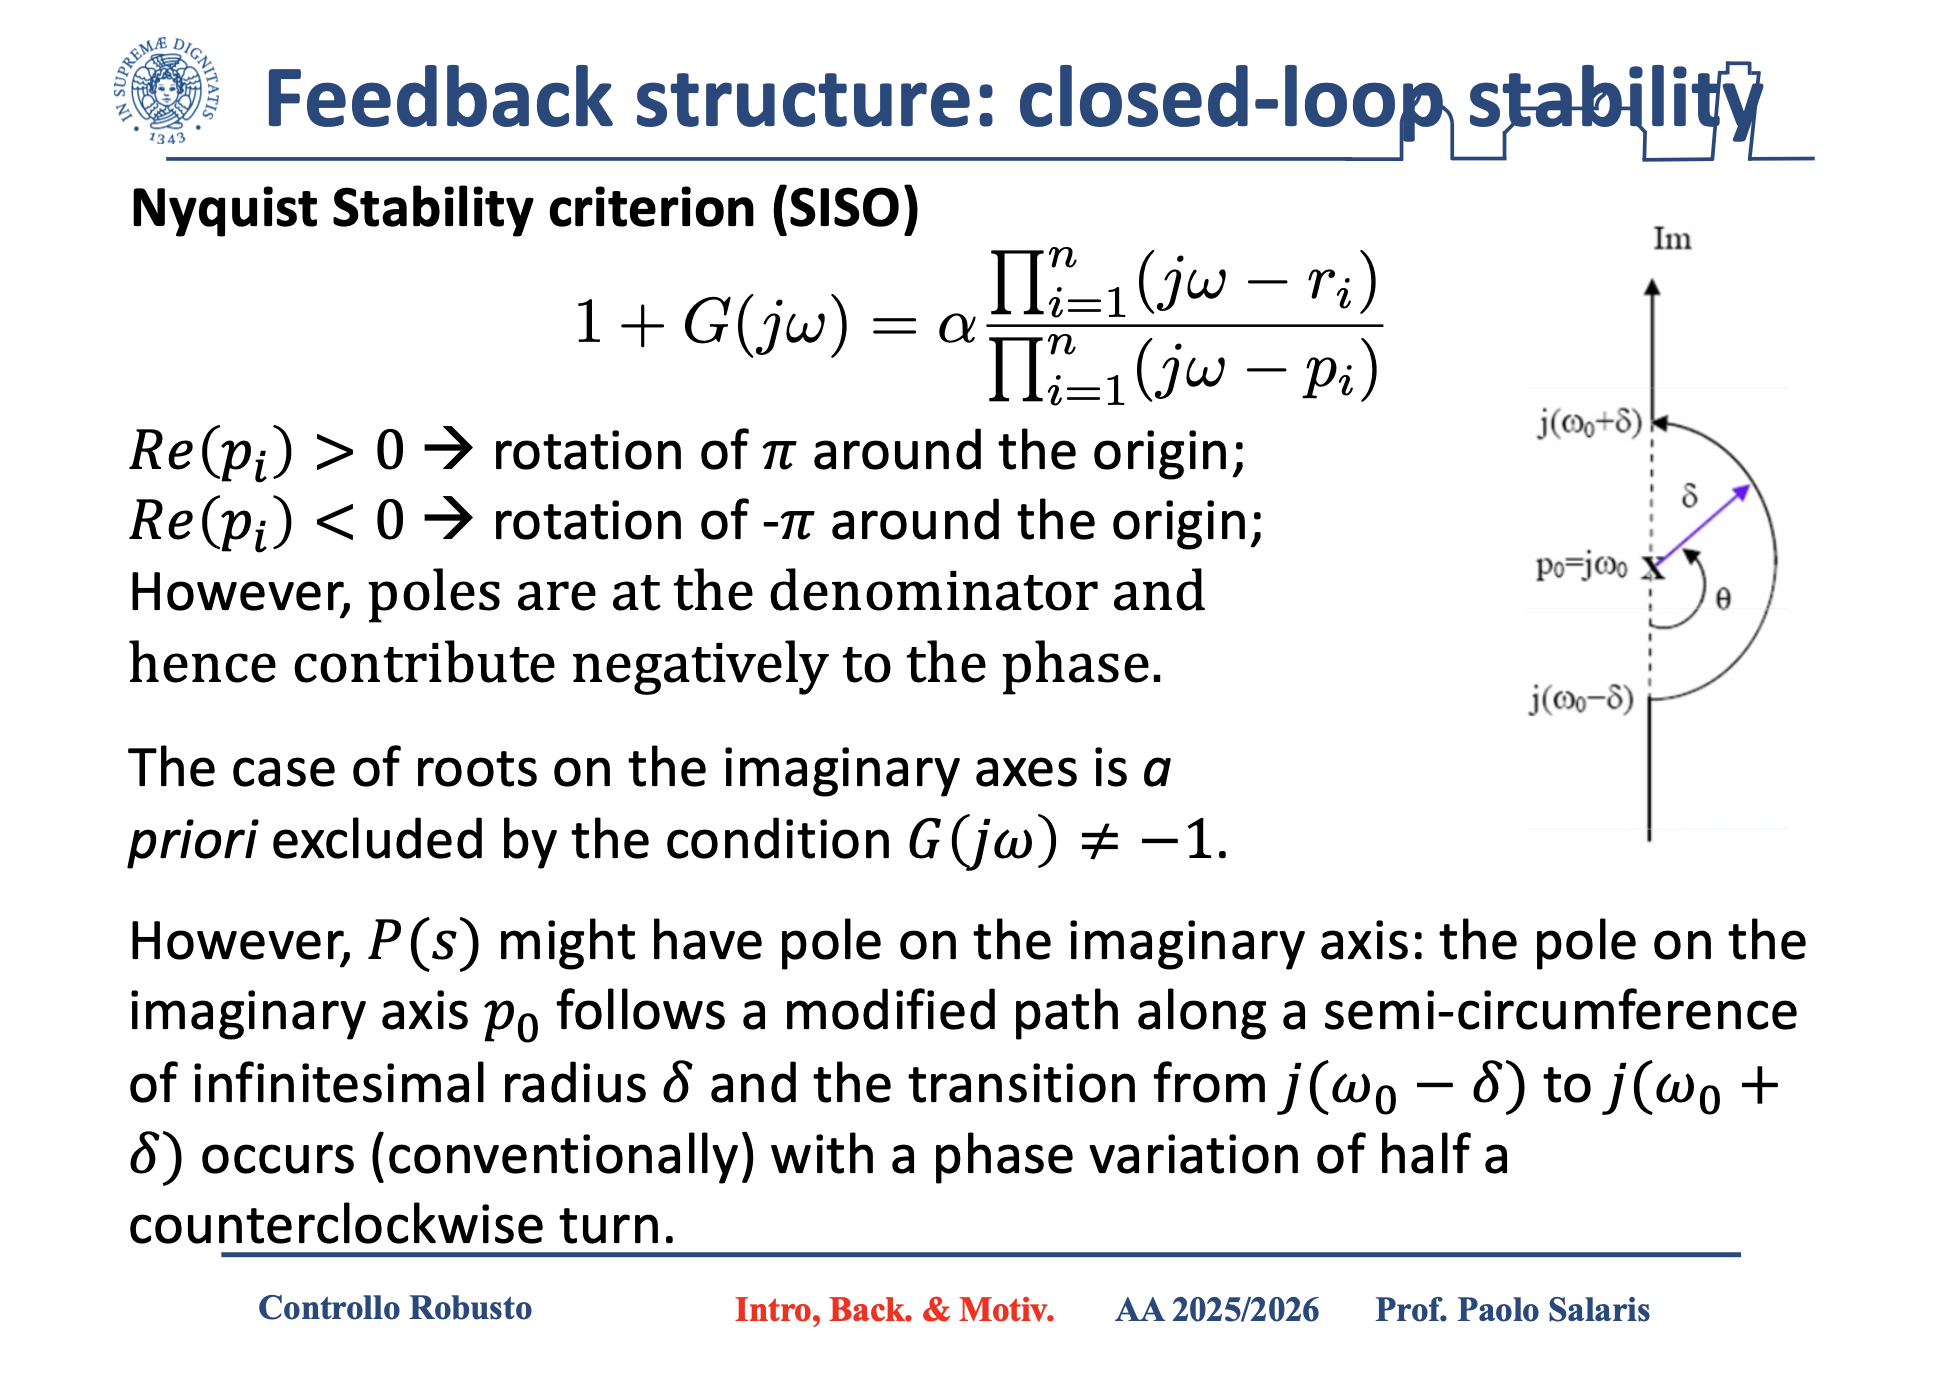
\includegraphics[width=\linewidth]{mancanti/Screenshot 2026-03-18 alle 15.25.41.png}
        \caption{Contributo in fase di poli e radici nel criterio di stabilità di Nyquist e definizione del percorso modificato per le singolarità sull'asse immaginario.}
    \end{subfigure}
    \hfill
    \begin{subfigure}{0.48\textwidth}
        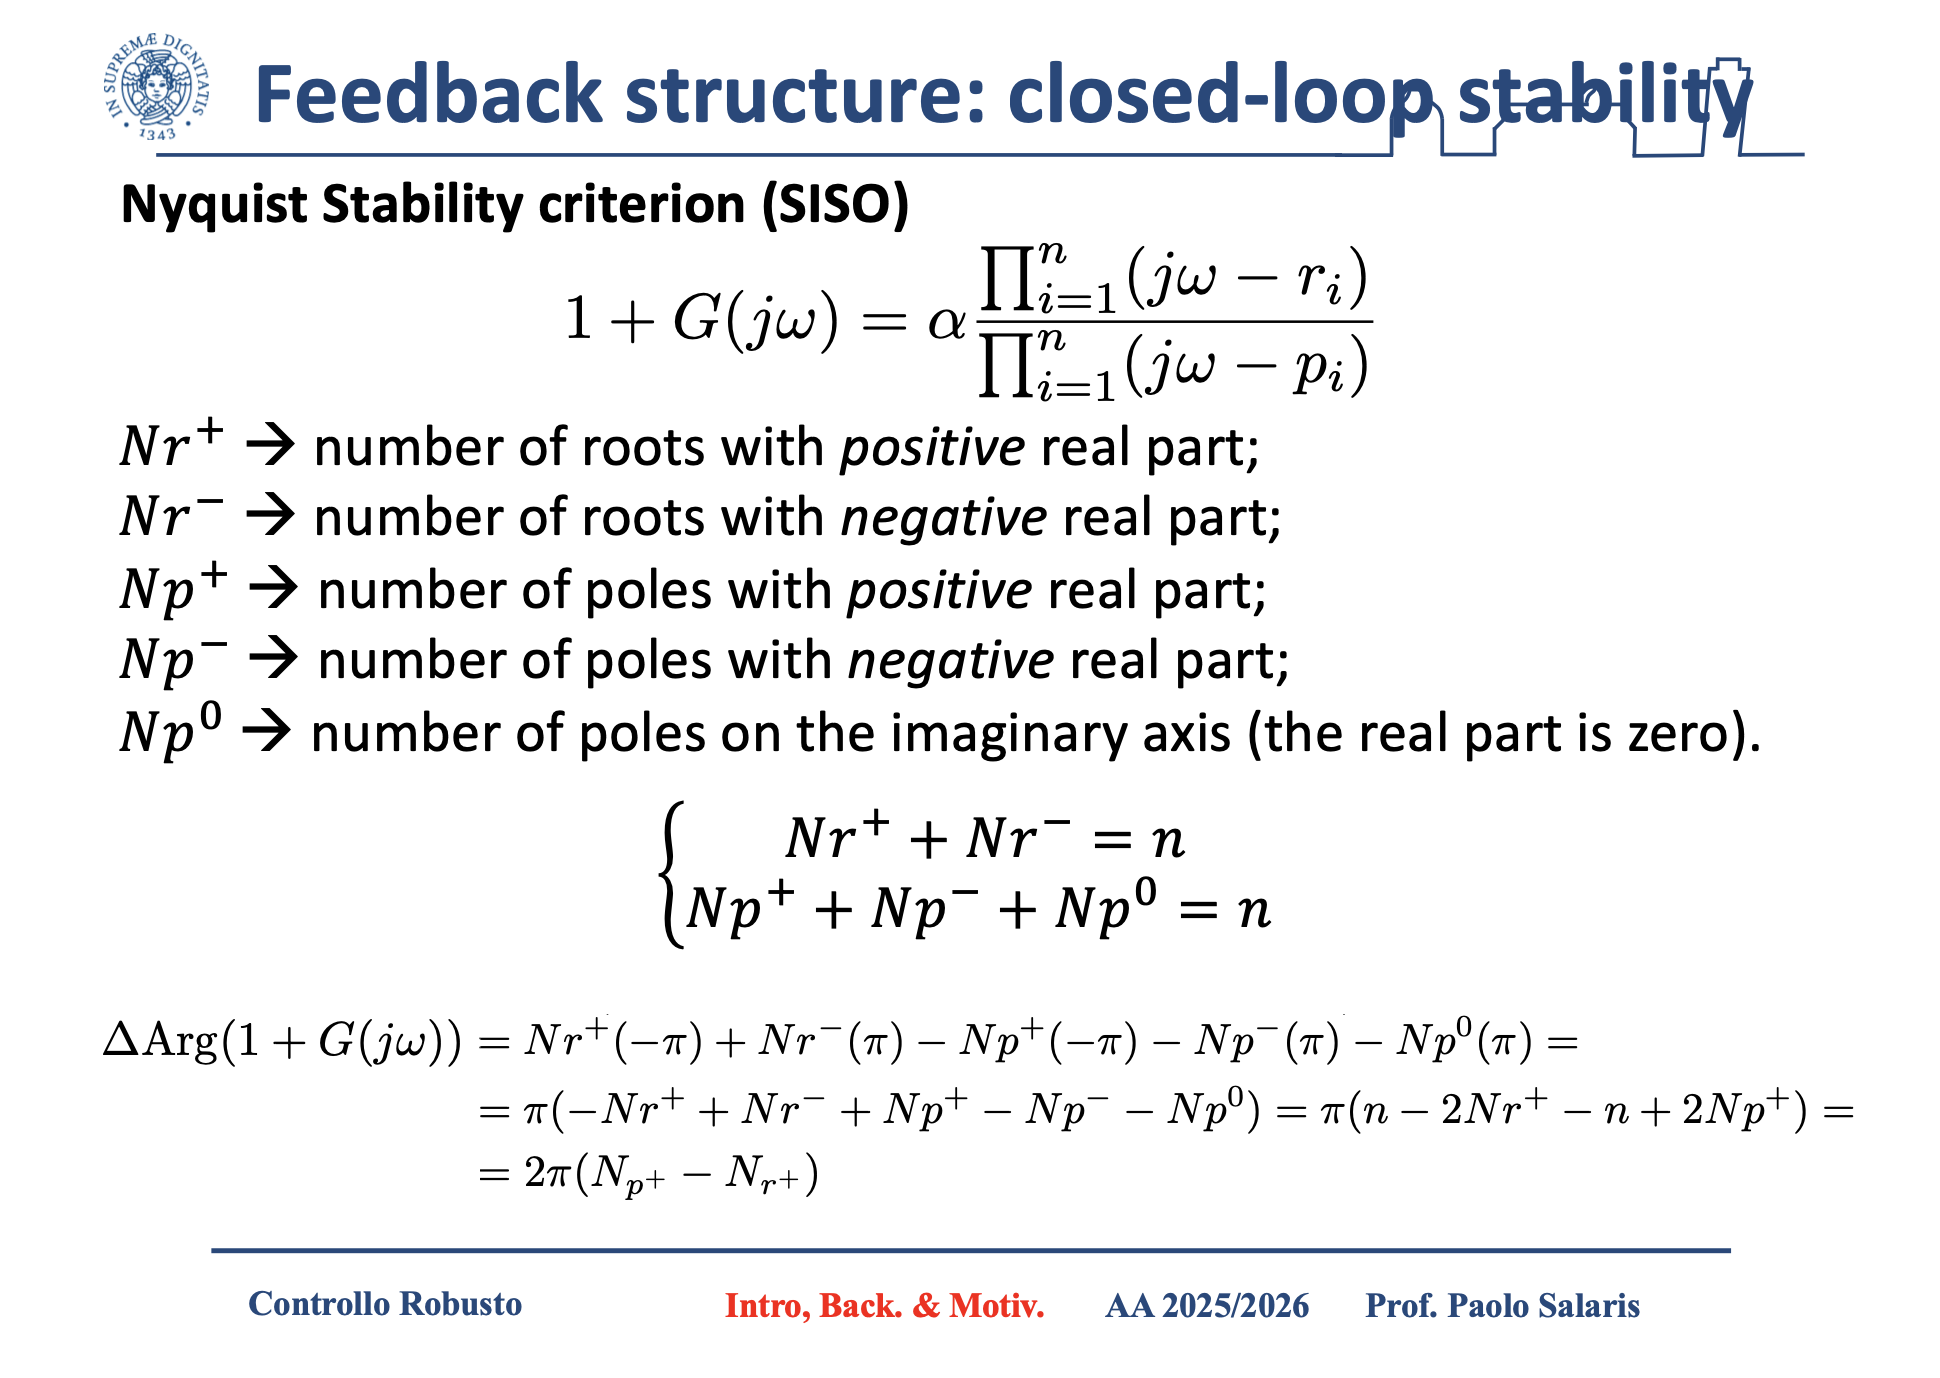
\includegraphics[width=\linewidth]{mancanti/Screenshot 2026-03-18 alle 15.26.06.png}
        \caption{Derivazione analitica della variazione totale dell'argomento $\Delta\text{Arg}(1 + G(j\omega))$ in funzione del numero di poli e radici a parte reale positiva e negativa.}
    \end{subfigure}
    \caption{Analisi della stabilità a ciclo chiuso mediante il criterio di Nyquist: valutazione dei contributi di fase locali (sinistra) e calcolo della variazione totale dell'argomento (destra).}
\end{figure}

Consideriamo una struttura standard a retroazione unitaria negativa, con funzione di trasferimento di anello aperto $G(s)$. La funzione di trasferimento in anello chiuso è
$$
T(s) = \frac{G(s)}{1+G(s)}.
$$

La stabilità asintotica del sistema chiuso dipende dalle radici dell’equazione caratteristica
$$
1 + G(s) = 0.
\label{eq:char_eq}
$$

Questa equazione è il vero oggetto del criterio di Nyquist. Infatti il criterio non lavora direttamente sui poli di $T(s)$, ma sulla variazione di argomento della funzione $1+G(s)$ lungo un opportuno contorno nel piano complesso della variabile $s$.

Supponiamo che
$$
1+G(j\omega) = \alpha \frac{\prod_{i=1}^{n}(j\omega-r_i)}{\prod_{i=1}^{n}(j\omega-p_i)},
$$
dove $r_i$ sono gli zeri di $1+G(s)$, cioè i poli dell’anello chiuso, e $p_i$ sono i poli di $G(s)$, cioè i poli dell’anello aperto. Ogni fattore del tipo $(j\omega-r_i)$ o $(j\omega-p_i)$ contribuisce alla variazione complessiva di fase quando $\omega$ percorre l’asse immaginario.

\subsection{Principio dell’argomento e interpretazione geometrica}
\label{sec:arg}
\begin{figure}[H]
    \centering
    \begin{subfigure}{0.48\textwidth}
        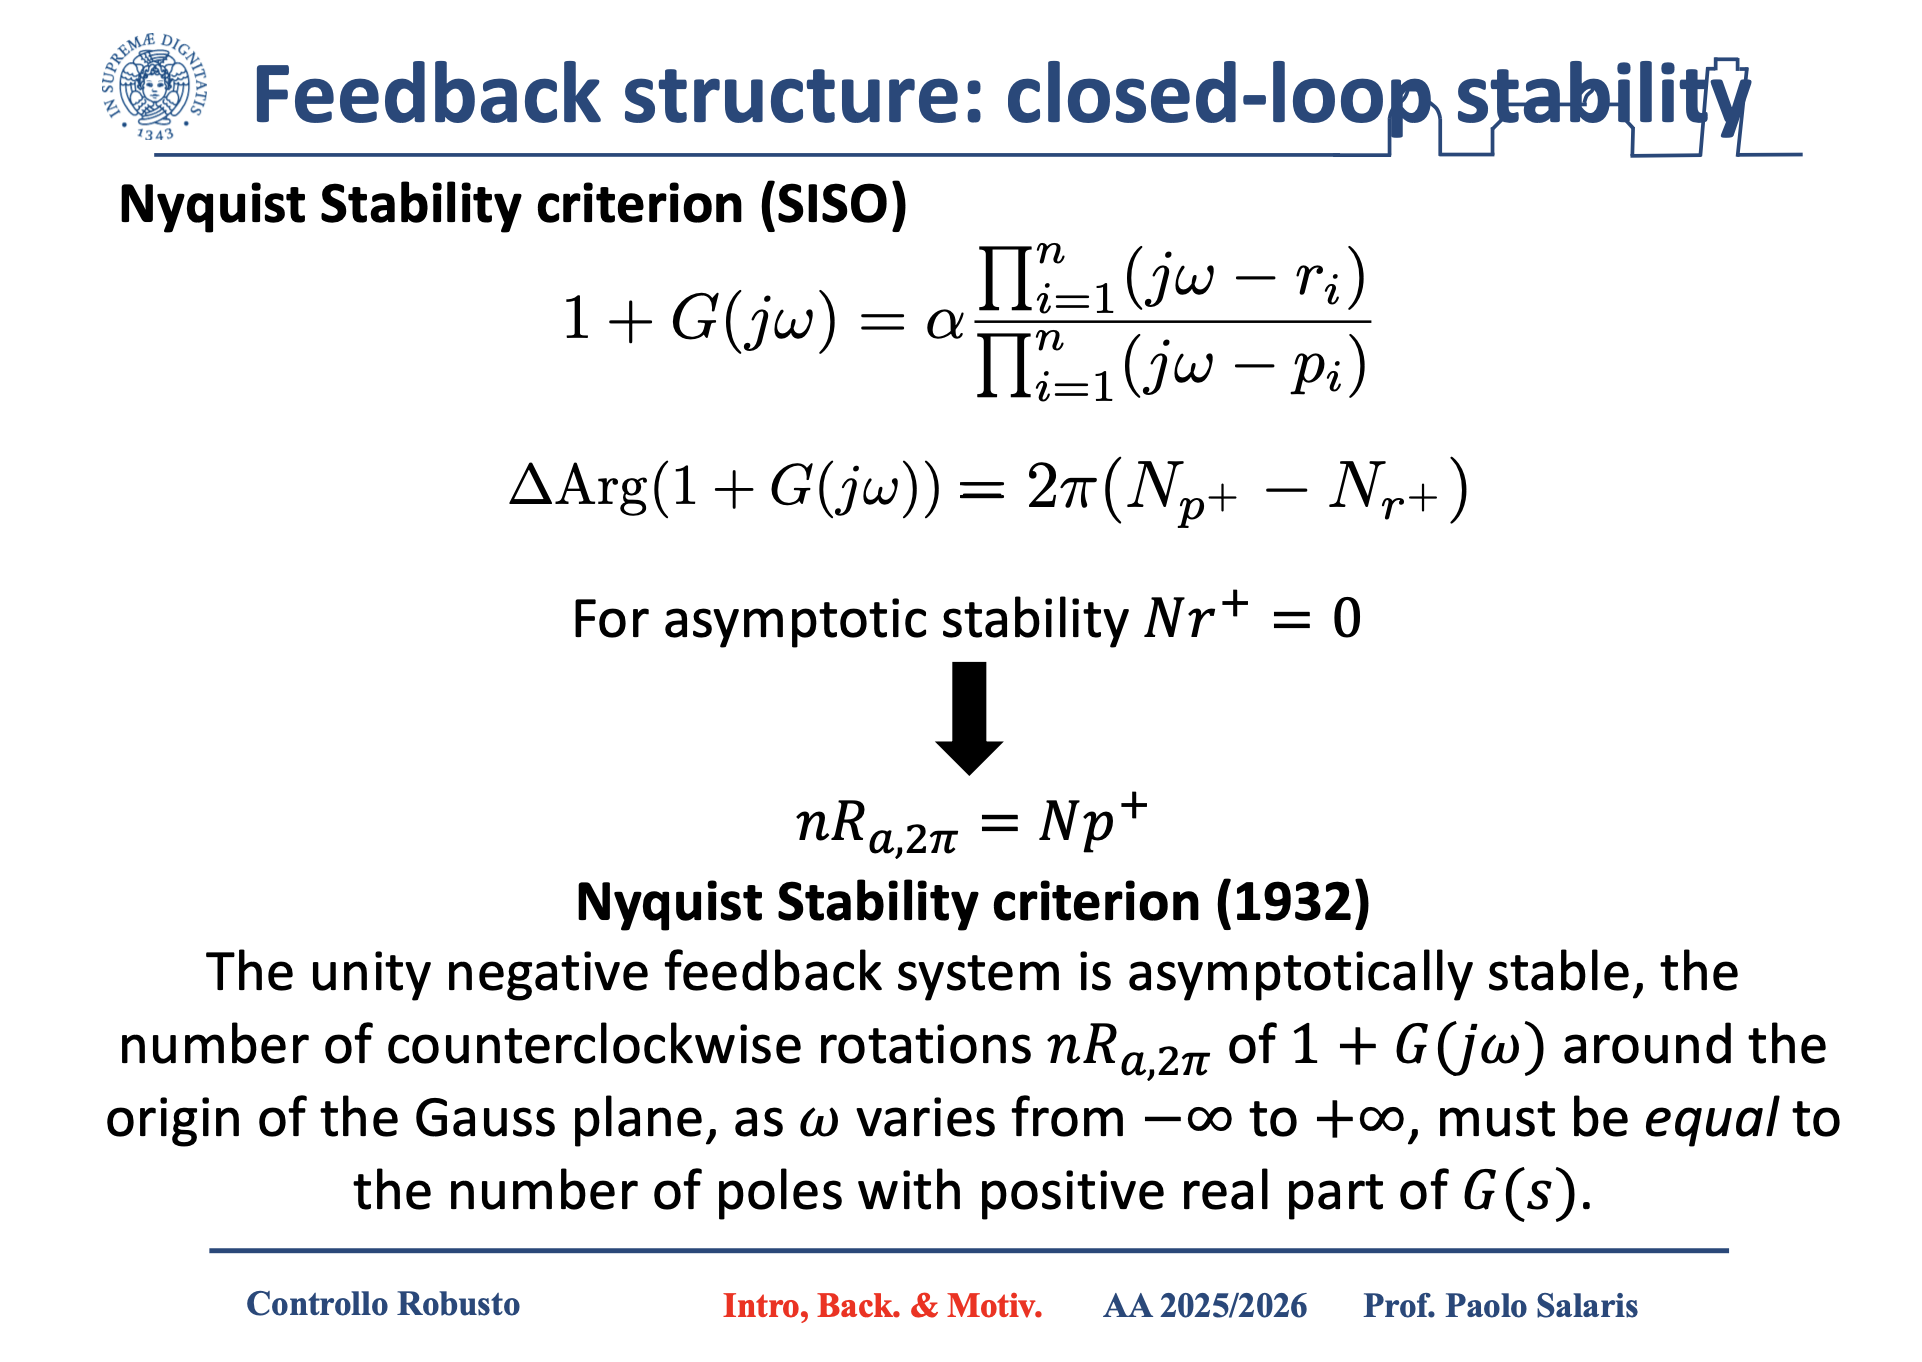
\includegraphics[width=\linewidth]{mancanti/Screenshot 2026-03-18 alle 15.26.20.png}
        \caption{Enunciazione formale del Criterio di Stabilità di Nyquist: condizione di stabilità asintotica espressa come uguaglianza tra il numero di rotazioni antiorarie $nR_{a,2\pi}$ e il numero di poli a ciclo aperto a parte reale positiva $Np^+$.}
    \end{subfigure}
    \hfill
    \begin{subfigure}{0.48\textwidth}
        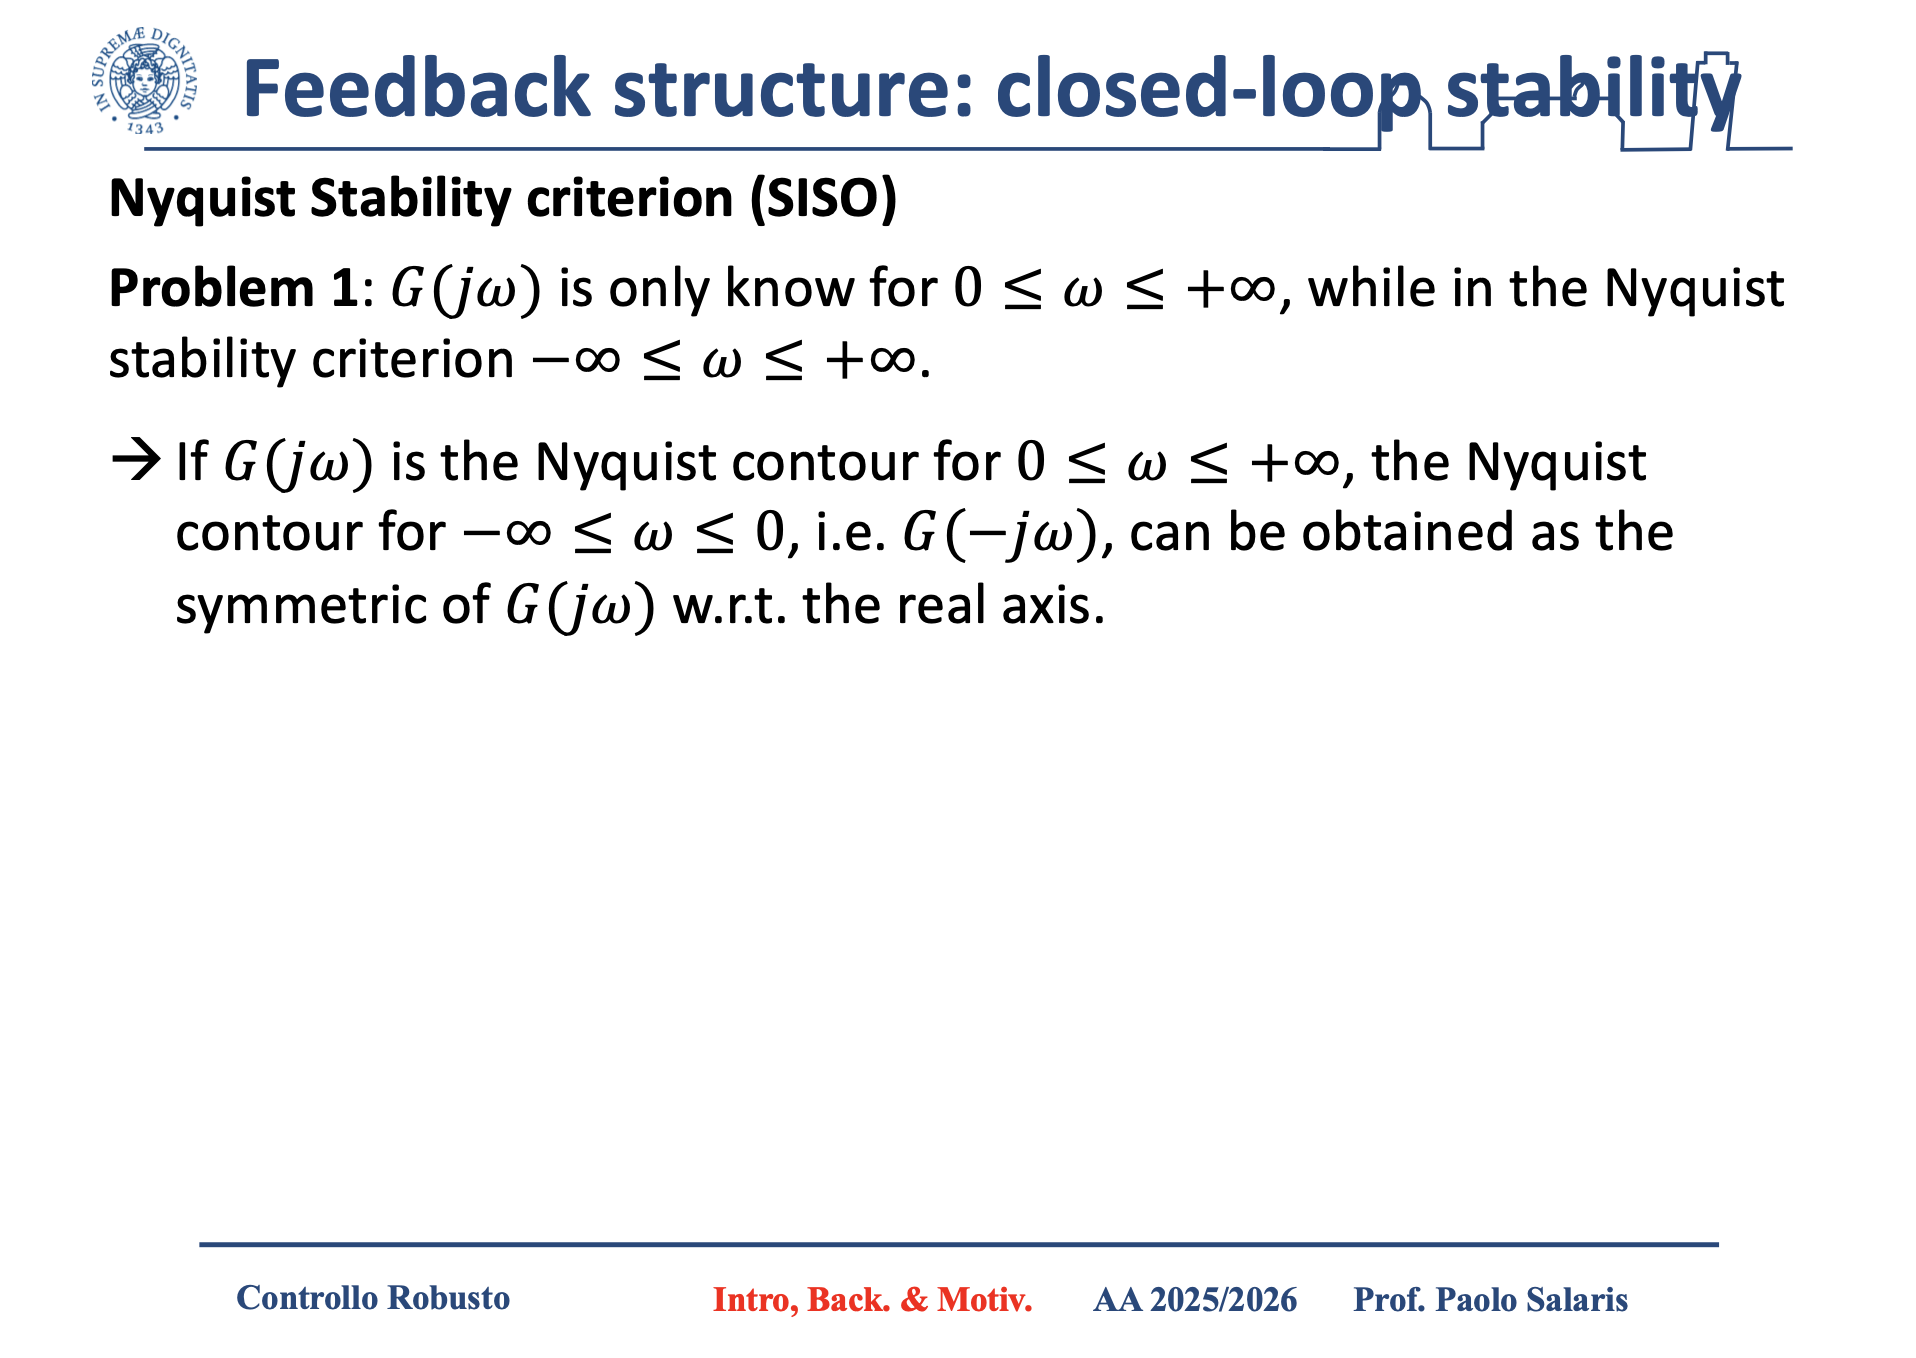
\includegraphics[width=\linewidth]{mancanti/Screenshot 2026-03-18 alle 15.26.35.png}
        \caption{Proprietà di simmetria del diagramma di Nyquist: costruzione del percorso per frequenze negative ($-\infty \leq \omega \leq 0$) tramite ribaltamento speculare rispetto all'asse reale.}
    \end{subfigure}
    \caption{Definizione del Criterio di Stabilità di Nyquist per sistemi a ciclo chiuso (sinistra) e completamento del tracciato polar per frequenze negative sfruttando la simmetria complessa coniugata (destra).}
\end{figure}

Il cuore matematico del criterio di Nyquist è il \emph{principio dell’argomento}. In forma intuitiva, esso afferma che la variazione totale di fase di una funzione razionale lungo un contorno chiuso è proporzionale alla differenza fra il numero di zeri e il numero di poli interni al contorno, contati con molteplicità.

Applicato alla funzione $1+G(s)$ e al semipiano destro, il principio dell’argomento consente di contare quanti poli dell’anello chiuso hanno parte reale positiva senza risolvere esplicitamente l’equazione caratteristica. Se indichiamo con:
\begin{itemize}
    \item $N_r^+$ il numero di radici di $1+G(s)$ nel semipiano destro,
    \item $N_r^-$ il numero di radici nel semipiano sinistro,
    \item $N_p^+$ il numero di poli di $G(s)$ nel semipiano destro,
    \item $N_p^-$ il numero di poli nel semipiano sinistro,
    \item $N_p^0$ il numero di poli di $G(s)$ sull’asse immaginario,
\end{itemize}
allora la variazione di argomento lungo il contorno di Nyquist può essere ricondotta alla relazione mostrata nelle slide:
$$
\Delta \operatorname{Arg}(1+G(j\omega)) = 2\pi\,(N_r^+ - N_p^+),
\label{eq:arg_relation_standard}
$$
con una convenzione sui segni che dipende dal verso di percorrenza del contorno e da come viene contato il numero di avvolgimenti. Nelle slide il conteggio è espresso come numero di rotazioni antiorarie di $1+G(j\omega)$ attorno all’origine, oppure in modo equivalente come numero di avvolgimenti di $G(j\omega)$ attorno al punto $-1$.

\begin{keybox}
La stabilità asintotica in anello chiuso richiede $N_r^+=0$. Il criterio di Nyquist trasforma quindi un problema algebrico sui poli del chiuso in un problema geometrico di avvolgimenti nel piano complesso.
\end{keybox}

Per capire perché il criterio funziona, si può leggere ogni termine $(j\omega-a)$ come un vettore che va dal punto $a$ del piano complesso al punto variabile $j\omega$ sull’asse immaginario. Quando $\omega$ va da $-\infty$ a $+\infty$, il vettore ruota di un certo angolo netto:
\begin{itemize}
    \item se $a$ si trova nel semipiano destro, il contributo è di $-\pi$ per uno zero e cambia di segno per un polo perché il termine appare al denominatore;
    \item se $a$ si trova nel semipiano sinistro, il contributo è di $+\pi$ per uno zero, ancora con segno opposto nel caso di un polo.
\end{itemize}

La somma di tutti questi contributi porta esattamente al conteggio in \eqref{eq:arg_relation_standard}.

\subsection{Enunciato del criterio di Nyquist nel caso SISO}

Nel caso di retroazione unitaria negativa, il sistema in anello chiuso è asintoticamente stabile se e solo se il numero di rotazioni antiorarie del luogo di $1+G(j\omega)$ attorno all’origine, al variare di $\omega$ da $-\infty$ a $+\infty$, coincide con il numero di poli instabili di $G(s)$.

Equivalentemente, poiché traslare di $1$ il luogo di $G(j\omega)$ corrisponde a passare da $G(j\omega)$ a $1+G(j\omega)$, il criterio si può formulare nella forma più nota:
\begin{quote}
Il luogo di Nyquist di $G(j\omega)$ deve circondare il punto critico $-1$ un numero di volte pari al numero di poli di $G(s)$ nel semipiano destro, con il verso imposto dalla convenzione adottata.
\end{quote}

Nelle slide il conteggio viene espresso mediante il numero di rotazioni $n_{R_{+,2\pi}}$; il contenuto fisico è sempre lo stesso: la curva in frequenza deve compensare esattamente l’instabilità presente in anello aperto per produrre un sistema chiuso stabile.

\subsubsection{Perché il punto critico è proprio \texorpdfstring{$-1$}{-1}}

Il punto $-1$ non è una scelta arbitraria. Dall’equazione caratteristica \eqref{eq:char_eq} si vede subito che i poli dell’anello chiuso si hanno esattamente quando $G(s)=-1$. In frequenza, il punto $-1$ rappresenta quindi il valore critico che rende singolare il denominatore $1+G(s)$. Se il luogo di Nyquist passa attraverso o avvolge quel punto in modo scorretto, il sistema chiuso può perdere stabilità.

\subsubsection{Problema operativo 1: conosciamo solo \texorpdfstring{$G(j\omega)$ per $\omega\ge 0$}{G(jw) per w>=0}}

Nella pratica sperimentale o numerica, la risposta in frequenza viene spesso tracciata solo per frequenze non negative. Tuttavia il criterio di Nyquist richiede, in linea teorica, il percorso per $\omega \in (-\infty,+\infty)$. La soluzione sfrutta la simmetria dei sistemi a coefficienti reali:
$$
G(-j\omega) = \overline{G(j\omega)}.
$$

Di conseguenza, il tratto per frequenze negative si ottiene come simmetrico rispetto all’asse reale del tratto per frequenze positive. Questo fatto giustifica la classica rappresentazione del luogo di Nyquist come curva superiore per $\omega>0$ e curva inferiore come immagine speculare.

Questa osservazione sembra banale, ma è decisiva dal punto di vista pratico: permette di costruire il contorno completo a partire da metà delle informazioni disponibili.

\subsubsection{Problema operativo 2: poli sull’asse immaginario}
\label{sec:imagaxis}

Il criterio classico richiede che il contorno non attraversi singolarità della funzione. Se $G(s)$ ha poli esattamente sull’asse immaginario, il cammino standard lungo $s=j\omega$ non è più ammissibile. In quel caso si deforma il contorno aggirando il polo con una semicirconferenza di raggio infinitesimo nel piano di destra.

La slide corrispondente mostra due idee importanti:
\begin{enumerate}
    \item localmente, in prossimità del polo sull’asse immaginario, il percorso viene deviato con una piccola semicirconferenza;
    \item nel piano di Nyquist, questa deviazione si traduce in una \emph{closure at infinity}, cioè in un arco a raggio infinito percorso in senso orario.
\end{enumerate}

\begin{figure}[H]
    \centering
    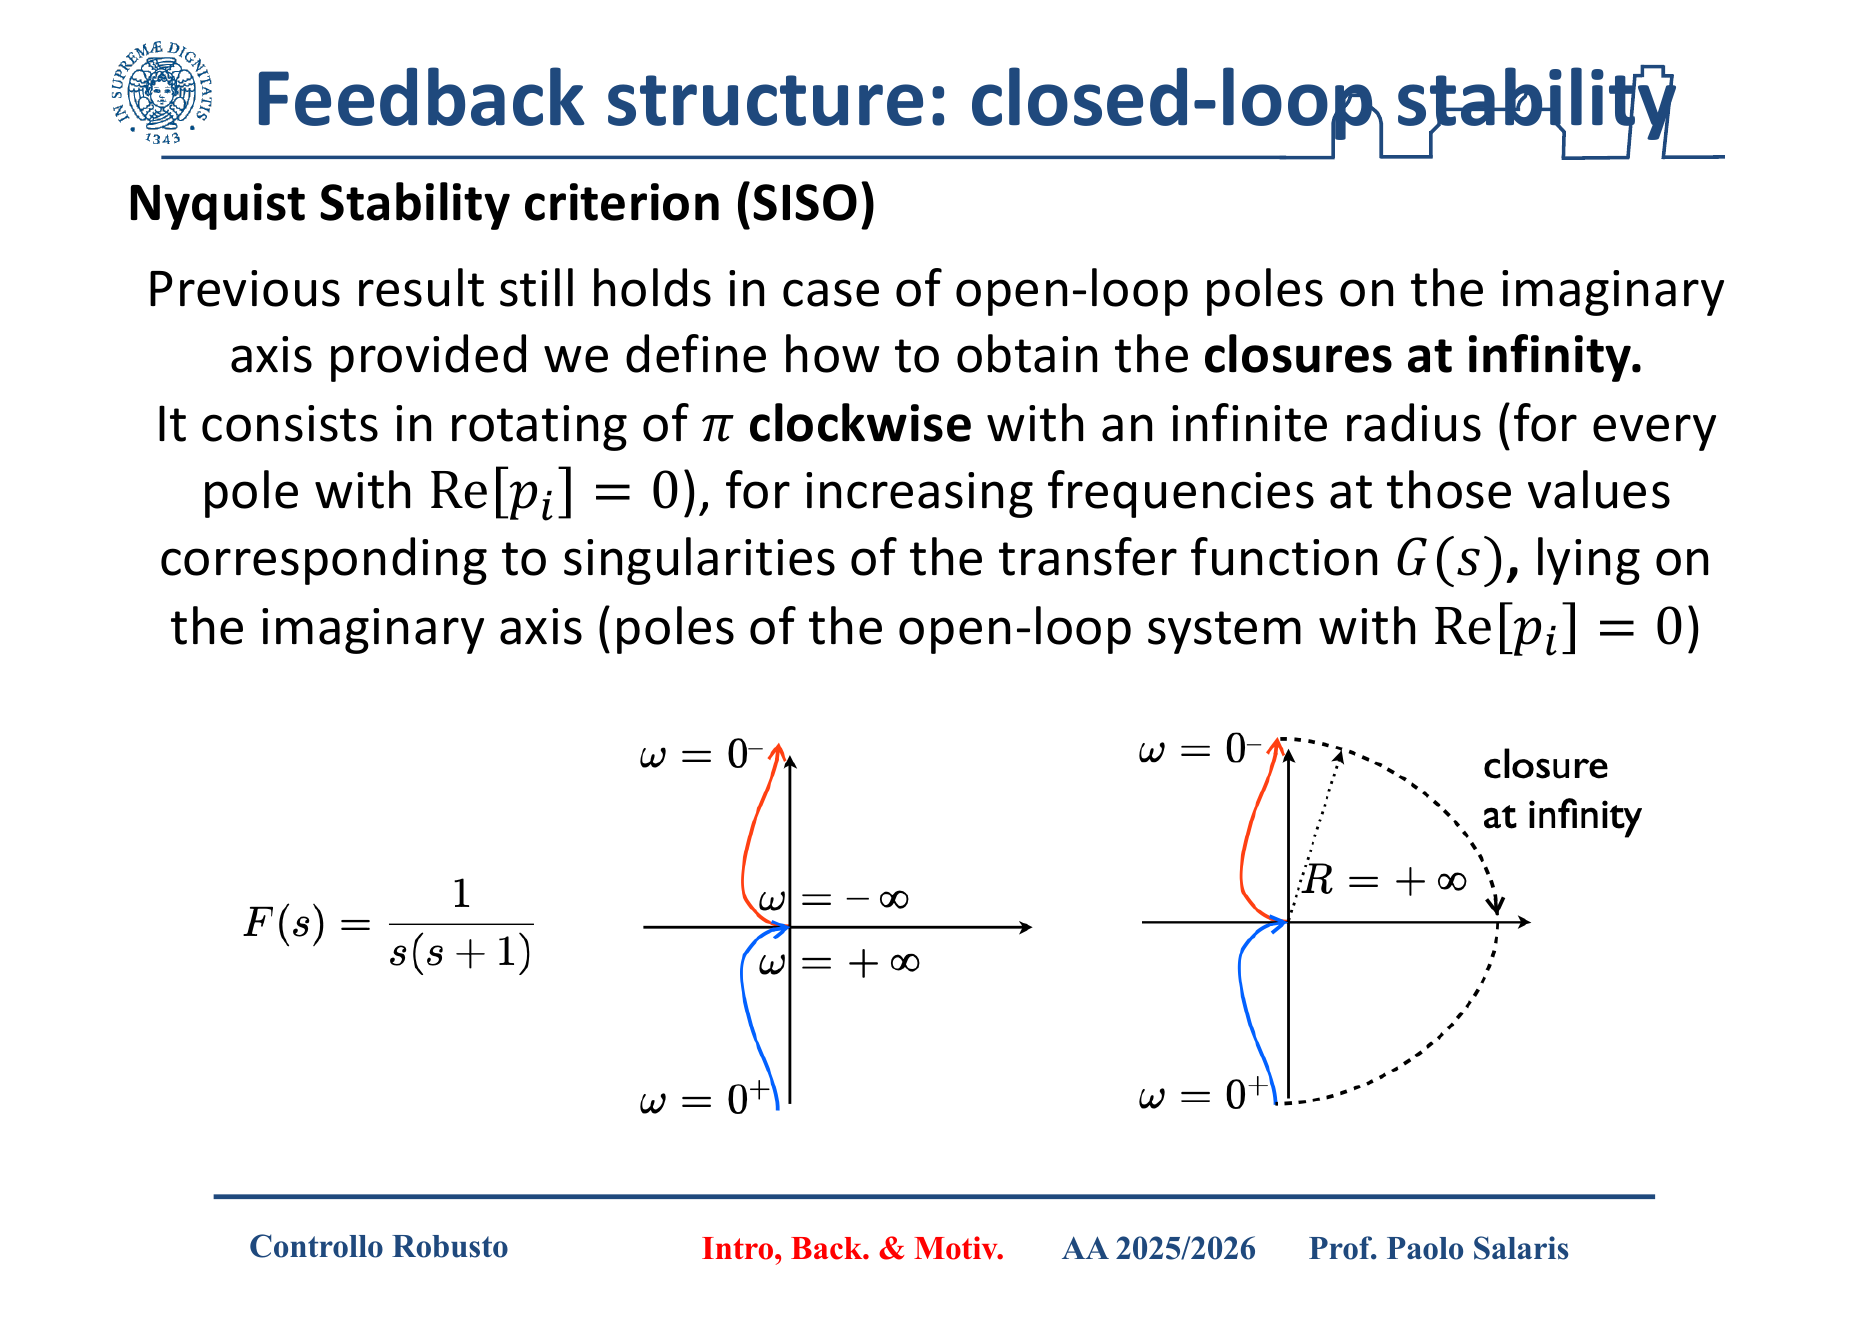
\includegraphics[width=0.82\textwidth]{images/nyquist_imag_axis.png}
    \caption{Slide originale che illustra la gestione di un polo in anello aperto sull’asse immaginario e la corrispondente chiusura all’infinito.}
    \label{fig:imag_axis}
\end{figure}

Dal punto di vista concettuale, questa costruzione evita di attribuire impropriamente al sistema una variazione di fase non definita nel punto singolare. Il principio dell’argomento continua a valere, ma il contorno deve essere scelto in modo da non attraversare poli.

Un caso tipico è
$$
F(s)=\frac{1}{s(s+1)},
$$
che ha un polo nell’origine. Quando $s$ percorre una piccola semicirconferenza nel piano di destra attorno a $s=0$, l’immagine tramite $F(s)$ produce un grande arco nel piano complesso. Quel grande arco chiude il luogo di Nyquist e va incluso nel conteggio degli avvolgimenti.

\subsubsection{Dalla forma \texorpdfstring{$1+G(j\omega)$}{1+G(jw)} alla forma di Evans}

Un’altra difficoltà pratica è che spesso si conosce o si traccia il luogo di $G(j\omega)$, non quello di $1+G(j\omega)$. La traslazione geometrica risolve il problema. Infatti:
$$
1 + K G(j\omega)
$$
ruota attorno all’origine tante volte quante $K G(j\omega)$ ruota attorno al punto $-1$. Se $K>0$ è reale, si può anche dire che $G(j\omega)$ ruota attorno al punto $-1/K$.

Questa forma è estremamente utile in progettazione, perché consente di ragionare direttamente su come il guadagno $K$ sposta il punto critico lungo l’asse reale. In sostanza:
\begin{itemize}
    \item fissato il luogo di $G(j\omega)$, cambiare $K$ equivale a cambiare il punto critico da osservare;
    \item fissato il punto $-1$, cambiare $K$ equivale a riscalare radialmente il luogo di Nyquist.
\end{itemize}

Questa è esattamente la stessa filosofia del luogo delle radici: si vuole capire per quali valori del guadagno la chiusura in retroazione rimane stabile.

\subsection{Esempi SISO: lettura geometrica dei luoghi di Nyquist}
\label{sec:examples_siso}

Le slide riportano numerosi esempi. Qui li riorganizziamo in modo ragionato, evidenziando cosa bisogna osservare in ogni figura.

\subsubsection{Famiglia di esempi con poli stabili e zero a destra}

La prima slide di esempi confronta due funzioni:
$$
G_1(s)=\frac{10}{(s+1)^2(s+10)},
\qquad
G_2(s)=\frac{-10(s-1)}{(s+1)^2(s+10)}.
$$

\begin{figure}[H]
    \centering
    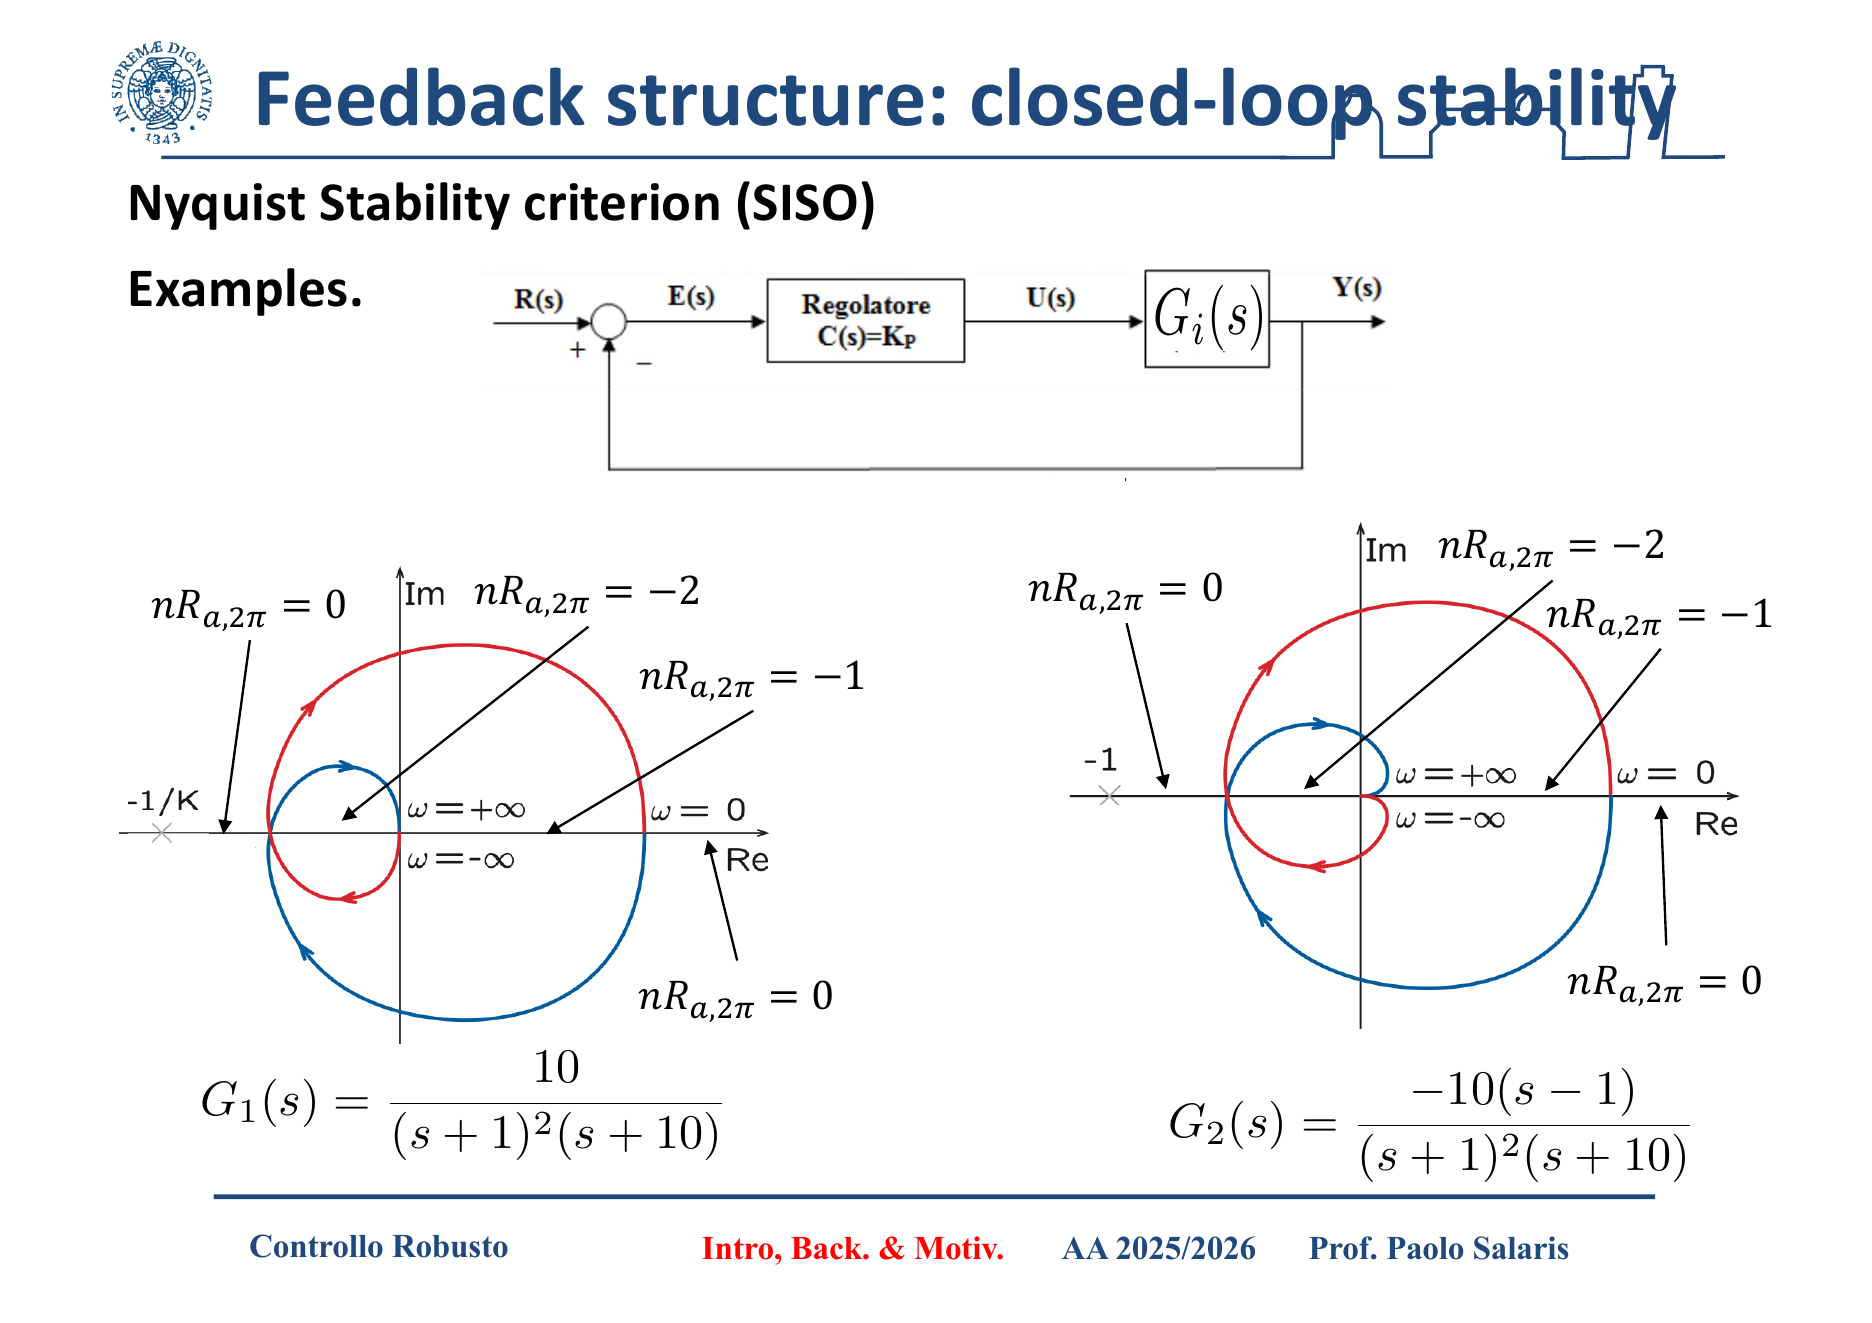
\includegraphics[width=0.92\textwidth]{images/nyquist_examples_pair.png}
    \caption{Confronto fra due luoghi di Nyquist: il secondo caso introduce uno zero nel semipiano destro e modifica in modo significativo la topologia del luogo.}
    \label{fig:pair_examples}
\end{figure}

Il primo caso ha tutti i poli nel semipiano sinistro e nessuno zero a destra. Il luogo tende a curve relativamente regolari; il criterio consiste nel verificare se, per il valore di guadagno scelto, il punto $-1/K$ viene circondato o meno. Nel secondo caso compare il fattore $(s-1)$, cioè uno zero nel semipiano destro. Gli zeri non entrano direttamente nel conteggio di Nyquist come i poli dell’anello aperto, ma alterano profondamente la forma del luogo, rendendo possibile un maggior numero di avvolgimenti del punto critico.

Questo esempio è istruttivo perché mostra che non basta conoscere il numero di poli instabili di $G(s)$: la geometria complessiva di $G(j\omega)$ dipende da tutta la struttura della funzione di trasferimento.

\subsubsection{Esempio \texorpdfstring{$\boldsymbol{2/(s-1)}$}{2/(s-1)}}

Consideriamo
$$
G(s)=\frac{2}{s-1}.
$$

Il polo in $s=1$ è instabile. Quindi l’anello aperto ha $N_p^+=1$. Per ottenere stabilità in anello chiuso, il luogo di Nyquist deve compensare esattamente questa instabilità con un avvolgimento appropriato del punto critico.

\begin{figure}[H]
    \centering
    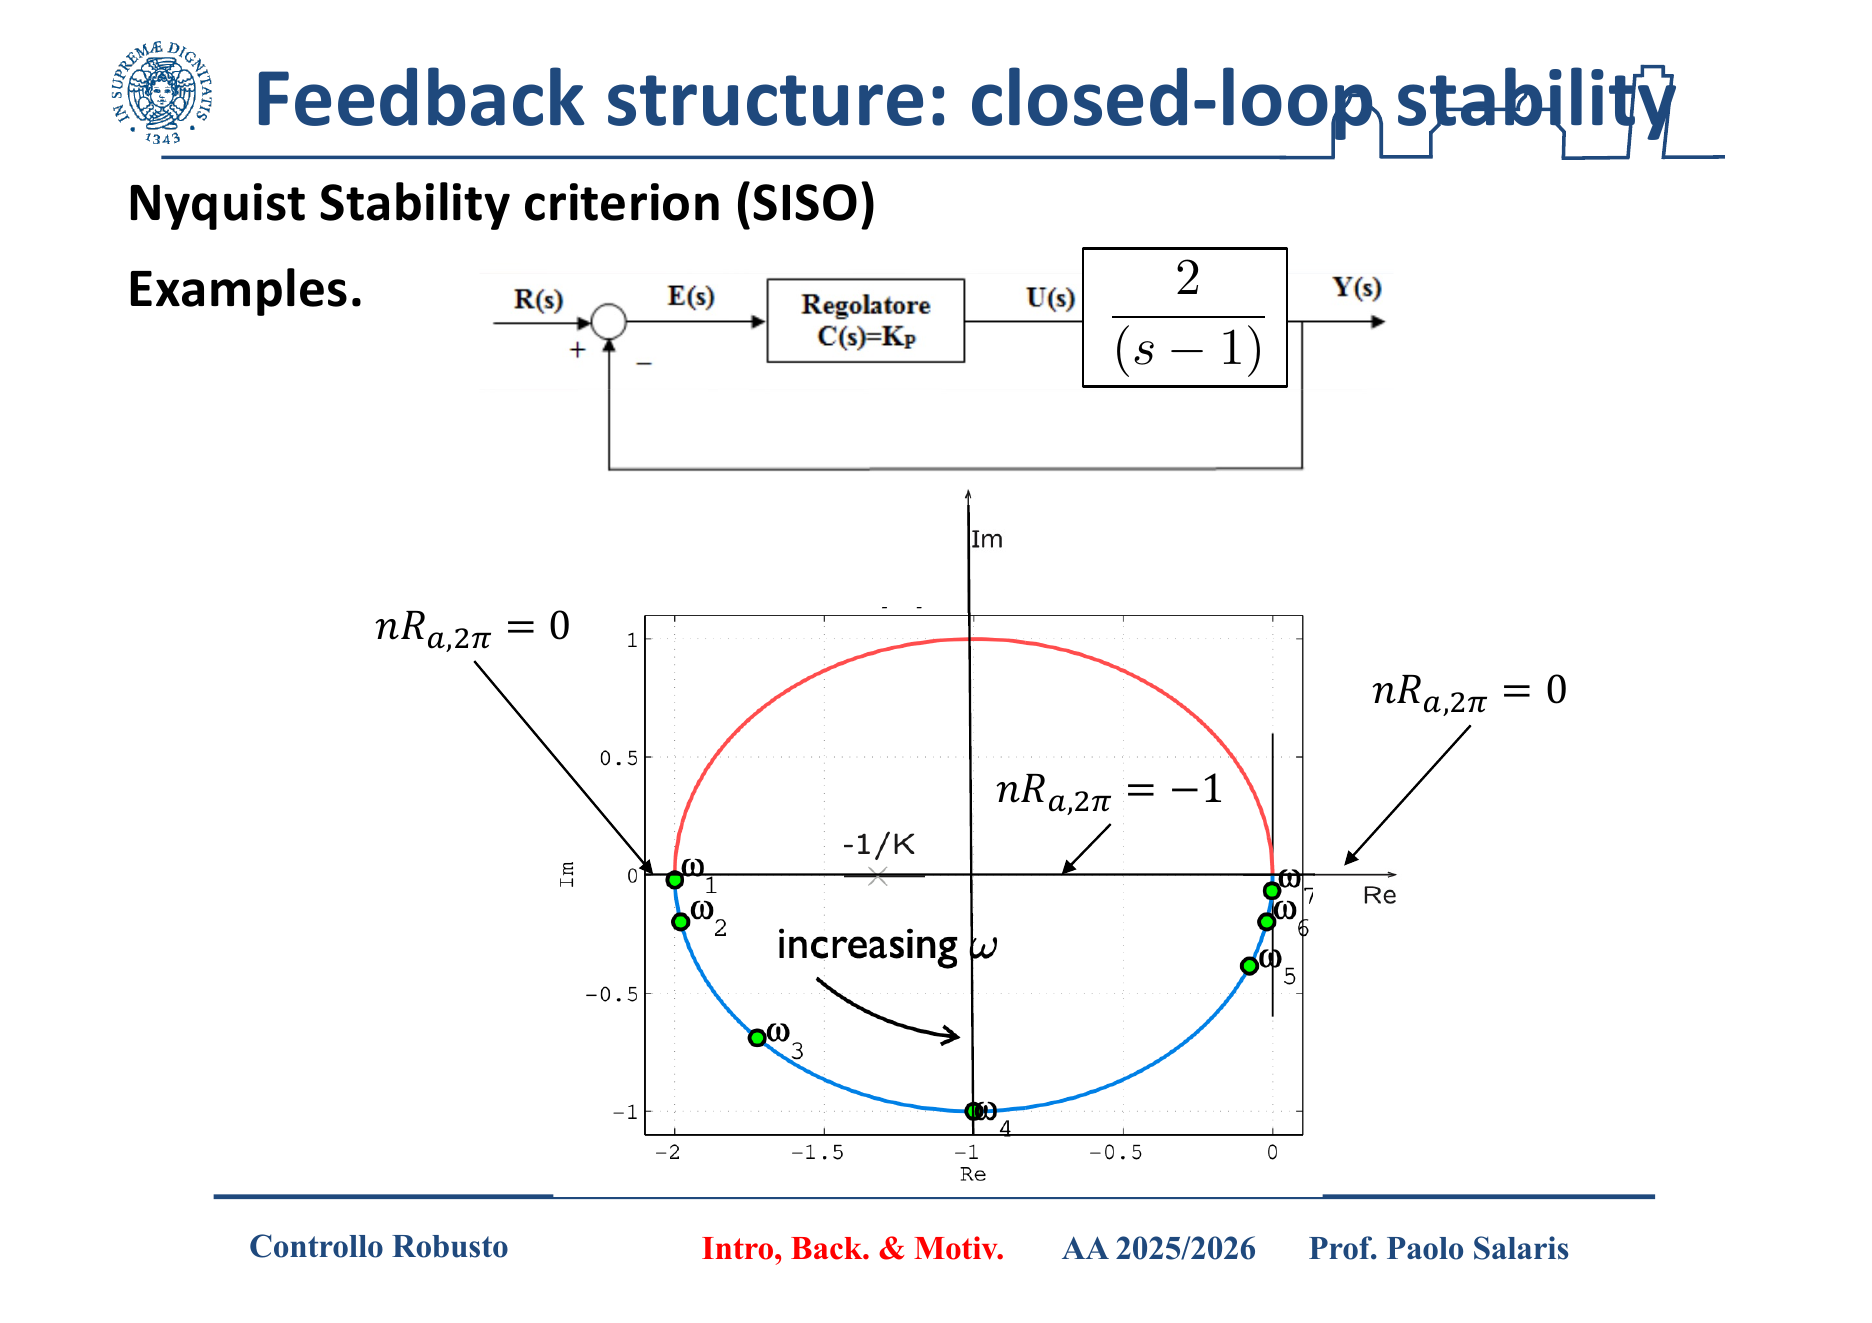
\includegraphics[width=0.66\textwidth]{images/example_2_over_sminus1.png}
    \caption{Luogo di Nyquist per $G(s)=2/(s-1)$. La presenza di un polo a destra impone un conteggio degli avvolgimenti coerente con $N_p^+=1$.}
    \label{fig:2_over_sminus1}
\end{figure}

Geometricamente il luogo è un cerchio nel piano complesso. Il punto chiave è che non conta soltanto se il luogo passa a sinistra o a destra del punto critico: conta il numero netto di avvolgimenti, con orientazione.

\subsubsection{Esempio con integratore: \texorpdfstring{$\boldsymbol{100/(s(s+10)^2)}$}{100 over s times (s+10) squared}}

Consideriamo
$$
G(s)=\frac{100}{s(s+10)^2}.
$$

Qui compare un polo nell’origine. Questo significa che, come discusso in \S\ref{sec:imagaxis}, il contorno standard deve essere modificato e il luogo di Nyquist include una chiusura all’infinito. L’effetto visivo si vede chiaramente nella slide: oltre ai rami principali, compare un arco grande che rappresenta l’immagine della deviazione attorno al polo su asse immaginario.

\begin{figure}[H]
    \centering
    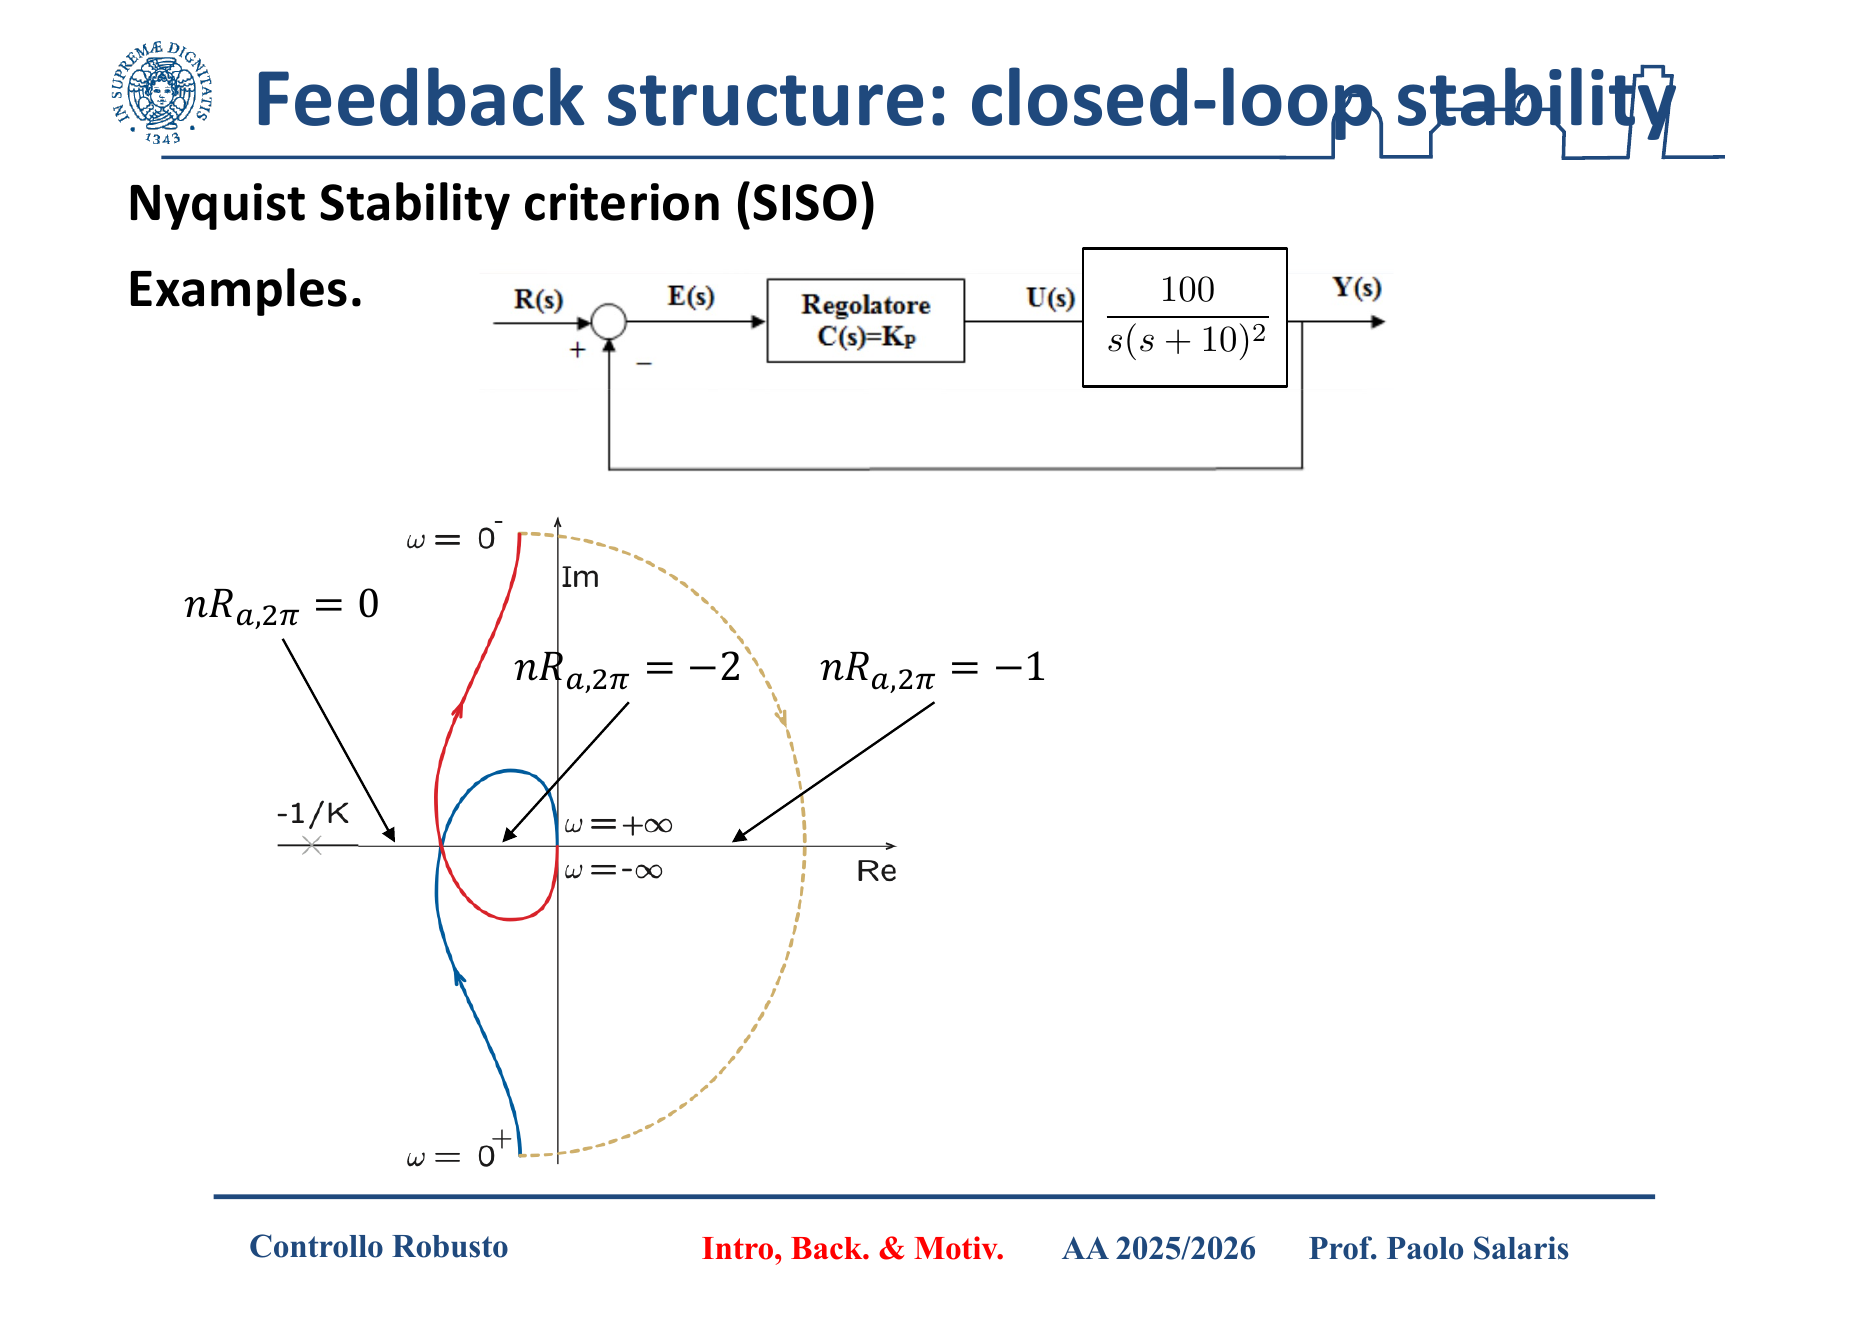
\includegraphics[width=0.68\textwidth]{images/example_100_over_s_splus10_sq.png}
    \caption{Esempio con polo nell’origine. La chiusura all’infinito contribuisce al conteggio degli avvolgimenti.}
    \label{fig:integrator_example}
\end{figure}

Questo caso è importante in automazione perché gli integratori sono molto comuni. Un errore tipico è dimenticare il contributo della deviazione attorno al polo nell’origine: il conteggio finale degli avvolgimenti risulterebbe sbagliato e la conclusione sulla stabilità sarebbe errata.

\subsubsection{Esempio con poli immaginari puri: \texorpdfstring{$\boldsymbol{1/((s+1)(s^2+1))}$}{1 over (s+1)(s squared+1)}}

La funzione
$$
G(s)=\frac{1}{(s+1)(s^2+1)}
$$
ha poli in $s=\pm j$ oltre al polo stabile in $-1$. I poli puramente immaginari richiedono nuovamente la deformazione del contorno. In termini geometrici, il luogo di Nyquist presenta rami che si dirigono all’infinito in corrispondenza delle frequenze singolari $\omega=\pm 1$.

\begin{figure}[H]
    \centering
    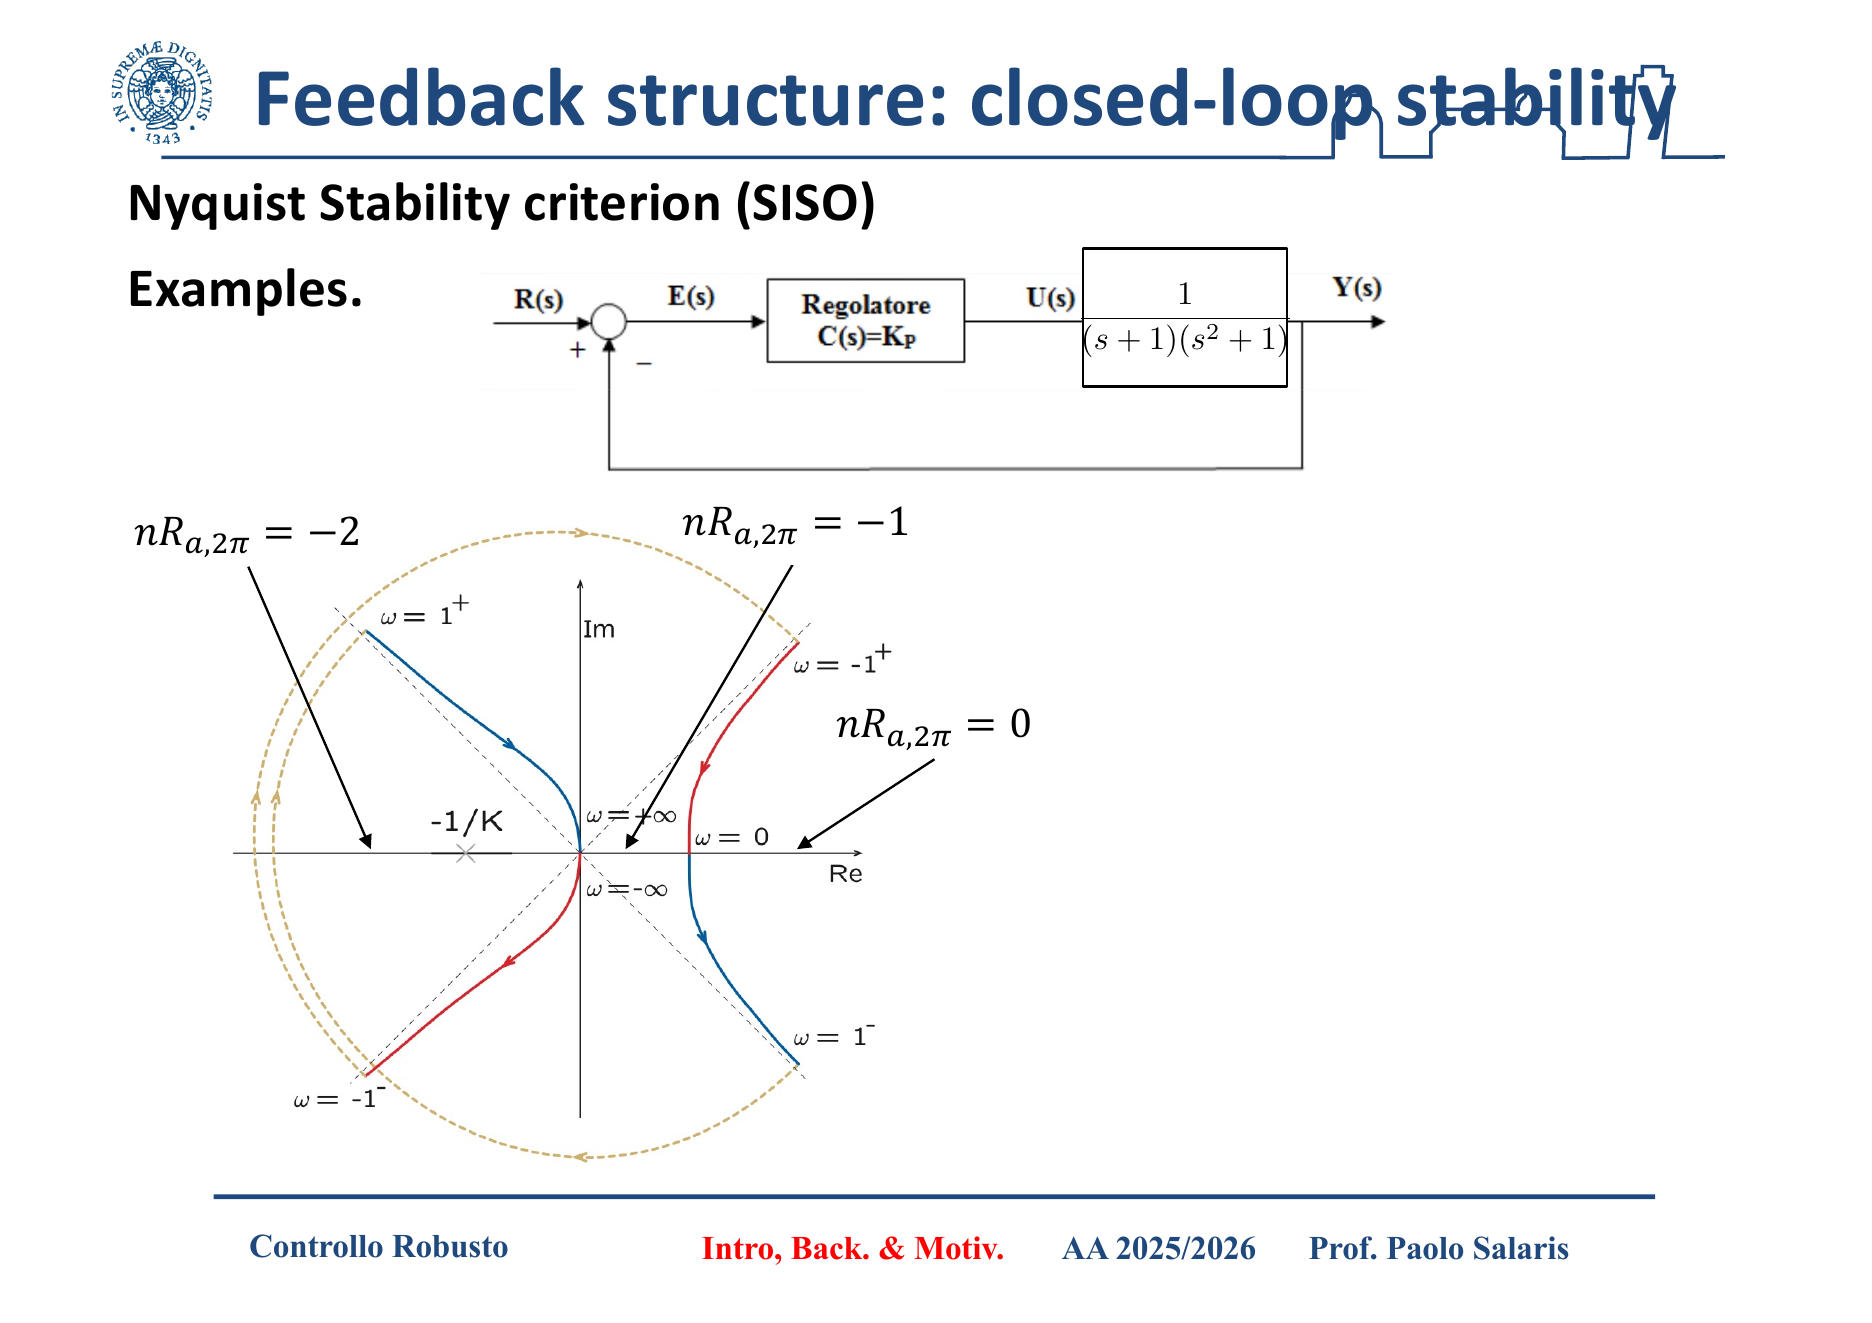
\includegraphics[width=0.70\textwidth]{images/example_1_over_splus1_s2plus1.png}
    \caption{Nyquist con poli su asse immaginario in $\omega=\pm1$. L’interpretazione corretta richiede di considerare i rami che vanno all’infinito.}
    \label{fig:imaginary_poles_example}
\end{figure}

Questo esempio chiarisce una sottigliezza spesso trascurata: il criterio di Nyquist resta applicabile, ma non nella forma ingenua di semplice sostituzione $s=j\omega$ senza deformazioni del contorno.

\subsubsection{Esempio con zeri immaginari: \texorpdfstring{$\boldsymbol{(s^2+100)/(s(s+1)(s+10))}$}{(s squared+100) over s(s+1)(s+10)}}

Con
$$
G(s)=\frac{s^2+100}{s(s+1)(s+10)}
$$
compaiono zeri in $s=\pm 10j$. Gli zeri sull’asse immaginario non generano singolarità del luogo come fanno i poli, ma influenzano la forma della curva rendendo possibile lobi e auto-intersezioni apparenti.

\begin{figure}[H]
    \centering
    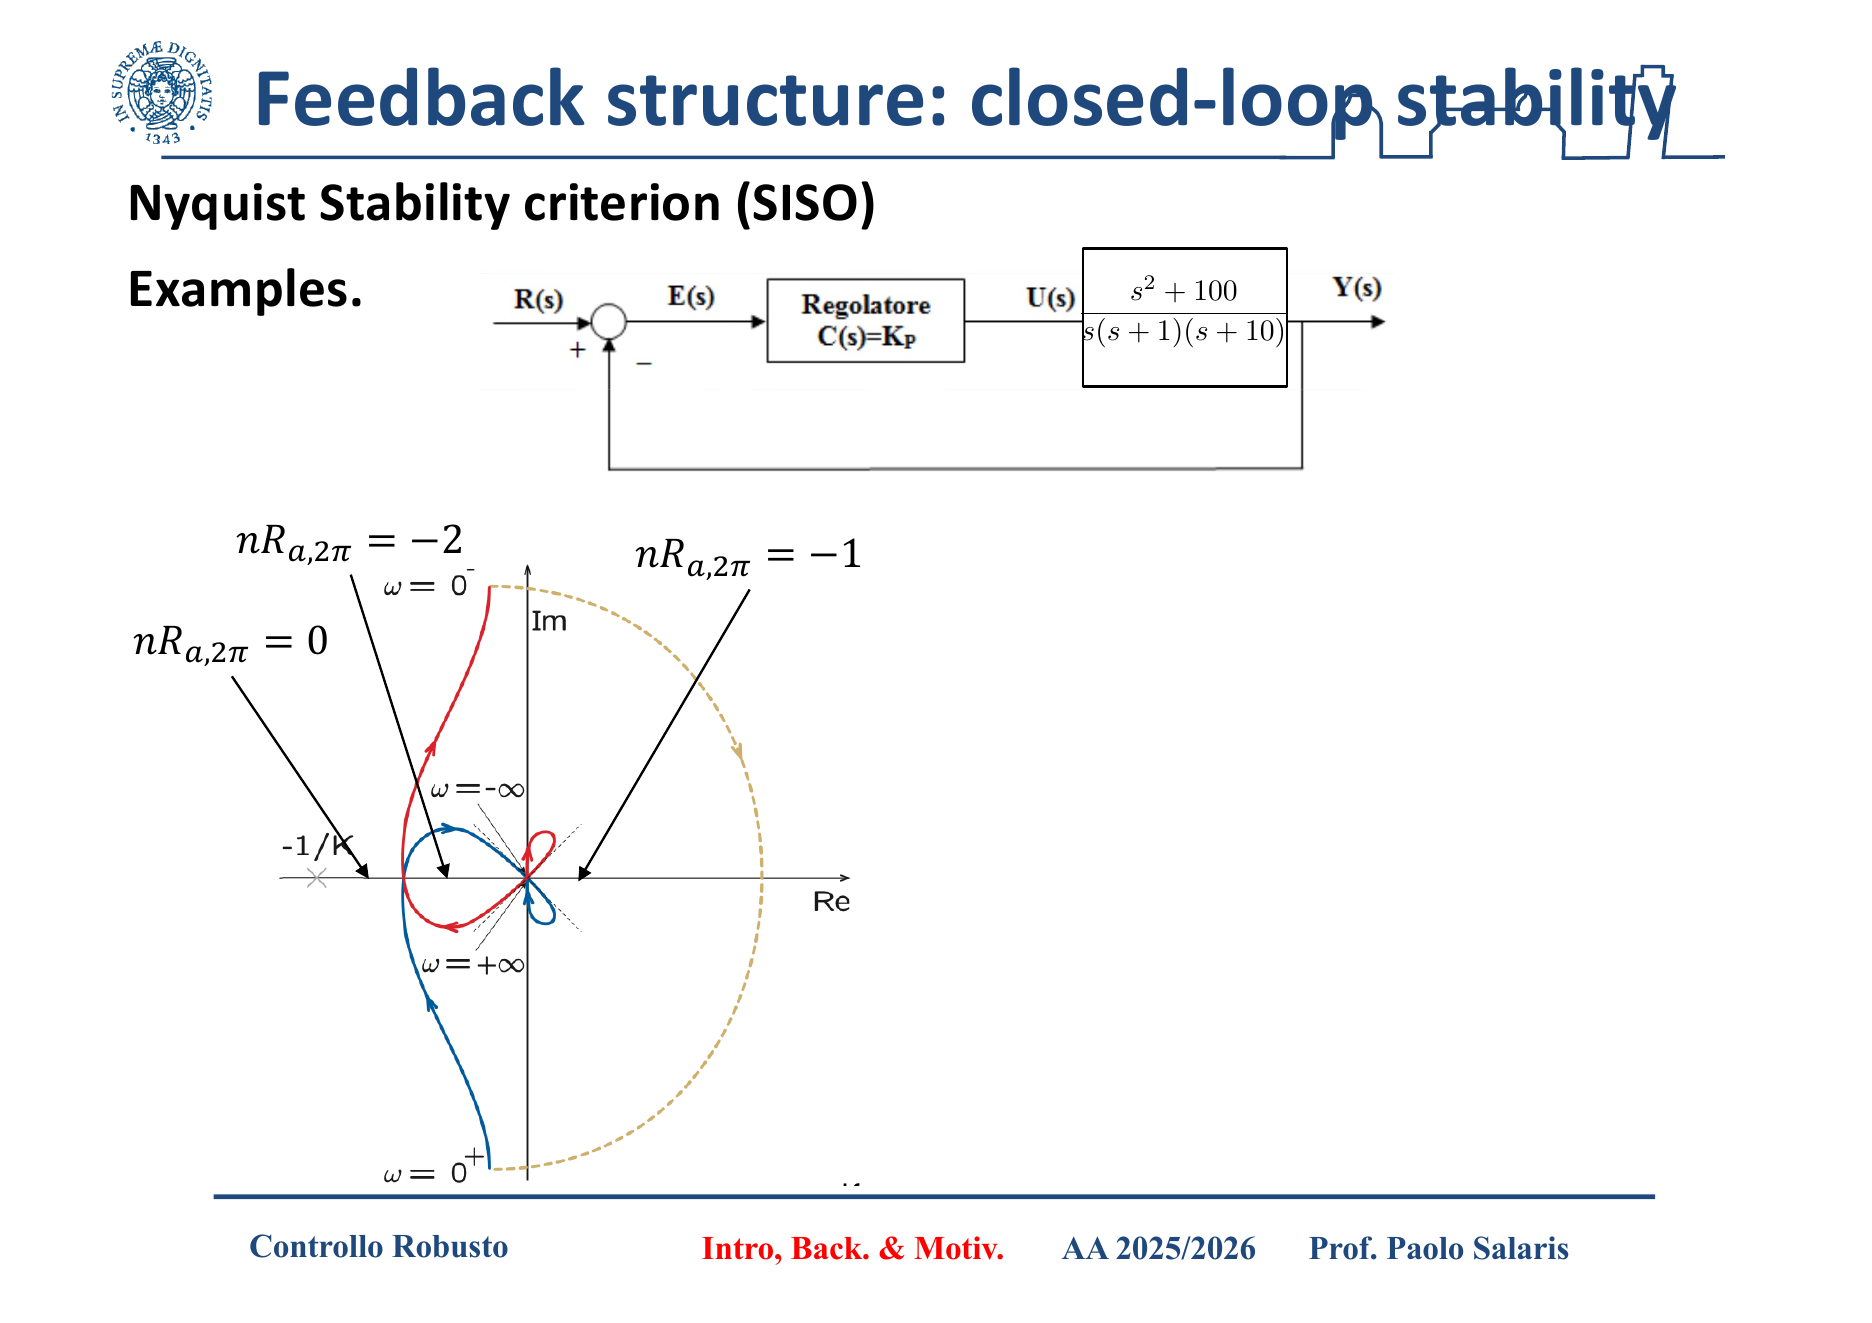
\includegraphics[width=0.68\textwidth]{images/example_s2plus100.png}
    \caption{Esempio in cui gli zeri su asse immaginario modificano la forma del luogo pur non introducendo singolarità del tipo polo.}
    \label{fig:s2plus100}
\end{figure}

Da un punto di vista progettuale, questo tipo di esempio allena a non confondere la presenza di un attraversamento dell’asse reale con un reale cambio di stabilità. Ciò che conta è sempre il numero netto di avvolgimenti del punto critico.

\subsubsection{Esempio con polo instabile esplicito: \texorpdfstring{$\boldsymbol{(s+1)/(s(s/10-1))}$}{(s+1)/(s(s/10-1))}}

La funzione
$$
G(s)=\frac{s+1}{s\left(\frac{s}{10}-1\right)}
$$
ha un polo nell’origine e un polo instabile in $s=10$. Quindi il conteggio teorico richiede di compensare due situazioni delicate: il polo sull’asse immaginario e il polo nel semipiano destro.

\begin{figure}[H]
    \centering
    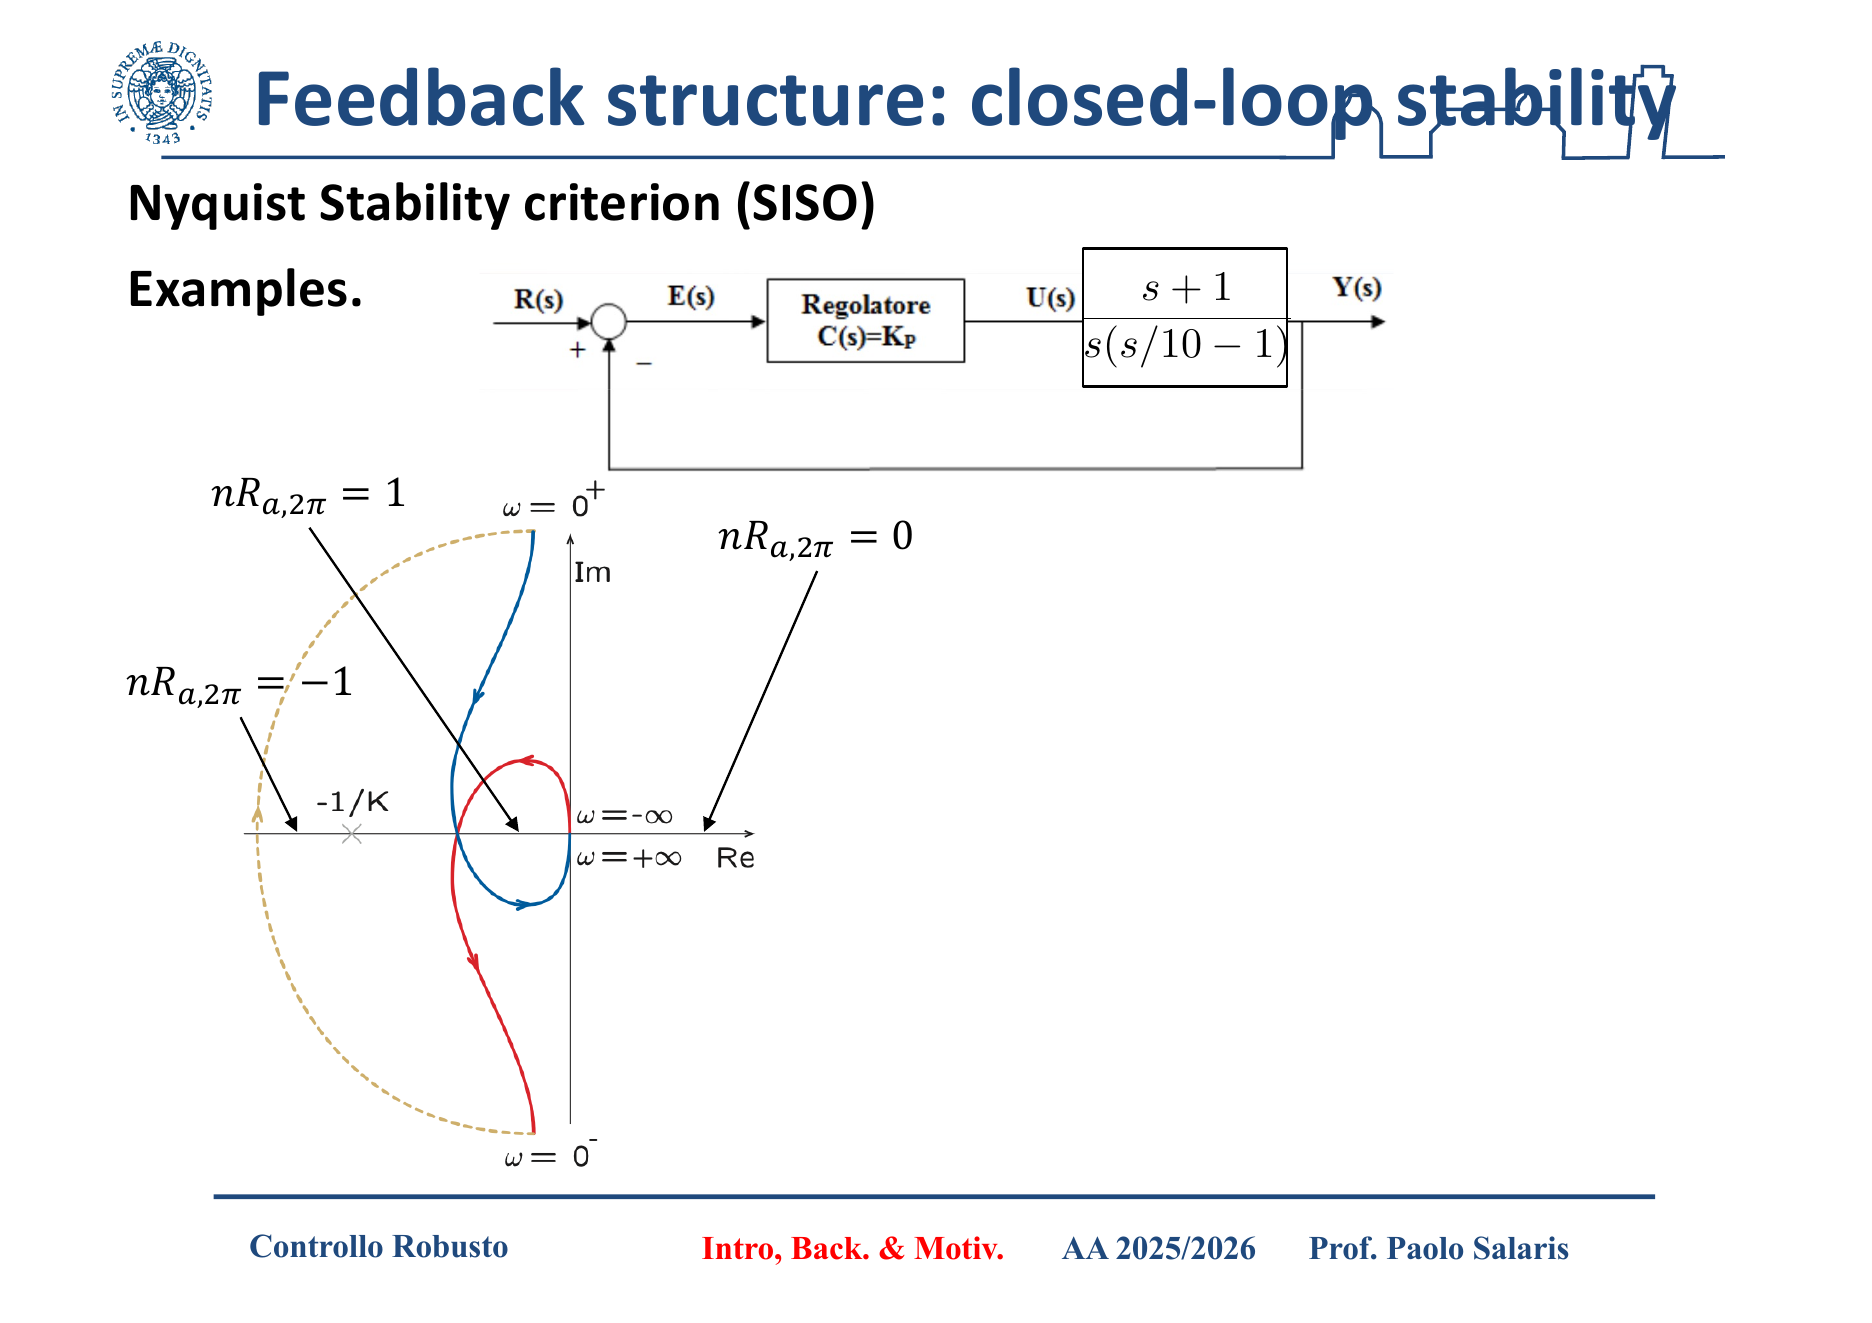
\includegraphics[width=0.68\textwidth]{images/example_splus1_over_s_s10minus.png}
    \caption{Esempio con un integratore e un polo instabile. Il luogo può produrre regioni di guadagno stabili e instabili a seconda della posizione di $-1/K$.}
    \label{fig:unstable_and_integrator}
\end{figure}

Questo tipo di impianto è didatticamente prezioso perché mostra che la sola presenza di un polo instabile in anello aperto non impedisce la stabilizzazione via retroazione: il luogo di Nyquist può comunque generare il numero necessario di avvolgimenti del punto $-1$.

\subsubsection{Confronto fra diversi numeri di integratori}

Un confronto particolarmente significativo è quello fra
$$
G_1(s)=\frac{1}{s(s+1)},
\qquad
G_2(s)=\frac{1}{s^5(s+1)}.
$$

\begin{figure}[H]
    \centering
    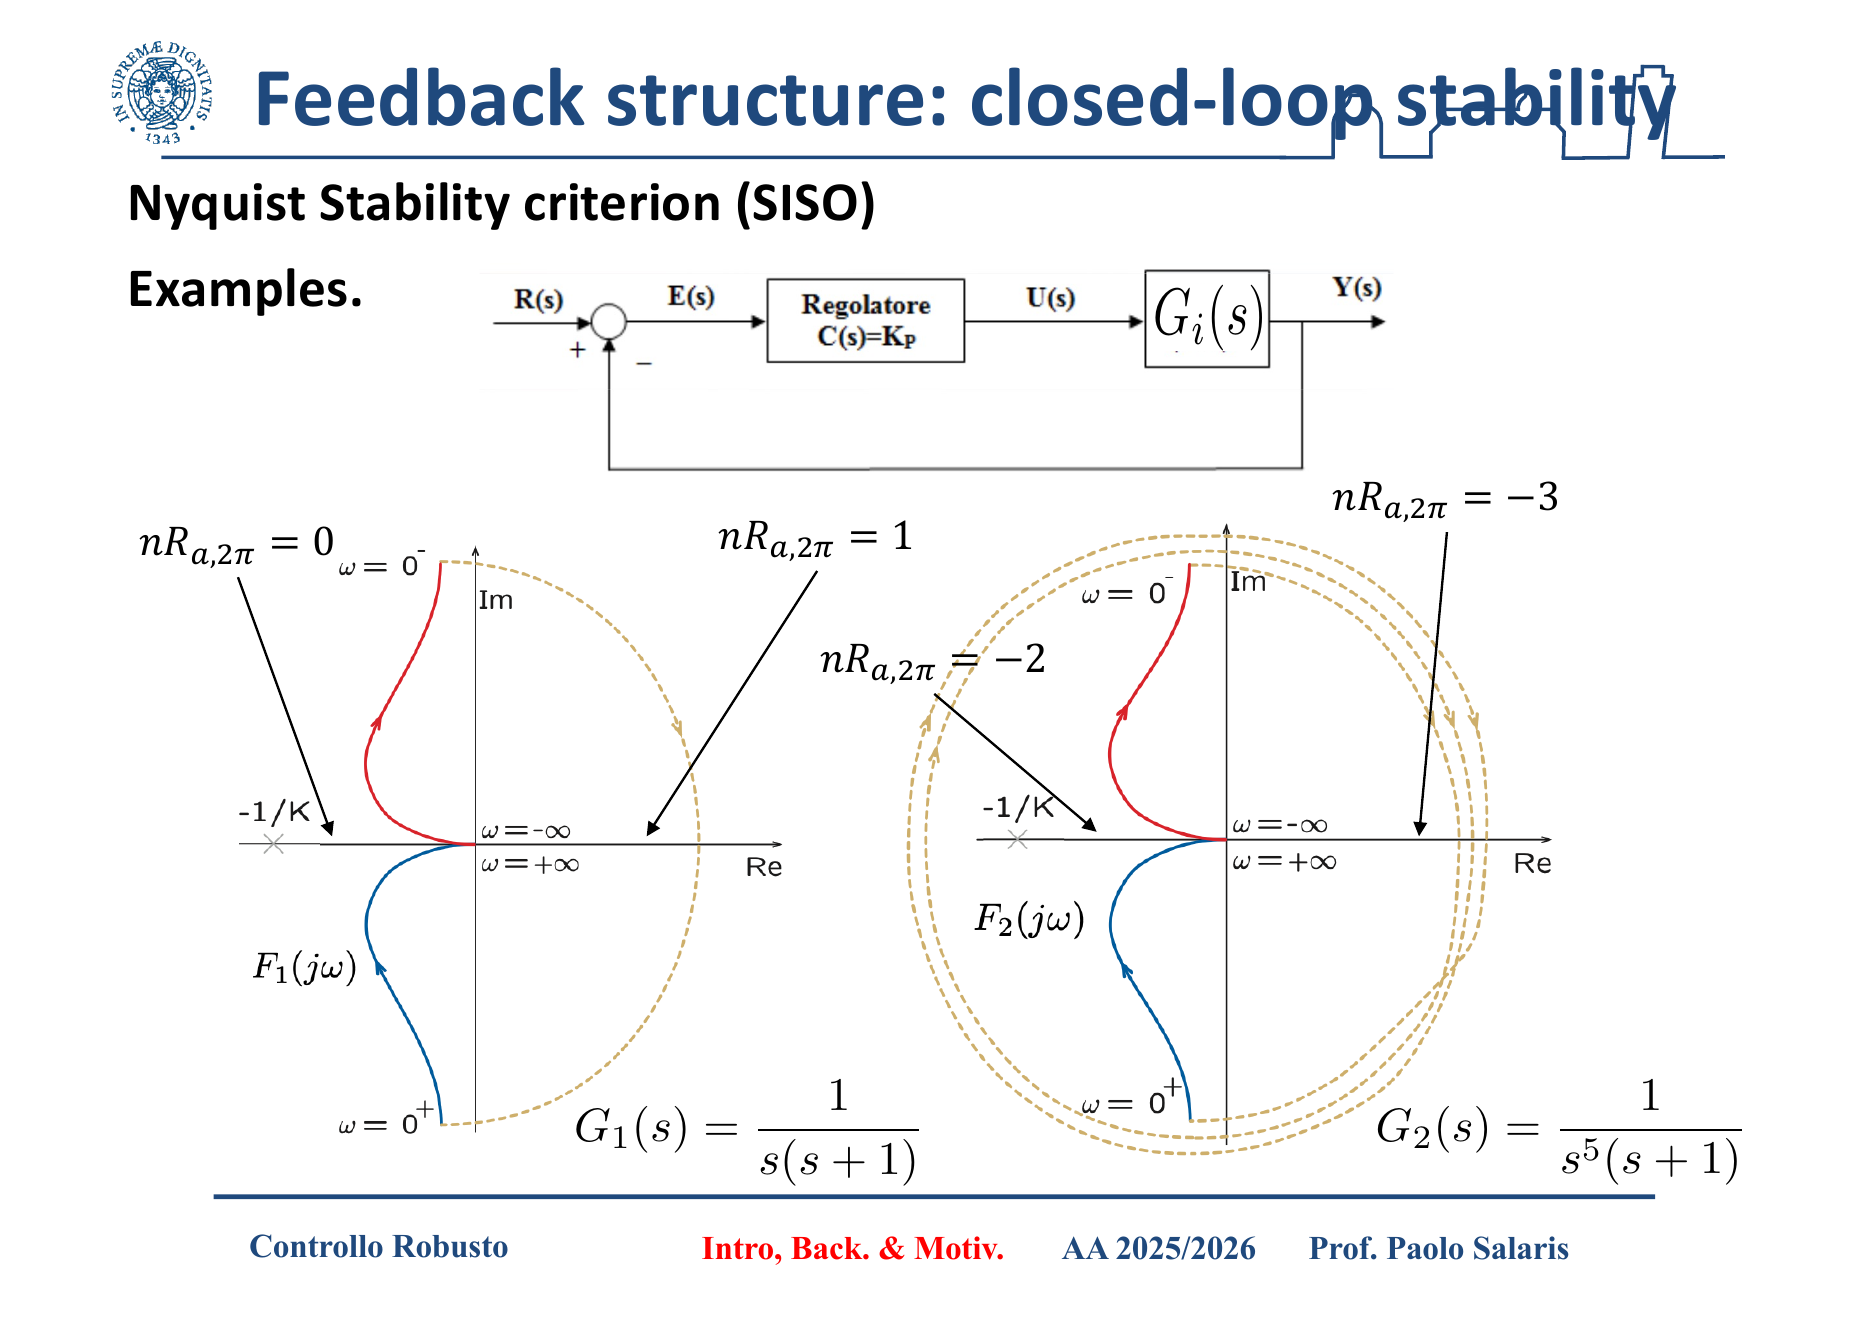
\includegraphics[width=0.9\textwidth]{images/example_integrators.png}
    \caption{Confronto fra un impianto con un solo integratore e una con cinque integratori. L’aumento dell’ordine all’origine cambia drasticamente la topologia del luogo di Nyquist.}
    \label{fig:many_integrators}
\end{figure}

La presenza di più poli nell’origine aumenta il ritardo di fase alle basse frequenze e deforma il luogo in modo crescente. Dal punto di vista del margine di stabilità, molti integratori tendono a rendere il sistema più delicato, perché il luogo si dispone in prossimità del punto critico con angoli e curvature meno favorevoli.

\subsection{Osservazioni metodologiche per applicare bene Nyquist}

Dopo gli esempi, conviene fissare una procedura operativa standard.

\begin{enumerate}
    \item Si individuano i poli di anello aperto nel semipiano destro e sull’asse immaginario.
    \item Si costruisce o si interpreta il luogo di Nyquist completo, includendo eventuali simmetrie e chiusure all’infinito.
    \item Si sceglie una convenzione coerente per il verso di percorrenza e per il conteggio degli avvolgimenti.
    \item Si conta il numero netto di avvolgimenti del punto critico $-1$.
    \item Si verifica se il conteggio ottenuto è compatibile con il numero di poli instabili dell’anello aperto.
\end{enumerate}

Gli errori più frequenti sono tre. Il primo è ignorare la parte a frequenze negative, dimenticando la simmetria. Il secondo è dimenticare le deviazioni attorno ai poli sull’asse immaginario. Il terzo è contare semplicemente quante volte il luogo \emph{passa vicino} a $-1$ invece di contare gli avvolgimenti netti con orientazione.

\subsection{Generalized Nyquist Stability Criterion nel caso MIMO}
\label{sec:mimo}

Passiamo ora al caso multi-variabile. Sia $P(s)$ una matrice di trasferimento quadrata e razionale, e sia $K_c(s)$ il controllore. La funzione di trasferimento in anello chiuso può essere scritta come
$$
G_c(s)=P(s)K_c(s)\left(I+P(s)K_c(s)\right)^{-1}.
$$

I poli dell’anello chiuso sono le radici della condizione
$$
\det\bigl(I+P(s)K_c(s)\bigr)=0.
\label{eq:mimo_char}
$$

\begin{figure}[H]
    \centering
    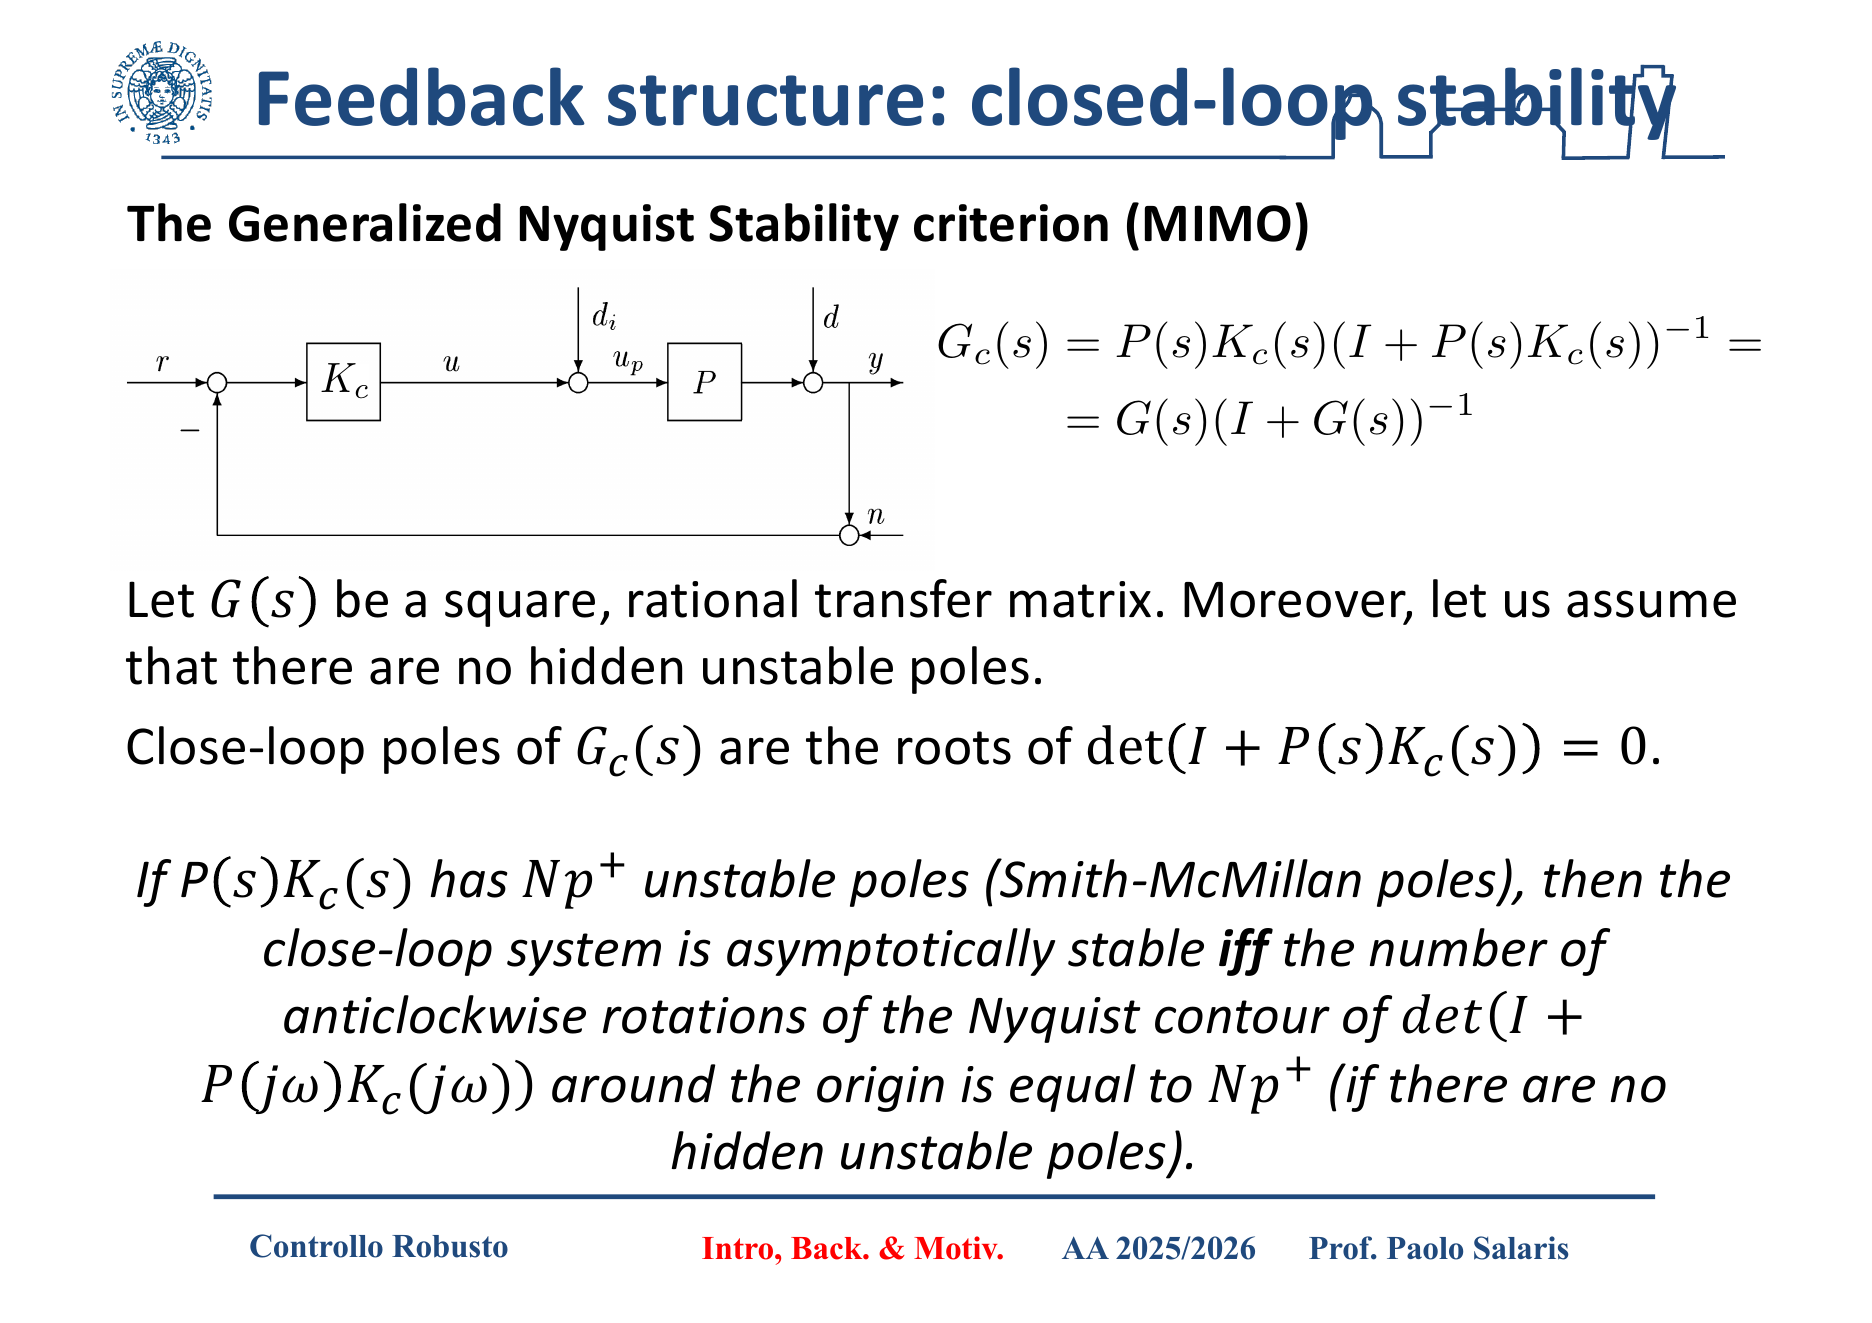
\includegraphics[width=0.86\textwidth]{images/generalized_nyquist_intro.png}
    \caption{Slide introduttiva al criterio di Nyquist generalizzato: nel caso MIMO l’oggetto chiave è il determinante di $I+P(s)K_c(s)$.}
    \label{fig:generalized_intro}
\end{figure}

Il parallelo con il caso SISO è immediato. Nel caso SISO l’equazione caratteristica è $1+G(s)=0$; nel caso MIMO diventa il determinante della matrice di ritorno. Se $P(s)K_c(s)$ ha $N_p^+$ poli instabili in senso Smith--McMillan e non ci sono modi instabili nascosti, allora il sistema chiuso è asintoticamente stabile se e solo se il luogo di Nyquist di
$$
\det\bigl(I+P(j\omega)K_c(j\omega)\bigr)
$$
compie il numero corretto di avvolgimenti dell’origine.

\subsubsection{Perché compare il determinante}

Il determinante compare perché una matrice è singolare esattamente quando il suo determinante è nullo. Dato che l’anello chiuso perde invertibilità quando $I+P(s)K_c(s)$ diventa singolare, \eqref{eq:mimo_char} è la naturale generalizzazione dell’equazione $1+G(s)=0$.

Tuttavia c’è una differenza profonda rispetto al caso SISO: la quantità
$$
\det(I+kP(s))
$$
non dipende linearmente dal guadagno $k$. Questo rende la lettura geometrica meno immediata.

\subsubsection{Esempio di non linearità nel guadagno}

Per un impianto $2\times 2$ con controllore diagonale
$$
P(s)=\begin{bmatrix}P_{11} & P_{12}\\ P_{21} & P_{22}\end{bmatrix},
\qquad
K(s)=\begin{bmatrix}K_1 & 0\\ 0 & K_2\end{bmatrix},
$$
si ha
\begin{align*}
\det(I+P(s)K(s))
&=\det\begin{bmatrix}1+K_1P_{11} & K_2P_{12}\\ K_1P_{21} & 1+K_2P_{22}\end{bmatrix} \\
&=(1+K_1P_{11})(1+K_2P_{22})-K_1K_2P_{21}P_{12}.
\end{align*}

Se inoltre $K_1=K_2=K$, allora
$$
\det(I+KP(s)) = 1 + K(P_{11}+P_{22}) + K^2(P_{11}P_{22}-P_{12}P_{21}),
$$
che è chiaramente non lineare in $K$. Questo spiega perché nel caso MIMO non basta spostare il punto critico lungo l’asse reale come nel caso SISO.

\subsection{Characteristic loci e autovalori di \texorpdfstring{$P(s)$}{P(s)}}

Il modo elegante per recuperare la potenza del criterio classico è passare agli autovalori di $P(s)$. Se $\lambda_i(s)$ è un autovalore di $P(s)$, allora $k\lambda_i(s)$ è un autovalore di $kP(s)$, mentre $1+k\lambda_i(s)$ è un autovalore di $I+kP(s)$. Poiché il determinante è il prodotto degli autovalori, segue che
$$
\det(I+kP(s)) = \prod_i \bigl(1+k\lambda_i(s)\bigr).
\label{eq:det_prod_eigs}
$$

Applicando il logaritmo dell’argomento al prodotto, si ottiene
$$
\Delta \operatorname{Arg} \det(I+kP(s)) = \sum_i \Delta \operatorname{Arg}\bigl(1+k\lambda_i(s)\bigr).
$$

Questo significa che, invece di tracciare il luogo del determinante per ogni $k$, possiamo tracciare una sola volta i luoghi degli autovalori $\lambda_i(j\omega)$, detti \emph{characteristic loci}, e contare collettivamente i loro avvolgimenti del punto $-1/k$.

\begin{keybox}
Nel caso MIMO il criterio di Nyquist si applica non a una singola curva, ma all’insieme dei luoghi degli autovalori della matrice di trasferimento. La somma degli avvolgimenti di tutti i rami deve compensare il numero di poli instabili di $P(s)$.
\end{keybox}

\subsection{Esempio MIMO con autovalori espliciti}

Le slide propongono il sistema
$$
P(s)=\begin{bmatrix}
0 & 1\\
\dfrac{s-1}{s+1} & 0
\end{bmatrix}.
$$

Gli autovalori sono
$$
\lambda_i(s)=\pm \sqrt{\frac{s-1}{s+1}}.
$$

\begin{figure}[H]
    \centering
    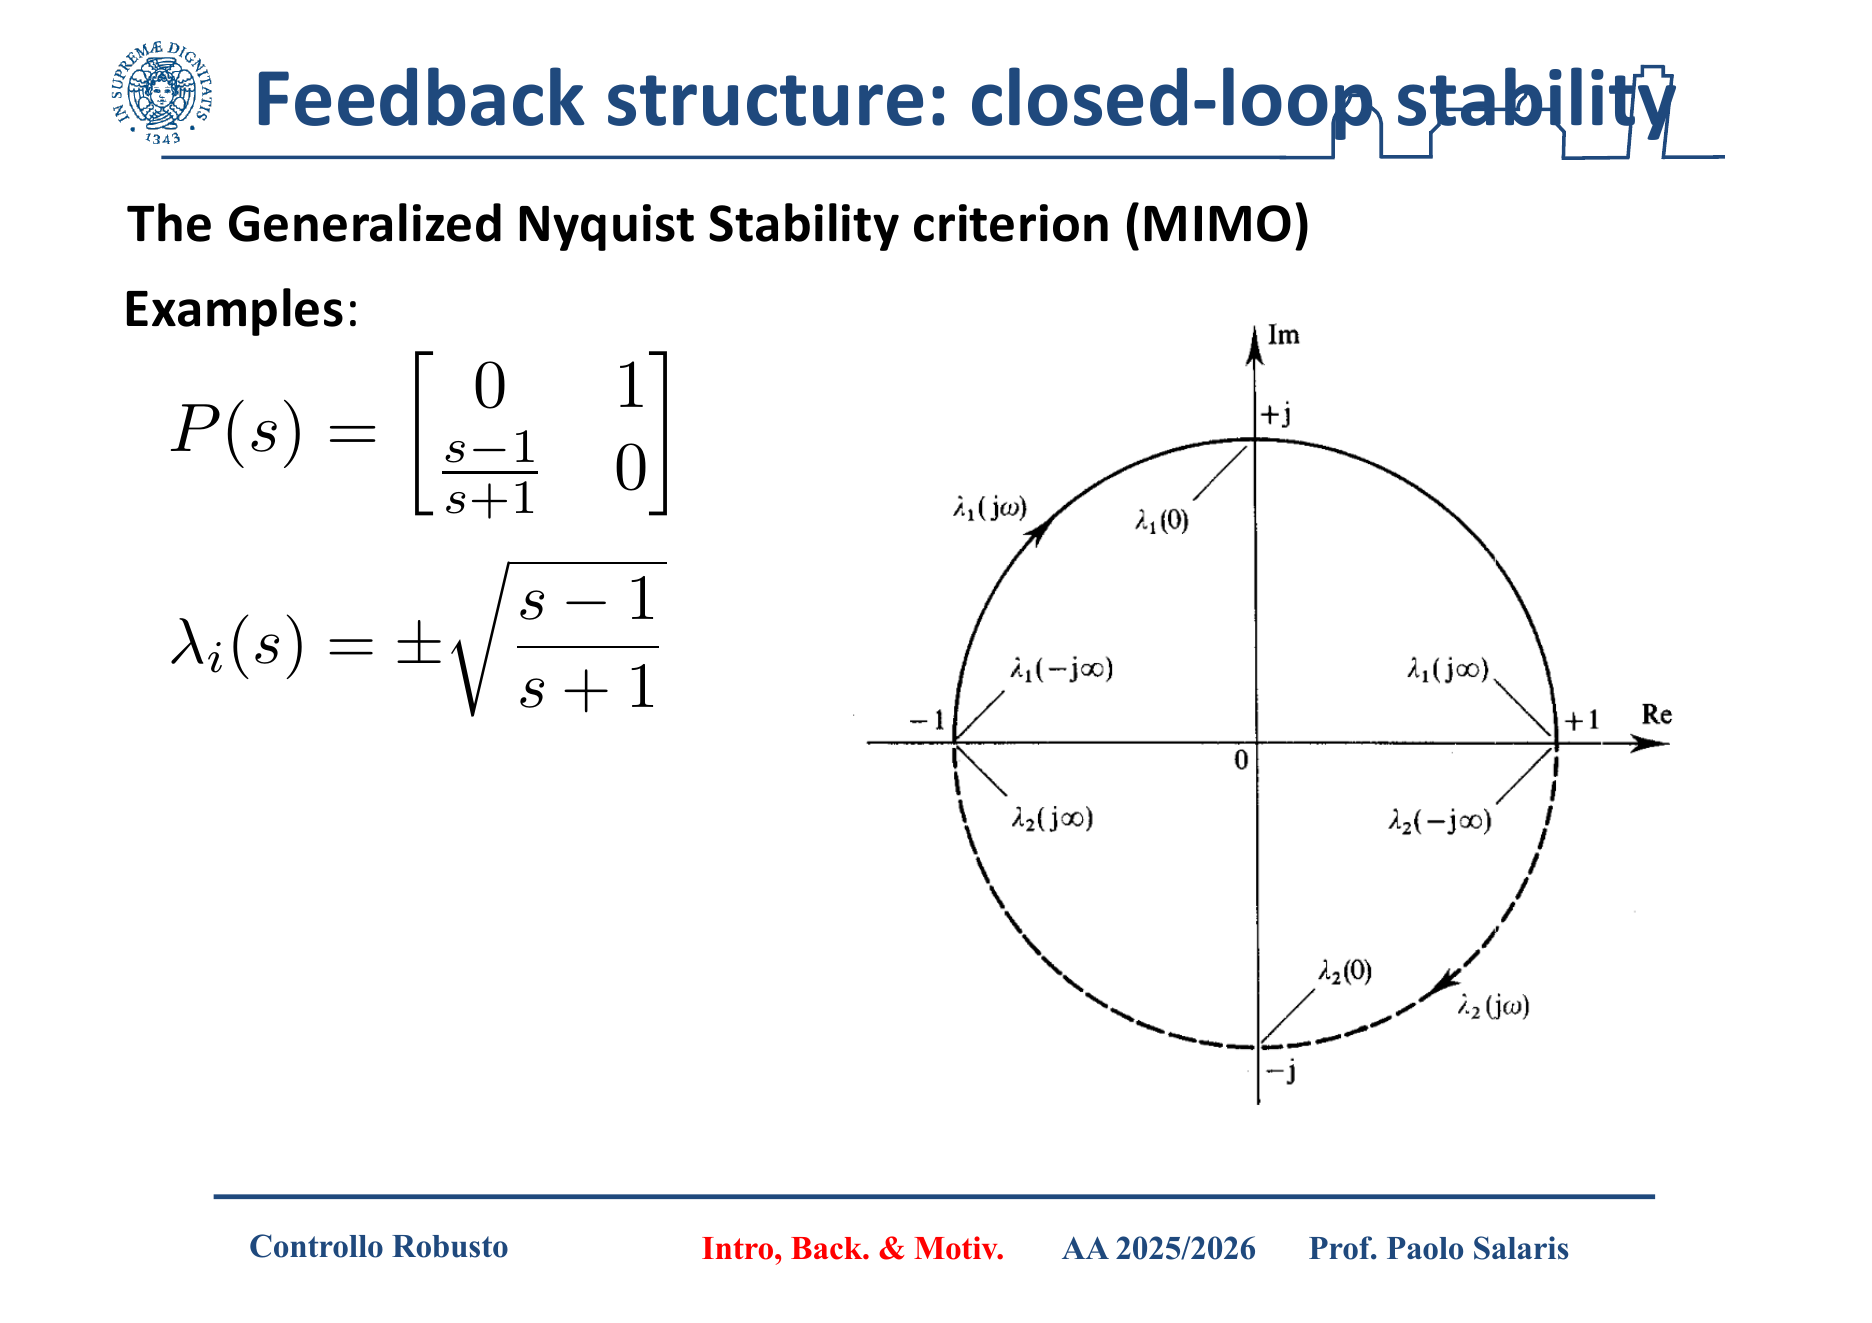
\includegraphics[width=0.72\textwidth]{images/mimo_characteristic_loci.png}
    \caption{Characteristic loci di un sistema MIMO. I due rami corrispondono ai due autovalori della matrice di trasferimento.}
    \label{fig:mimo_char_loci}
\end{figure}

Questo esempio è illuminante per due ragioni. Primo, mostra che i characteristic loci possono vivere su curve non banali e non necessariamente simmetriche come nel caso SISO. Secondo, chiarisce che il criterio non si applica a ciascun ramo in modo indipendente, ma alla somma complessiva degli avvolgimenti di tutti i rami.

Dal punto di vista intuitivo, ogni autovalore descrive una ``direzione modale'' della dinamica MIMO. La stabilità del sistema chiuso dipende quindi da come tutte queste direzioni interagiscono con il punto critico.

\subsection{Esempio MIMO con regioni di stabilità in funzione del guadagno}

Un altro esempio delle slide considera un impianto del tipo
$$
P(s)=\frac{1}{1.25(s+1)(s+2)}
\begin{bmatrix}
s-1 & s\\
-6 & s-2
\end{bmatrix}.
$$

La slide evidenzia diversi valori del parametro $-1/k$ per i quali il numero di avvolgimenti cambia. In particolare vengono mostrate regioni di guadagno che producono assenza di avvolgimenti e quindi stabilità in anello chiuso, dato che in questo esempio l'impianto non possiede poli instabili.

\begin{figure}[H]
    \centering
    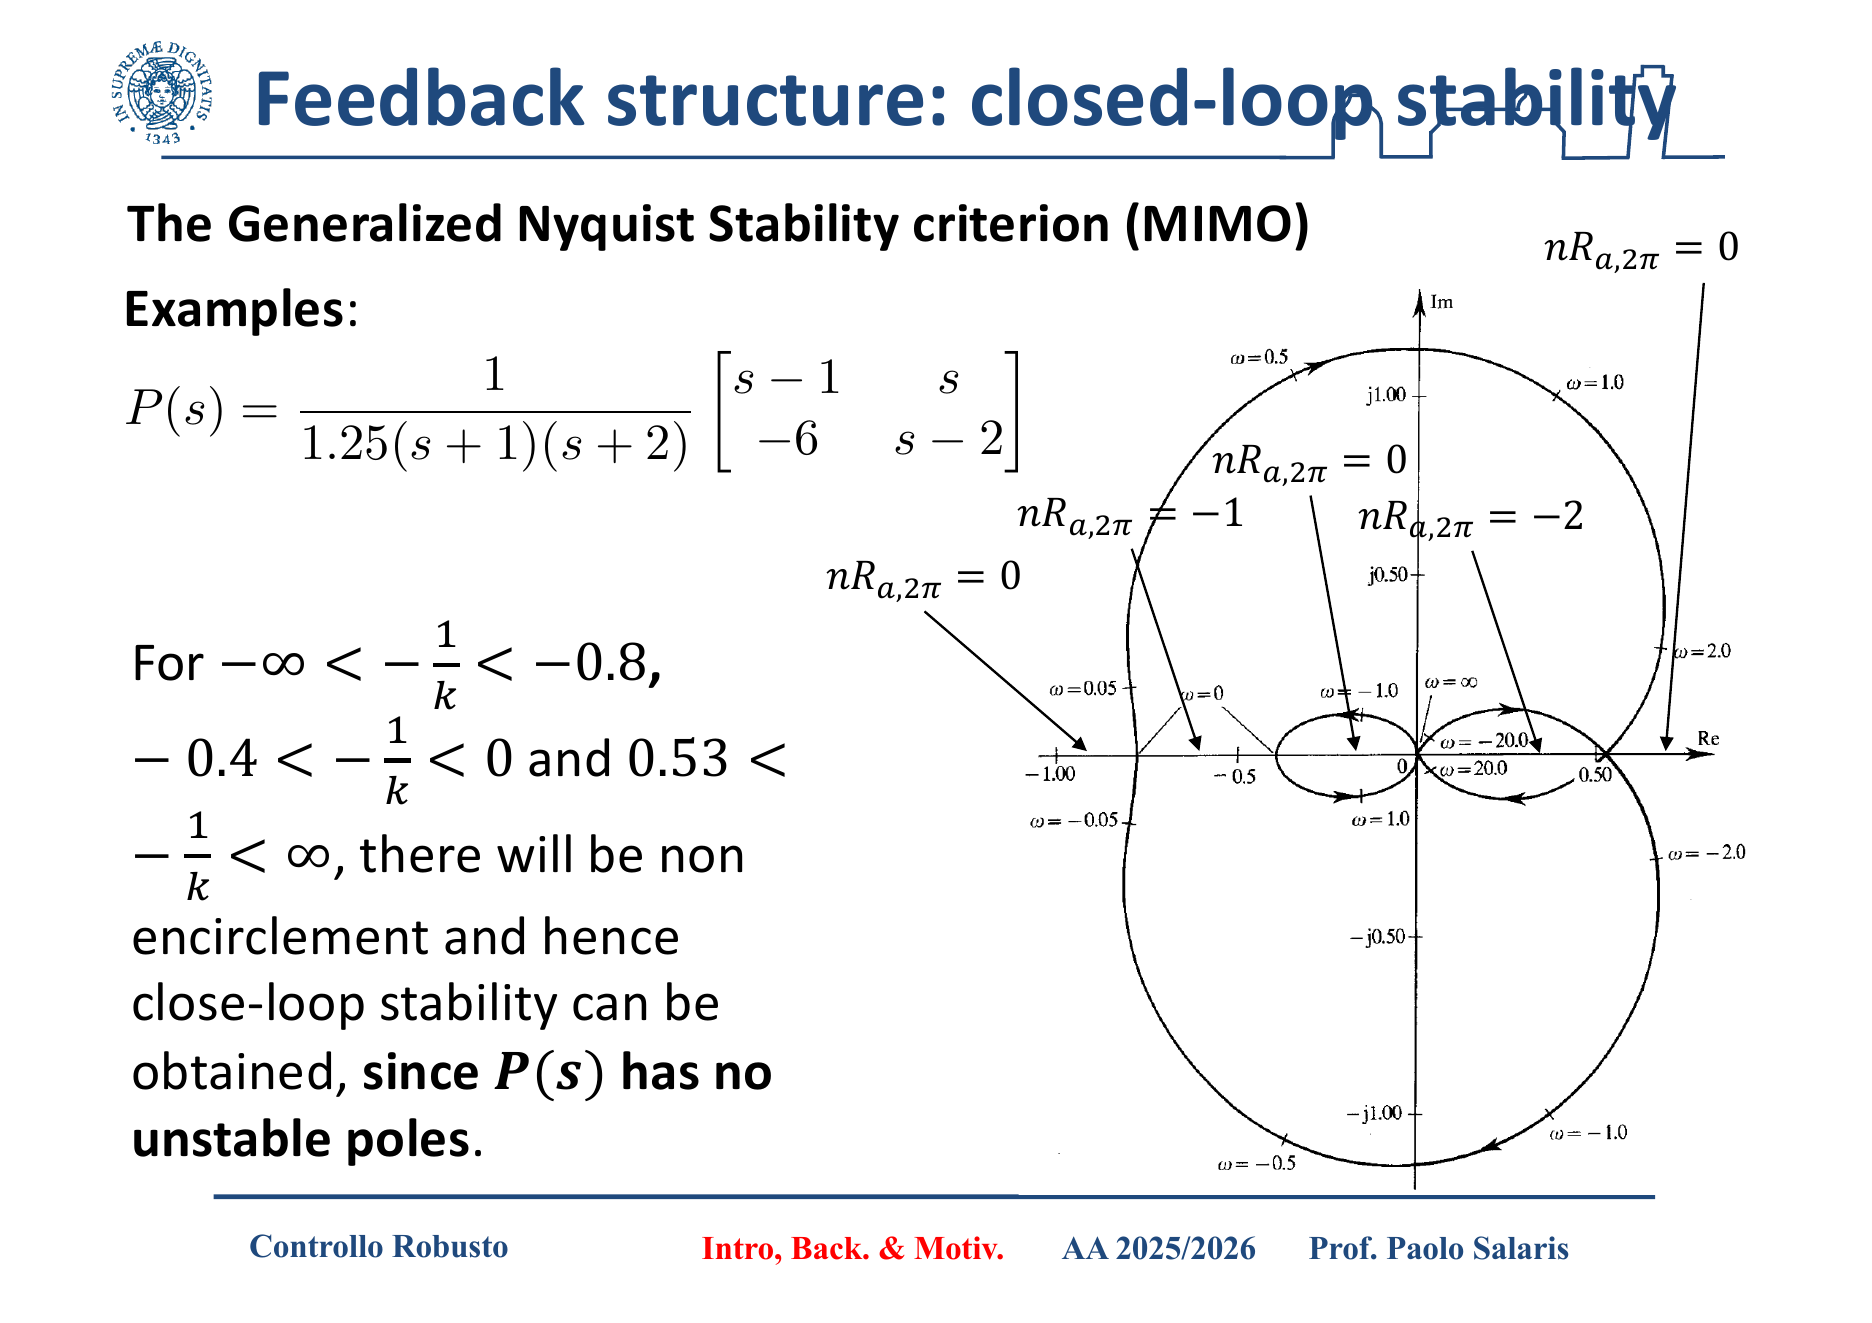
\includegraphics[width=0.78\textwidth]{images/mimo_example_ranges.png}
    \caption{Esempio MIMO in cui la stabilità dipende dalla posizione del punto $-1/k$ rispetto ai characteristic loci.}
    \label{fig:mimo_ranges}
\end{figure}

L’insegnamento operativo è molto simile a quello del caso SISO, ma con una difficoltà in più: il punto critico va confrontato simultaneamente con più rami. In termini di progetto, questo significa che un singolo guadagno scalare può stabilizzare alcune direzioni modali e destabilizzarne altre, se scelto in modo scorretto.

\subsection{Stabilità interna}
\label{sec:internal}

Il capitolo si conclude con un tema fondamentale: non basta che la mappa fra riferimento e uscita sia stabile; tutte le mappe interne del sistema devono essere stabili. Le slide definiscono la stabilità interna nel modo seguente:
\begin{quote}
Un sistema di controllo è internamente stabile se segnali limitati immessi in qualunque punto della struttura generano risposte limitate in qualunque altro punto.
\end{quote}

Per sistemi LTI, questo equivale a richiedere che la funzione di trasferimento fra ogni coppia di segnali interni abbia tutti i poli nel semipiano sinistro aperto.

\begin{figure}[H]
    \centering
    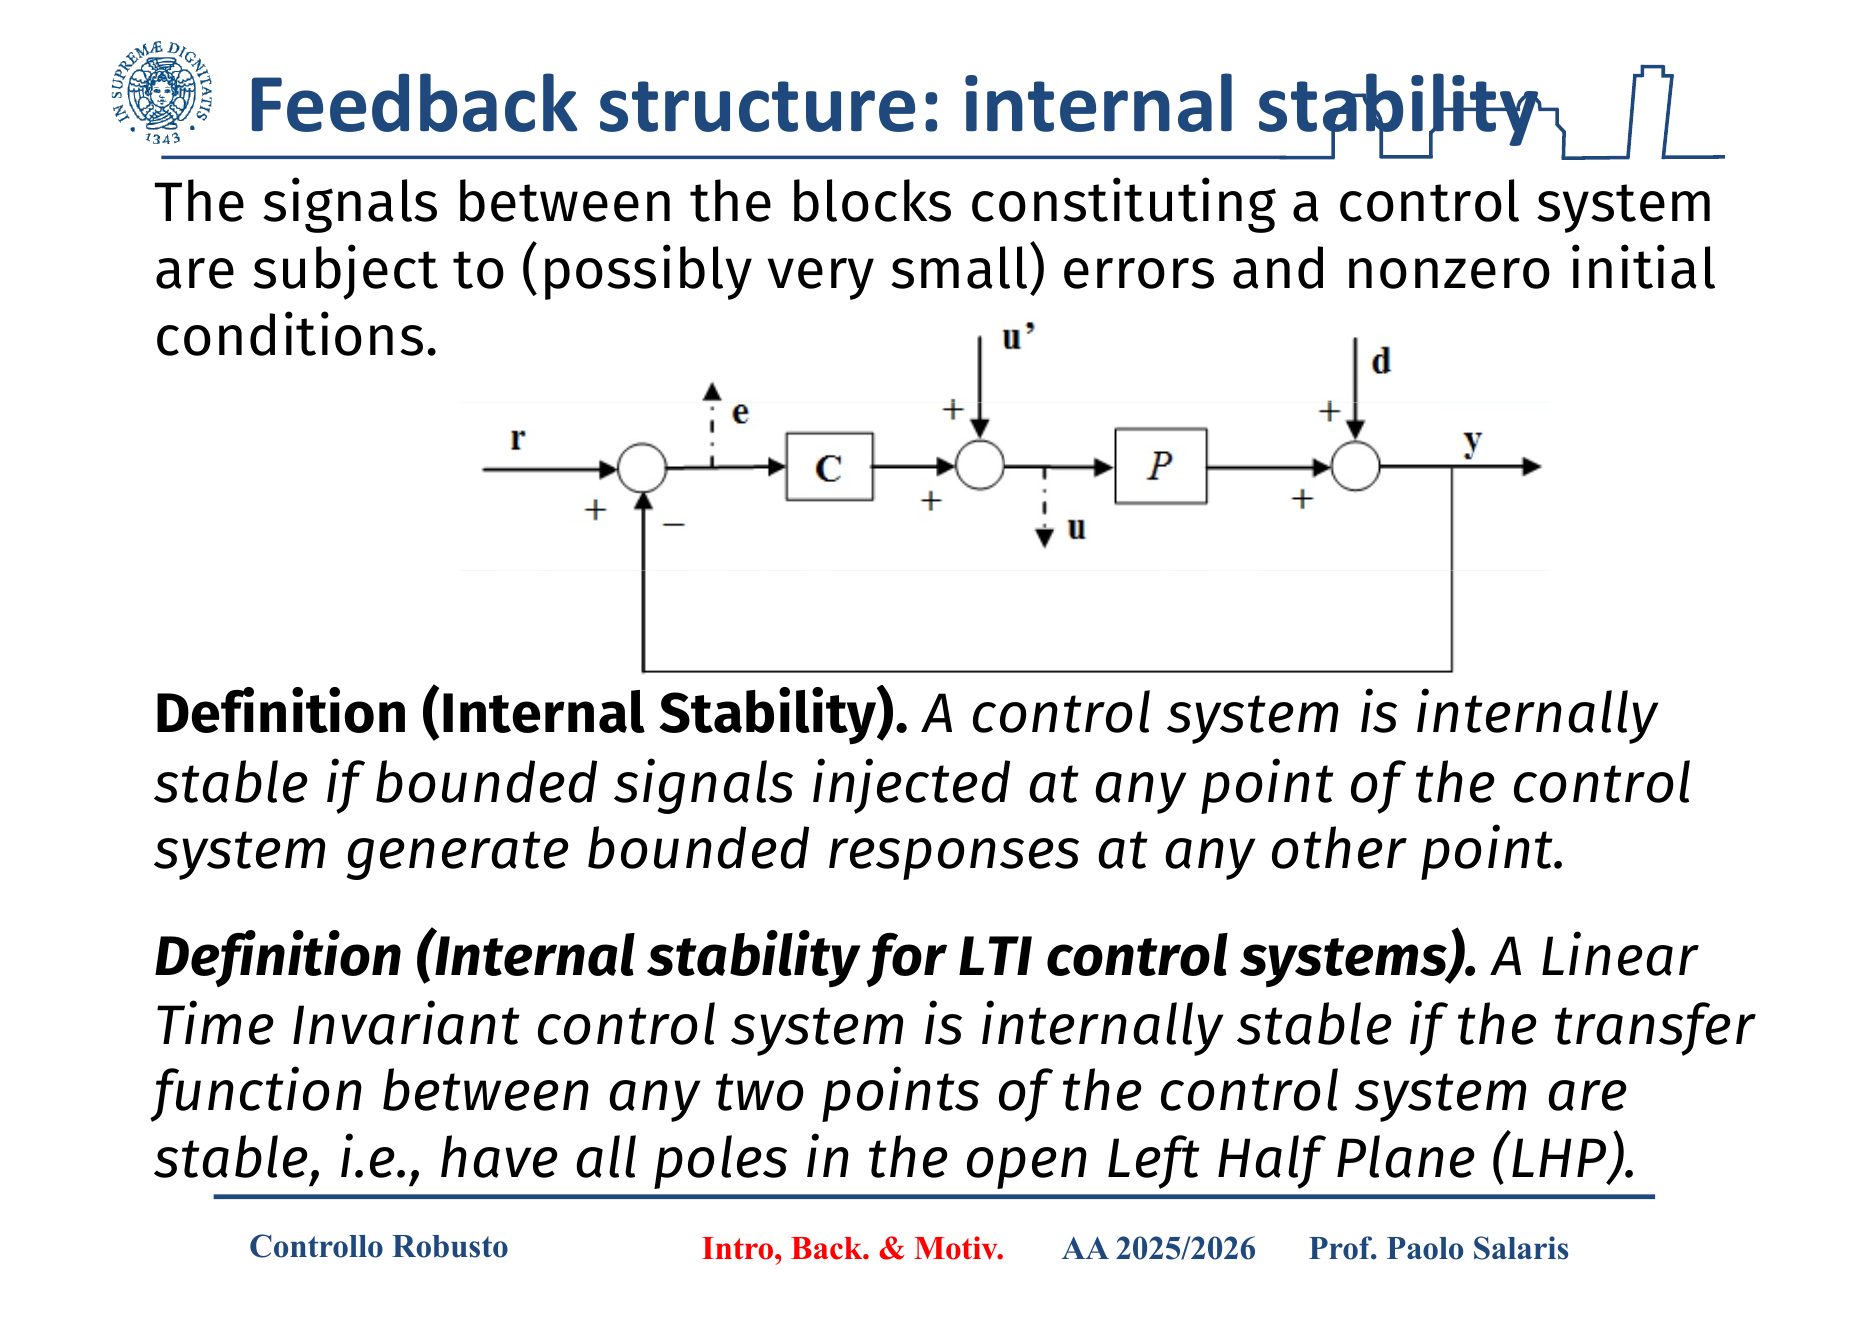
\includegraphics[width=0.83\textwidth]{images/internal_stability_def.png}
    \caption{Definizione di stabilità interna per una struttura di retroazione con ingressi perturbativi in diversi nodi.}
    \label{fig:internal_stability_def}
\end{figure}

Per capire perché questa nozione sia più forte della semplice stabilità input-output, considera che in una struttura con cancellazioni tra poli e zeri può accadere che la funzione di trasferimento esterna sembri stabile, mentre uno stato interno diverge. In controllo robusto questo è inaccettabile, perché piccole incertezze modellistiche rompono la cancellazione esatta e fanno emergere l’instabilità nascosta.

\subsubsection{Matrice delle funzioni di trasferimento interne}

Le slide mostrano che, per la classica struttura con impianto $P$ e controllore $C$, i segnali interni $y$, $u$ ed $e$ possono essere espressi in funzione degli ingressi esterni $r$, $u'$ e $d$ tramite una matrice di trasferimento le cui voci sono tutte combinazioni di $P$, $C$ e del denominatore $1+PC$.

Le forme più note sono
$$
S(s)=\frac{1}{1+P(s)C(s)},
\qquad
T(s)=\frac{P(s)C(s)}{1+P(s)C(s)},
$$
insieme ai termini
$$
\frac{P}{1+PC}, \qquad \frac{C}{1+PC}, \qquad -\frac{CP}{1+PC}, \qquad -\frac{C}{1+PC}, \qquad -\frac{P}{1+PC}.
$$

\begin{figure}[H]
    \centering
    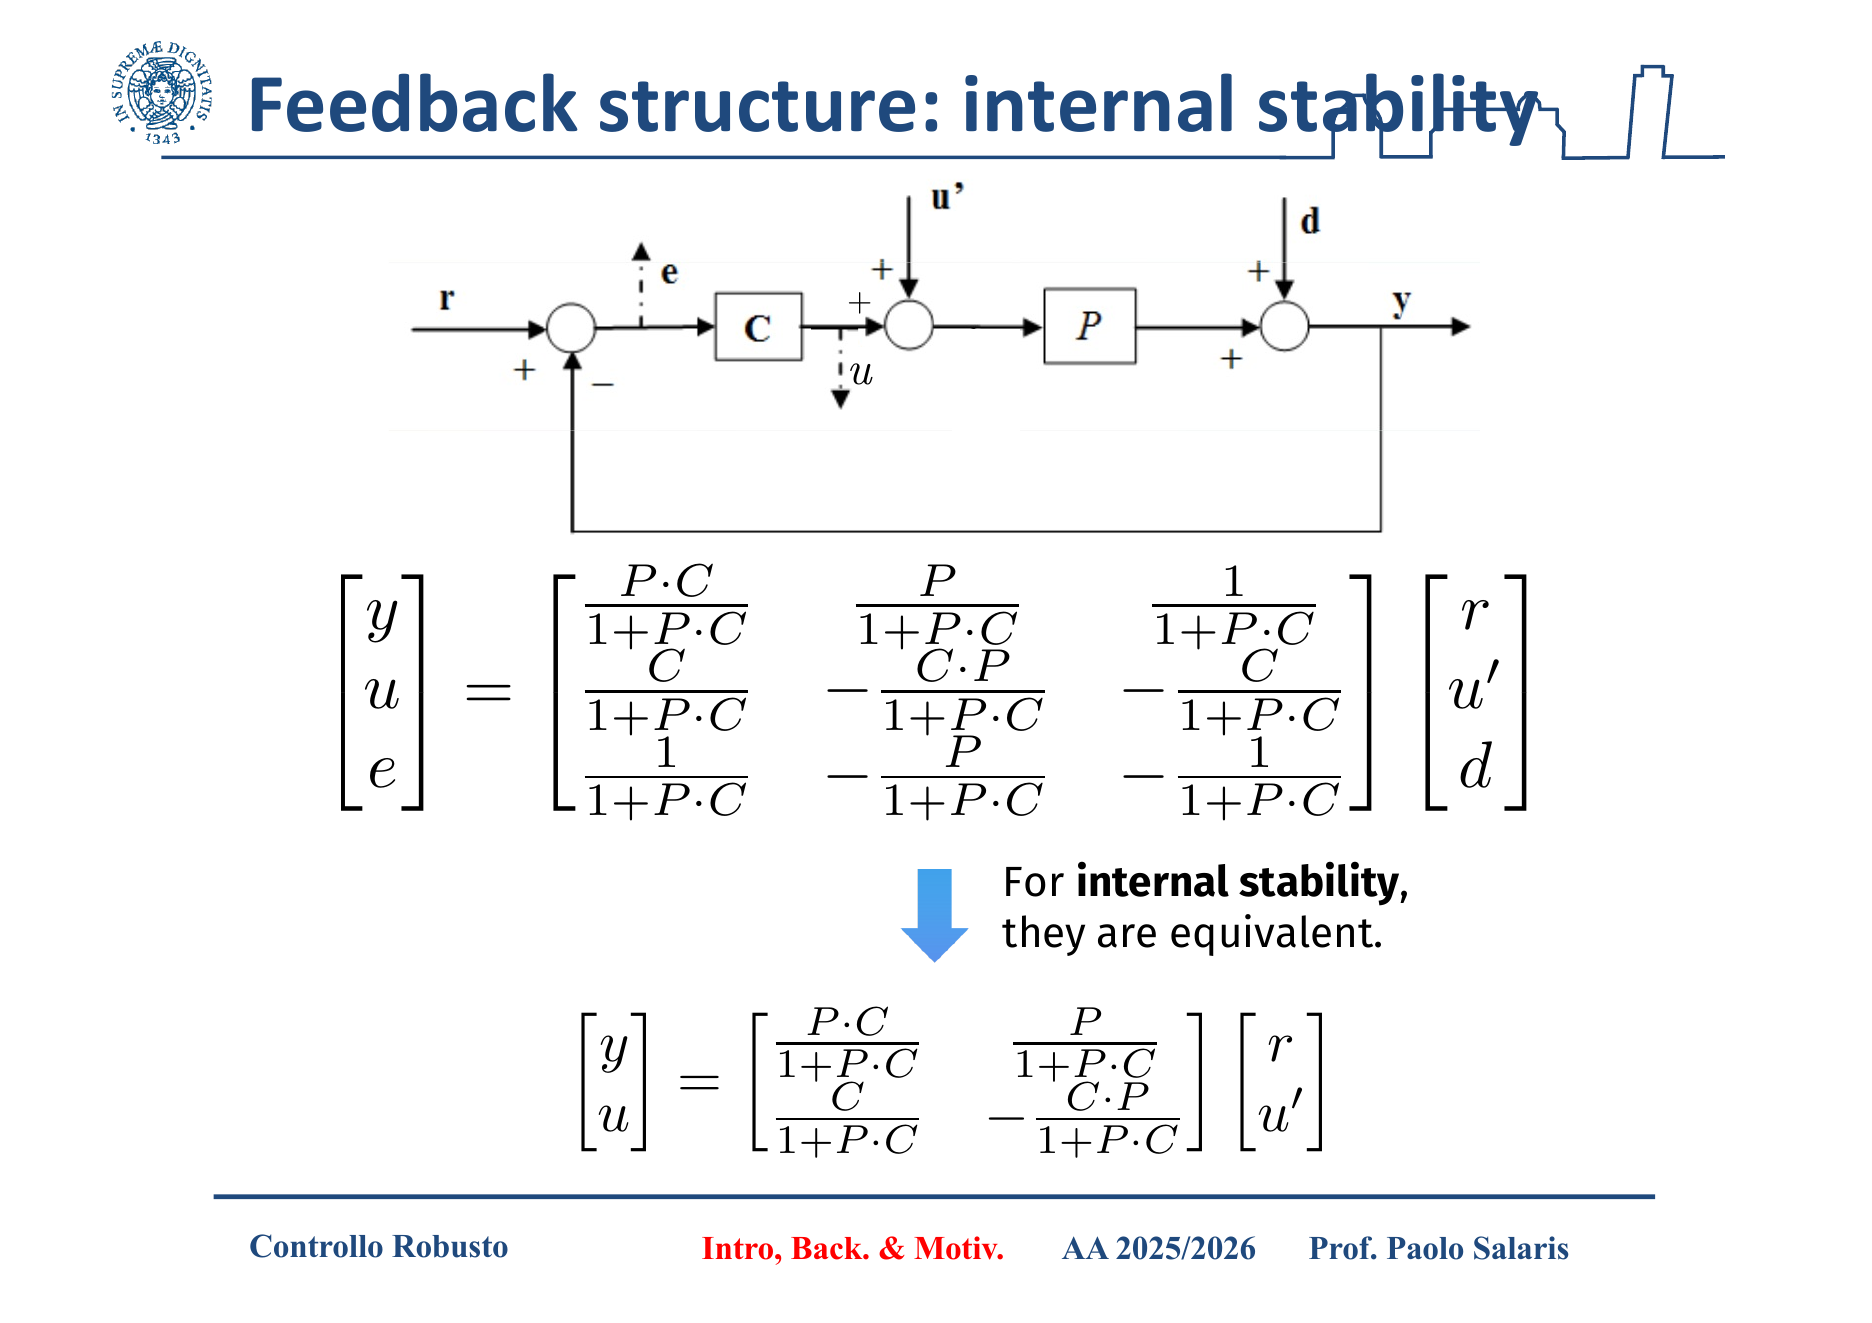
\includegraphics[width=0.82\textwidth]{images/internal_stability_matrix.png}
    \caption{Matrice delle funzioni di trasferimento fra ingressi esterni e segnali interni. La stabilità interna richiede stabilità di tutte queste mappe.}
    \label{fig:internal_matrix}
\end{figure}

L’osservazione decisiva è che tutte queste funzioni hanno lo stesso denominatore caratteristico $1+PC$. Se non ci sono cancellazioni patologiche tra numeratore e denominatore, la stabilità del chiuso si riflette su tutte le mappe interne. Tuttavia il formalismo corretto richiede esplicitamente di verificare tutte le funzioni, proprio per evitare di concludere erroneamente sulla base di una sola mappa esterna.

\subsubsection{Perché in robustezza conta soprattutto la stabilità interna}

Nel controllo robusto si introducono perturbazioni su impianto, attuatore, sensore e canali di disturbo. Se il sistema non è internamente stabile, una perturbazione limitata in un nodo secondario può produrre una risposta non limitata altrove. In altri termini, la sola stabilità della funzione $r \mapsto y$ non garantisce che la realizzazione fisica sia sicura.

Questo aspetto è cruciale anche in sintesi $H_\infty$ e in tutta la teoria moderna della robustezza: prima ancora di ottimizzare prestazioni o attenuazioni di disturbo, occorre lavorare nel dominio delle realizzazioni internamente stabili.

\subsection{Sintesi concettuale del capitolo}

Il filo logico delle slide può essere riassunto così.

Nel caso SISO, la stabilità in anello chiuso si traduce nel conteggio degli avvolgimenti del punto $-1$ da parte del luogo di Nyquist di $G(j\omega)$. Questo conteggio deve compensare esattamente il numero di poli instabili dell’anello aperto. Se sono presenti poli sull’asse immaginario, il contorno va deformato e le chiusure all’infinito vanno incluse nel conteggio.

Nel caso MIMO, la stessa filosofia si applica al determinante di $I+P(s)K_c(s)$ oppure, in maniera più utile, ai characteristic loci degli autovalori di $P(s)$. La stabilità del chiuso dipende dalla somma degli avvolgimenti di tutti i rami autovaloriali.

Infine, la nozione corretta di stabilità per una struttura di controllo non è soltanto la stabilità fra ingresso e uscita, ma la stabilità interna di tutte le mappe fra tutti i segnali rilevanti del sistema.

\subsection{Formulario minimo da ricordare}

Per lo studio rapido, conviene fissare alcune identità essenziali.

\begin{align*}
T(s) &= \frac{G(s)}{1+G(s)}, \\
S(s) &= \frac{1}{1+G(s)}, \\
\text{equazione caratteristica} &:\quad 1+G(s)=0, \\
\text{determinante MIMO} &:\quad \det(I+P(s)K_c(s))=0, \\
\det(I+kP(s)) &= \prod_i (1+k\lambda_i(s)).
\end{align*}

Da ricordare anche il messaggio pratico:
\begin{itemize}
    \item Nyquist conta avvolgimenti, non semplici attraversamenti.
    \item I poli di anello aperto nel semipiano destro devono essere compensati dagli avvolgimenti corretti del punto critico.
    \item I poli sull’asse immaginario richiedono deformazione del contorno.
    \item Nel caso MIMO il punto di vista autovaloriale è il più potente.
    \item In robustezza la stabilità davvero importante è quella interna.
\end{itemize}

% --- FRONTESPIZIO LEZIONE 3 ---
\begin{coverpage}
\centering
{\Huge\bfseries Controllo Robusto\par}
\vspace{0.4em}
{\LARGE Traduzione in italiano e approfondimento\par}
\vspace{0.5em}
{\Large Stabilità interna, specifiche statiche/dinamiche e sensitività\par}
\vfill
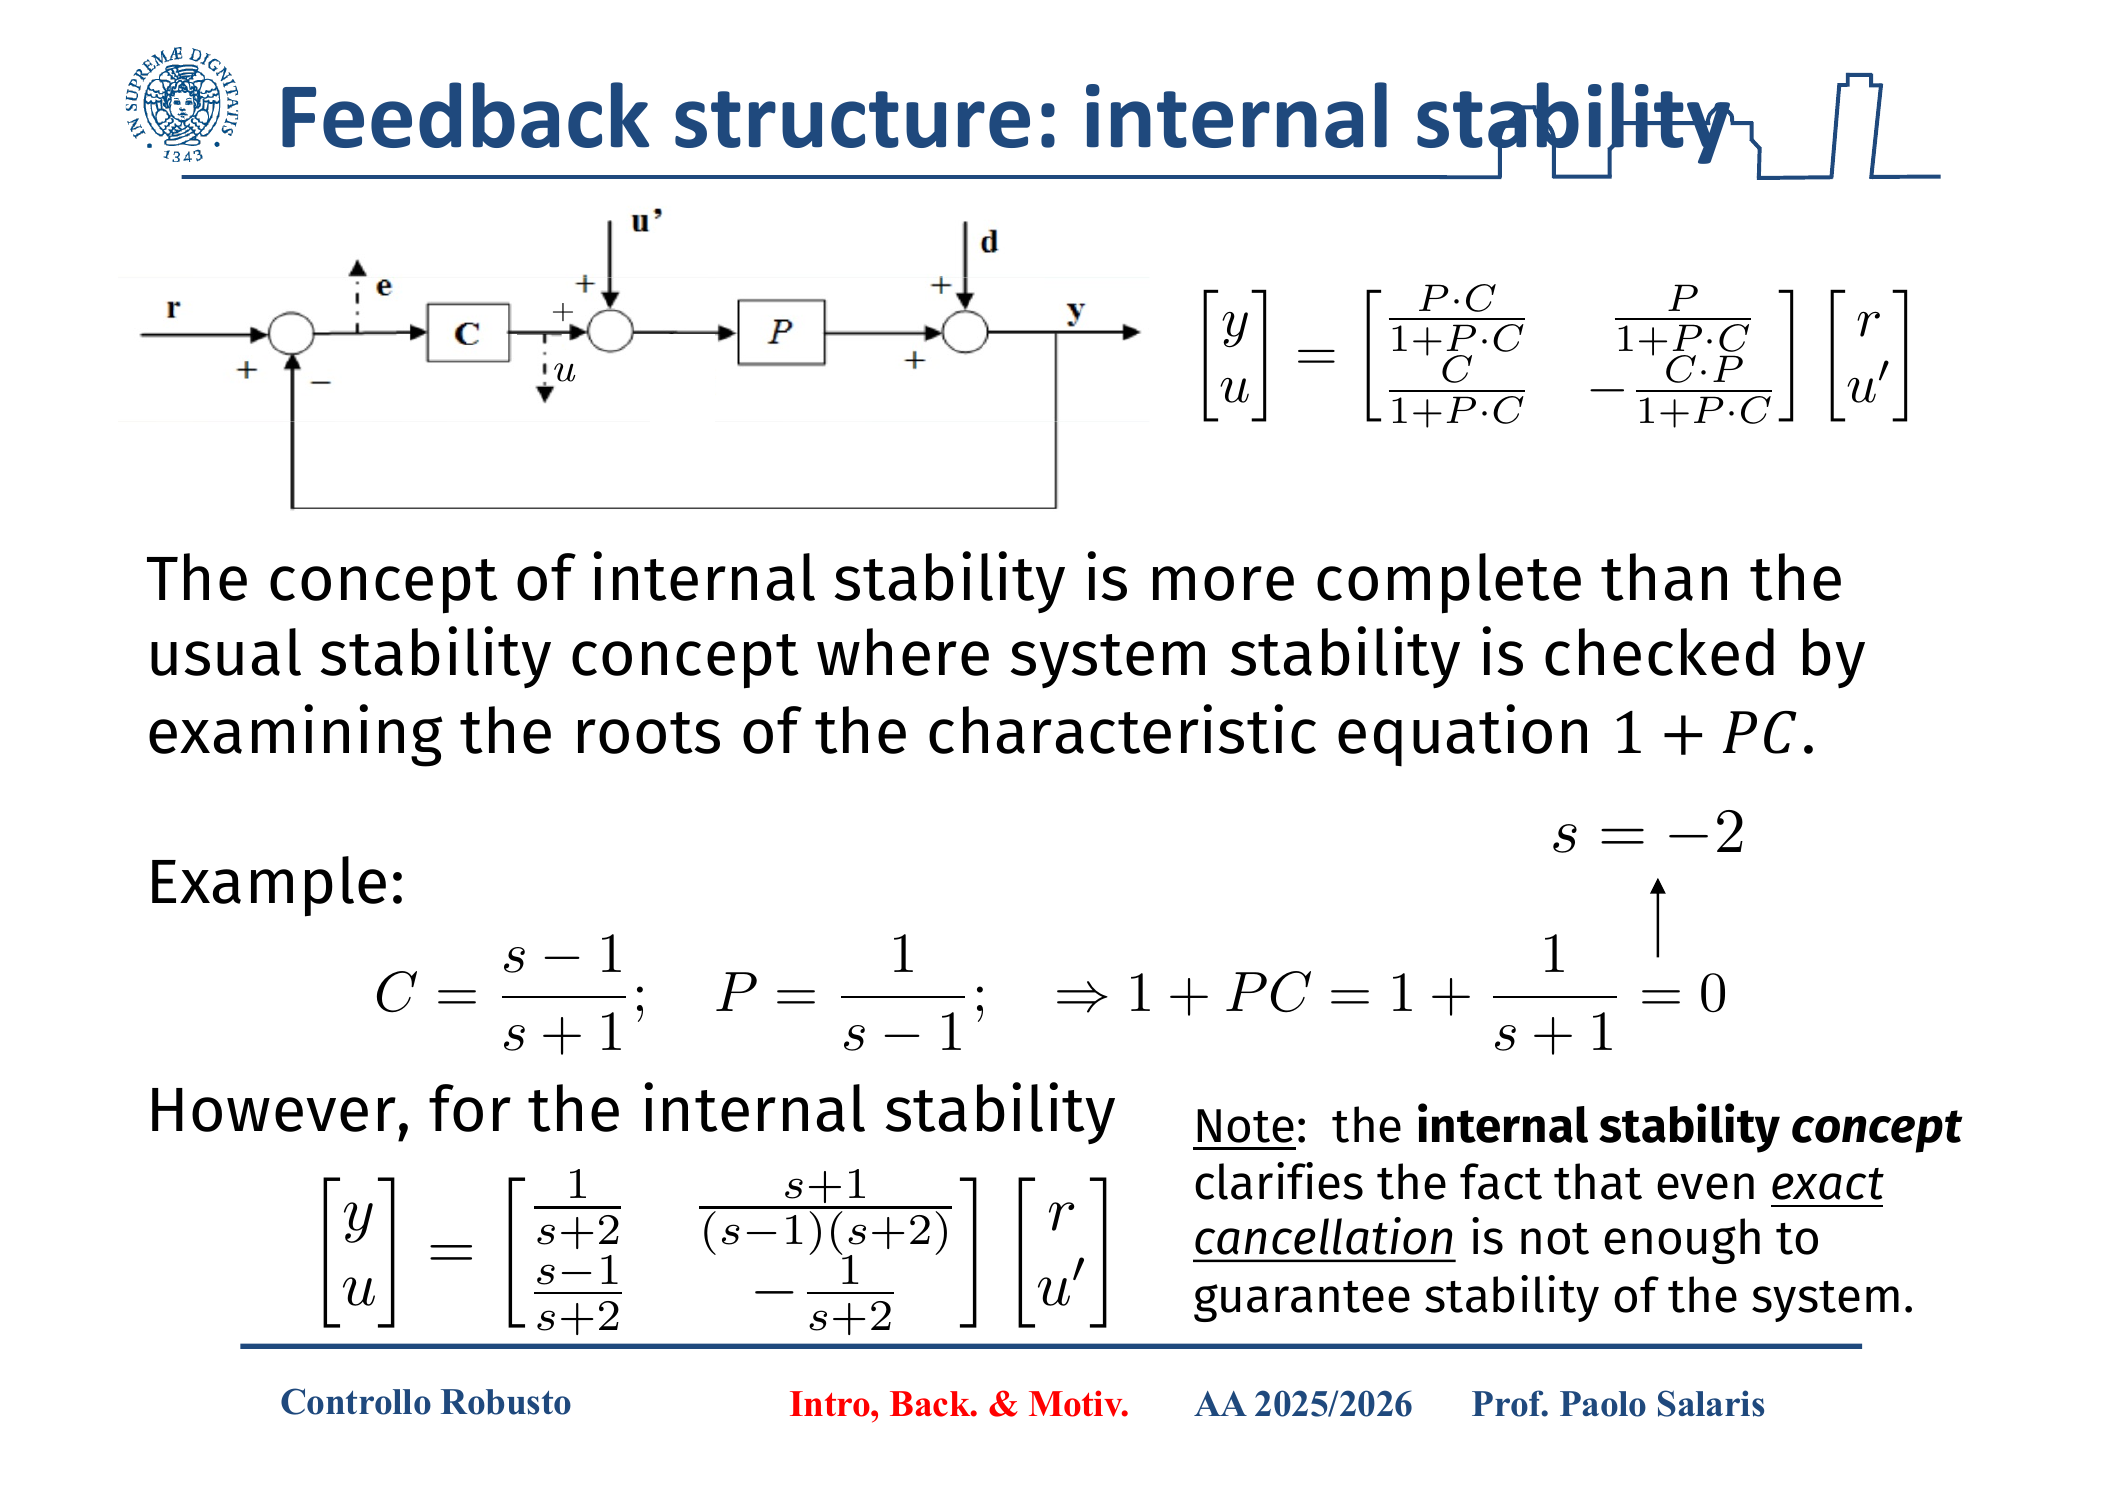
\includegraphics[width=0.78\textwidth]{images2/page-01.png}
\vfill
\begin{focusbox}
\textbf{Obiettivo del documento.} Questo elaborato riorganizza e approfondisce in italiano il contenuto del capitolo introduttivo dedicato a tre temi centrali del controllo robusto: la \emph{stabilità interna} delle interconnessioni in retroazione, le \emph{specifiche statiche e dinamiche} di progetto e il concetto di \emph{sensitività} rispetto alle incertezze parametriche. Le immagini originali delle slide sono state inserite nel testo per mantenere il legame con il materiale del corso.
\end{focusbox}
\vfill
{\large Basato sulle slide del corso AA 2025/2026\par}
\end{coverpage}

\section{Lezione 3}

\subsection{Visione d'insieme del capitolo}

Le slide di questo capitolo sviluppano un passaggio importante della teoria del controllo robusto. Dopo aver introdotto la retroazione, la well-posedness e i criteri di stabilità del sistema chiuso, il corso si sposta verso una domanda più precisa: \emph{quando una struttura di controllo non è solo stabile vista dall'esterno, ma è correttamente stabile in tutti i suoi segnali interni?} Da qui nasce il concetto di \emph{stabilità interna}.

Successivamente il materiale introduce due famiglie di obiettivi di progetto molto usate in automazione. Le prime sono le \emph{specifiche statiche}, cioè i requisiti di comportamento a regime, come annullamento dell'errore permanente o rigetto dei disturbi costanti. Le seconde sono le \emph{specifiche dinamiche}, cioè requisiti sul transitorio, come tempo di salita, tempo di assestamento e sovraelongazione. Infine il capitolo collega questi concetti alla \emph{sensitività}, cioè alla misura di quanto il comportamento del sistema cambi quando i parametri del modello si discostano dal valore nominale.

\begin{figure}[H]
    \centering
    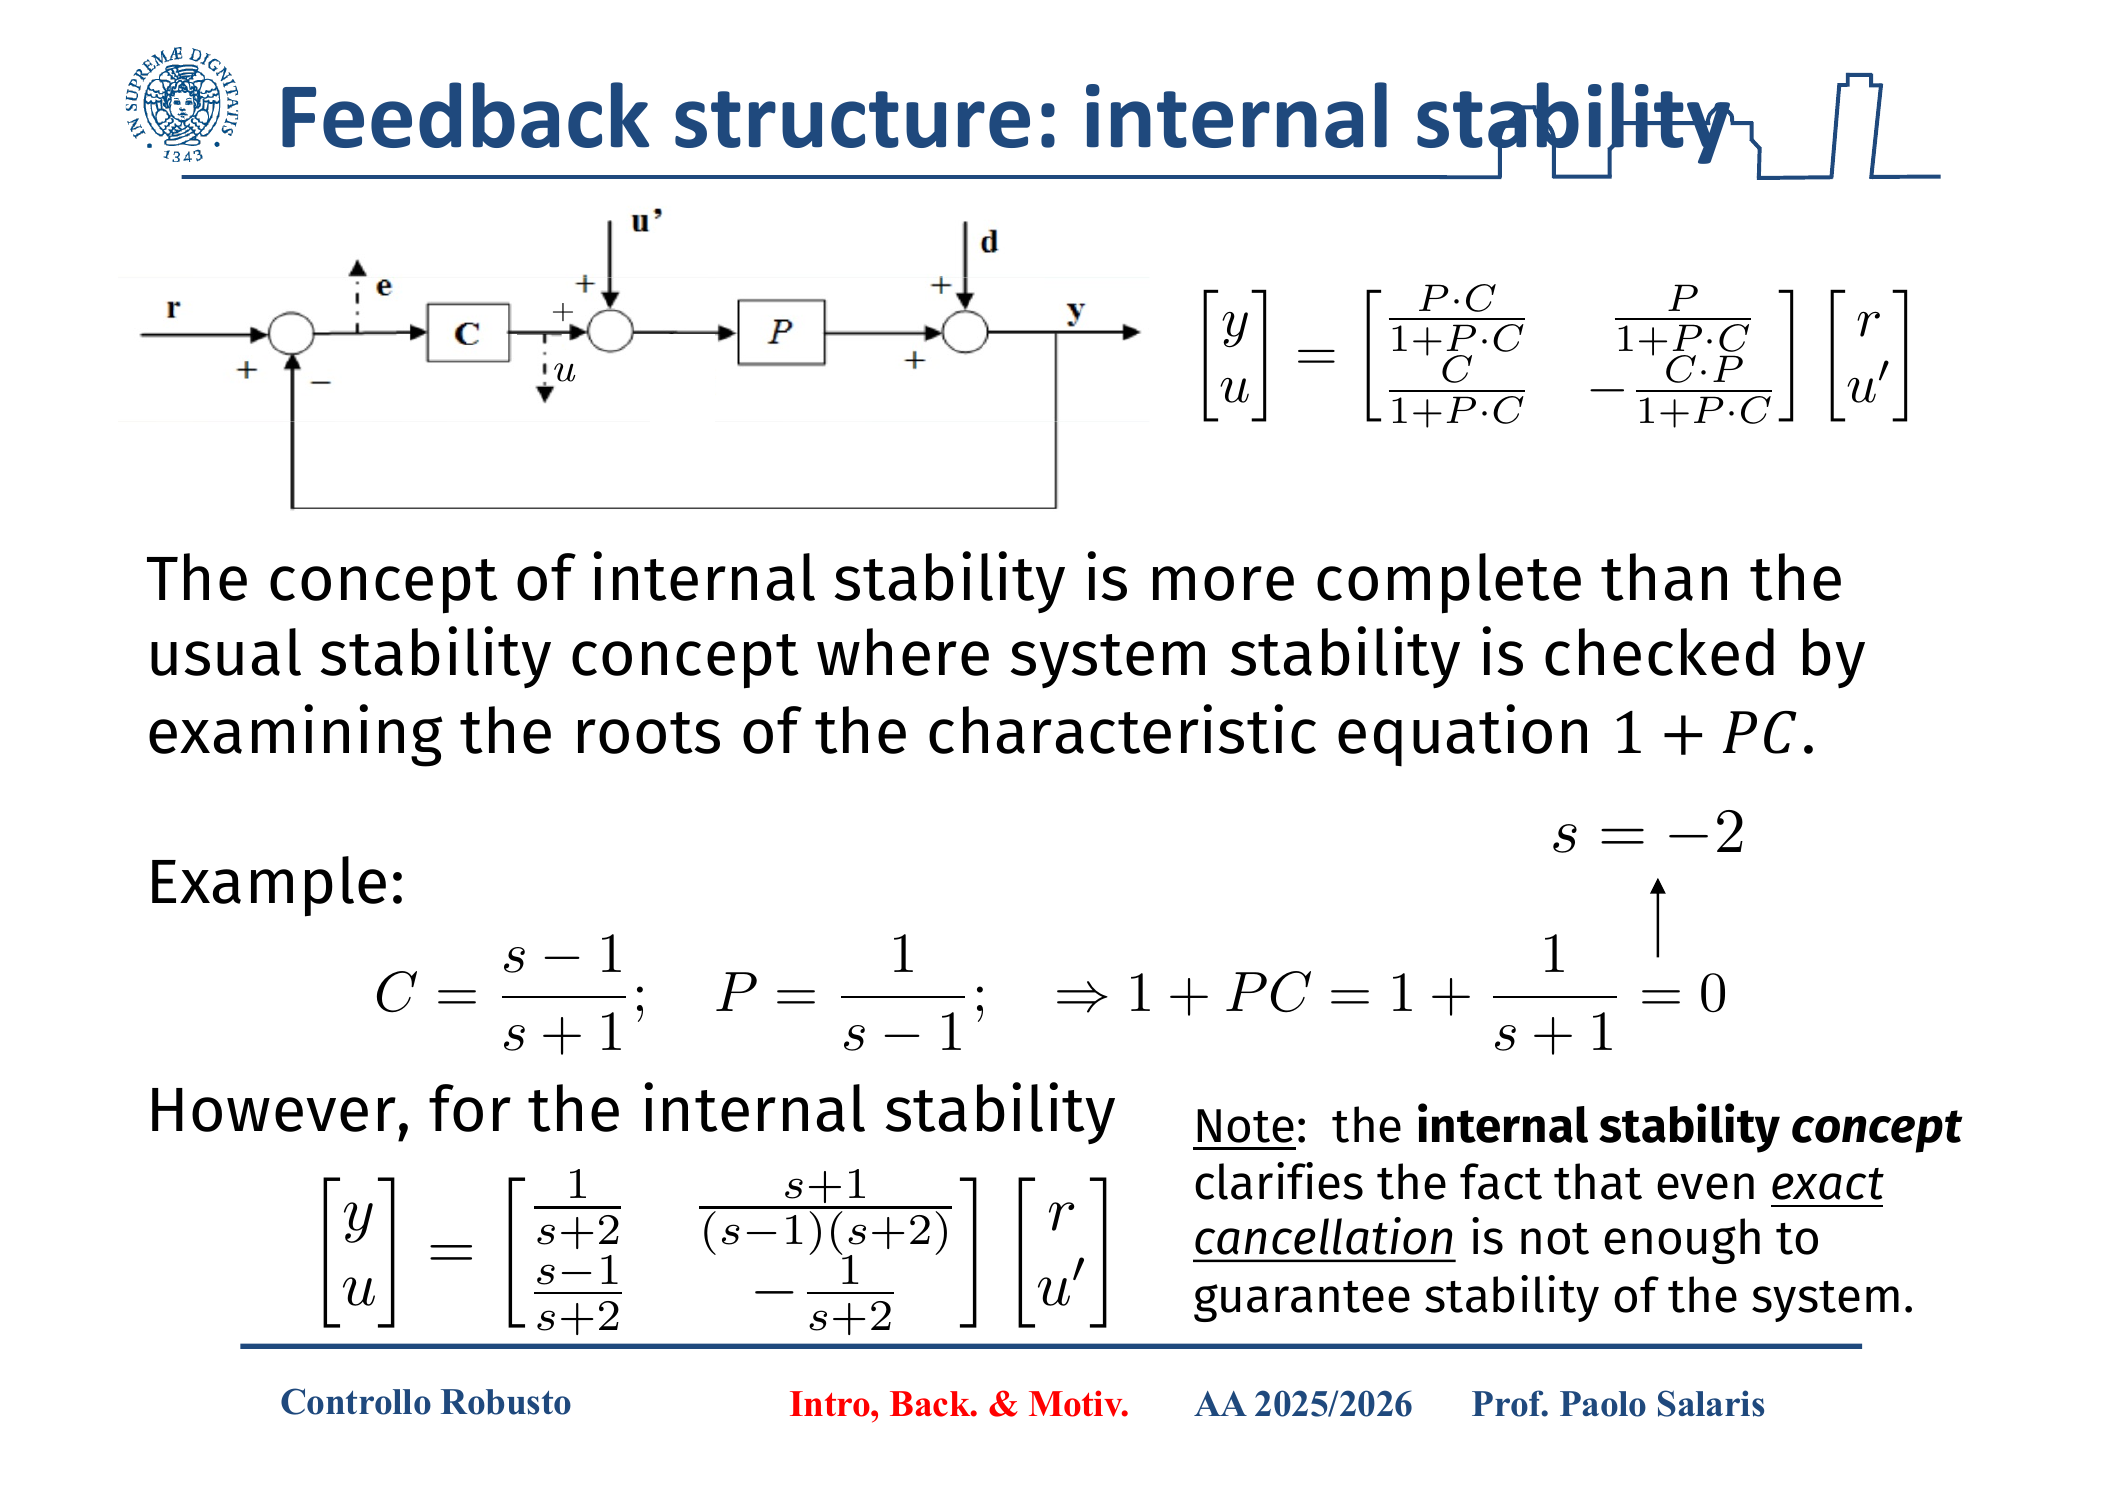
\includegraphics[width=0.78\textwidth]{images2/page-01.png}
    \caption{Prima slide del blocco: la stabilità interna viene introdotta come nozione più forte della sola stabilità dedotta da $1+PC=0$.}
\end{figure}

\begin{keybox}
La logica del capitolo è questa: non basta sapere che la funzione di trasferimento chiusa fra riferimento e uscita è stabile. In controllo robusto occorre garantire che \emph{tutte} le mappe tra segnali interni rilevanti siano stabili, e poi capire come questa proprietà si intrecci con prestazioni statiche, dinamiche e sensibilità alle incertezze.
\end{keybox}

\subsection{Stabilità interna della struttura di feedback}

\subsubsection{Perché la stabilità interna è più forte della stabilità usuale}

La prima slide parte da una struttura di retroazione standard e mostra una matrice di trasferimento che lega gli ingressi esterni ai segnali interni. Il messaggio è netto: il concetto di stabilità interna è \emph{più completo} della nozione usuale in cui si controllano solo le radici dell'equazione caratteristica $1+PC=0$.

Questo punto merita di essere esplicitato bene. Se si guarda solo alla funzione di trasferimento complessiva fra riferimento e uscita, si può concludere che il sistema è stabile perché il denominatore ridotto ha tutti i poli nel semipiano sinistro. Tuttavia, all'interno della struttura, alcune cancellazioni esatte tra poli e zeri possono nascondere dinamiche instabili che non compaiono più nella mappa esterna ma che continuano a vivere nei segnali interni o negli stati interni. In un modello puramente simbolico questa cancellazione può sembrare innocua; in un sistema fisico reale è invece pericolosa, perché basta una minima incertezza parametrica per far riemergere il polo instabile.

L'esempio mostrato in slide è istruttivo:
$$
C(s)=\frac{s-1}{s+1}, \qquad P(s)=\frac{1}{s-1}.
$$
Allora
$$
1+P(s)C(s)=1+\frac{1}{s+1}=0
\quad \Longrightarrow \quad s=-2.
$$
Guardando solo questa equazione sembrerebbe che il sistema chiuso sia stabile. Ma la matrice delle funzioni di trasferimento interne contiene termini come
$$
\frac{s+1}{(s-1)(s+2)}, \qquad \frac{s-1}{s+2},
$$
e quindi compare ancora il fattore instabile $(s-1)$ in alcune mappe interne. Questo basta per dire che il sistema non è internamente stabile.

\begin{figure}[H]
    \centering
    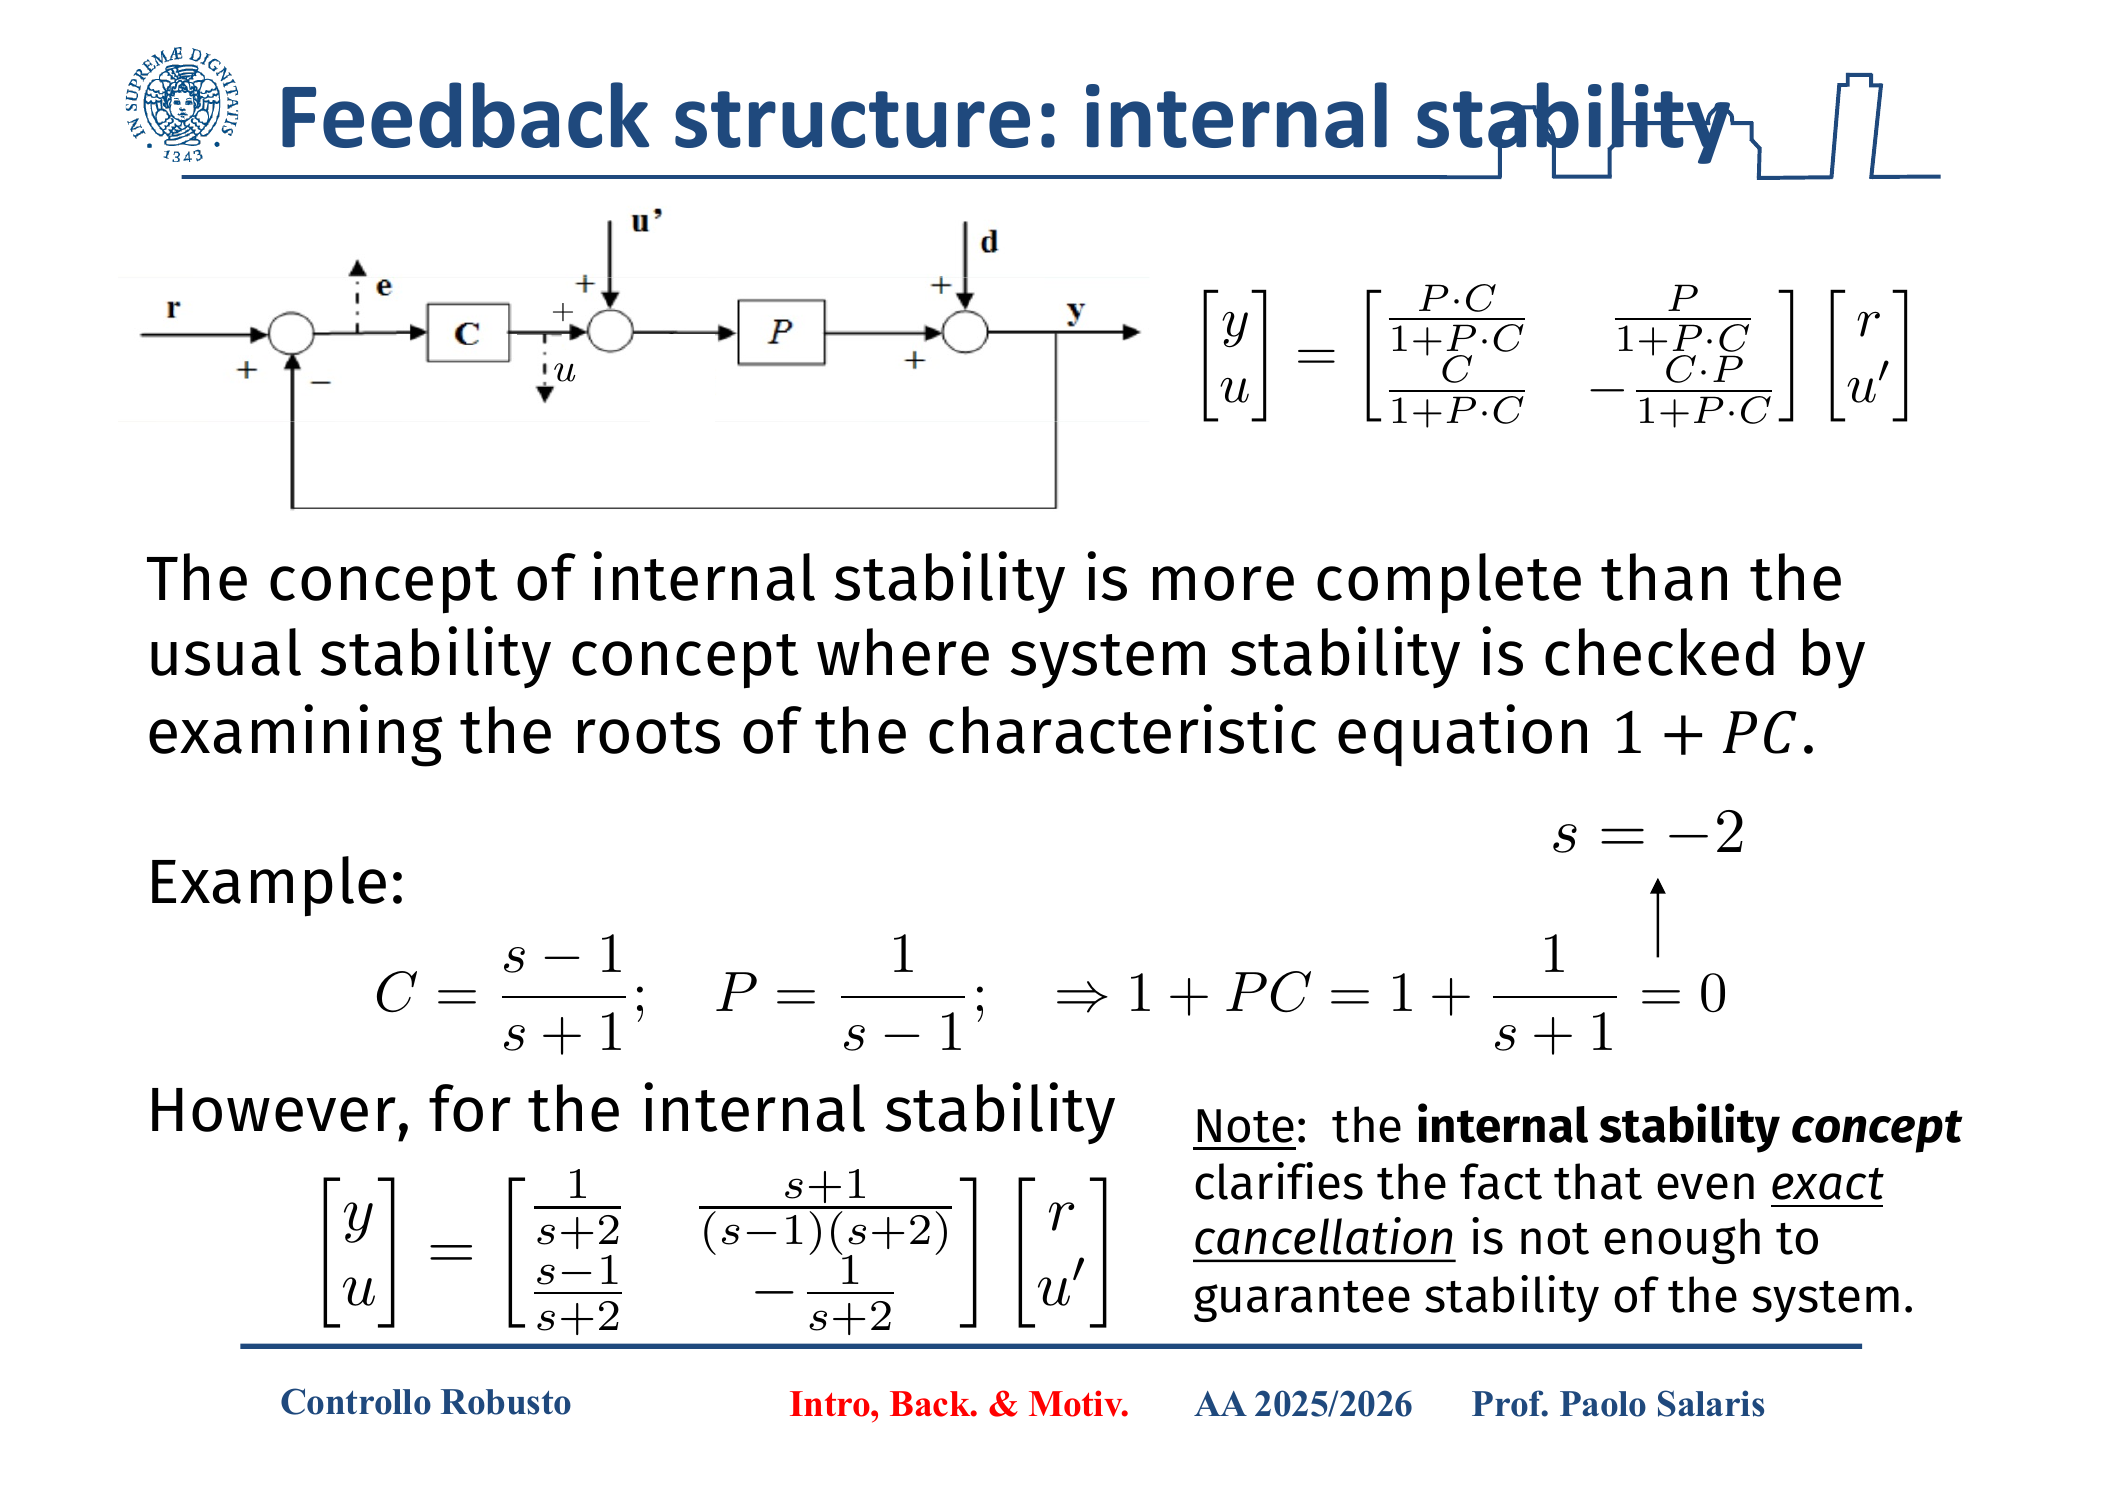
\includegraphics[width=0.8\textwidth]{images2/page-01.png}
    \caption{La slide evidenzia che una cancellazione esatta non garantisce la stabilità interna del sistema.}
\end{figure}

\subsubsection{Definizione in spazio di stato}

Le slide successive riformulano il problema in spazio di stato. Si assume che il feedback sia well-posed e che l'impianto $P(s)$ e il controllore $\hat K(s)$ siano stabilizzabili e rivelabili. Indicando con $x$ lo stato dell'impianto e con $\hat x$ lo stato del controllore, e ponendo nulli gli ingressi esterni $w_1$ e $w_2$, la struttura prende la forma
\begin{align*}
\dot x &= Ax + Be_1, & e_2 &= Cx + De_1, \\
\dot{\hat x} &= \hat A\hat x + \hat B e_2, & e_1 &= \hat C\hat x + \hat D e_2.
\end{align*}

La definizione che compare in slide può essere tradotta così: il sistema è \emph{internamente stabile} se l'origine $(x,\hat x)=(0,0)$ è asintoticamente stabile per ogni condizione iniziale quando gli ingressi esterni sono nulli. Questa è una definizione forte, perché non osserva solo un'uscita particolare ma tutta la dinamica combinata dell'interconnessione.

\begin{figure}[H]
    \centering
    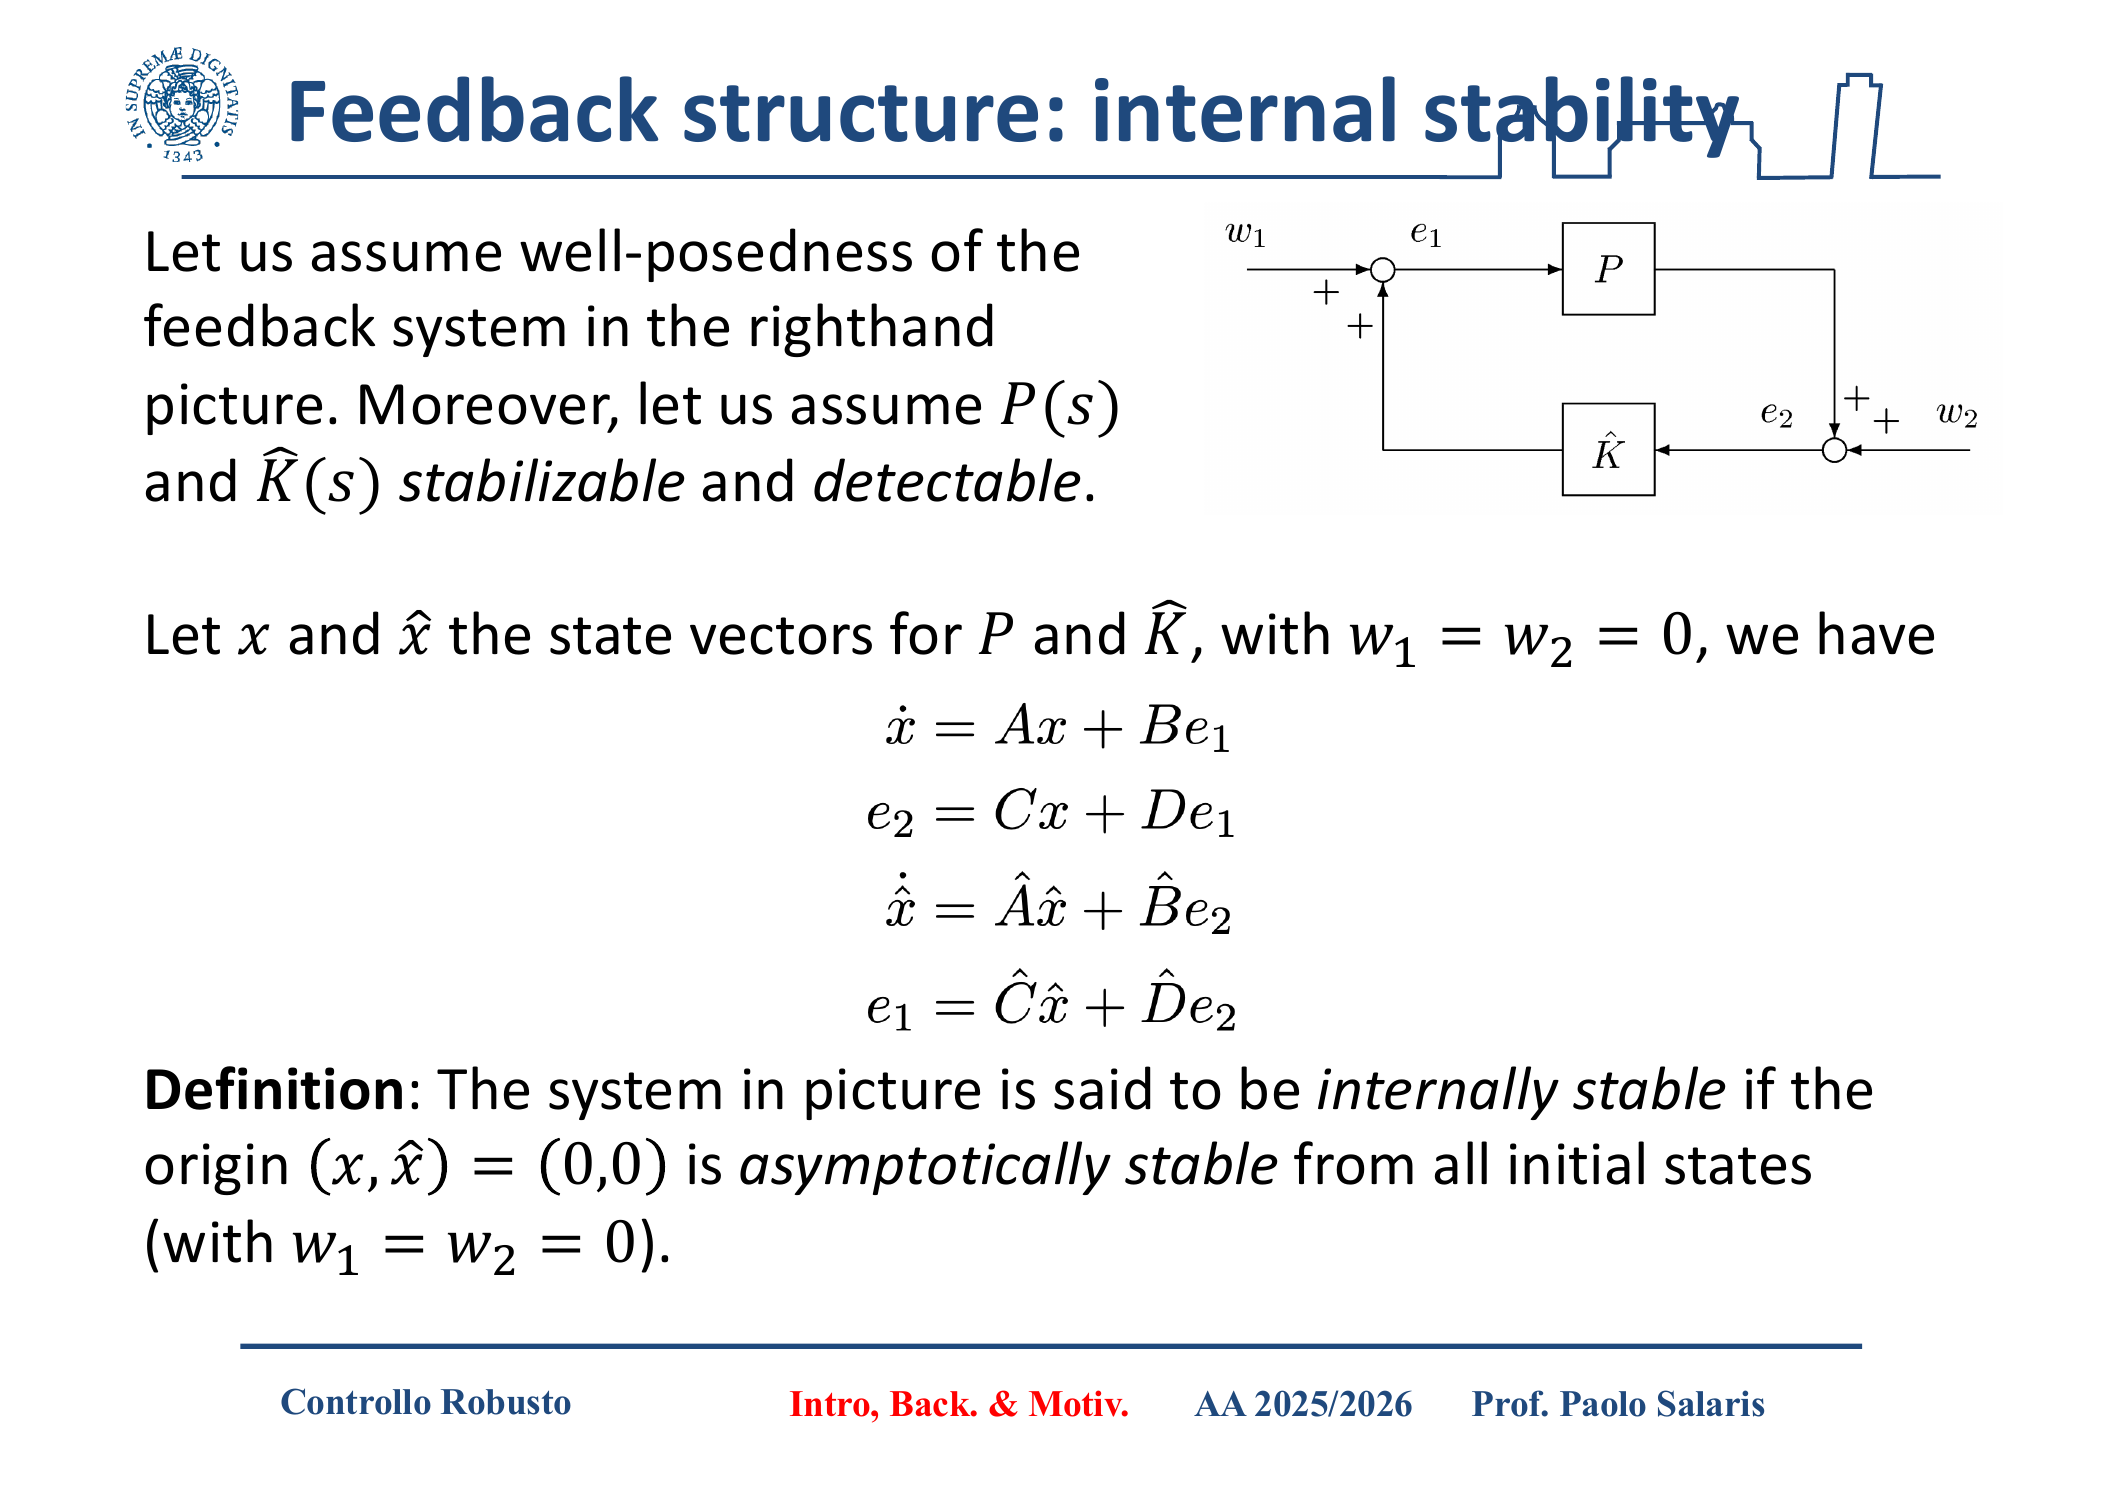
\includegraphics[width=0.78\textwidth]{images2/page-02.png}
    \caption{Definizione di stabilità interna tramite la dinamica congiunta di impianto e controllore.}
\end{figure}

\subsubsection{Caratterizzazione tramite matrice dinamica chiusa}

Per ottenere una condizione concreta, si risolvono le equazioni algebriche che definiscono $e_1$ ed $e_2$. Le slide mostrano che, in assenza di ingressi esterni,
$$
\begin{bmatrix} e_1 \\ e_2 \end{bmatrix}
=
\begin{bmatrix} I & -\hat D \\ -D & I \end{bmatrix}^{-1}
\begin{bmatrix} 0 & \hat C \\ C & 0 \end{bmatrix}
\begin{bmatrix} x \\ \hat x \end{bmatrix}.
$$
Sostituendo questa relazione nelle equazioni dinamiche di impianto e controllore si ottiene un sistema autonomo della forma
$$
\frac{d}{dt}
\begin{bmatrix} x \\ \hat x \end{bmatrix}
=
\tilde A
\begin{bmatrix} x \\ \hat x \end{bmatrix},
$$
con
$$
\tilde A =
\begin{bmatrix} A & 0 \\ 0 & \hat A \end{bmatrix}
+
\begin{bmatrix} B & 0 \\ 0 & \hat B \end{bmatrix}
\begin{bmatrix} I & -\hat D \\ -D & I \end{bmatrix}^{-1}
\begin{bmatrix} 0 & \hat C \\ C & 0 \end{bmatrix}.
$$

Il lemma riportato nelle slide è allora naturale: il sistema è internamente stabile se e solo se la matrice $\tilde A$ è di Hurwitz. In altre parole, la stabilità interna coincide con la stabilità asintotica della dinamica combinata del sistema interconnesso.

\begin{figure}[H]
    \centering
    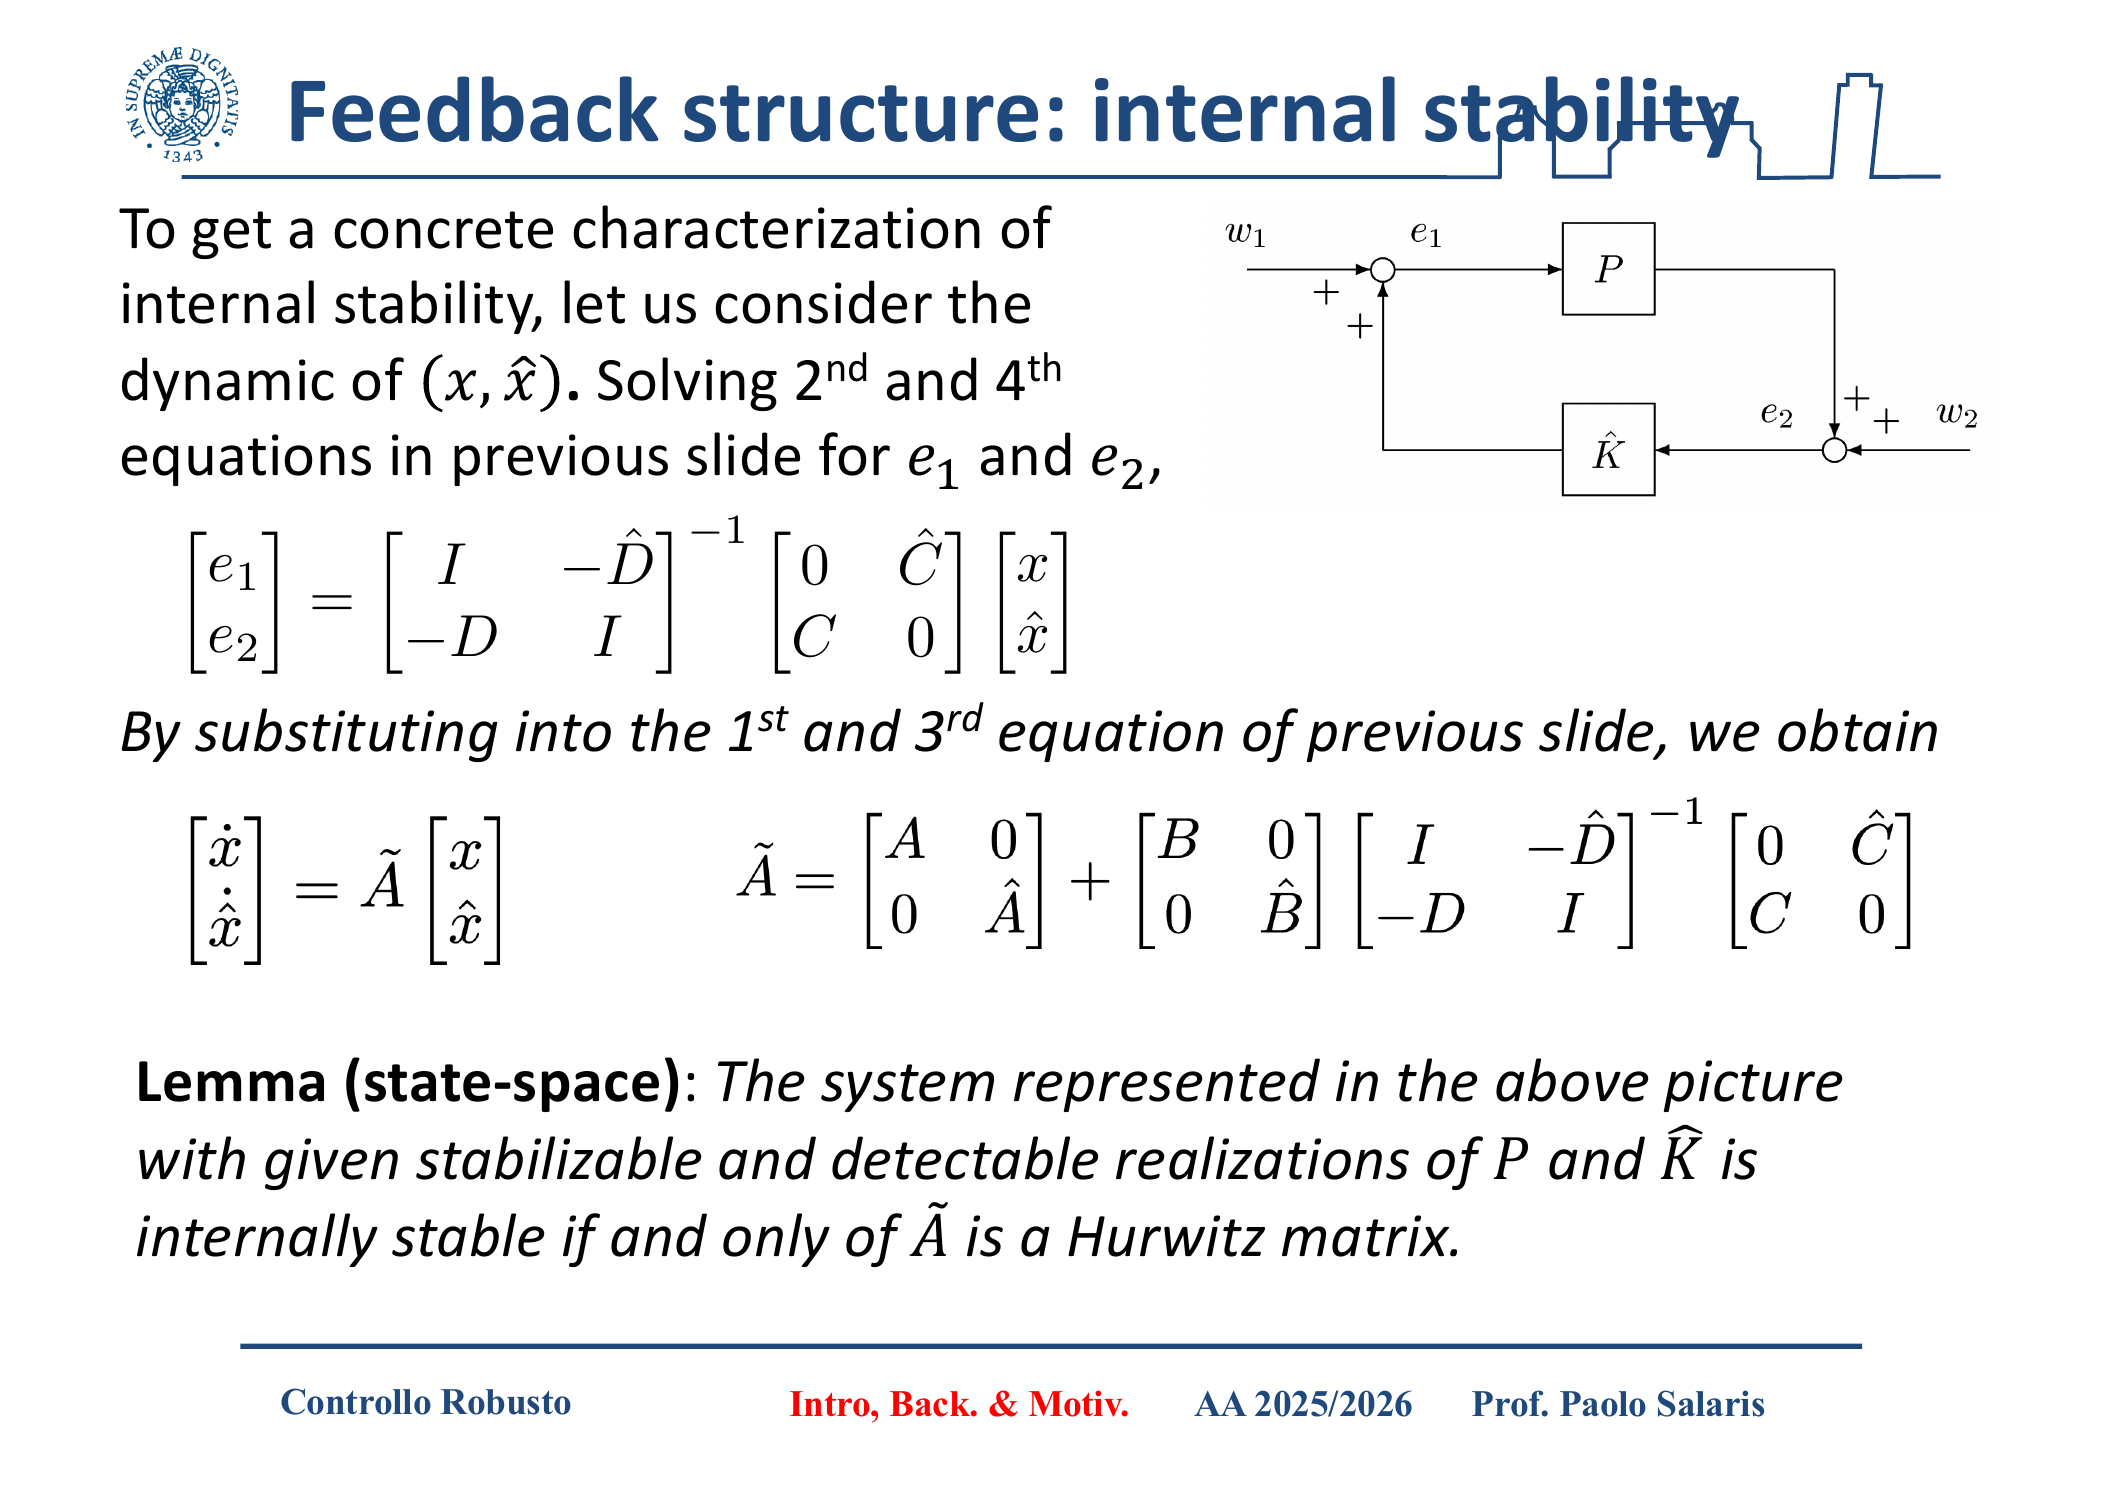
\includegraphics[width=0.78\textwidth]{images2/page-03.png}
    \caption{Caratterizzazione in spazio di stato: la stabilità interna equivale al fatto che la matrice chiusa $\tilde A$ sia di Hurwitz.}
\end{figure}

\subsubsection{Caratterizzazione tramite matrici di trasferimento}

Le slide mostrano anche la formulazione equivalente in termini di matrici di trasferimento. Per la struttura indicata si ha
$$
\begin{bmatrix} I & -\hat K \\ -P & I \end{bmatrix}
\begin{bmatrix} e_1 \\ e_2 \end{bmatrix}
=
\begin{bmatrix} w_1 \\ w_2 \end{bmatrix},
$$
quindi
$$
\begin{bmatrix} e_1 \\ e_2 \end{bmatrix}
=
\begin{bmatrix} I & -\hat K \\ -P & I \end{bmatrix}^{-1}
\begin{bmatrix} w_1 \\ w_2 \end{bmatrix}.
$$
La stabilità interna equivale al fatto che tutte le voci della matrice che mappa $(w_1,w_2)$ in $(e_1,e_2)$ siano funzioni di trasferimento proprie, razionali reali e stabili. Le slide sviluppano esplicitamente tale inversa come
$$
\begin{bmatrix}
(I-\hat K P)^{-1} & \hat K(I-P\hat K)^{-1} \\
P(I-\hat K P)^{-1} & (I-P\hat K)^{-1}
\end{bmatrix}.
$$

Questa scrittura è molto importante, perché rende visibile un fatto spesso usato in robustezza: non basta che una singola funzione, per esempio la funzione di sensibilità complementare, sia stabile. Devono esserlo \emph{tutti} i blocchi che collegano le perturbazioni ai segnali interni.

\begin{figure}[H]
    \centering
    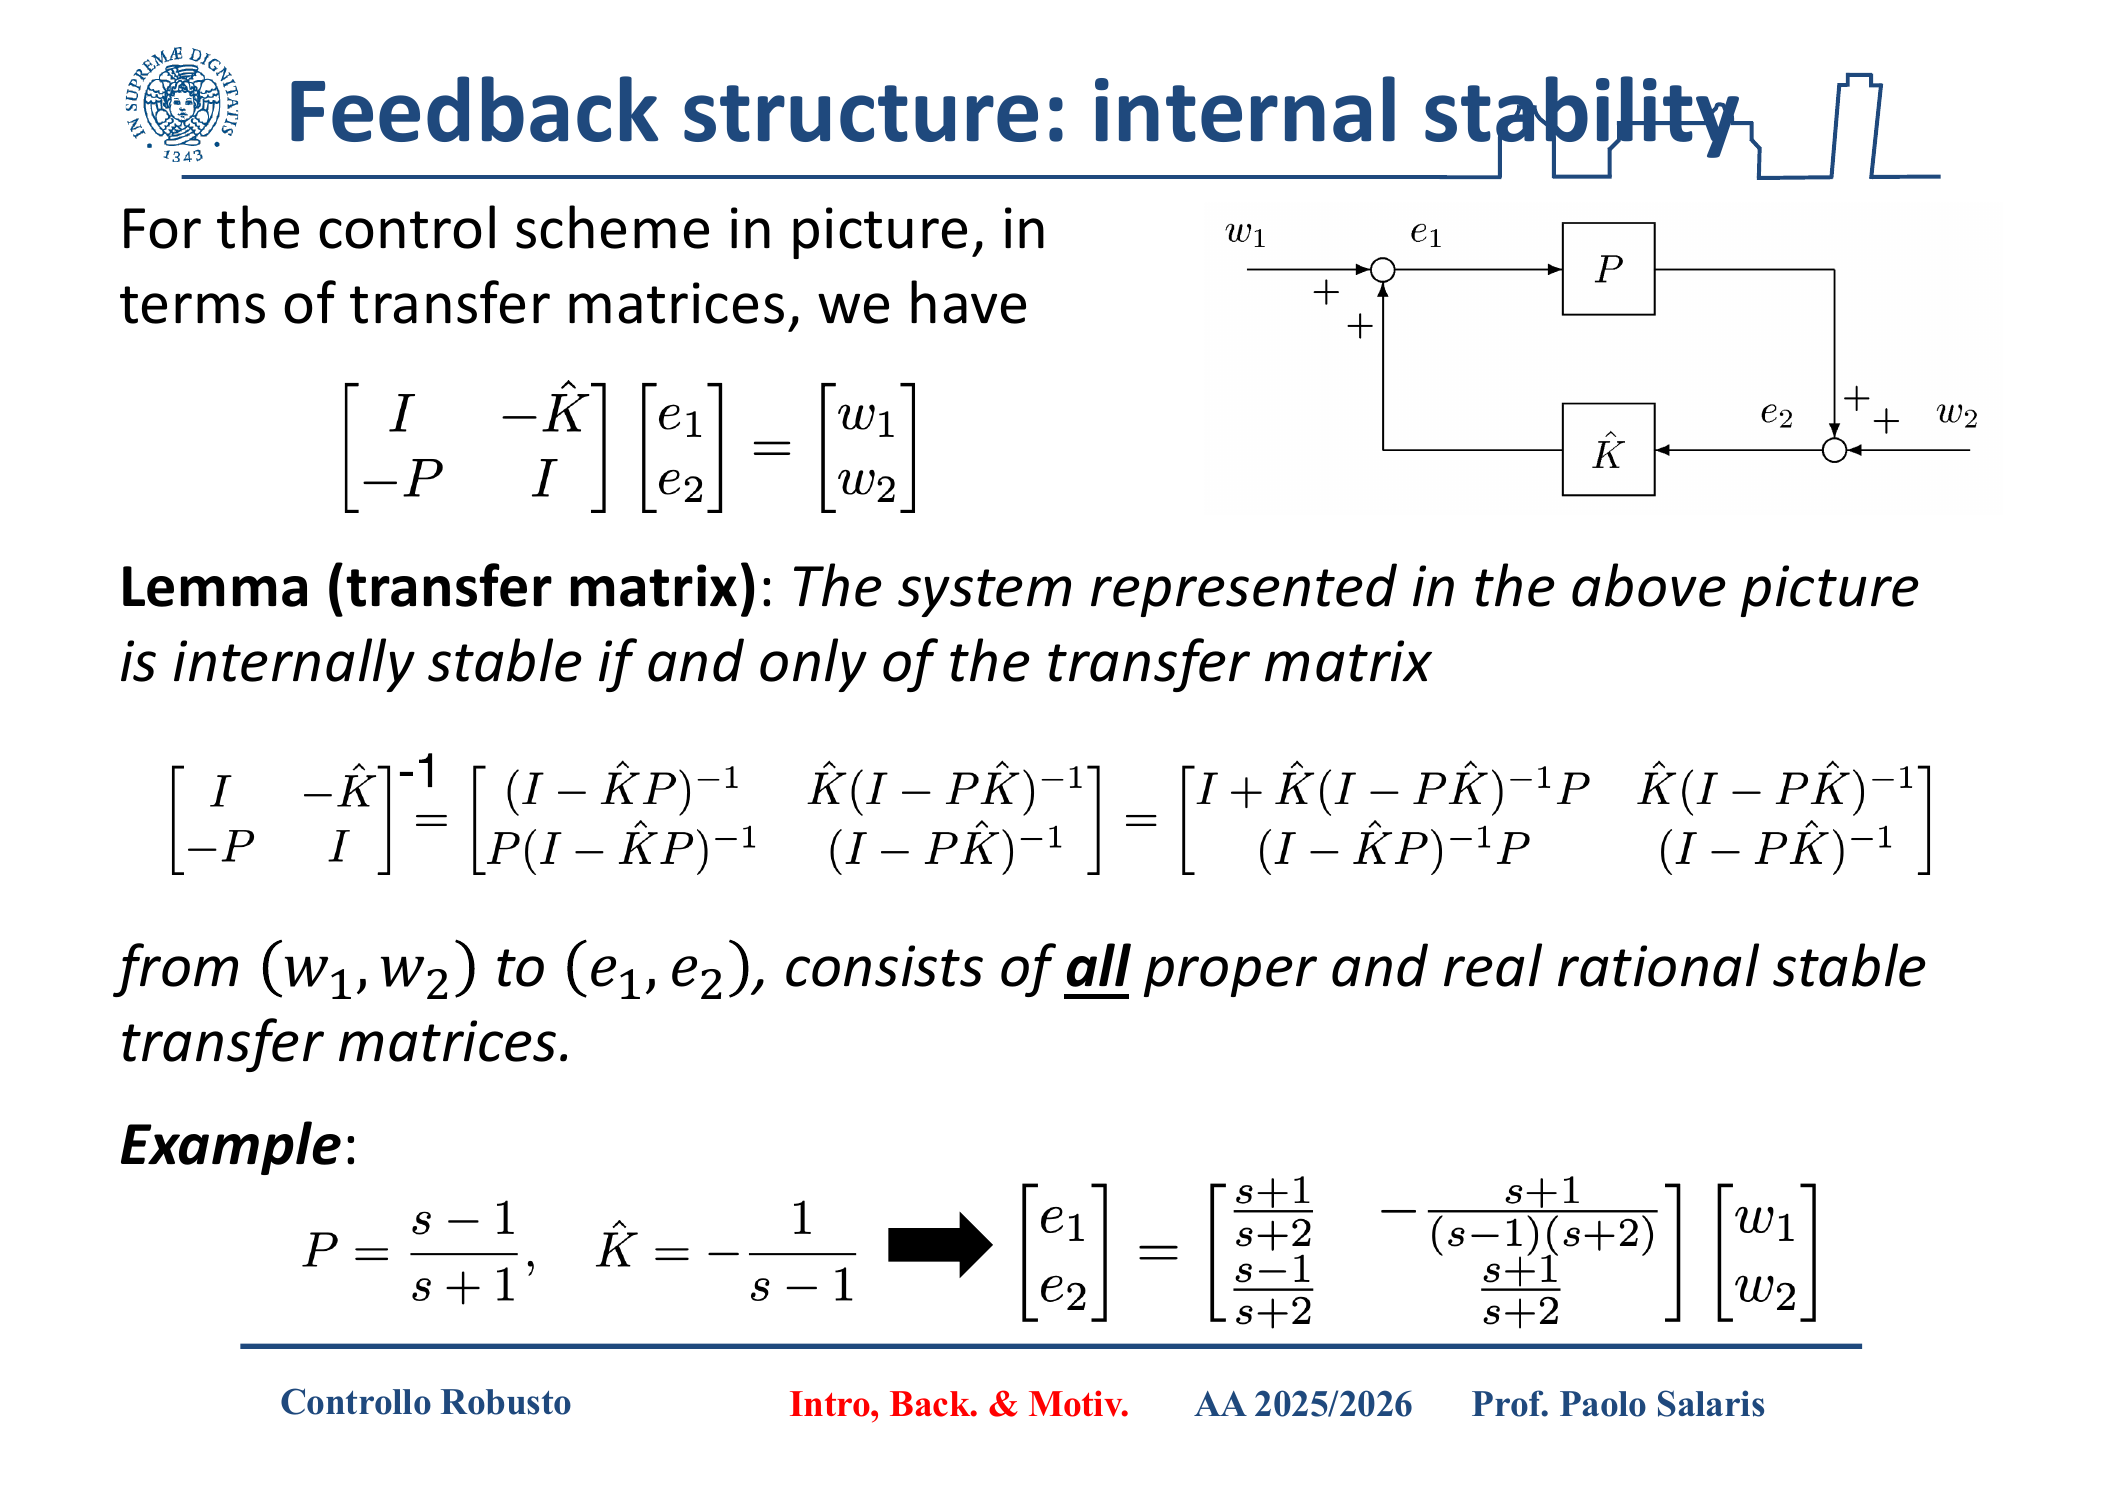
\includegraphics[width=0.78\textwidth]{images2/page-04.png}
    \caption{Forma matriciale della mappa fra ingressi esterni e segnali interni.}
\end{figure}

\subsubsection{Corollari pratici}

Le slide estraggono poi tre corollari molto usati nella pratica.

Se $\hat K$ è stabile, allora il sistema è internamente stabile se e solo se è well-posed e la funzione
$$
P(I-\hat K P)^{-1}
$$
è propria e stabile.

Se sia $P$ sia $\hat K$ sono stabili, allora la condizione si semplifica ulteriormente: il sistema è internamente stabile se e solo se è well-posed e
$$
(I-P\hat K)^{-1}
$$
è stabile. Questo è il caso tipico in cui la stabilità interna coincide con la stabilità della ``resolvente'' del loop.

Infine la slide riporta un teorema che coinvolge il numero di poli instabili di $P$ e $\hat K$. Il messaggio è che la sola assenza di zeri di $\det(I-P\hat K)$ nel semipiano destro non basta in generale. Occorre anche che il numero di poli instabili di $P\hat K$ sia quello atteso e che l'inversa di $I-P\hat K$ sia effettivamente stabile.

\begin{figure}[H]
    \centering
    \begin{subfigure}{0.49\textwidth}
        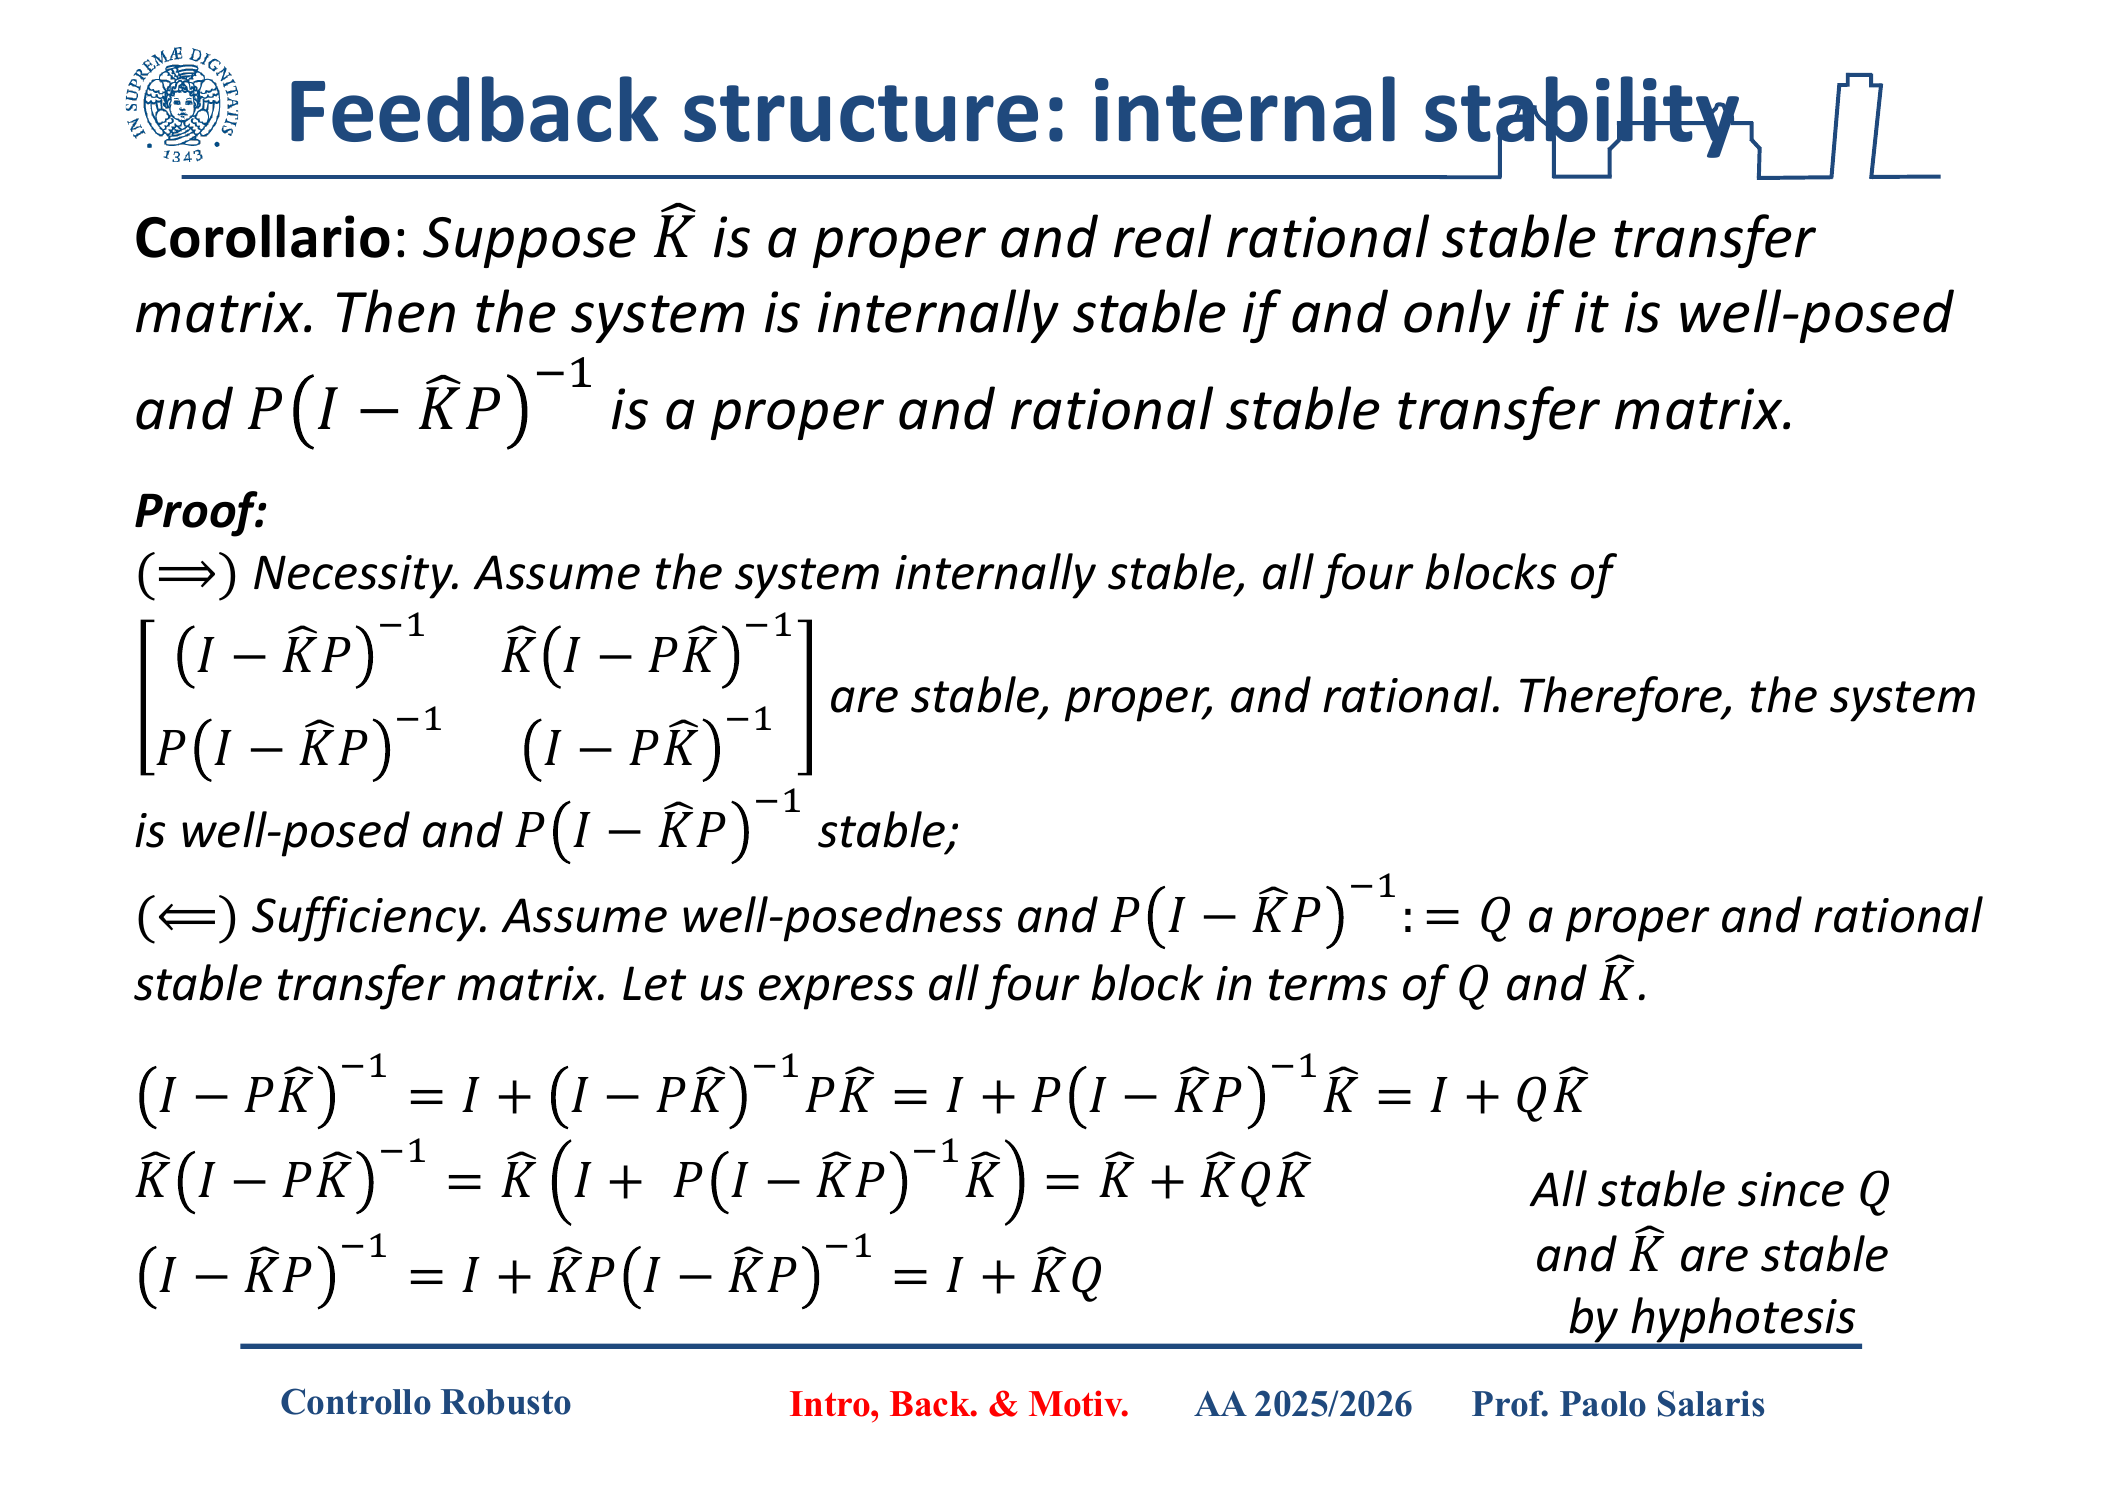
\includegraphics[width=\linewidth]{images2/page-05.png}
        \caption{Primo corollario.}
    \end{subfigure}
    \hfill
    \begin{subfigure}{0.49\textwidth}
        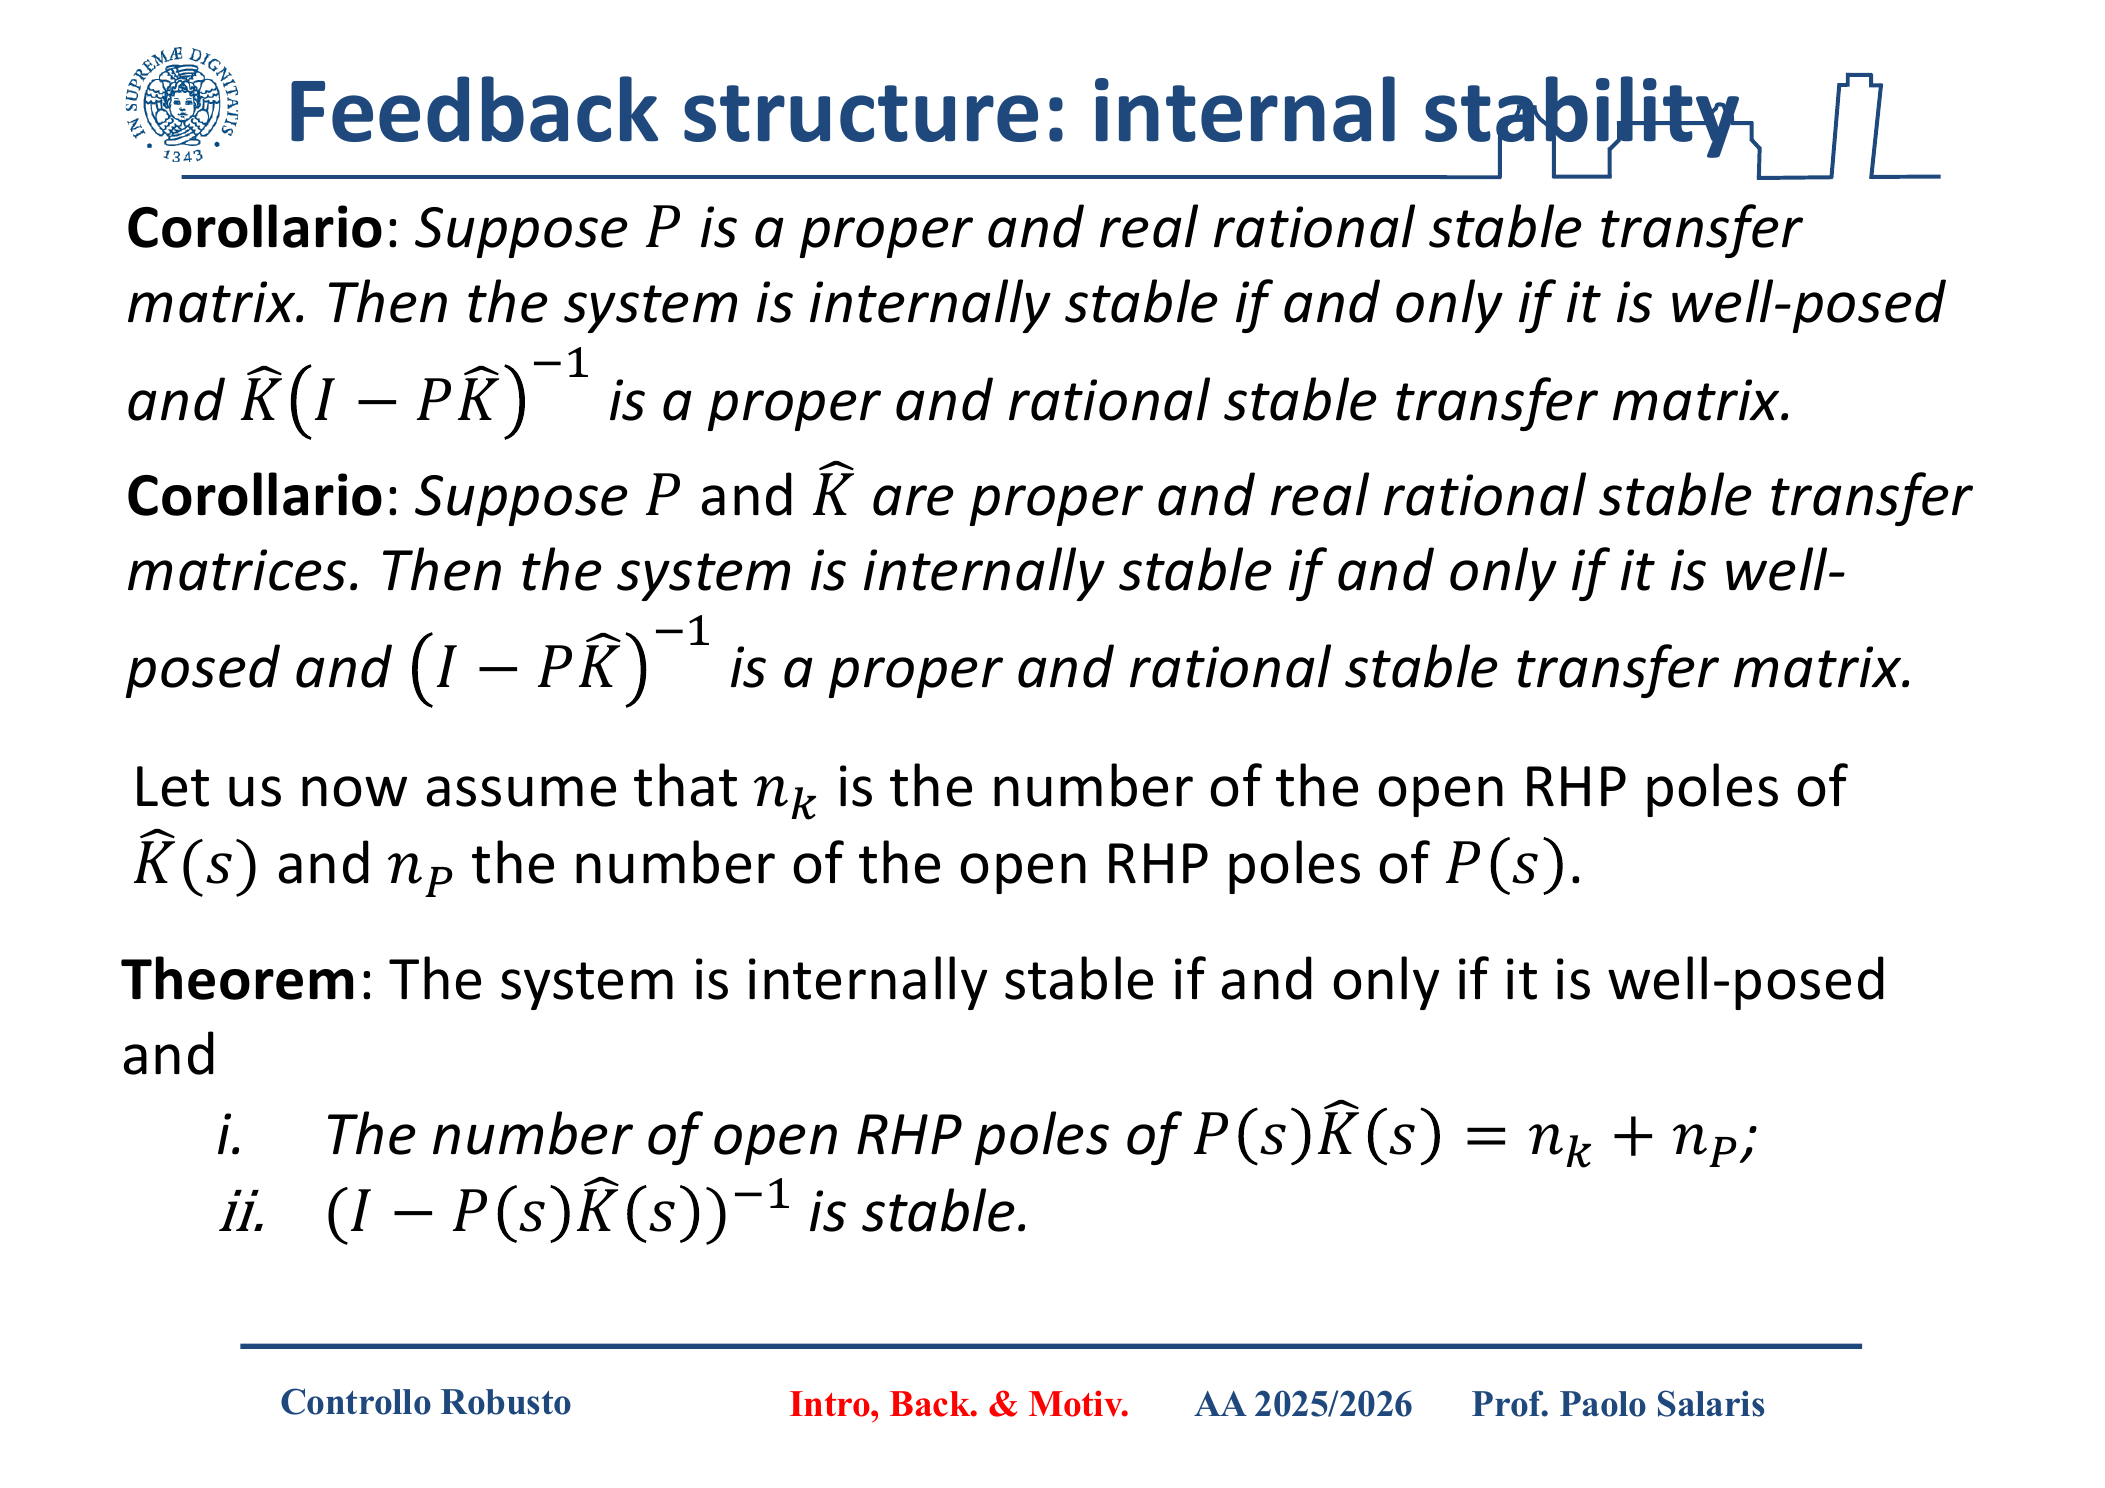
\includegraphics[width=\linewidth]{images2/page-06.png}
        \caption{Secondo corollario e teorema sui poli instabili.}
    \end{subfigure}
    \caption{Condizioni equivalenti di stabilità interna in casi particolarmente utili.}
\end{figure}

\subsubsection{Esempio matriciale: perché il determinante non basta}

L'esempio della slide 7 è molto istruttivo. Si scelgono due matrici di trasferimento $2\times2$ tali che
$$
\det(I-P\hat K)=\frac{(s+2)^2}{(s+1)^2},
$$
quindi il determinante non ha zeri nel semipiano destro. Potrebbe sembrare una situazione rassicurante. Ma la slide mostra che
$$
(I-P\hat K)^{-1}
$$
contiene il termine
$$
-\frac{(s+1)^2}{(s+2)^2(s-1)},
$$
che ha un polo instabile in $s=1$. Dunque l'inversa non è stabile e il sistema chiuso non è internamente stabile.

La lezione da portare a casa è netta: in sistemi MIMO o, più in generale, in strutture di interconnessione complesse, la condizione su un determinante può essere solo necessaria ma non sufficiente. La robustezza richiede controllo puntuale delle mappe interne.

\begin{figure}[H]
    \centering
    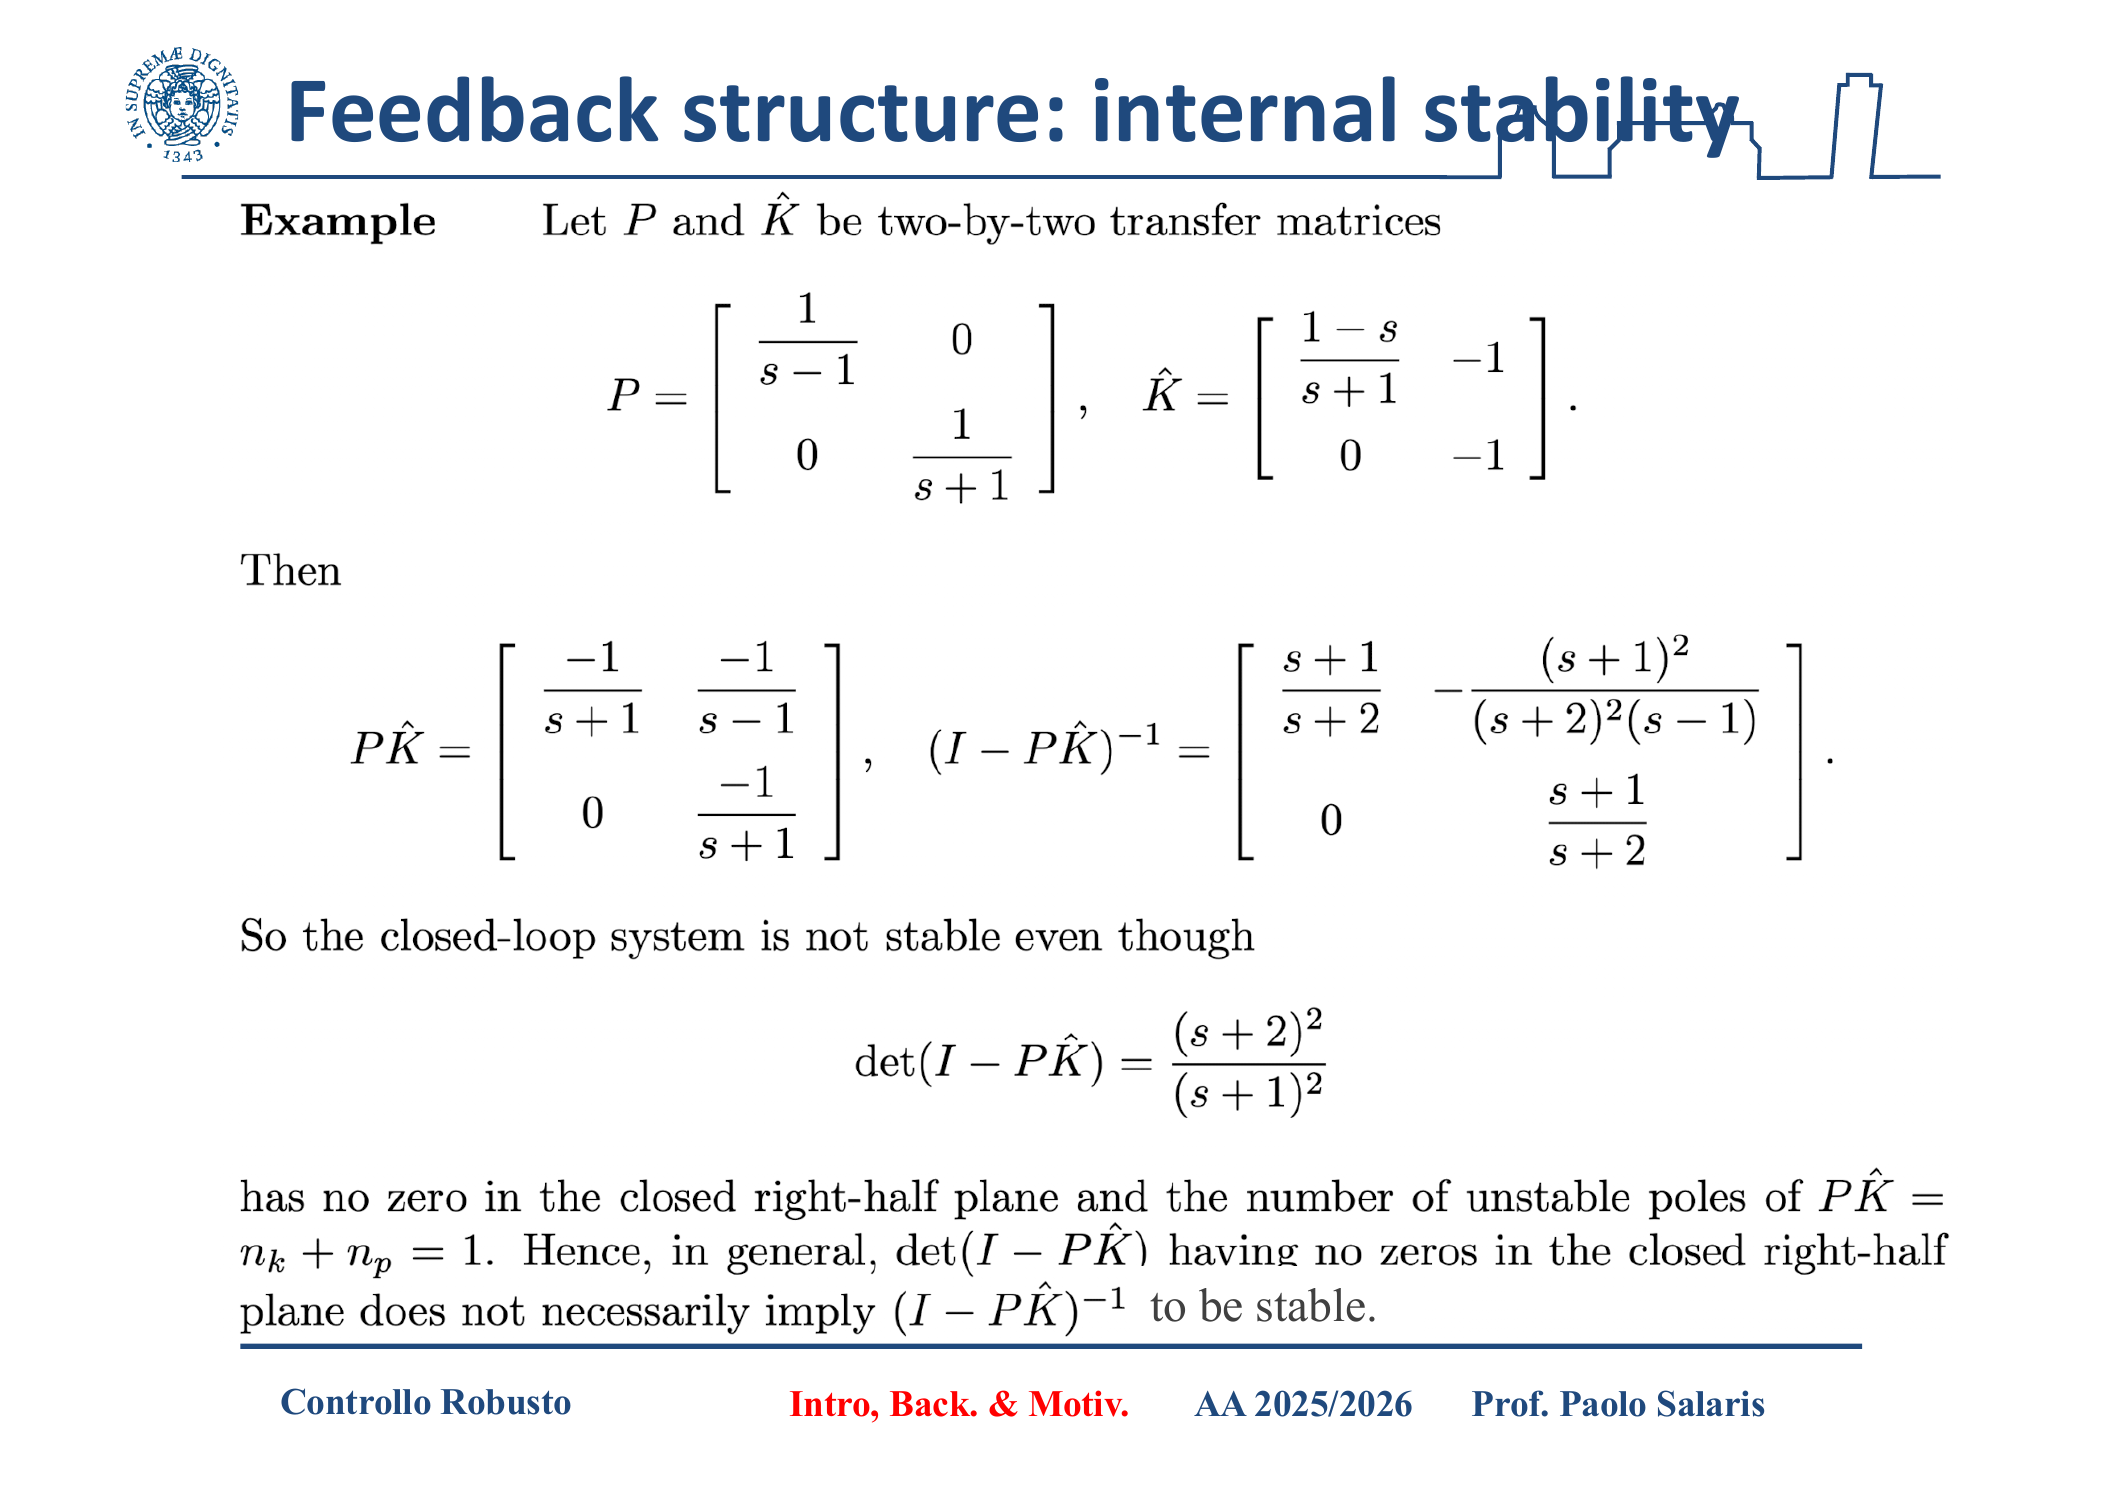
\includegraphics[width=0.78\textwidth]{images2/page-07.png}
    \caption{Esempio MIMO in cui $\det(I-P\hat K)$ non basta a garantire la stabilità interna.}
\end{figure}

\subsection{Specifiche statiche e dinamiche}

\subsubsection{Tre famiglie di specifiche di progetto}

La slide 8 introduce la tripartizione classica delle specifiche di progetto:
\begin{enumerate}
    \item specifiche statiche;
    \item specifiche dinamiche;
    \item specifiche di robustezza.
\end{enumerate}
In questo blocco il focus è sui primi due gruppi. Le specifiche statiche riguardano il comportamento a regime. Le specifiche dinamiche riguardano il transitorio.

\begin{figure}[H]
    \centering
    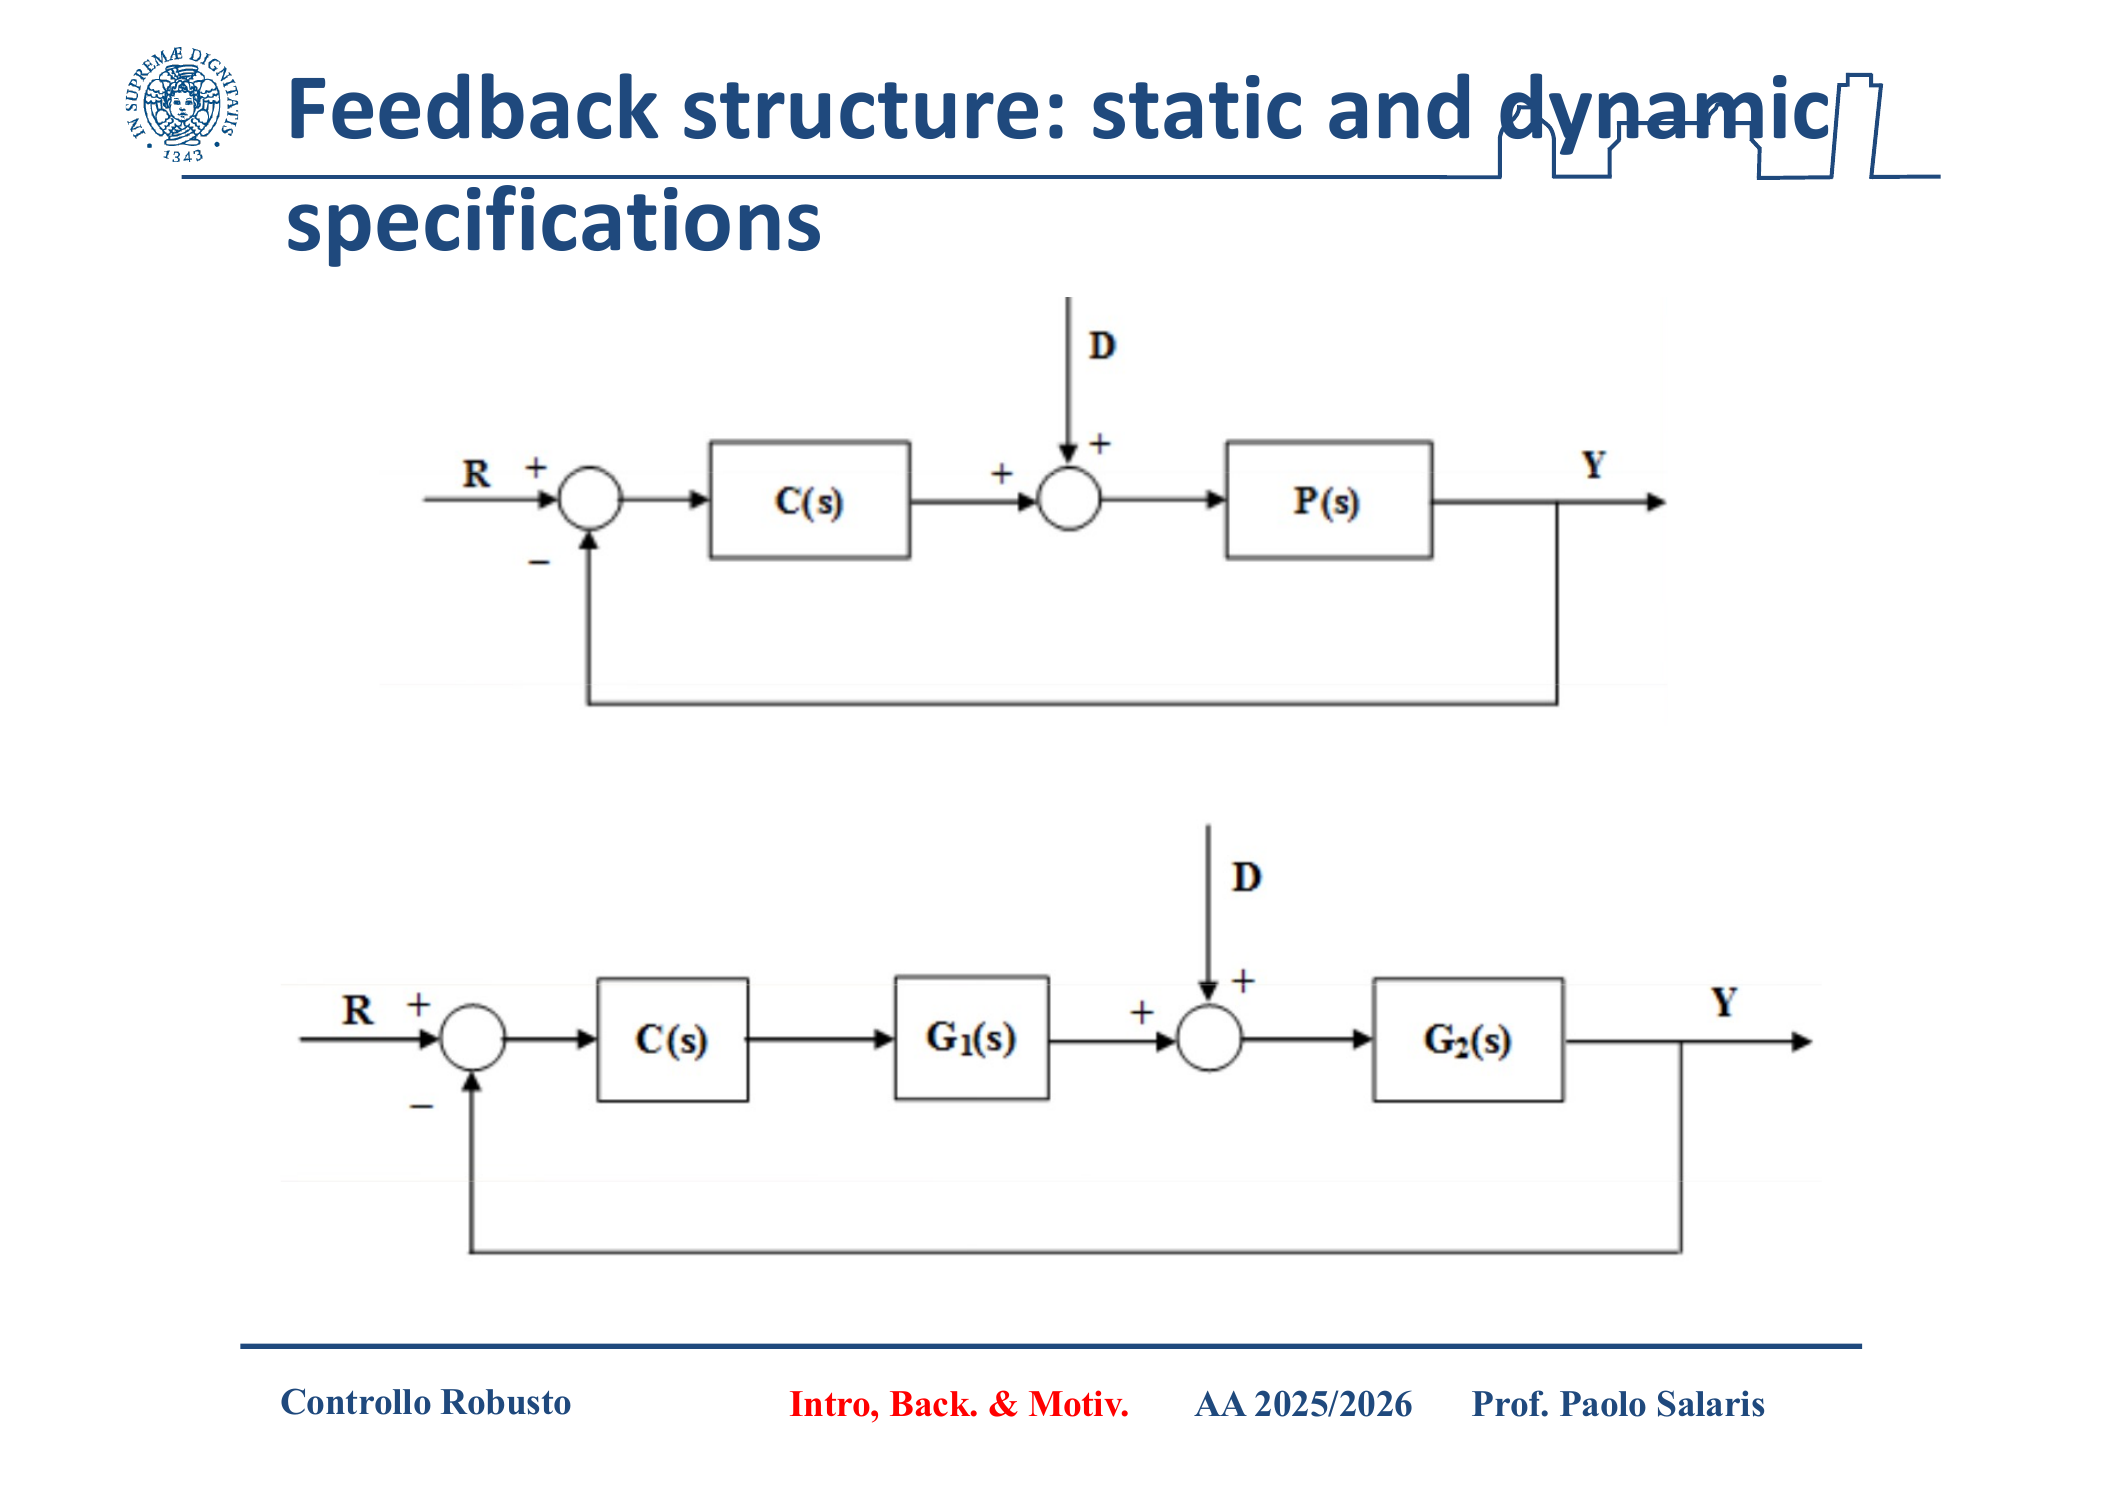
\includegraphics[width=0.7\textwidth]{images2/page-09.png}
    \caption{Schema di feedback usato per discutere riferimento, disturbo e uscita.}
\end{figure}

\subsubsection{Risposta a riferimento e a disturbo}

Nella struttura a due blocchi di processo $G_1(s)$ e $G_2(s)$ con controllore $C(s)$, l'uscita può essere scritta come
$$
Y(s)=G_c(s)R(s)+G_d(s)D(s),
$$
con
$$
G_c(s)=\frac{C(s)G_1(s)G_2(s)}{1+C(s)G_1(s)G_2(s)},
\qquad
G_d(s)=\frac{G_2(s)}{1+C(s)G_1(s)G_2(s)}.
$$

Queste due funzioni hanno un significato preciso. $G_c(s)$ è la mappa chiusa dal riferimento all'uscita. $G_d(s)$ è la mappa dal disturbo additivo all'uscita. Se il sistema è stabile, il teorema del valore finale permette di identificare il comportamento a regime guardando i valori a bassa frequenza, cioè in $s=0$.

I valori ideali sono
$$
G_c(0)=1, \qquad G_d(0)=0.
$$
Il primo significa inseguimento perfetto del riferimento costante. Il secondo significa rigetto perfetto del disturbo costante.

\begin{figure}[H]
    \centering
    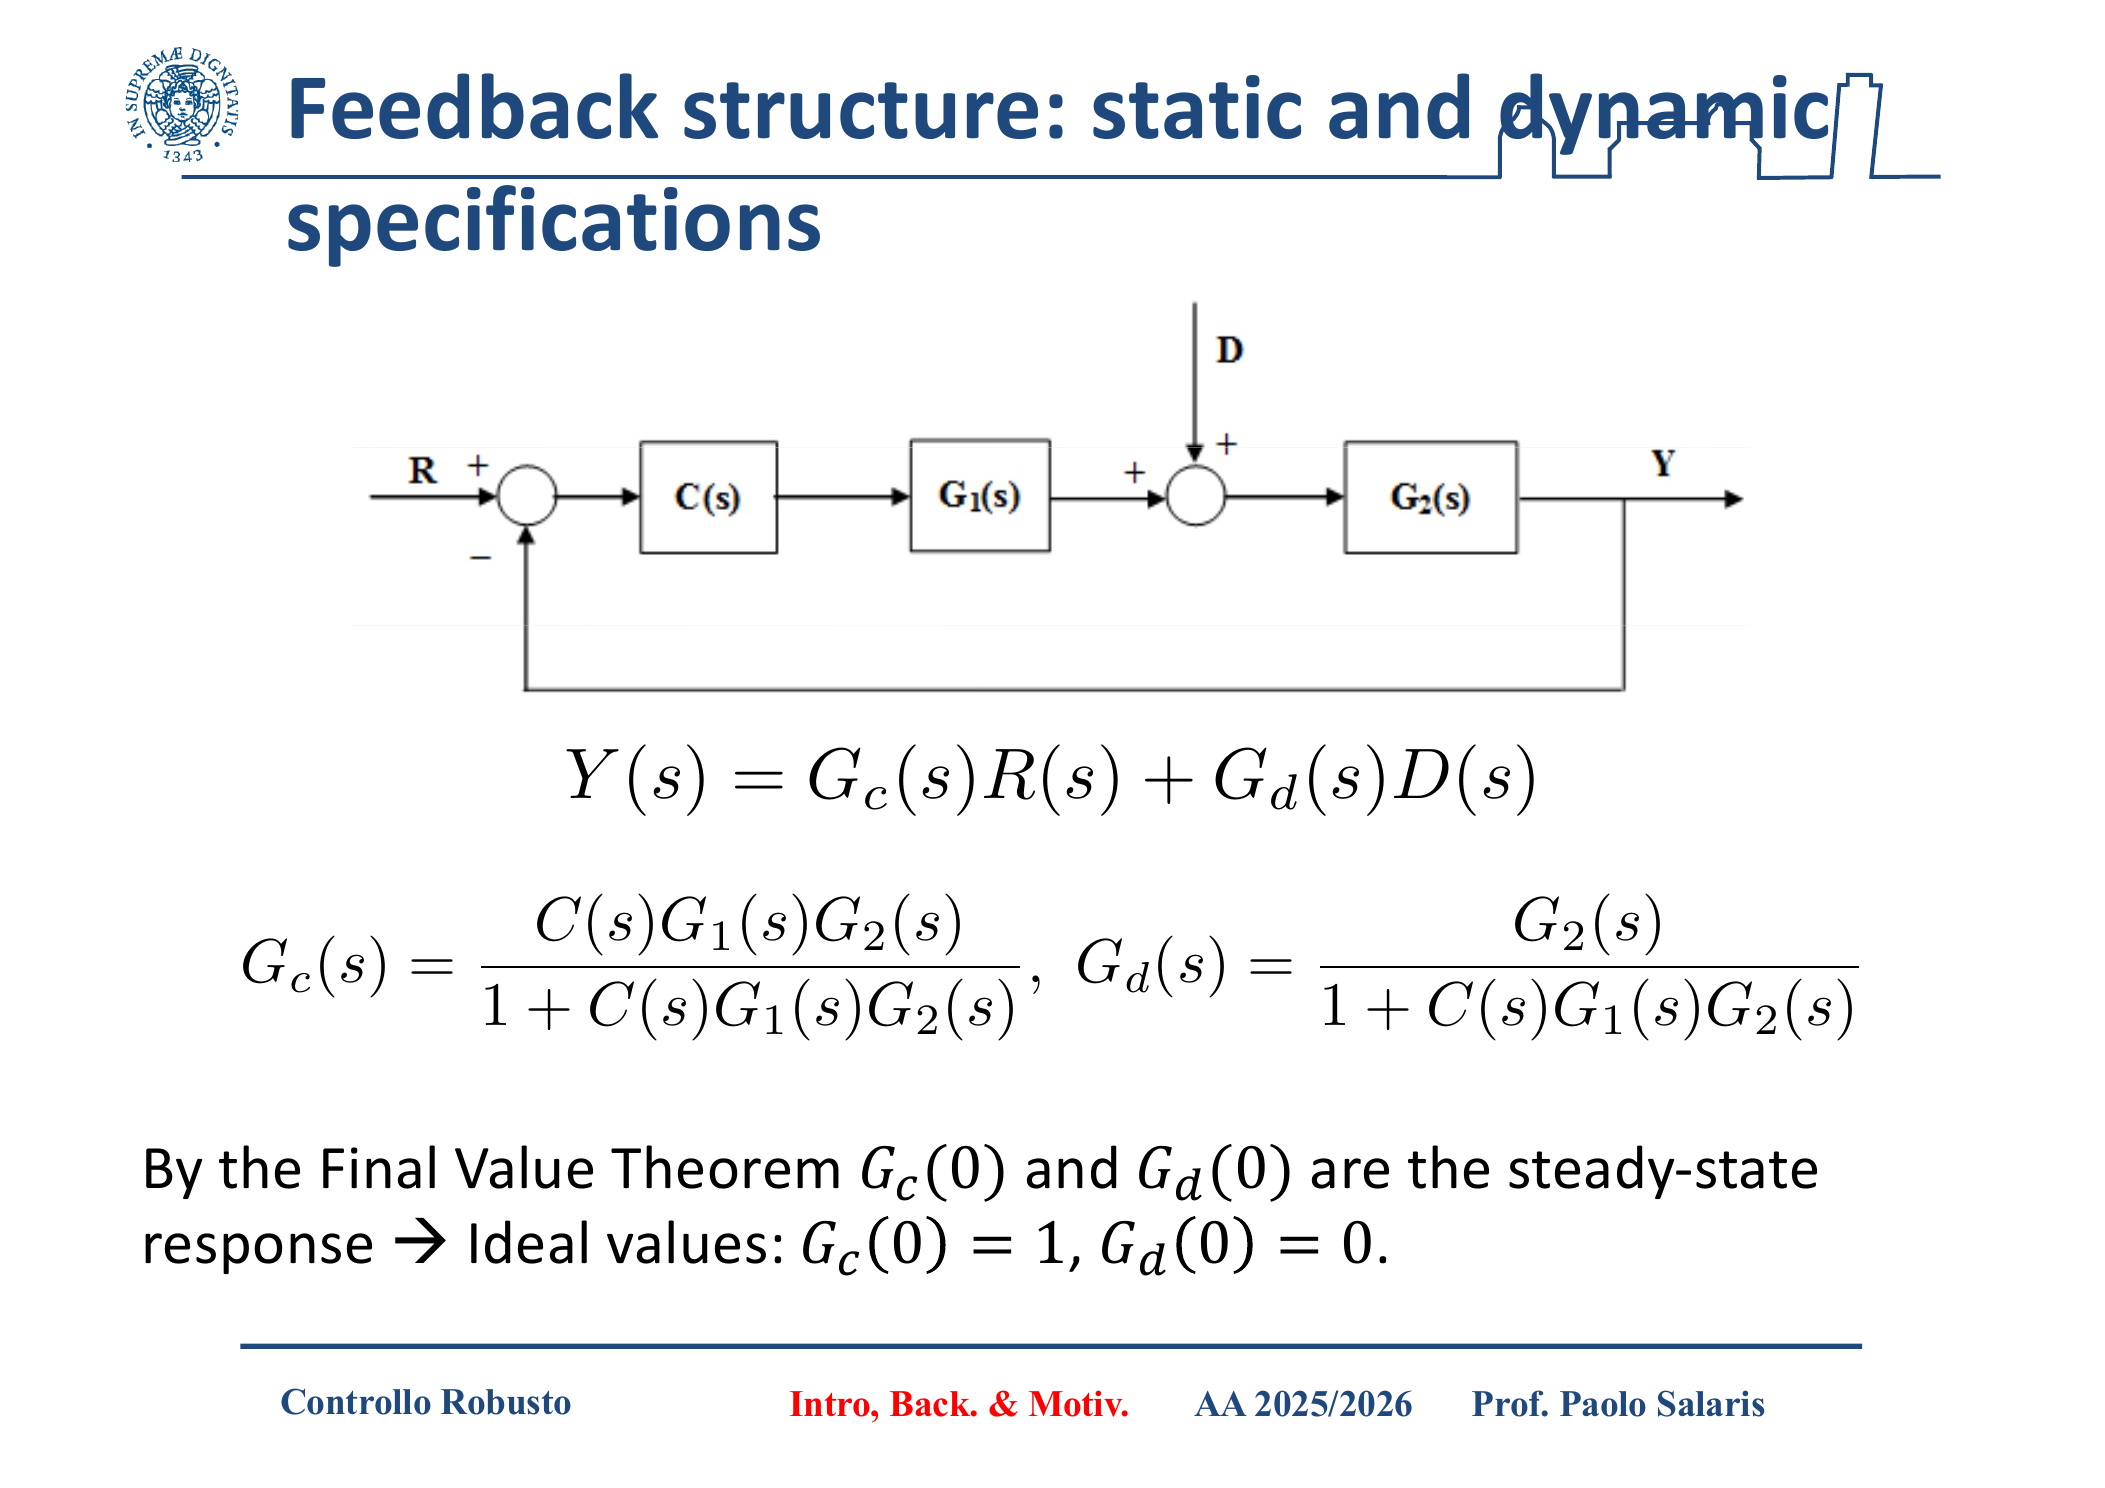
\includegraphics[width=0.76\textwidth]{images2/page-10.png}
    \caption{Definizione delle funzioni $G_c(s)$ e $G_d(s)$ e loro significato a regime.}
\end{figure}

\subsubsection{Errore a regime e tipo del controllore}

La slide 11 applica il teorema del valore finale a due casi fondamentali.

Nel primo caso si prende $R(s)=0$ e un disturbo a gradino $D(s)=1/s$. L'effetto a regime del disturbo viene annullato se il controllore è di tipo 1 o maggiore. Nel secondo caso si prende $R(s)=1/s$ e $D(s)=0$. Anche qui l'errore a regime si annulla se il controllore è di tipo 1 o maggiore.

Dire che il controllore è di \emph{tipo 1} significa che la catena diretta contiene almeno un integratore. Più in generale, il tipo è il numero di poli nell'origine della funzione di trasferimento di anello aperto. Questa nozione è fondamentale perché collega la struttura del controllore alla sua capacità di inseguire segnali polinomiali e rigettare disturbi di bassa frequenza.

In modo intuitivo, l'integratore accumula l'errore nel tempo. Se l'errore permanente fosse non nullo, l'integratore continuerebbe a crescere fino a forzare una correzione del comando. Per questo è un meccanismo naturale per annullare l'errore costante.

\begin{figure}[H]
    \centering
    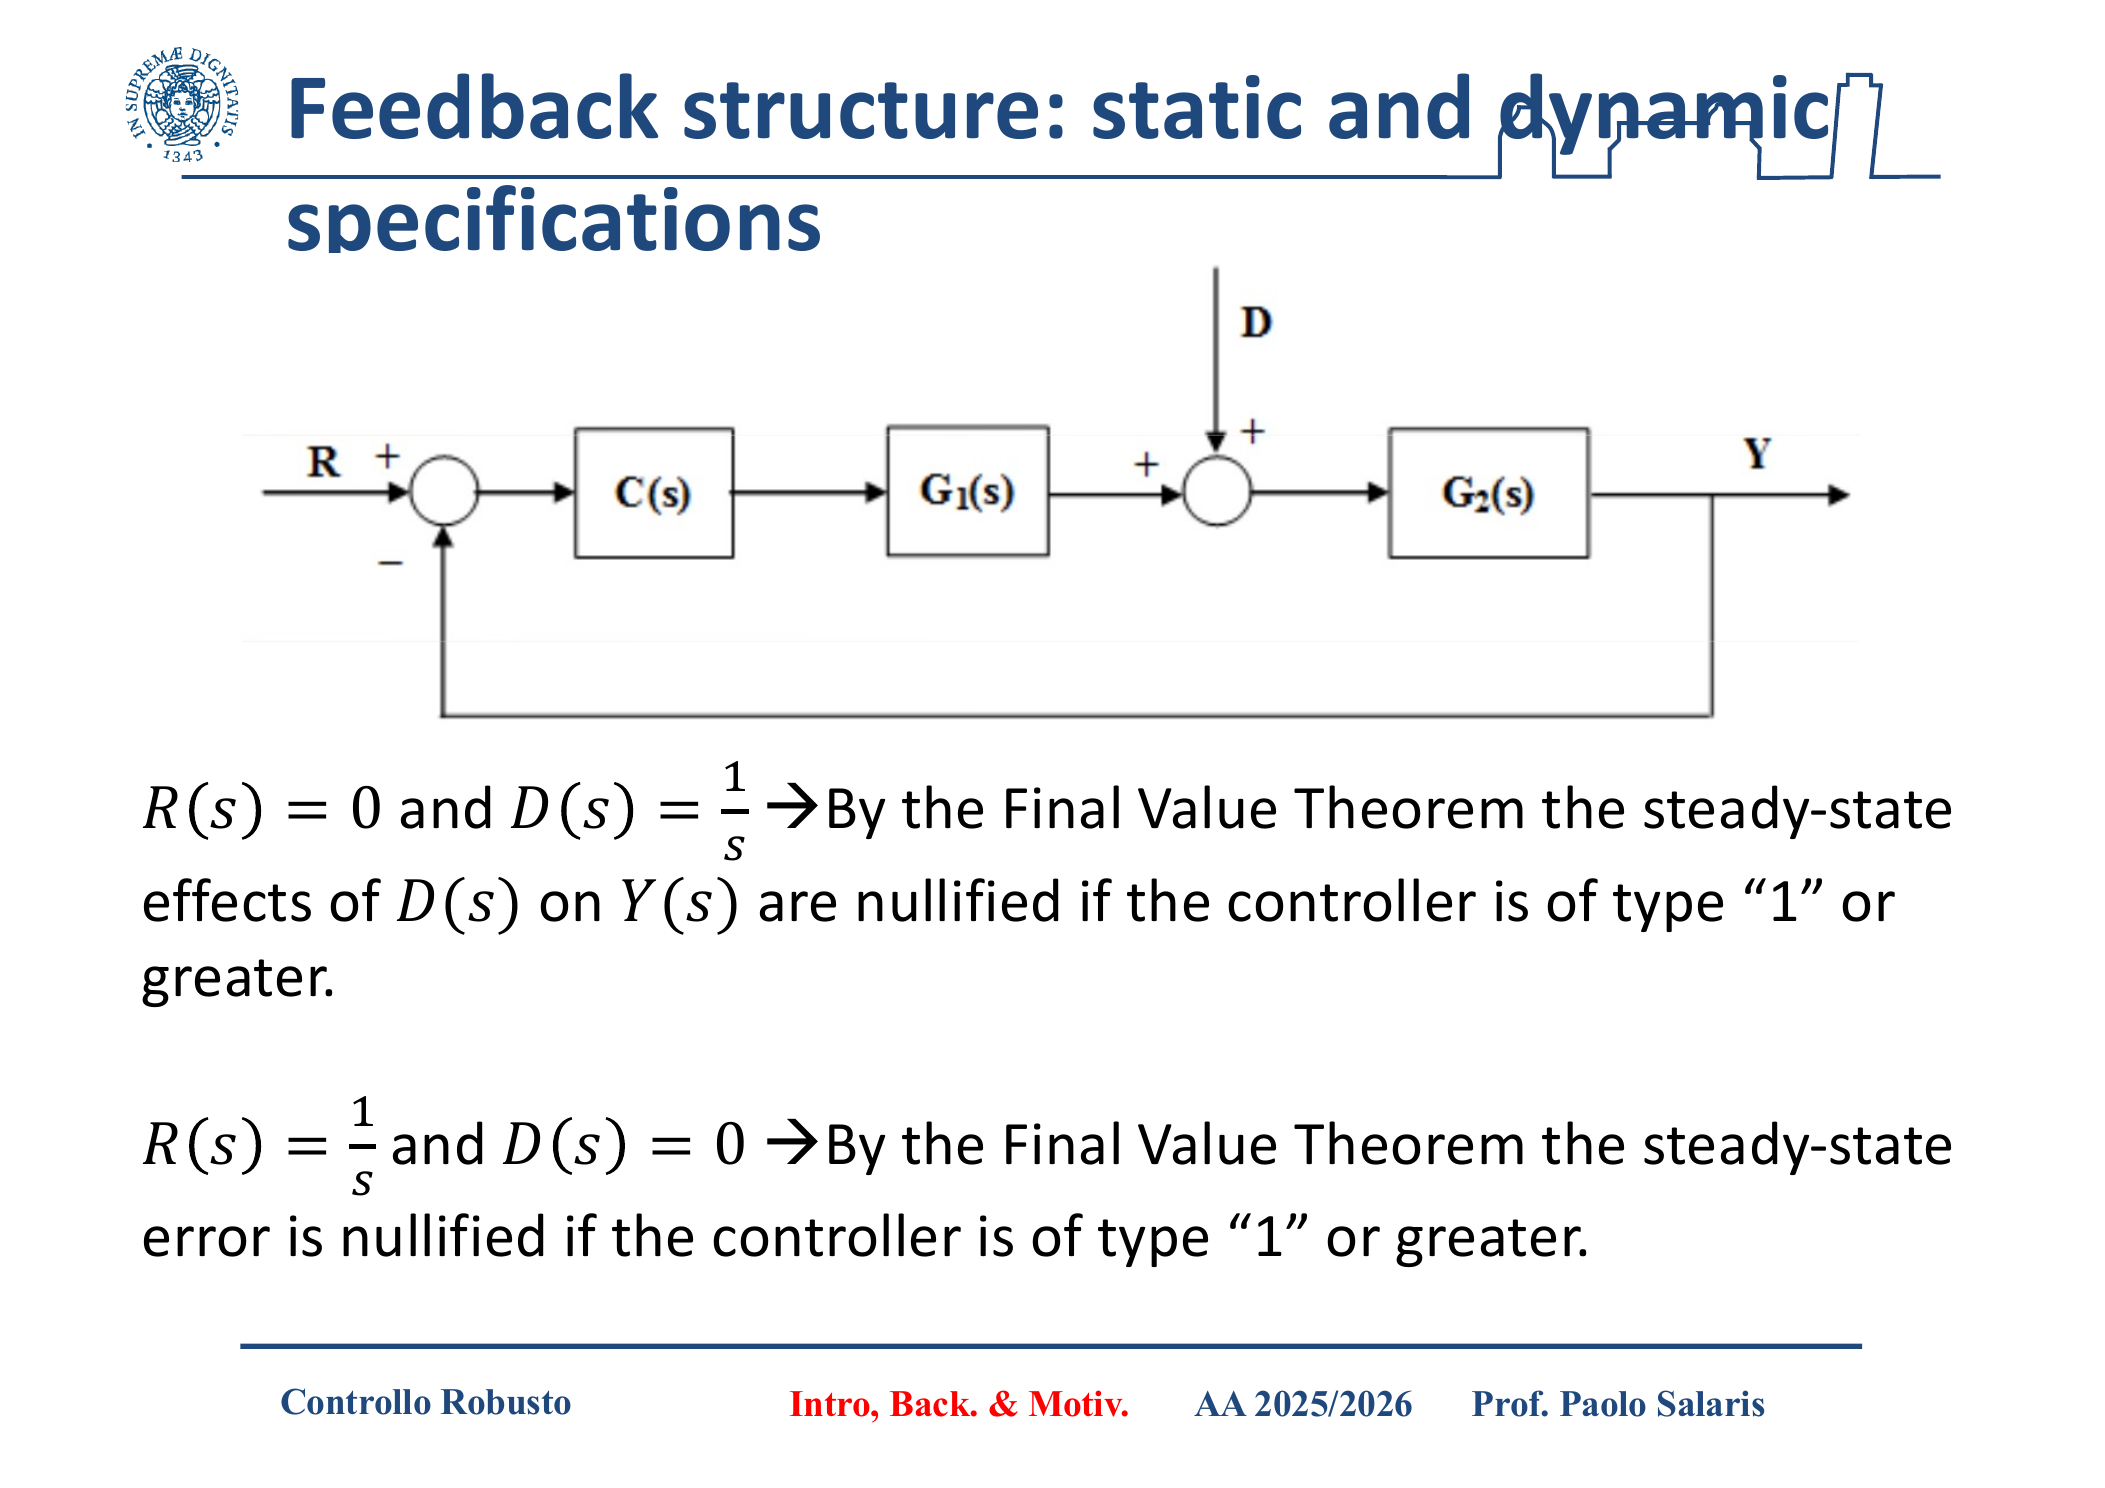
\includegraphics[width=0.76\textwidth]{images2/page-11.png}
    \caption{Condizioni sufficienti per annullare a regime un gradino di riferimento o un gradino di disturbo.}
\end{figure}

\subsubsection{Principio del modello interno}

La slide 12 riassume il senso profondo di questo risultato nel \emph{principio del modello interno}. La traduzione concettuale è la seguente.

Per avere errore nullo a regime in risposta a un certo ingresso, la catena diretta $C(s)P(s)$ deve essere in grado di generare un modo dinamico uguale al modo del segnale di ingresso. Se il segnale è costante, il modo da riprodurre è quello associato a un polo nell'origine. Se il segnale fosse una rampa, servirebbero due integratori, e così via.

Per il rigetto di disturbi a regime la logica è analoga. Il modo caratteristico del disturbo deve comparire nei blocchi a monte del punto di iniezione del disturbo stesso. Questa formulazione è estremamente importante in controllo robusto, perché spiega perché certe prestazioni statiche non possono essere ottenute arbitrariamente: devono essere supportate dalla struttura dinamica del controllore.

\begin{figure}[H]
    \centering
    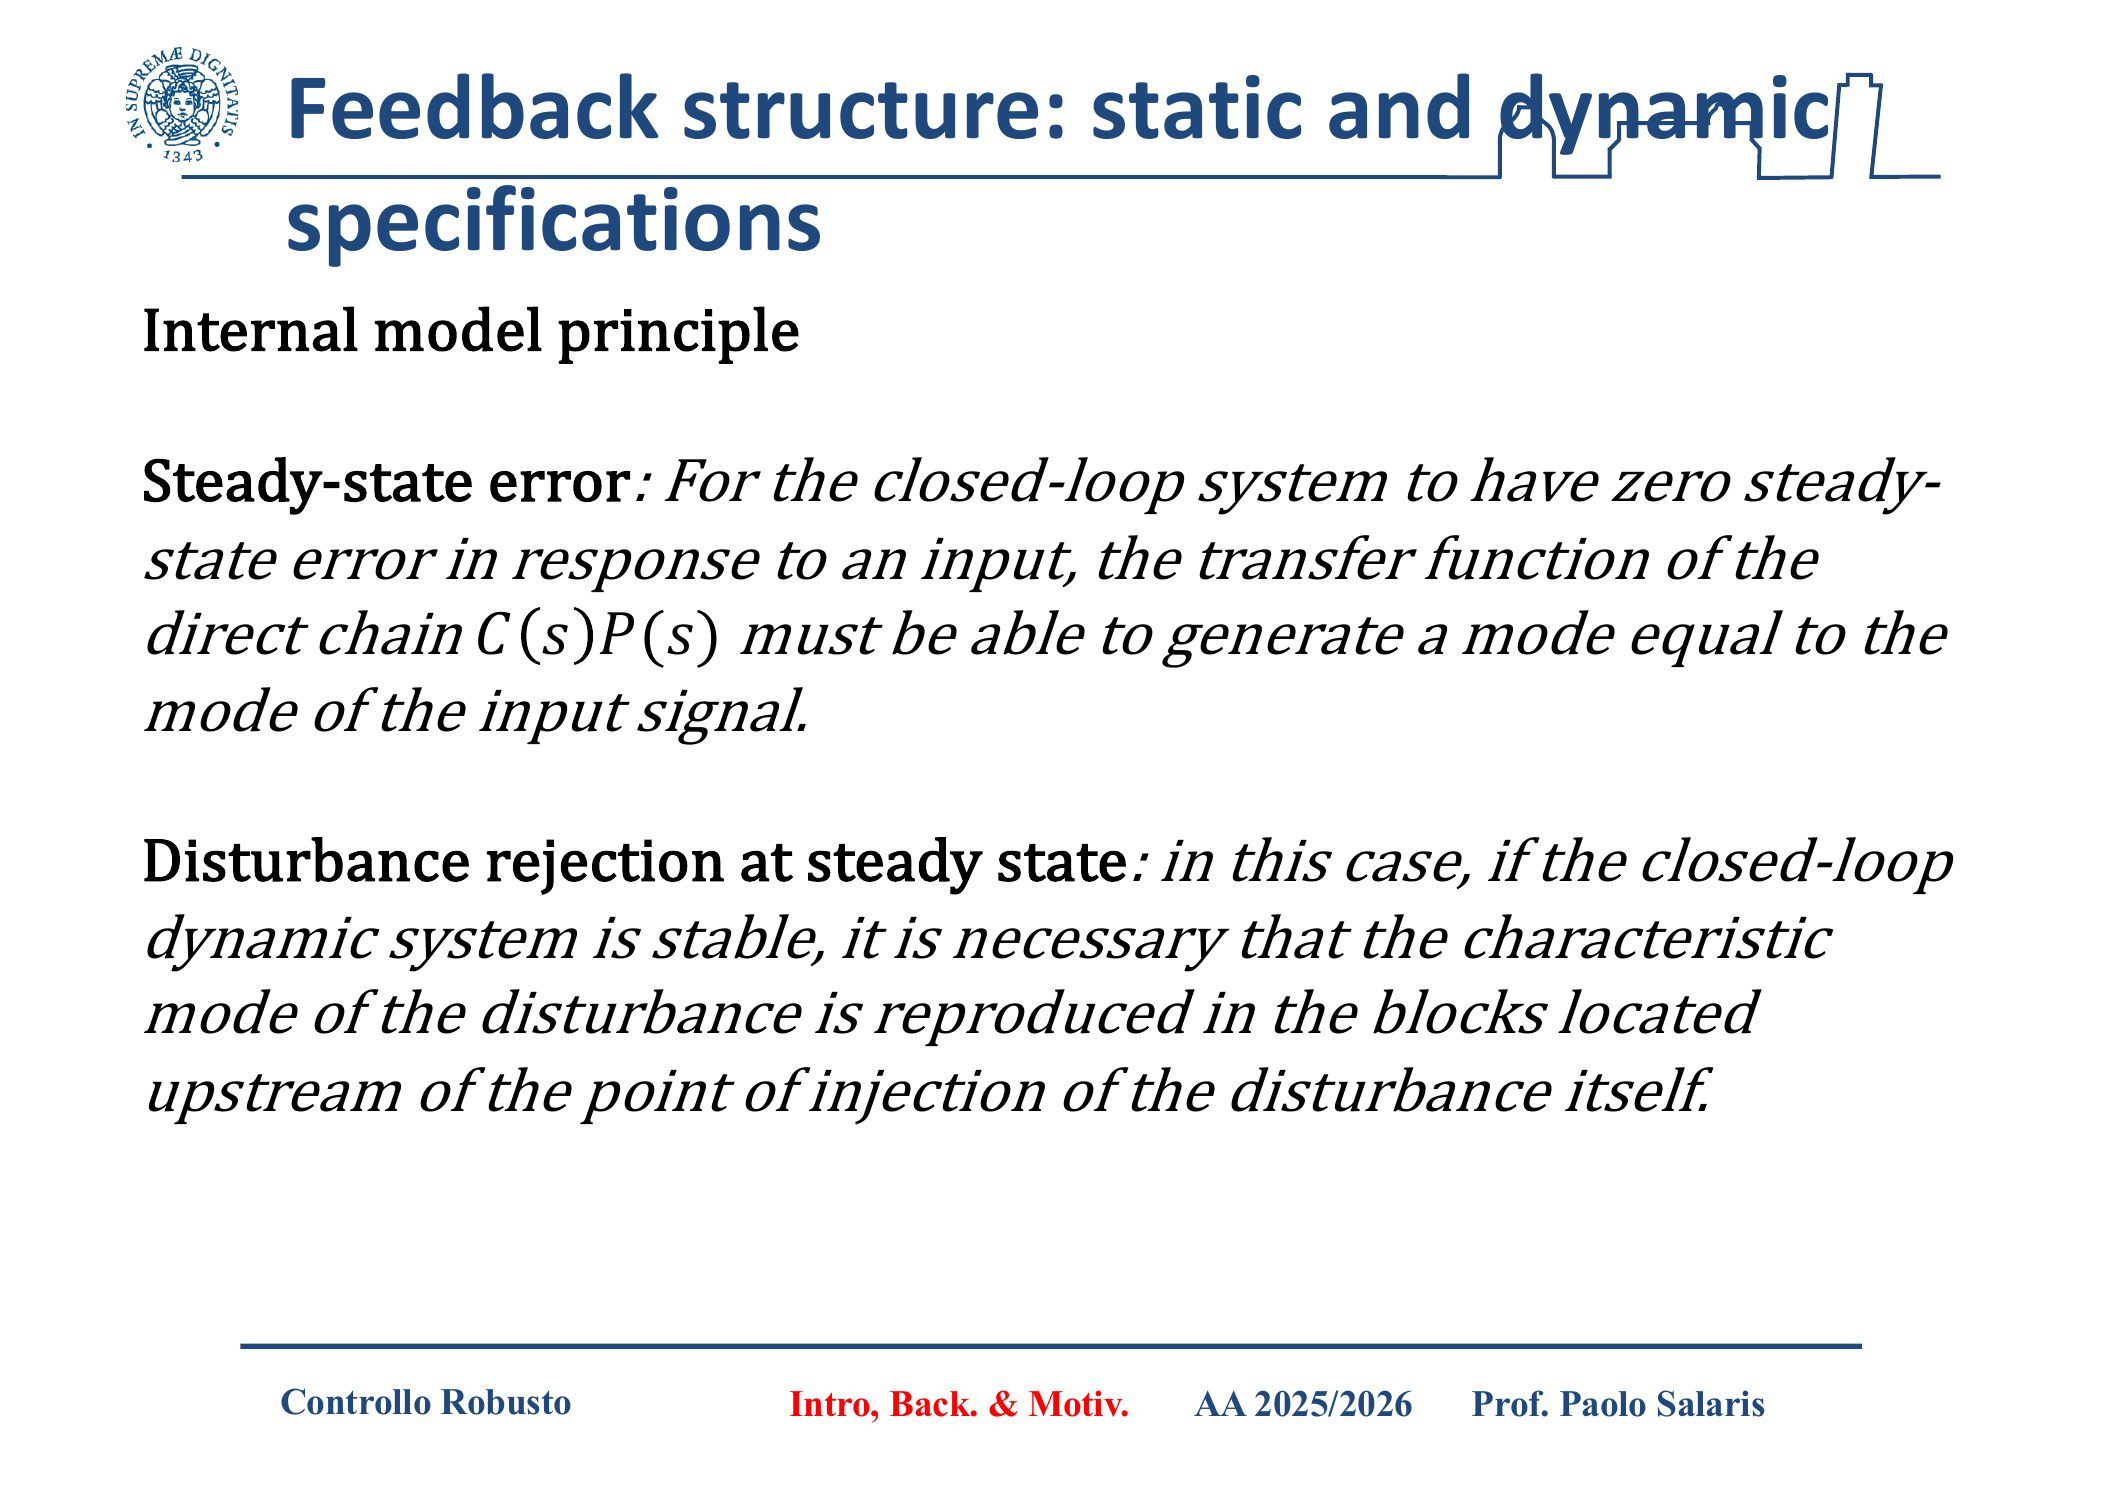
\includegraphics[width=0.78\textwidth]{images2/page-12.png}
    \caption{Slide sul principio del modello interno.}
\end{figure}

\begin{keybox}
Il principio del modello interno dice che un segnale si può inseguire o rigettare a regime solo se la dinamica che lo genera è incorporata nella catena di controllo nel punto corretto della struttura. Non è un dettaglio tecnico: è un vincolo strutturale del problema.
\end{keybox}

\subsubsection{Specifiche dinamiche nel dominio del tempo}

La slide 13 introduce tre misure classiche del transitorio:
\begin{enumerate}
    \item tempo di salita;
    \item tempo di assestamento, tipicamente al 5\% o al 2\%;
    \item sovraelongazione massima.
\end{enumerate}

Il tempo di salita misura quanto rapidamente l'uscita raggiunge il valore desiderato. Il tempo di assestamento misura quanto rapidamente la risposta entra e resta entro una fascia intorno al valore finale. La sovraelongazione misura quanto il transitorio supera il valore finale prima di smorzarsi.

Questi tre indicatori sono spesso in competizione. Aumentare la rapidità tende a richiedere una banda passante maggiore e spesso riduce lo smorzamento. Aumentare lo smorzamento riduce l'overshoot ma può rallentare la risposta. Una buona sintesi robusta deve bilanciare questi effetti senza perdere margini di stabilità o aumentare eccessivamente la sensibilità al rumore.

\begin{figure}[H]
    \centering
    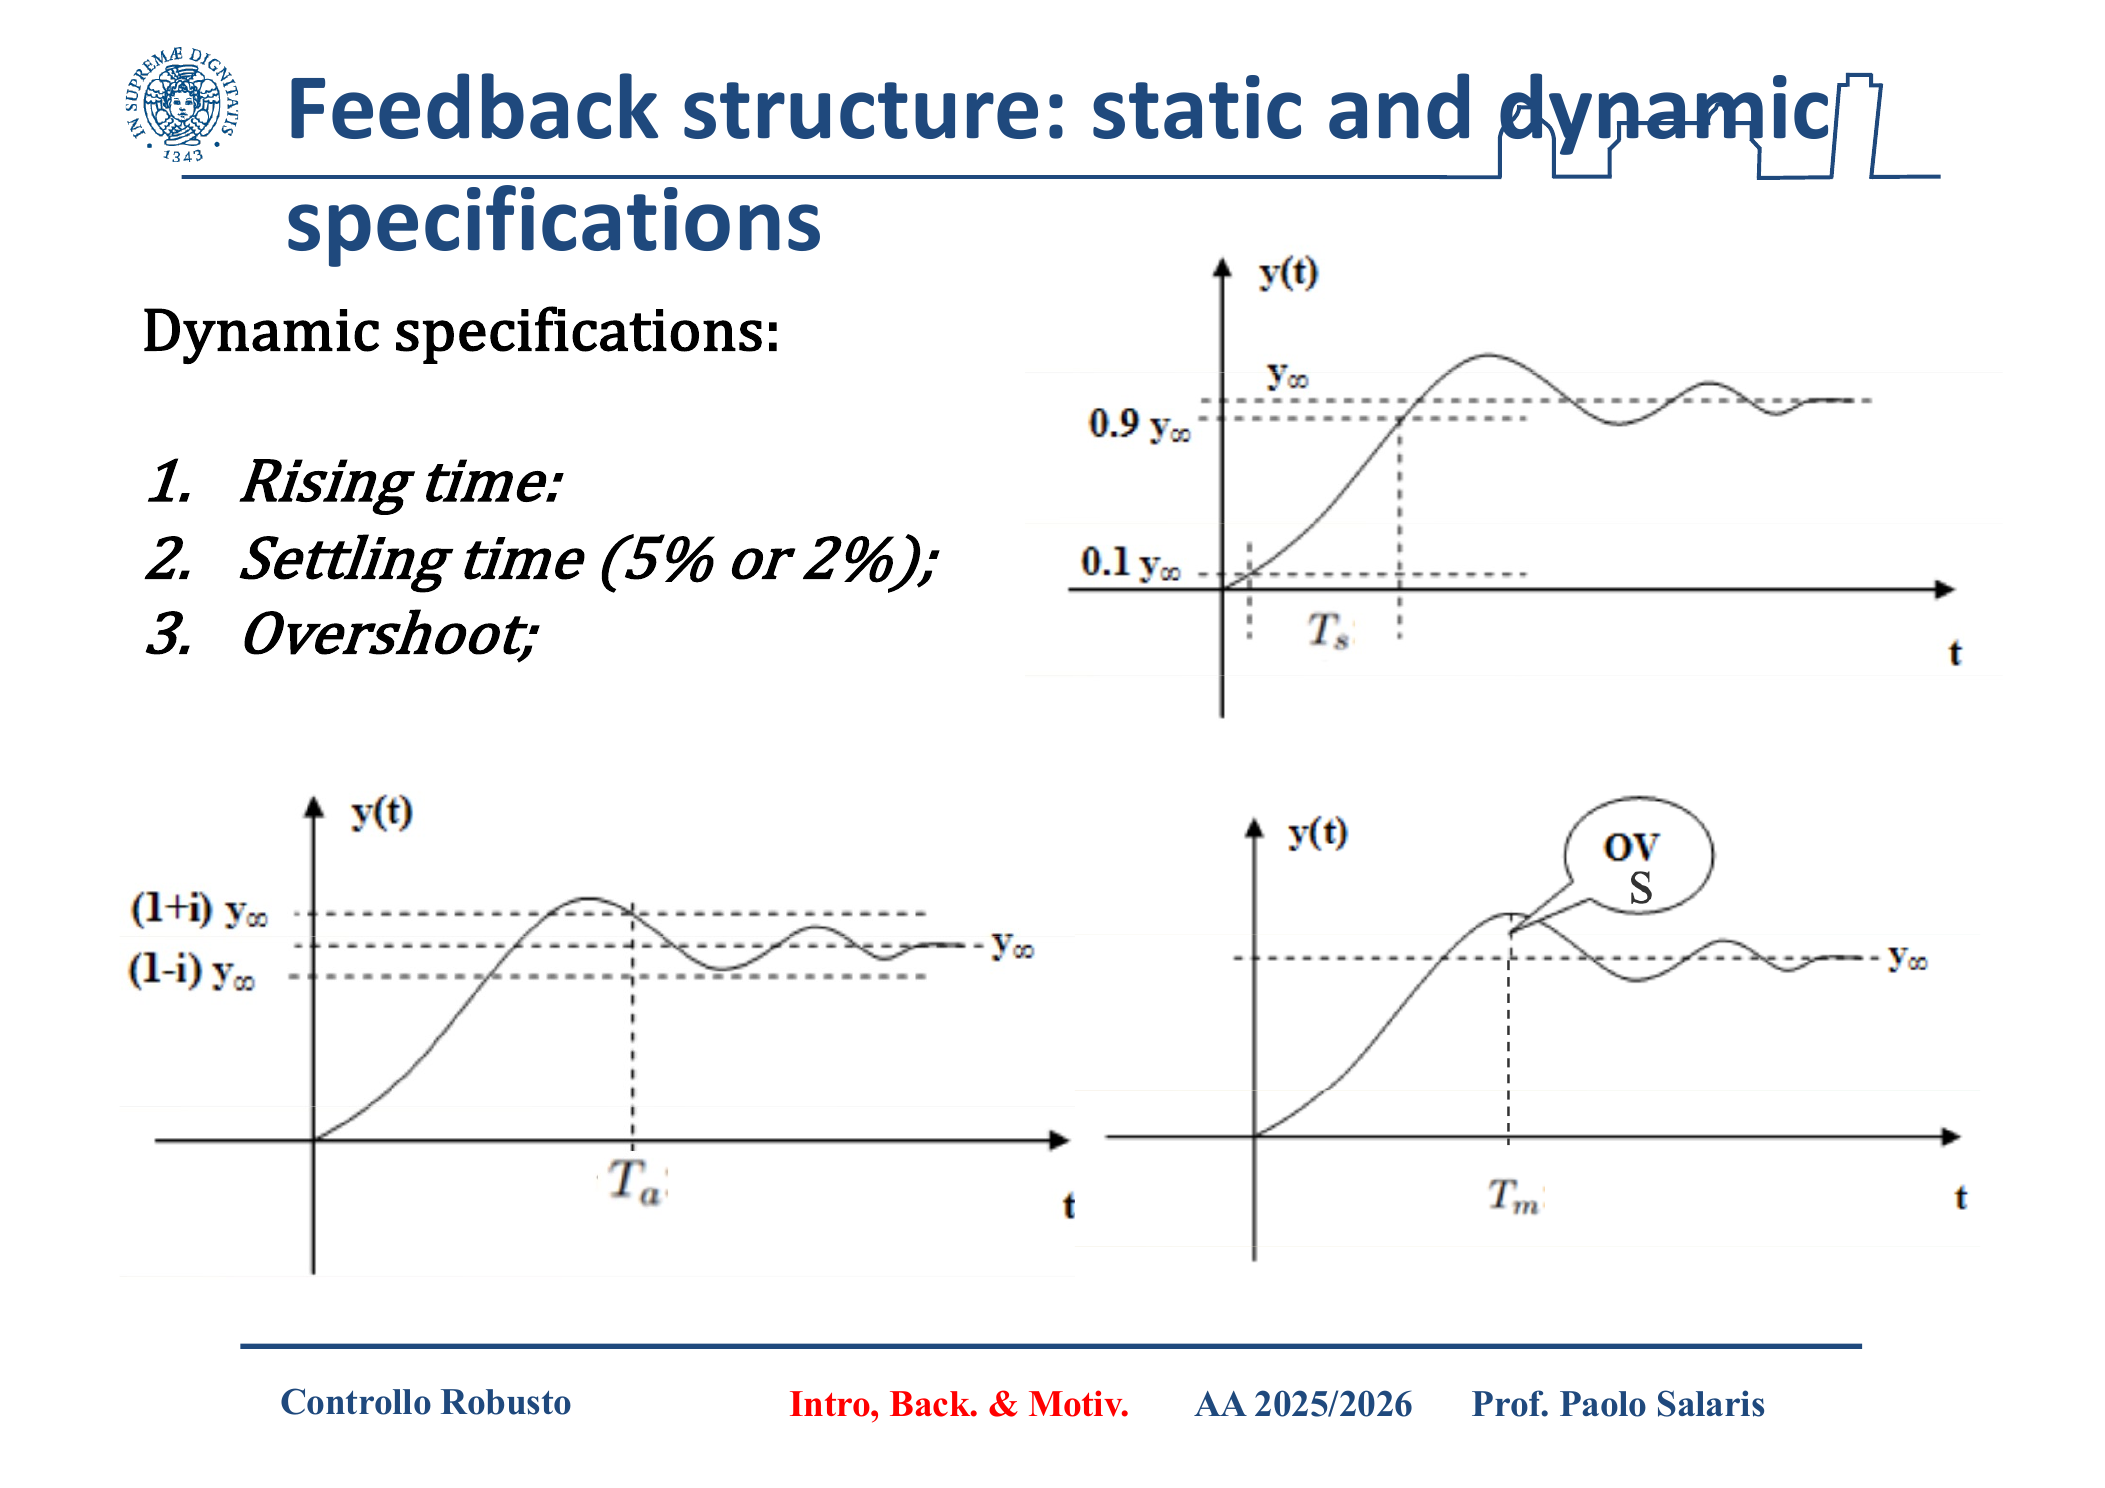
\includegraphics[width=0.82\textwidth]{images2/page-13.png}
    \caption{Definizioni grafiche di tempo di salita, tempo di assestamento e sovraelongazione.}
\end{figure}

\subsubsection{Relazioni tempo-frequenza}

La slide 14 apre il collegamento fra prestazioni nel tempo e prestazioni in frequenza. Per la funzione di trasferimento chiusa
$$
G_c(s)=\frac{K(s)P(s)}{1+K(s)P(s)},
$$
si ha, in frequenza,
$$
|G_c(j\omega)|=\frac{|K(j\omega)P(j\omega)|}{|1+K(j\omega)P(j\omega)|}.
$$

Alle basse frequenze, quando $|K(j\omega)P(j\omega)|\gg1$, il sistema chiuso tende a inseguire bene il riferimento e si ha approssimativamente $|G_c(j\omega)|\approx1$. Alle alte frequenze, quando il guadagno d'anello scende, la risposta chiusa tende invece a seguire il comportamento dell'anello aperto. La frequenza di attraversamento $\omega_T$ diventa così un indicatore sintetico della rapidità del sistema.

In prima approssimazione, una frequenza di attraversamento più alta corrisponde a un transitorio più rapido, cioè a un tempo di salita più piccolo. Ma un aumento eccessivo di $\omega_T$ può compromettere lo smorzamento o i margini di fase, per cui il legame non va letto in modo ingenuo.

\begin{figure}[H]
    \centering
    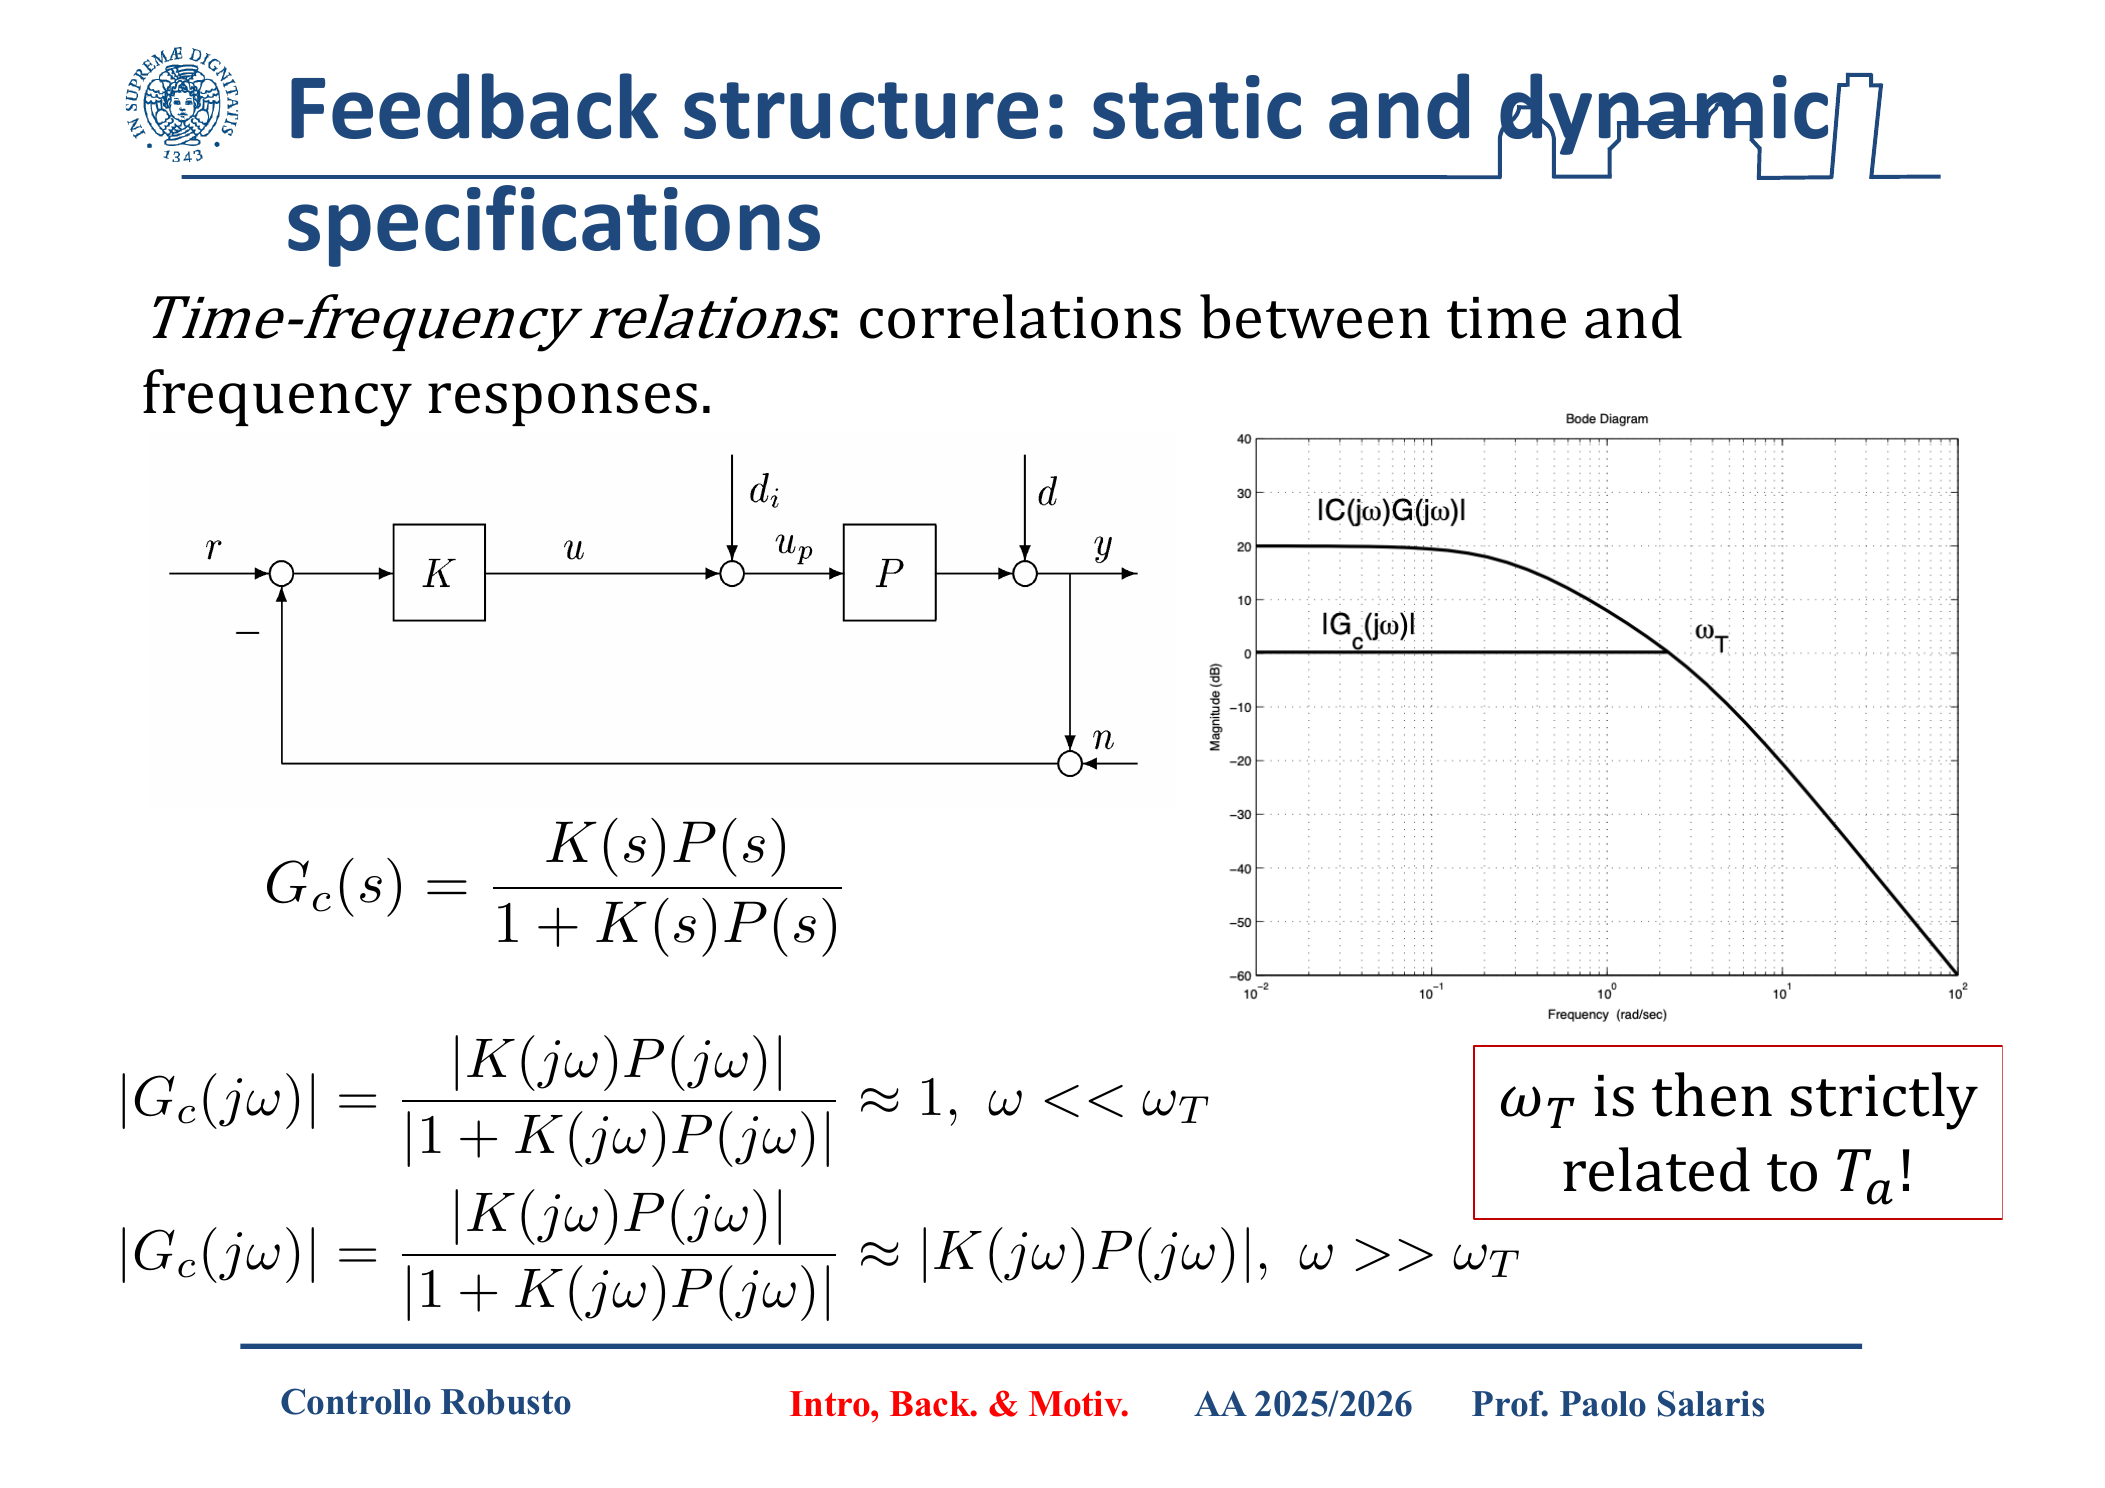
\includegraphics[width=0.82\textwidth]{images2/page-14.png}
    \caption{Prima relazione tempo-frequenza: la frequenza di attraversamento $\omega_T$ è strettamente legata alla rapidità del transitorio.}
\end{figure}

\subsubsection{Ruolo del margine di fase}

Le slide 15 e 16 analizzano il comportamento esattamente in corrispondenza di $\omega=\omega_T$, dove $|K(j\omega_T)P(j\omega_T)|=1$. Se la fase di anello aperto in quel punto è
$$
\arg(K(j\omega_T)P(j\omega_T))=-\pi+M_f,
$$
allora il modulo della funzione chiusa vale
$$
|G_c(j\omega_T)|=\frac{1}{2\sin(M_f/2)}.
$$

Questa formula è importante perché collega direttamente il \emph{margine di fase} $M_f$ a una misura della risonanza del chiuso e quindi alla forma del transitorio. Se il margine di fase è piccolo, il denominatore $2\sin(M_f/2)$ è piccolo e il modulo di $G_c(j\omega_T)$ aumenta: ciò significa maggiore amplificazione vicino alla banda passante e, tipicamente, maggiore overshoot nel dominio del tempo. Se invece il margine di fase cresce, la risposta tende a essere più smorzata.

La slide richiama anche due approssimazioni classiche:
\begin{itemize}
    \item per $M_f\approx\SI{90}{\degree}$, il chiuso si comporta in modo vicino a un primo ordine con costante di tempo $\tau\approx1/\omega_T$;
    \item per margini di fase più piccoli, il comportamento si avvicina meglio a un secondo ordine con pulsazione naturale vicina a $\omega_T$ e coefficiente di smorzamento legato a $M_f$.
\end{itemize}

Da qui derivano stime pratiche come
$$
T_{a,5\%}\approx\frac{3}{\omega_T}
\quad \text{oppure} \quad
T_{a,5\%}\approx\frac{3}{\zeta\omega_T},
$$
a seconda del modello approssimante adottato.

\begin{figure}[H]
    \centering
    \begin{subfigure}{0.49\textwidth}
        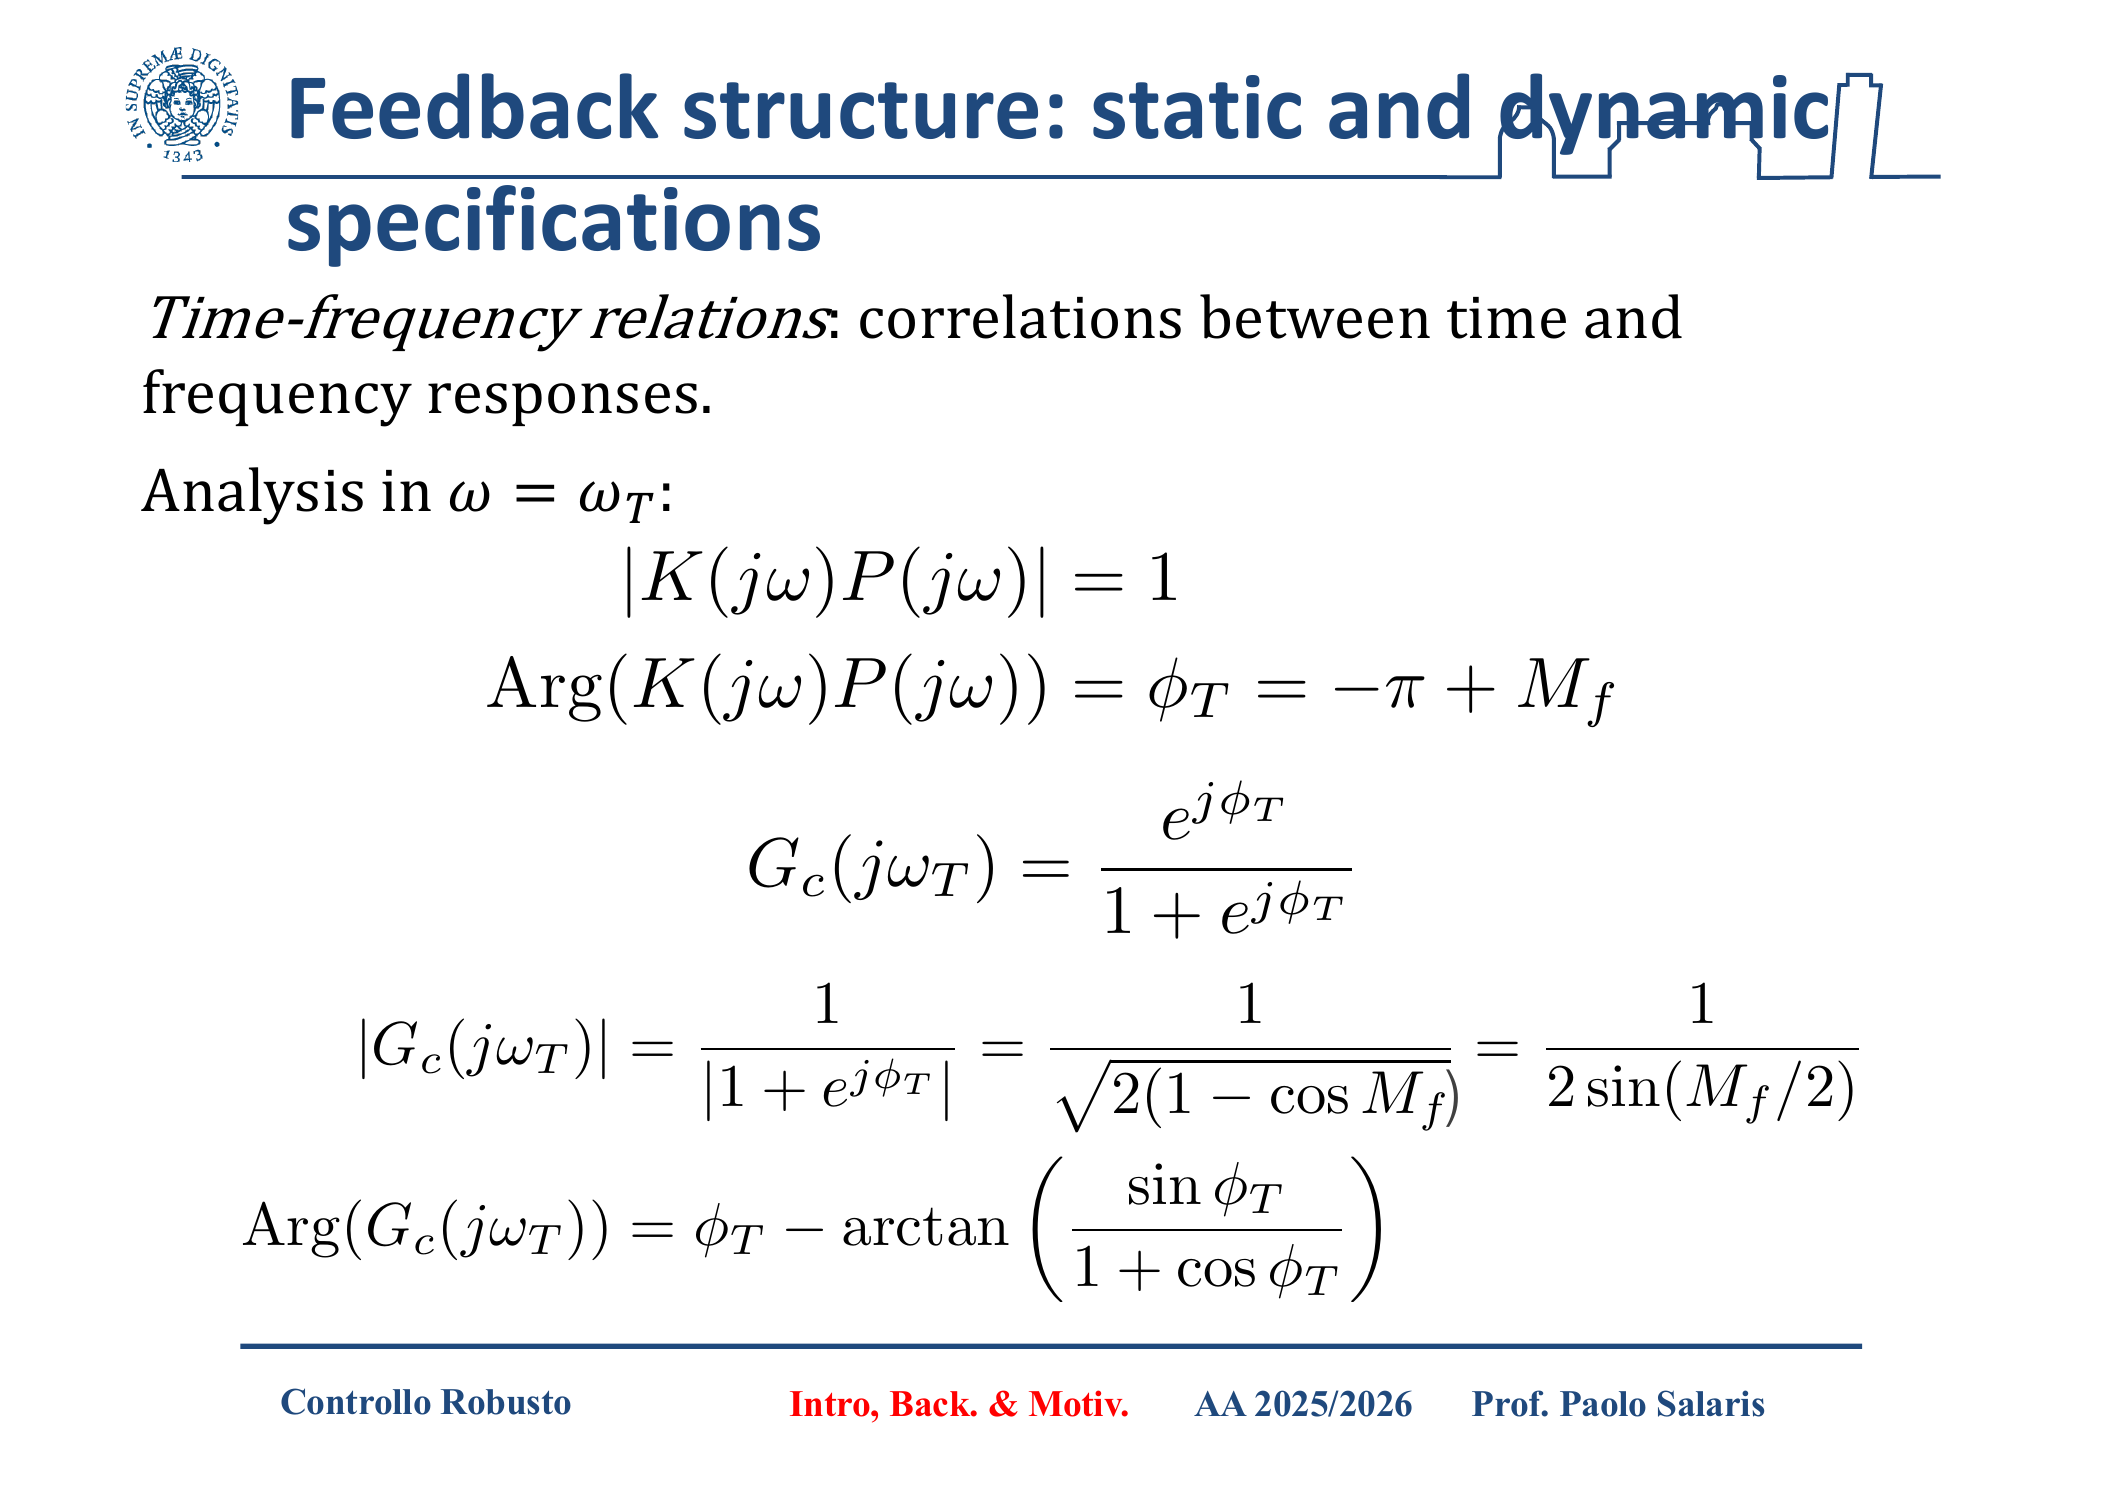
\includegraphics[width=\linewidth]{images2/page-15.png}
        \caption{Analisi in $\omega=\omega_T$.}
    \end{subfigure}
    \hfill
    \begin{subfigure}{0.49\textwidth}
        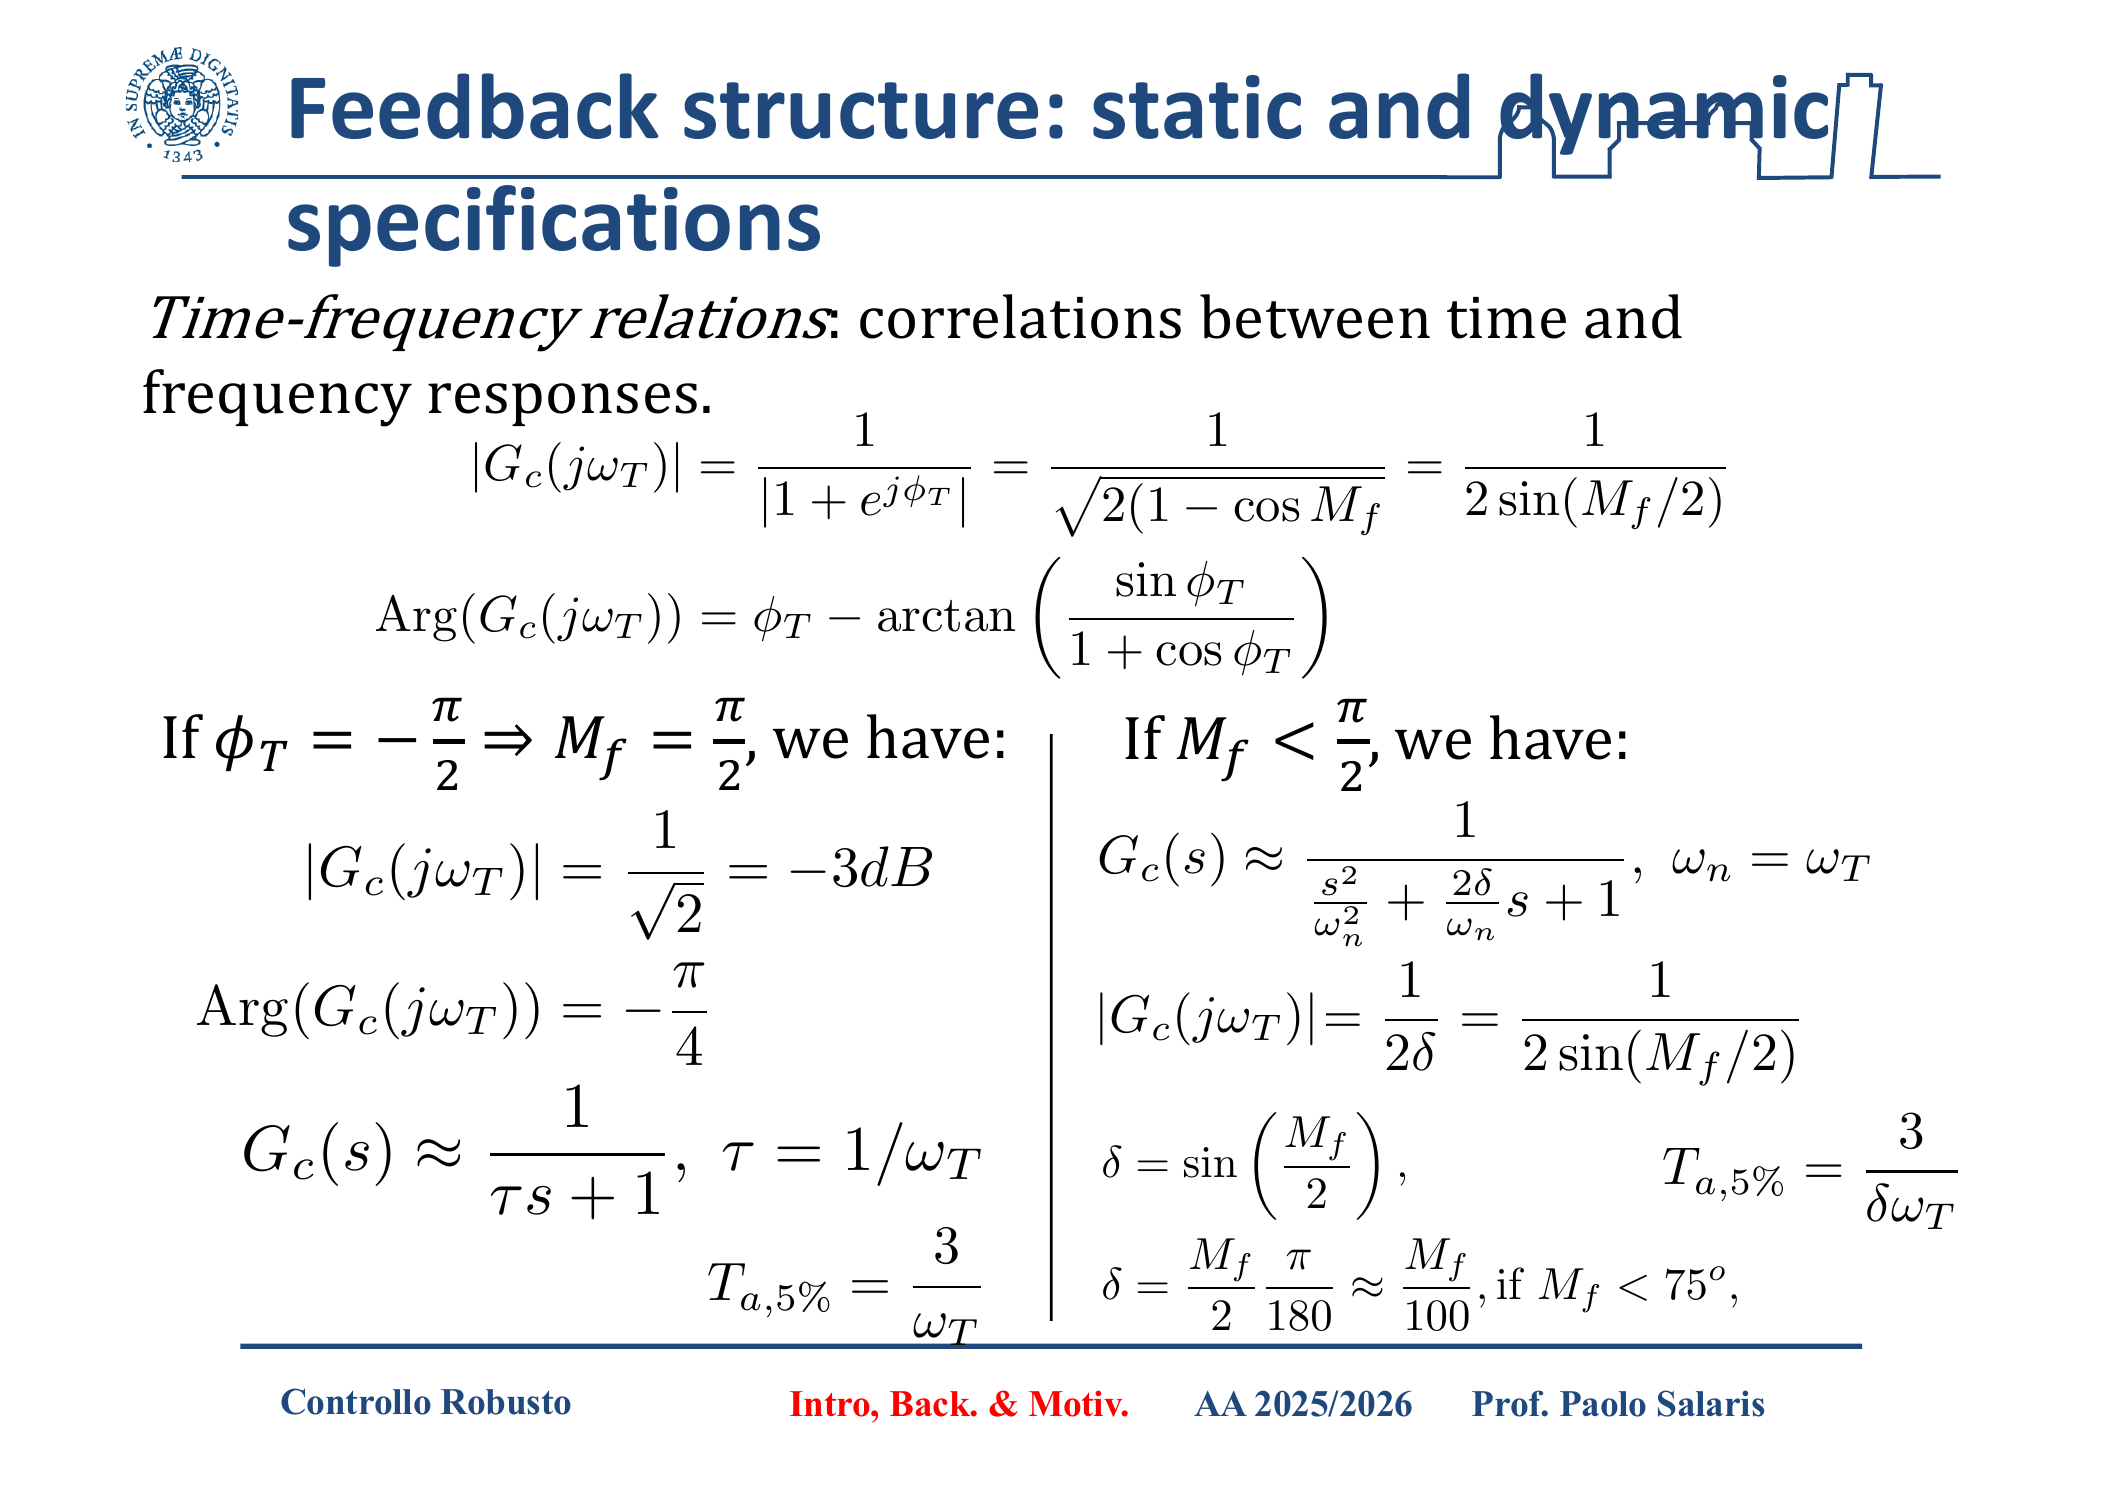
\includegraphics[width=\linewidth]{images2/page-16.png}
        \caption{Legame fra modulo in attraversamento, margine di fase e transitorio.}
    \end{subfigure}
    \caption{Le relazioni tempo-frequenza permettono di collegare $\omega_T$ e $M_f$ a rapidità e smorzamento.}
\end{figure}

\subsection{Sensitività e robustezza rispetto alle incertezze parametriche}

\subsubsection{Perché introdurre la sensitività}

Il blocco finale delle slide confronta uno schema feed-forward con uno schema feedback e si chiede: \emph{quanto cambia l'uscita quando un parametro del processo cambia rispetto al valore nominale?} Questa è esattamente la domanda che porta alla sensitività.

Si considera un parametro fisico significativo, indicato con $\alpha$, con valore nominale $\hat\alpha$ e perturbazione $\delta\alpha$:
$$
\alpha=\hat\alpha+\delta\alpha.
$$
L'impianto reale viene scritto come
$$
P_p(s)=P(s,\hat\alpha)+\Delta P(s)=P_p(\alpha,s).
$$

Nel caso feed-forward l'uscita nominale è
$$
\hat Y(s)=K_{ff}C_{ff}(s)P(\hat\alpha,s)R(s),
$$
mentre quella perturbata è
$$
Y(s)=K_{ff}C_{ff}(s)P(\alpha,s)R(s).
$$
Questo set-up permette di quantificare in modo pulito il peso dell'errore di modello.

\begin{figure}[H]
    \centering
    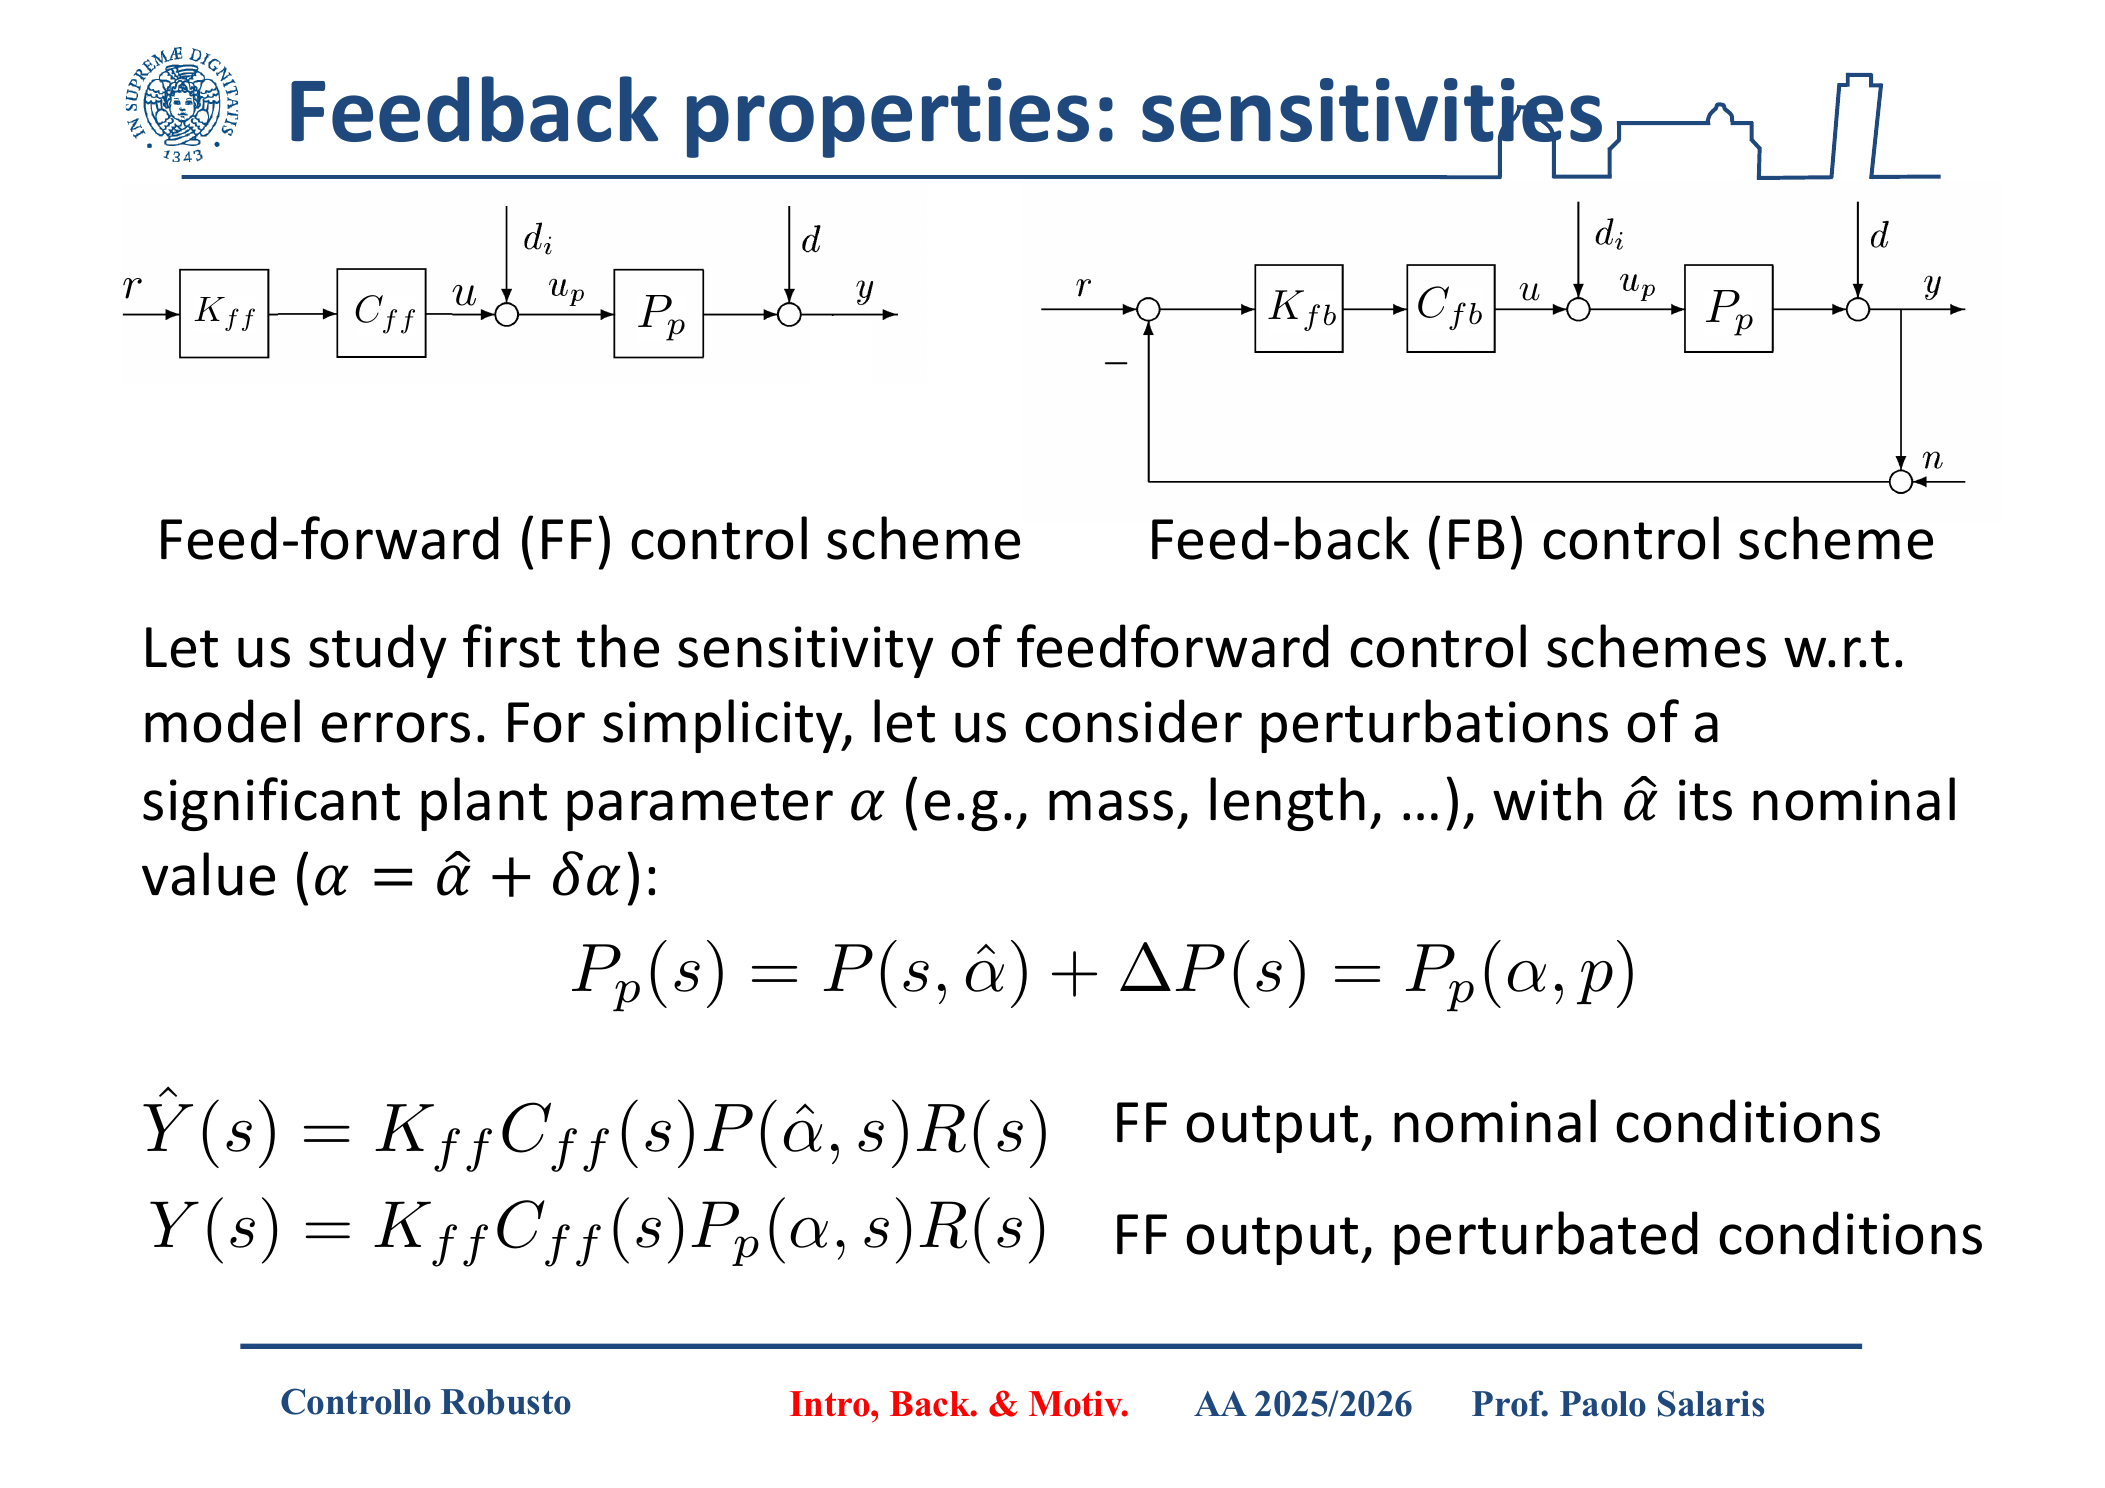
\includegraphics[width=0.82\textwidth]{images2/page-17.png}
    \caption{Confronto fra schema feed-forward e schema feedback per introdurre la sensitività ai parametri dell'impianto.}
\end{figure}

\subsubsection{Sensitività dell'impianto}

Le slide definiscono la variazione relativa di uscita nello schema feed-forward come
$$
\frac{\Delta Y(s)}{\hat Y(s)}=
\frac{Y(s)-\hat Y(s)}{\hat Y(s)}=
\frac{P_p(\alpha,s)-P(\hat\alpha,s)}{P(\hat\alpha,s)}=
\frac{\Delta P(s)}{P(s)}.
$$
Per piccole variazioni di parametro si linearizza questa quantità rispetto a $\alpha$ e si ottiene
$$
\frac{\Delta P(s)}{P(s)}\approx
\left[\left.\frac{\partial P_p(\alpha,s)}{\partial \alpha}\right|_{\hat\alpha}
\frac{\hat\alpha}{P(\hat\alpha,s)}\right]
\frac{\Delta\alpha}{\hat\alpha}
= S_{\alpha,o}(s)\frac{\Delta\alpha}{\hat\alpha}.
$$
La quantità
$$
S_{\alpha,o}(s)
$$
è la \emph{sensitività dell'impianto} rispetto al parametro $\alpha$. Essa misura quanta variazione relativa di modello si ottiene per una certa variazione relativa del parametro.

Questa definizione è importante perché separa due contributi:
\begin{itemize}
    \item l'entità dell'incertezza fisica, cioè $\Delta\alpha/\hat\alpha$;
    \item la sensibilità intrinseca della dinamica rispetto a quel parametro, cioè $S_{\alpha,o}(s)$.
\end{itemize}

\begin{figure}[H]
    \centering
    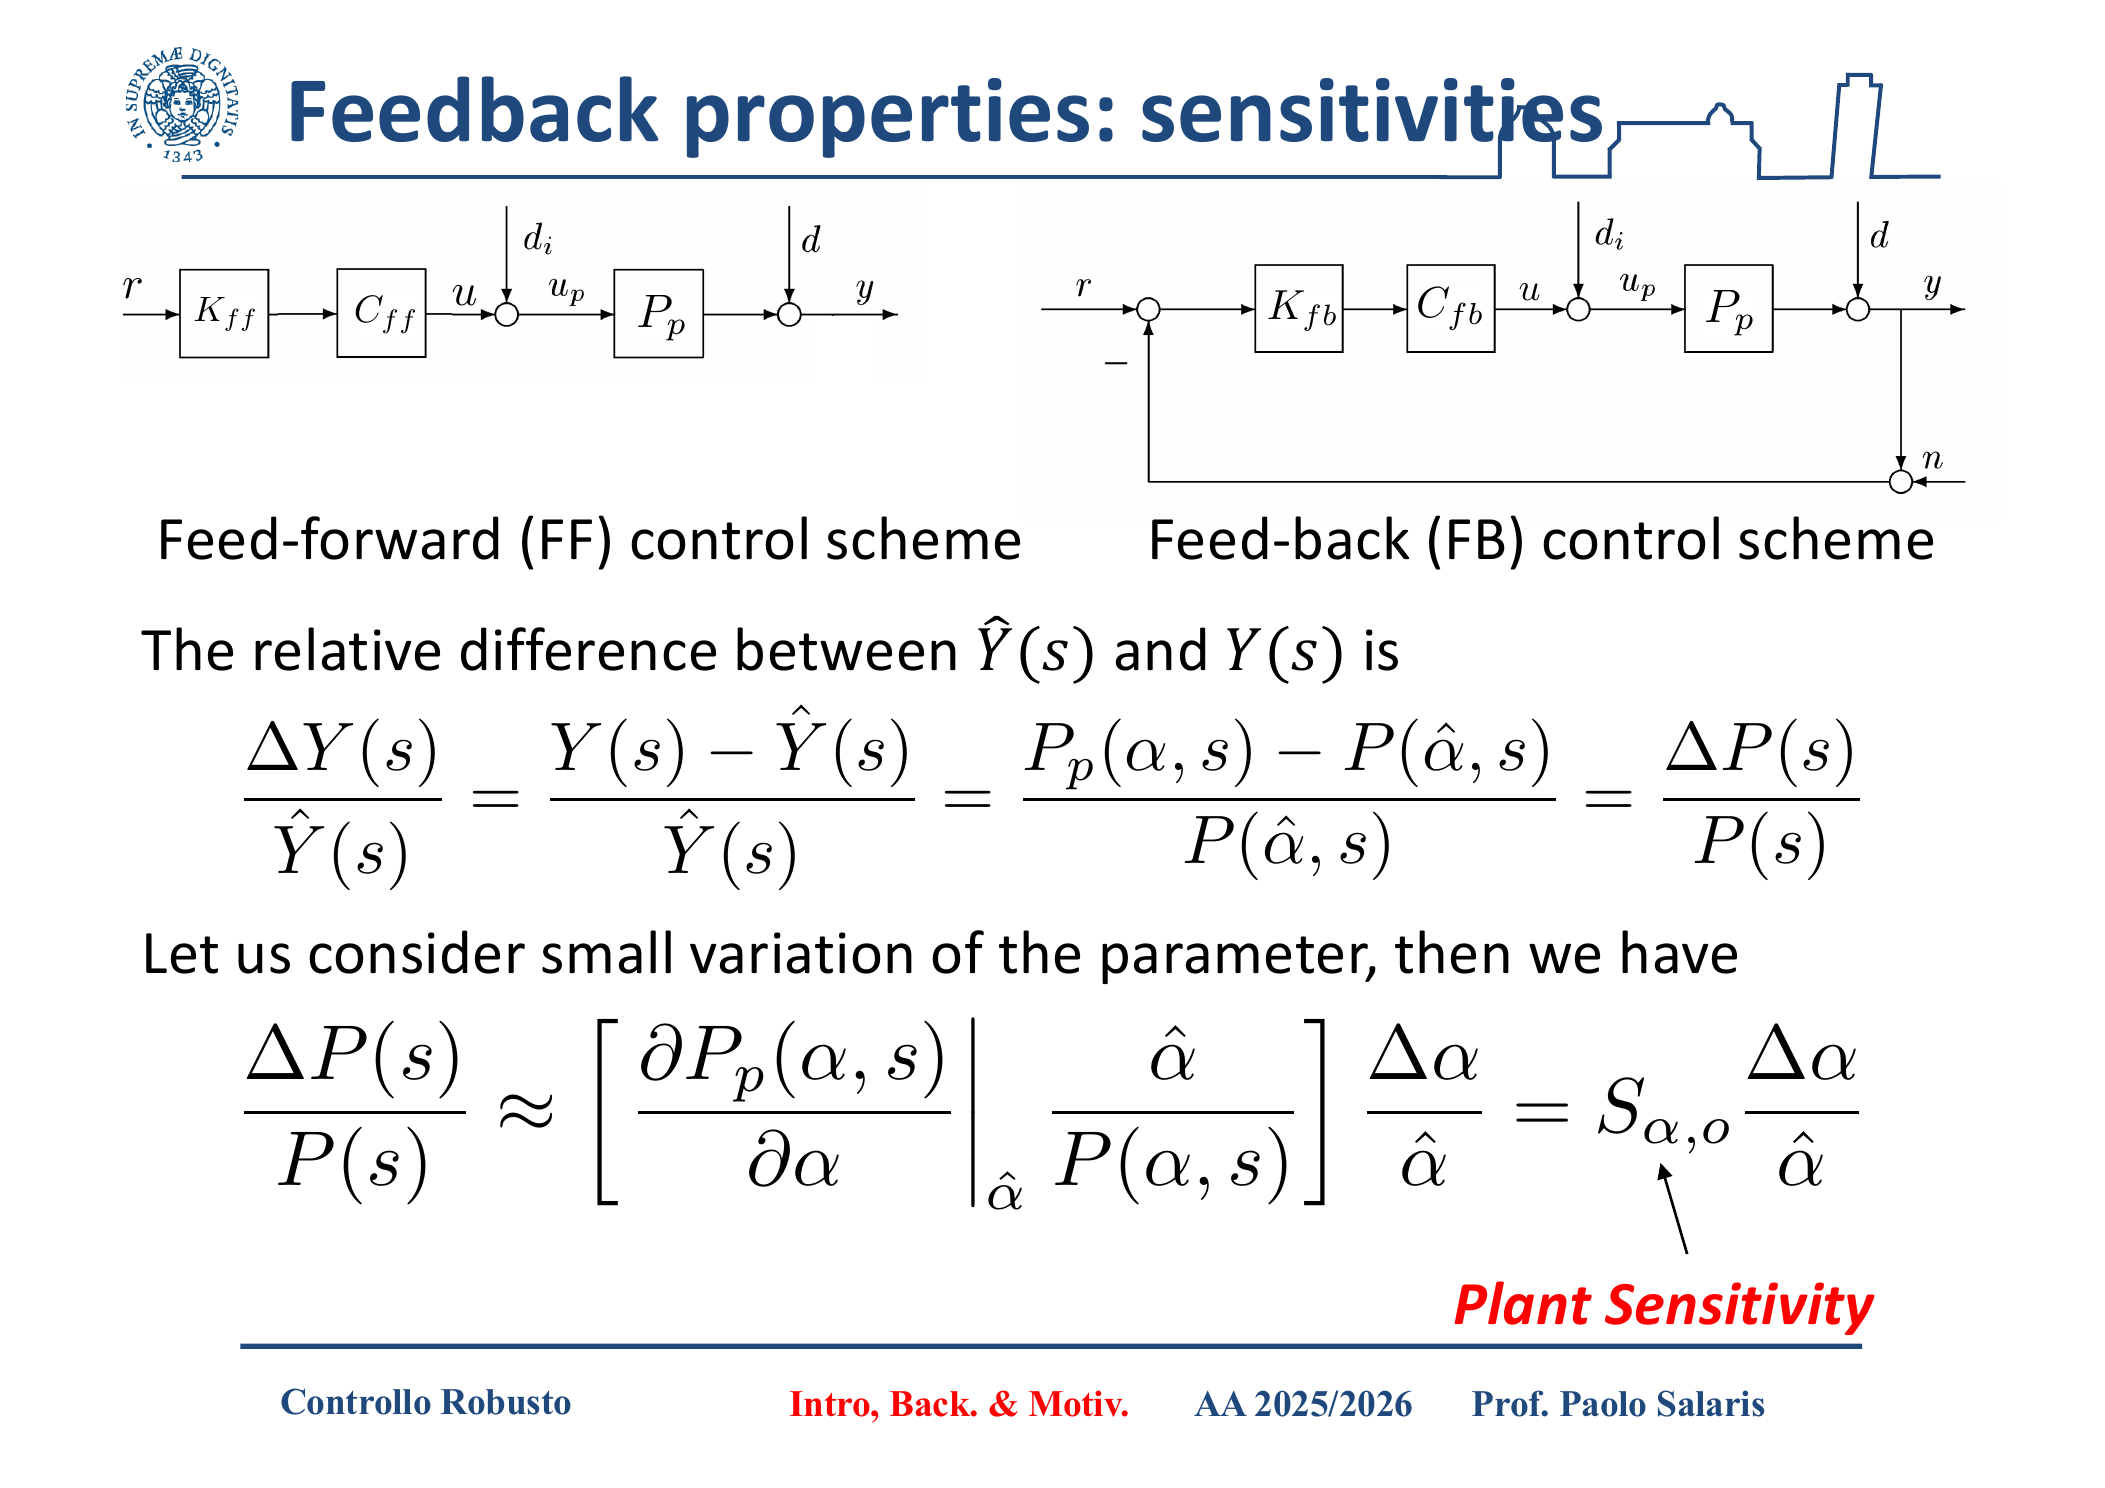
\includegraphics[width=0.82\textwidth]{images2/page-18.png}
    \caption{Definizione della sensitività dell'impianto tramite linearizzazione della perturbazione parametrica.}
\end{figure}

\subsubsection{Esempio elettromeccanico}

L'esempio delle slide considera un sistema del tipo
\begin{align*}
\tau \dot c(t)+c(t) &= Ku(t), \\
J\ddot\theta(t)+f\dot\theta(t) &= K_m c(t)+d(t),
\end{align*}
con stato
$$
x=\begin{bmatrix}\theta & \dot\theta & c\end{bmatrix}^T.
$$
Il modello in spazio di stato assume la forma
$$
\dot x=Ax+Bu, \qquad y=Cx,
$$
con matrici riportate esplicitamente in slide. Da qui si ricavano la funzione di trasferimento comando-uscita e quella disturbo-uscita:
$$
G_{ru}(s)=\frac{KK_m}{s(\tau s+1)(Js+f)}=P_p(s),
\qquad
G_{rd}(s)=\frac{1}{s(\tau s+1)}=D(s).
$$

Le slide mostrano poi due risultati notevoli:
$$
S_{K_m,o}=1,
\qquad
S_{\tau,o}=-\frac{\tau s}{\tau s+1}.
$$
Il primo dice che l'impianto dipende linearmente dal parametro $K_m$: una variazione relativa di $K_m$ produce la stessa variazione relativa nella funzione di trasferimento. Il secondo mostra invece una dipendenza frequenziale del contributo di $\tau$: a bassa frequenza l'effetto è piccolo, mentre ad alta frequenza tende in modulo a 1. Questo è un punto molto importante in robustezza, perché evidenzia che non tutte le incertezze pesano allo stesso modo in tutte le bande di frequenza.

\begin{figure}[H]
    \centering
    \begin{subfigure}{0.49\textwidth}
        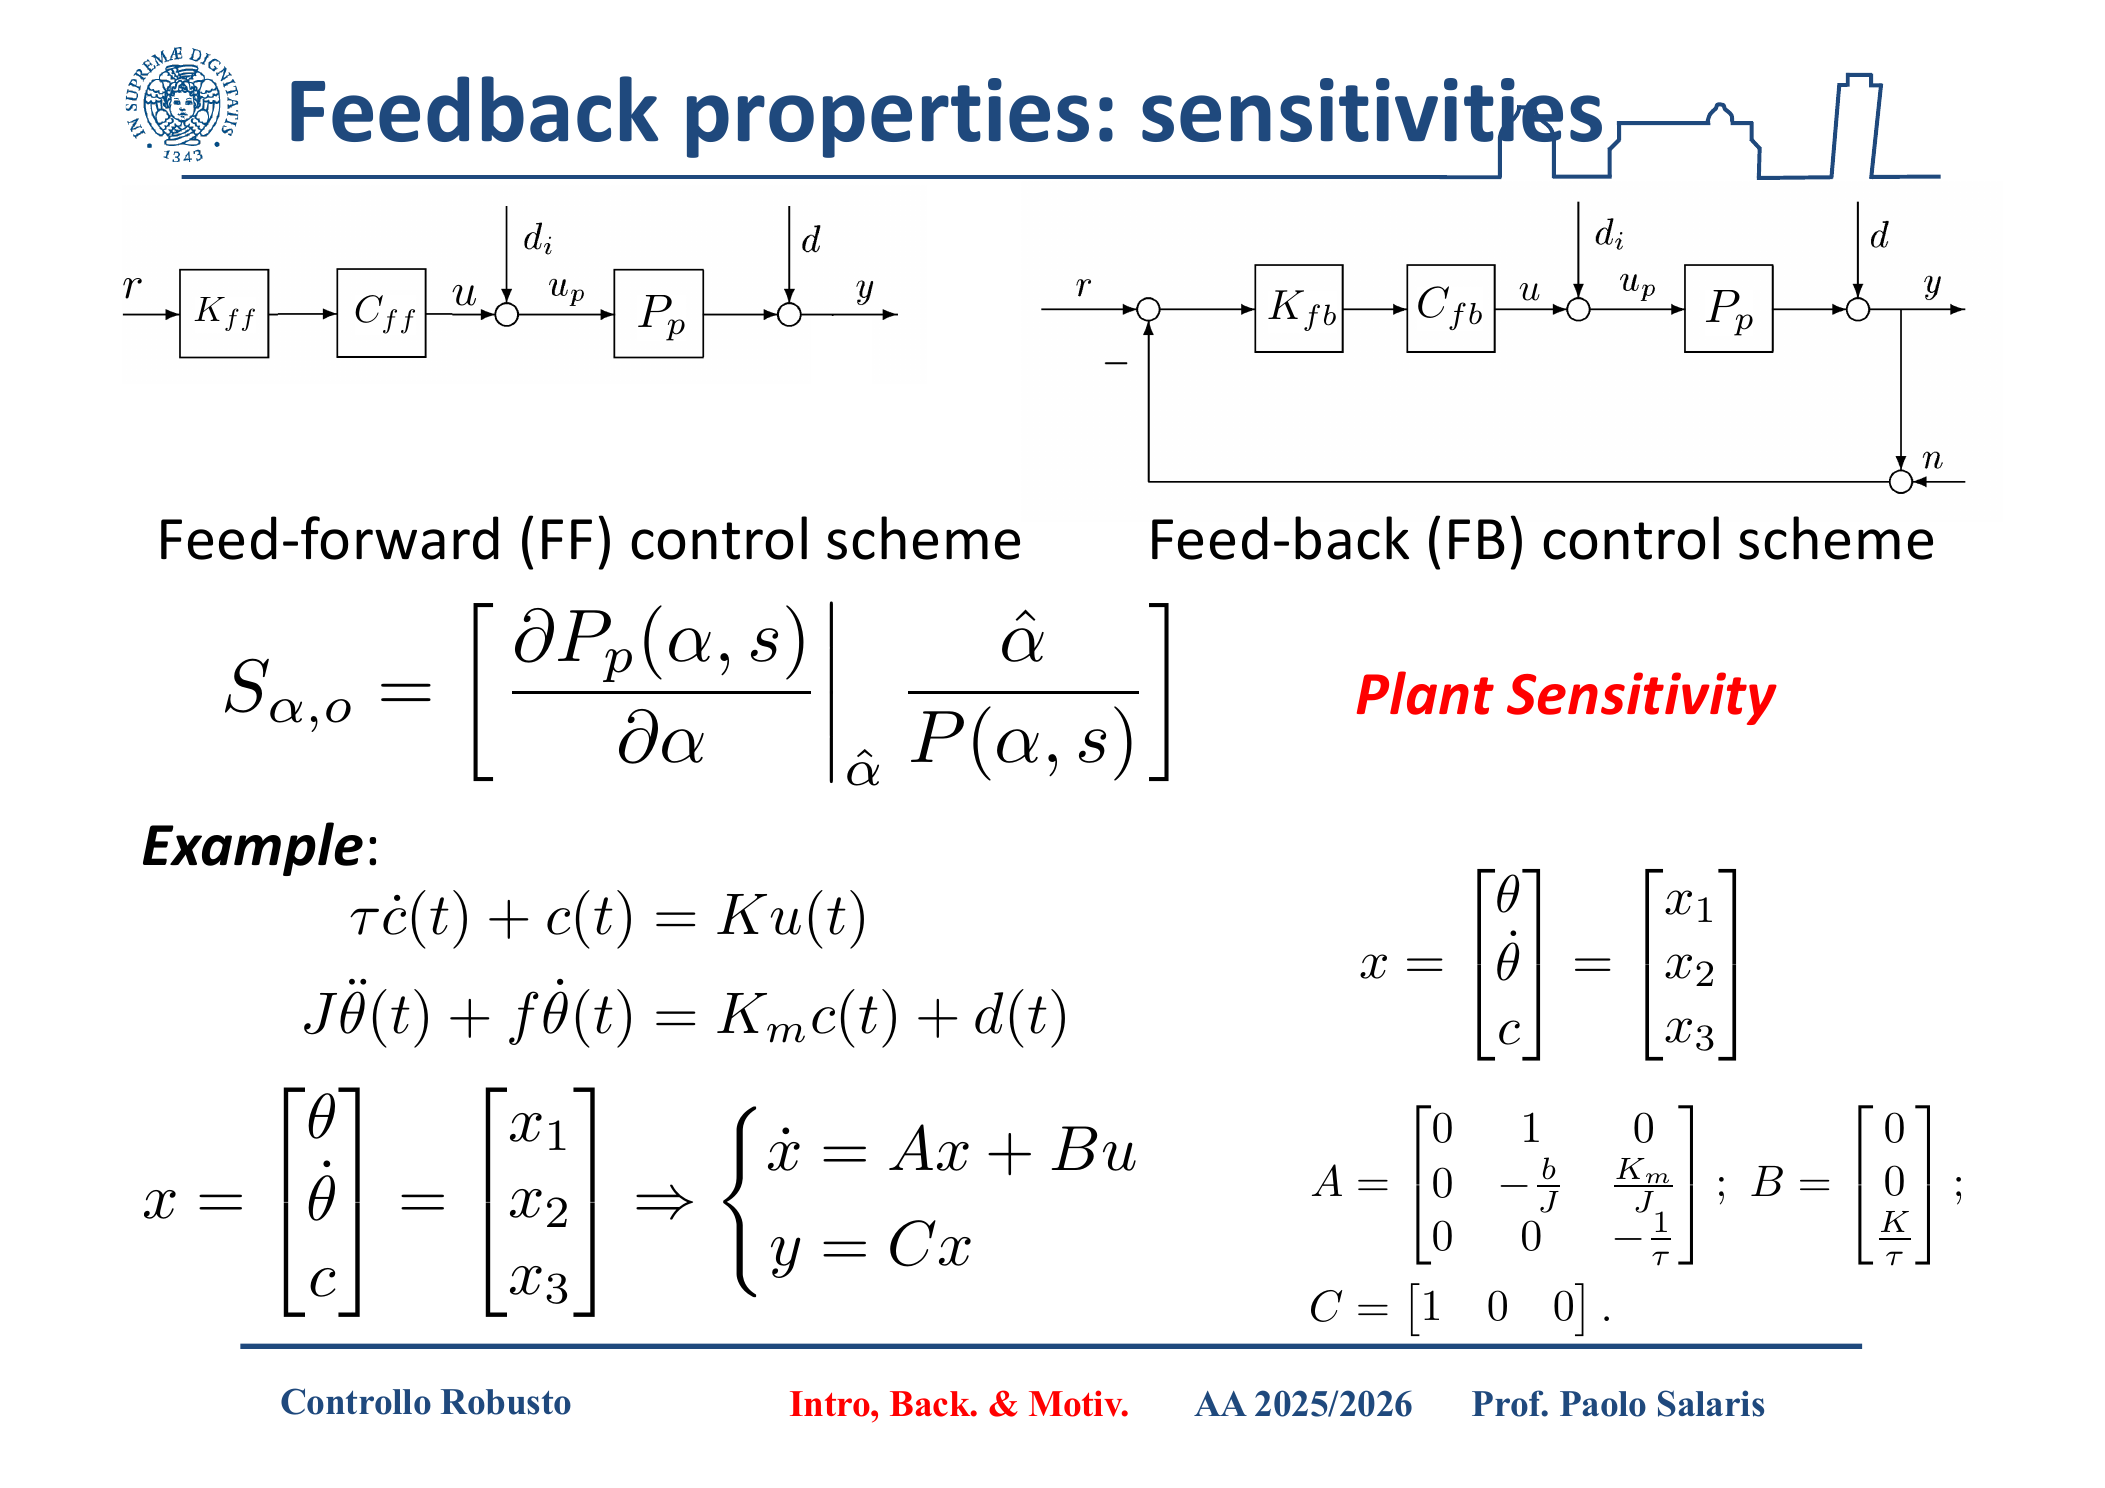
\includegraphics[width=\linewidth]{images2/page-19.png}
        \caption{Modello fisico e rappresentazione di stato.}
    \end{subfigure}
    \hfill
    \begin{subfigure}{0.49\textwidth}
        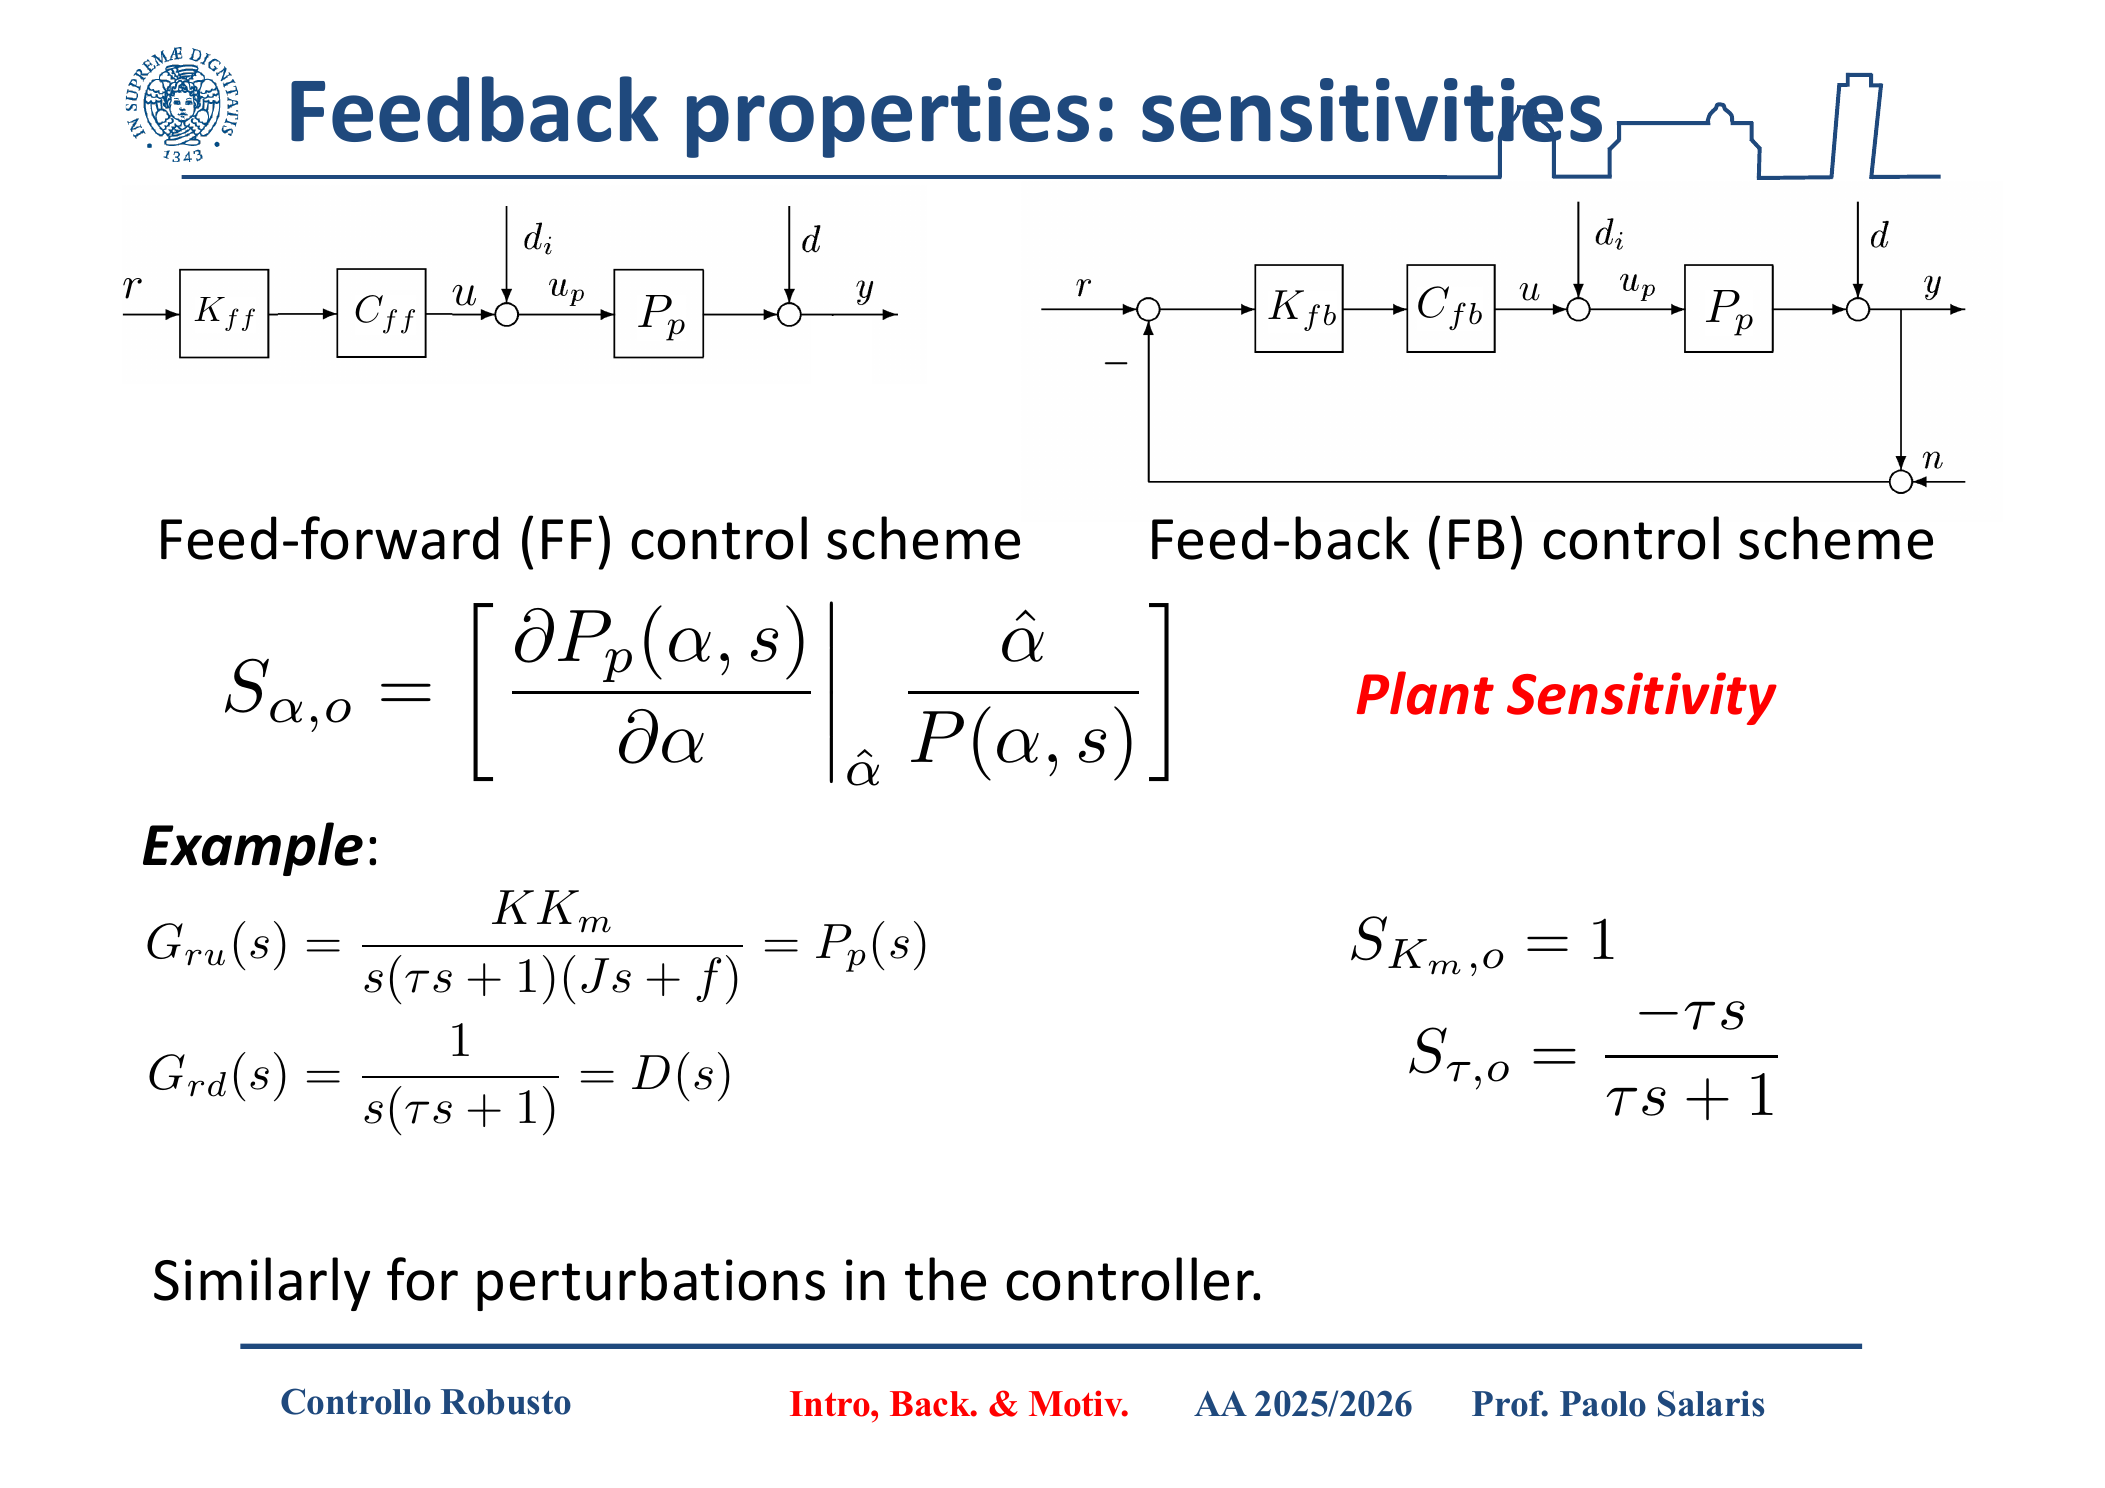
\includegraphics[width=\linewidth]{images2/page-20.png}
        \caption{Funzioni di trasferimento e sensitività parametriche.}
    \end{subfigure}
    \caption{Esempio di sensitività dell'impianto rispetto a parametri fisici del sistema.}
\end{figure}

\subsubsection{Dal feed-forward alla loop sensitivity}

Le ultime due slide spiegano perché la retroazione è utile per ridurre l'effetto delle incertezze. Nel caso feedback, con
$$
G_c(s)=\frac{K_{fb}C_{fb}(s)P_p(s)}{1+K_{fb}C_{fb}(s)P_p(s)},
$$
una piccola perturbazione dell'impianto induce una variazione relativa dell'uscita pari approssimativamente a
$$
\frac{\Delta Y(s)}{Y(s)}
=\frac{\Delta G_c(s)}{G_c(s)}
\approx
\frac{1}{1+K_{fb}C_{fb}(s)P_p(s)}\frac{\Delta P(s)}{P(s)}.
$$
Definendo la \emph{funzione di sensibilità del loop}
$$
S(s)=\frac{1}{1+L(s)}, \qquad L(s)=K_{fb}C_{fb}(s)P_p(s),
$$
si ottiene
$$
\frac{\Delta Y(s)}{Y(s)}
= S(s)S_{\alpha,o}(s)\frac{\Delta\alpha}{\hat\alpha}.
$$

Questa formula è uno dei risultati più importanti dell'intero capitolo. Dice che l'effetto dell'incertezza parametrica sull'uscita viene \emph{filtrato} dalla sensibilità $S(s)$. Dove il guadagno di anello è grande, $|L(s)|\gg1$, la sensibilità è piccola e il feedback attenua l'effetto dell'incertezza. Dove il guadagno di anello è piccolo, la riduzione scompare. In altre parole, la retroazione non elimina in assoluto la dipendenza dal modello, ma la redistribuisce in frequenza.

\begin{figure}[H]
    \centering
    \begin{subfigure}{0.49\textwidth}
        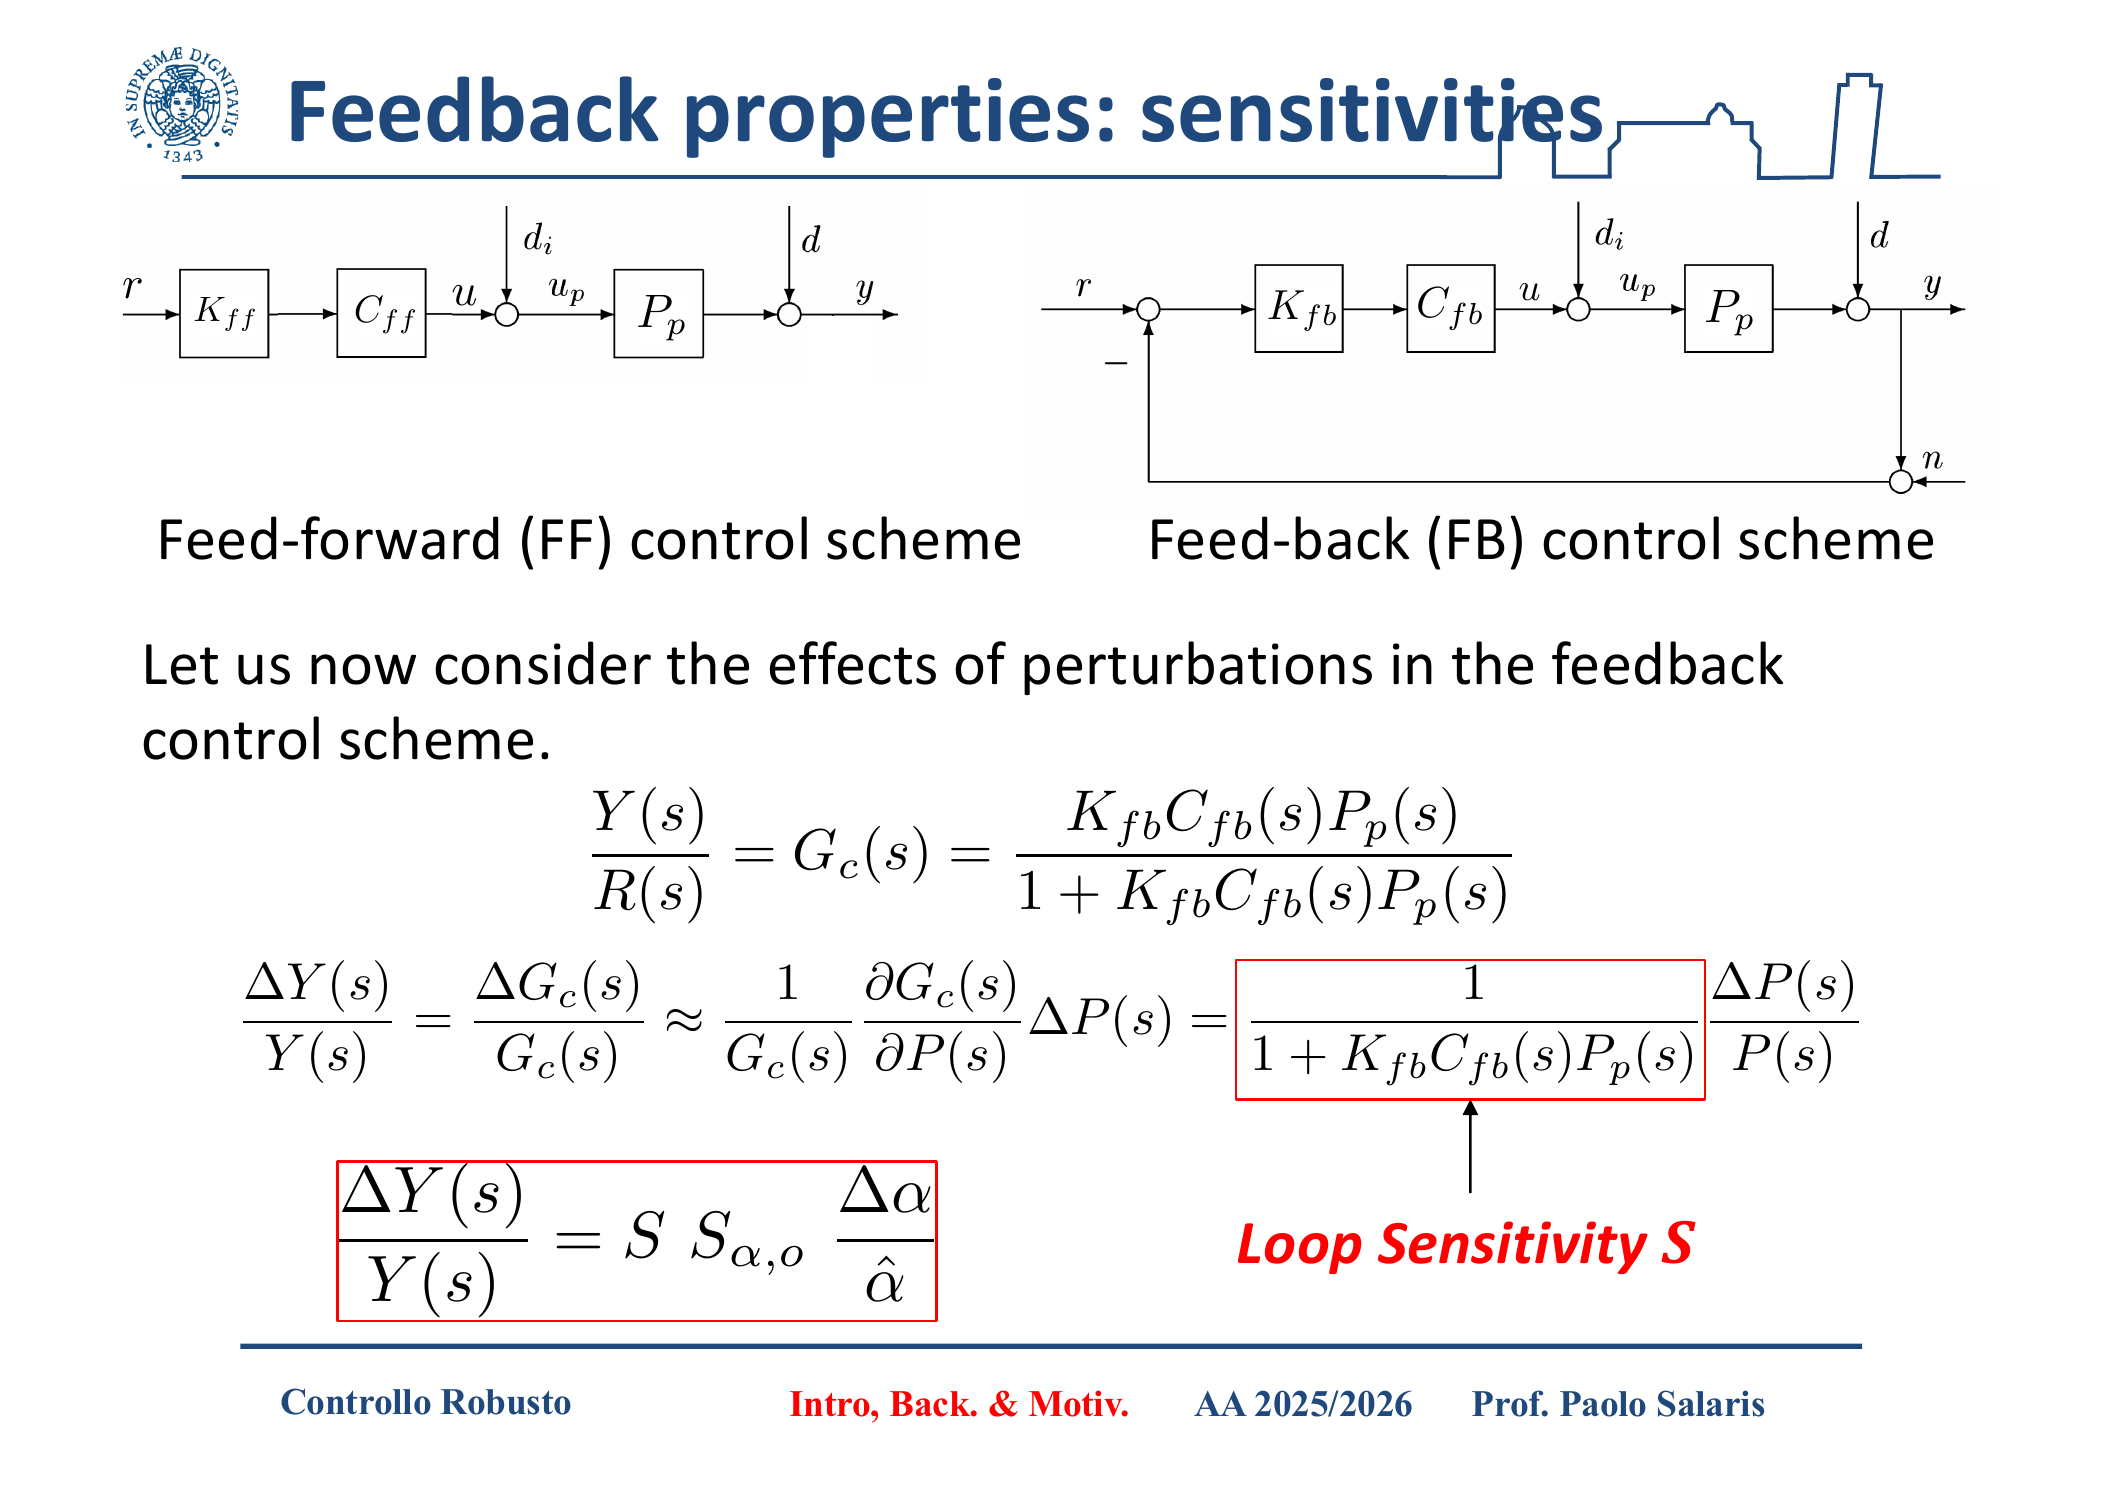
\includegraphics[width=\linewidth]{images2/page-21.png}
        \caption{Definizione della loop sensitivity $S(s)$.}
    \end{subfigure}
    \hfill
    \begin{subfigure}{0.49\textwidth}
        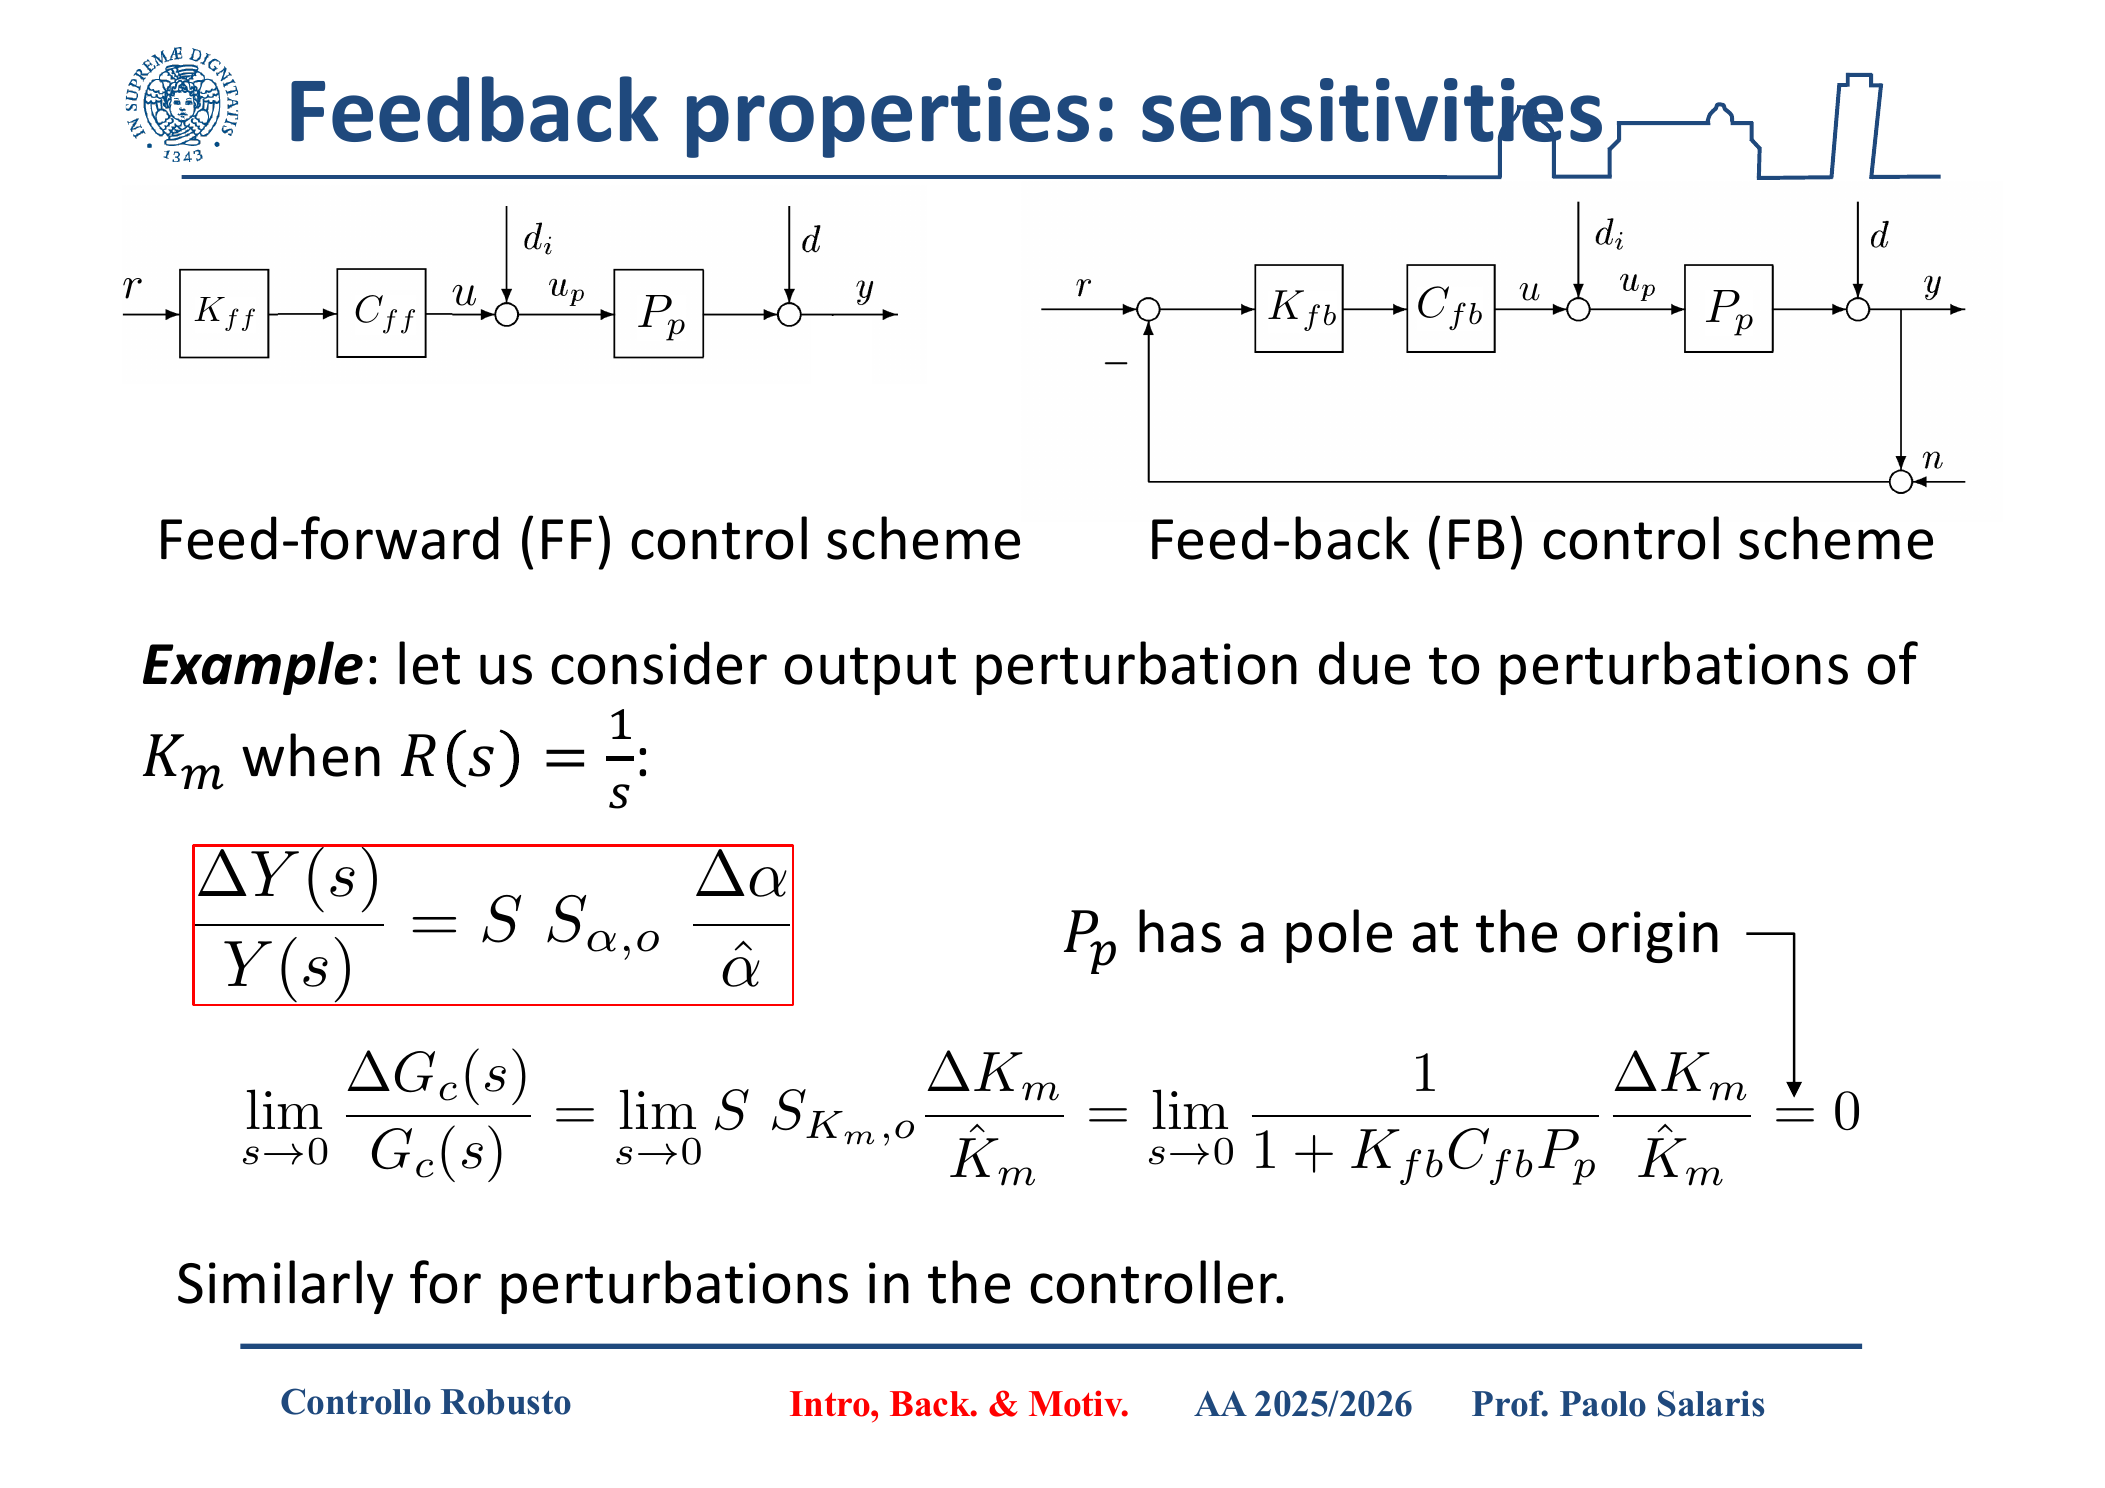
\includegraphics[width=\linewidth]{images2/page-22.png}
        \caption{Esempio a bassa frequenza con polo nell'origine.}
    \end{subfigure}
    \caption{La retroazione riduce l'effetto delle incertezze in misura proporzionale a $S(s)=1/(1+L(s))$.}
\end{figure}

\subsubsection{Interpretazione fisica della funzione di sensibilità}

La funzione
$$
S(s)=\frac{1}{1+L(s)}
$$
ha un significato molto ampio. Non misura solo la sensitività alle variazioni dell'impianto. Essa quantifica anche:
\begin{itemize}
    \item la sensibilità del chiuso a perturbazioni parametriche del loop;
    \item il rigetto dei disturbi in certe configurazioni di iniezione;
    \item il grado con cui l'errore viene forzato verso zero nelle bande dove il loop gain è elevato.
\end{itemize}

Se l'impianto possiede un polo nell'origine, allora a bassa frequenza $L(s)$ cresce e $S(0)=0$, o almeno tende a zero nei casi ideali. Questo spiega il risultato dell'ultima slide: per perturbazioni sul parametro $K_m$ e riferimento a gradino, l'effetto relativo sull'uscita tende a zero quando $s\to0$. La presenza dell'integratore nel loop rende il sistema insensibile a quel tipo di incertezza nel regime stazionario.

Questo è un esempio concreto del vantaggio della retroazione rispetto al feed-forward. Nel feed-forward l'errore di modello passa direttamente all'uscita. Nel feedback l'errore viene attenuato da un meccanismo correttivo che confronta continuamente uscita e riferimento.

\begin{keybox}
La robustezza non è una proprietà assoluta ma frequenziale. La retroazione attenua l'effetto delle incertezze dove il guadagno di anello è alto, cioè dove $S(s)$ è piccolo. Lo paga però in altre bande tramite i noti compromessi fra sensibilità, rumore e margini di stabilità.
\end{keybox}

\subsection{Sintesi finale}

Il capitolo mette insieme tre idee che in controllo robusto non vanno mai separate.

La prima è che la nozione corretta di stabilità di una struttura in retroazione è la \emph{stabilità interna}. Non basta controllare l'equazione caratteristica ridotta e non bastano cancellazioni formali di poli e zeri. Tutte le mappe interne devono essere proprie e stabili.

La seconda è che le \emph{specifiche statiche e dinamiche} hanno una traduzione strutturale e frequenziale precisa. Le prestazioni statiche dipendono dal tipo del sistema e dal principio del modello interno. Le prestazioni dinamiche sono legate a banda passante, frequenza di attraversamento e margine di fase.

La terza è che la \emph{sensitività} fornisce il ponte diretto fra prestazione nominale e robustezza rispetto alle incertezze di modello. La funzione di sensibilità $S(s)=1/(1+L(s))$ è l'oggetto che quantifica quanto il feedback riesca a proteggere il comportamento del sistema dai cambiamenti parametrici.

In sintesi, il quadro concettuale è il seguente: prima si garantisce che l'interconnessione sia ben posta e internamente stabile; poi si progetta per ottenere l'errore a regime richiesto e un transitorio accettabile; infine si verifica che tali prestazioni rimangano ragionevolmente insensibili alle incertezze realistiche del modello.

\clearpage
\phantomsection
\section*{Appendice}
\addcontentsline{toc}{section}{Appendice}

\subsection*{Nota sulle convenzioni di segno}
\phantomsection
\addcontentsline{toc}{subsection}{Nota sulle convenzioni di segno}

In letteratura esistono convenzioni diverse per definire il numero di avvolgimenti: alcuni autori contano gli avvolgimenti orari come positivi, altri quelli antiorari; alcuni lavorano con il contorno di Nyquist nel semipiano destro percorso in senso orario, altri incorporano il segno direttamente nelle formule finali. Per questo motivo possono comparire versioni del criterio scritte come
$$
N = Z - P
\qquad \text{oppure} \qquad
N = P - Z.
$$

Non c’è contraddizione. Ciò che conta è mantenere coerente, dall’inizio alla fine, il verso del contorno, il segno della variazione di argomento e il verso con cui si contano gli avvolgimenti del punto critico.

\subsection*{Riferimento al materiale originale}
\phantomsection
\addcontentsline{toc}{subsection}{Riferimento al materiale originale}

Questo elaborato è una traduzione e rielaborazione estesa del PDF delle slide ``Controllo Robusto Intro, Back.\ \& Motiv. AA 2025/2026'' del Prof.\ Paolo Salaris, caricato dall’utente come materiale di partenza.


\newpage

\section{Lezione 4}

\subsection{Visione d'insieme della lezione}

Questa lezione occupa una posizione di snodo molto chiara all'interno del capitolo. La Lezione 3 aveva introdotto tre idee fondamentali: la stabilità interna come nozione corretta di stabilità del ciclo chiuso, il legame fra specifiche statiche e dinamiche da un lato e frequenza di attraversamento o margine di fase dall'altro, e infine la comparsa della funzione di sensibilità
$$
S(s)=\frac{1}{1+L(s)}
$$
come fattore che attenua l'effetto delle incertezze parametriche sul comportamento chiuso. La Lezione 4 prende proprio quest'ultimo oggetto e lo porta al centro della scena: non più semplice formula finale di un esempio, ma vero linguaggio con cui leggere robustezza, prestazioni e limiti del feedback.

Il primo passo consiste nel chiarire, nel caso SISO, come \emph{return difference}, sensibilità $S$ e sensibilità complementare $T$ organizzino in modo unitario i problemi di tracking, rigetto dei disturbi, trasmissione del rumore di misura e scelta della banda passante. Il secondo passo è l'estensione al caso MIMO: qui le stesse idee sopravvivono, ma diventano matriciali e soprattutto \emph{direzionali}. Non basta più chiedersi se il guadagno sia grande o piccolo: bisogna capire in quali combinazioni di ingressi e uscite esso lo sia.

Per questo motivo l'ultima parte della lezione, dedicata a norme, valori singolari e SVD, non è un'appendice matematica scollegata dal resto. È il ponte naturale verso la Lezione 5. Lì infatti le matrici di sensitività introdotte qui verranno trasformate in vere condizioni di progetto, espresse in termini di guadagni principali e di \emph{loop shaping}. In breve: la Lezione 3 dice \emph{perché} compare $S$; la Lezione 4 spiega \emph{che cosa misura} $S$ e come si generalizza; la Lezione 5 userà queste quantità per dire \emph{come si progetta}.

\begin{keybox}
La Lezione 4 è la cerniera del capitolo. Dalla Lezione 3 eredita la domanda ``quanto il chiuso resta sensibile a modello, disturbi e limiti dinamici?''; alla Lezione 5 consegna la risposta operativa: tali richieste vanno lette e modellate attraverso $S$, $T$, le loro versioni matriciali e i valori singolari.
\end{keybox}

\begin{focusbox}
\textbf{Idea guida della lezione.} Il feedback non viene giudicato soltanto dalla stabilità del sistema chiuso, ma da \emph{quanto} il sistema rimane sensibile a errori di modello, disturbi, rumore e diverse direzioni di eccitazione. Il linguaggio naturale per esprimere questo fatto è quello di $S$, $T$ e, nel caso MIMO, dei valori singolari. In questo senso la lezione costruisce davvero la grammatica concettuale che la Lezione 5 userà poi per formulare regole di progetto.
\end{focusbox}

\subsection{Feedback, incertezza di modello e return difference}

Le prime slide riprendono in forma più sistematica il confronto fra feed-forward e feedback già emerso alla fine della Lezione 3. Nel caso feed-forward l’azione di controllo viene calcolata una volta per tutte sul modello nominale del processo. Se il processo reale differisce da quel modello, l’errore passa direttamente all’uscita: la struttura non possiede alcun meccanismo interno di correzione.

Nel caso feedback, invece, l’uscita viene continuamente confrontata con il comportamento desiderato e il comando viene aggiornato in tempo reale. Per piccole variazioni di modello, questa differenza si traduce in una relazione molto importante:
$$
\frac{\Delta Y(s)}{Y(s)} \approx S(s)\,\frac{\Delta P(s)}{P(s)}.
$$
Il messaggio è semplice ma decisivo: la retroazione è utile non perché elimini l’incertezza del modello, ma perché ne \emph{filtra} l’effetto attraverso la funzione di sensibilità. Dove $|S(j\omega)|<1$, il feedback rende il sistema meno vulnerabile del corrispondente schema feed-forward.

Lo stesso fatto può essere espresso introducendo la \emph{return difference}. Nella convenzione standard di retroazione negativa adottata nel resto del testo si pone
$$
F(s)=1+L(s),
\qquad
S(s)=\frac{1}{F(s)},
\qquad
T(s)=\frac{L(s)}{F(s)}.
$$
Nelle slide compare talvolta la scrittura $1-L(s)$: non c’è contraddizione, è solo una diversa convenzione di segno incorporata nella definizione del loop transfer. La sostanza non cambia: la return difference coincide con il denominatore del ciclo chiuso e misura quanto il sistema sia lontano dalla condizione critica in cui tale denominatore si annulla.

L’interpretazione geometrica è altrettanto importante. Nel piano di Nyquist, il modulo di $F(j\omega)$ rappresenta la distanza del luogo d’anello dal punto critico. Se questa distanza si riduce troppo, allora $S(j\omega)$ cresce, il sistema diventa fragile e piccole variazioni del modello possono produrre grandi variazioni delle mappe chiuse o perfino perdita di stabilità. La return difference è quindi un primo indicatore diretto di robustezza: non dice ancora \emph{come} progettare il loop, ma dice già \emph{quanto} esso sia vicino a una situazione pericolosa.

\begin{figure}[H]
    \centering
    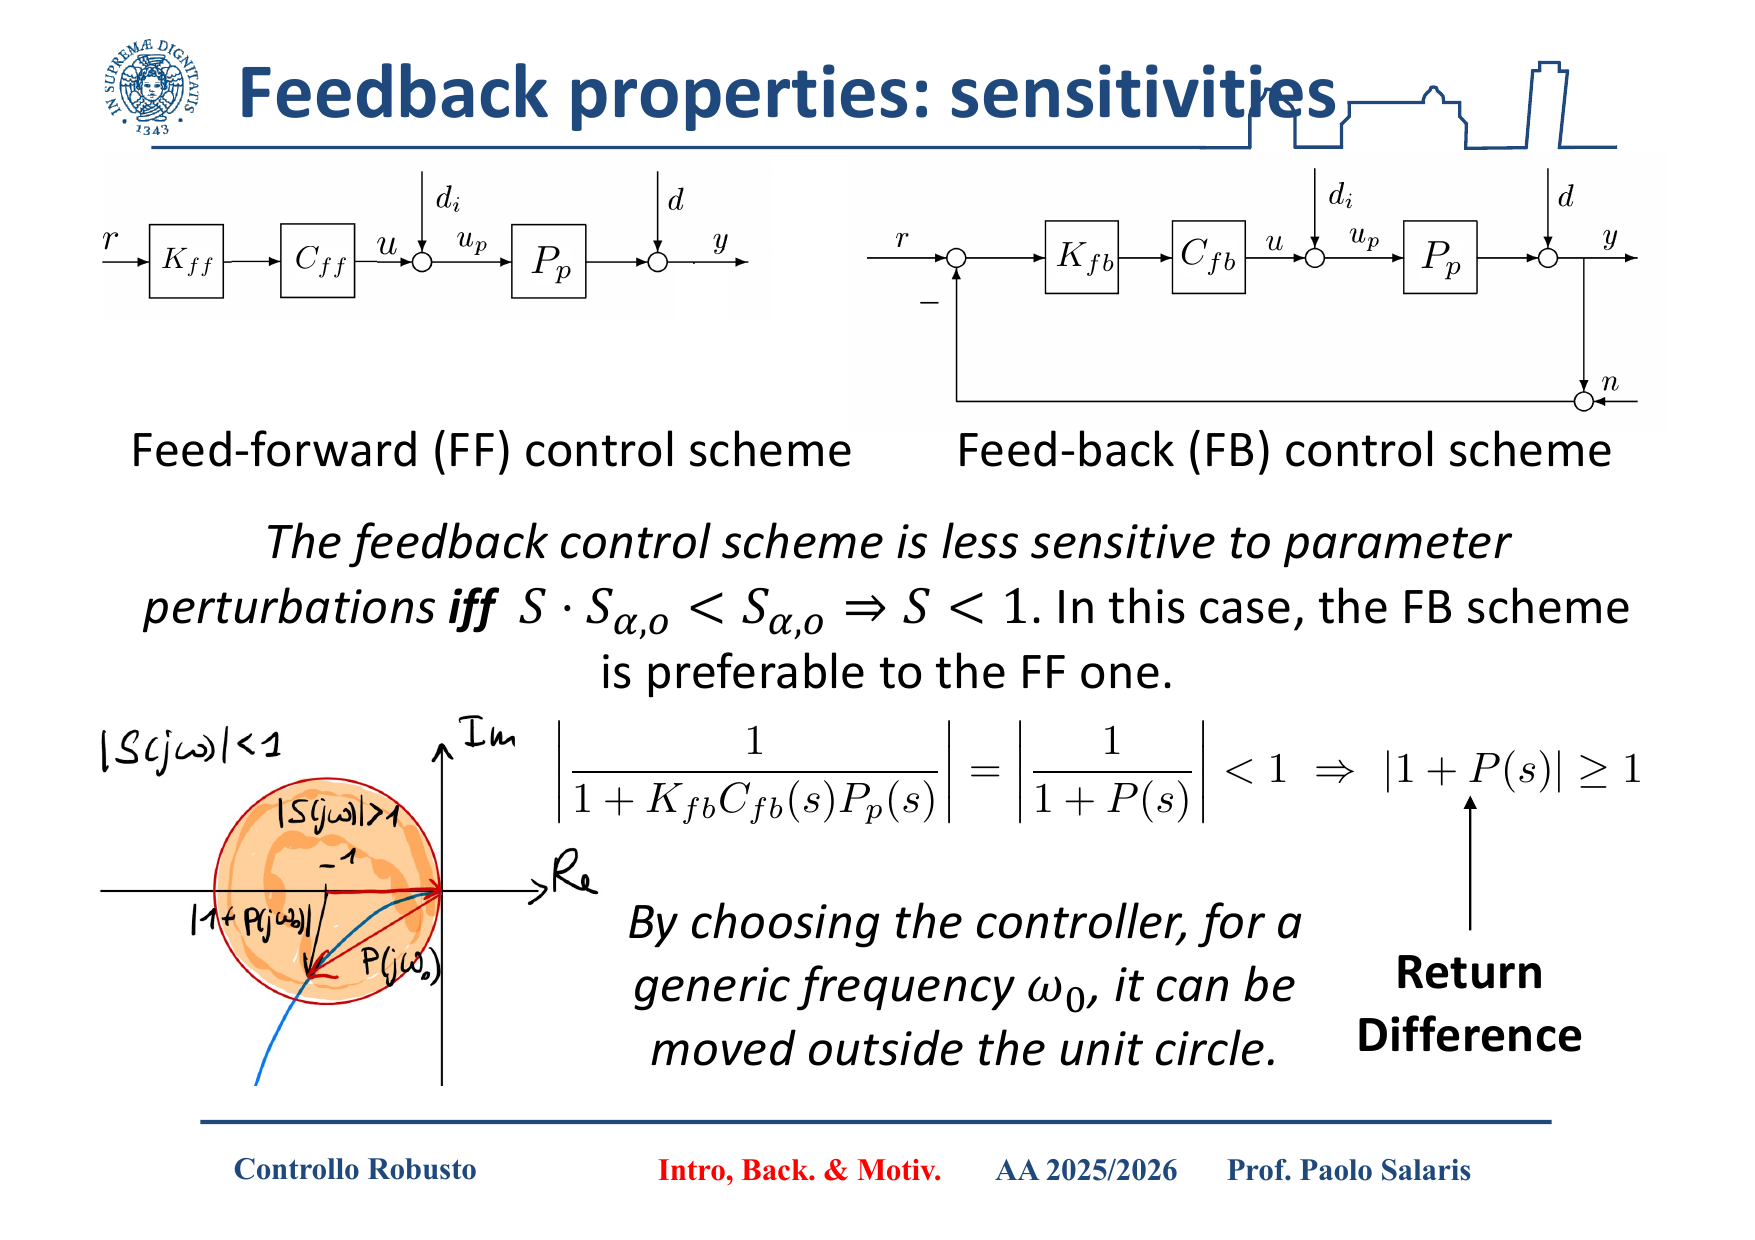
\includegraphics[width=0.82\textwidth]{images3/slide-01.png}
    \caption{Confronto tra struttura feed-forward e struttura feedback in presenza di perturbazioni parametriche del processo.}
\end{figure}

\begin{figure}[H]
    \centering
    \begin{subfigure}{0.48\textwidth}
        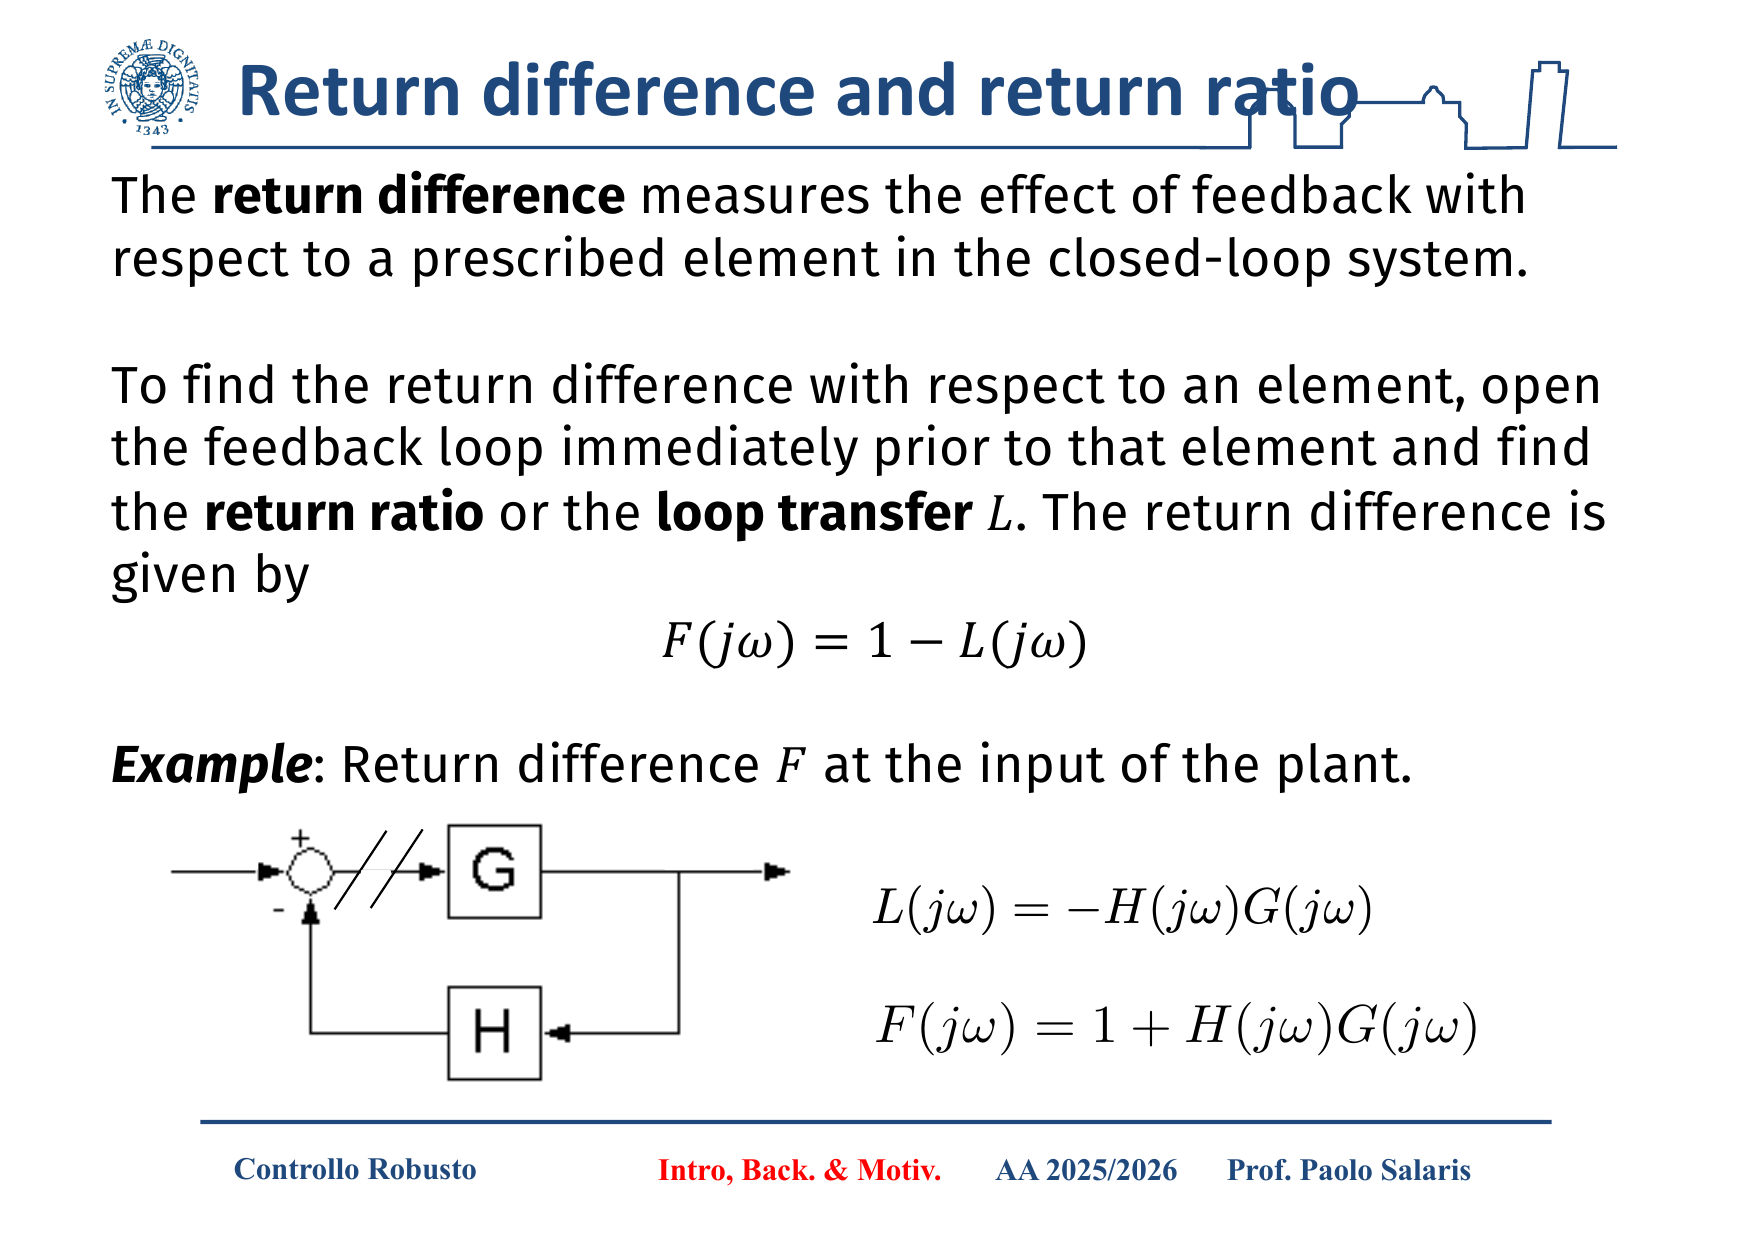
\includegraphics[width=\linewidth]{images3/slide-02.png}
        \caption{La return difference si ottiene aprendo l’anello nel punto desiderato e calcolando il ritorno complessivo.}
    \end{subfigure}
    \hfill
    \begin{subfigure}{0.48\textwidth}
        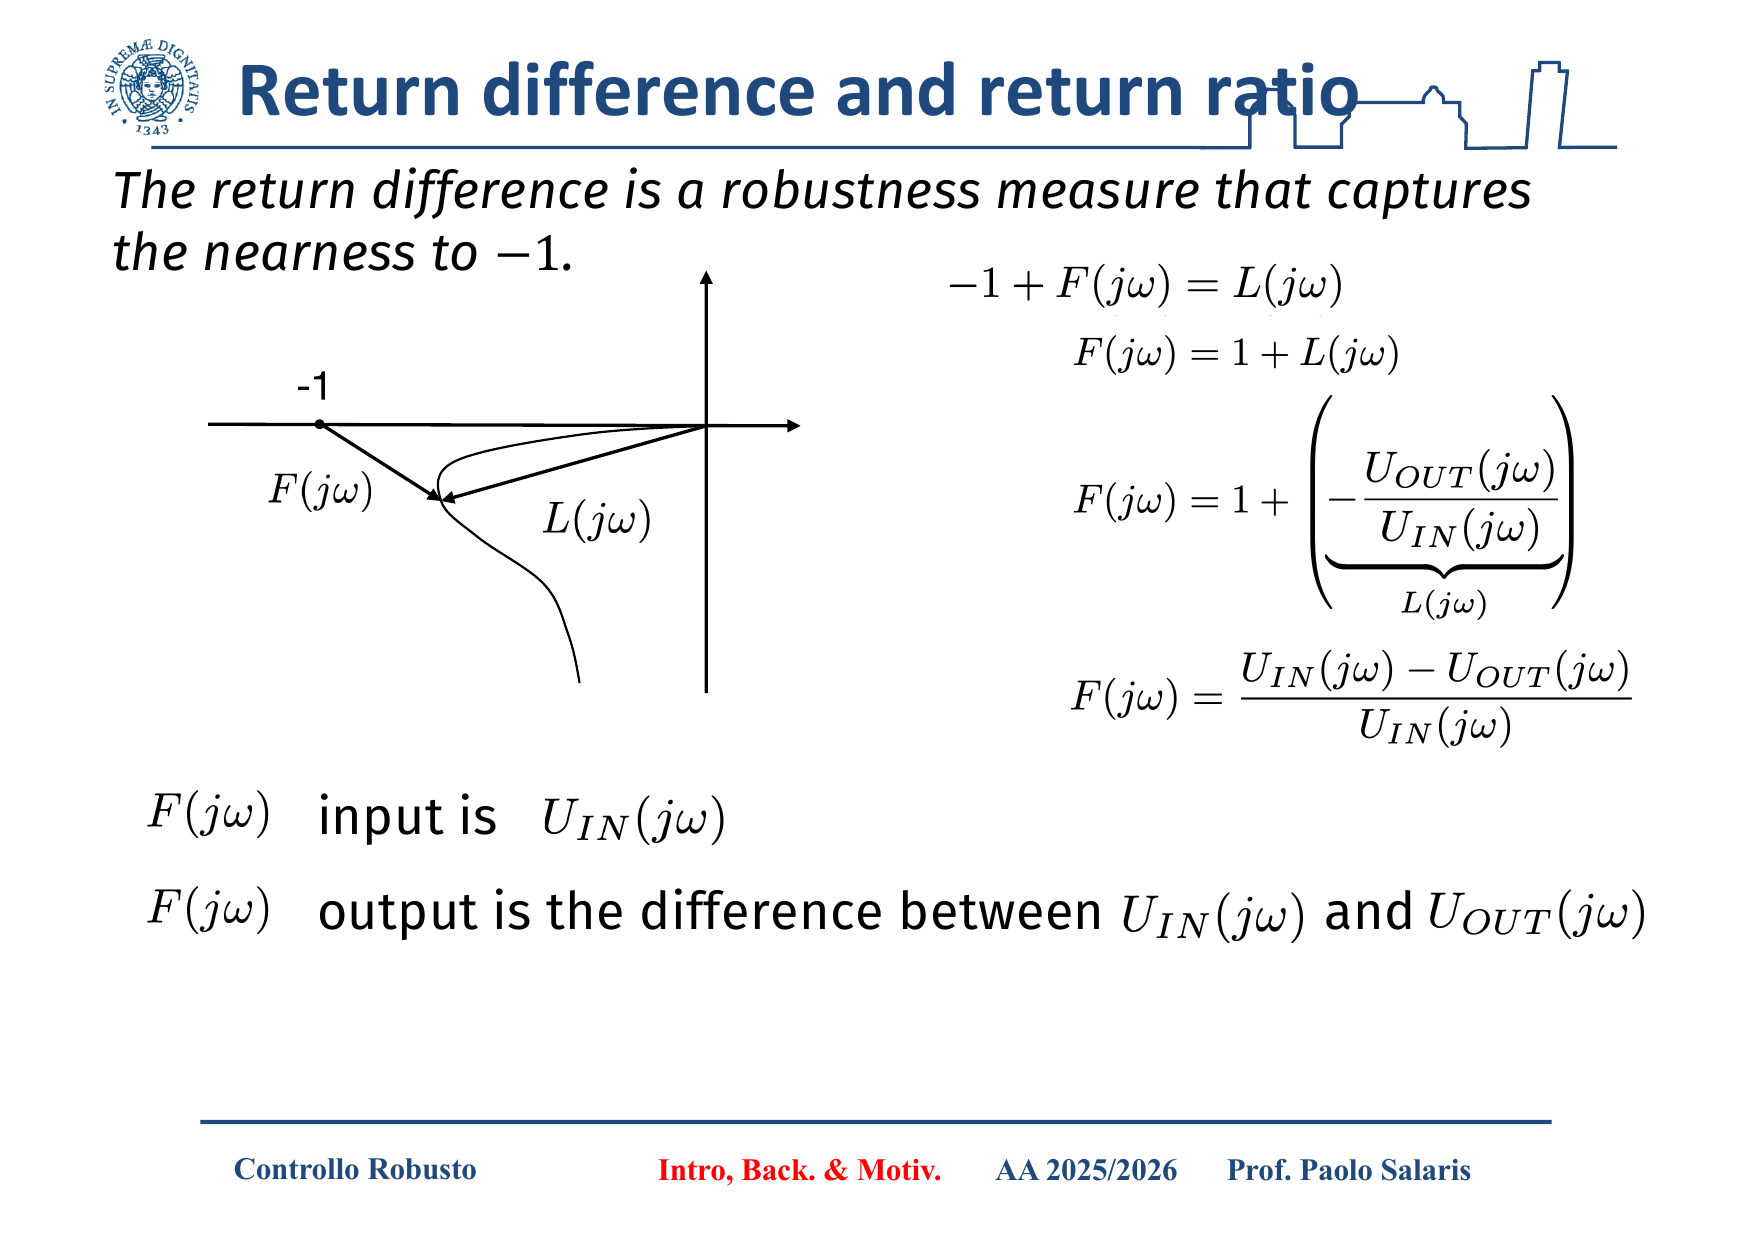
\includegraphics[width=\linewidth]{images3/slide-03.png}
        \caption{La distanza dal punto critico fornisce una misura diretta della fragilità del ciclo chiuso.}
    \end{subfigure}
    \caption{Le prime slide mostrano che il vantaggio del feedback si legge già nel denominatore dell’anello chiuso.}
\end{figure}

\subsection{Sensitività, disturbi, rumore e banda passante}

Una volta introdotte return difference e return ratio, la lezione passa al loro significato operativo. La quarta slide considera perturbazioni nel ramo di misura, cioè imperfezioni del sensore. In questo caso compare in modo naturale la \emph{sensibilità complementare}
$$
T(s)=\frac{L(s)}{1+L(s)},
\qquad
S(s)=\frac{1}{1+L(s)},
\qquad
S(s)+T(s)=1.
$$
La relazione $S+T=1$ è molto più di una semplice identità algebrica: esprime il vincolo strutturale che governa tutto il progetto robusto classico. Se in una certa banda di frequenza si rende molto piccolo $S$, allora in quella stessa banda $T$ deve avvicinarsi a $1$; se si vuole rendere piccolo $T$, allora è inevitabile lasciare crescere $S$.

Questo primo trade-off diventa chiarissimo non appena si guardano i canali chiusi di riferimento, disturbo e rumore. Assumendo per semplicità $H(s)=1$, l’uscita può essere scritta nella forma
$$
y = T(r-n) + S\,d + S\,P\,d_i.
$$
Il riferimento $r$ e il rumore di misura $n$ attraversano quindi $T$, mentre i disturbi applicati direttamente all’uscita del processo o prima del processo vengono filtrati da $S$ oppure da $SP$. In poche righe si riassumono così tre obiettivi distinti del progetto:
\begin{itemize}
    \item buon tracking del riferimento;
    \item buon rigetto dei disturbi sul processo;
    \item scarsa trasmissione del rumore di misura.
\end{itemize}

Nel dominio della frequenza questi obiettivi si traducono in richieste molto precise. Alle basse frequenze si desidera
$$
T(j\omega)\approx 1,
\qquad
S(j\omega)\approx 0,
$$
per seguire bene il riferimento e rigettare i disturbi lenti. Alle alte frequenze, invece, si vuole
$$
T(j\omega)\approx 0,
\qquad
S(j\omega)\approx 1,
$$
così che il rumore di misura non venga trasmesso all’uscita e il loop non continui a inseguire dinamiche per cui il modello non è più affidabile.

Qui si vede molto bene il collegamento con la Lezione 3. Là banda passante, rapidità del transitorio ed errore a regime erano stati introdotti come specifiche statiche e dinamiche; qui le stesse richieste vengono riscritte direttamente in termini di sensitività. Dire che un sistema deve essere rapido e accurato a bassa frequenza equivale a chiedere che il suo $T$ si comporti come un passa-basso unitario nella banda utile, mentre dire che il sistema deve restare robusto e poco sensibile al rumore equivale a imporre il decadimento di $T$ alle frequenze elevate.

La nozione di \emph{banda passante} nasce proprio da questa lettura. In prima approssimazione si identifica la banda del chiuso come l’intervallo di frequenze in cui $|T(j\omega)|$ resta vicino a $1$, con frequenza di taglio individuata dalla soglia di \SI{-3}{dB}:
$$
|T(j\omega_B)|=\frac{1}{\sqrt{2}}.
$$
Una banda più ampia tende a corrispondere a un sistema più rapido, ma rende anche più difficile attenuare rumore e incertezza alle alte frequenze. Questo è il motivo per cui la banda passante non può essere scelta guardando solo la rapidità: è già una scelta di compromesso tra prestazione nominale e robustezza.

\begin{keybox}
La lezione rende esplicita una regola che in forma embrionale era già presente nella Lezione 3: non esiste un feedback che renda contemporaneamente piccoli $S$ e $T$ a tutte le frequenze. Il progetto consiste nel distribuire il compromesso nel modo corretto, lasciando $T$ alto dove servono prestazioni e imponendone il decadimento dove dominano rumore e incertezza.
\end{keybox}

\begin{figure}[H]
    \centering
    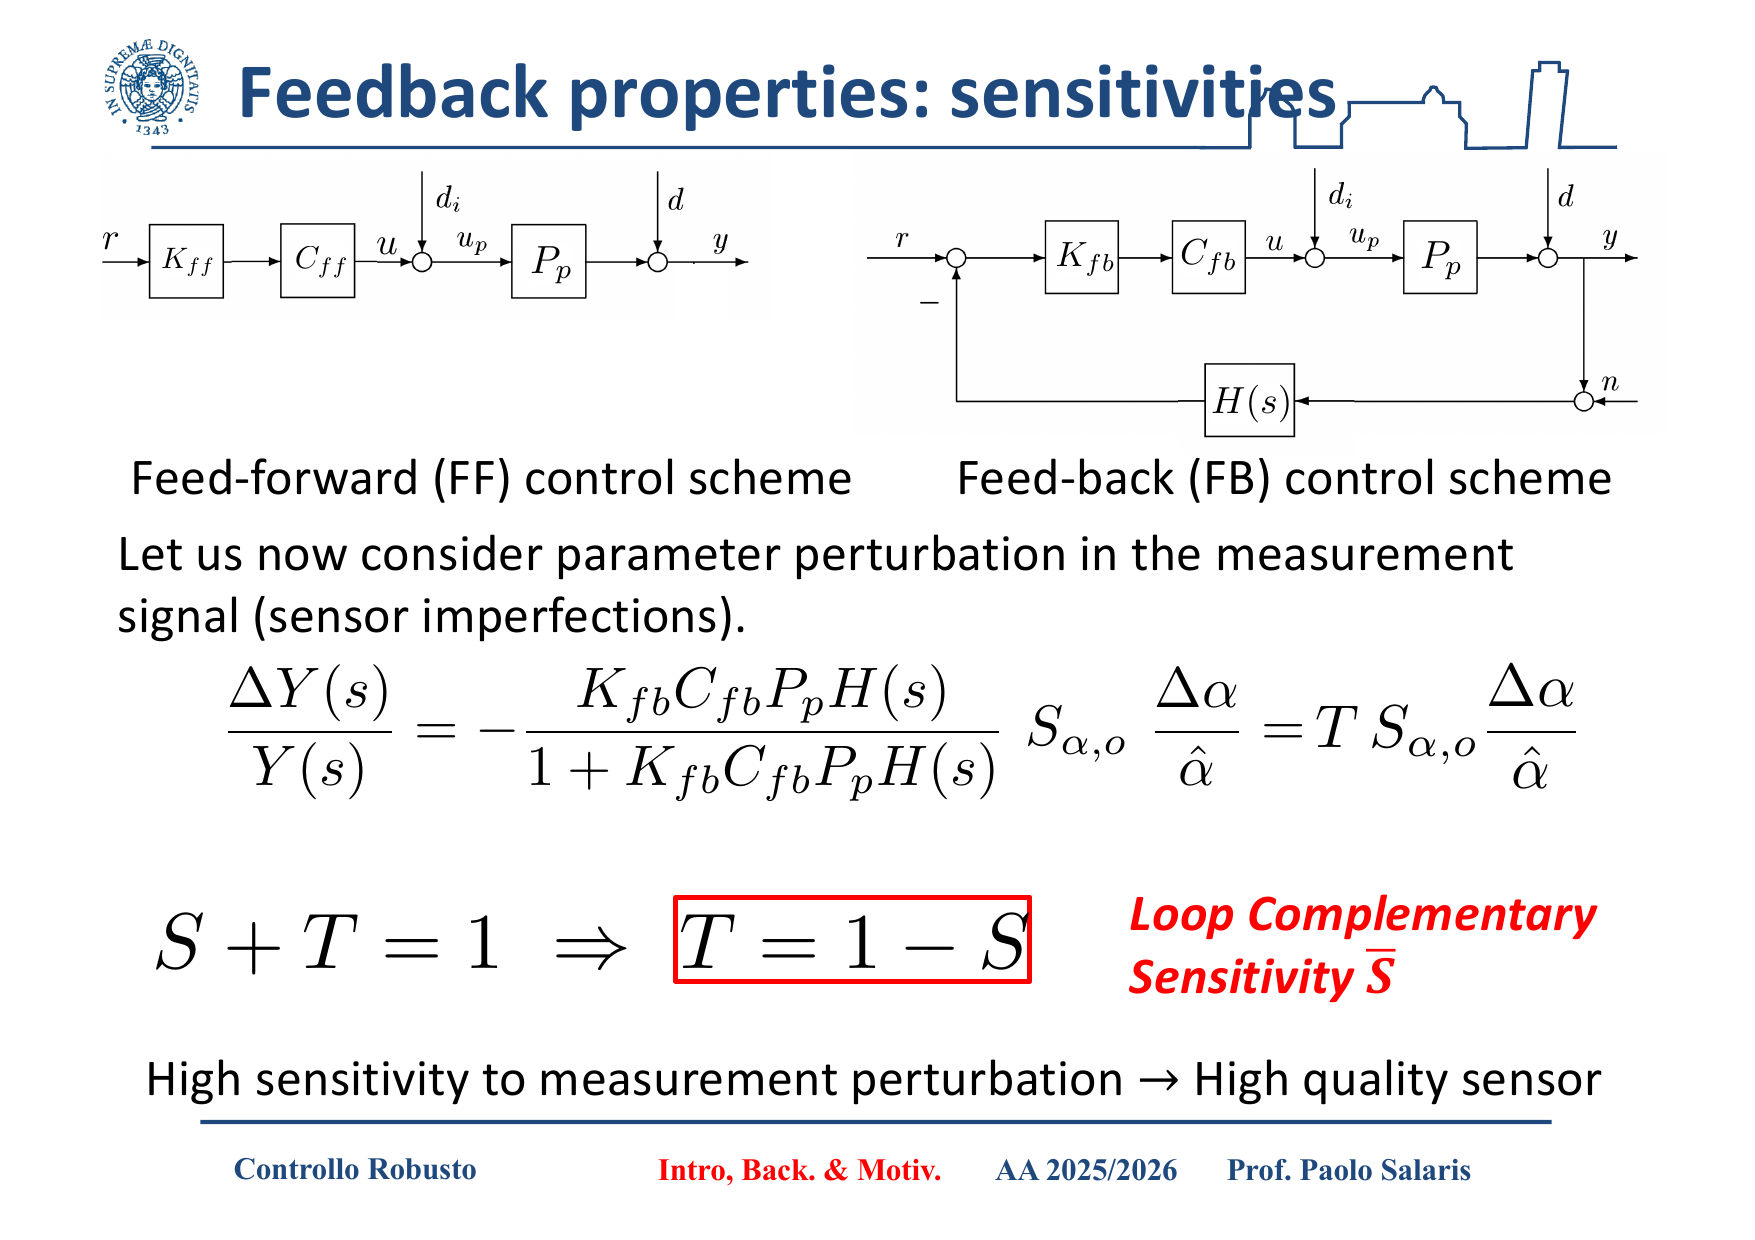
\includegraphics[width=0.8\textwidth]{images3/slide-04.png}
    \caption{Le imperfezioni del sensore mettono in evidenza il ruolo complementare di $S$ e $T$.}
\end{figure}

\begin{figure}[H]
    \centering
    \begin{subfigure}{0.48\textwidth}
        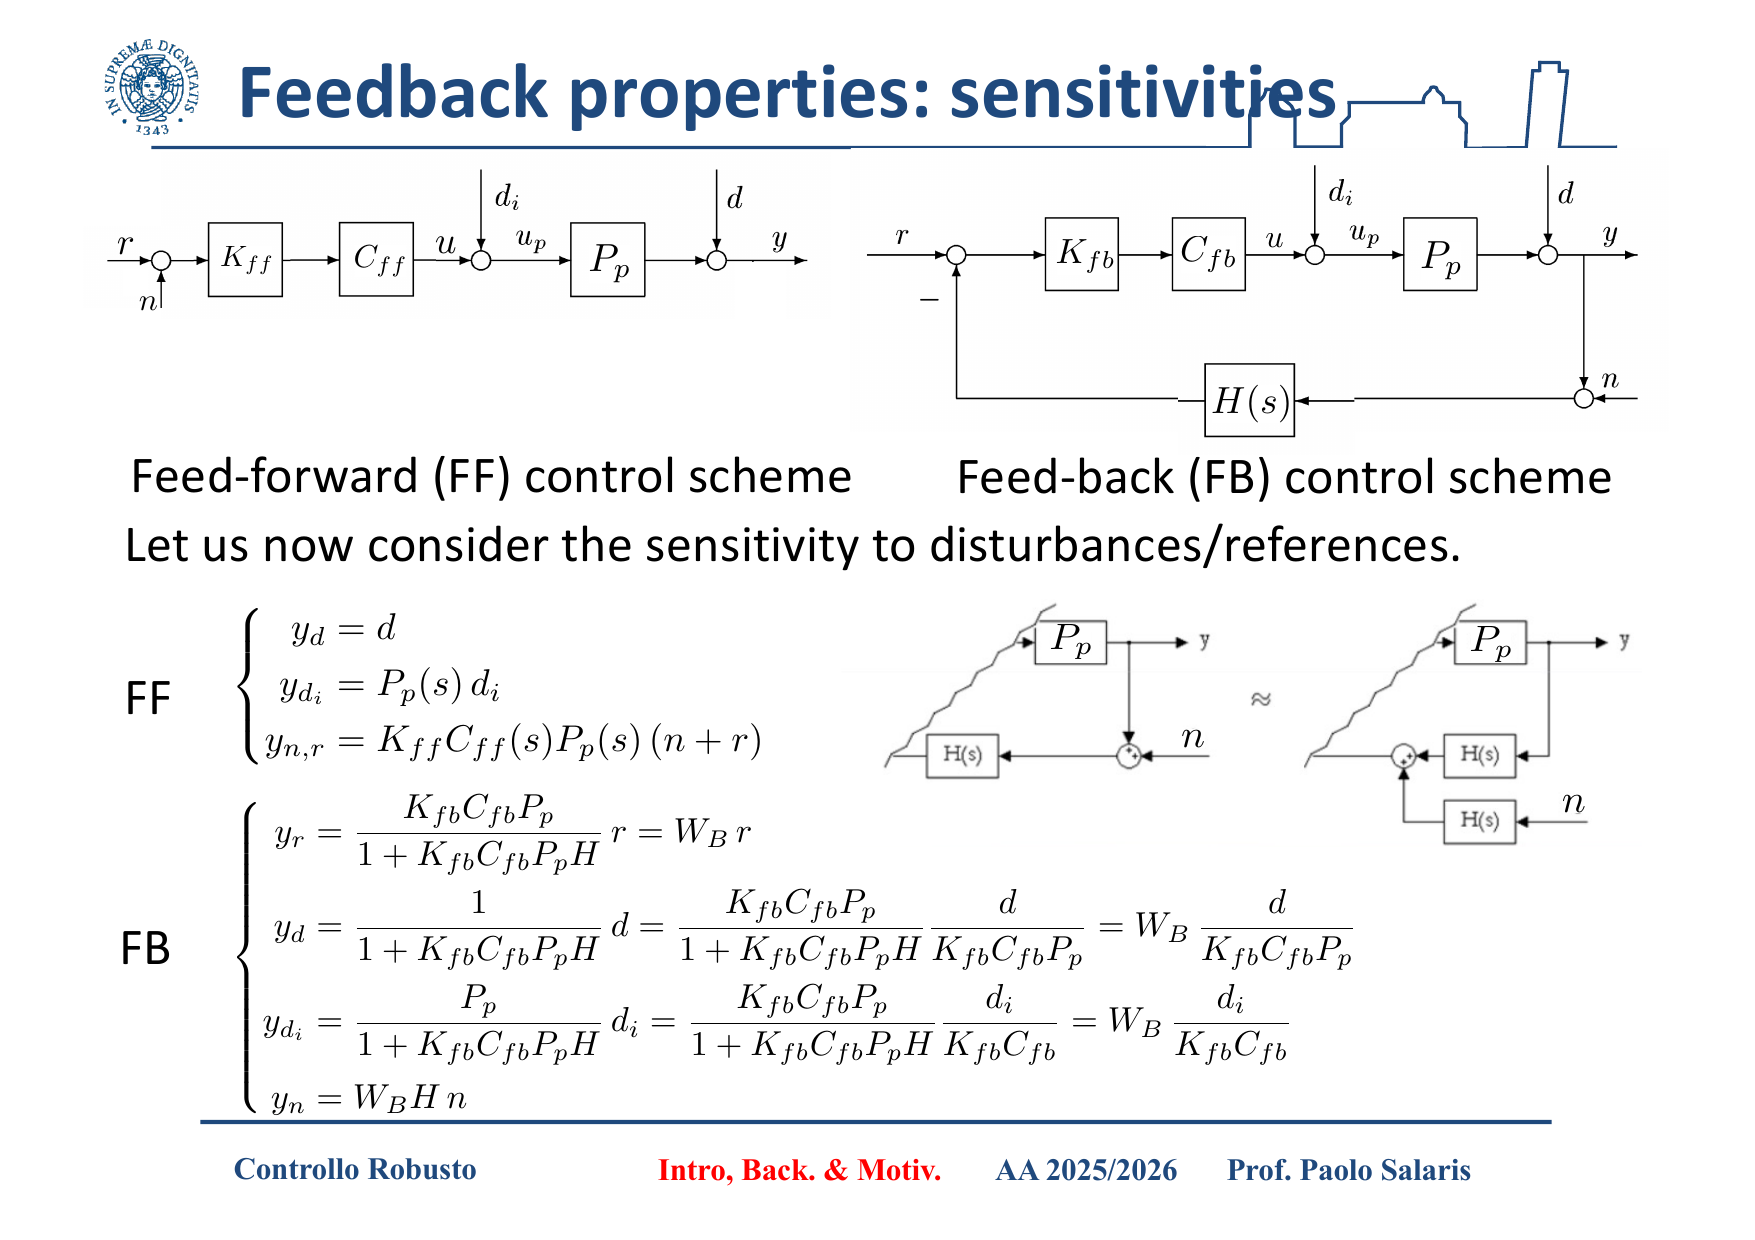
\includegraphics[width=\linewidth]{images3/slide-05.png}
        \caption{Riferimento e disturbi vengono filtrati da canali chiusi diversi.}
    \end{subfigure}
    \hfill
    \begin{subfigure}{0.48\textwidth}
        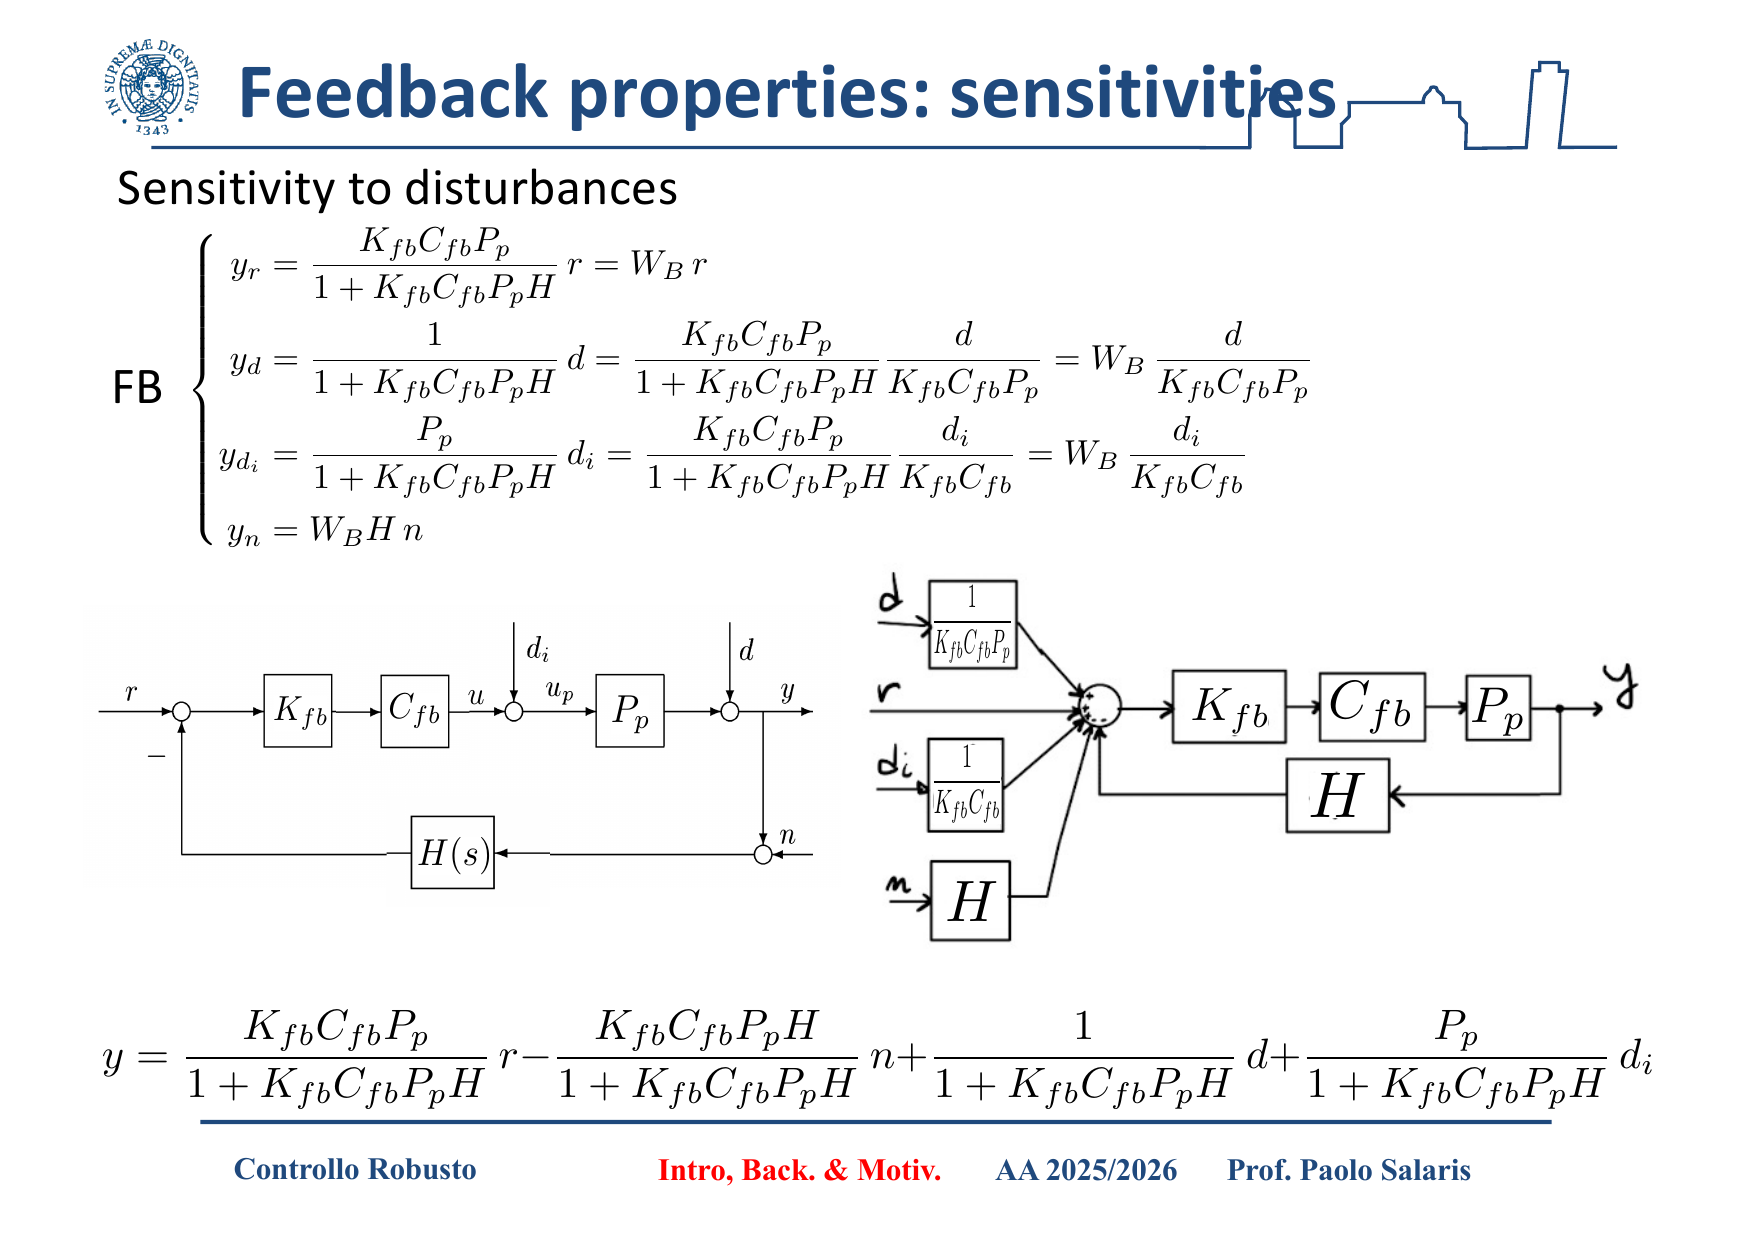
\includegraphics[width=\linewidth]{images3/slide-06.png}
        \caption{L’uscita può essere scomposta in contributi governati da $S$ e $T$.}
    \end{subfigure}
    \caption{Le mappe chiuse chiariscono subito quali quantità devono essere piccole o grandi nelle varie bande di frequenza.}
\end{figure}

\begin{figure}[H]
    \centering
    \begin{subfigure}{0.48\textwidth}
        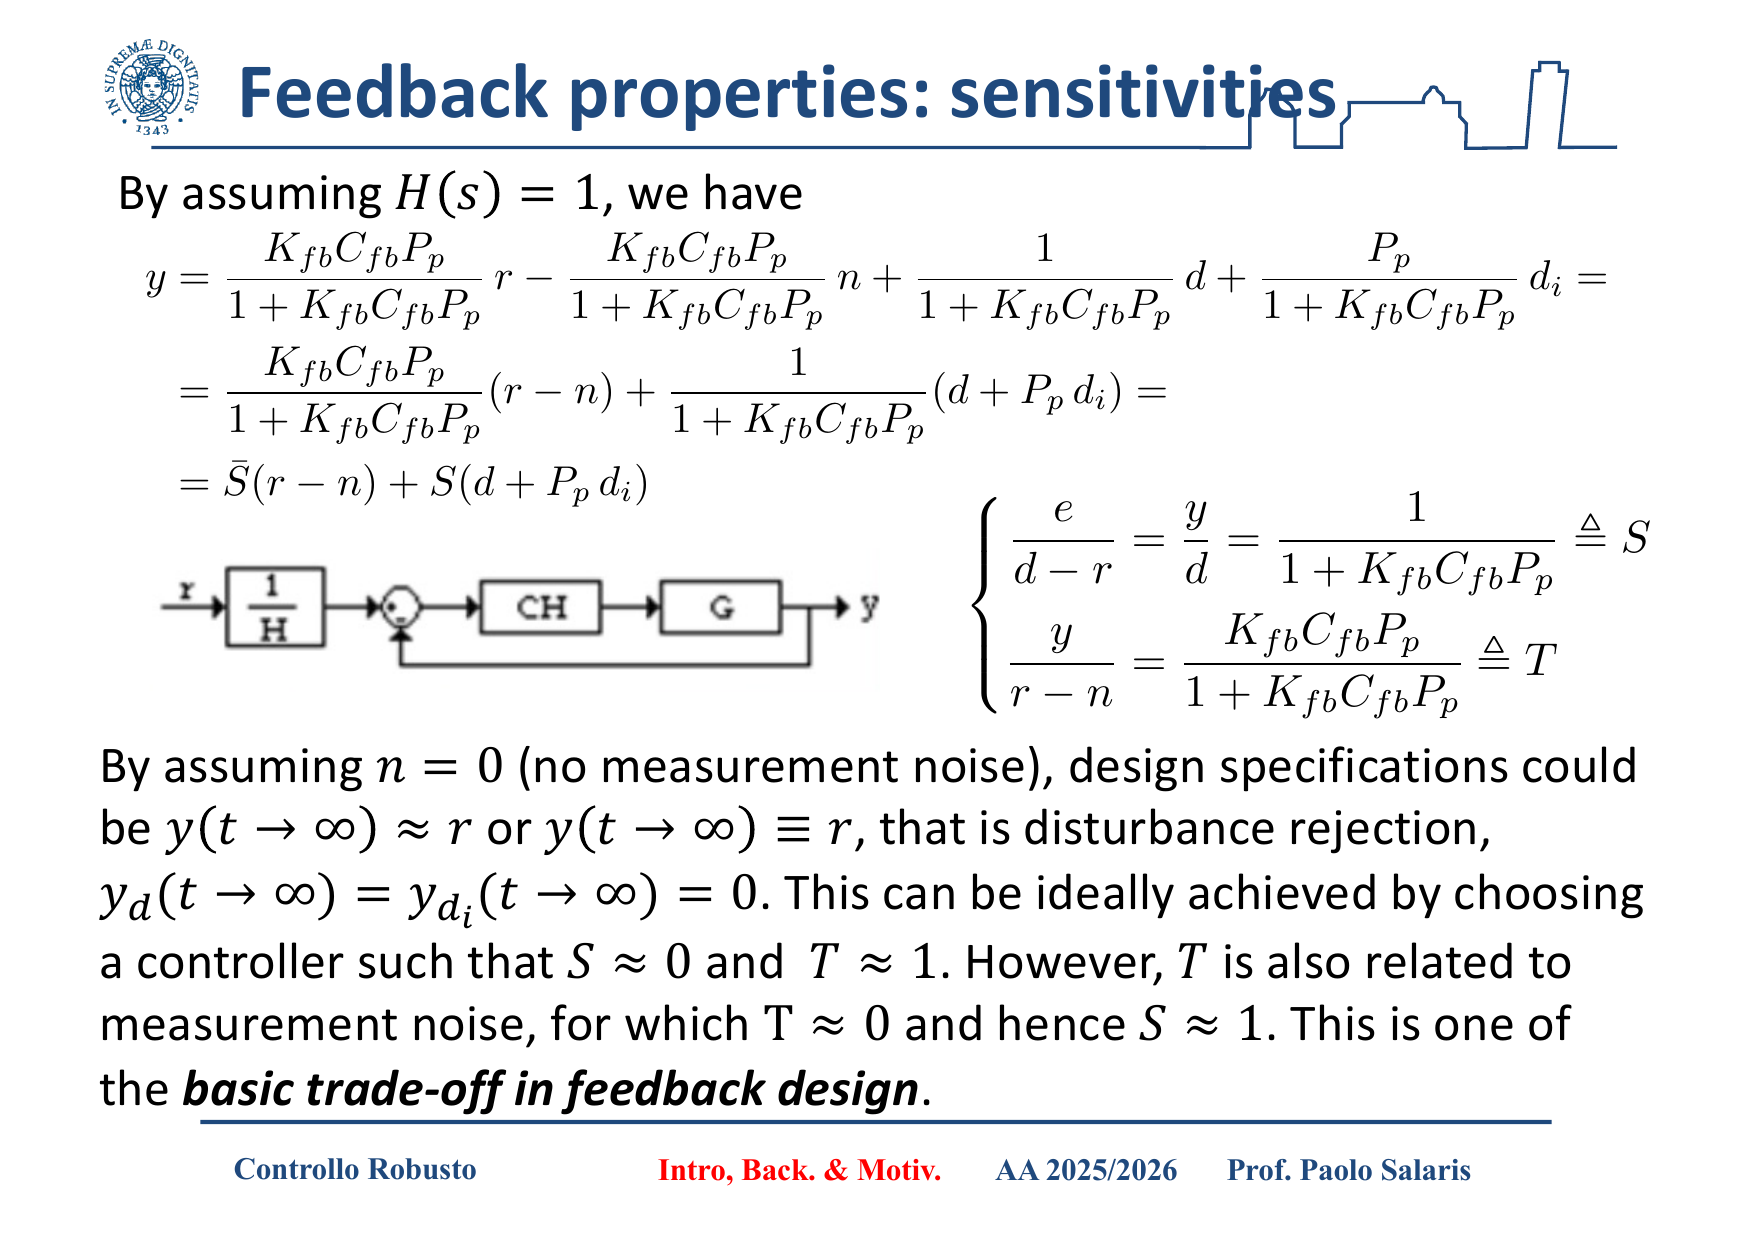
\includegraphics[width=\linewidth]{images3/slide-07.png}
        \caption{Con $H(s)=1$ le relazioni chiuse assumono una forma particolarmente trasparente.}
    \end{subfigure}
    \hfill
    \begin{subfigure}{0.48\textwidth}
        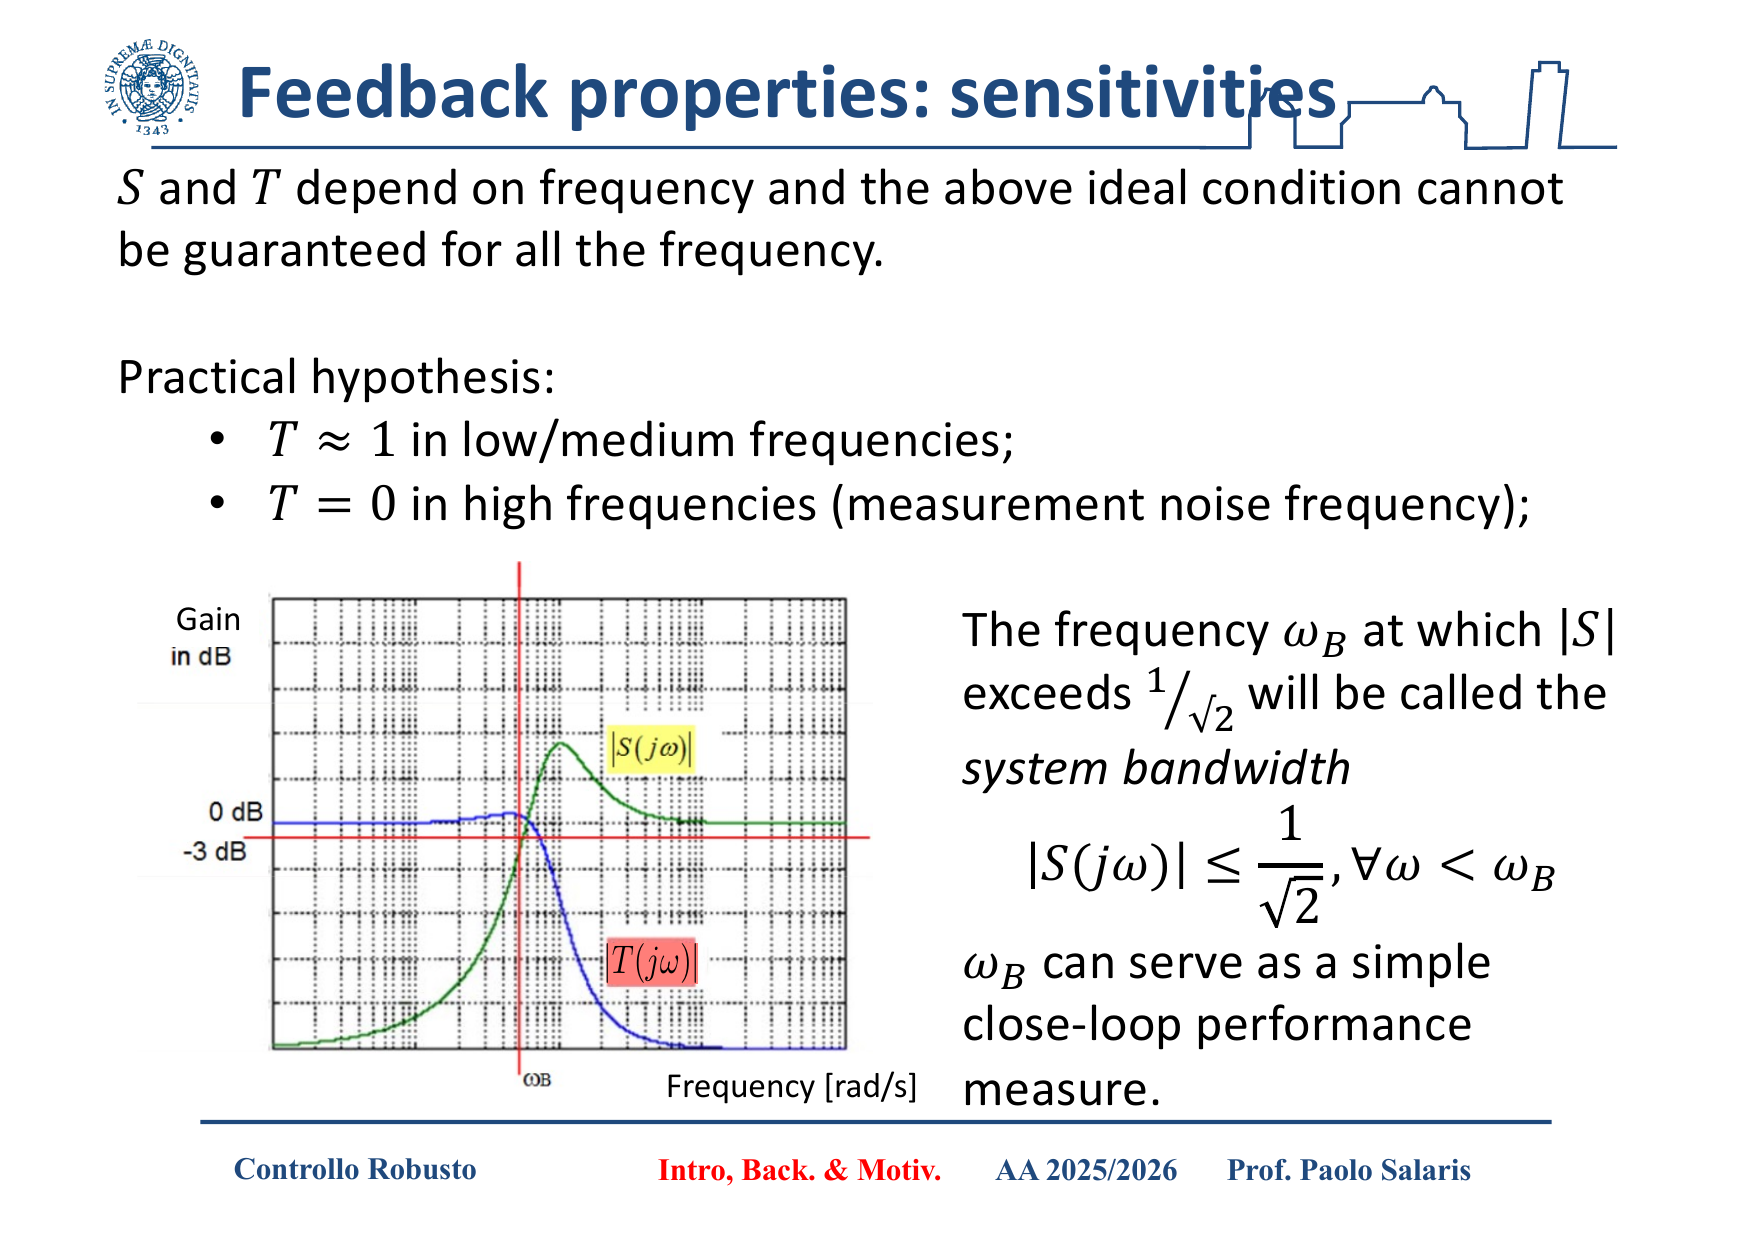
\includegraphics[width=\linewidth]{images3/slide-08.png}
        \caption{La banda passante del chiuso emerge come sintesi del compromesso fra prestazione e rumore.}
    \end{subfigure}
    \caption{Il blocco centrale della lezione traduce tracking, rigetto dei disturbi e attenuazione del rumore in specifiche di sensitività distribuite in frequenza.}
\end{figure}

\subsection{Perché un solo grado di libertà non basta}

La discussione precedente fa emergere anche un limite strutturale del controllo a un solo grado di libertà. Nella notazione delle slide, riferimento e disturbo agiscono sul medesimo errore attraverso la stessa funzione di sensitività:
$$
e = S(d-r).
$$
Al di là della convenzione di segno, il punto essenziale è che i due obiettivi restano accoppiati. Se si modifica il loop per migliorare il tracking del riferimento, si modifica automaticamente anche il modo in cui il sistema rigetta il disturbo; se si privilegia il rigetto dei disturbi, si altera inevitabilmente anche il canale del riferimento.

È qui che entra in gioco il controllo a due gradi di libertà. L’idea è separare il più possibile i ruoli: il blocco di feedback viene scelto anzitutto per garantire stabilità interna, robustezza e rigetto dei disturbi, mentre un prefiltro sul riferimento viene usato per modellare il tracking nominale. Questo non significa che i due problemi diventino completamente indipendenti, ma che si evita di far gravare sul solo loop principale sia l’intero problema della robustezza sia l’intero problema della forma della risposta al set-point.

Il vantaggio concettuale è importante anche in vista della Lezione 5. Quando più avanti si parlerà di loop shaping, il loop principale verrà progettato soprattutto in funzione di $S$ e $T$, cioè della robustezza e della distribuzione delle prestazioni in frequenza. Il canale del riferimento potrà invece essere sagomato separatamente, senza costringere il feedback a un compromesso inutilmente penalizzante.

\begin{figure}[H]
    \centering
    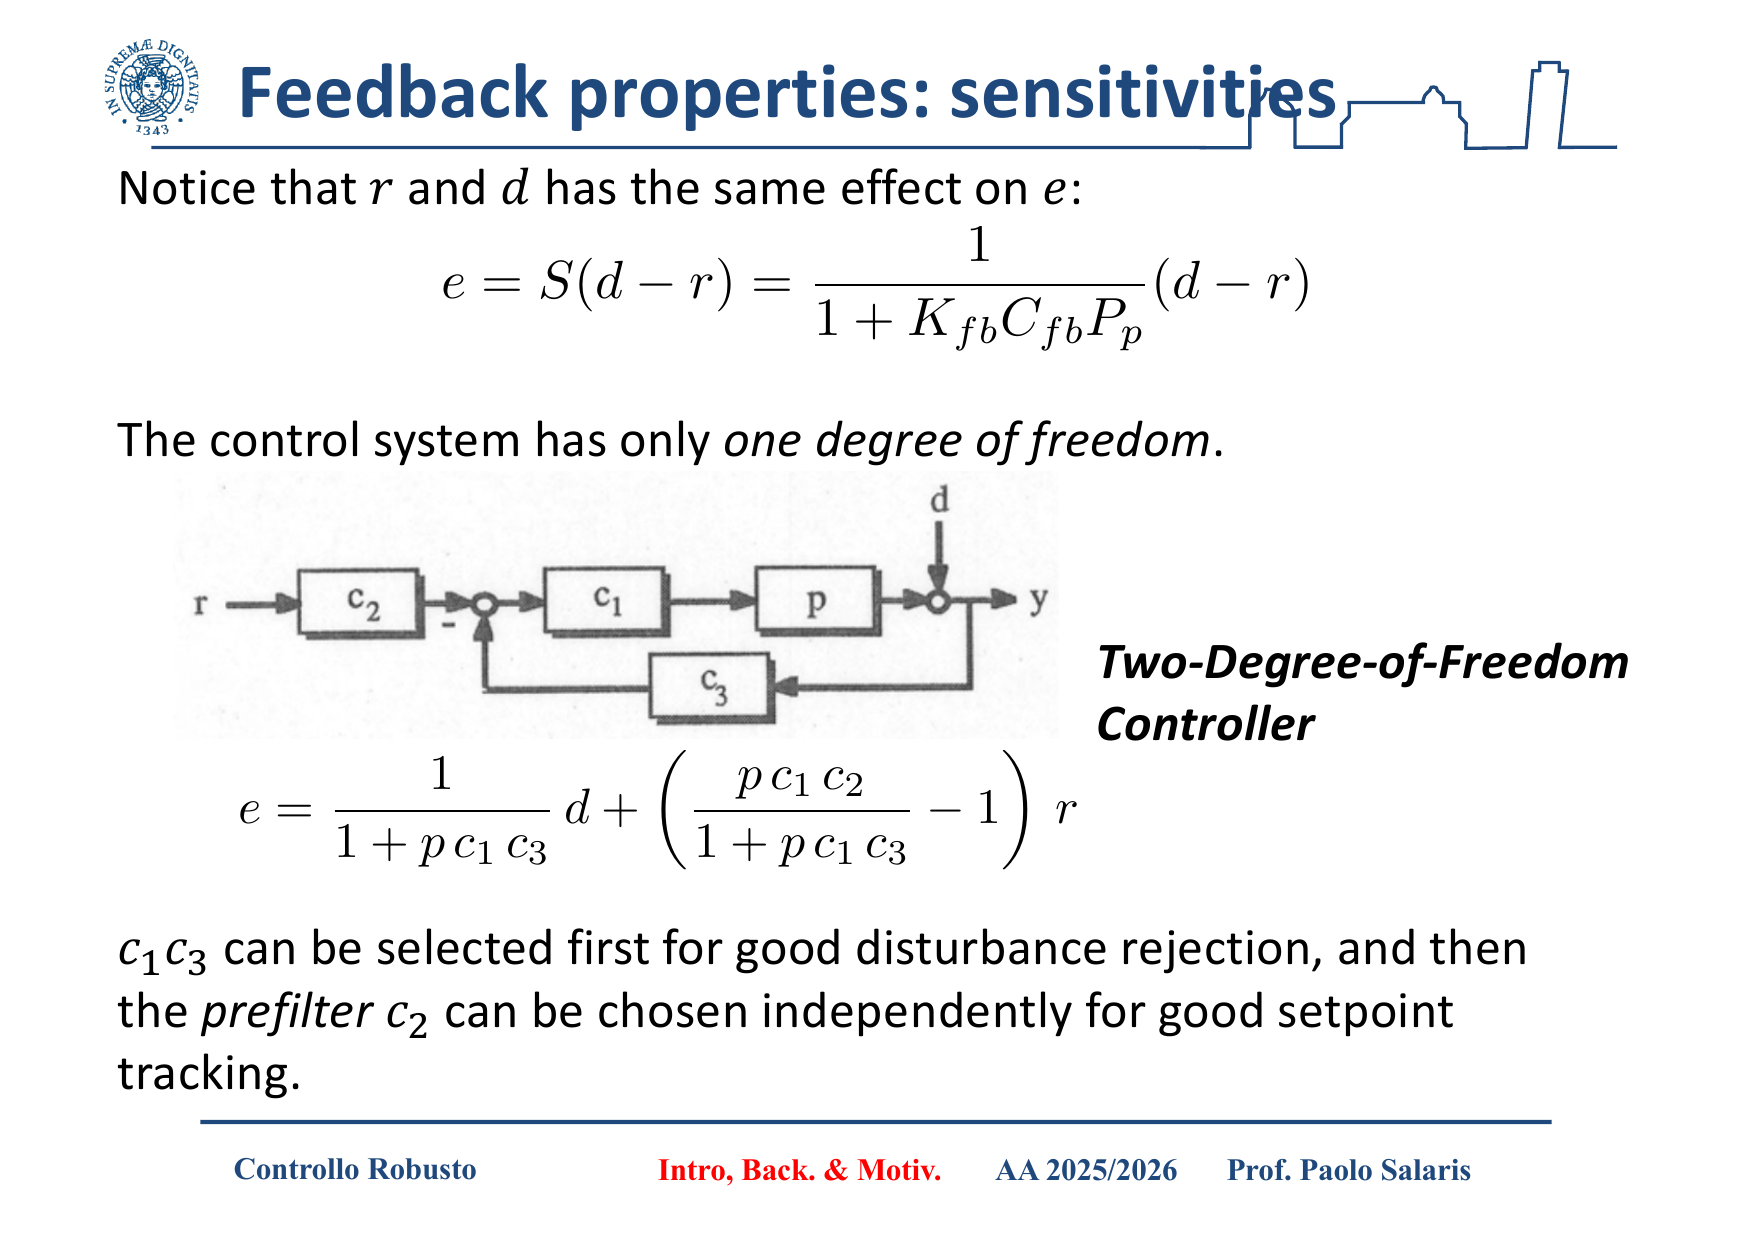
\includegraphics[width=0.78\textwidth]{images3/slide-09.png}
    \caption{La struttura a due gradi di libertà consente di trattare più separatamente rigetto dei disturbi e tracking del riferimento.}
\end{figure}

\subsection{Le matrici di sensitività nel caso MIMO}

Passando al caso multivariabile, le idee non cambiano ma il linguaggio sì. Nel caso SISO le quantità di interesse sono numeri complessi e il prodotto d’anello è univoco; nel caso MIMO, invece, ingresso e uscita sono vettori e l’ordine dei prodotti conta. Per questo la lezione introduce due matrici di loop transfer:
$$
L_i = KP,
\qquad
L_o = PK,
$$
chiamate rispettivamente \emph{input loop transfer matrix} e \emph{output loop transfer matrix}. A esse corrispondono due coppie di matrici di sensitività:
$$
S_i=(I+L_i)^{-1},
\qquad
T_i=I-S_i=L_i(I+L_i)^{-1},
$$
$$
S_o=(I+L_o)^{-1},
\qquad
T_o=I-S_o=L_o(I+L_o)^{-1}.
$$

Nel caso SISO input e output loop coincidono; nel MIMO no, ma descrivono lo stesso ciclo chiuso da due punti di vista complementari. Questo si vede anche da identità molto utili:
$$
S_oP = PS_i,
\qquad
KS_o = S_iK,
$$
che mostrano come le mappe viste dal lato dell’uscita e quelle viste dal lato dell’ingresso restino coerenti fra loro.

Se il sistema è internamente stabile, le slide raccolgono i segnali chiusi nelle relazioni
\begin{align*}
y &= T_o(r-n)+S_oPd_i+S_od, \\
r-y &= S_o(r-d)+T_on-S_oPd_i, \\
u &= KS_i(r-n)-KS_od-T_id_i, \\
u_p &= KS_i(r-n)-KS_od+S_id_i.
\end{align*}
Queste formule meritano di essere lette con attenzione, perché anticipano già il contenuto della Lezione 5. Il disturbo in uscita viene filtrato da $S_o$; il disturbo in ingresso al processo coinvolge $S_i$ e $S_oP$; il rumore di misura passa attraverso $T_o$; il segnale di controllo dipende dal modo in cui il feedback trasforma riferimento, disturbi e rumore prima ancora che essi raggiungano il processo.

La differenza rispetto al caso SISO è che ora dire ``rendere piccolo un canale'' non basta più. Una matrice può essere piccola in alcune direzioni e grande in altre. Proprio per questo, subito dopo aver introdotto $S_i$, $S_o$, $T_i$ e $T_o$, la lezione deve chiarire \emph{come} si misura il guadagno di una matrice di trasferimento. È questa la porta d’ingresso al tema dei valori singolari.

\begin{figure}[H]
    \centering
    \begin{subfigure}{0.48\textwidth}
        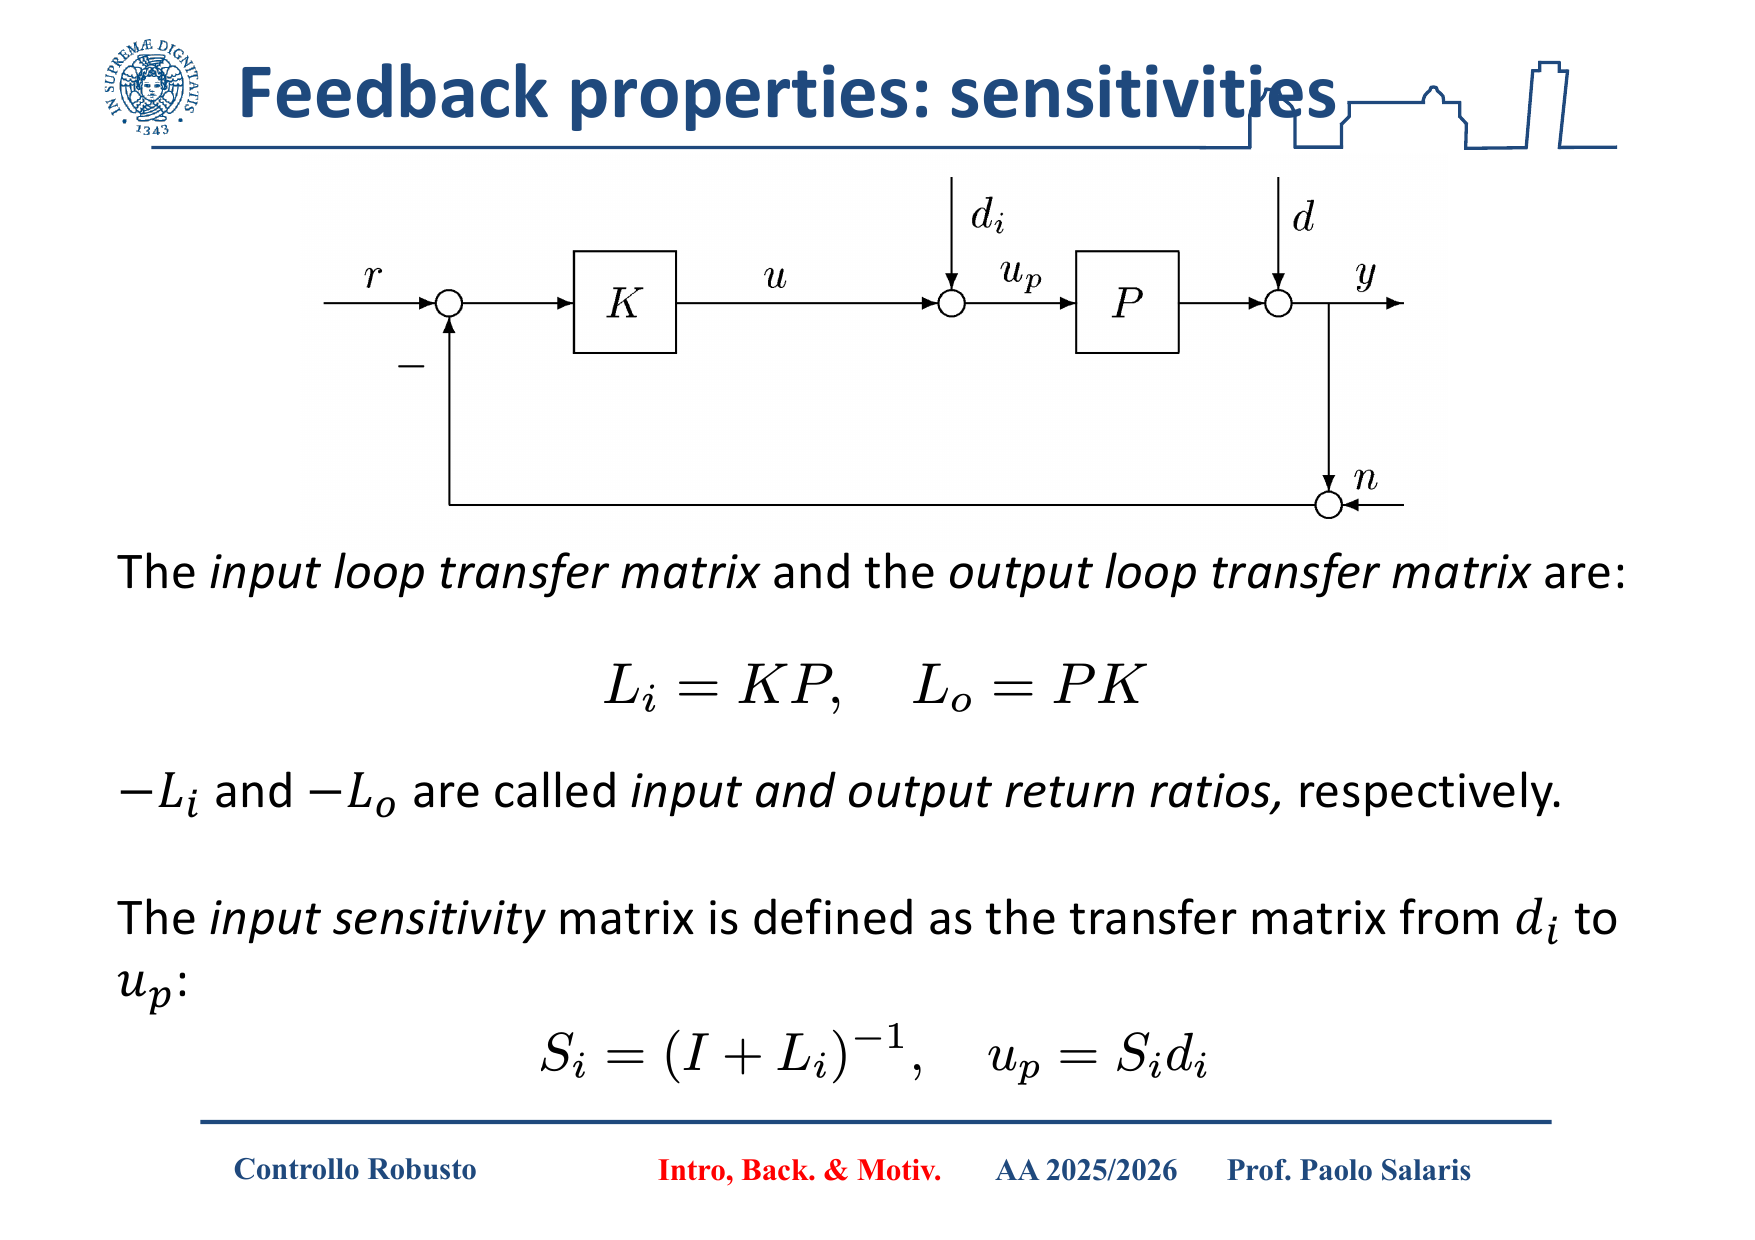
\includegraphics[width=\linewidth]{images3/slide-10.png}
        \caption{Le matrici di anello dal lato dell’ingresso e dal lato dell’uscita non coincidono più.}
    \end{subfigure}
    \hfill
    \begin{subfigure}{0.48\textwidth}
        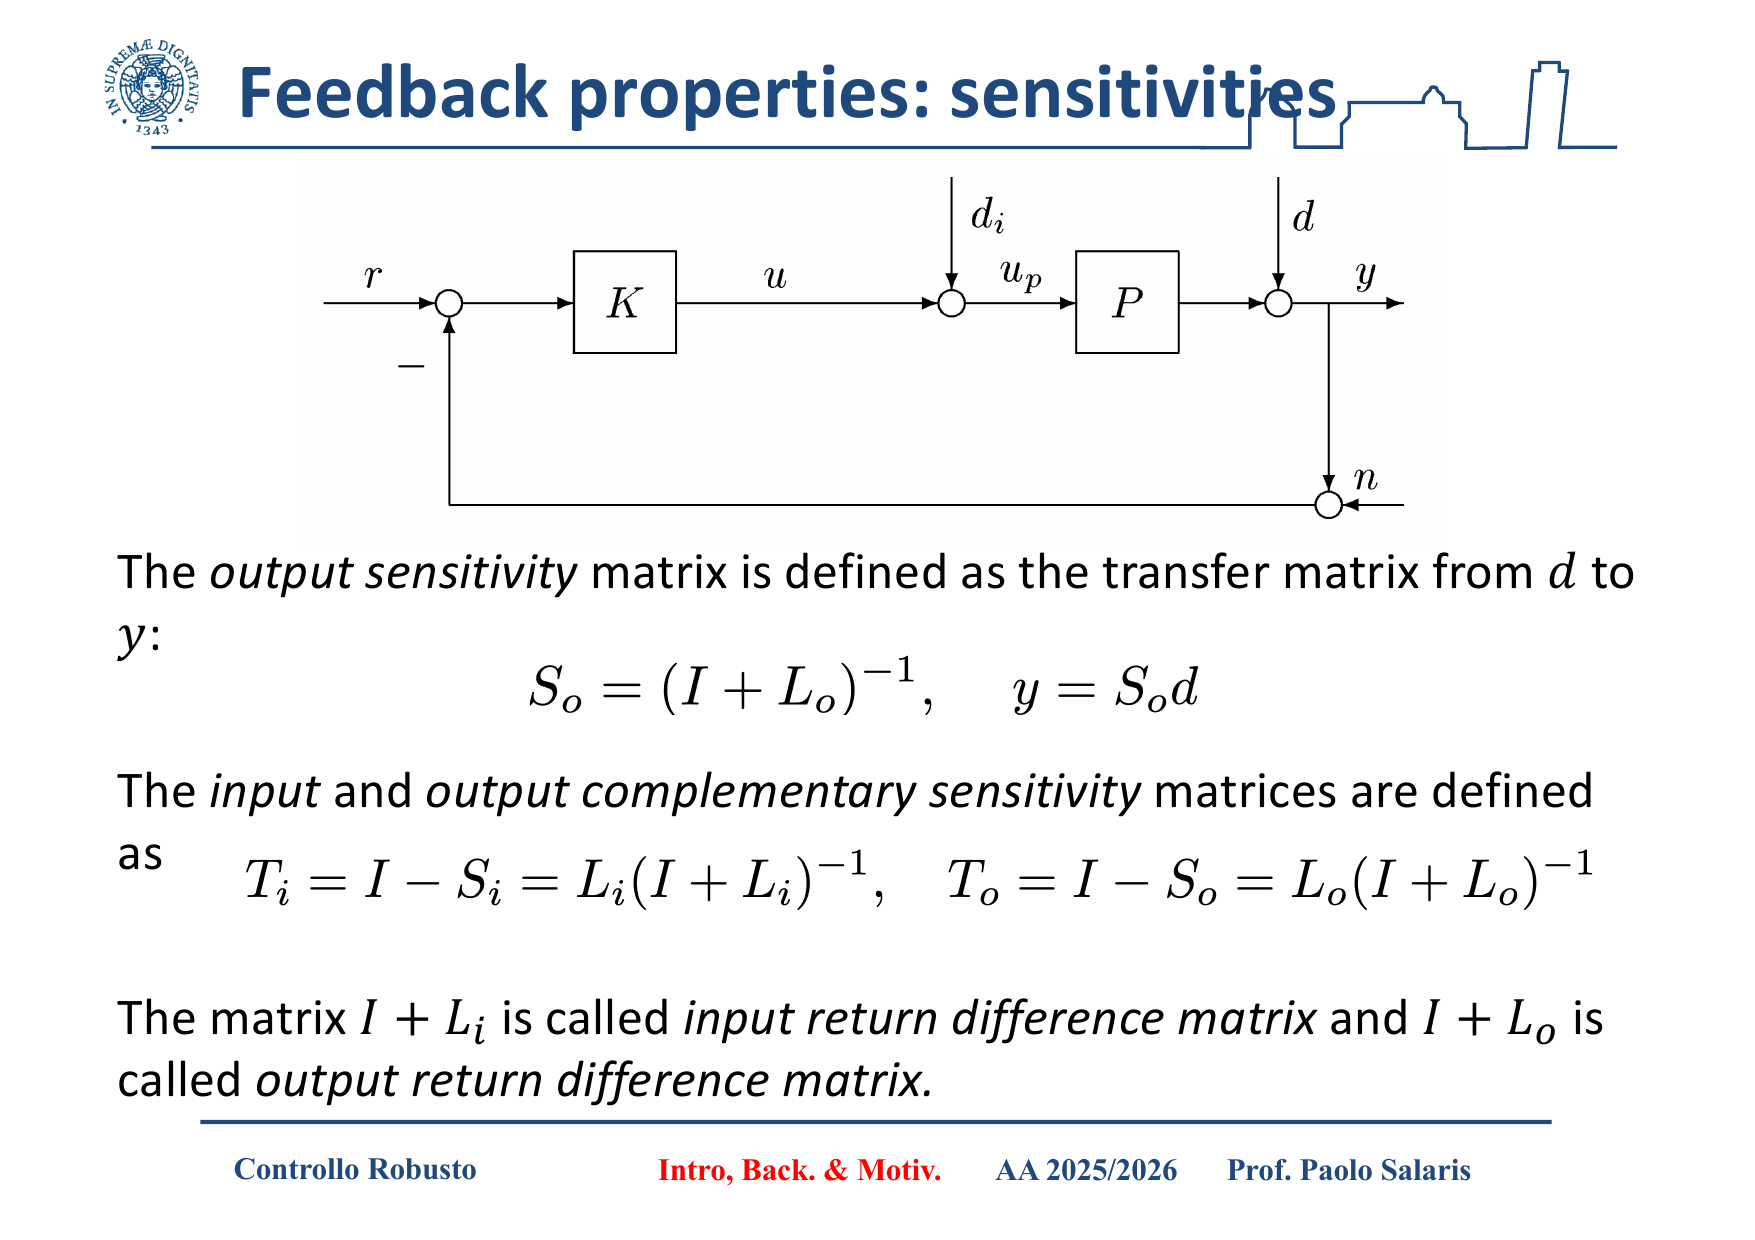
\includegraphics[width=\linewidth]{images3/slide-11.png}
        \caption{Le matrici di sensitività e sensitività complementare generalizzano esattamente il caso SISO.}
    \end{subfigure}
    \caption{Nel MIMO il linguaggio di $S$ e $T$ sopravvive, ma si arricchisce di struttura matriciale.}
\end{figure}

\begin{figure}[H]
    \centering
    \begin{subfigure}{0.48\textwidth}
        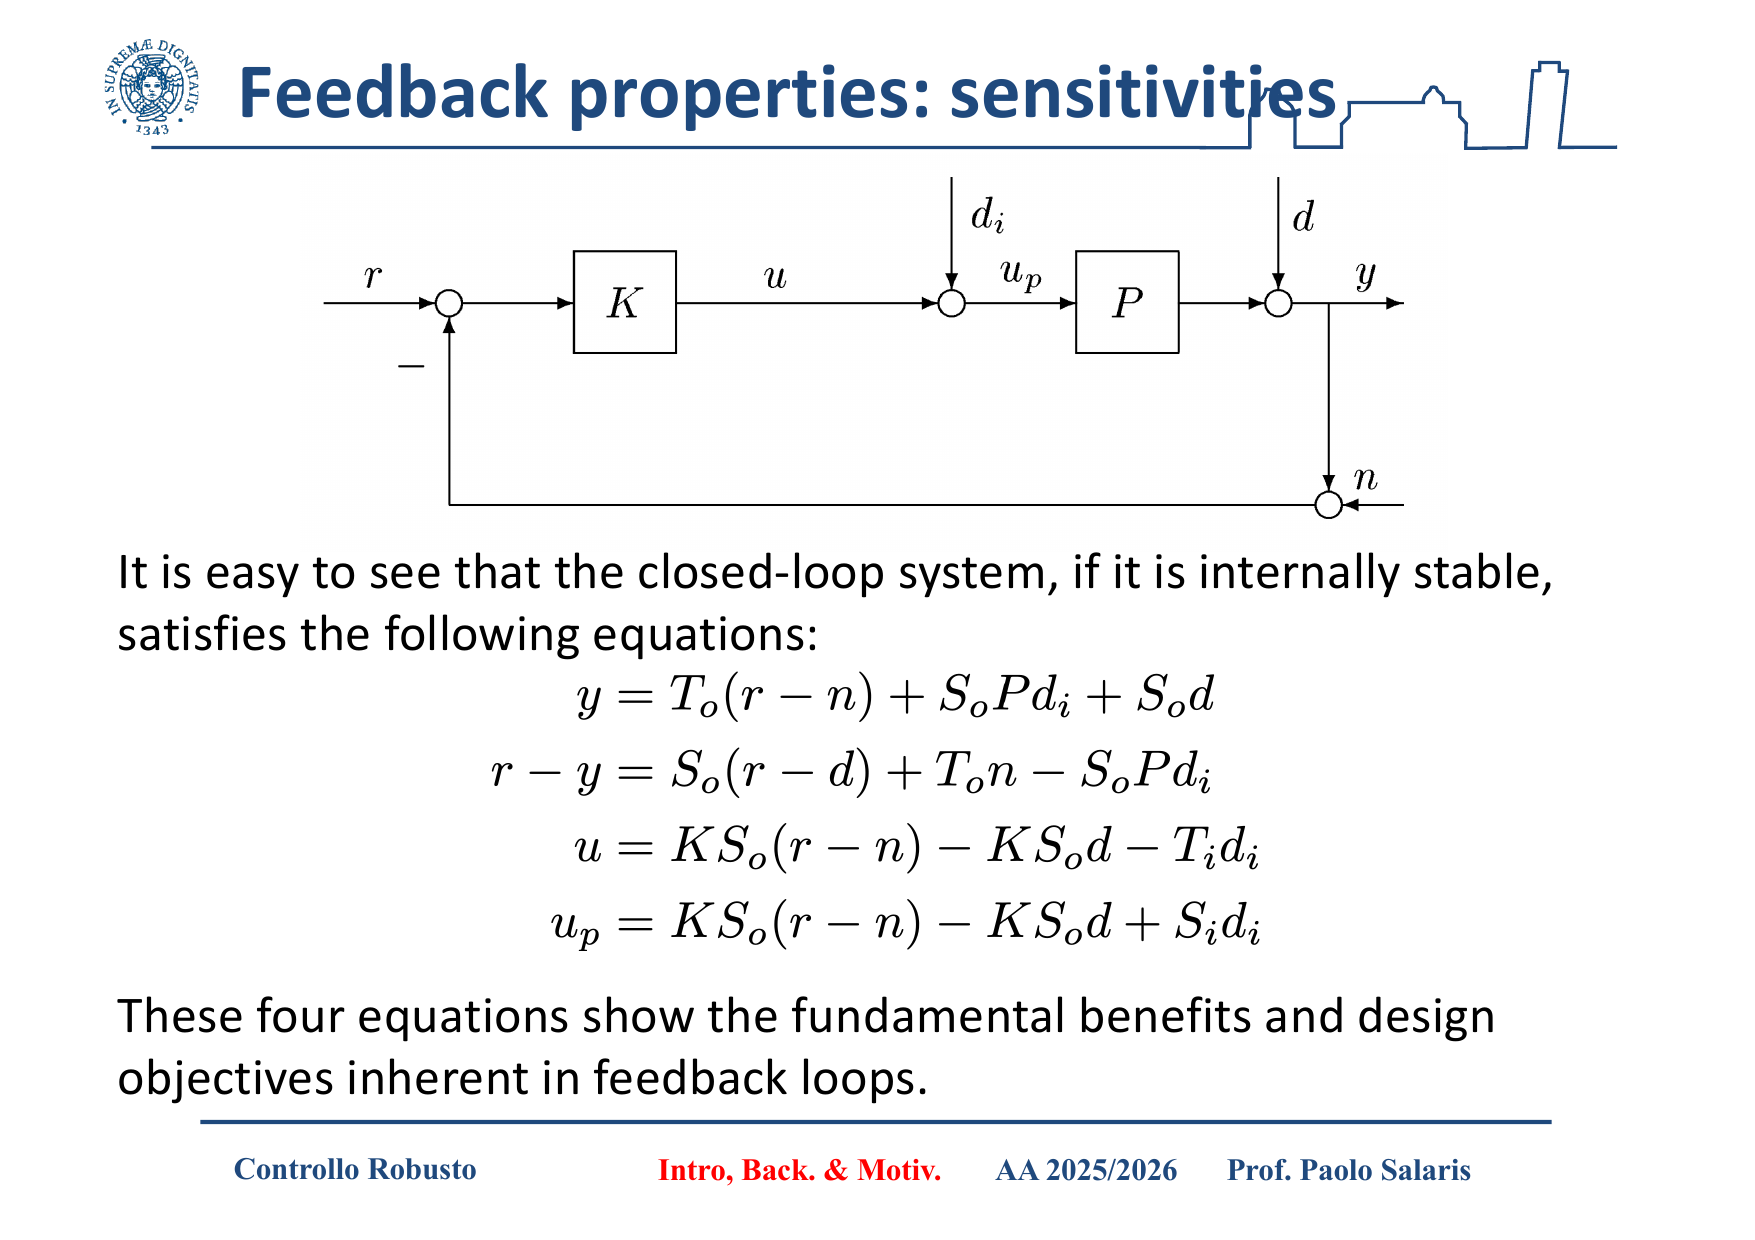
\includegraphics[width=\linewidth]{images3/slide-12.png}
        \caption{Le mappe chiuse mostrano attraverso quali matrici passano riferimento, disturbi e rumore.}
    \end{subfigure}
    \hfill
    \begin{subfigure}{0.48\textwidth}
        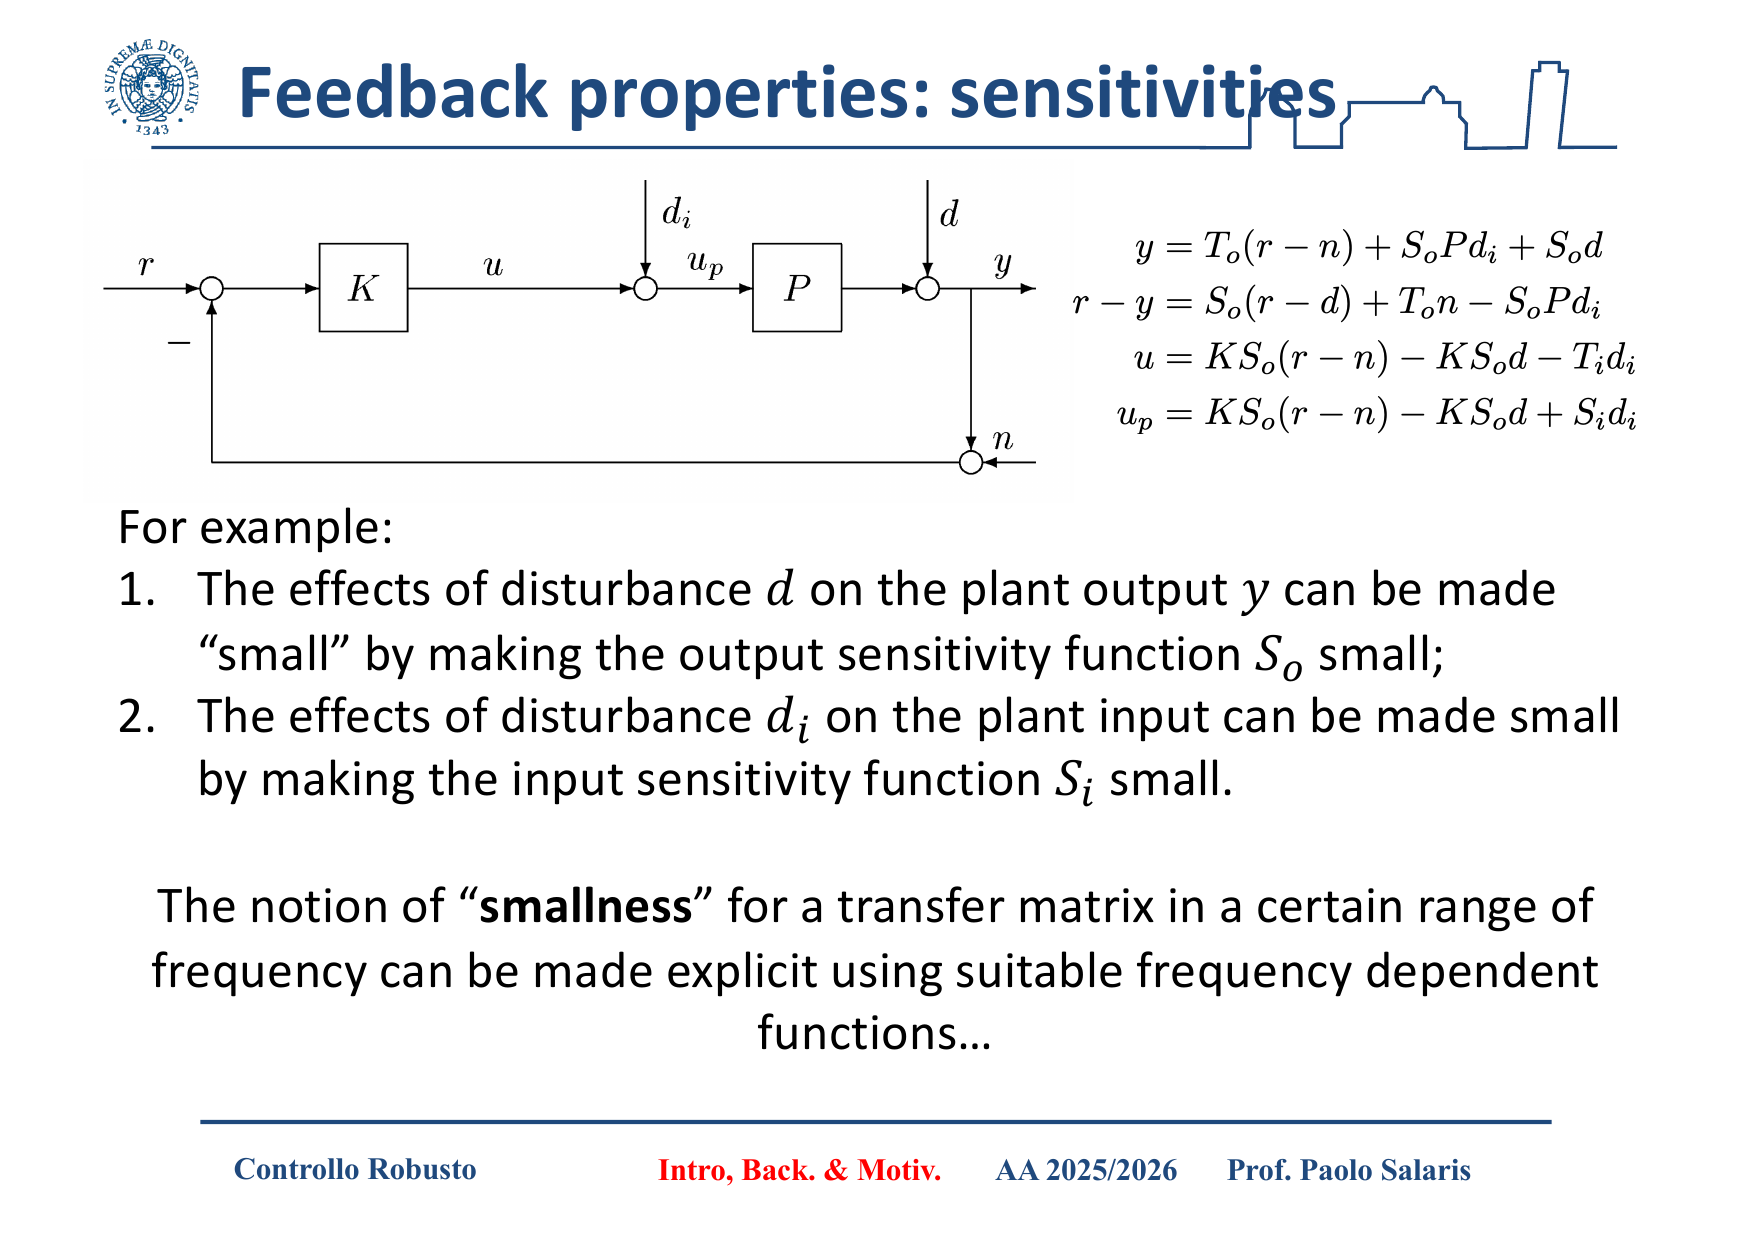
\includegraphics[width=\linewidth]{images3/slide-13.png}
        \caption{Le quattro relazioni chiuse si traducono immediatamente in obiettivi di progetto.}
    \end{subfigure}
    \caption{La generalizzazione MIMO di $S$ e $T$ prepara direttamente il terreno alla lettura per guadagni principali della Lezione 5.}
\end{figure}

\subsection{Risposta in frequenza multivariabile e guadagno direzionale}

La parte successiva della lezione spiega perché, nei sistemi multivariabili, la tradizionale lettura ``canale per canale'' non sia più sufficiente. Per un ingresso sinusoidale vettoriale a frequenza fissata $\omega$, la risposta si scrive
$$
y(j\omega)=G(j\omega)d(j\omega).
$$
Ogni elemento $g_{ij}(j\omega)$ continua a descrivere come l’ingresso $j$ influenzi l’uscita $i$, ma questa descrizione parziale non dice ancora quali combinazioni simultanee di ingressi producano l’effetto più grande o più piccolo sul vettore di uscita.

È qui che appare la nozione corretta di guadagno MIMO. Se si usa la norma euclidea per misurare ampiezza di ingressi e uscite, il guadagno a frequenza fissata non è più il semplice modulo di una funzione scalare, ma il rapporto
$$
\frac{\|G(j\omega)d\|_2}{\|d\|_2}.
$$
A differenza del caso SISO, tale quantità dipende non solo dalla frequenza ma anche dalla direzione del vettore $d$. Due ingressi con la stessa norma possono infatti produrre uscite di norma molto diversa se sono orientati in direzioni differenti nello spazio degli ingressi.

Questa osservazione è il vero cuore della risposta in frequenza MIMO. La matrice dinamica non si limita a amplificare o ritardare i segnali: \emph{ruota} le direzioni di ingresso e le deforma in modo diverso a seconda della direzione considerata. Geometricamente, la sfera unitaria degli ingressi viene trasformata in un’ellisse o, in dimensione maggiore, in un ellissoide nello spazio delle uscite. Gli assi di questo ellissoide sono precisamente le direzioni in cui il sistema è più forte o più debole.

Per misurare tali direzioni si introducono massimo e minimo valore singolare:
$$
\bar{\sigma}(G)=\max_{\|d\|_2=1}\|Gd\|_2,
\qquad
\underline{\sigma}(G)=\min_{\|d\|_2=1}\|Gd\|_2.
$$
Il primo rappresenta il massimo guadagno ottenibile scegliendo la direzione peggiore dell’ingresso; il secondo rappresenta la direzione meno amplificata. Per ogni vettore vale dunque
$$
\underline{\sigma}(G)\le \frac{\|Gd\|_2}{\|d\|_2}\le \bar{\sigma}(G).
$$
Questa è la generalizzazione corretta del modulo nel caso multivariabile.

L’esempio numerico delle slide è illuminante proprio perché mostra quanto la dipendenza dalla direzione possa essere forte: cinque ingressi tutti di norma unitaria producono uscite con guadagni molto diversi. Di conseguenza, guardare solo i moduli dei singoli elementi di matrice può essere fuorviante: ciò che conta davvero è il comportamento della matrice come operatore complessivo.

In questo contesto diventa anche chiaro perché gli autovalori siano una misura povera del guadagno. Essi descrivono bene il comportamento solo nelle direzioni degli autovettori e richiedono, per di più, una matrice quadrata. I valori singolari, invece, forniscono sempre il massimo e il minimo guadagno in norma 2, hanno una chiara interpretazione energetica e si applicano anche a impianti non quadrati. Per l’analisi delle prestazioni e della robustezza, sono quindi l’oggetto naturale.

\begin{figure}[H]
    \centering
    \begin{subfigure}{0.48\textwidth}
        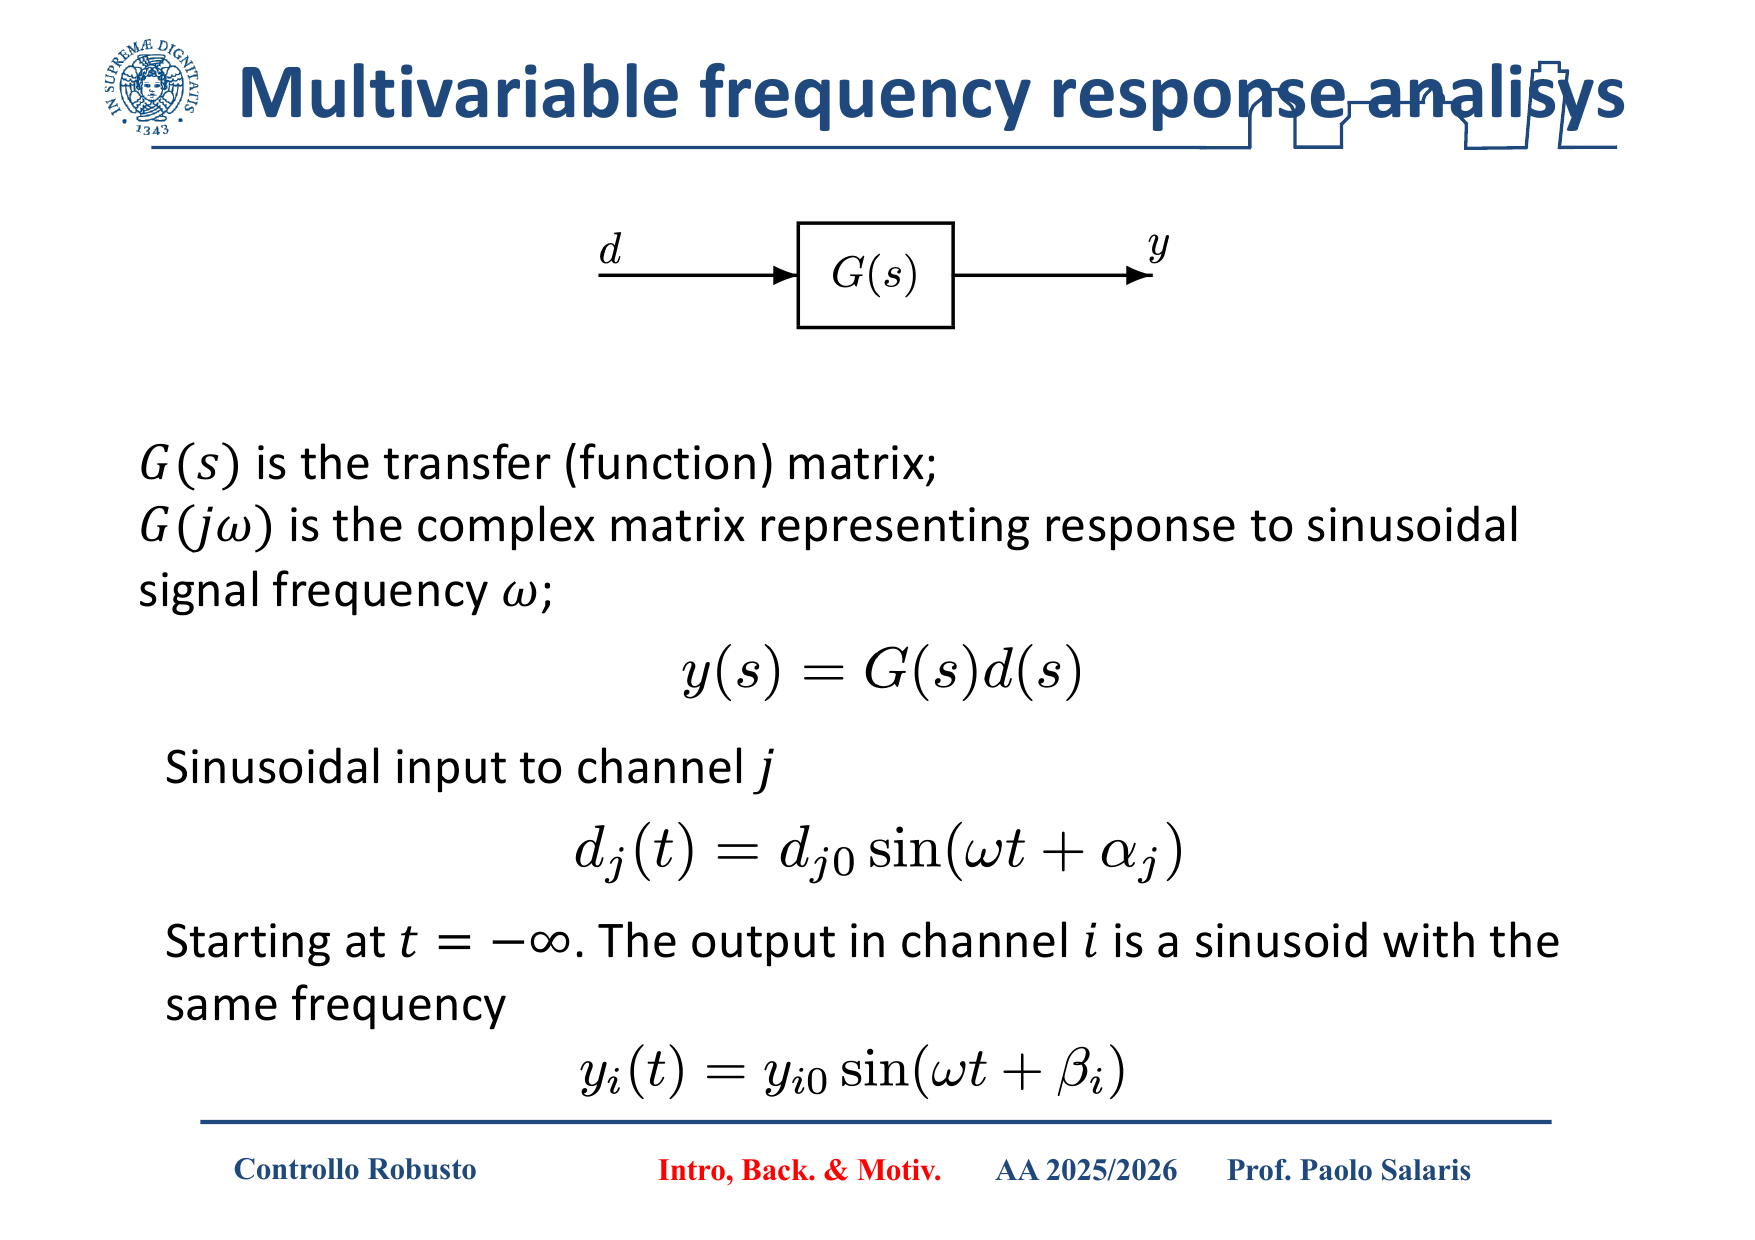
\includegraphics[width=\linewidth]{images3/slide-14.png}
        \caption{La risposta sinusoidale può essere descritta canale per canale, ma questa lettura resta parziale.}
    \end{subfigure}
    \hfill
    \begin{subfigure}{0.48\textwidth}
        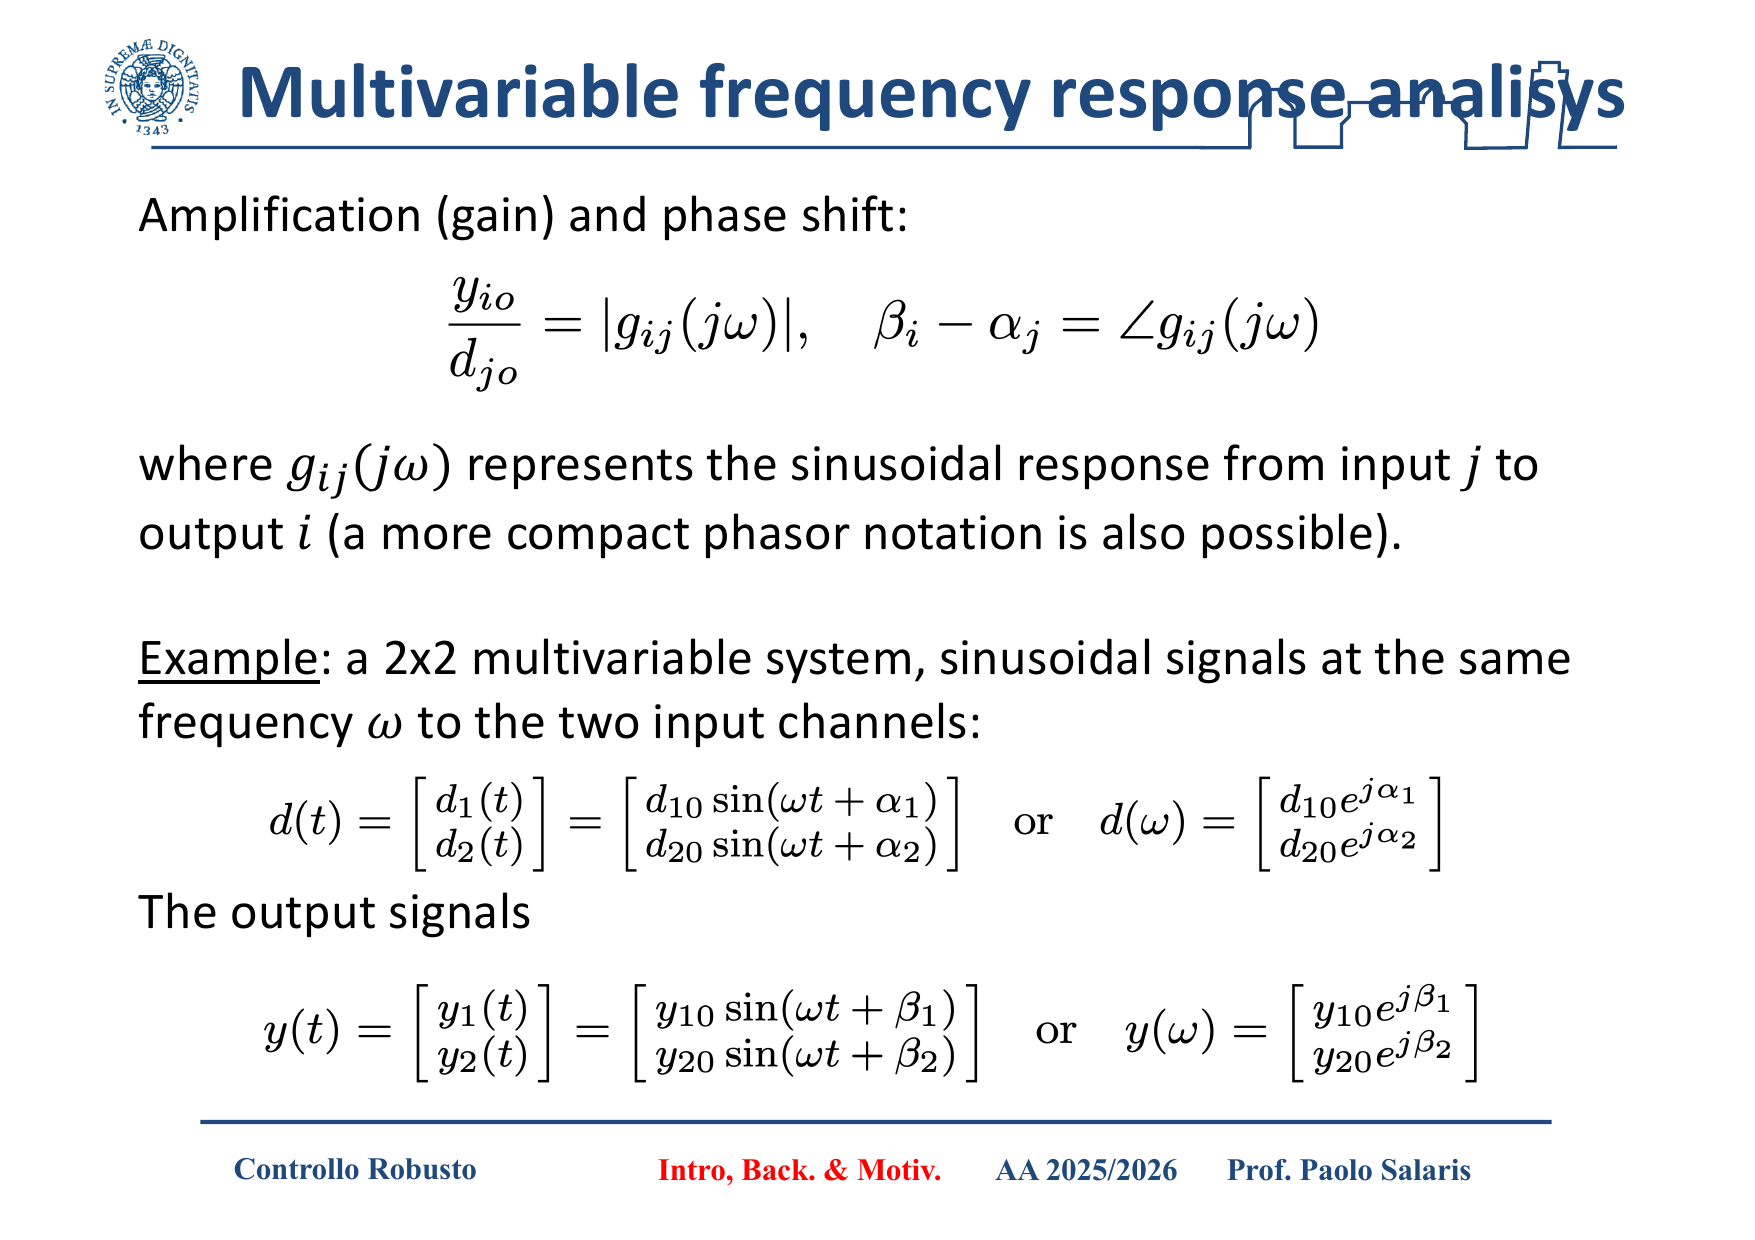
\includegraphics[width=\linewidth]{images3/slide-15.png}
        \caption{Ampiezza e fase dei singoli elementi di matrice non esauriscono il comportamento complessivo del sistema.}
    \end{subfigure}
    \caption{Le prime slide sulla risposta in frequenza MIMO mostrano i limiti di una lettura puramente elemento per elemento.}
\end{figure}

\begin{figure}[H]
    \centering
    \begin{subfigure}{0.48\textwidth}
        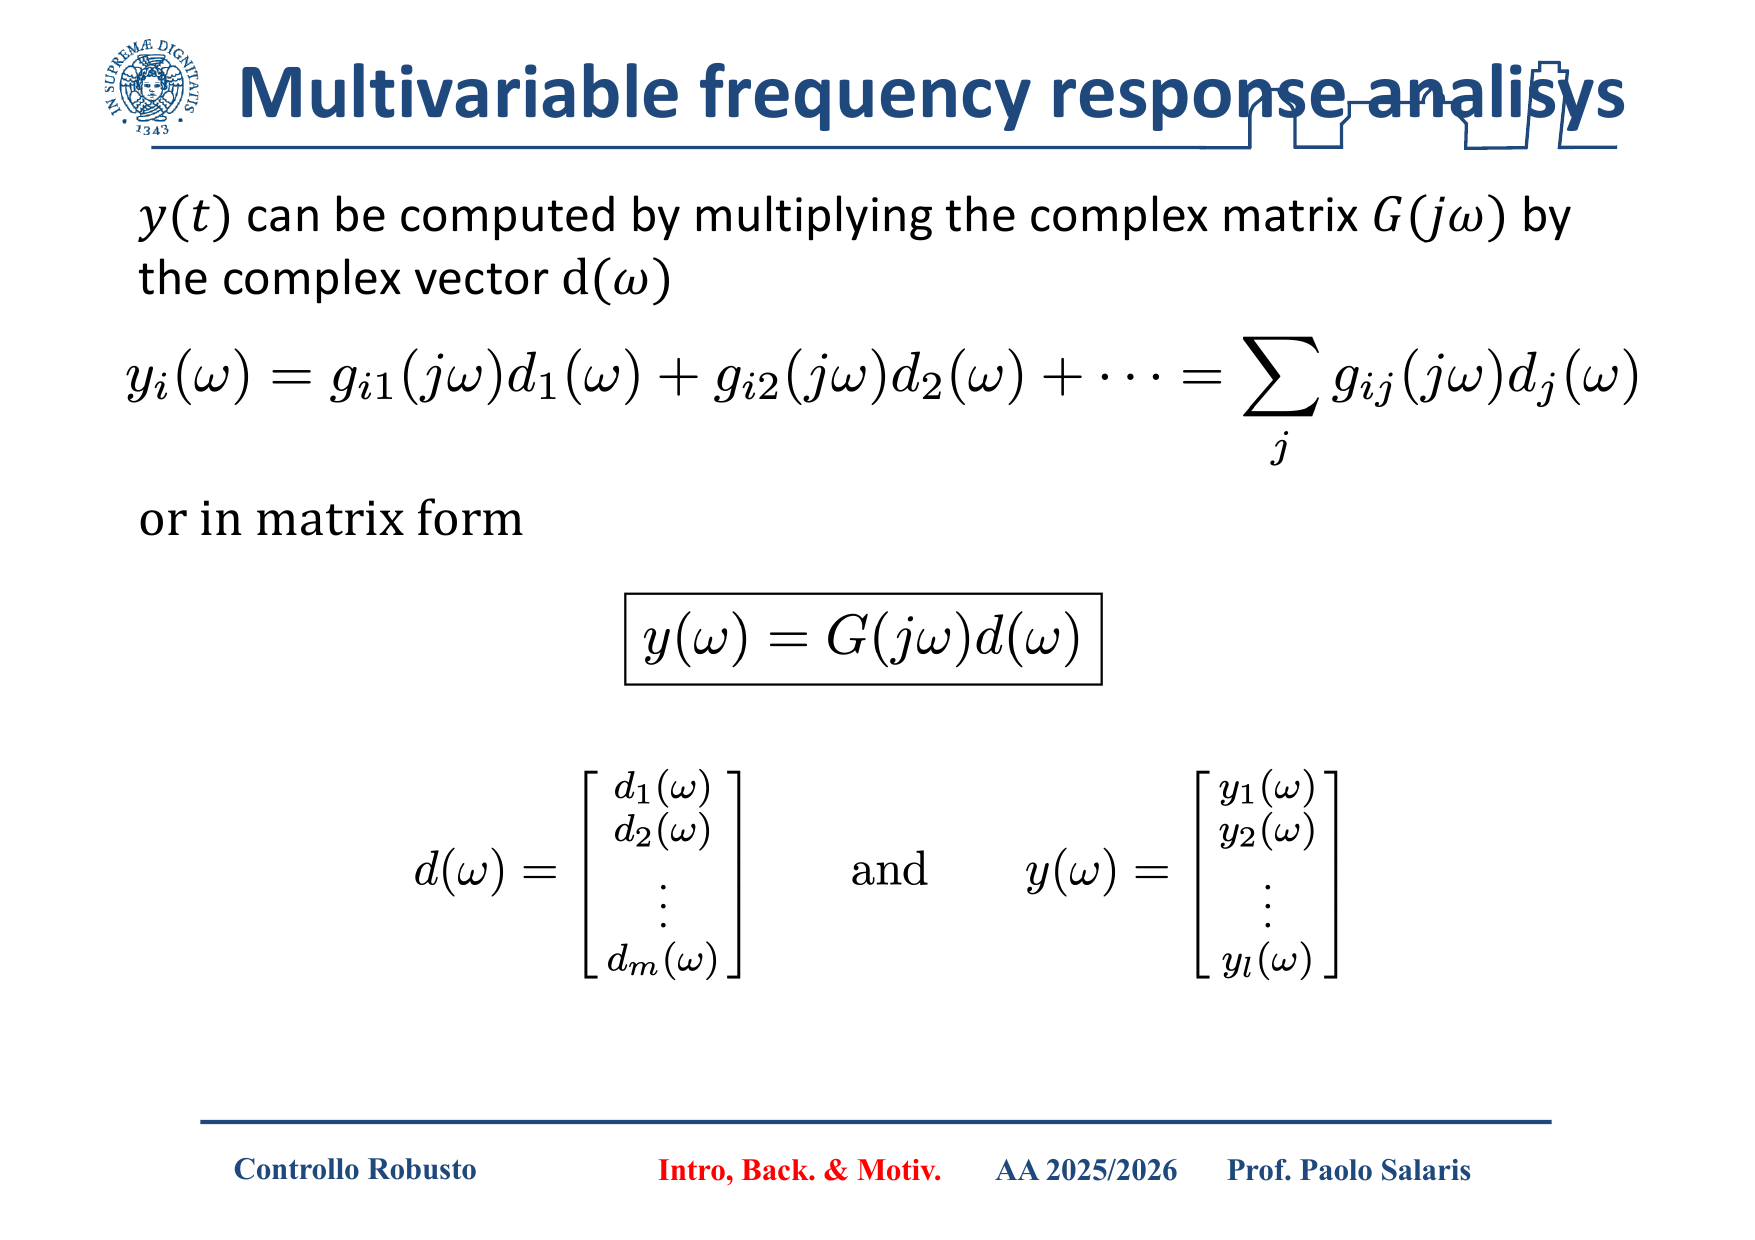
\includegraphics[width=\linewidth]{images3/slide-16.png}
        \caption{La scrittura compatta $y(j\omega)=G(j\omega)d(j\omega)$ mette subito in evidenza il carattere vettoriale del problema.}
    \end{subfigure}
    \hfill
    \begin{subfigure}{0.48\textwidth}
        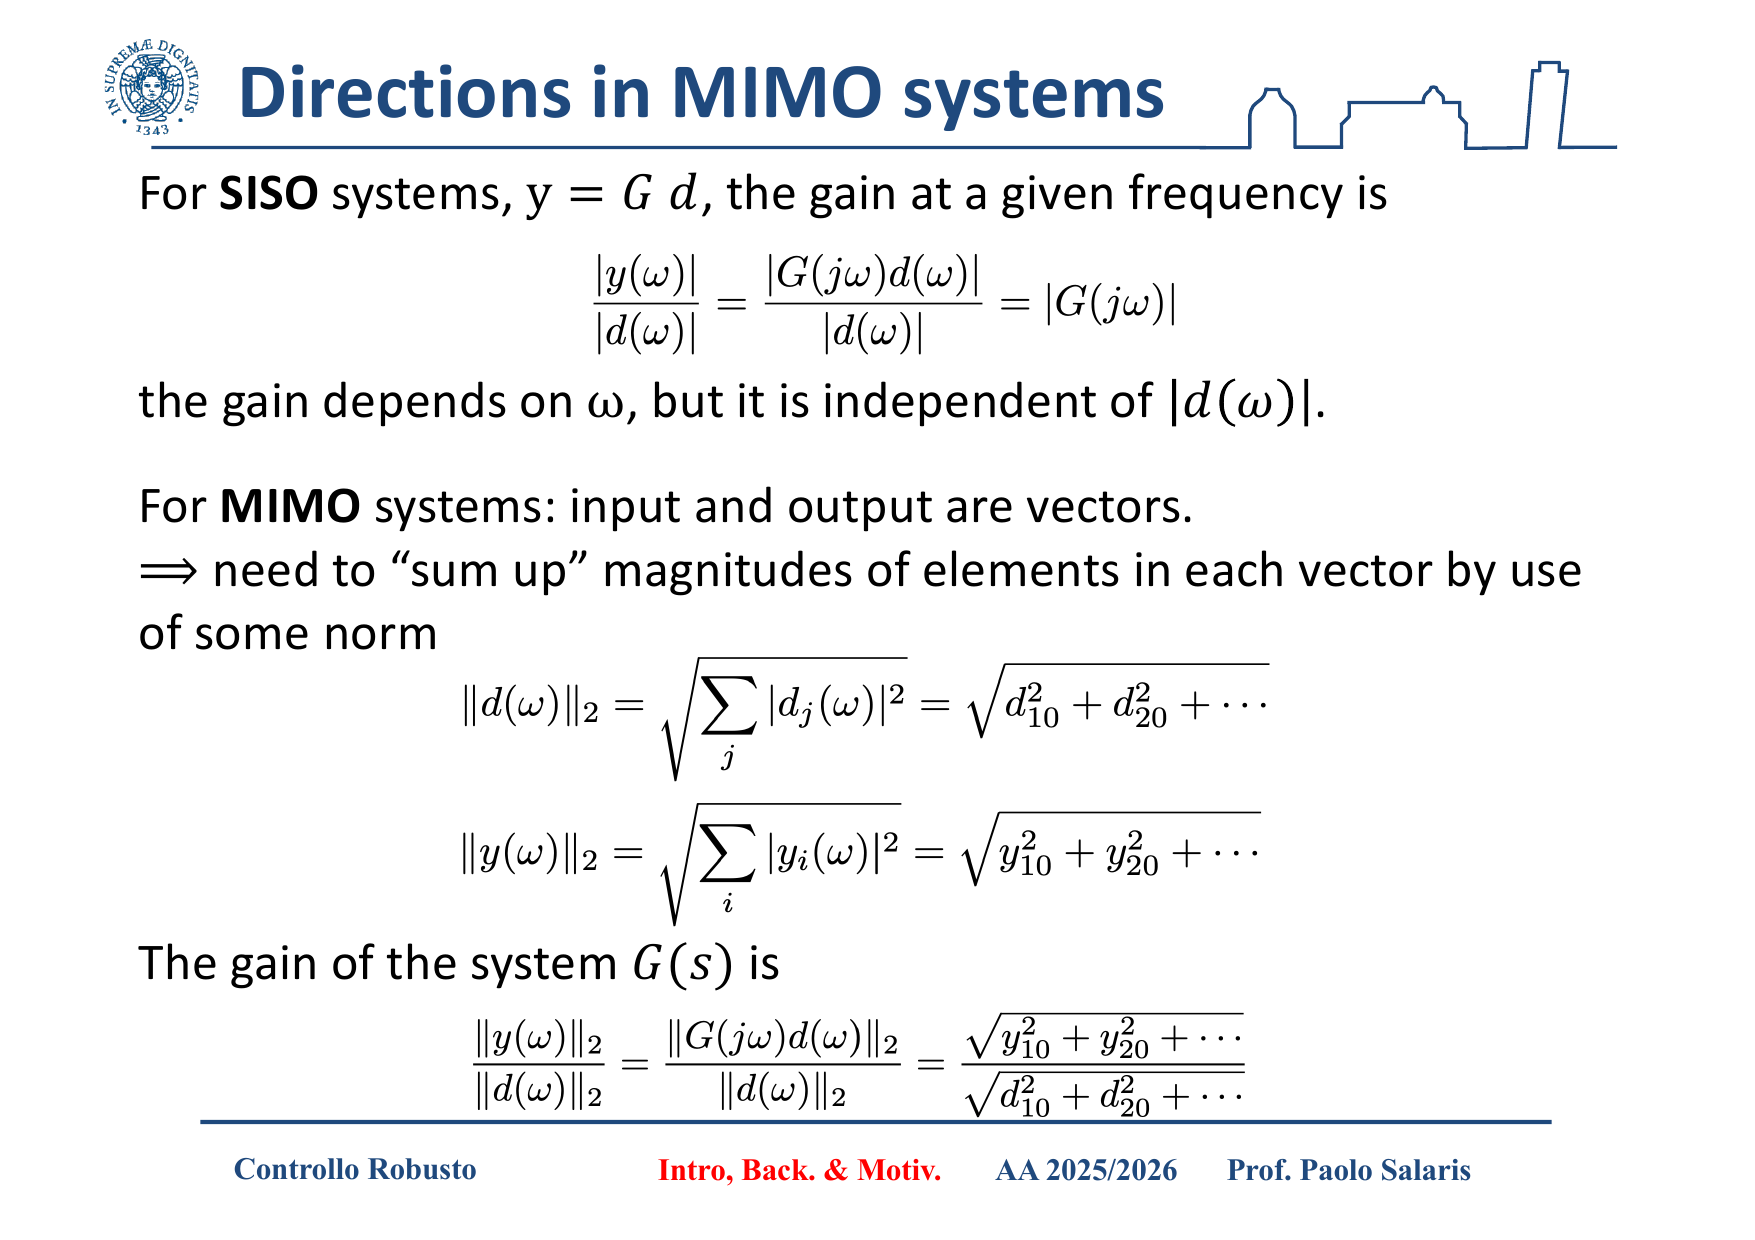
\includegraphics[width=\linewidth]{images3/slide-17.png}
        \caption{Per definire il guadagno occorre introdurre una norma sui vettori di ingresso e di uscita.}
    \end{subfigure}
    \caption{Dal momento in cui input e output sono vettori, la nozione di guadagno deve diventare direzionale.}
\end{figure}

\begin{figure}[H]
    \centering
    \begin{subfigure}{0.48\textwidth}
        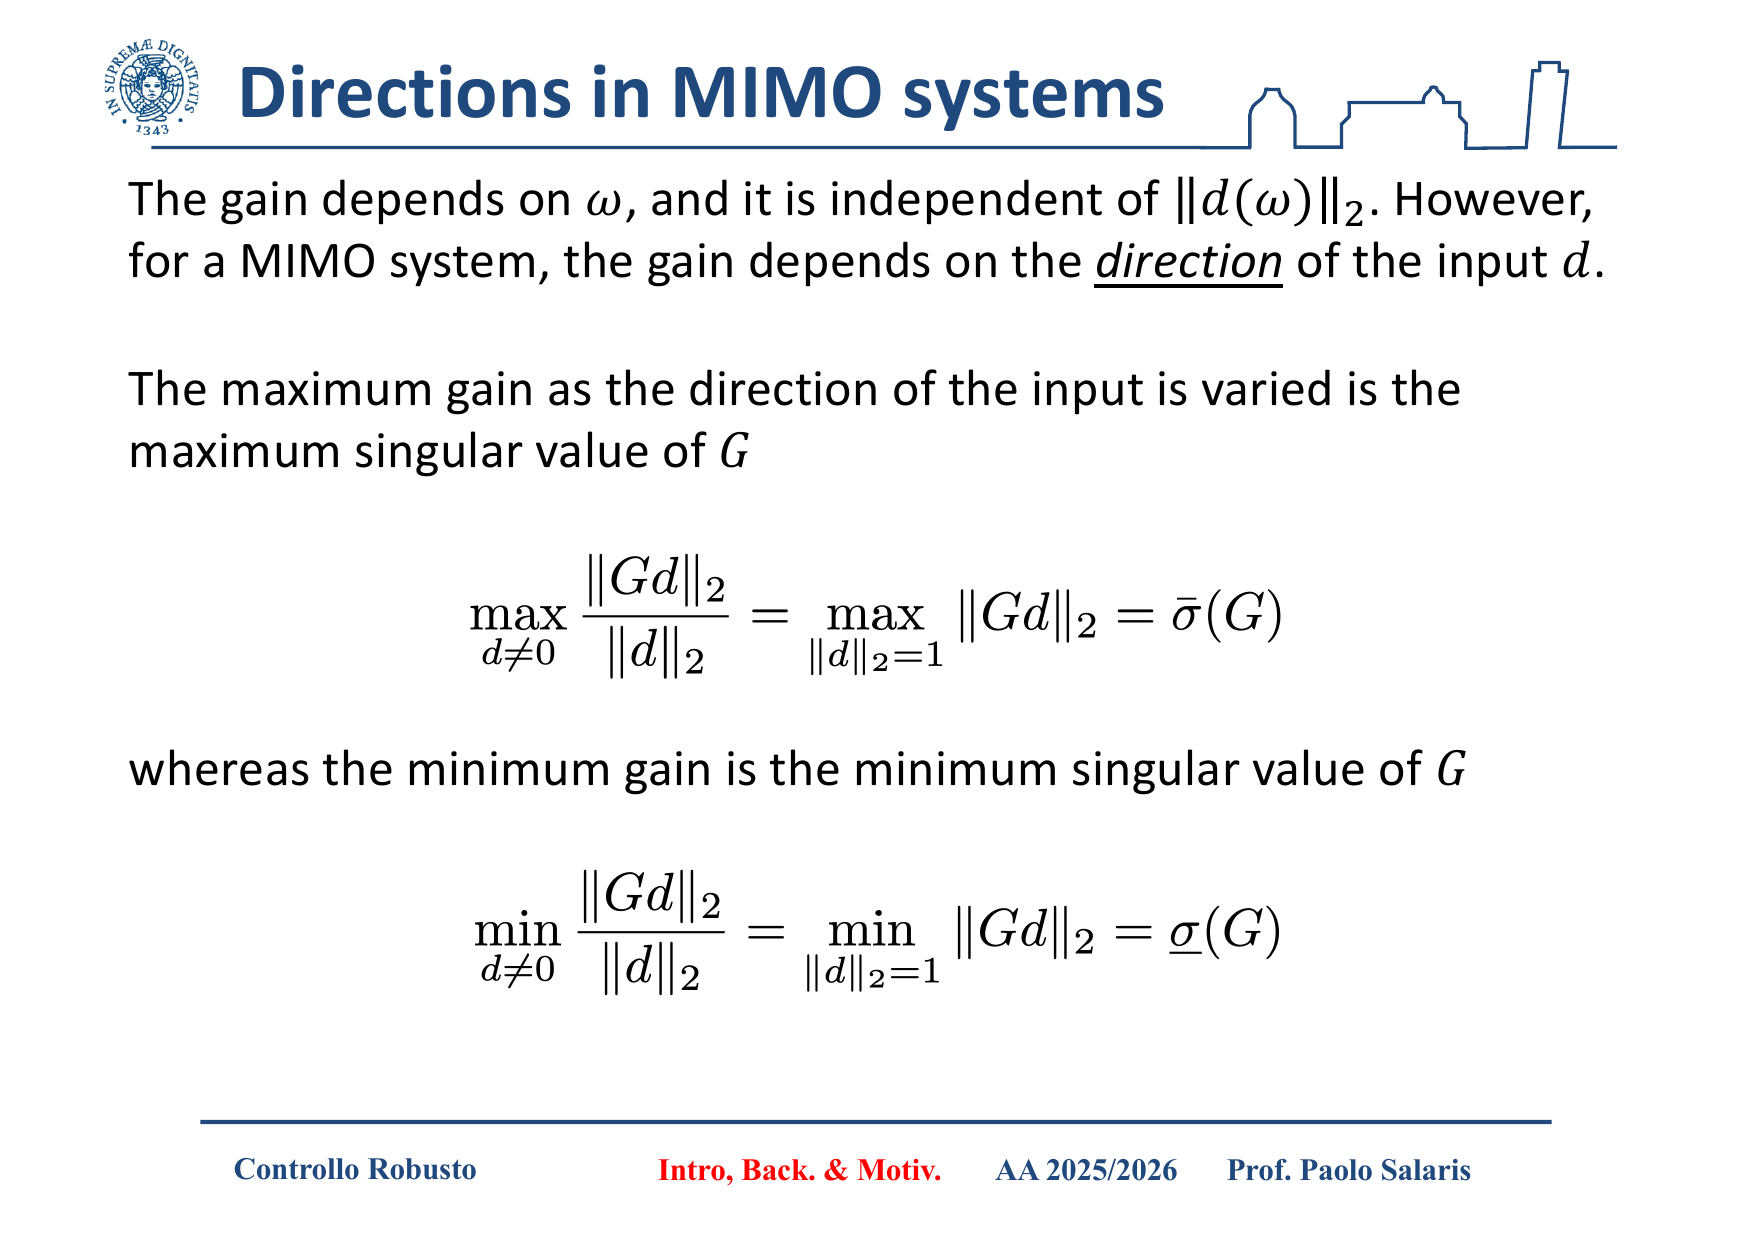
\includegraphics[width=\linewidth]{images3/slide-18.png}
        \caption{Massimo e minimo valore singolare identificano i guadagni estremi del sistema.}
    \end{subfigure}
    \hfill
    \begin{subfigure}{0.48\textwidth}
        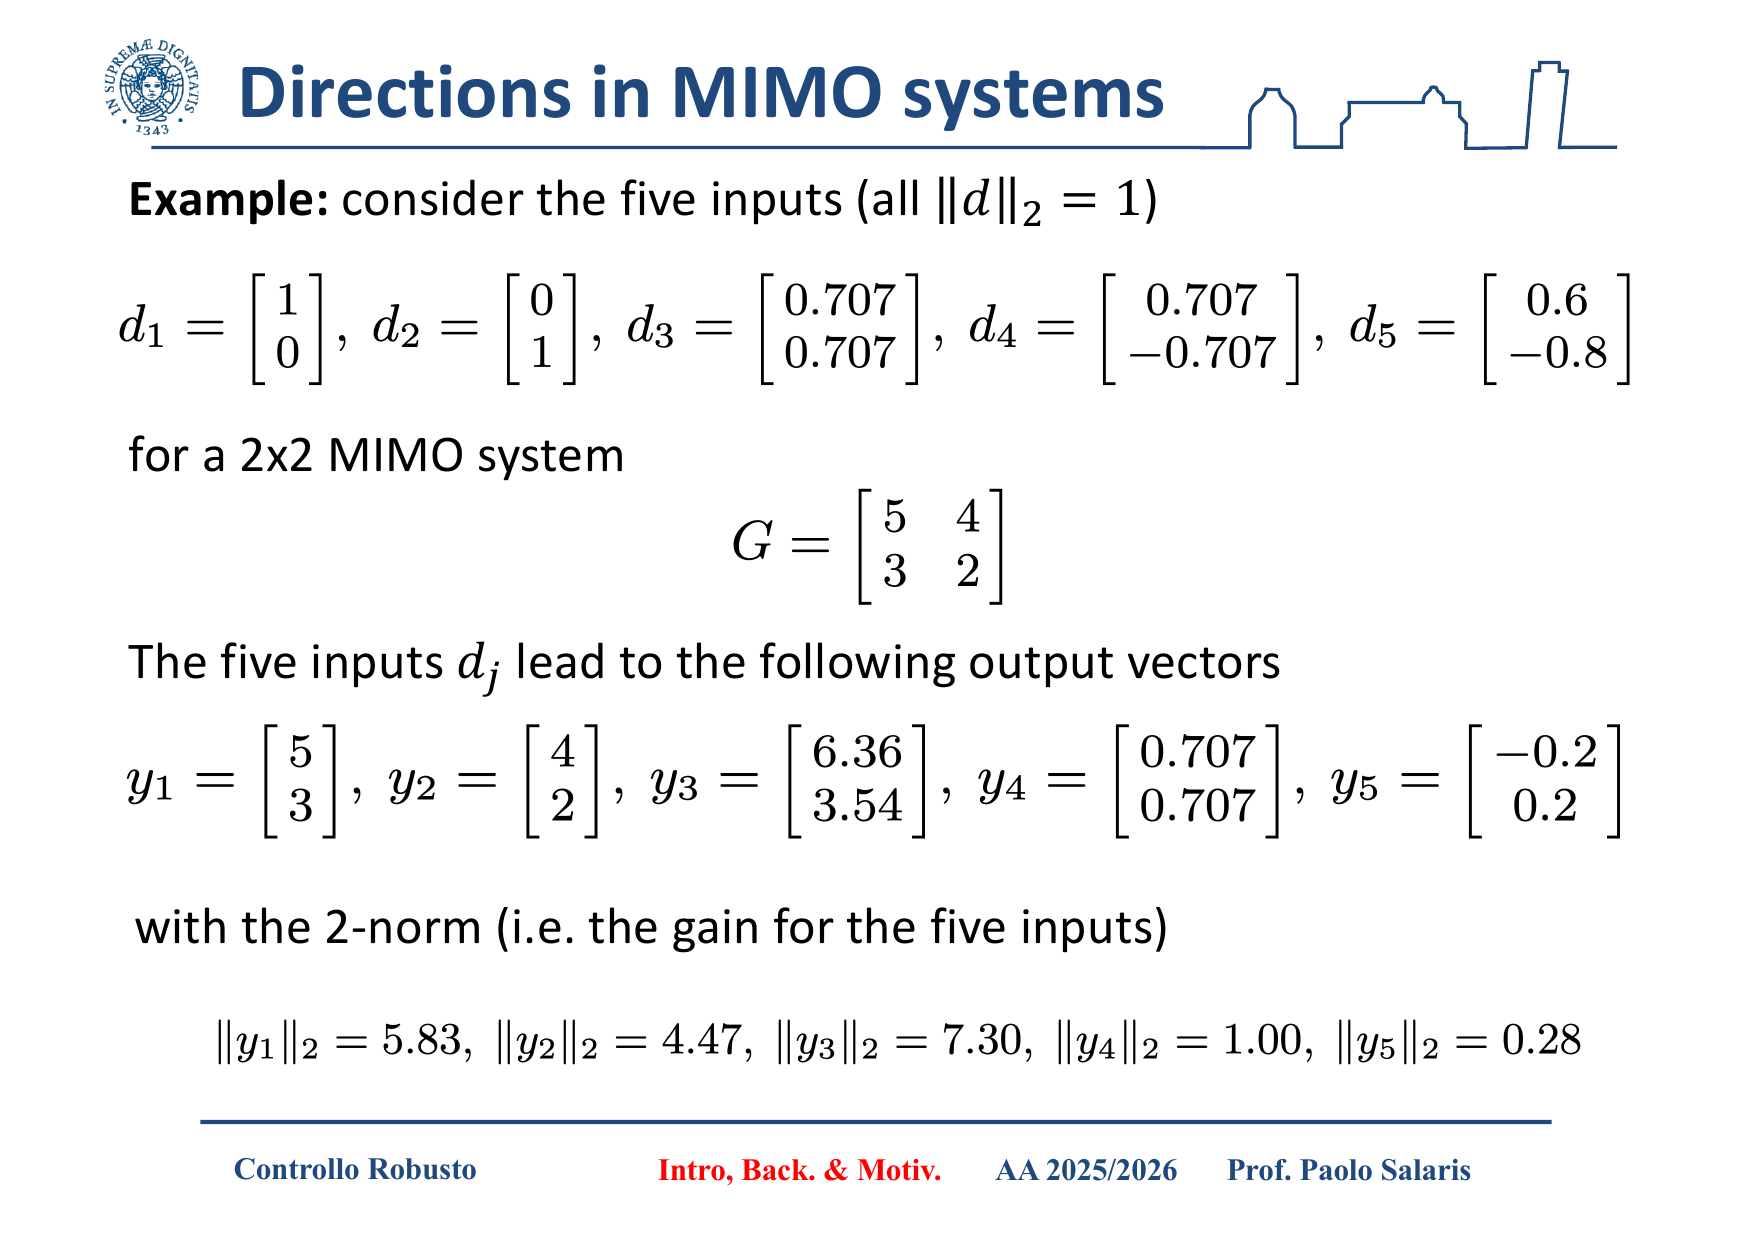
\includegraphics[width=\linewidth]{images3/slide-19.png}
        \caption{Ingressi di uguale norma possono essere amplificati in modo molto diverso a seconda della direzione.}
    \end{subfigure}
    \caption{Le slide 18--19 mostrano che il guadagno MIMO dipende in modo essenziale dalla direzione del vettore di ingresso.}
\end{figure}

\begin{figure}[H]
    \centering
    \begin{subfigure}{0.48\textwidth}
        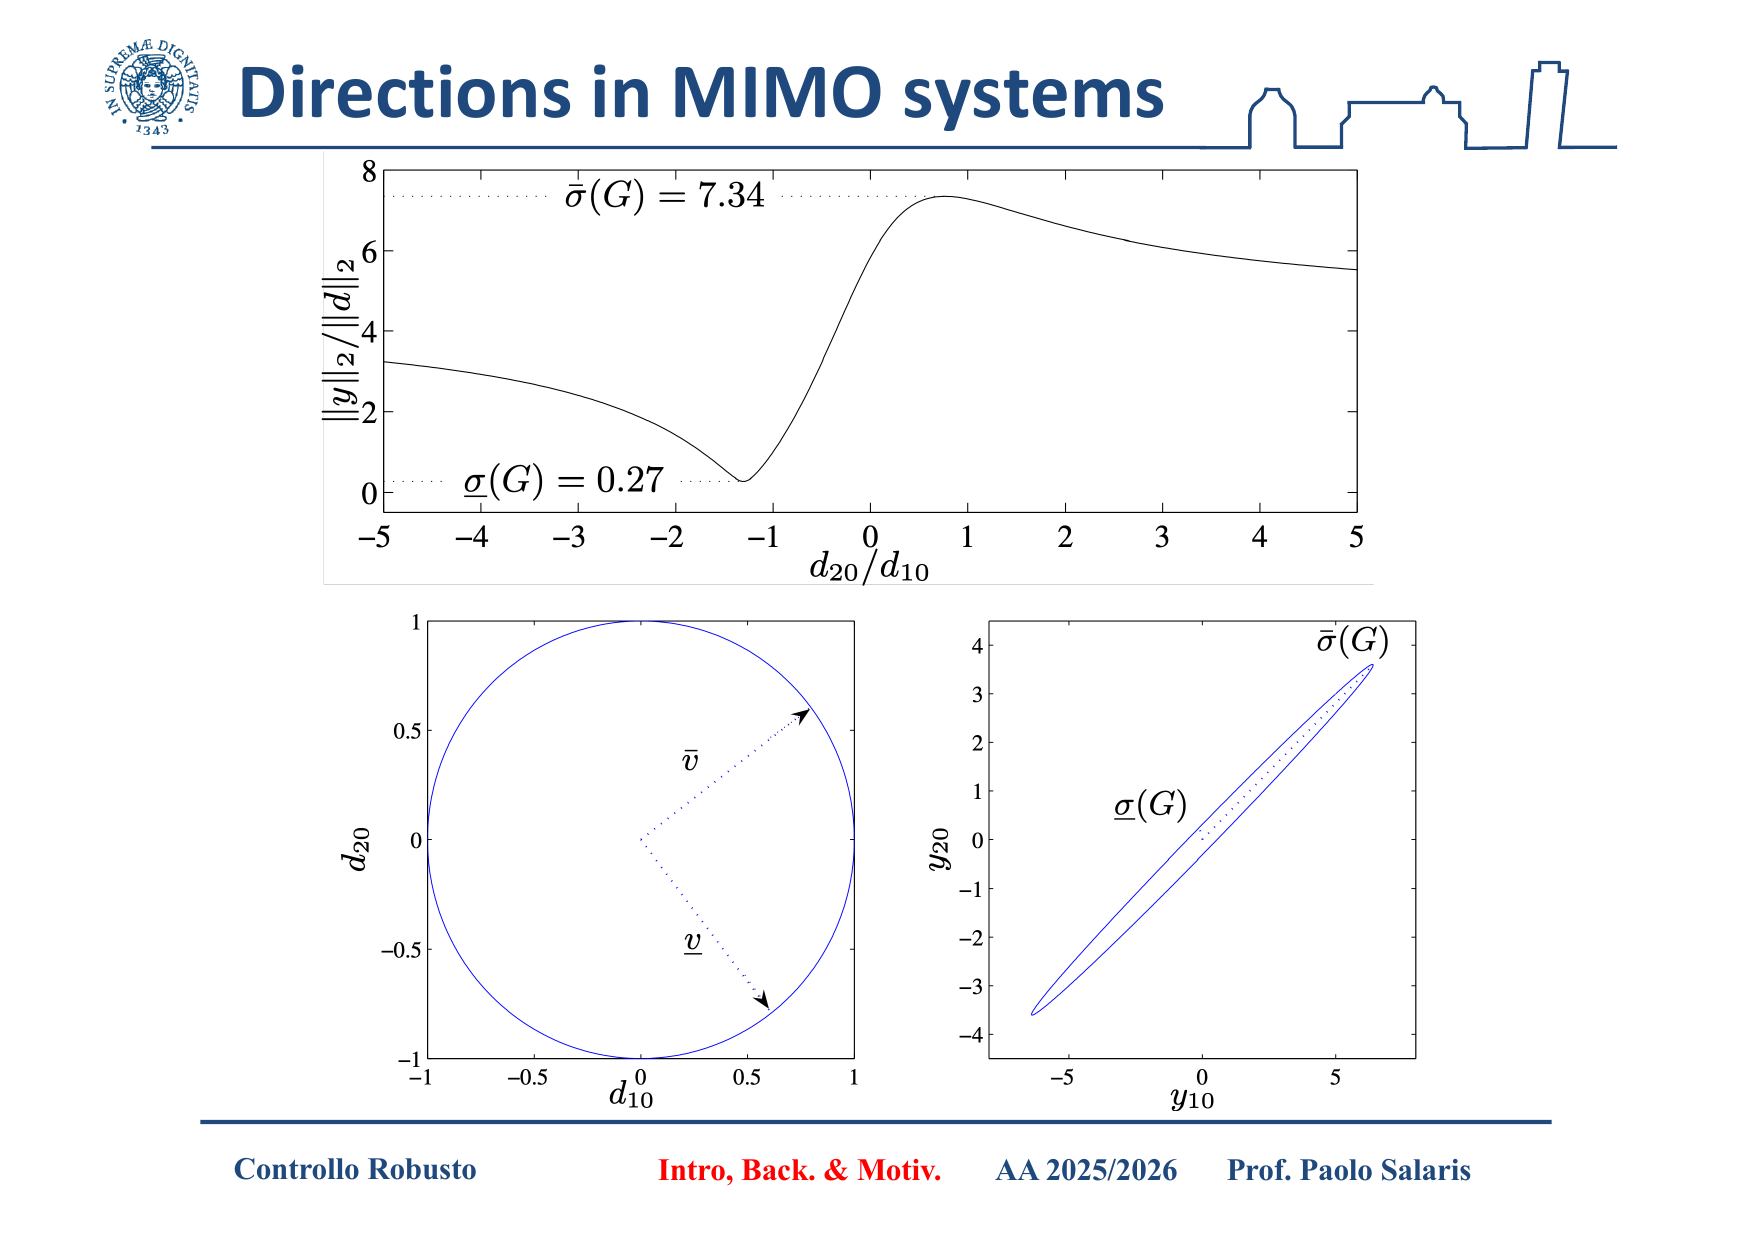
\includegraphics[width=\linewidth]{images3/slide-20.png}
        \caption{La trasformazione della sfera unitaria in un’ellisse visualizza le direzioni forti e deboli.}
    \end{subfigure}
    \hfill
    \begin{subfigure}{0.48\textwidth}
        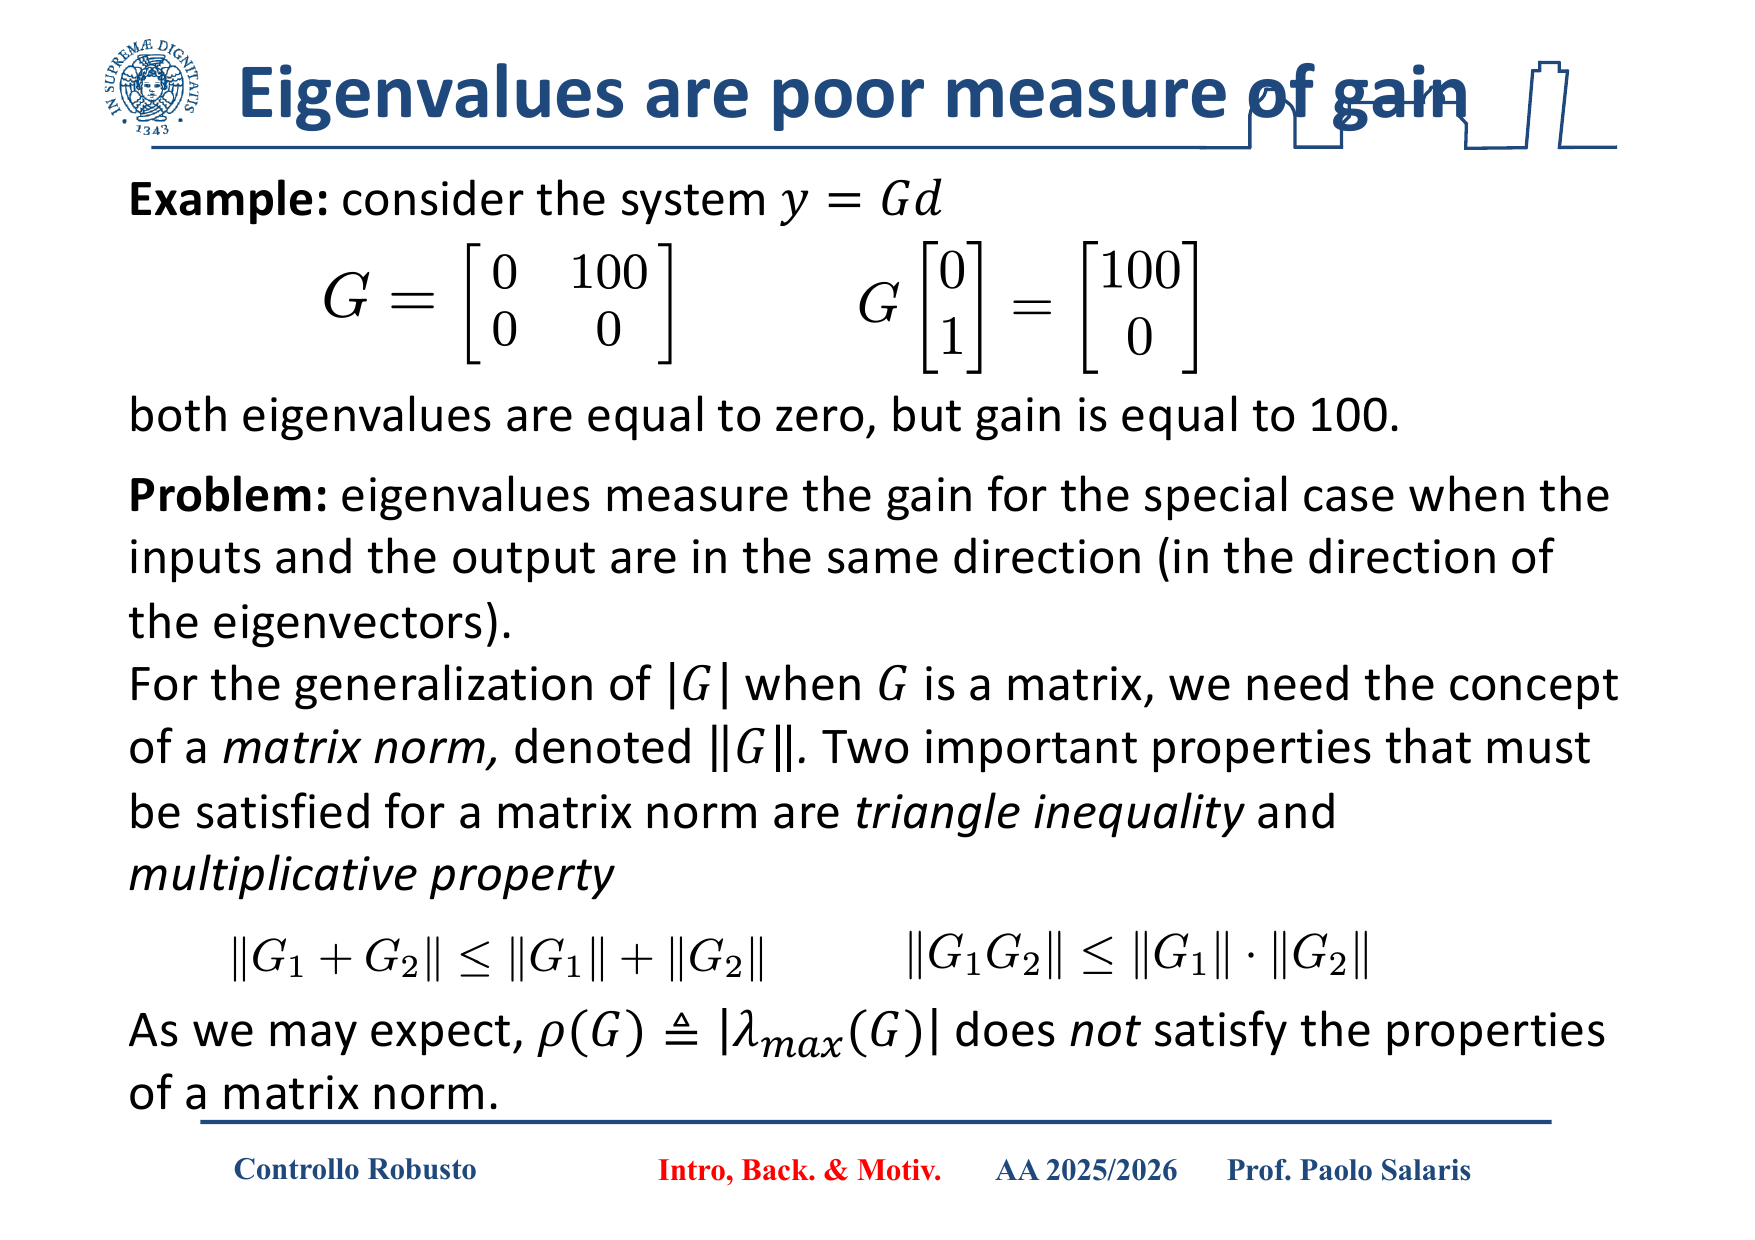
\includegraphics[width=\linewidth]{images3/slide-21.png}
        \caption{Gli autovalori non misurano correttamente il guadagno complessivo della matrice.}
    \end{subfigure}
    \caption{Geometria del guadagno direzionale e limiti di una lettura basata soltanto sugli autovalori.}
\end{figure}

\subsection{Guadagni principali, SVD e significato dei loci caratteristici}

Prima di introdurre formalmente la SVD, la lezione chiarisce un punto spesso sottovalutato: il vecchio linguaggio dei \emph{characteristic loci} resta utile solo in un caso speciale, quello delle matrici normali. Se una matrice quadrata $Q$ soddisfa
$$
Q^\ast Q = QQ^\ast,
$$
allora i suoi autovettori formano una base ortogonale e i valori singolari coincidono con i moduli degli autovalori:
$$
\sigma_i(Q)=|\lambda_i(Q)|.
$$
In questo caso i loci caratteristici, cioè le traiettorie degli autovalori nel dominio della frequenza, forniscono anche un’informazione diretta sui guadagni principali.

Il punto importante, però, è proprio il contrario: \emph{fuori} dalla classe delle matrici normali questa coincidenza si perde. Gli autovalori continuano a descrivere alcune proprietà spettrali del sistema, ma non rappresentano più i guadagni effettivi nelle direzioni rilevanti. Ecco perché la teoria moderna del controllo robusto passa dai loci caratteristici ai \emph{principal gains}, cioè ai valori singolari.

La decomposizione ai valori singolari fornisce allora la struttura giusta:
$$
G(j\omega)=U(j\omega)\,\Sigma(j\omega)\,V(j\omega)^\ast.
$$
Le colonne di $V$ sono le direzioni principali di ingresso, le colonne di $U$ sono le direzioni principali di uscita, mentre la diagonale di $\Sigma$ contiene i valori singolari ordinati in modo decrescente. La relazione
$$
Gv_i=\sigma_i u_i
$$
ha un significato fisico immediato: eccitare il sistema lungo la direzione $v_i$ produce un’uscita allineata con $u_i$ e amplificata di un fattore $\sigma_i$.

Questo è esattamente il linguaggio che servirà nella Lezione 5. Quando si richiederà che certi canali chiusi abbiano massimo valore singolare piccolo o che il loop gain abbia minimo valore singolare grande in una certa banda, si starà semplicemente usando la SVD per trasformare nozioni qualitative di prestazione e robustezza in condizioni quantitative leggibili in tutte le direzioni rilevanti.

\begin{figure}[H]
    \centering
    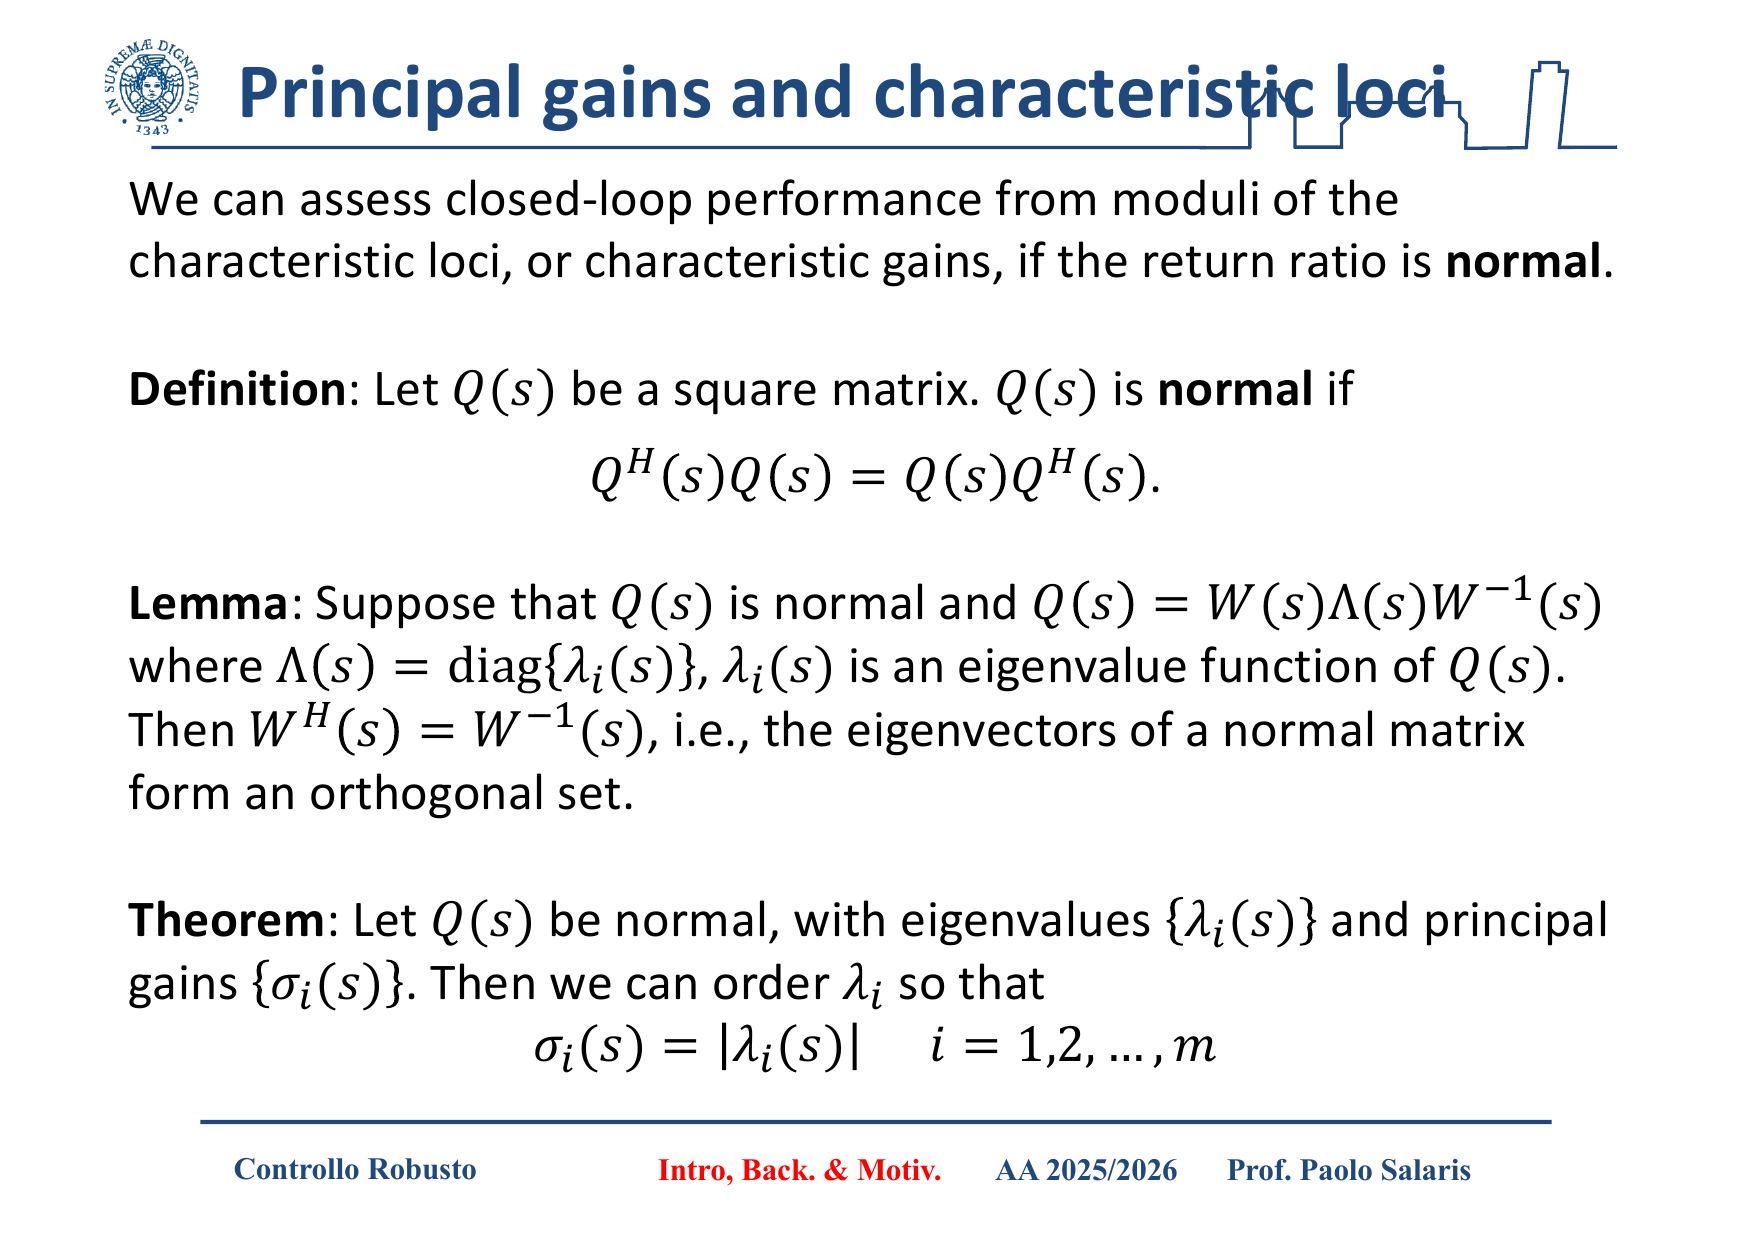
\includegraphics[width=0.8\textwidth]{images3/slide-22.png}
    \caption{Nel caso di matrici normali i loci caratteristici e i guadagni principali coincidono, ma questa è un’eccezione e non la regola generale.}
\end{figure}

\begin{figure}[H]
    \centering
    \begin{subfigure}{0.32\textwidth}
        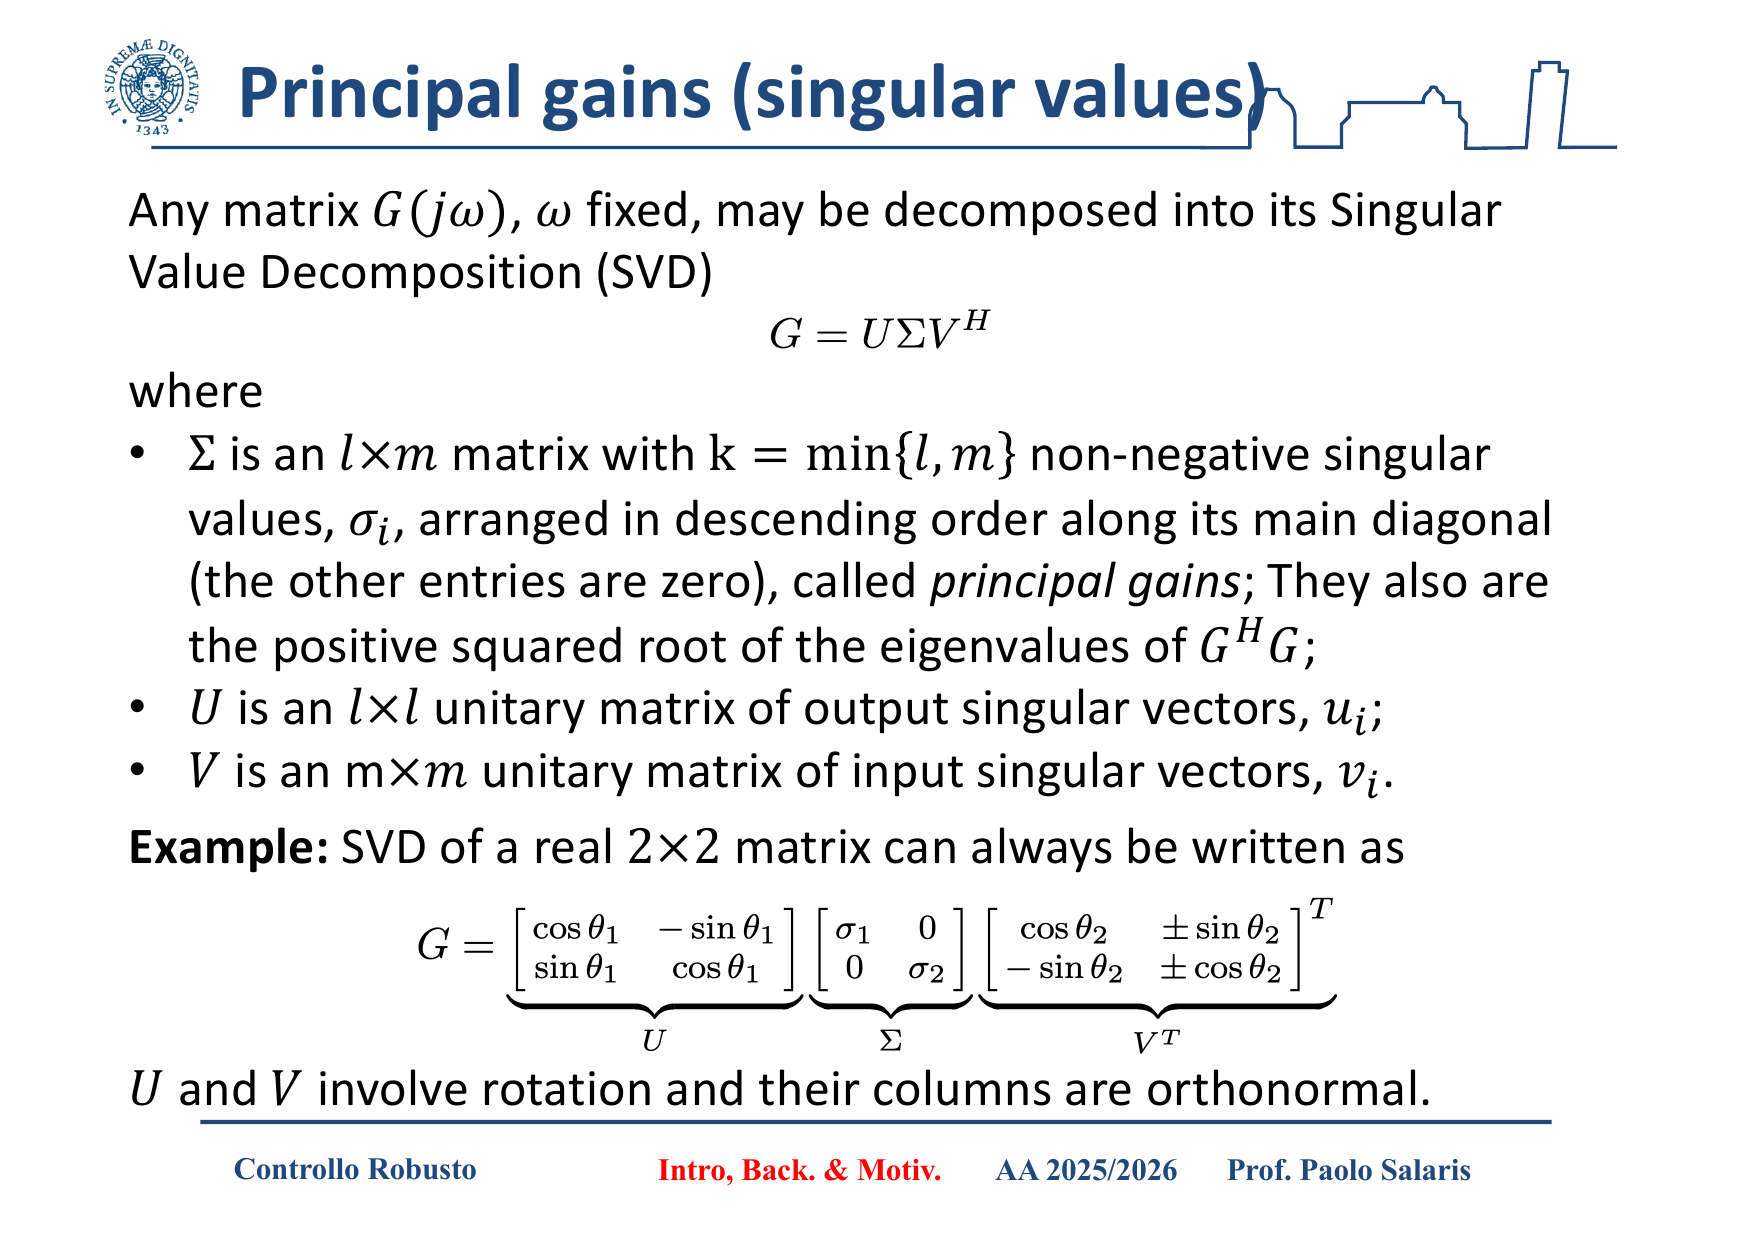
\includegraphics[width=\linewidth]{images3/slide-23.png}
        \caption{La SVD separa direzioni di ingresso, direzioni di uscita e guadagni associati.}
    \end{subfigure}
    \hfill
    \begin{subfigure}{0.32\textwidth}
        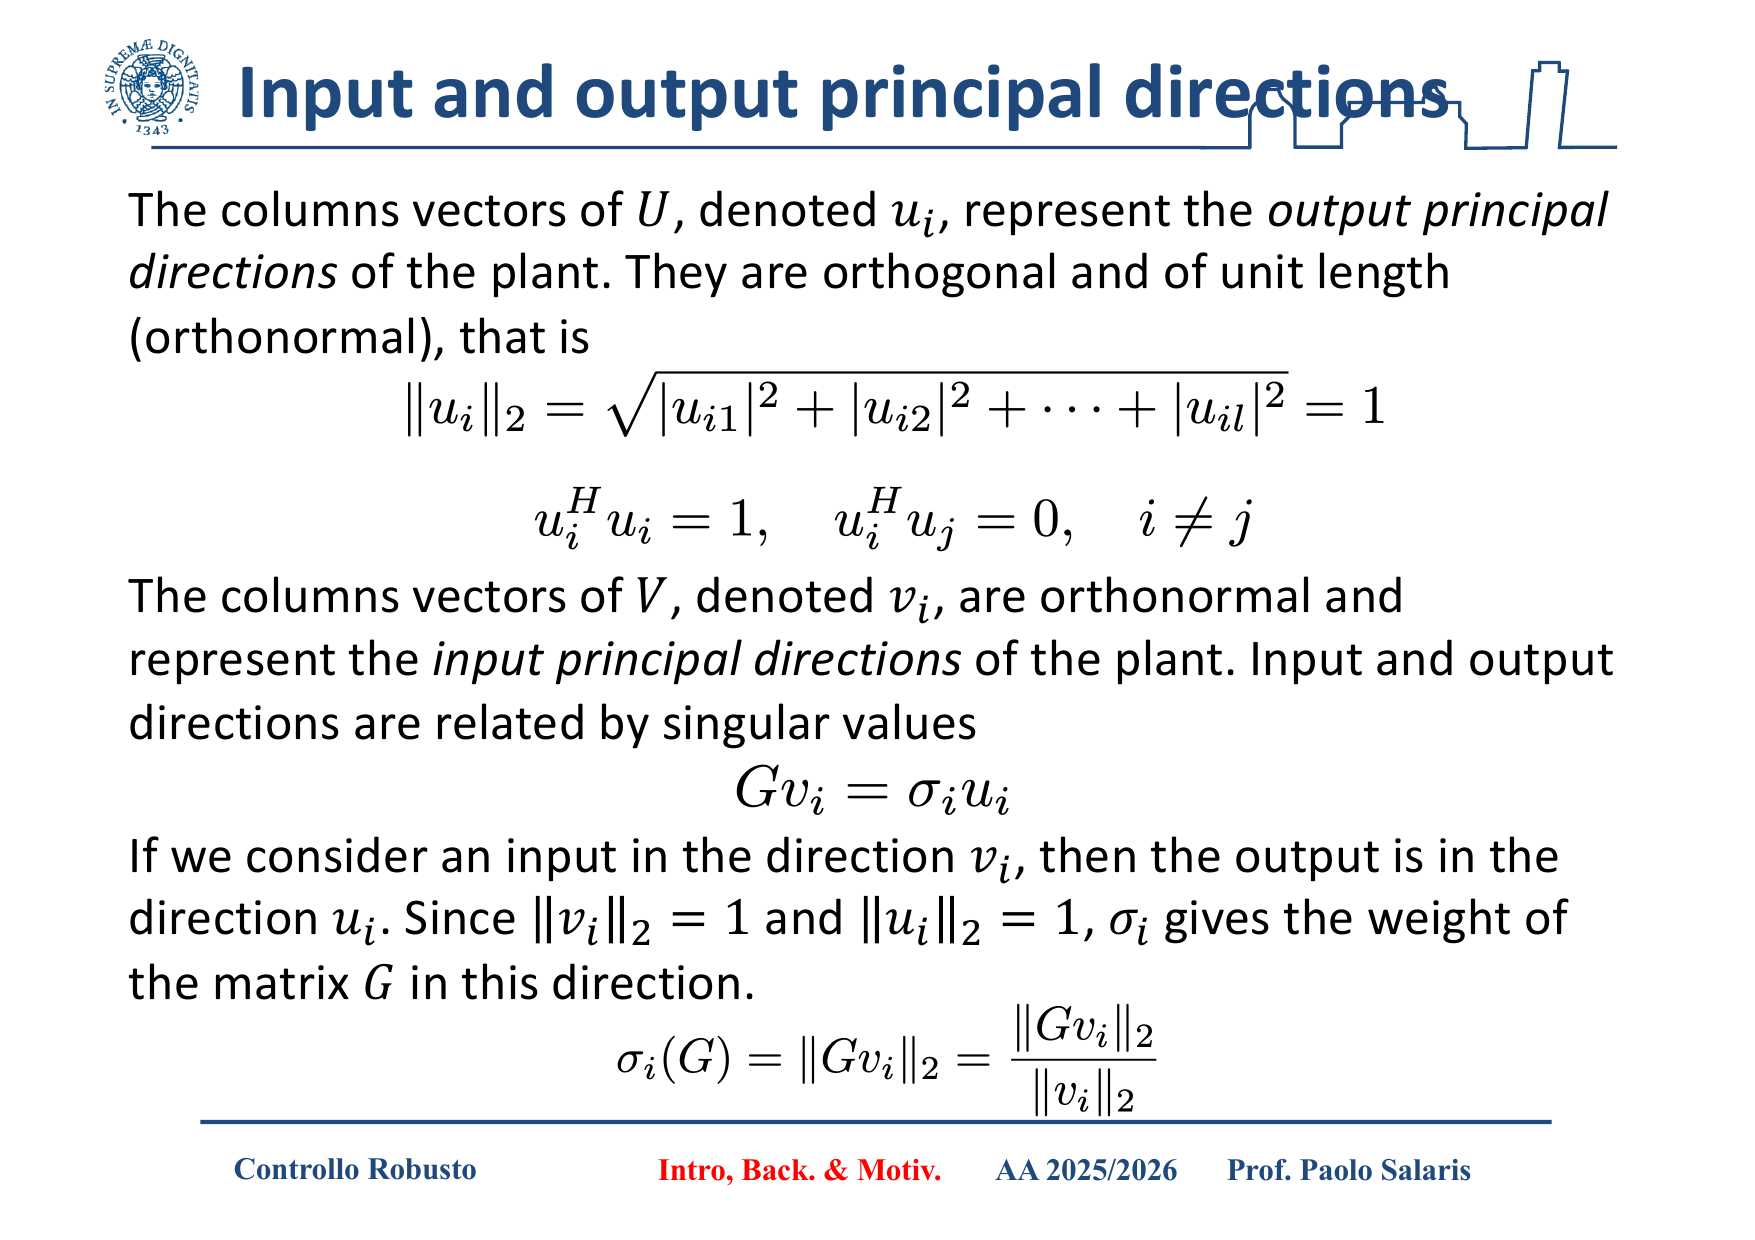
\includegraphics[width=\linewidth]{images3/slide-24.png}
        \caption{Le direzioni principali descrivono come il sistema ruota e amplifica i vettori di ingresso.}
    \end{subfigure}
    \hfill
    \begin{subfigure}{0.32\textwidth}
        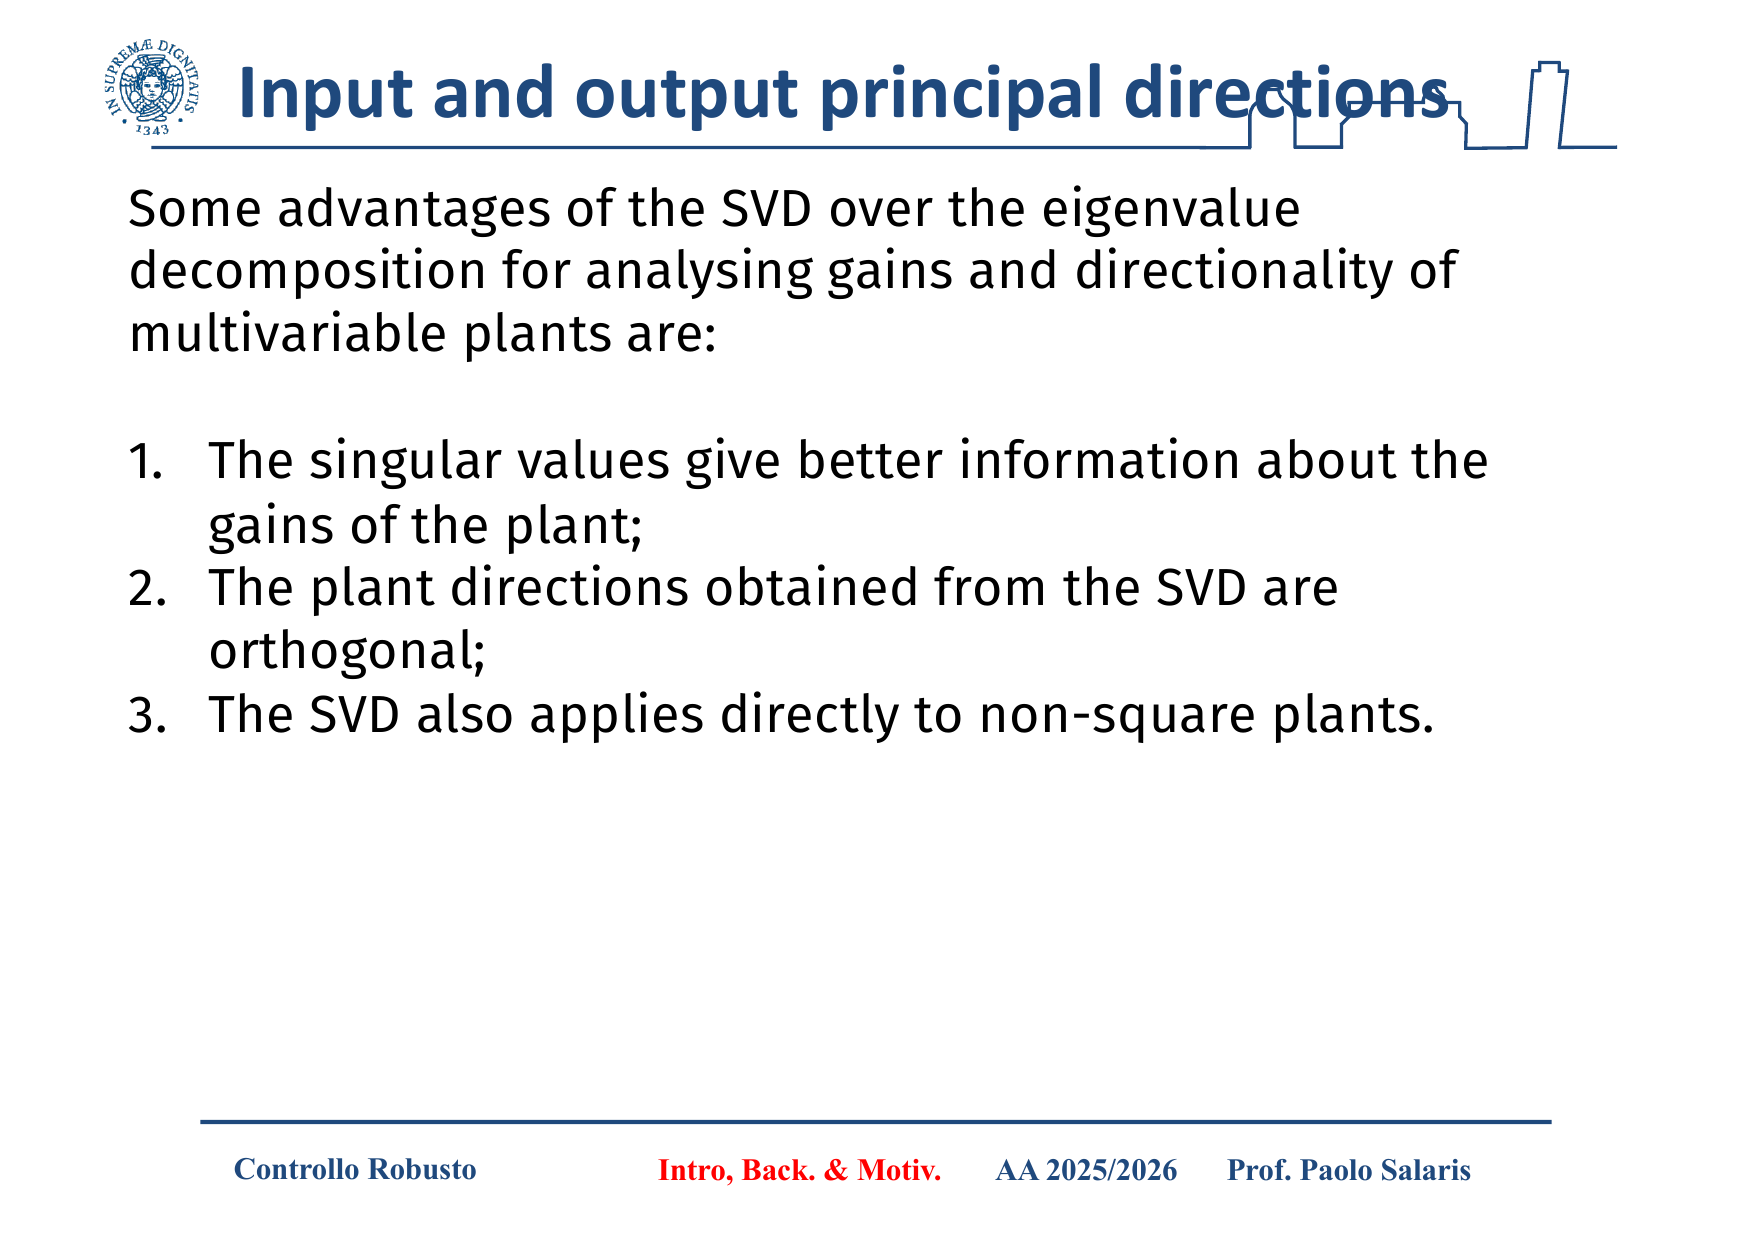
\includegraphics[width=\linewidth]{images3/slide-25.png}
        \caption{I valori singolari forniscono informazioni più robuste degli autovalori e valgono anche per impianti non quadrati.}
    \end{subfigure}
    \caption{La SVD diventa lo strumento naturale per leggere guadagni e direzioni nei sistemi multivariabili.}
\end{figure}

\subsection{Mal condizionamento e significato fisico delle direzioni singolari}

L’ultimo blocco della lezione porta la SVD dal piano formale a quello fisico. Il massimo e il minimo valore singolare delimitano l’intervallo di guadagno che il sistema può realizzare alla frequenza considerata. Le direzioni associate a $\bar{\sigma}(G)$ sono le direzioni forti: piccole azioni lungo tali combinazioni di ingresso producono effetti molto marcati in uscita. Le direzioni associate a $\underline{\sigma}(G)$ sono invece le direzioni deboli: in esse il processo reagisce poco, per cui ottenere la stessa variazione di uscita richiede molta più azione di controllo.

Da qui nasce il \emph{numero di condizionamento}
$$
\kappa(G)=\frac{\bar{\sigma}(G)}{\underline{\sigma}(G)}.
$$
Quando $\kappa(G)$ è vicino a $1$, il guadagno del sistema è relativamente isotropo: nessuna direzione è troppo favorita o troppo penalizzata. Quando invece $\kappa(G)$ è grande, il processo è mal condizionato. In questo caso il controllore deve confrontarsi con un problema fortemente sbilanciato: alcune combinazioni di ingressi sono facilissime da influenzare, altre restano quasi inerti. Dal punto di vista del controllo robusto, questo significa che una sintesi efficace in una direzione può convivere con prestazioni molto deboli in un’altra.

Gli esempi finali delle slide servono proprio a rendere visibile questa idea. L’analogia della carriola con ruote fisse mostra che non tutte le direzioni di movimento hanno la stessa ``facilità'': andare avanti è naturale, spostarsi lateralmente lo è molto meno. Il processo di distillazione mostra la stessa cosa in un contesto ingegneristico reale. Guardando soltanto i singoli coefficienti della matrice statica si potrebbe concludere che il processo abbia guadagni grandi e quindi sia semplice da controllare. La SVD rivela invece una struttura molto più sottile: esiste una direzione ad altissimo guadagno e una direzione molto più debole, legata al fatto che in certe combinazioni i due ingressi tendono a contrastarsi reciprocamente.

Questa conclusione è estremamente importante anche per lo studio. Nei sistemi multivariabili non basta più leggere una matrice ``voce per voce'' e non basta guardare il segno o il modulo dei singoli elementi. Il comportamento davvero rilevante è quello delle combinazioni lineari di attuatori e uscite selezionate dai vettori singolari. Per questo le ultime slide non sono un’appendice matematica, ma il punto in cui la risposta in frequenza MIMO diventa davvero interpretabile dal punto di vista fisico.

\begin{figure}[H]
    \centering
    \begin{subfigure}{0.32\textwidth}
        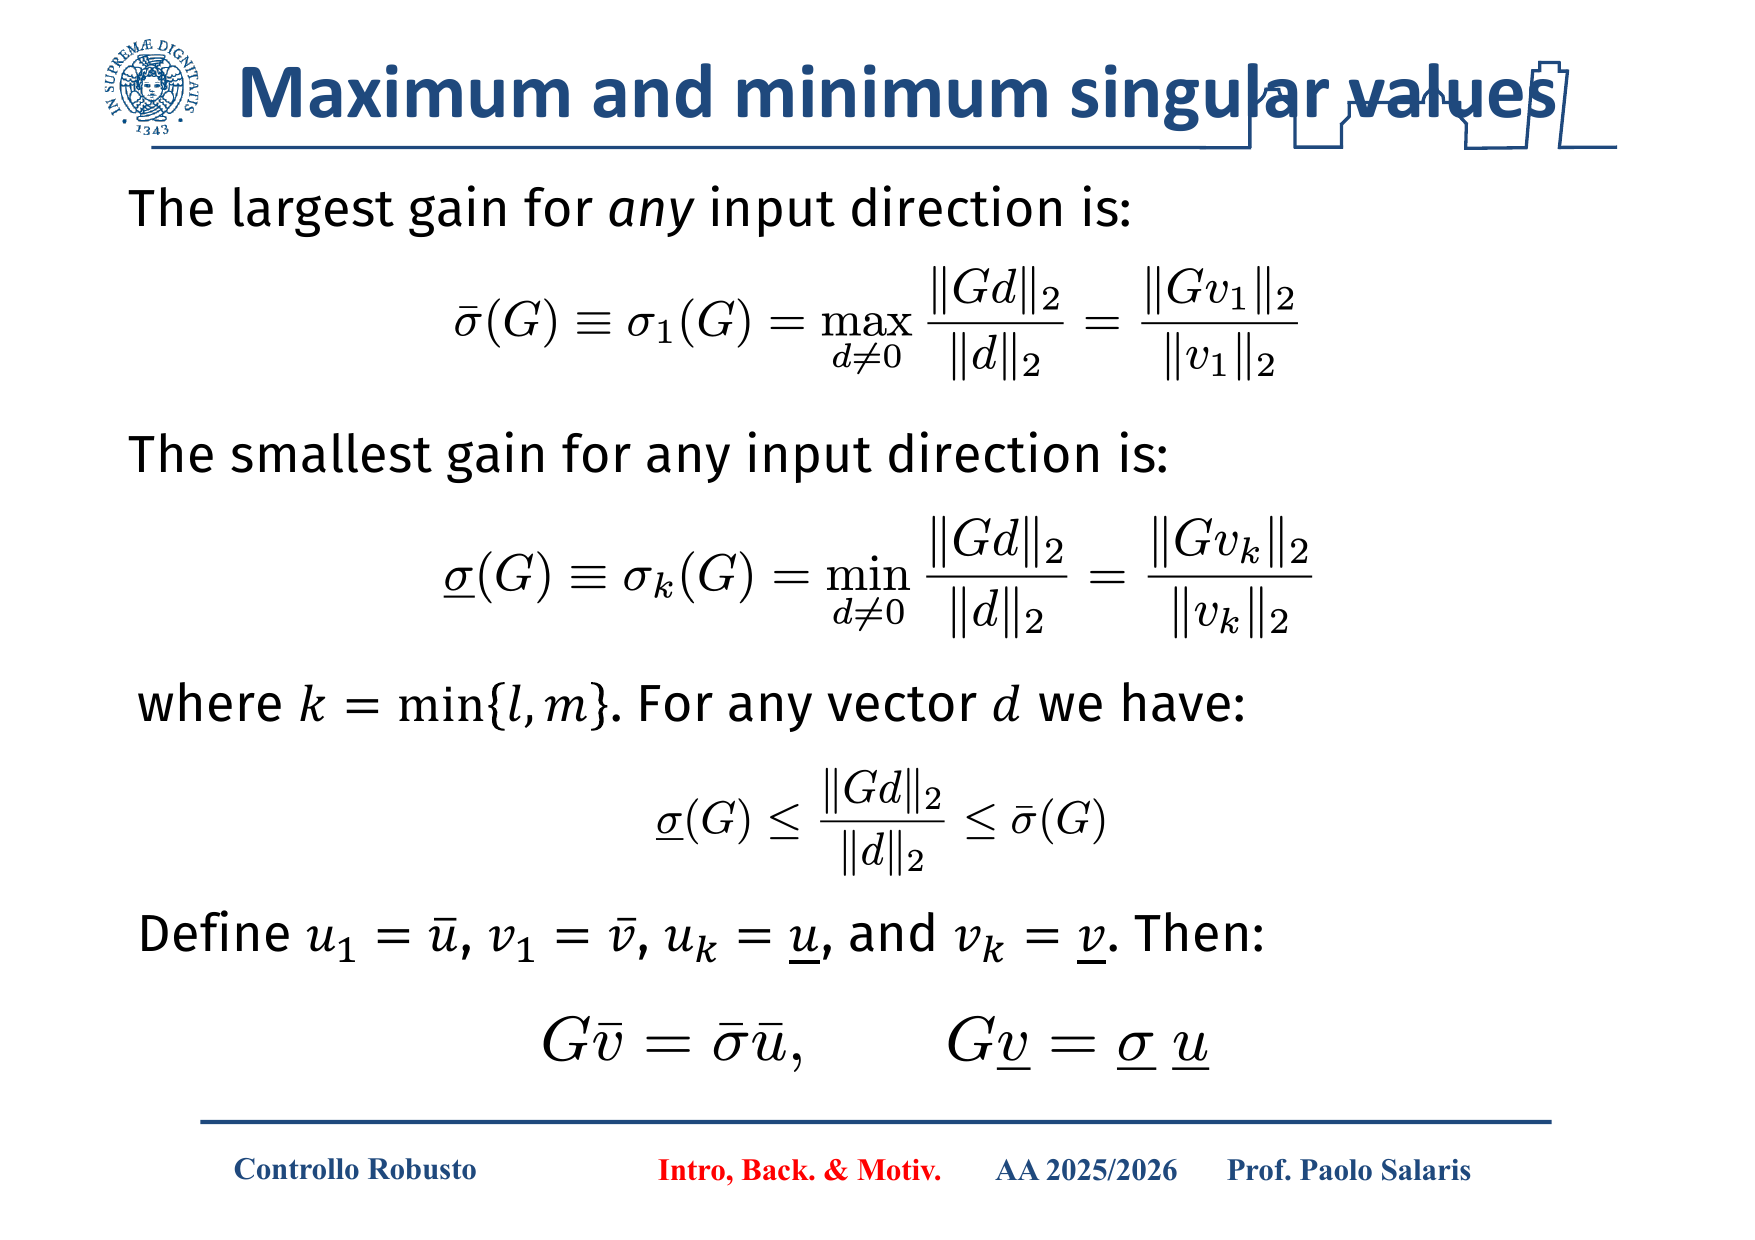
\includegraphics[width=\linewidth]{images3/slide-26.png}
        \caption{Il massimo e il minimo valore singolare delimitano l’intervallo di guadagni ottenibili.}
    \end{subfigure}
    \hfill
    \begin{subfigure}{0.32\textwidth}
        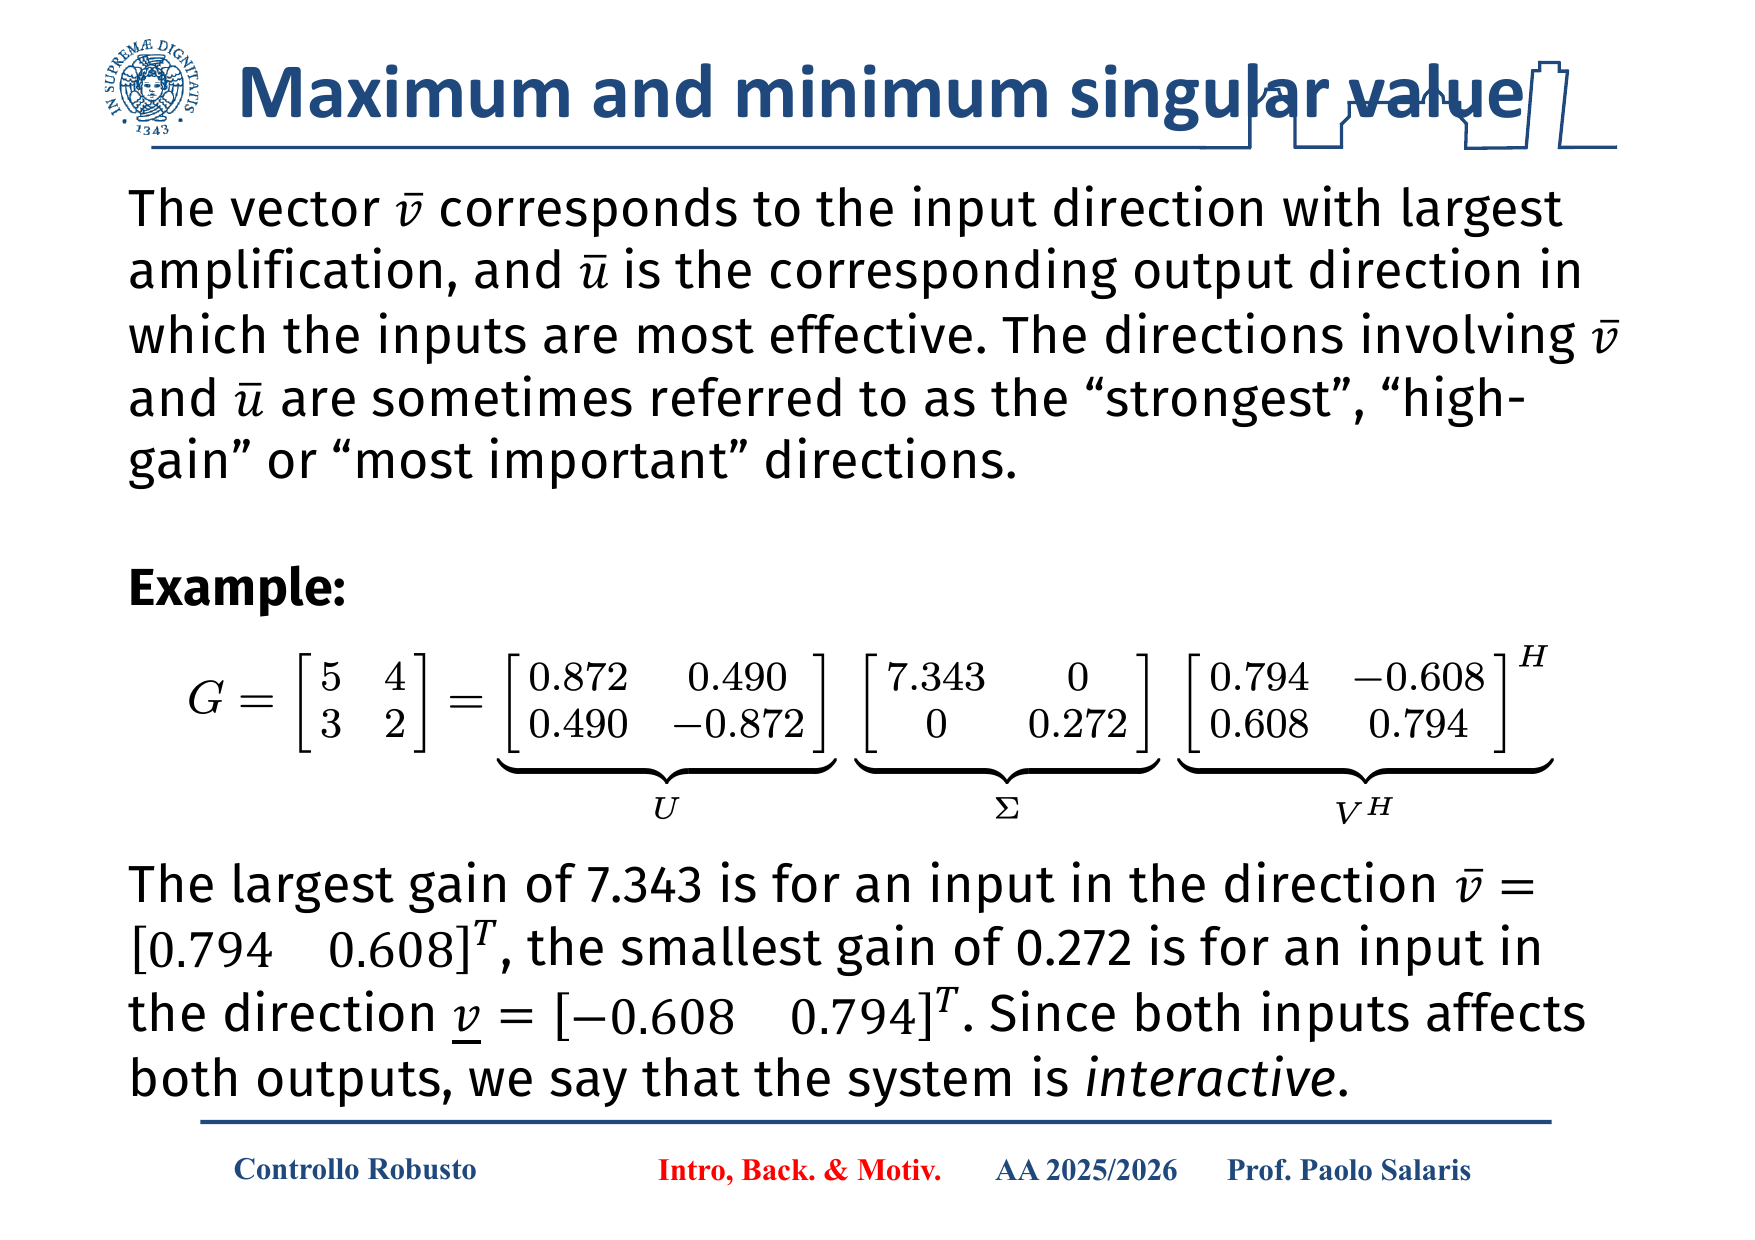
\includegraphics[width=\linewidth]{images3/slide-27.png}
        \caption{Le direzioni corrispondenti identificano i canali più forti e quelli più deboli del processo.}
    \end{subfigure}
    \hfill
    \begin{subfigure}{0.32\textwidth}
        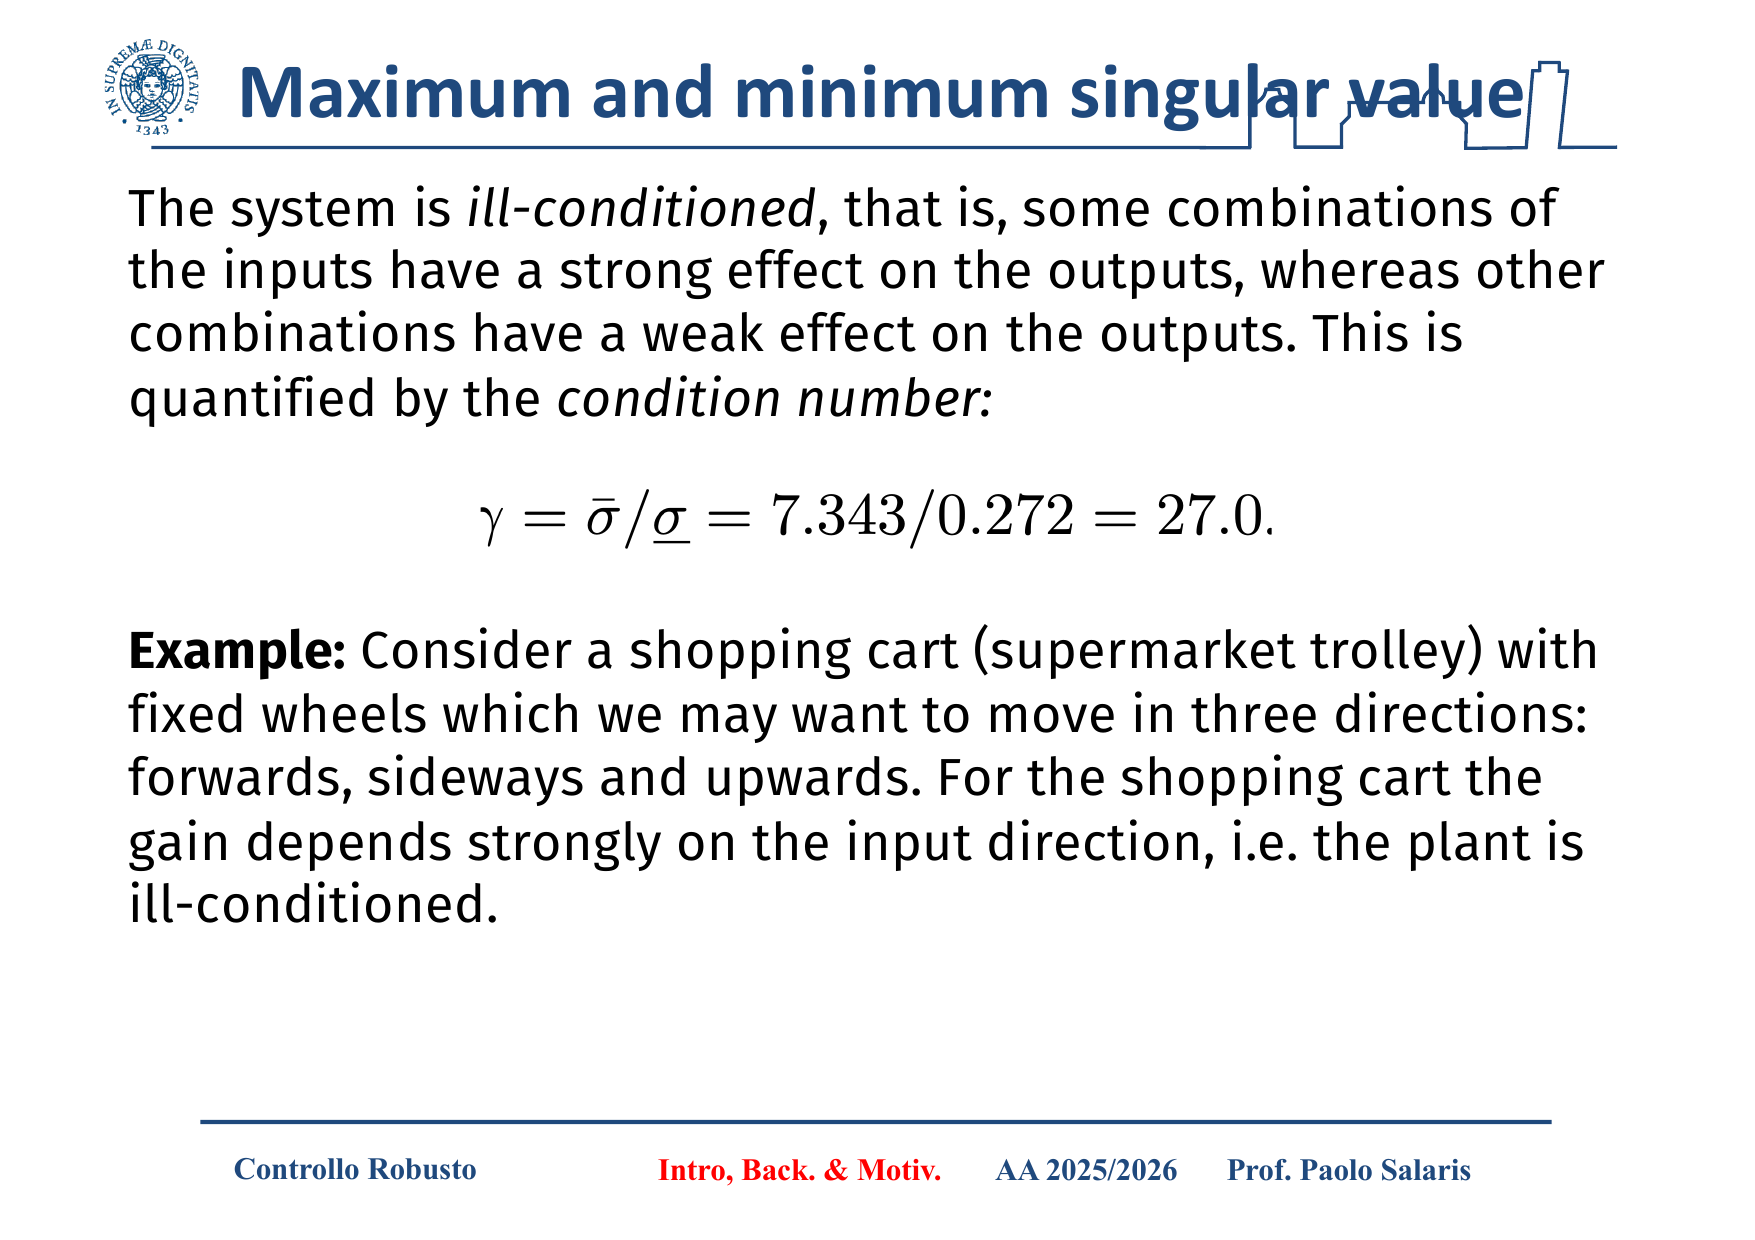
\includegraphics[width=\linewidth]{images3/slide-28.png}
        \caption{Il numero di condizionamento misura quanto il sistema sia anisotropo dal punto di vista del guadagno.}
    \end{subfigure}
    \caption{La parte finale della lezione traduce la SVD in una misura concreta della difficoltà di controllo del processo.}
\end{figure}

\begin{figure}[H]
    \centering
    \begin{subfigure}{0.48\textwidth}
        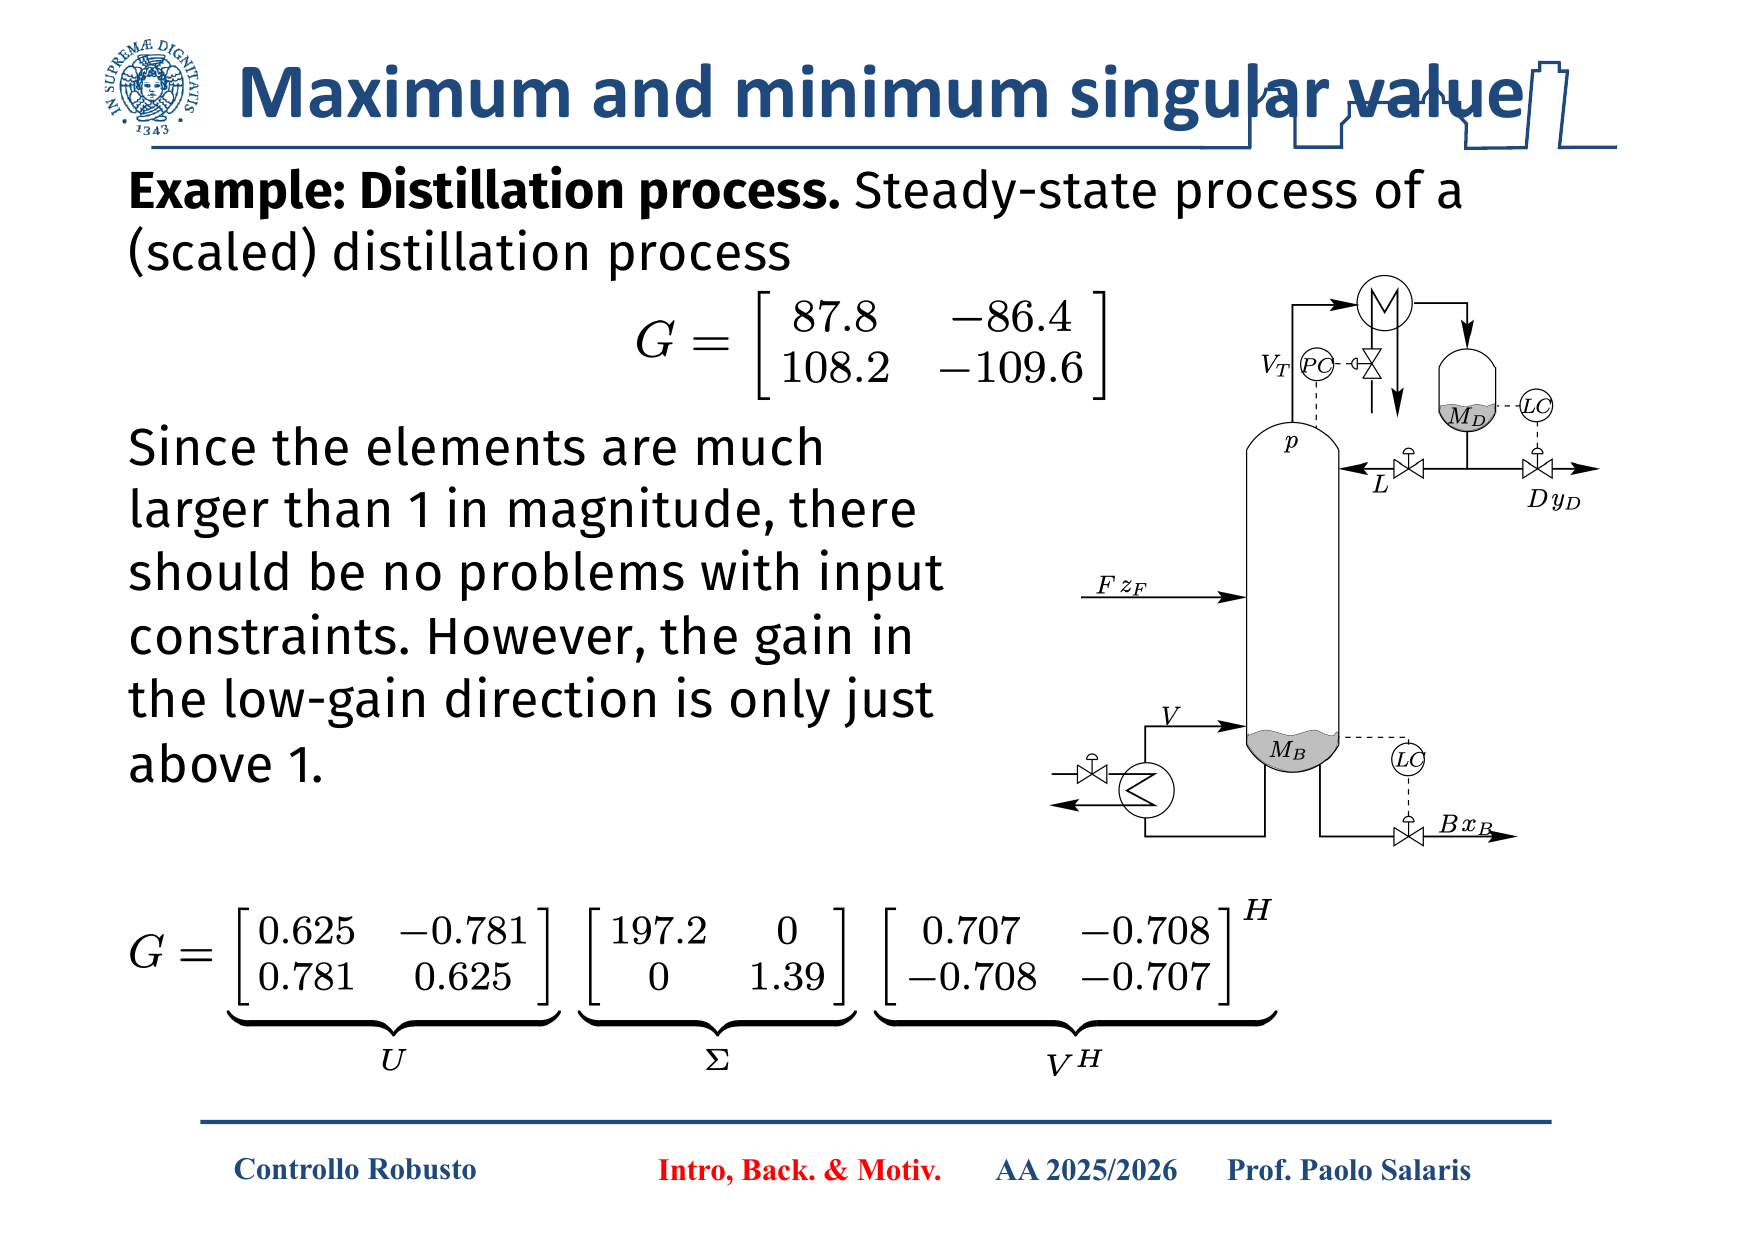
\includegraphics[width=\linewidth]{images3/slide-29.png}
        \caption{Nel processo di distillazione i grandi coefficienti di matrice non impediscono la presenza di una direzione debole.}
    \end{subfigure}
    \hfill
    \begin{subfigure}{0.48\textwidth}
        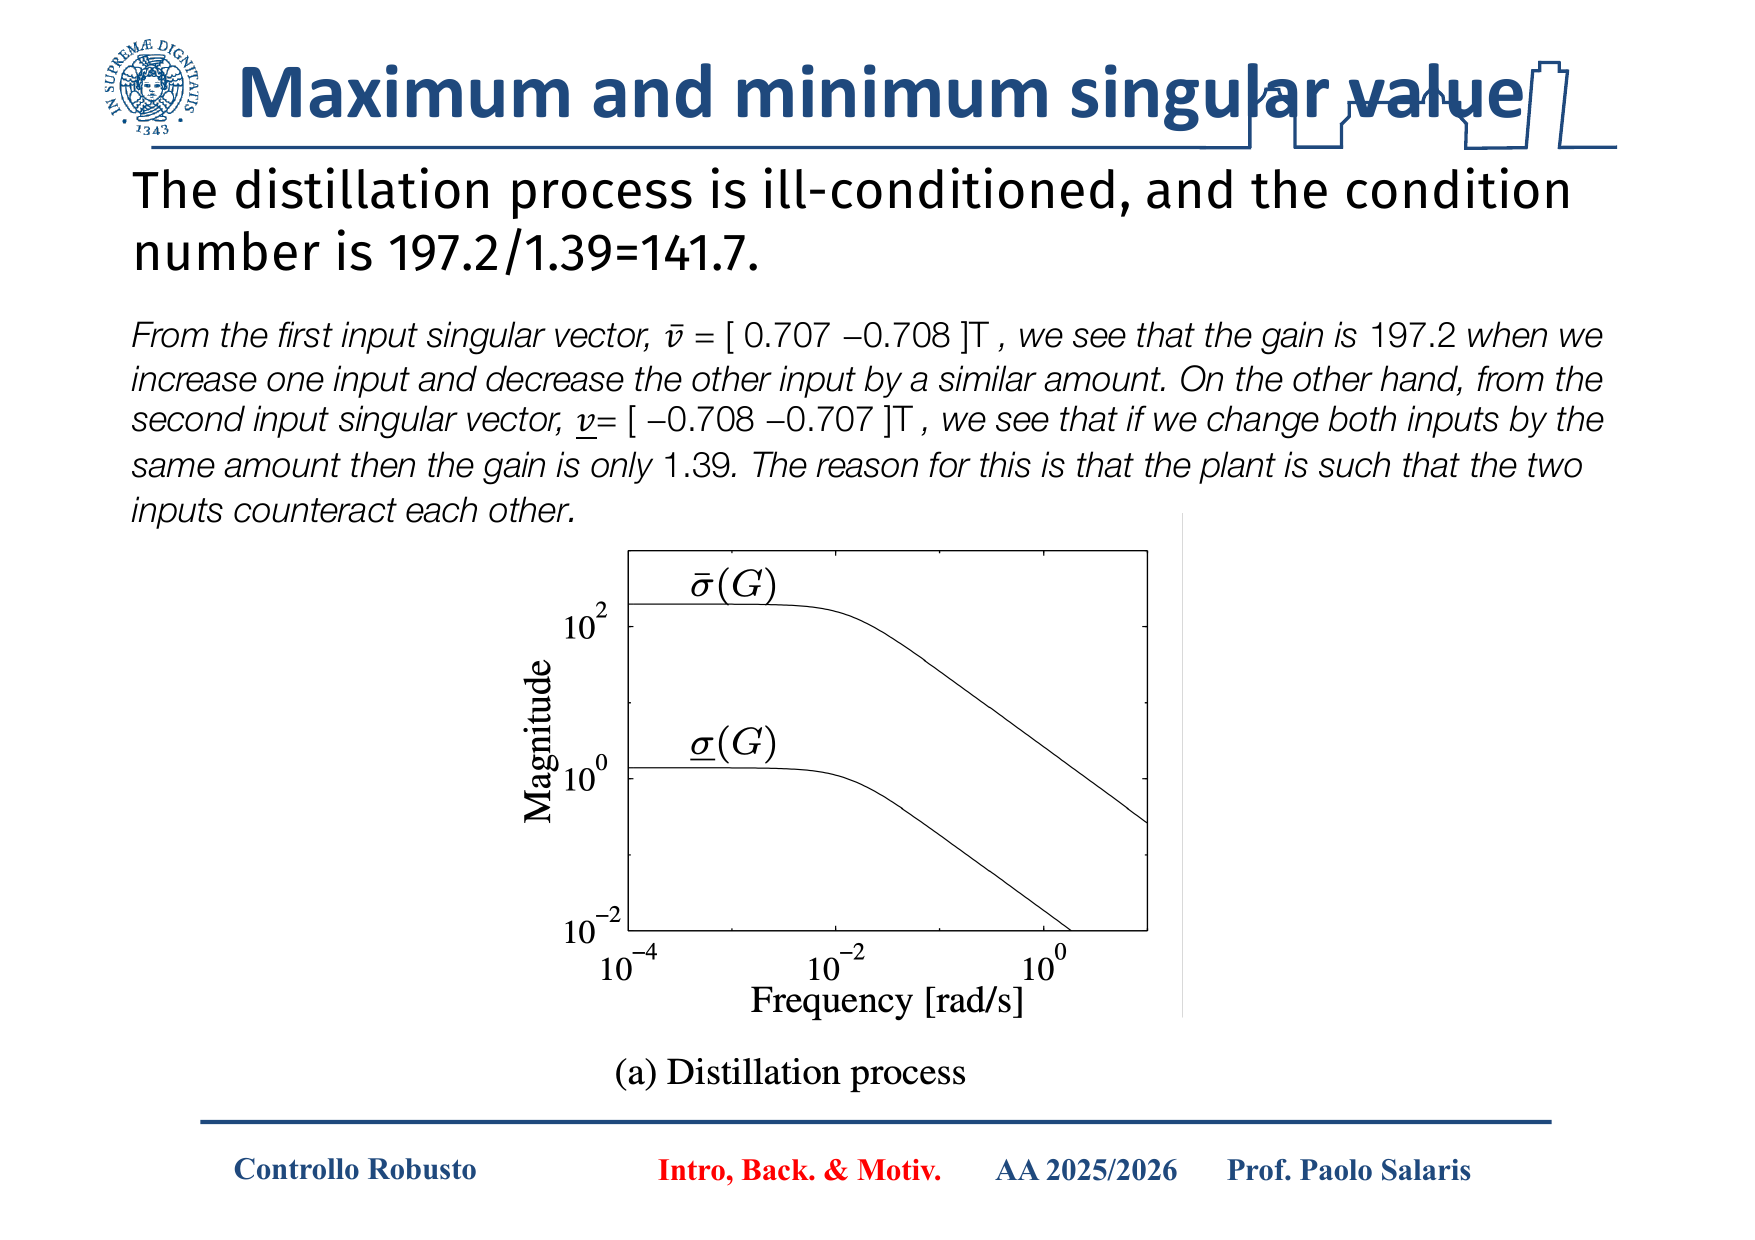
\includegraphics[width=\linewidth]{images3/slide-30.png}
        \caption{Le direzioni singolari chiariscono quali combinazioni di ingressi si rinforzano e quali invece si contrastano.}
    \end{subfigure}
    \caption{L’esempio conclusivo mostra perché il controllo robusto debba ragionare in termini di direzioni e non di soli elementi di matrice.}
\end{figure}

\subsection{Sintesi conclusiva della lezione}

Se la si legge insieme alla Lezione 3 e alla Lezione 5, questa lezione appare come il vero punto di cerniera del capitolo. La Lezione 3 aveva introdotto stabilità interna, specifiche statiche e dinamiche, e la comparsa iniziale della funzione di sensitività come filtro dell’incertezza di modello. La Lezione 4 prende queste idee e le organizza in un quadro unitario: return difference, funzioni $S$ e $T$, banda passante, controllo a due gradi di libertà, generalizzazione matriciale e guadagni direzionali.

Nel caso SISO il messaggio fondamentale è che tracking, rigetto dei disturbi e attenuazione del rumore non sono richieste separate, ma diverse facce dello stesso problema di distribuzione della sensitività in frequenza. Nel caso MIMO la stessa logica sopravvive, ma richiede un linguaggio più ricco: matrici di sensitività, norme indotte, valori singolari, SVD e numero di condizionamento.

La Lezione 5 potrà allora partire da qui in modo naturale. Una volta chiarito che cosa significhi rendere un canale ``piccolo'' o ``grande'' nelle varie frequenze e nelle varie direzioni, il passo successivo non sarà più concettualmente difficile: si tratterà di trasformare queste idee in vere regole di progetto sul loop transfer, sui guadagni principali e sul loop shaping. In questo senso la Lezione 4 non è soltanto un capitolo intermedio, ma il ponte necessario fra l’analisi della robustezza e la sintesi del controllore.

\clearpage
\phantomsection
\section*{Appendice}
\addcontentsline{toc}{section}{Appendice}

\subsection*{Nota sulle convenzioni di segno}
\phantomsection
\addcontentsline{toc}{subsection}{Nota sulle convenzioni di segno}

Nel corso del documento possono comparire convenzioni diverse per il segno della retroazione e quindi per la scrittura di quantità come $1+L(s)$ oppure $1-L(s)$. Non c’è contraddizione concettuale: ciò che conta è mantenere coerenza interna fra definizione del loop transfer, punto critico del criterio di Nyquist e definizione di sensibilità e sensibilità complementare.

\subsection*{Riferimento al materiale originale}
\phantomsection
\addcontentsline{toc}{subsection}{Riferimento al materiale originale}

Questo elaborato è una traduzione e rielaborazione estesa del materiale didattico del corso di Controllo Robusto A.A. 2025/2026 caricato dall’utente come base di lavoro.

\begin{coverpage}
\centering
{\Huge\bfseries Controllo Robusto\par}
\vspace{0.4em}
{\LARGE Traduzione in italiano e approfondimento\par}
\vspace{0.5em}
{\Large Guadagni principali, loop shaping e margini di stabilità\par}
\vfill

\includegraphics[width=0.78\textwidth]{images4/slide-01.png}
\vfill
\begin{focusbox}
\textbf{Obiettivo del documento.} Questa parte del testo riorganizza e approfondisce il blocco di slide dedicato ai \emph{principal gains}, al \emph{loop shaping} SISO e MIMO, al confronto tra controllo a uno e due gradi di libertà e al legame fra margini di stabilità e prestazioni in norma infinita. Le immagini originali delle slide sono state inserite nel testo per mantenere il collegamento diretto con il materiale del corso.
\end{focusbox}
\vfill
{\large Basato sulle slide del corso AA 2025/2026\par}
\end{coverpage}

\section{Lezione 5}

\subsection{Visione d'insieme della lezione}

Questa lezione porta a maturazione il punto di vista introdotto nella Lezione 4. Lì erano state definite le matrici di sensibilità e di sensibilità complementare; qui tali grandezze vengono usate per ricavare vere e proprie regole di progetto. L'idea guida è che le prestazioni del sistema chiuso possano essere lette osservando i \emph{guadagni principali}, cioè i valori singolari delle matrici di trasferimento rilevanti, e che il problema di progetto possa essere riformulato come un problema di \emph{shape} del loop transfer nelle varie bande di frequenza.

Il materiale segue una progressione molto istruttiva. Prima chiarisce quali canali dell'anello chiuso devono essere piccoli per garantire buon tracking e buon rigetto dei disturbi. Poi mostra perché questo richieda alti guadagni d'anello alle basse frequenze, ma anche perché tali guadagni non possano essere spinti arbitrariamente in alto: incertezza di modello, rumore di misura e saturazione degli attuatori impongono limiti precisi. Su questa base nasce il \emph{loop shaping}: invece di progettare direttamente il chiuso, si modella la funzione d'anello aperto in modo che soddisfi simultaneamente vincoli di prestazione e di robustezza.

Nella seconda parte della lezione il ragionamento viene tradotto in pratica. Si discute la procedura standard di loop shaping nel caso SISO e la sua estensione al caso MIMO, evidenziandone però le limitazioni. Successivamente si confrontano architetture a uno e due gradi di libertà e si spiega perché il feedback resti indispensabile anche quando, in linea di principio, il feed-forward sembrerebbe poter invertire perfettamente il processo. Infine il capitolo chiude il cerchio collegando stabilità, margini di guadagno e di fase, e specifiche di prestazione in termini delle norme di $S$ e $T$.

\begin{keybox}
La morale della lezione è molto concreta: un buon controllore robusto non è quello che massimizza il guadagno ovunque, ma quello che distribuisce il guadagno in frequenza nel modo corretto. Alle basse frequenze il loop deve essere forte per seguire il riferimento e rigettare i disturbi; alle alte frequenze deve invece indebolirsi per non amplificare rumore, incertezza e attività di controllo.
\end{keybox}

\begin{focusbox}
\textbf{Mappa mentale della lezione.} Per non perdersi nelle formule conviene tenere separati tre livelli. Il primo livello sono i canali chiusi: $S$, $T$, $S_o$, $T_o$, $S_i$, $T_i$. Il secondo livello sono i guadagni principali, cioè i valori singolari che misurano quanto quei canali amplificano ingressi in ogni direzione. Il terzo livello è il progetto: scegliere $K$ in modo che il loop $L$ renda piccoli i canali giusti nelle bande giuste, senza perdere margini di stabilità.
\end{focusbox}

\subsection{Guadagni principali e canali fondamentali del sistema chiuso}

Le prime slide riprendono la struttura MIMO standard con riferimento $r$, rumore di misura $n$, disturbo di ingresso al processo $d_i$ e disturbo di uscita $d$. Se si introducono le matrici di anello
$$
L_o = PK,
\qquad
L_i = KP,
$$
e le corrispondenti matrici di sensitività
$$
S_o = (I + PK)^{-1},
\qquad
T_o = PK(I + PK)^{-1},
$$
$$
S_i = (I + KP)^{-1},
\qquad
T_i = KP(I + KP)^{-1},
$$
allora i segnali chiusi possono essere espressi in modo molto compatto come
\begin{align*}
y &= T_o(r-n) + S_o P d_i + S_o d, \\
e &= r-y = S_o(r-d) + T_o n - S_o P d_i, \\
u &= K S_o(r-n) - K S_o d - T_i d_i, \\
u_p &= u + d_i = K S_o(r-n) - K S_o d + S_i d_i.
\end{align*}

Queste identità vanno lette lentamente, perché contengono già tutto il progetto robusto. Il riferimento e il rumore di misura attraversano $T_o$; i disturbi applicati all'uscita del processo attraversano $S_o$; i disturbi applicati prima del processo attraversano $S_oP$ sull'uscita e $S_i$ sull'ingresso del processo. In altre parole, la qualità del comportamento chiuso dipende dal fatto che certe matrici risultino piccole o grandi nelle bande giuste.

Le slide parlano di \emph{principal gains}. Nel caso MIMO questo termine coincide con i valori singolari della matrice di trasferimento. Per una matrice $M(j\omega)$, il massimo valore singolare $\bar{\sigma}(M(j\omega))$ misura il massimo guadagno che il sistema può realizzare alla frequenza $\omega$ scegliendo la direzione più sfavorevole dell'ingresso; il minimo valore singolare $\underline{\sigma}(M(j\omega))$ misura invece la direzione meno amplificata. Di conseguenza, richiedere che un certo canale sia ``piccolo'' significa imporre che il suo massimo valore singolare sia piccolo per tutte le direzioni rilevanti.

\begin{figure}[H]
    \centering
    
\includegraphics[width=0.8\textwidth]{images4/slide-01.png}
    \caption{Prima slide del capitolo: i canali fondamentali fra riferimento, disturbi, rumore, uscita e segnale di controllo sono espressi in funzione di $S_o$, $T_o$, $S_i$ e $T_i$.}
\end{figure}

\subsection{Quali canali devono essere piccoli}

Dal punto di vista delle prestazioni, le richieste naturali sono le seguenti.
\begin{itemize}
    \item Per rigettare bene il disturbo di uscita $d$ sull'uscita $y$, deve essere piccolo il canale $S_o$.
    \item Per attenuare il disturbo di ingresso $d_i$ sull'uscita $y$, deve essere piccolo il canale $S_o P$.
    \item Per limitare l'effetto di $d_i$ sull'ingresso effettivo del processo $u_p$, deve essere piccolo $S_i$.
    \item Per limitare l'effetto di $d$ sul comando $u$, deve essere piccolo $K S_o$, equivalentemente $S_i K$.
\end{itemize}

In formule, la richiesta si traduce tipicamente nel voler rendere piccole quantità del tipo
$$
\bar{\sigma}(S_o),
\qquad
\bar{\sigma}(S_o P),
\qquad
\bar{\sigma}(S_i),
\qquad
\bar{\sigma}(S_i K),
$$
nelle bande di frequenza in cui i rispettivi disturbi sono energeticamente importanti. Le slide ricordano che, in molte applicazioni, i disturbi fisici lenti e le variazioni del carico si concentrano prevalentemente alle basse frequenze. Per questo il problema del rigetto dei disturbi è, in prima approssimazione, un problema di progetto del loop gain in bassa frequenza.

Un primo legame quantitativo si ottiene osservando che
$$
S_o = (I + PK)^{-1},
\qquad
S_i = (I + KP)^{-1}.
$$
Usando le disuguaglianze sui valori singolari,
$$
\underline{\sigma}(PK)-1 \le \underline{\sigma}(I+PK) \le \bar{\sigma}(I+PK) \le \bar{\sigma}(PK)+1,
$$
e analogamente
$$
\underline{\sigma}(KP)-1 \le \underline{\sigma}(I+KP) \le \bar{\sigma}(I+KP) \le \bar{\sigma}(KP)+1,
$$
si deduce che, se il minimo valore singolare del loop gain è ben maggiore di $1$, allora i canali di sensitività diventano piccoli. Il passaggio importante è questo:
$$
\bar{\sigma}(S_o)
= \frac{1}{\underline{\sigma}(I+PK)}
\le \frac{1}{\underline{\sigma}(PK)-1}
\qquad
\text{se } \underline{\sigma}(PK)>1,
$$
e analogamente
$$
\bar{\sigma}(S_i)
= \frac{1}{\underline{\sigma}(I+KP)}
\le \frac{1}{\underline{\sigma}(KP)-1}
\qquad
\text{se } \underline{\sigma}(KP)>1.
$$
La slide usa correttamente il simbolo $\gg 1$: non basta leggere questa formula come una soglia secca. Se $\underline{\sigma}(PK)$ è appena maggiore di $1$, il bound può essere ancora grande; se invece $\underline{\sigma}(PK)\gg 1$, allora $\bar{\sigma}(S_o)\ll 1$. Lo stesso ragionamento vale per $S_i$ e $KP$.

Questa è la prima conclusione forte delle slide: \emph{buon rigetto dei disturbi equivale, in modo molto diretto, a grande guadagno d'anello alle basse frequenze}. Nel caso MIMO non basta però guardare un solo modulo: bisogna assicurarsi che il loop gain sia grande in tutte le direzioni rilevanti, cioè che sia grande anche il suo minimo valore singolare.

\begin{figure}[H]
    \centering
    \begin{subfigure}{0.48\textwidth}
        
\includegraphics[width=\linewidth]{images4/slide-02.png}
        \caption{Legame tra grandezza del loop gain e picco delle matrici di sensitività.}
    \end{subfigure}
    \hfill
    \begin{subfigure}{0.48\textwidth}
        
\includegraphics[width=\linewidth]{images4/slide-03.png}
        \caption{Interpretazione delle condizioni di prestazione sui diversi canali dell'anello chiuso.}
    \end{subfigure}
    \caption{Per ottenere buon rigetto dei disturbi bisogna rendere piccolo il massimo guadagno delle matrici $S_o$, $S_oP$, $S_i$ e $S_iK$ nelle bande rilevanti.}
\end{figure}

Le slide fanno anche un passo ulteriore assumendo $P$ e $K$ invertibili. In questo caso
$$
S_o P = (P^{-1}+K)^{-1},
\qquad
K S_o = (P + K^{-1})^{-1}.
$$
Queste identità si ottengono semplicemente raccogliendo $P$ oppure $K$:
$$
(I+PK)^{-1}P
= \bigl(P^{-1}(I+PK)\bigr)^{-1}
= (P^{-1}+K)^{-1},
$$
e
$$
K(I+PK)^{-1}
= \bigl((I+PK)K^{-1}\bigr)^{-1}
= (K^{-1}+P)^{-1}.
$$
Servono a capire due canali che spesso creano confusione. Se il loop è molto grande, allora $P^{-1}$ diventa piccolo rispetto a $K$ e $K^{-1}$ diventa piccolo rispetto a $P$; quindi, in prima approssimazione,
$$
S_oP \simeq K^{-1},
\qquad
KS_o \simeq P^{-1}.
$$
In termini di valori singolari, la slide riassume questa idea come
$$
\bar{\sigma}(S_oP) \simeq \bar{\sigma}(K^{-1})
= \frac{1}{\underline{\sigma}(K)},
\qquad
\bar{\sigma}(KS_o) \simeq \bar{\sigma}(P^{-1})
= \frac{1}{\underline{\sigma}(P)}.
$$
Quindi la sola grandezza del loop transfer non basta sempre: il rigetto del disturbo di ingresso visto in uscita dipende anche dal fatto che il controllore abbia guadagno sufficiente, mentre il rigetto del disturbo di uscita visto sul comando dipende anche dal fatto che il processo non abbia guadagno troppo piccolo nella banda considerata.

Per questo la slide riassume le richieste così:
\begin{itemize}
    \item buona prestazione sull'uscita $y$ richiede $\underline{\sigma}(L_o)=\underline{\sigma}(PK)\gg 1$ nelle frequenze in cui è significativo $d$, e $\underline{\sigma}(K)\gg 1$ nelle frequenze in cui è significativo $d_i$;
    \item buona prestazione all'ingresso del processo $u_p$ richiede $\underline{\sigma}(L_i)=\underline{\sigma}(KP)\gg 1$ nelle frequenze in cui è significativo $d_i$, e $\underline{\sigma}(P)\gg 1$ nelle frequenze in cui è significativo $d$.
\end{itemize}

\begin{figure}[H]
    \centering
    \begin{subfigure}{0.48\textwidth}
        
\includegraphics[width=\linewidth]{images4/slide-04.png}
        \caption{Il messaggio operativo della progettazione MIMO: servono alti loop gains nelle bande necessarie.}
    \end{subfigure}
    \hfill
    \begin{subfigure}{0.48\textwidth}
        
\includegraphics[width=\linewidth]{images4/slide-05.png}
        \caption{Introduzione del primo grande trade-off: prestazione contro robustezza rispetto all'incertezza di modello.}
    \end{subfigure}
    \caption{Il loop gain deve essere grande dove serve la prestazione, ma non può essere grande ovunque senza conseguenze sulla robustezza.}
\end{figure}

\subsection{Perché il guadagno non può essere grande ovunque}

\subsubsection{Incertezza di modello}

La prima limitazione discussa nelle slide riguarda la robustezza rispetto agli errori di modello. Si considera un processo perturbato del tipo
$$
P_\Delta = (I+\Delta)P,
$$
dove $\Delta$ è stabile e il sistema nominale è internamente stabile. La slide lavora sul determinante della matrice caratteristica del sistema perturbato:
$$
\det\!\bigl(I+(I+\Delta)PK\bigr).
$$
Ponendo $L_o=PK$ e $T_o=L_o(I+L_o)^{-1}$, si ottiene la fattorizzazione a livello di determinante
$$
\det\!\bigl(I+(I+\Delta)PK\bigr)
=
\det(I+PK)\,\det(I+\Delta T_o).
$$
Nel caso MIMO conviene scriverla così, e non come una semplice uguaglianza fra matrici, perché i fattori non commutano in generale. Ne segue che, una volta fissata la stabilità nominale, la stabilità del sistema perturbato dipende dal fatto che
$$
\det(I+\Delta T_o)
$$
non abbia zeri nel semipiano destro.

Questa relazione è fondamentale perché porta a una classica condizione di piccolo guadagno:
$$
\|\Delta T_o\|_\infty < 1
$$
oppure, frequenza per frequenza,
$$
\bar{\sigma}(\Delta(j\omega)T_o(j\omega)) < 1.
$$
Se l'incertezza di modello è significativa soprattutto alle alte frequenze, allora bisogna imporre che $T_o$ sia piccolo proprio in alta frequenza. Ma $T_o = L_o(I+L_o)^{-1}$ è piccolo alle alte frequenze quando il loop gain decresce. Ecco perché il medesimo progetto che richiede alto loop gain in bassa frequenza per il rigetto dei disturbi richiede invece basso loop gain in alta frequenza per la robustezza.

\subsubsection{Rumore di misura}

La seconda limitazione è il rumore di misura $n$. Dalla relazione
$$
y = T_o(r-n) + S_o P d_i + S_o d
$$
si vede che il rumore entra sull'uscita attraverso $T_o$. Se si rende il loop gain molto grande anche alle alte frequenze, allora $T_o \approx I$ in una banda troppo ampia e il rumore di misura viene trasmesso quasi integralmente all'uscita. In pratica il feedback, anziché proteggere il sistema, comincia a inseguire il rumore del sensore.

Questo è un punto tipico dei sistemi reali. I disturbi fisici sul processo sono spesso lenti, mentre il rumore di misura è prevalentemente veloce. La stessa scelta di progetto che è ottima per i primi può quindi essere pessima per il secondo. Ancora una volta, il progetto robusto consiste nel distribuire il guadagno in frequenza nel modo corretto, non nel massimizzarlo senza criterio.

\subsubsection{Attività di controllo e saturazione}

Le slide richiamano poi un'altra conseguenza pratica: un loop gain troppo alto fuori dalla banda utile del processo può generare comandi inaccettabili. Se, per esempio, $P(j\omega)$ è quadrata e invertibile, $\bar{\sigma}(P(j\omega)) \ll 1$ ad alta frequenza, ma si impone comunque un loop gain grande, allora l'inverso $P^{-1}(j\omega)$ può avere guadagno enorme. Infatti
$$
\bar{\sigma}\!\left(P^{-1}(j\omega)\right)
= \frac{1}{\underline{\sigma}(P(j\omega))},
$$
perciò quando $\underline{\sigma}(P(j\omega))$ è piccolo il controllore è costretto a generare comandi molto grandi per ottenere un effetto apprezzabile sull'uscita.

Il passaggio algebrico mostrato nella slide è il seguente. Partendo da
$$
u = KS_o(r-n-d) - T_i d_i
= S_iK(r-n-d)-T_i d_i,
$$
se il loop è molto grande nella banda considerata si ha $S_iK\simeq P^{-1}$ e $T_i\simeq I$. Quindi
$$
u \simeq P^{-1}(r-n-d)-d_i.
$$
Questa formula è molto utile perché spiega il fenomeno fisico: in alta frequenza, dove il processo attenua molto, chiedere prestazioni aggressive equivale a chiedere al controllore di invertire una dinamica sfavorevole. Il risultato può essere saturazione degli attuatori, amplificazione del rumore e perdita di robustezza.

Anche quando il loop gain è piccolo, mantenere un guadagno del controllore troppo elevato può essere pericoloso. Se infatti $L_o$ o $L_i$ sono molto minori di $1$ in un certo intervallo di frequenze, allora $S_o\simeq I$ e $T_i\simeq 0$, per cui
$$
u=KS_o(r-n-d)-T_i d_i \simeq K(r-n-d).
$$
In questa situazione il processo non chiude efficacemente l'anello, ma il controllore continua ad amplificare direttamente riferimento, rumore e disturbo. Per questo le slide non chiedono soltanto loop gain basso in alta frequenza: chiedono anche che $\bar{\sigma}(K)$ non diventi inutilmente grande.

\begin{figure}[H]
    \centering
    \begin{subfigure}{0.48\textwidth}
        
\includegraphics[width=\linewidth]{images4/slide-06.png}
        \caption{Rumore di misura e attività di controllo limitano il guadagno ammissibile alle alte frequenze.}
    \end{subfigure}
    \hfill
    \begin{subfigure}{0.48\textwidth}
        
\includegraphics[width=\linewidth]{images4/slide-07.png}
        \caption{Riassunto delle richieste sulle bande di bassa e alta frequenza.}
    \end{subfigure}
    \caption{Le prestazioni in uscita, la robustezza e l'ammissibilità del comando impongono richieste opposte in bassa e alta frequenza.}
\end{figure}

Il grafico riassuntivo delle slide rappresenta esattamente questo compromesso. In bassa frequenza si vogliono valori grandi del loop gain, così da avere sensitività piccola e buon rigetto dei disturbi. In alta frequenza si vogliono invece valori piccoli del loop gain, così da avere buona robustezza e bassa trasmissione del rumore. Fra le due regioni esiste necessariamente una zona di transizione, la regione di crossover, che diventa il punto più delicato del progetto.

\begin{figure}[H]
    \centering
    
\includegraphics[width=0.72\textwidth]{images4/slide-08.png}
    \caption{Schema qualitativo di loop shaping: guadagni grandi alle basse frequenze, guadagni piccoli alle alte frequenze e regione di crossover da modellare con attenzione.}
\end{figure}

\begin{focusbox}
\textbf{Regola pratica del capitolo.} Alle basse frequenze, tipicamente $\omega\in(0,\omega_B)$, si cerca
$$
\underline{\sigma}(PK)\gg 1,
\qquad
\underline{\sigma}(KP)\gg 1,
\qquad
\underline{\sigma}(K)\gg 1,
$$
per ottenere buon rigetto dei disturbi e buon tracking. Alle alte frequenze, tipicamente $\omega\in(\omega_B,\infty)$, si cerca invece
$$
\bar{\sigma}(PK)\ll 1,
\qquad
\bar{\sigma}(KP)\ll 1,
\qquad
\bar{\sigma}(K)<K_M,
$$
dove $K_M$ è un limite pratico non troppo grande, imposto da rumore di misura e saturazione degli attuatori.
\end{focusbox}

\subsection{Loop shaping nel caso SISO}

Nel caso SISO i valori singolari si riducono al modulo della funzione di trasferimento e il problema diventa più intuitivo. Le slide descrivono una procedura molto classica:
\begin{enumerate}
    \item si sceglie una funzione d'anello desiderata $L(s)$, razionale e strettamente propria, che incorpori i poli e gli zeri nel semipiano destro del processo $P(s)$;
    \item si impone che $|L(j\omega)|$ superi i vincoli di prestazione alle basse frequenze e resti sotto i vincoli di robustezza alle alte frequenze;
    \item si richiede che $1+L(s)$ abbia tutti gli zeri nel semipiano sinistro aperto, così che il comportamento nella zona di crossover resti ben controllato;
    \item una volta costruita $L$, si pone
    $$
    K(s)=\frac{L(s)}{P(s)}.
    $$
\end{enumerate}

Questa procedura rende molto chiaro il significato del loop shaping: non si parte dal controllore per vedere ``che cosa succede'', ma si decide prima quale forma dovrà avere l'anello aperto per soddisfare contemporaneamente prestazione e robustezza, e solo alla fine si ricava il controllore.

\begin{figure}[H]
    \centering
    
\includegraphics[width=0.8\textwidth]{images4/slide-09.png}
    \caption{Procedura di loop shaping nel caso SISO: si sceglie direttamente la forma desiderata di $L(s)$ e poi si ricava il controllore come $K=L/P$.}
\end{figure}

\subsection{Loop shaping nel caso MIMO e sue limitazioni}

Nel caso MIMO l'idea di base resta la stessa, ma la realizzazione pratica diventa più difficile. Prima si sceglie quale loop si vuole modellare:
$$
L_o=PK
\qquad \text{oppure} \qquad
L_i=KP.
$$
Poi si cerca una matrice d'anello $L(s)$ strettamente propria tale che:
\begin{itemize}
    \item contenga i poli e gli zeri nel semipiano destro del processo;
    \item non introduca cancellazioni instabili in $P^{-1}L$ oppure in $LP^{-1}$;
    \item abbia $\underline{\sigma}(L(j\omega))$ sufficientemente grande alle basse frequenze per la prestazione;
    \item abbia $\bar{\sigma}(L(j\omega))$ sufficientemente piccolo alle alte frequenze per la robustezza;
    \item soddisfi la condizione di stabilità
    $$
    \det(I+L(s)) \neq 0
    $$
    nel semipiano destro, cioè abbia tutti gli zeri di $\det(I+L)$ nel semipiano sinistro aperto.
\end{itemize}

In tal caso il controllore si ricava in modo diverso a seconda del loop scelto:
$$
K=P^{-1}L_o
\qquad
\text{se } L=L_o=PK,
$$
oppure
$$
K=L_iP^{-1}
\qquad
\text{se } L=L_i=KP.
$$
Questa distinzione è piccola nella scrittura ma grande nel significato: nel MIMO l'ordine dei fattori conta, quindi output loop e input loop non sono intercambiabili come nel caso SISO.

\begin{figure}[H]
    \centering
    \begin{subfigure}{0.48\textwidth}
        
\includegraphics[width=\linewidth]{images4/slide-10.png}
        \caption{Estensione del loop shaping al caso MIMO.}
    \end{subfigure}
    \hfill
    \begin{subfigure}{0.48\textwidth}
        
\includegraphics[width=\linewidth]{images4/slide-11.png}
        \caption{Primo limite: la traduzione di specifiche direzionali in limiti uniformi sul loop gain introduce conservativismo.}
    \end{subfigure}
    \caption{Nel caso MIMO il progetto resta concettualmente analogo al caso SISO, ma le disuguaglianze scalari non catturano più tutta la struttura del problema.}
\end{figure}

Il punto davvero importante della lezione è però che questa procedura, pur elegante, può essere troppo conservativa. Nelle slide questo fatto viene espresso introducendo due pesi matriciali: $W_t$, che descrive la taglia e la dipendenza in frequenza dell'incertezza di modello, e $W_s$, che descrive l'inviluppo desiderato per la sensitività nominale. Per esempio, se si rappresenta un'incertezza moltiplicativa come
$$
P_\Delta = (I+\Delta)P,
\qquad
\Delta=\tilde{\Delta}W_t,
\qquad
\bar{\sigma}(\tilde{\Delta}) < 1.
$$
allora, per il teorema del piccolo guadagno, una condizione naturale di robustezza è
$$
\bar{\sigma}(W_t T_o) < 1.
$$
Questa è la condizione da ricordare: il peso $W_t$ non va confrontato da solo con il loop, ma con il canale chiuso $T_o$. Se però si vuole imporre questa richiesta tramite un semplice vincolo uniforme sul loop gain, si è costretti a sovrastimare:
$$
\bar{\sigma}(W_t T_o)
\le
\bar{\sigma}(W_t)\,\bar{\sigma}(T_o)
\le
\bar{\sigma}(W_t)\,\frac{\bar{\sigma}(L_o)}{1-\bar{\sigma}(L_o)},
\qquad
\bar{\sigma}(L_o)<1.
$$
Da qui segue una condizione sufficiente del tipo
$$
\bar{\sigma}(L_o) < \frac{1}{\bar{\sigma}(W_t)+1}.
$$
Il problema è che tale stima ignora completamente la struttura direzionale di $W_t$ e di $T_o$: trasforma un requisito matriciale in un semplice bound scalare uniforme. In altre parole, impone che tutte le direzioni del loop siano piccole, anche se magari l'incertezza pesa davvero solo alcune direzioni.

Lo stesso accade per le specifiche di prestazione nominale. Se si richiede
$$
\bar{\sigma}(W_s S_o)<1,
$$
si può sovrastimare
$$
\bar{\sigma}(W_s S_o)
\le
\bar{\sigma}(W_s)\,\bar{\sigma}(S_o)
\le
\frac{\bar{\sigma}(W_s)}{\underline{\sigma}(L_o)-1},
\qquad
\underline{\sigma}(L_o)>1.
$$
Questo porta a una condizione sufficiente del tipo
$$
\underline{\sigma}(L_o) > \bar{\sigma}(W_s)+1.
$$
Ma ancora una volta si perde la struttura del problema: direzioni diverse possono avere pesi diversi, e un unico bound uniforme sulla matrice d'anello può risultare molto più restrittivo del necessario.

Le slide mostrano esplicitamente perché questo conservativismo può ingannare. Nell'esempio si considera
$$
P(s)=\frac{1}{s+1}
\begin{bmatrix}
1 & \alpha\\
0 & 1
\end{bmatrix},
$$
con pesi
$$
W_t(s)=
\begin{bmatrix}
\dfrac{s+2}{s+10} & \dfrac{\alpha(s+1)}{s+10}\\[0.8em]
0 & \dfrac{s+2}{s+10}
\end{bmatrix},
\qquad
W_s(s)=
\begin{bmatrix}
\dfrac{1}{s+1} & \dfrac{\alpha}{(s+1)(s+2)}\\[0.8em]
0 & \dfrac{1}{s+1}
\end{bmatrix}.
$$
Per $\alpha$ grande, i bound scalari ricavati da $\bar{\sigma}(W_t)$ e $\bar{\sigma}(W_s)$ sembrano sovrapporsi e quindi sembrano dire: ``non esiste spazio per progettare''. Tuttavia, scegliendo il controllore semplicissimo
$$
K=I_2,
$$
si ottiene
$$
W_sS =
\begin{bmatrix}
\dfrac{1}{s+2} & 0\\[0.8em]
0 & \dfrac{1}{s+2}
\end{bmatrix},
\qquad
W_tT =
\begin{bmatrix}
\dfrac{1}{s+10} & 0\\[0.8em]
0 & \dfrac{1}{s+10}
\end{bmatrix}.
$$
Queste due matrici sono piccole nei canali pesati corretti. Quindi l'apparente conflitto nasceva dal bound scalare, non dal problema reale.

\begin{figure}[H]
    \centering
    \begin{subfigure}{0.48\textwidth}
        
\includegraphics[width=\linewidth]{images4/slide-12.png}
        \caption{Secondo limite: le condizioni sufficienti di prestazione e robustezza possono sembrare contraddirsi.}
    \end{subfigure}
    \hfill
    \begin{subfigure}{0.48\textwidth}
        
\includegraphics[width=\linewidth]{images4/slide-13.png}
        \caption{Esempio in cui i bound si sovrappongono, ma un controllore semplice soddisfa comunque il problema.}
    \end{subfigure}
    \caption{La lezione mostra che, nel caso MIMO, l'uso di limiti scalari sul loop gain può portare a conclusioni troppo pessimistiche.}
\end{figure}

Le slide insistono su due conseguenze. La prima è che \emph{bound apparentemente contraddittori non implicano necessariamente che il problema sia impossibile}: ciò è vero solo nel caso SISO, mentre nel MIMO le direzioni contano e un controllore può sfruttare la struttura della matrice. La seconda è che, anche quando i bound non si contraddicono, trovare una matrice $L_o$ tale che
$$
K=P^{-1}L_o
$$
sia effettivamente stabilizzante può essere molto difficile, specialmente se il processo è non minimum phase o instabile.

\subsubsection{Che cosa significano davvero \texorpdfstring{$W_s$ e $W_t$}{Ws e Wt}}

Le tre slide successive, assenti nella versione iniziale degli appunti, sono preziose perché chiariscono il senso esatto dei pesi e correggono una possibile ambiguità concettuale. Nel caso scalare, se si sceglie un peso
$$
W_s(j\omega)=w(j\omega)\in\mathbb{C},
\qquad
S(j\omega)\in\mathbb{C},
$$
e si pone
$$
w^{-1}(j\omega)=S_d(j\omega),
$$
dove $S_d$ è la sensitività desiderata capace di soddisfare le specifiche di prestazione, allora richiedere
$$
|S(j\omega)| \le |S_d(j\omega)|
$$
equivale a imporre
$$
|W_s(j\omega)S(j\omega)| \le 1.
$$
Nel caso scalare, quindi, confrontare $S$ con l'inverso del peso oppure imporre il prodotto pesato sono due modi equivalenti di dire la stessa cosa:
$$
|S|<|w^{-1}|
\quad\Longleftrightarrow\quad
|w|\,|S|<1
\quad\Longleftrightarrow\quad
|W_sS|<1.
$$

Nel caso MIMO, però, questa equivalenza non può essere trasportata banalmente sui singoli massimi valori singolari. Infatti
$$
\bar{\sigma}(W_s^{-1})=\frac{1}{\underline{\sigma}(W_s)}
\neq
\frac{1}{\bar{\sigma}(W_s)}
$$
in generale, cioè appena il peso non è isotropo. La quantità
$$
\kappa(W_s)=\bar{\sigma}(W_s)\,\bar{\sigma}(W_s^{-1})
=\frac{\bar{\sigma}(W_s)}{\underline{\sigma}(W_s)}
$$
misura proprio quanto il peso è direzionalmente sbilanciato. Se $\kappa(W_s)=1$, il peso si comporta come uno scalare moltiplicato per una matrice unitaria; se $\kappa(W_s)>1$, direzioni diverse vengono pesate in modo diverso. Per questo motivo la specifica corretta resta
$$
\bar{\sigma}(W_s S_o)<1,
$$
da imporre direttamente sul prodotto pesato.

\begin{figure}[H]
    \centering
    \begin{subfigure}{0.48\textwidth}
        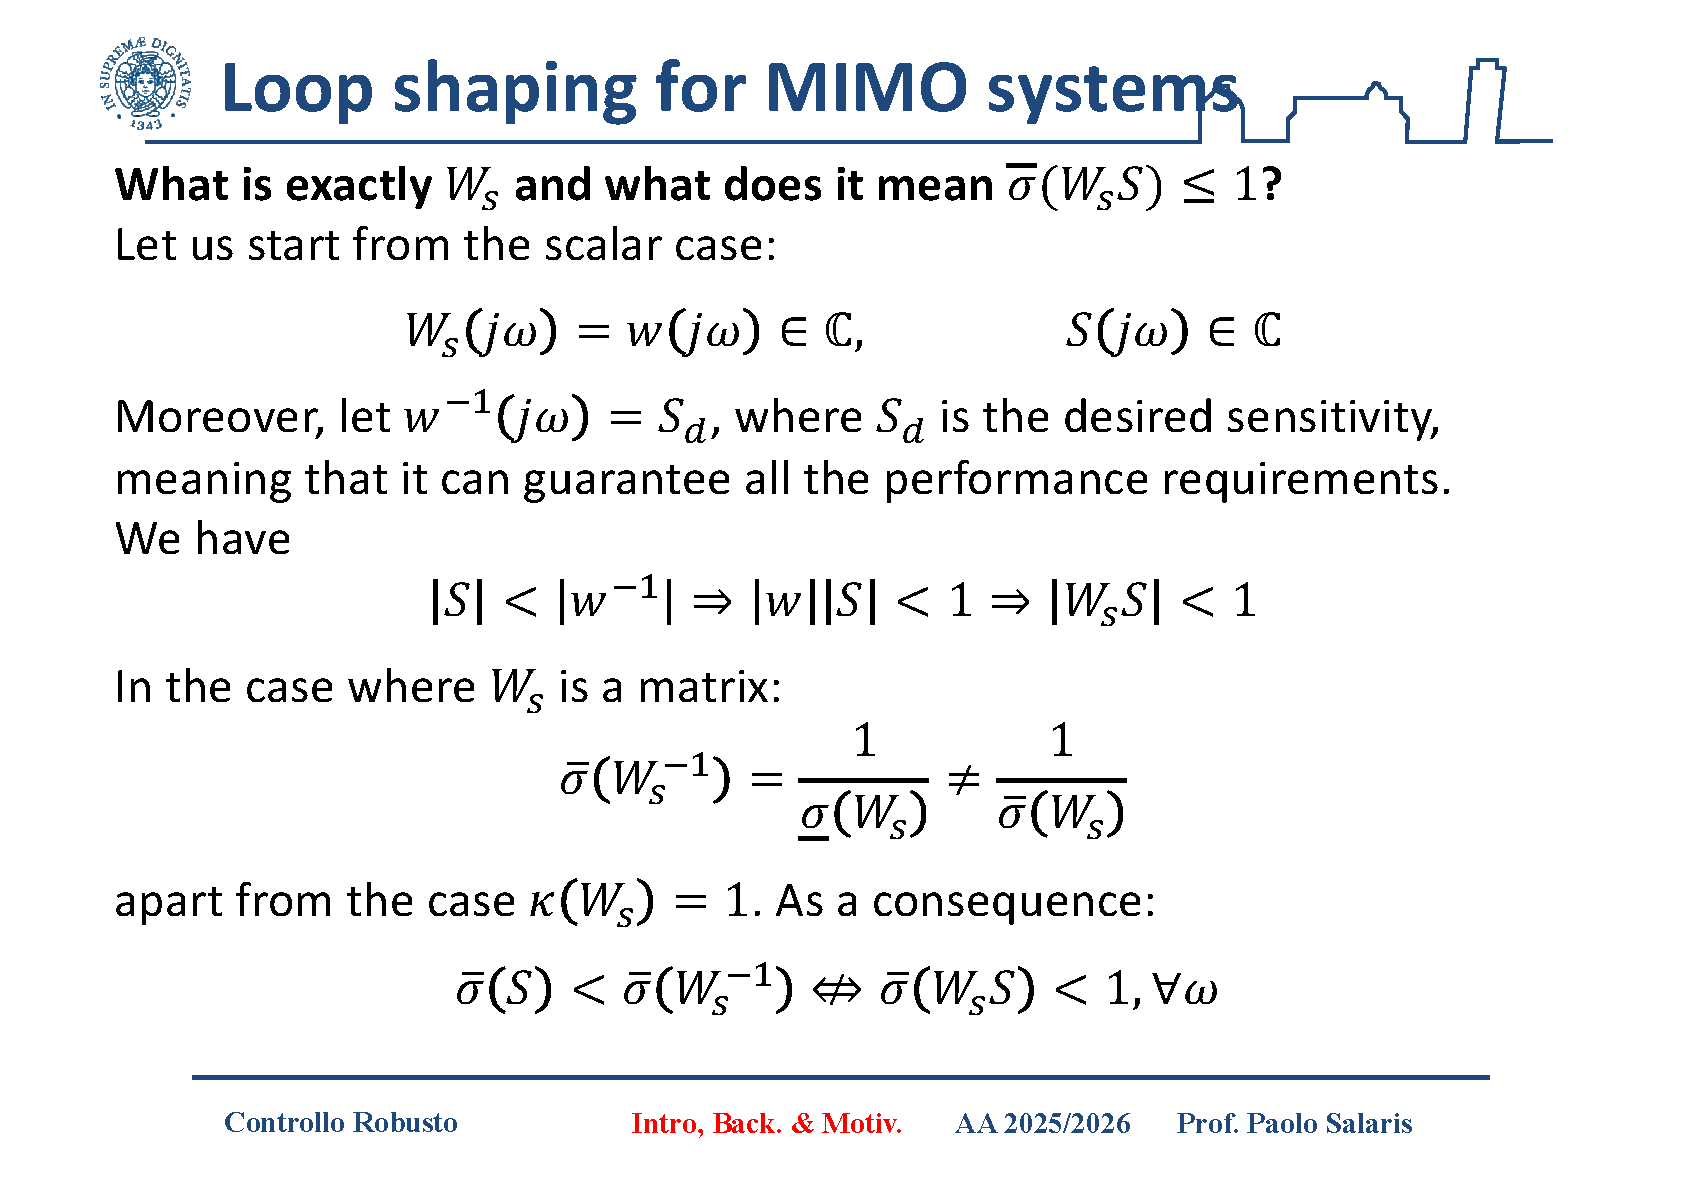
\includegraphics[width=\linewidth]{images4/slide-mimo-weights-001.png}
        \caption{Interpretazione di $W_s$ come inviluppo desiderato della sensitività.}
    \end{subfigure}
    \hfill
    \begin{subfigure}{0.48\textwidth}
        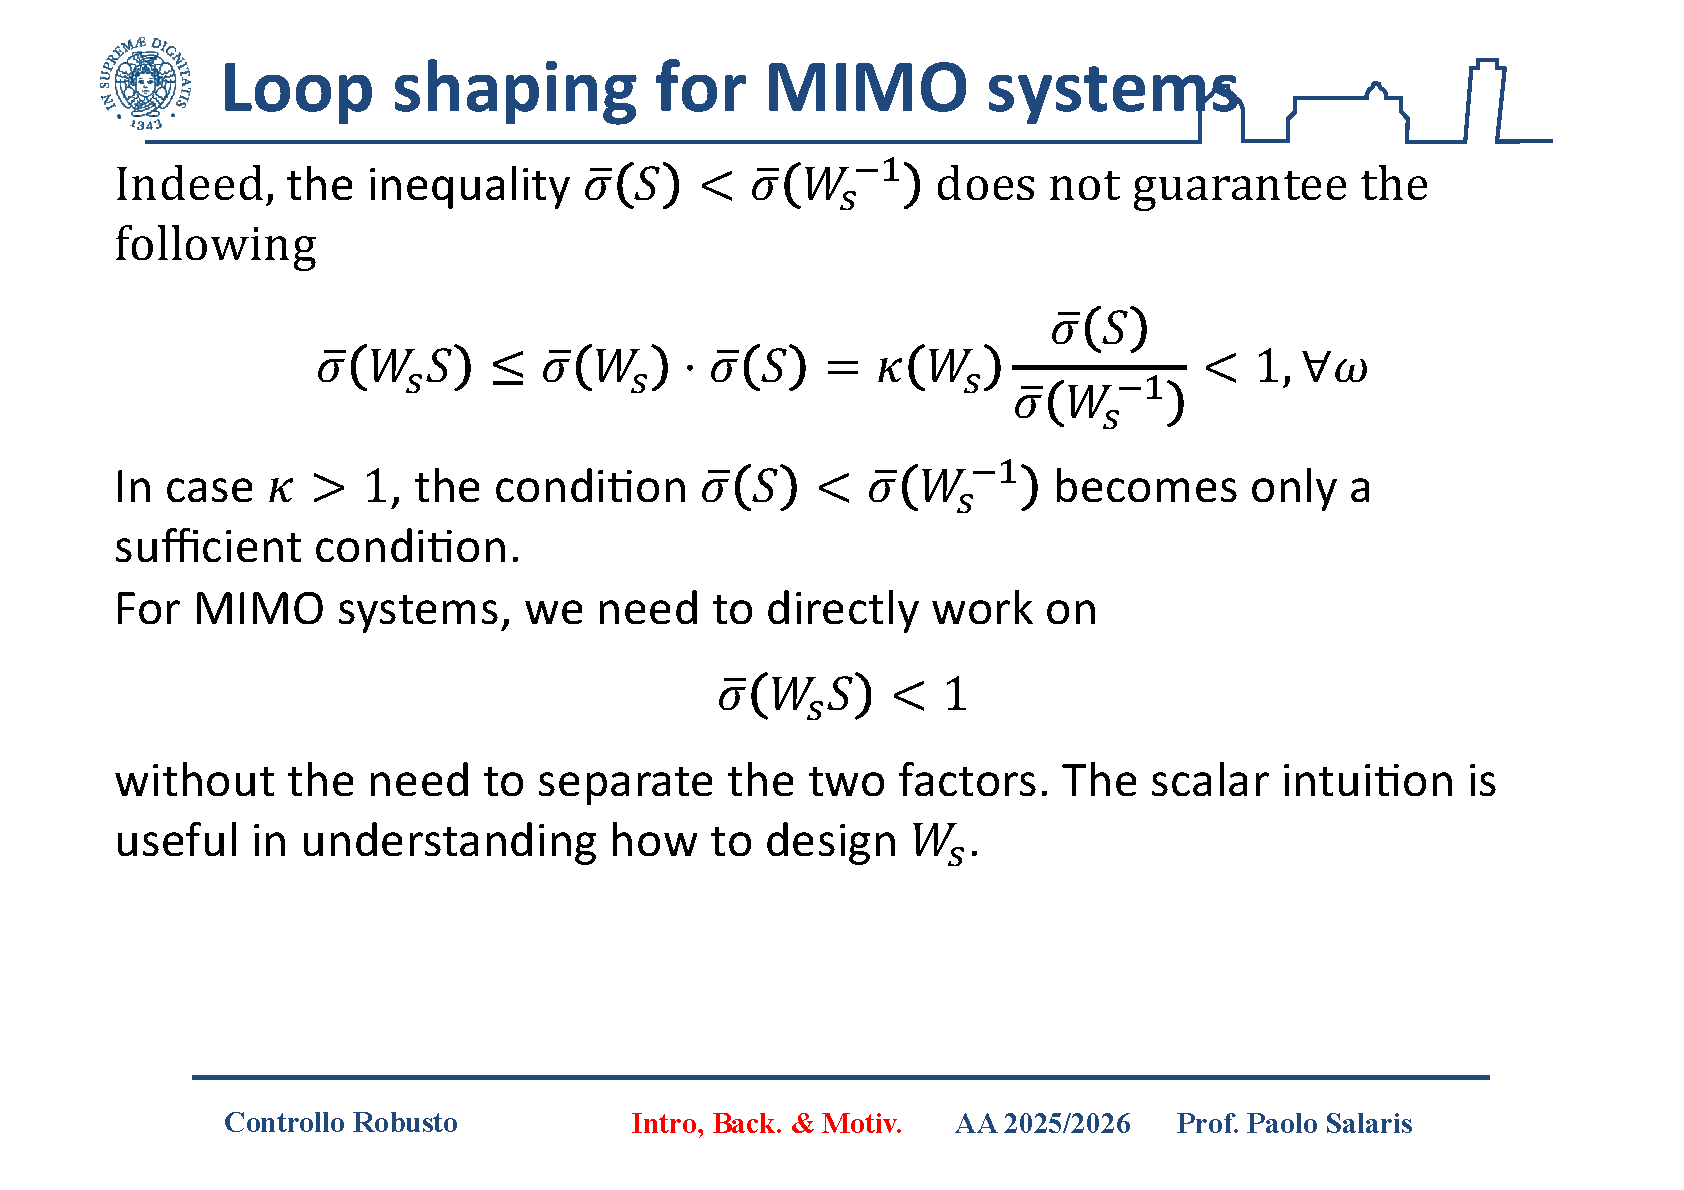
\includegraphics[width=\linewidth]{images4/slide-mimo-weights-002.png}
        \caption{Perché nel caso MIMO non basta confrontare separatamente $\bar{\sigma}(S_o)$ e $\bar{\sigma}(W_s^{-1})$.}
    \end{subfigure}
    \caption{Le slide 110 e 111 chiariscono che la specifica di prestazione va formulata sul prodotto $W_sS_o$, non sui fattori considerati isolatamente.}
\end{figure}

Il punto sottile, e qui si annidava anche un potenziale errore di interpretazione, è il seguente:
$$
\bar{\sigma}(W_s S_o)<1
\quad \Longrightarrow \quad
\bar{\sigma}(S_o)<\bar{\sigma}(W_s^{-1}),
$$
perché
$$
S_o=W_s^{-1}(W_sS_o)
\quad\Longrightarrow\quad
\bar{\sigma}(S_o)
\le
\bar{\sigma}(W_s^{-1})\,\bar{\sigma}(W_sS_o).
$$
Ma il viceversa in generale \emph{non} vale. Infatti dalla sola disuguaglianza
$$
\bar{\sigma}(S_o)<\bar{\sigma}(W_s^{-1})
$$
si può solo scrivere
$$
\bar{\sigma}(W_sS_o)
\le
\bar{\sigma}(W_s)\,\bar{\sigma}(S_o)
<
\bar{\sigma}(W_s)\,\bar{\sigma}(W_s^{-1})
=\kappa(W_s),
$$
che non garantisce affatto un valore minore di $1$ quando $\kappa(W_s)>1$. Il confronto fra $\bar{\sigma}(S_o)$ e $\bar{\sigma}(W_s^{-1})$ è quindi una condizione necessaria, non sufficiente, salvo il caso particolare $\kappa(W_s)=1$.

Se si vuole una condizione semplice ma conservativa, allora si può usare
$$
\bar{\sigma}(S_o)<\frac{1}{\bar{\sigma}(W_s)}
=\underline{\sigma}(W_s^{-1}),
$$
che garantisce
$$
\bar{\sigma}(W_sS_o)
\le
\bar{\sigma}(W_s)\bar{\sigma}(S_o)<1,
$$
ma al prezzo di perdere l'informazione direzionale contenuta nel peso.

La terza slide completa il quadro spiegando il ruolo di $W_t$. Il peso $W_t$ non descrive la direzione dell'incertezza, ma la sua \emph{taglia ammessa} alle diverse frequenze: quanto più $W_t$ è grande, tanto più stiamo dichiarando che l'errore di modello può essere severo in quella banda. La matrice normalizzata $\tilde{\Delta}$ cattura invece la forma direzionale dell'errore, con il vincolo $\bar{\sigma}(\tilde{\Delta})<1$. In questo linguaggio, progettare robustamente significa chiedere che il chiuso resti stabile per \emph{ogni} perturbazione compatibile con l'inviluppo fissato da $W_t$.

\begin{figure}[H]
    \centering
    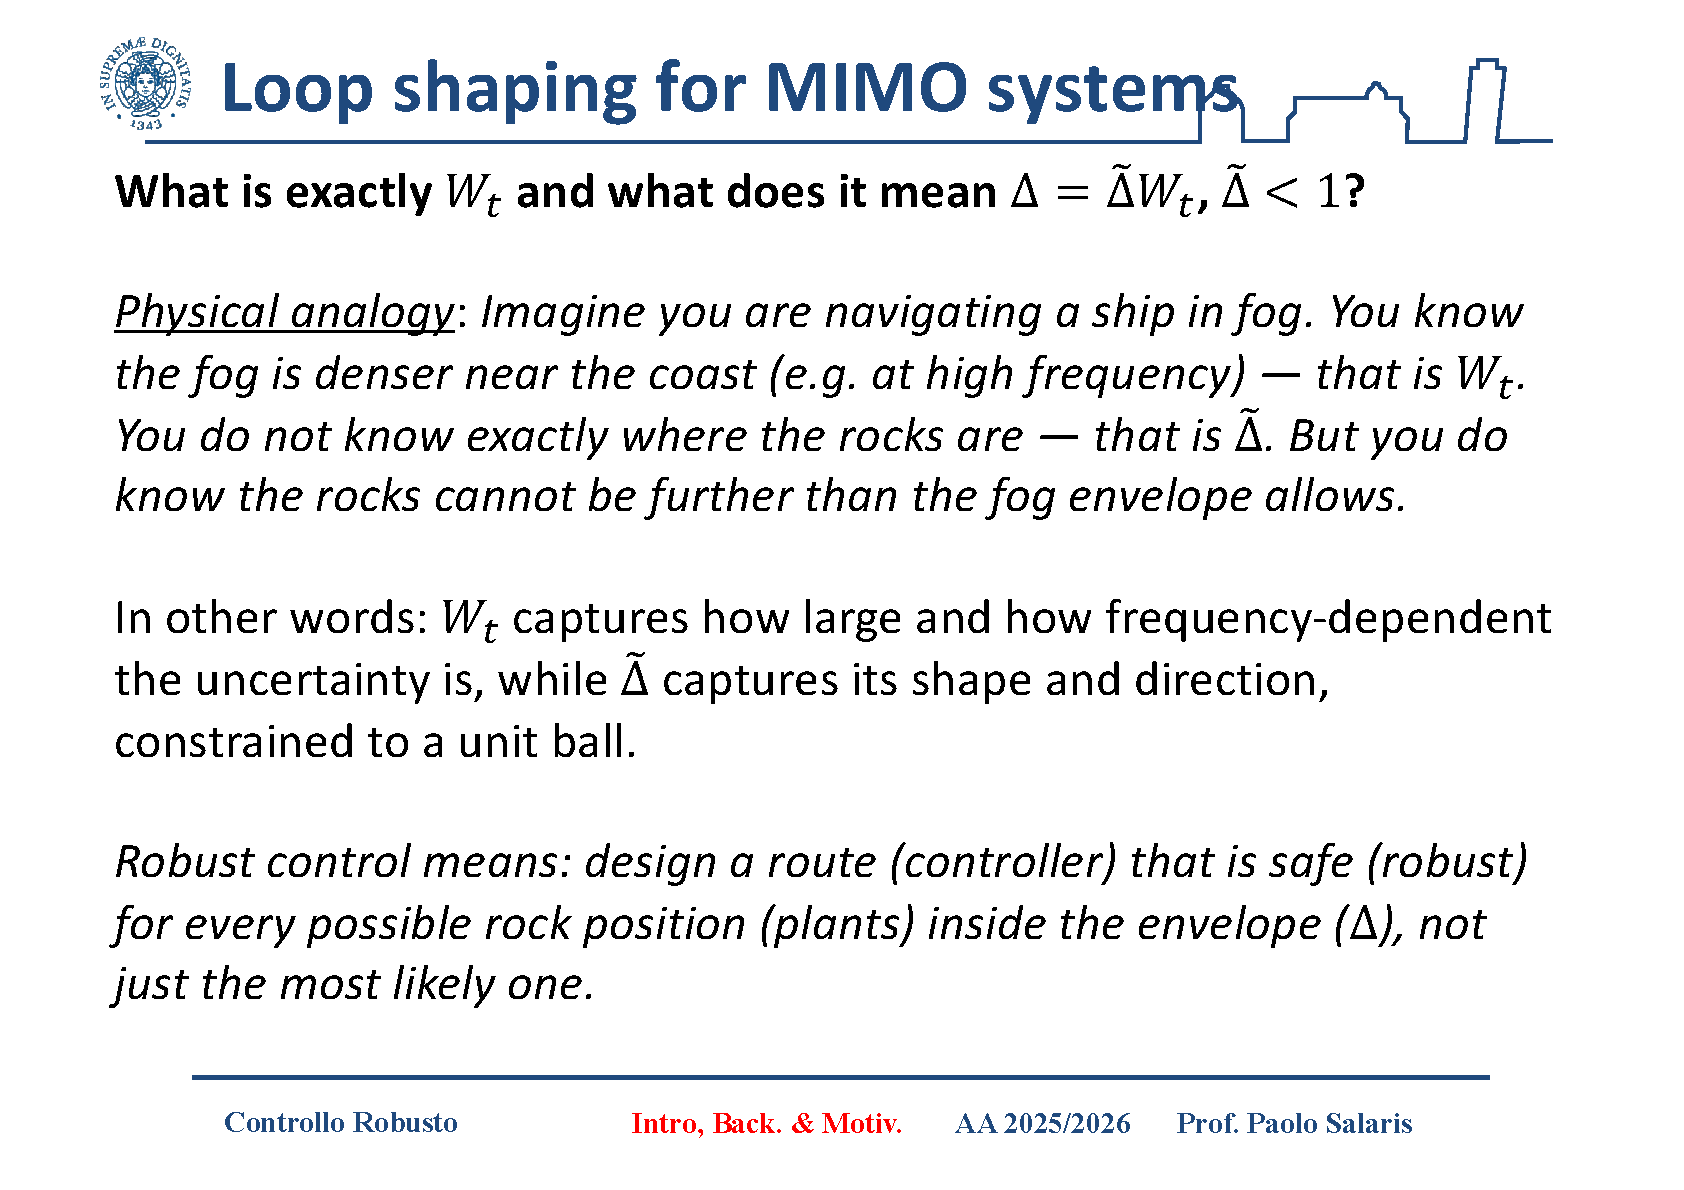
\includegraphics[width=0.78\textwidth]{images4/slide-mimo-weights-003.png}
    \caption{La slide 112 interpreta $W_t$ come inviluppo frequenziale dell'incertezza e $\tilde{\Delta}$ come sua forma direzionale normalizzata.}
\end{figure}

\begin{focusbox}
\textbf{Messaggio operativo.} Nel caso MIMO i pesi $W_s$ e $W_t$ non sono semplici curve da confrontare punto per punto con i moduli di $S_o$ e $T_o$. Sono matrici che selezionano direzioni e bande di frequenza. Perciò le specifiche corrette sono quelle sui prodotti pesati $W_sS_o$ e $W_tT_o$; ogni loro riduzione a bound scalari sul solo loop gain è comoda, ma inevitabilmente conservativa.
\end{focusbox}

\subsection{Architetture SISO a uno e due gradi di libertà}

\subsubsection{Controllo a un grado di libertà}

Le slide ritornano poi al caso SISO per mettere a fuoco la struttura di progetto più comune. Per coerenza con il materiale originale, in questa parte indichiamo con $G_d$ il canale del disturbo e con
$$
e = y-r
$$
l'errore di tracking, pur sapendo che in molta letteratura si usa la convenzione opposta $e=r-y$. Nel controllo a un grado di libertà si usa
$$
u = K(s)\bigl(r-y-n\bigr),
$$
e si chiede che l'errore resti piccolo nonostante il disturbo $d$ che entra attraverso $G_d$. Indicando con
$$
T = \frac{GK}{1+GK},
\qquad
S = \frac{1}{1+GK},
$$
l'uscita può essere scritta come
$$
y
= (1+GK)^{-1}GKr
+(1+GK)^{-1}G_d d
-(1+GK)^{-1}GKn,
$$
cioè, in forma compatta,
$$
y = T r + S G_d d - T n,
$$
e quindi
$$
e = y-r = S(G_d d-r) - T n.
$$

Questa decomposizione è molto istruttiva. Il riferimento compare nell'errore come $-Sr$, il disturbo compare come $SG_d d$, mentre il rumore di misura compare come $-Tn$. Di conseguenza, nel controllo a un solo grado di libertà tracking e rigetto dei disturbi sono accoppiati: per ridurre l'effetto di $d$ bisogna rendere piccolo lo stesso oggetto, $S$, che determina anche l'errore sul riferimento. Questo è comodo quando le due richieste sono compatibili, ma diventa limitante quando si vorrebbe una risposta al riferimento dolce e, contemporaneamente, un rigetto del disturbo molto aggressivo.

\begin{figure}[H]
    \centering
    \begin{subfigure}{0.48\textwidth}
        
\includegraphics[width=\linewidth]{images4/slide-14.png}
        \caption{Schema e decomposizione del caso a un grado di libertà.}
    \end{subfigure}
    \hfill
    \begin{subfigure}{0.48\textwidth}
        
\includegraphics[width=\linewidth]{images4/slide-15.png}
        \caption{Passaggio al controllo a due gradi di libertà.}
    \end{subfigure}
    \caption{Con una sola via di controllo tracking e rigetto dei disturbi sono accoppiati; la struttura a due gradi di libertà prova a separarli.}
\end{figure}

\subsubsection{Controllo a due gradi di libertà}

Per ridurre questo accoppiamento, la lezione introduce la struttura a due gradi di libertà:
$$
u = K(r-y-n) + K_r r - K_d d.
$$
Il blocco di feedback $K$ resta responsabile della stabilità, della robustezza e della sensitività; i blocchi addizionali $K_r$ e $K_d$ servono invece a modellare più finemente il canale del riferimento e quello del disturbo.

Le slide scrivono l'uscita nella forma
$$
y = (1+GK)^{-1}\Bigl(G(K+K_r)r + (G_d-GK_d)d - GKn\Bigr),
$$
e introducono grandezze ausiliarie che consentono di leggere separatamente il peso del riferimento e del disturbo. Ponendo
$$
S = (1+GK)^{-1},
\qquad
T = \frac{GK}{1+GK},
$$
e, quando $G_d$ è invertibile nella banda di interesse,
$$
S_r = 1-GK_r,
\qquad
S_d = 1-GK_dG_d^{-1},
$$
si ottiene
$$
e = y-r = -SS_r\,r + SS_d\,G_d d - Tn.
$$
Questa formula è molto più informativa della sola equazione dell'uscita, perché separa con chiarezza i tre contributi:
\begin{itemize}
    \item per migliorare il tracking si vuole rendere piccolo il prodotto $SS_r$;
    \item per migliorare il rigetto dei disturbi si vuole rendere piccolo il prodotto $SS_d$;
    \item tali obiettivi possono essere sagomati parzialmente in modo indipendente grazie ai rami aggiuntivi $K_r$ e $K_d$.
\end{itemize}

Da un punto di vista robusto, la distinzione è preziosa. Il feedback principale $K$ viene progettato per garantire stabilità interna e insensibilità alle incertezze; i rami addizionali $K_r$ e $K_d$ servono invece a rifinire il comportamento nominale, senza dover caricare tutto il compromesso prestazione/robustezza sul solo loop principale.

\begin{keybox}
La struttura a due gradi di libertà non sostituisce il feedback: lo alleggerisce. $K$ deve ancora costruire un loop robusto; $K_r$ e $K_d$ servono a sagomare meglio riferimento e disturbo quando il modello nominale è abbastanza affidabile.
\end{keybox}

\subsubsection{Perché il feed-forward da solo non basta}

Le slide successive mostrano una situazione-limite: si elimina il feedback e si prova a compensare tutto in feed-forward con
$$
u = K_r r - K_d d.
$$
Se il modello fosse perfetto, si potrebbe scegliere idealmente
$$
K_r(s)=G^{-1}(s),
\qquad
K_d(s)=G^{-1}(s)G_d(s),
$$
ottenendo cancellazione esatta del processo e del disturbo. Ma questo scenario è proprio ciò che nella pratica non si verifica mai in modo affidabile.

La formula da tenere in mente è
$$
y = G K_r r + (G_d-GK_d)d.
$$
Con
$$
K_r=G^{-1},
\qquad
K_d=G^{-1}G_d,
$$
si avrebbe formalmente $y=r$ e cancellazione del disturbo. Questa però è un'inversione esplicita del processo, quindi eredita tutte le fragilità del modello.

I motivi elencati nelle slide sono tre:
\begin{enumerate}
    \item incertezza di segnale, cioè disturbi non noti con esattezza;
    \item incertezza di modello, cioè impossibilità di realizzare l'inverso esatto del processo reale;
    \item eventuale instabilità del processo, che rende l'inversione diretta inutilizzabile o non causale.
\end{enumerate}

Il feedback serve esattamente a superare questi limiti. Se infatti il loop gain è grande,
$$
L = GK \gg 1,
$$
allora
$$
S = (1+GK)^{-1} \approx 0,
\qquad
T = 1-S \approx 1.
$$
Ne segue che
$$
y = Tr + SG_d d - Tn \approx r-n,
$$
mentre il comando può essere riscritto come
$$
u = KSr - KSG_d d - KSn
=
KS(r-G_d d-n).
$$
Usando l'identità
$$
KS = G^{-1}T,
$$
si ottiene allora, in regime di alto guadagno dove $T\approx 1$,
$$
u \approx G^{-1}(r-G_d d-n).
$$
Cioè il feedback ricostruisce in modo implicito l'inverso del processo senza richiedere un modello perfetto esplicito. La slide finale di questo blocco ricorda però il rovescio della medaglia: un \emph{high gain} spinto senza criterio può degradare i margini e perfino indurre instabilità.

\begin{figure}[H]
    \centering
    \begin{subfigure}{0.48\textwidth}
        
\includegraphics[width=\linewidth]{images4/slide-16.png}
        \caption{Compensazione puramente feed-forward e sue fragilità strutturali.}
    \end{subfigure}
    \hfill
    \begin{subfigure}{0.48\textwidth}
        
\includegraphics[width=\linewidth]{images4/slide-17.png}
        \caption{Beneficio del feedback ad alto guadagno: l'inversione del processo emerge in modo implicito.}
    \end{subfigure}
    \caption{Il confronto fra feed-forward puro e feedback mostra perché, in presenza di incertezza, la retroazione resti indispensabile.}
\end{figure}

\subsection{Stabilità in anello chiuso e guadagno ultimo}

La parte finale della lezione torna su un esempio SISO per legare le idee di loop shaping ai concetti classici di stabilità. Il processo considerato è
$$
G(s)=\frac{3(-2s+1)}{(10s+1)(5s+1)},
$$
che possiede uno zero nel semipiano destro in
$$
s = 0.5 \ \text{rad/s}.
$$
Si considera quindi una retroazione con guadagno proporzionale $K_c$ e si studia la stabilità del chiuso.

Scrivendo l'equazione caratteristica
$$
1 + K_c G(s) = 0,
$$
si ottiene
$$
(10s+1)(5s+1) + 3K_c(-2s+1)=0,
$$
cioè
$$
50s^2 + (15-6K_c)s + (1+3K_c)=0.
$$
Poiché il polinomio è del secondo ordine, la stabilità richiede semplicemente che i coefficienti siano positivi, da cui
$$
15-6K_c > 0,
\qquad
1+3K_c > 0.
$$
Ne segue
$$
-\frac{1}{3} < K_c < 2.5.
$$
Con retroazione negativa interessa il caso $K_c>0$, quindi la regione utile è
$$
0 < K_c < 2.5.
$$
Questo passaggio è importante perché traduce una lettura qualitativa del grafico temporale in una condizione analitica precisa: aumentando $K_c$ si riduce l'errore statico, ma si spostano anche i poli chiusi; quando $K_c$ arriva a $2.5$, il coefficiente del termine in $s$ si annulla e i poli finiscono sull'asse immaginario.

Il valore
$$
K_u = 2.5
$$
è il \emph{guadagno ultimo}: per questo valore il sistema si porta al bordo della stabilità e, come mostrato nella slide, compaiono oscillazioni persistenti con periodo circa
$$
P_u \approx 15.2 \ \text{s},
$$
corrispondente a una frequenza di circa
$$
\omega_u \approx 0.42 \ \text{rad/s}.
$$

\begin{figure}[H]
    \centering
    \begin{subfigure}{0.48\textwidth}
        
\includegraphics[width=\linewidth]{images4/slide-18.png}
        \caption{Risposta temporale per diversi valori del guadagno proporzionale.}
    \end{subfigure}
    \hfill
    \begin{subfigure}{0.48\textwidth}
        
\includegraphics[width=\linewidth]{images4/slide-19.png}
        \caption{Verifica analitica e frequenziale della soglia di stabilità.}
    \end{subfigure}
    \caption{L'esempio con zero nel semipiano destro mostra come il limite sul guadagno ammissibile possa essere letto sia dal polinomio caratteristico sia dalla risposta in frequenza.}
\end{figure}

La stessa conclusione si ricava infatti nel dominio della frequenza. Alla frequenza in cui la fase di $L(j\omega)$ vale $-180^\circ$, il criterio di Nyquist richiede
$$
|L(j\omega_{180})|<1.
$$
Nel caso in esame la slide mostra che
$$
|L(j\omega_{180})| = 0.4\,K_c,
$$
da cui di nuovo
$$
0.4\,K_c < 1
\quad \Longrightarrow \quad
K_c < 2.5.
$$
Questo è un collegamento molto didattico: la stessa soglia emerge sia da una condizione sui poli chiusi, sia dalla lettura geometrica della risposta in frequenza.

\begin{focusbox}
\textbf{Lettura fisica del guadagno ultimo.} $K_u$ non è un buon guadagno di progetto: è il guadagno al limite dell'instabilità. Serve come informazione sperimentale per capire dove si trova il bordo, non come valore da usare direttamente in un controllore robusto.
\end{focusbox}

\subsection{Margini di stabilità e loro significato fisico}

Una volta ottenuto un sistema chiuso stabile, le slide introducono i \emph{margini di stabilità}, cioè misure quantitative della distanza del sistema dall'instabilità. Nel caso SISO, i due margini classici sono
$$
GM = \frac{1}{|L(j\omega_{180})|},
\qquad
\angle L(j\omega_{180}) = -180^\circ,
$$
e
$$
PM = \angle L(j\omega_c) + 180^\circ,
\qquad
|L(j\omega_c)|=1.
$$

Il margine di guadagno $GM$ misura quanto si può aumentare il guadagno dell'anello prima di raggiungere il punto critico $-1$. È quindi una protezione diretta contro errori sul guadagno statico del modello. Il margine di fase $PM$, invece, misura quanta ulteriore fase negativa può essere tollerata alla frequenza di crossover: per questo viene interpretato come un indicatore della tolleranza verso ritardi puri o dinamiche non modellate.

Le slide riportano anche due soglie pratiche molto note:
\begin{itemize}
    \item tipicamente si desidera $GM>2$;
    \item tipicamente si desidera $PM \ge 30^\circ$.
\end{itemize}
Inoltre, se $PM$ è espresso in radianti, il massimo ritardo puro tollerabile è approssimativamente
$$
\theta_{\max} \approx \frac{PM}{\omega_c}.
$$

\begin{figure}[H]
    \centering
    
\includegraphics[width=0.78\textwidth]{images4/slide-20.png}
    \caption{Definizione geometrica di margine di guadagno e margine di fase sul diagramma di Bode e nel piano di Nyquist.}
\end{figure}

\subsection{Osservazione critica sulla taratura di Ziegler--Nichols}

La slide successiva usa il processo precedente per ricordare che una taratura puramente empirica può essere lontana dalle esigenze del controllo robusto. Applicando la regola di Ziegler--Nichols per un PI,
$$
K_c = \frac{K_u}{2.2},
\qquad
T_i = \frac{P_u}{1.2},
$$
si ottiene un controllore del tipo
$$
K(s)=K_c\left(1+\frac{1}{T_i s}\right),
$$
con $K_u=2.5$ e $P_u \approx 15.25\,\text{s}$.
Numericamente,
$$
K_c=\frac{2.5}{2.2}\approx 1.136,
\qquad
T_i=\frac{15.25}{1.2}\approx 12.7\,\text{s},
$$
per cui
$$
K(s)\approx 1.136\left(1+\frac{1}{12.7s}\right).
$$

Il diagramma mostrato in slide evidenzia che i margini risultanti sono modesti:
\begin{itemize}
    \item il margine di fase è circa $19.4^\circ$, quindi inferiore al valore tipicamente desiderato;
    \item il margine di guadagno è circa $1.63$, anch'esso inferiore alla soglia pratica $2$;
    \item la frequenza di crossover è circa $\omega_c=0.236\,\text{rad/s}$;
    \item il ritardo massimo tollerabile è circa $\theta_{\max}=1.4\,\text{s}$;
    \item i picchi di sensitività risultano elevati, con valori dell'ordine di $M_s \approx 3.92$ e $M_t \approx 3.35$.
\end{itemize}

Il significato dell'esempio è molto chiaro: una taratura classica basata sul solo guadagno ultimo può produrre un sistema che magari funziona nominalmente, ma resta troppo vicino al bordo dell'instabilità e presenta un'amplificazione eccessiva di certe componenti di frequenza. Dal punto di vista robusto, quindi, non basta ``chiudere l'anello''; occorre anche controllare come il luogo di Nyquist e i diagrammi di Bode si dispongono rispetto ai vincoli di margine e ai picchi di sensitività.

\begin{figure}[H]
    \centering
    
\includegraphics[width=0.78\textwidth]{images4/slide-21.png}
    \caption{Esempio di PI tarato con Ziegler--Nichols: i margini risultano troppo piccoli e i picchi di sensitività troppo grandi per un progetto robusto convincente.}
\end{figure}

\subsection{Specifiche prestazionali in norma infinita}

L'ultima coppia di slide collega in modo elegante i margini di stabilità alle prestazioni del chiuso. Vengono introdotti i picchi
$$
M_s = \max_{\omega} |S(j\omega)| = \|S\|_\infty,
\qquad
M_t = \max_{\omega} |T(j\omega)| = \|T\|_\infty.
$$
Qui $\|\cdot\|_\infty$ è la norma in frequenza della funzione di trasferimento stabile: nel SISO coincide con il massimo modulo del diagramma di Bode, mentre nel MIMO diventerà il massimo, su $\omega$, del massimo valore singolare. Nel linguaggio del progetto robusto, $M_s$ misura il peggior caso di sensibilità del sistema chiuso, mentre $M_t$ misura il massimo picco della sensitività complementare. Valori grandi di queste quantità segnalano contemporaneamente cattiva prestazione e bassa robustezza; le slide ricordano come valori tipici desiderabili siano
$$
M_s < 2,
\qquad
M_t < 1.25.
$$

Queste grandezze hanno un significato molto diretto anche nel dominio del tempo. Senza feedback si avrebbe
$$
e = y-r = G_d d - r,
$$
mentre con feedback
$$
e = S(G_d d-r).
$$
Se quindi $|S(j\omega)|<1$ nelle frequenze in cui riferimento e disturbo sono importanti, l'errore chiuso viene ridotto rispetto al caso aperto. Se invece $|S(j\omega)|$ ha un picco elevato, vuol dire che esiste una banda in cui il feedback amplifica l'errore invece di attenuarlo. La norma infinita di $S$ fornisce allora una misura sintetica del peggior caso.

\begin{figure}[H]
    \centering
    \begin{subfigure}{0.48\textwidth}
        
\includegraphics[width=\linewidth]{images4/slide-22.png}
        \caption{Definizione dei picchi $M_s$ e $M_t$ e loro interpretazione prestazionale.}
    \end{subfigure}
    \hfill
    \begin{subfigure}{0.48\textwidth}
        
\includegraphics[width=\linewidth]{images4/slide-23.png}
        \caption{Dimostrazione del legame fra margini di stabilità e valori massimi di $S$ e $T$.}
    \end{subfigure}
    \caption{Le norme di $S$ e $T$ trasformano i margini di stabilità in vere e proprie specifiche di prestazione chiusa.}
\end{figure}

\subsubsection{Legame con il margine di guadagno}

Alla frequenza $\omega_{180}$, per definizione del margine di guadagno vale
$$
L(j\omega_{180}) = -\frac{1}{GM}.
$$
Sostituendo in
$$
S = \frac{1}{1+L},
\qquad
T = \frac{L}{1+L},
$$
si ricava
$$
S(j\omega_{180}) = \frac{GM}{GM-1},
\qquad
T(j\omega_{180}) = -\frac{1}{GM-1}.
$$
Prendendo i moduli e ricordando che $M_s$ e $M_t$ sono massimi su tutte le frequenze, si ottiene
$$
M_s \ge \frac{GM}{GM-1},
\qquad
M_t \ge \frac{1}{GM-1}.
$$
Queste disuguaglianze vanno lette nel verso giusto. Dato un sistema, il picco $M_s$ non può essere più piccolo del valore assunto da $|S|$ alla frequenza di fase $-180^\circ$; lo stesso vale per $M_t$. Se in fase di progetto imponiamo un limite superiore a $M_s$ e $M_t$, allora otteniamo automaticamente margini minimi:
$$
M_s^{\max} \ge \frac{GM}{GM-1}
\quad\Longrightarrow\quad
GM \ge \frac{M_s^{\max}}{M_s^{\max}-1},
$$
e
$$
M_t^{\max} \ge \frac{1}{GM-1}
\quad\Longrightarrow\quad
GM \ge 1+\frac{1}{M_t^{\max}}.
$$
Usando, come nelle slide, la stessa lettera per il limite ammesso e per il valore massimo misurato, si scrive più sinteticamente
$$
GM \ge \frac{M_s}{M_s-1},
\qquad
GM \ge 1+\frac{1}{M_t}.
$$

\subsubsection{Legame con il margine di fase}

Alla frequenza di crossover $\omega_c$, dove $|L(j\omega_c)|=1$, la geometria nel piano complesso mostra che la distanza del punto $L(j\omega_c)$ dal punto critico $-1$ è
$$
|1+L(j\omega_c)| = 2\sin\!\left(\frac{PM}{2}\right).
$$
Di conseguenza
$$
|S(j\omega_c)|
=
|T(j\omega_c)|
=
\frac{1}{2\sin(PM/2)}.
$$
Ancora una volta, essendo $M_s$ e $M_t$ massimi globali, segue che
$$
M_s \ge \frac{1}{2\sin(PM/2)},
\qquad
M_t \ge \frac{1}{2\sin(PM/2)}.
$$
Risolvendo rispetto a $PM$ si ottengono stime inferiori molto utili:
$$
PM \ge 2\arcsin\!\left(\frac{1}{2M_s}\right),
\qquad
PM \ge 2\arcsin\!\left(\frac{1}{2M_t}\right).
$$
Anche qui la lettura corretta è progettuale: limitare i picchi di $S$ e $T$ impedisce al Nyquist di passare troppo vicino al punto critico $-1$, e quindi impone un margine di fase minimo.

\subsubsection{Valori pratici}

Le slide chiudono con due esempi numerici molto usati in pratica. Se si sceglie
$$
M_s = 2,
$$
allora dalle formule precedenti si ricava
$$
GM \ge 2,
\qquad
PM \ge 29^\circ.
$$
Se invece si impone
$$
M_t = 2,
$$
si ottiene
$$
GM \ge 1.5,
\qquad
PM \ge 29^\circ.
$$

Questi valori non vanno letti come equivalenze esatte, ma come regole di progetto conservative e molto utili. Mostrano che margini ``decenti'' e picchi moderati di sensitività sono due facce dello stesso problema: entrambi misurano quanto il sistema chiuso sia vicino a una risonanza eccessiva o a una perdita di robustezza.

\subsection{Sintesi conclusiva della lezione}

Questa lezione completa il passaggio dalla semplice analisi della stabilità alla progettazione robusta vera e propria. Il primo messaggio è che le prestazioni possono essere lette attraverso pochi canali fondamentali del sistema chiuso, governati da $S_o$, $T_o$, $S_i$ e $T_i$. In termini pratici, seguire bene il riferimento e rigettare i disturbi significa modellare opportunamente i guadagni principali di queste matrici nelle bande di frequenza rilevanti.

Il secondo messaggio è che il \emph{loop shaping} nasce precisamente da questo punto di vista. Non si progetta il controllore alla cieca: si sceglie prima quale forma debba avere il loop transfer per essere grande dove serve la prestazione e piccolo dove servono robustezza, filtraggio del rumore e moderazione del comando. Nel caso SISO ciò porta a una procedura molto trasparente; nel caso MIMO la stessa filosofia resta valida, ma occorre tenere conto della struttura direzionale del problema e dei limiti delle sovrastime scalari.

Il terzo messaggio è che margini di stabilità e picchi di sensitività non sono indicatori indipendenti, ma descrizioni complementari della stessa realtà. Un progetto robusto credibile deve quindi controllare simultaneamente forma del loop gain, margini di guadagno e di fase, valori di $M_s$ e $M_t$, e compatibilità del comando con i limiti fisici degli attuatori. È proprio questa visione unificata a trasformare il feedback da semplice strumento di stabilizzazione a vera tecnica di progetto robusto.

\clearpage
\phantomsection
\section*{Appendice}
\addcontentsline{toc}{section}{Appendice}

\subsection*{Nota terminologica sui guadagni principali}
\phantomsection
\addcontentsline{toc}{subsection}{Nota terminologica sui guadagni principali}

Nelle slide l'espressione \emph{principal gains} coincide, nel caso MIMO, con i valori singolari della matrice di trasferimento. Il massimo valore singolare $\bar{\sigma}$ descrive il massimo guadagno ottenibile scegliendo la direzione di ingresso più sfavorevole, mentre il minimo valore singolare $\underline{\sigma}$ descrive la direzione meno amplificata. Per questo le specifiche MIMO non possono essere riassunte da un solo modulo scalare: bisogna distinguere sempre tra direzioni forti e direzioni deboli del sistema.

\subsection*{Riferimento al materiale originale}
\phantomsection
\addcontentsline{toc}{subsection}{Riferimento al materiale originale}

Questa parte del documento è una traduzione e rielaborazione estesa del blocco di slide del corso di Controllo Robusto A.A. 2025/2026 dedicato a ``principal gains'', ``loop shaping'' e ``closed-loop performance specifications'', caricato dall'utente come materiale di partenza.

\begin{coverpage}
\centering
{\Huge\bfseries Controllo Robusto\par}
\vspace{0.4em}
{\LARGE Traduzione in italiano e approfondimento\par}
\vspace{0.5em}
{\Large Norme per vettori e segnali, Parseval e residui\par}
\vfill

\includegraphics[width=0.78\textwidth]{images5/norms-01x-001.png}
\vfill
\begin{focusbox}
\textbf{Obiettivo del documento.} Questa parte del testo apre la Lezione 6 con una breve chiusura del blocco sul \emph{loop shaping} SISO e poi introduce il linguaggio delle norme per vettori e segnali. Il punto chiave è che grandezze come $M_s=\|S\|_\infty$ e $M_t=\|T\|_\infty$, già incontrate nella Lezione 5, non sono dettagli notazionali: sono il primo segnale del fatto che il controllo robusto ragiona naturalmente in termini di norme. Per questo la lezione passa dalle specifiche in frequenza alle norme $\ell_p$ e $L_2$, al teorema di Parseval e al calcolo della norma tramite il teorema dei residui.
\end{focusbox}
\vfill
{\large Basato sulle slide del corso AA 2025/2026\par}
\end{coverpage}

\section{Lezione 6}

\subsection{Visione d'insieme della lezione}

La Lezione 6 ha una struttura leggermente diversa dalle precedenti, ma molto istruttiva. Le prime quattro slide richieste dal PDF introduttivo non aprono un capitolo completamente nuovo: chiudono invece in modo più compatto il ragionamento della Lezione 5. Riassumono il significato di $M_s$ e $M_t$, mostrano come tali quantità siano già norme $H_\infty$ dei canali chiusi, e propongono un primo esempio di scelta della forma desiderata del loop transfer $L(s)$. In questo senso funzionano come ponte: fanno vedere che la progettazione robusta non si esprime solo con parole come ``banda'' o ``margine'', ma con misure quantitative ben precise della grandezza di segnali e operatori.

Da qui la lezione entra nel nuovo capitolo sulle norme. Si parte dalle norme di vettori, perché sono il modello più semplice di ciò che significa misurare la grandezza di un oggetto matematico in modo coerente. Poi si passa ai segnali nel tempo continuo e si introduce la norma $L_2$, che ha una lettura fisica immediata in termini di energia. Il passo successivo è il collegamento tra dominio del tempo e dominio della frequenza tramite il teorema di Parseval, seguito da una tecnica molto utile in controllo: il calcolo della norma mediante il teorema dei residui.

Le ultime slide del blocco mostrano due esempi semplici ma molto formativi. In entrambi i casi si calcola la norma $L_2$ dello stesso segnale in due modi diversi: direttamente nel tempo e poi nel dominio di Laplace usando i residui. Il messaggio da trattenere non è soltanto il risultato numerico, ma il metodo: in controllo robusto si passa continuamente da rappresentazioni temporali, frequenziali e complesse della stessa quantità, scegliendo di volta in volta quella più comoda da usare.

\begin{keybox}
La lezione contiene un messaggio unificante molto forte: le specifiche di prestazione e robustezza non sono altro che richieste sul fatto che certi segnali o certi operatori restino ``piccoli'' in un senso matematico appropriato. Le norme servono precisamente a dare forma rigorosa a questa idea.
\end{keybox}

\subsection{Ponte dalla Lezione 5: specifiche chiuse e forma desiderata del loop}

Le prime due slide riprendono il risultato conclusivo della Lezione 5 e lo condensano in una forma molto operativa. Le quantità
$$
M_s=\max_\omega |S(j\omega)|=\|S\|_\infty,
\qquad
M_t=\max_\omega |T(j\omega)|=\|T\|_\infty,
$$
non sono semplicemente due indici empirici: sono i picchi massimi della sensibilità e della sensibilità complementare. Per questo rappresentano una misura diretta della peggiore amplificazione che il sistema chiuso può produrre.

La slide richiama anche il loro significato fisico. Se l'errore chiuso è
$$
e = S(G_d d-r),
$$
allora nelle bande in cui $|S(j\omega)|<1$ il feedback migliora davvero il comportamento rispetto al caso senza controllo. Valori grandi di $M_s$ o di $M_t$ segnalano invece un sistema che, in qualche intervallo di frequenze, amplifica eccessivamente errori, disturbi o rumore, cioè un sistema insieme poco robusto e poco ``ben smorzato''.

La seconda slide rende questo quadro ancora più preciso collegando $M_s$ e $M_t$ ai margini classici. Le relazioni
$$
GM \ge \frac{M_s}{M_s-1},
\qquad
GM \ge 1+\frac{1}{M_t},
$$
e
$$
PM \ge 2\arcsin\!\left(\frac{1}{2M_s}\right),
\qquad
PM \ge 2\arcsin\!\left(\frac{1}{2M_t}\right),
$$
mostrano che margini di stabilità e picchi di sensitività non sono due linguaggi diversi, ma due modi di misurare la stessa distanza del sistema chiuso dal comportamento critico.

\begin{figure}[H]
    \centering
    \begin{subfigure}{0.48\textwidth}
        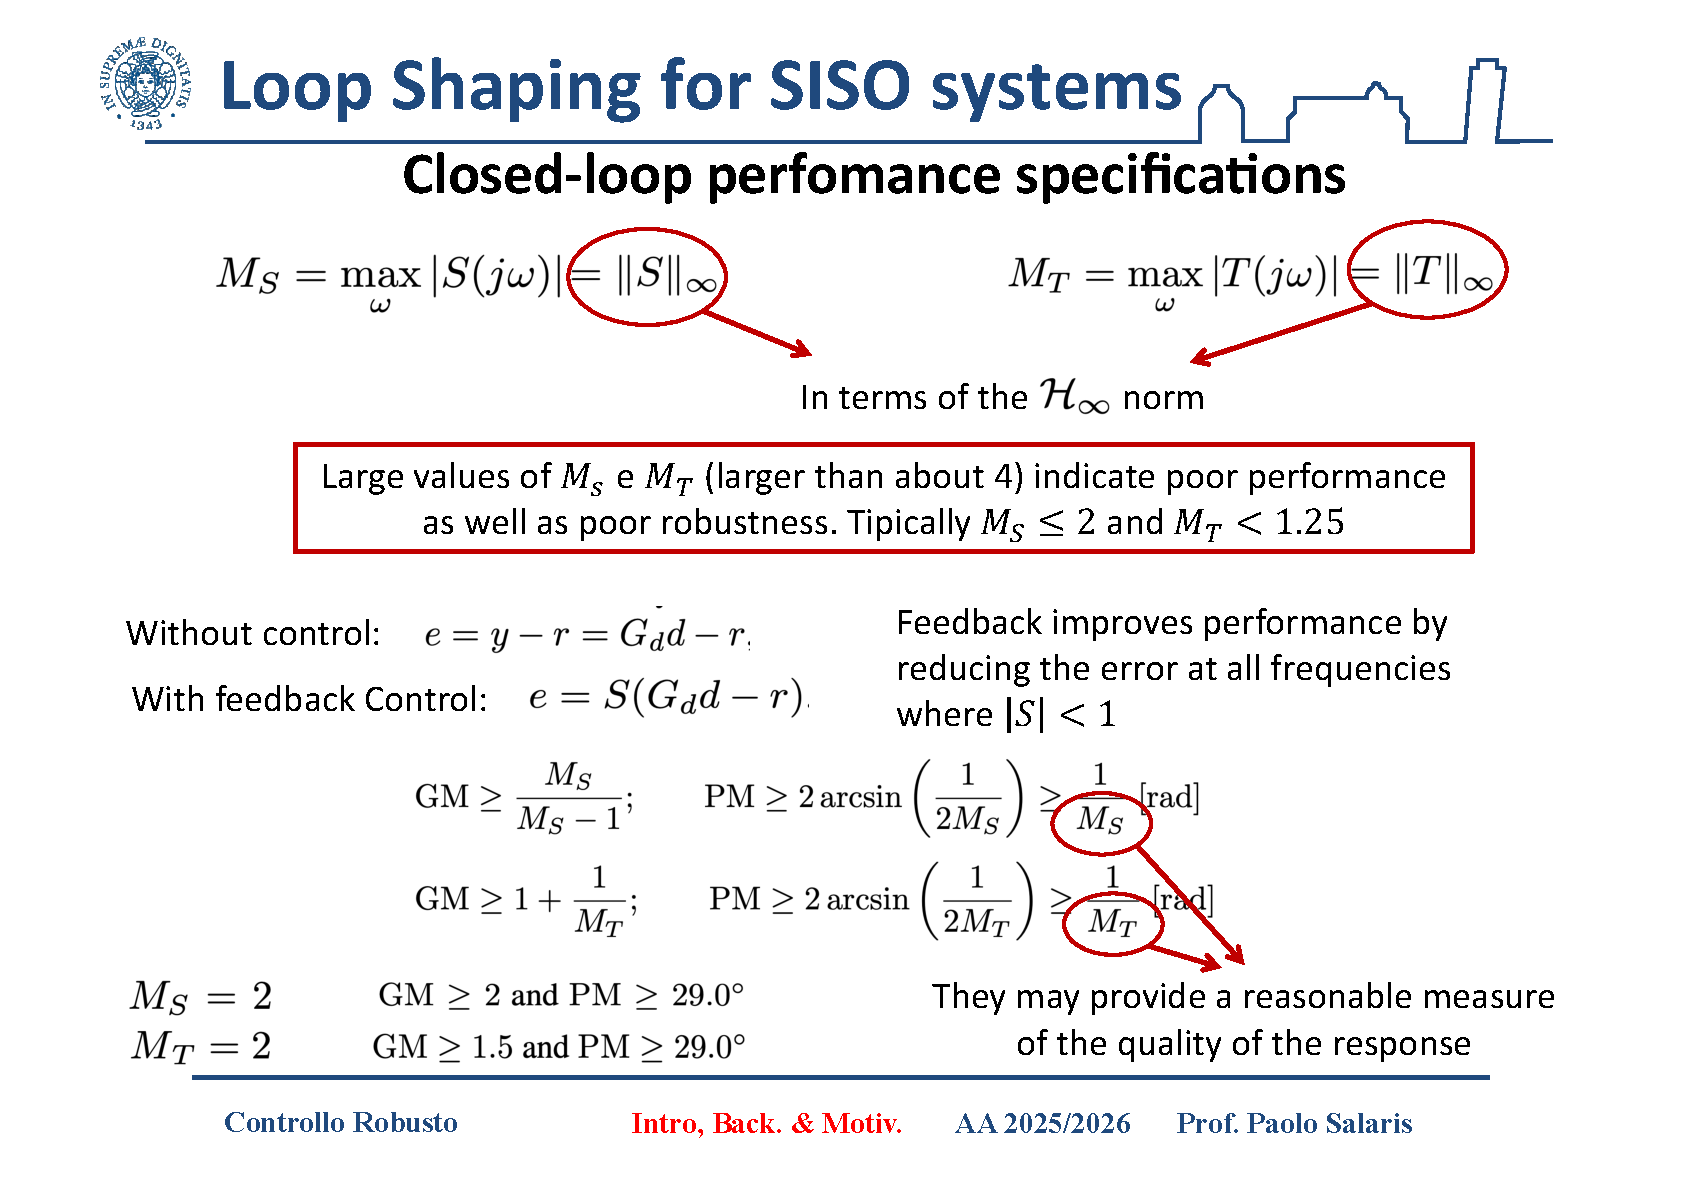
\includegraphics[width=\linewidth]{images5/intro-12x-001.png}
        \caption{Sintesi delle specifiche chiuse espresse tramite $M_s=\|S\|_\infty$ e $M_t=\|T\|_\infty$.}
    \end{subfigure}
    \hfill
    \begin{subfigure}{0.48\textwidth}
        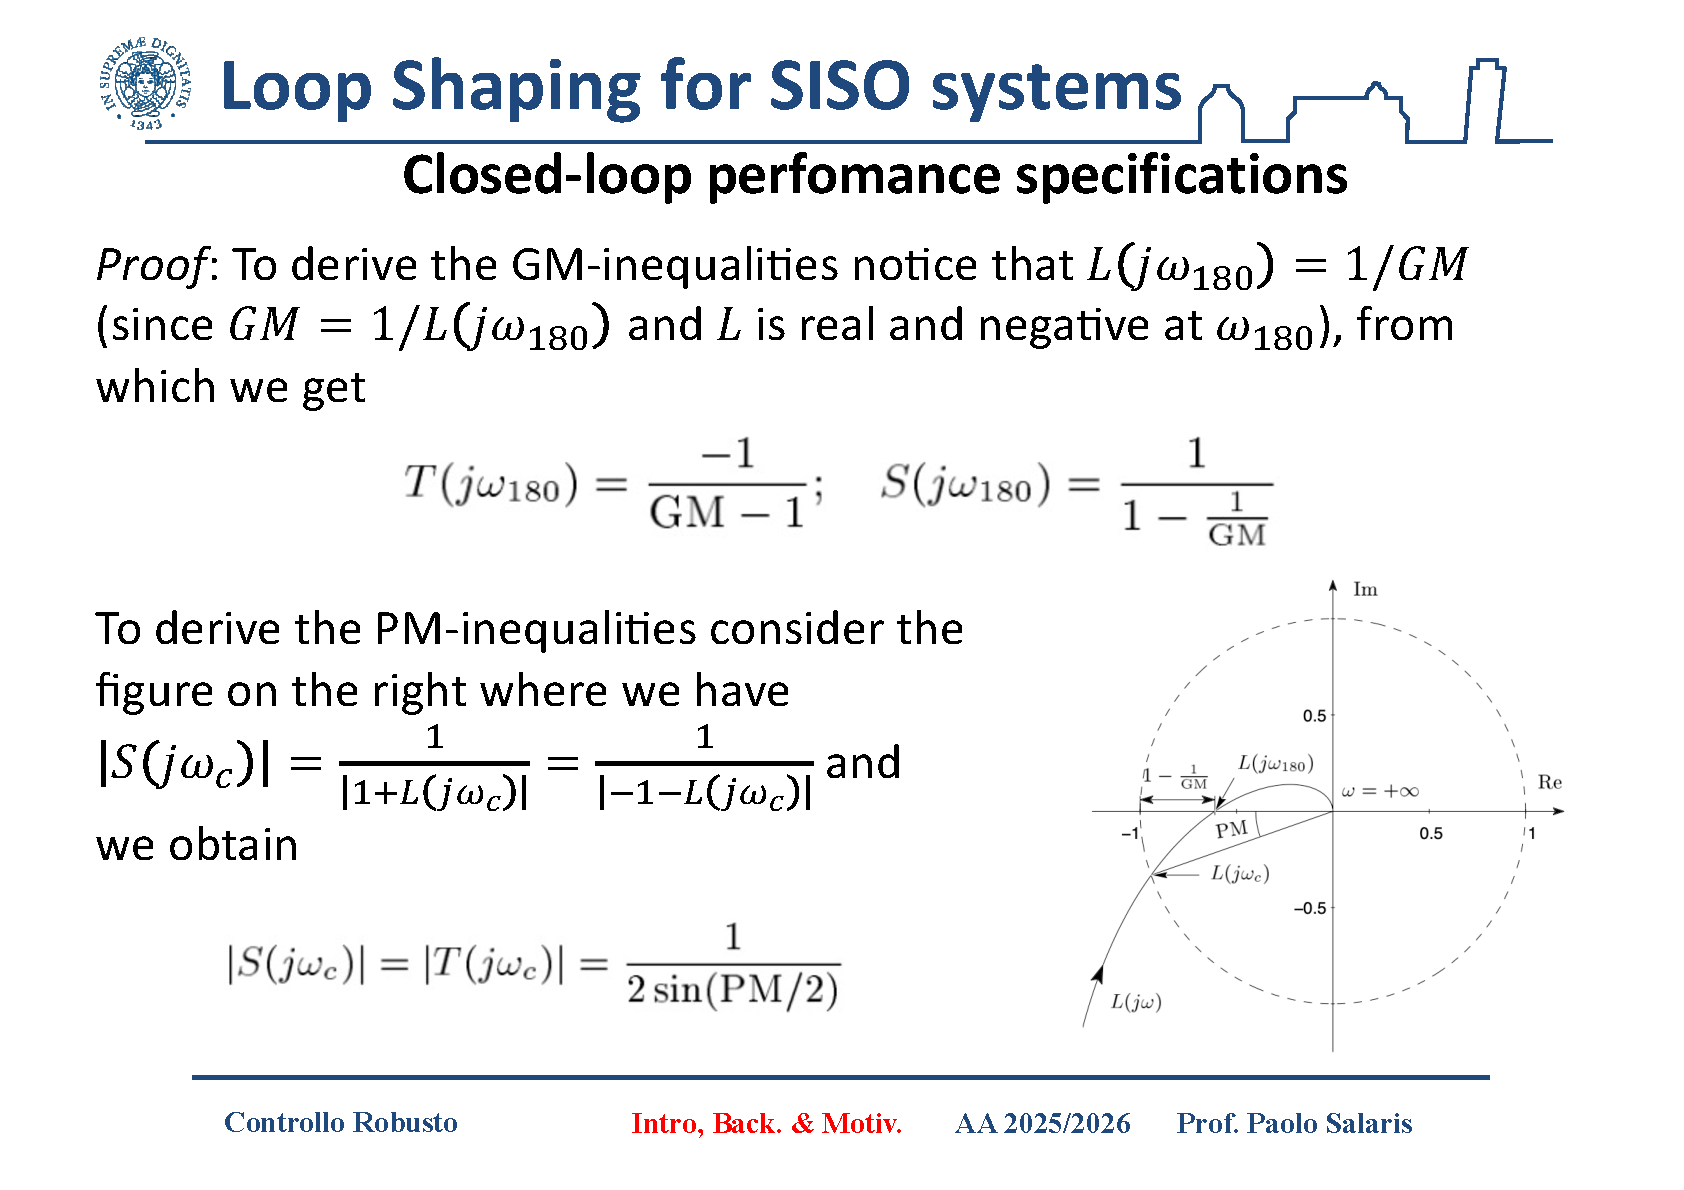
\includegraphics[width=\linewidth]{images5/intro-12x-002.png}
        \caption{Dimostrazione del legame fra norme di sensitività e margini classici di guadagno e fase.}
    \end{subfigure}
    \caption{Le ultime slide del PDF introduttivo chiudono la Lezione 5 facendo emergere con chiarezza il ruolo delle norme come misure sintetiche di prestazione e robustezza.}
\end{figure}

\begin{focusbox}
\textbf{Punto di passaggio verso il nuovo capitolo.} Nel momento in cui si scrive $M_s=\|S\|_\infty$ si sta già passando dal linguaggio dei diagrammi e dei margini al linguaggio delle norme. La Lezione 6 rende esplicito proprio questo passaggio.
\end{focusbox}

\subsection{Esempio di progetto del loop transfer desiderato}

Le due slide successive mostrano come queste idee possano essere trasformate in criteri di progetto molto concreti per la funzione d'anello desiderata $L(s)$. Il primo requisito è fissare la frequenza di crossover $\omega_c$, cioè il punto in cui
$$
|L(j\omega_c)|=1.
$$
Questa frequenza governa in prima approssimazione rapidità della risposta e ampiezza della banda passante: spingerla troppo in alto può migliorare il tracking, ma peggiorare robustezza e sensibilità al rumore.

Il secondo requisito riguarda la forma del modulo di $L(j\omega)$. Intorno al crossover, una pendenza tipica desiderabile è circa $-20$ dB/decade, cioè un comportamento locale simile a quello di un singolo integratore. A frequenze più alte il roll-off deve essere almeno tanto rapido quanto quello del processo, così da non richiedere al controllore un'inversione troppo aggressiva delle dinamiche veloci. A frequenze più basse, invece, la forma desiderata dipende dalla natura di riferimenti e disturbi dominanti.

Il terzo requisito è il \emph{tipo} del sistema, cioè il numero di integratori puri presenti in $L(s)$. Qui le osservazioni in slide sono estremamente importanti:
\begin{itemize}
    \item se il riferimento contiene un integratore, ad esempio un gradino, allora per annullare l'errore a regime anche $L(s)$ deve contenere almeno un integratore;
    \item ritardi e zeri nel semipiano destro limitano intrinsecamente la prestazione ottenibile, perché non possono essere invertiti in modo causale e robusto;
    \item di conseguenza, un loop transfer desiderato non può essere scelto arbitrariamente: deve rispettare la struttura non minimum phase del processo.
\end{itemize}

La slide finale del blocco mette in scena un esempio volutamente semplice. Se il processo è minimum phase, una scelta ideale ma molto elementare è
$$
L(s)=\frac{\omega_c}{s},
\qquad
K(s)=\frac{\omega_c}{s}G^{-1}(s).
$$
Interpretata letteralmente, questa formula dice che il controllore cerca di invertire il processo e di aggiungere un integratore. L'esempio è utile perché chiarisce sia il fascino sia il limite di questo ragionamento. Funziona bene come intuizione, ma fallisce o diventa poco desiderabile non appena compaiono zeri nel semipiano destro, ritardi, eccesso di poli troppo elevato o segnali non dominati da gradini.

\begin{figure}[H]
    \centering
    \begin{subfigure}{0.48\textwidth}
        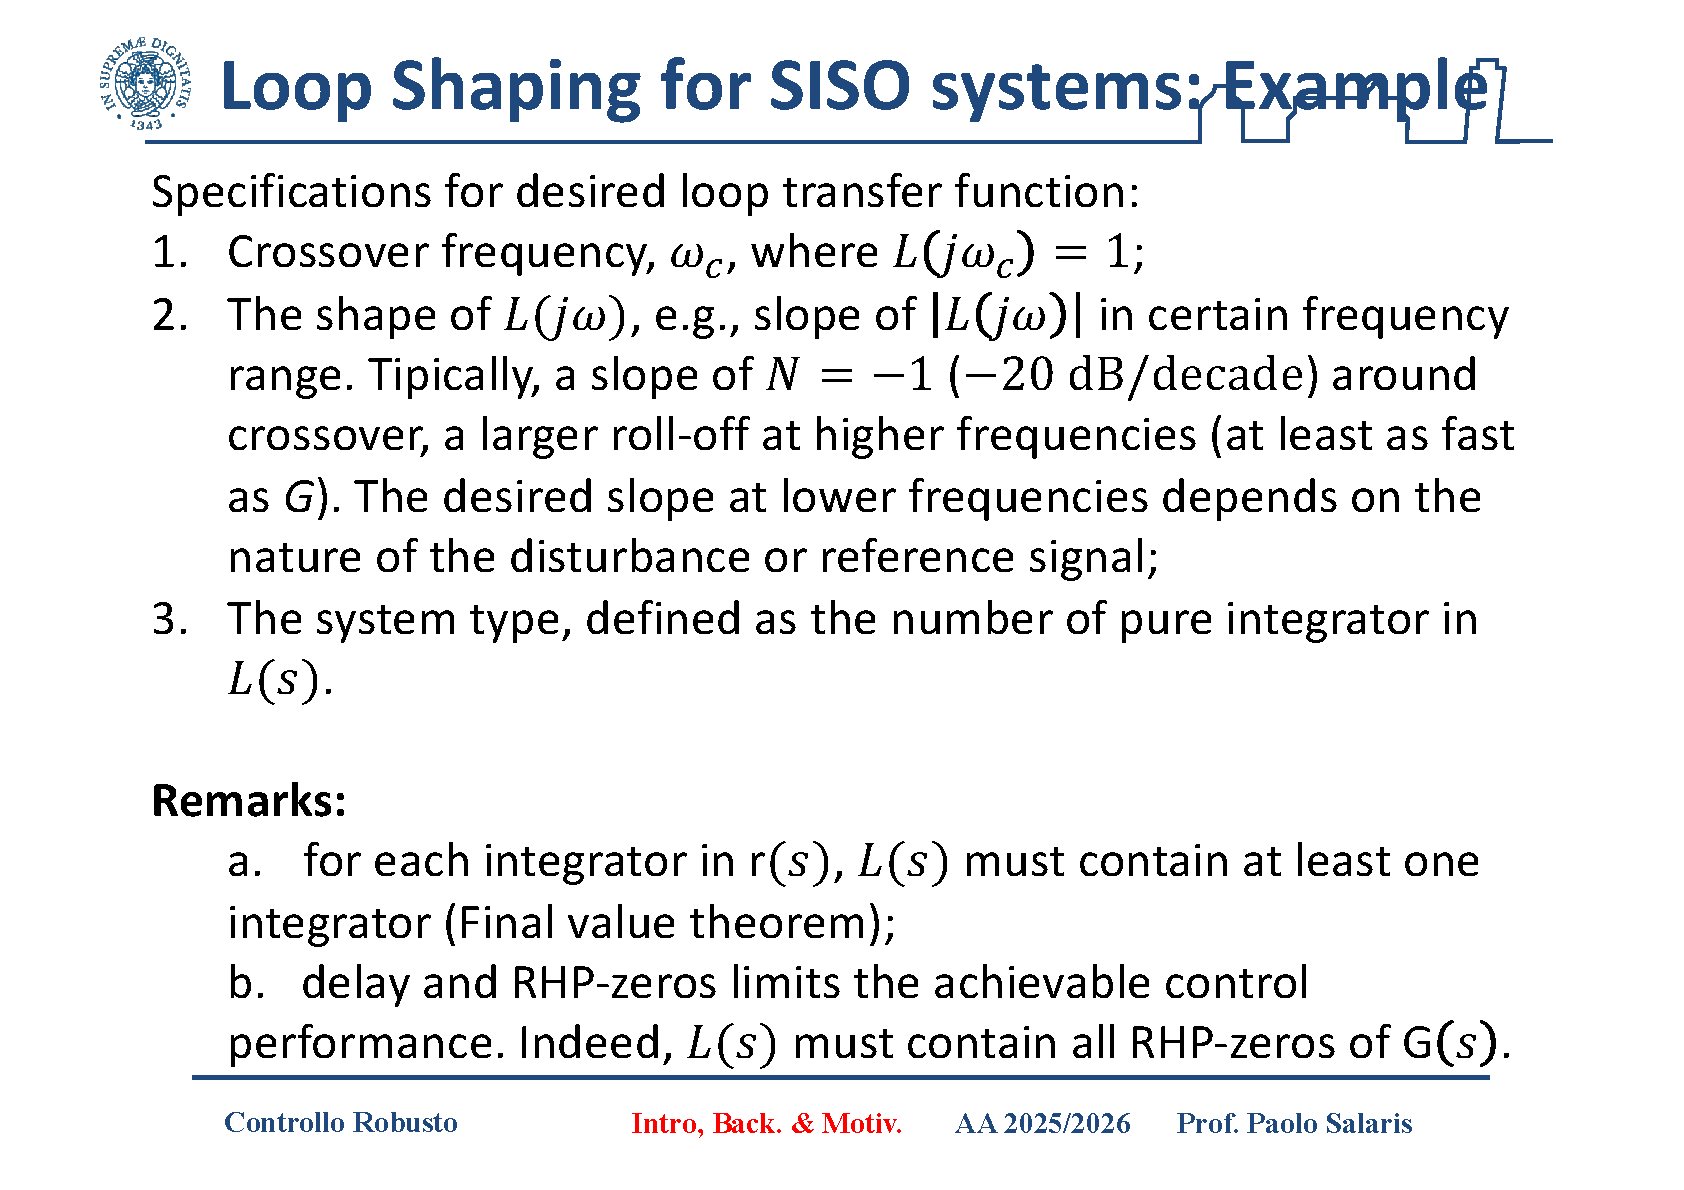
\includegraphics[width=\linewidth]{images5/intro-12x-003.png}
        \caption{Specifiche qualitative per la forma desiderata di $L(s)$: crossover, pendenza e tipo del sistema.}
    \end{subfigure}
    \hfill
    \begin{subfigure}{0.48\textwidth}
        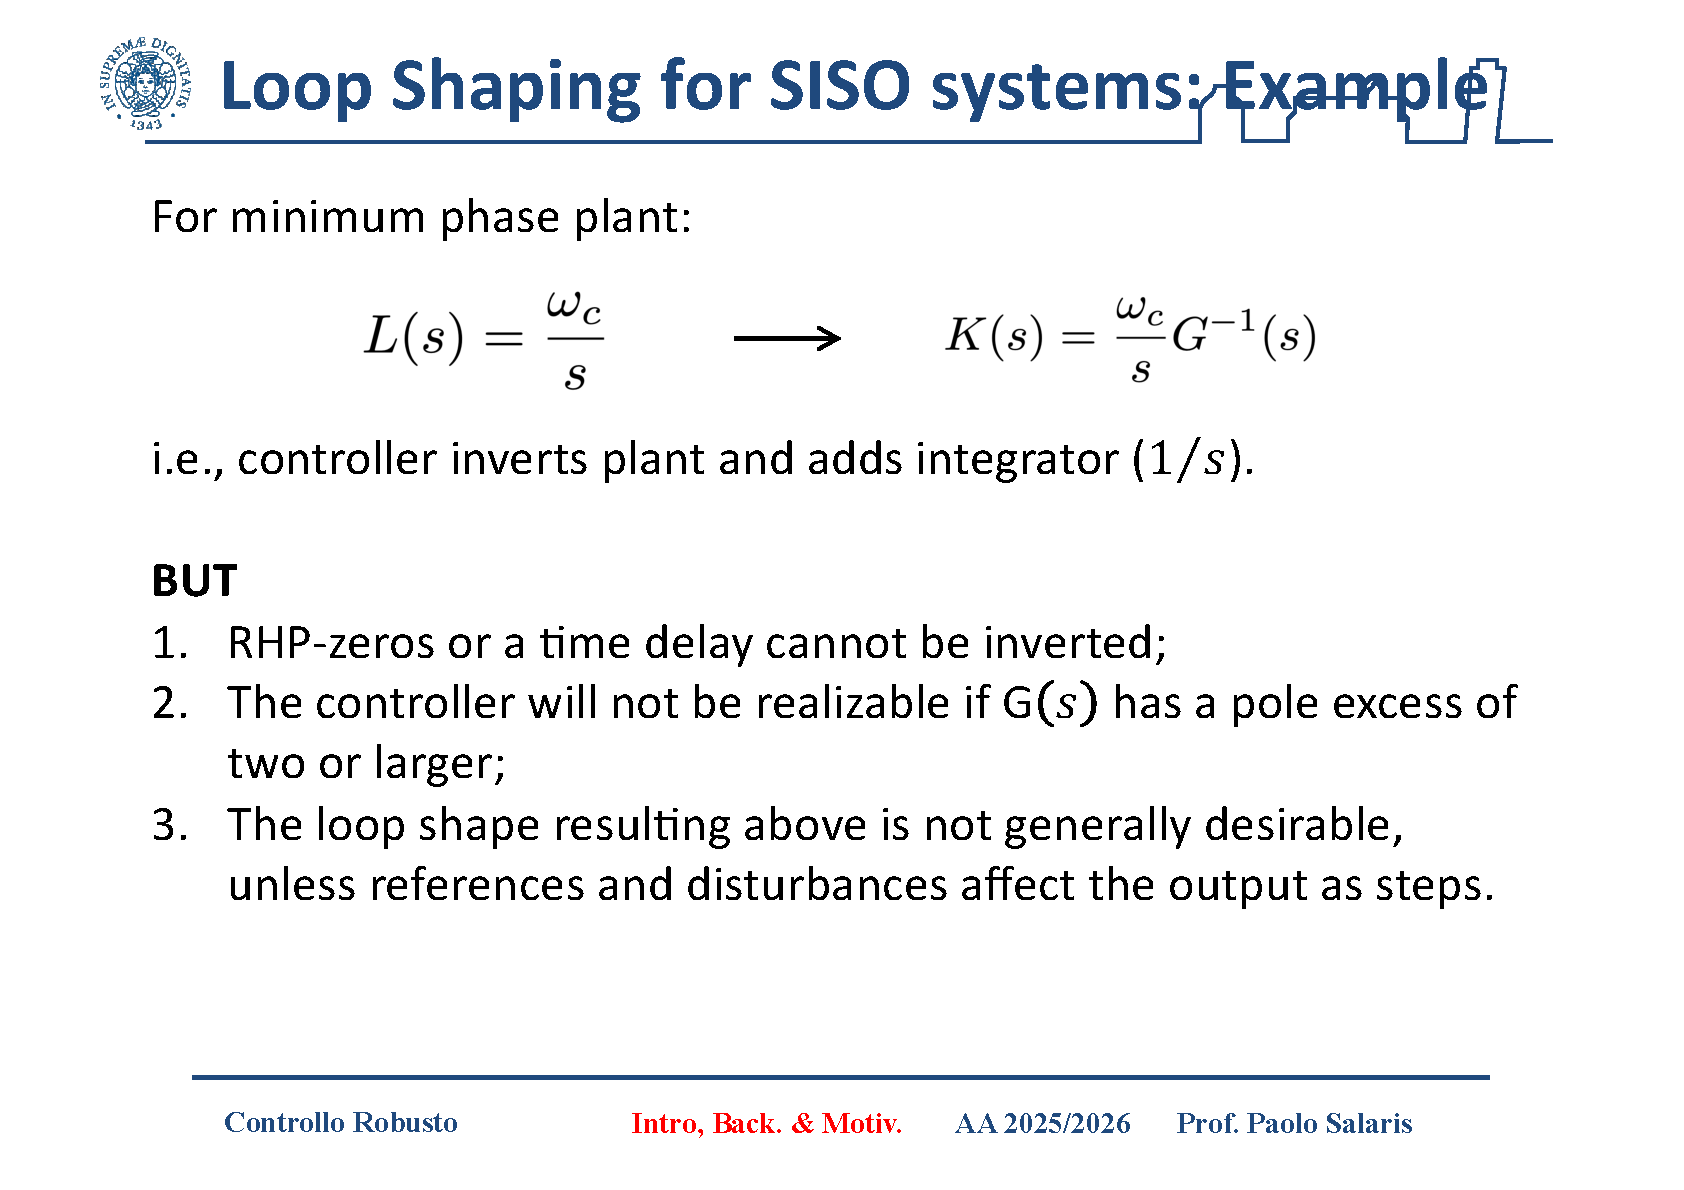
\includegraphics[width=\linewidth]{images5/intro-12x-004.png}
        \caption{Esempio ideale nel caso minimum phase e motivi per cui non può essere assunto come regola universale.}
    \end{subfigure}
    \caption{Le slide mostrano che il \emph{loop shaping} non consiste nel scegliere un controllore qualsiasi, ma nel dare a $L(s)$ una forma compatibile con prestazioni, realizzabilità e limiti strutturali del processo.}
\end{figure}

Questa chiusura del blocco precedente è importante anche pedagogicamente. Da un lato mostra \emph{che cosa} si vorrebbe rendere piccolo o grande progettando l'anello; dall'altro lascia aperta una domanda inevitabile: \emph{come misurare in modo rigoroso la grandezza di vettori, segnali e più avanti sistemi?} È esattamente la domanda a cui risponde il nuovo capitolo sulle norme.

\subsection{Ingresso al capitolo sulle norme}

La prima slide del nuovo PDF segna il cambio di registro. Dopo aver parlato di sensitività, loop shaping e margini, il corso introduce lo strumento matematico che permetterà di formulare molte di queste richieste in forma compatta e robusta: le norme. Anche se il titolo generale parla di ``signals and systems'', nelle prime dieci slide il lavoro si concentra soprattutto su vettori e segnali; le norme di sistema arriveranno naturalmente in seguito.

\begin{figure}[H]
    \centering
    
\includegraphics[width=0.78\textwidth]{images5/norms-01x-001.png}
    \caption{Slide di apertura del nuovo capitolo: il linguaggio delle norme viene introdotto come base matematica per il seguito del corso.}
\end{figure}

\subsection{Norme di vettori}

La definizione generale di norma su $\mathbb{R}^n$ richiede quattro proprietà:
\begin{align*}
\|x\| &\ge 0, \\
\|x\| &= 0 \iff x=0, \\
\|x+y\| &\le \|x\|+\|y\|, \\
\|\alpha x\| &= |\alpha|\,\|x\|.
\end{align*}
La prima dice che la norma non può essere negativa; la seconda che l'unico vettore di norma nulla è il vettore nullo; la terza è la disuguaglianza triangolare; la quarta è l'omogeneità assoluta. Insieme, queste proprietà formalizzano l'idea intuitiva di ``taglia'' o ``lunghezza'' di un vettore.

Le slide partono dalla norma euclidea
$$
\|x\|_2=\sqrt{x^T x}=\left(\sum_{i=1}^n |x_i|^2\right)^{1/2},
$$
e subito la collocano dentro la famiglia più generale delle norme $\ell_p$:
$$
\|x\|_p=\left(\sum_{i=1}^n |x_i|^p\right)^{1/p},
\qquad 1\le p < \infty,
$$
con il caso limite
$$
\|x\|_\infty=\max_i |x_i|=\lim_{p\to\infty}\|x\|_p.
$$

Questo punto merita un piccolo approfondimento. La norma $\ell_2$ misura la taglia complessiva del vettore in modo ``energetico'', perché somma i quadrati delle componenti. La norma $\ell_\infty$ guarda invece solo alla componente dominante, cioè al caso peggiore. La norma $\ell_1$ ha ancora un altro significato: misura la somma delle ampiezze assolute. In dimensione finita tutte queste norme sono equivalenti nel senso topologico, ma non sono equivalenti nel significato pratico: cambiano il modo in cui si valuta che cosa sia una componente grande, un errore distribuito o un errore concentrato su pochi canali.

\begin{figure}[H]
    \centering
    \begin{subfigure}{0.48\textwidth}
        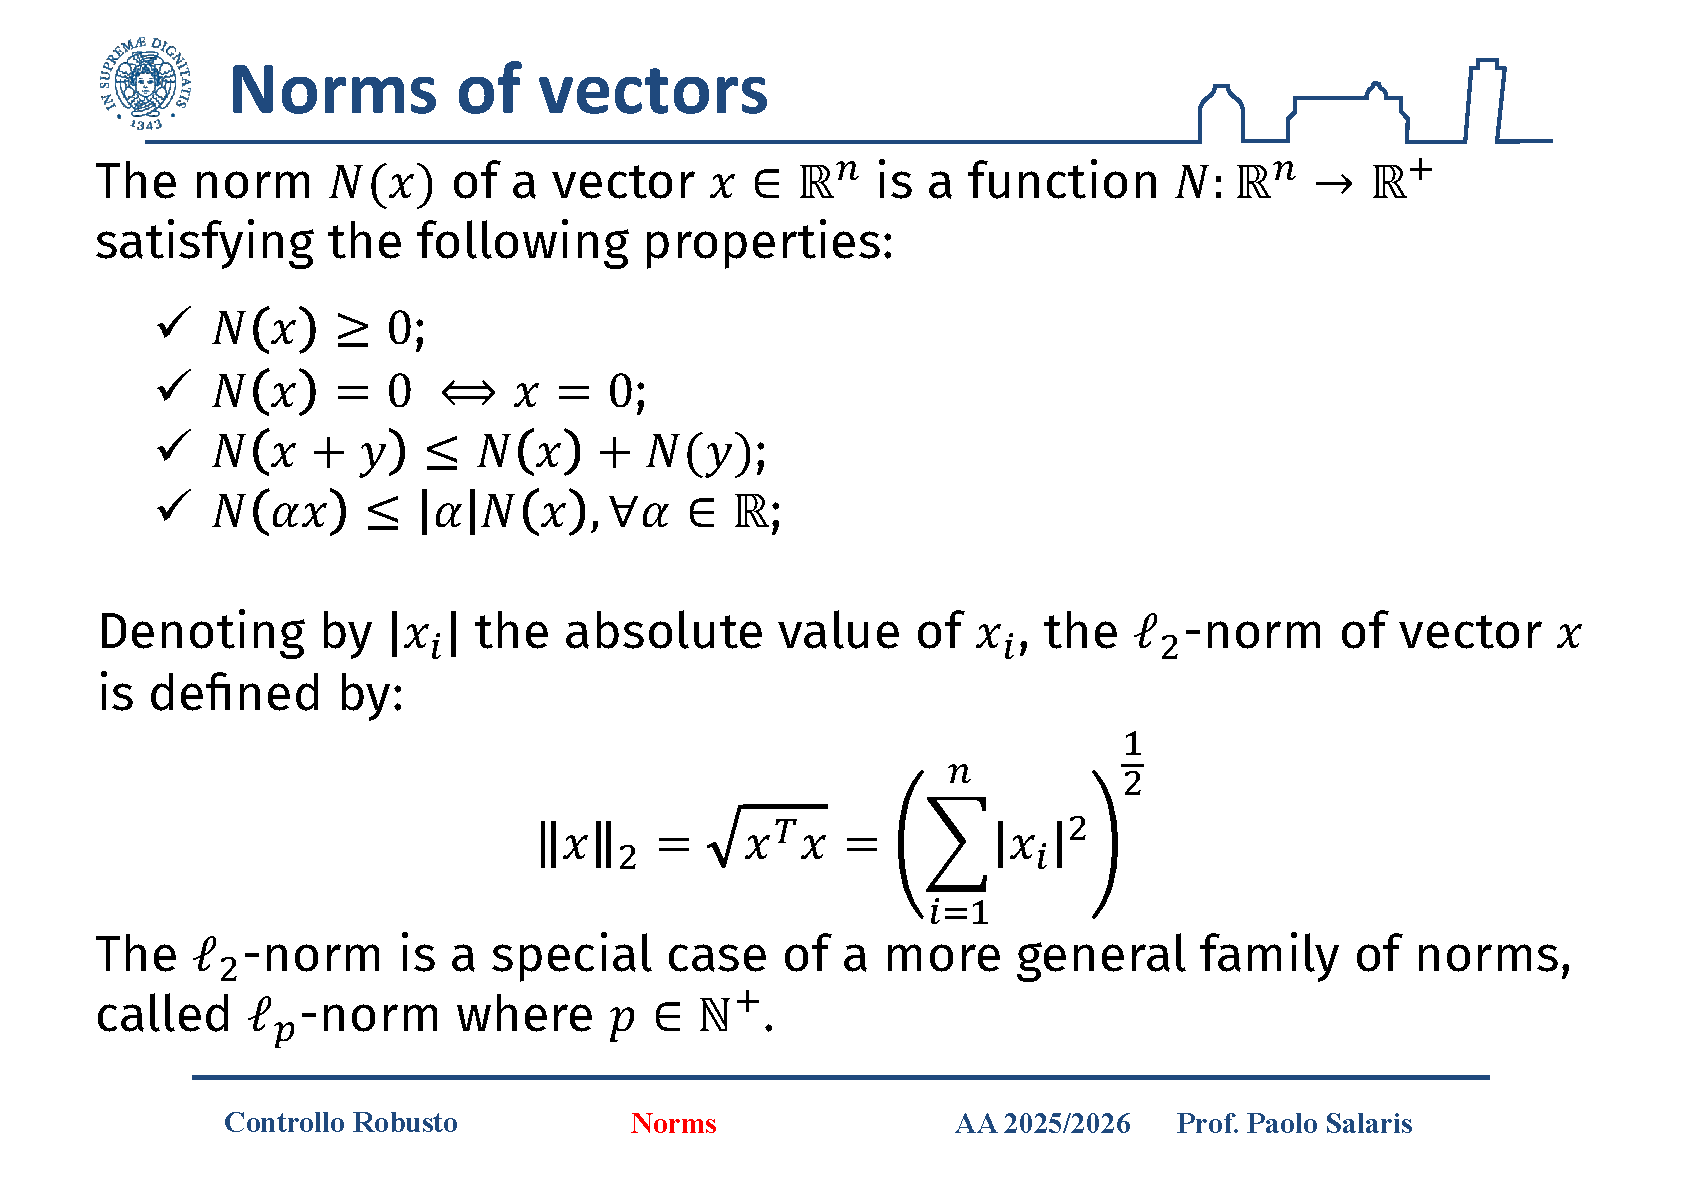
\includegraphics[width=\linewidth]{images5/norms-01x-002.png}
        \caption{Definizione assiomatica di norma e introduzione della norma euclidea.}
    \end{subfigure}
    \hfill
    \begin{subfigure}{0.48\textwidth}
        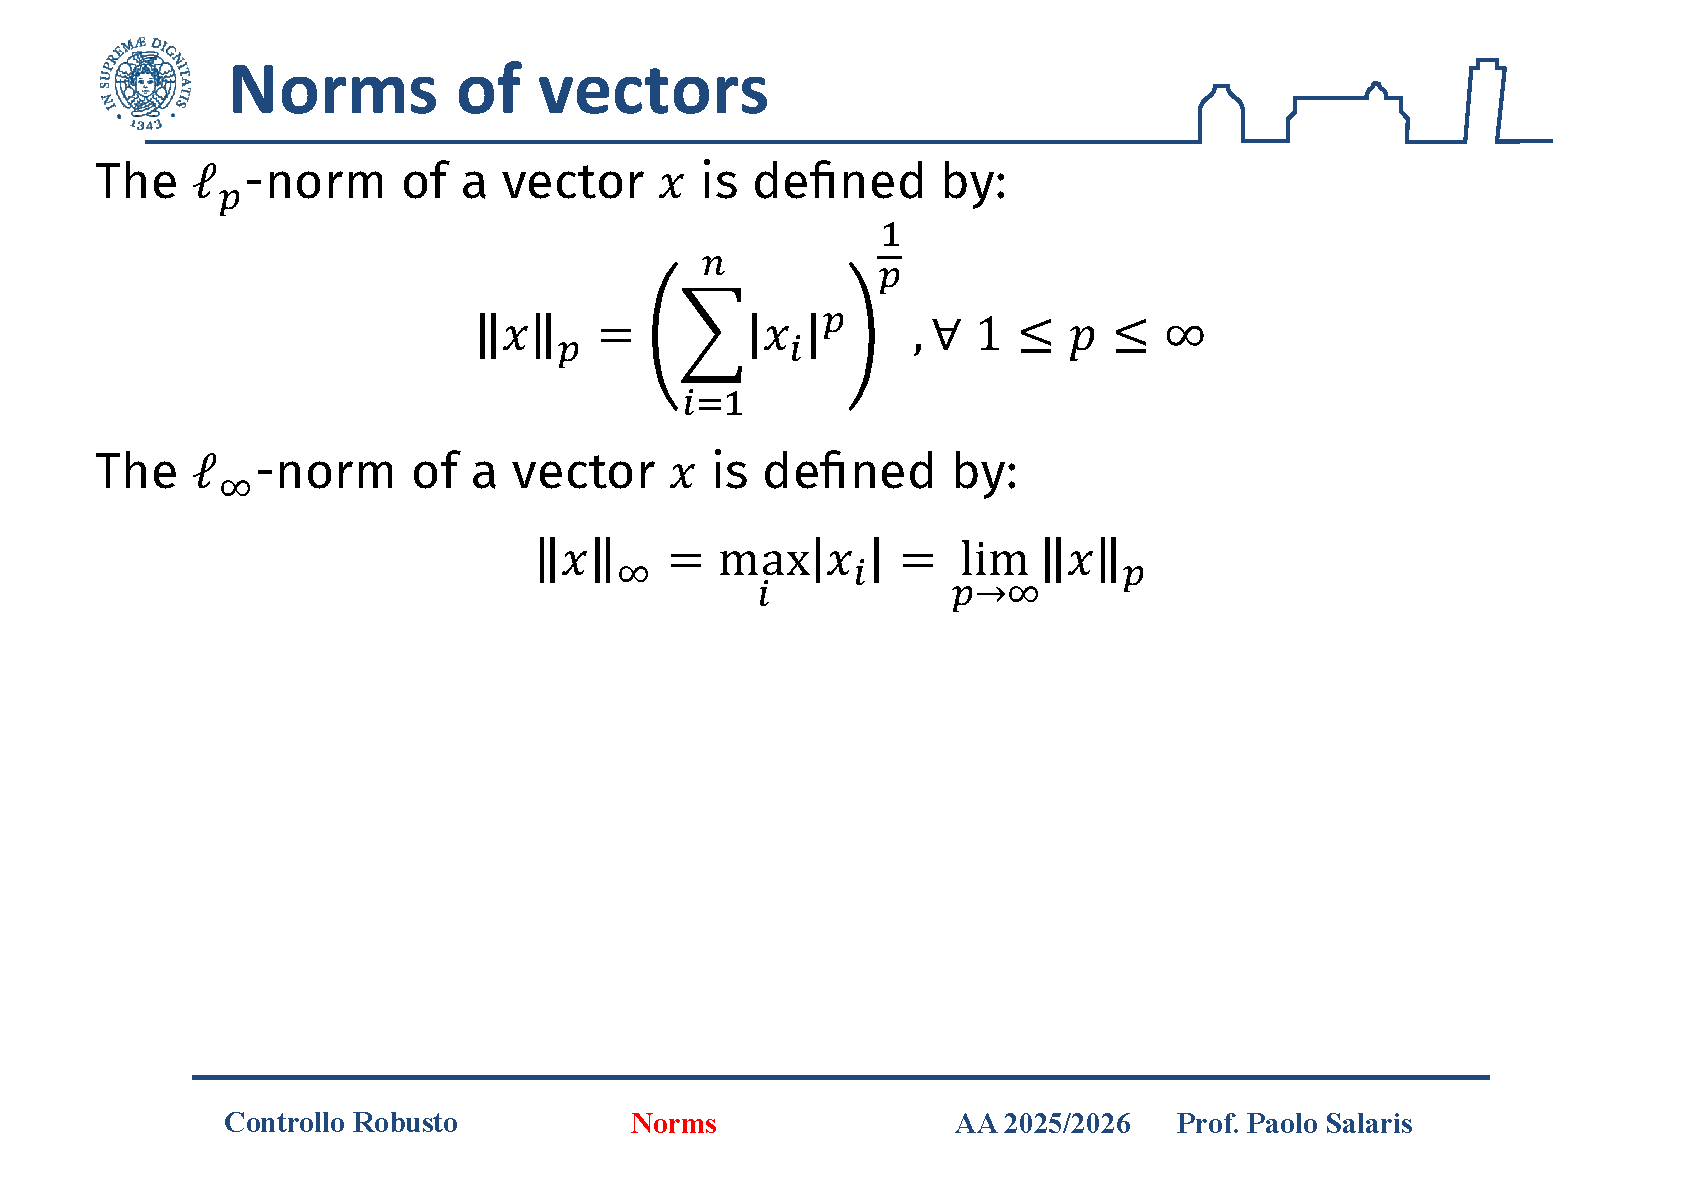
\includegraphics[width=\linewidth]{images5/norms-01x-003.png}
        \caption{Famiglia delle norme $\ell_p$ e caso limite $\ell_\infty$.}
    \end{subfigure}
    \caption{Le norme vettoriali introducono già la distinzione fondamentale tra misura energetica complessiva e misura di picco.}
\end{figure}

\begin{focusbox}
\textbf{Osservazione importante.} Su uno spazio vettoriale finito-dimensionale cambiare norma non cambia la nozione di convergenza o continuità, ma cambia le costanti e soprattutto il significato operativo della misura. Quando si passerà ai segnali e ai sistemi, questa scelta diventerà ancora più sostanziale.
\end{focusbox}

\subsection{Norme di segnali}

\subsubsection{Norma \texorpdfstring{$L_2$}{L2} di un segnale scalare}

Per un segnale scalare $v(t)$ definito su $t\ge 0$, la norma $L_2$ viene definita come
$$
\|v\|_2=\sqrt{\int_0^\infty v^2(\tau)\,d\tau}.
$$
Nel caso reale questa quantità misura direttamente l'energia del segnale; nel caso complesso si userebbe il modulo quadro. È qui che il passaggio dai vettori ai segnali mostra la sua natura: una somma finita viene sostituita da un integrale, cioè da un accumulo continuo nel tempo.

La slide sottolinea proprio questa lettura fisica. Se $v(t)$ è una tensione o una corrente, allora $\|v\|_2^2$ è proporzionale all'energia associata al segnale. Per il controllo questa interpretazione è preziosa, perché molte richieste pratiche hanno davvero la forma ``mantenere piccola l'energia del disturbo trasmesso'' oppure ``limitare l'energia del comando''.

Il passo successivo è il teorema di Parseval, che permette di riscrivere la stessa quantità nel dominio della frequenza:
$$
\|V\|_2=\sqrt{\frac{1}{2\pi}\int_{-\infty}^{\infty}|V(j\omega)|^2\,d\omega}.
$$
Questa identità è molto più di un cambio di variabile. Dice che la stessa energia può essere misurata nel tempo o nella frequenza senza perdita di informazione. Il fattore $1/(2\pi)$ dipende dalla convenzione adottata per la trasformata di Fourier/Laplace.

\begin{figure}[H]
    \centering
    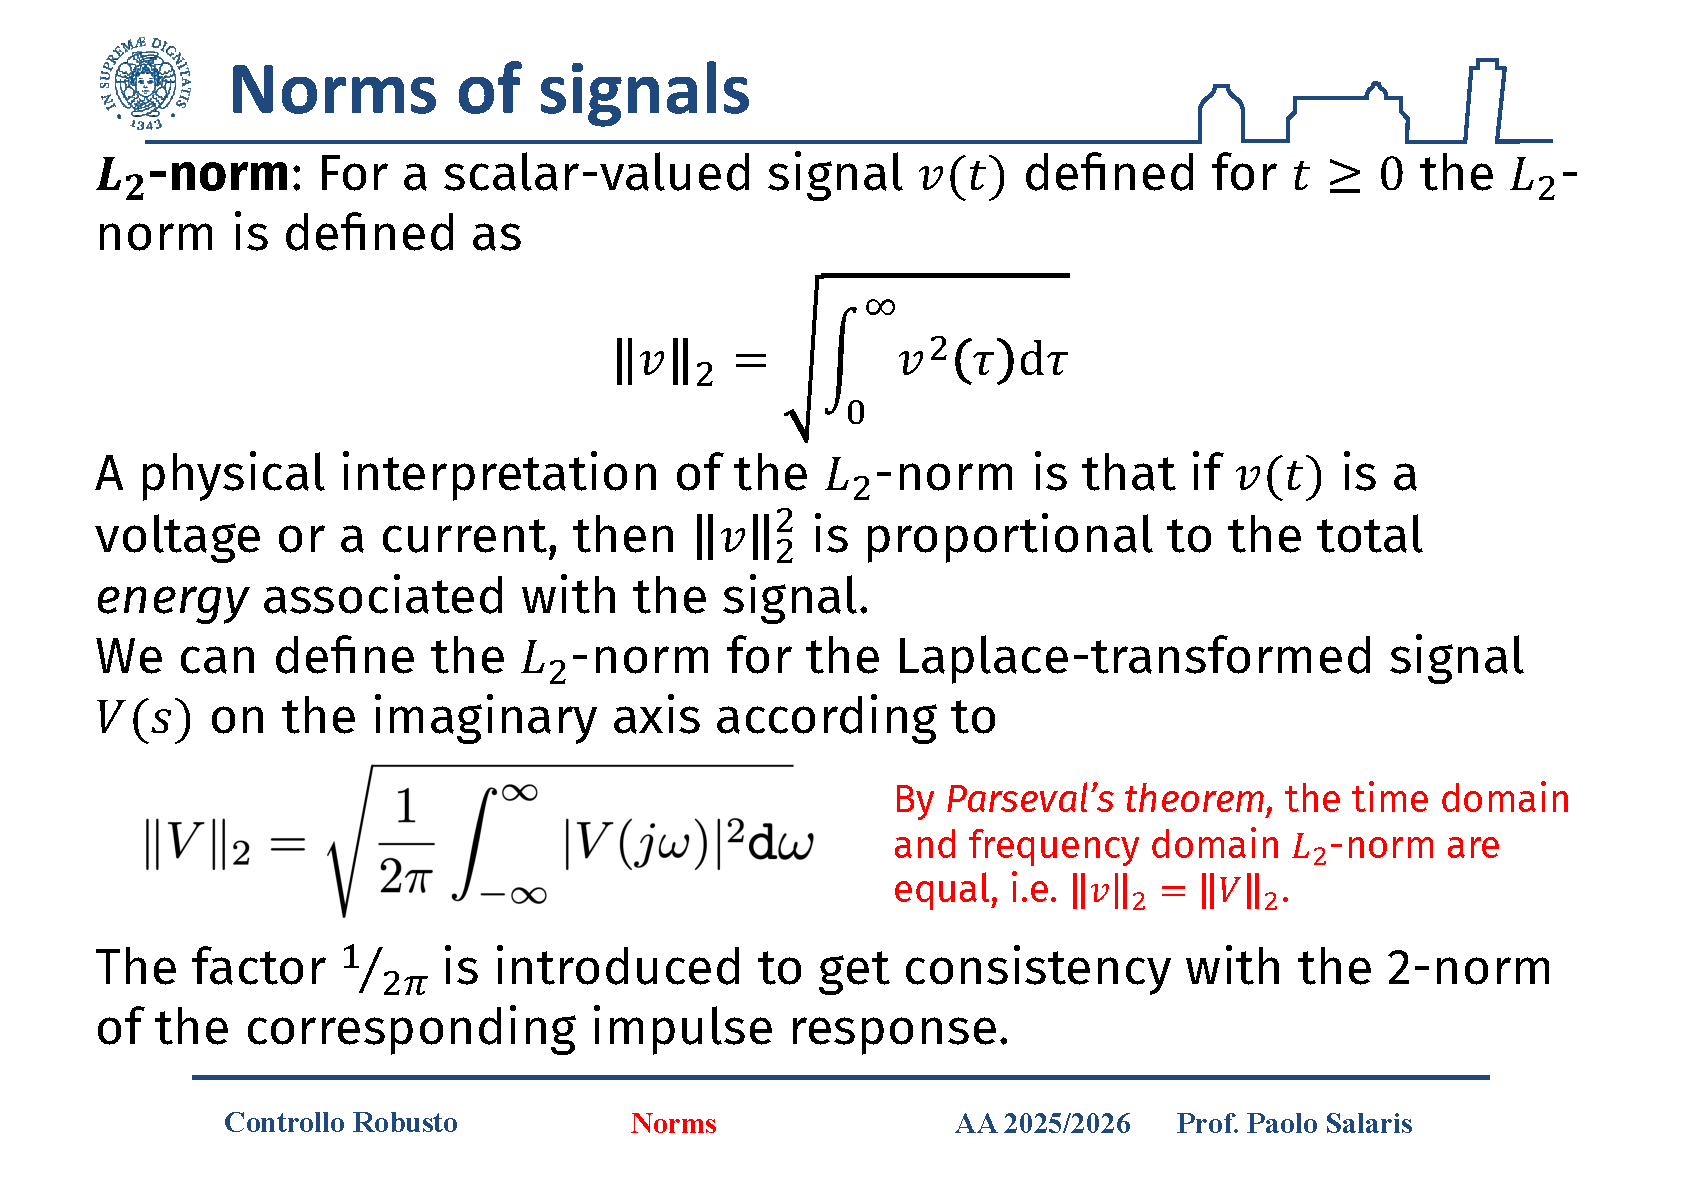
\includegraphics[width=0.82\textwidth]{images5/norms-01x-004.png}
    \caption{La norma $L_2$ di un segnale scalare è letta come energia nel tempo e, tramite Parseval, come area spettrale nel dominio della frequenza.}
\end{figure}

\subsubsection{Segnali vettoriali e forma spettrale della norma}

Per un segnale vettoriale
$$
v(t)=\begin{bmatrix}v_1(t) & \cdots & v_m(t)\end{bmatrix}^T,
$$
la generalizzazione naturale è
$$
\|v\|_2
=
\sqrt{\int_0^\infty v^T(\tau)v(\tau)\,d\tau}
=
\sqrt{\int_0^\infty \sum_{i=1}^m v_i^2(\tau)\,d\tau}.
$$
Questa formula conferma l'interpretazione energetica: l'energia totale del segnale vettoriale è la somma delle energie dei singoli canali.

Nel dominio di Laplace/frequenza la stessa idea si traduce nella quantità
$$
\|V\|_2
=
\sqrt{\frac{1}{2\pi}\int_{-\infty}^{\infty}V^T(-j\omega)V(j\omega)\,d\omega}
=
\sqrt{\frac{1}{2\pi}\int_{-\infty}^{\infty}\sum_{i=1}^m |V_i(j\omega)|^2\,d\omega}.
$$
La scrittura con $V^T(-j\omega)V(j\omega)$ è particolarmente comoda perché prepara il collegamento con il calcolo complesso: al posto di sommare esplicitamente i contributi dei vari canali, si raccoglie tutto in un unico prodotto scalare frequenziale.

\begin{figure}[H]
    \centering
    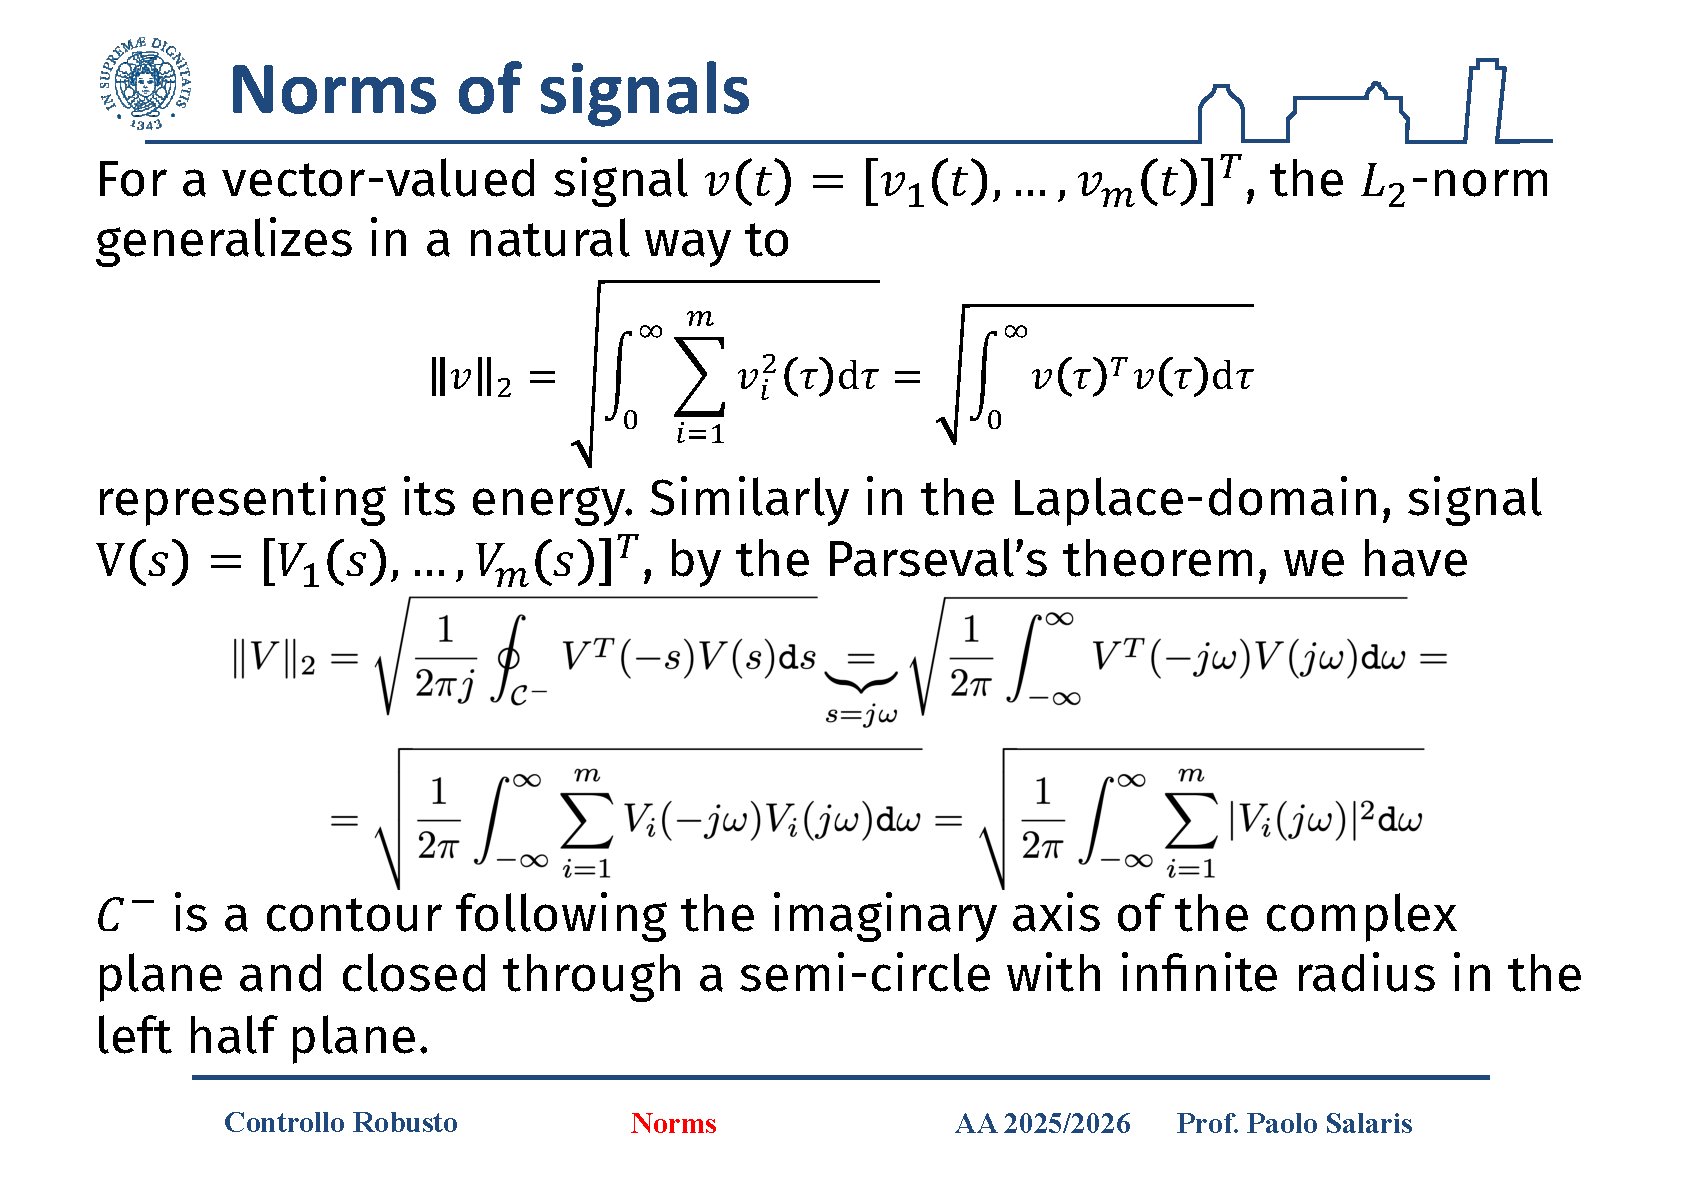
\includegraphics[width=0.84\textwidth]{images5/norms-01x-005.png}
    \caption{La norma $L_2$ di un segnale vettoriale mantiene la lettura energetica e si presta a una formulazione compatta nel dominio di Laplace.}
\end{figure}

\subsubsection{Teorema dei residui e calcolo della norma}

La slide successiva introduce lo strumento tecnico che rende questi calcoli particolarmente eleganti: il teorema dei residui. Se si considera il contorno $C^-$ che segue l'asse immaginario e si chiude nel semipiano sinistro, allora per segnali stabili si può trasformare l'integrale spettrale in una somma di residui delle singolarità interne al contorno. In forma sintetica:
$$
\oint_{C^-} f(s)\,ds
=
2\pi j\sum_k \operatorname{Res}(f,\lambda_k).
$$

Applicato alla funzione
$$
f(s)=V^T(-s)V(s),
$$
questo porta a una formula molto utile:
$$
\|V\|_2
=
\sqrt{\sum_{\lambda_k \in \mathbb{C}_-} \operatorname{Res}\!\bigl(V^T(-s)V(s),\lambda_k\bigr)}.
$$
Il significato pratico è notevole: invece di integrare su tutte le frequenze, si può spesso lavorare direttamente con i poli di $V(s)$ nel semipiano sinistro. Per poli semplici, il residuo si calcola con la formula elementare
$$
\operatorname{Res}(F,\lambda)=\lim_{s\to \lambda}(s-\lambda)F(s),
$$
mentre per poli multipli si usa la formula con la derivata riportata in slide.

\begin{figure}[H]
    \centering
    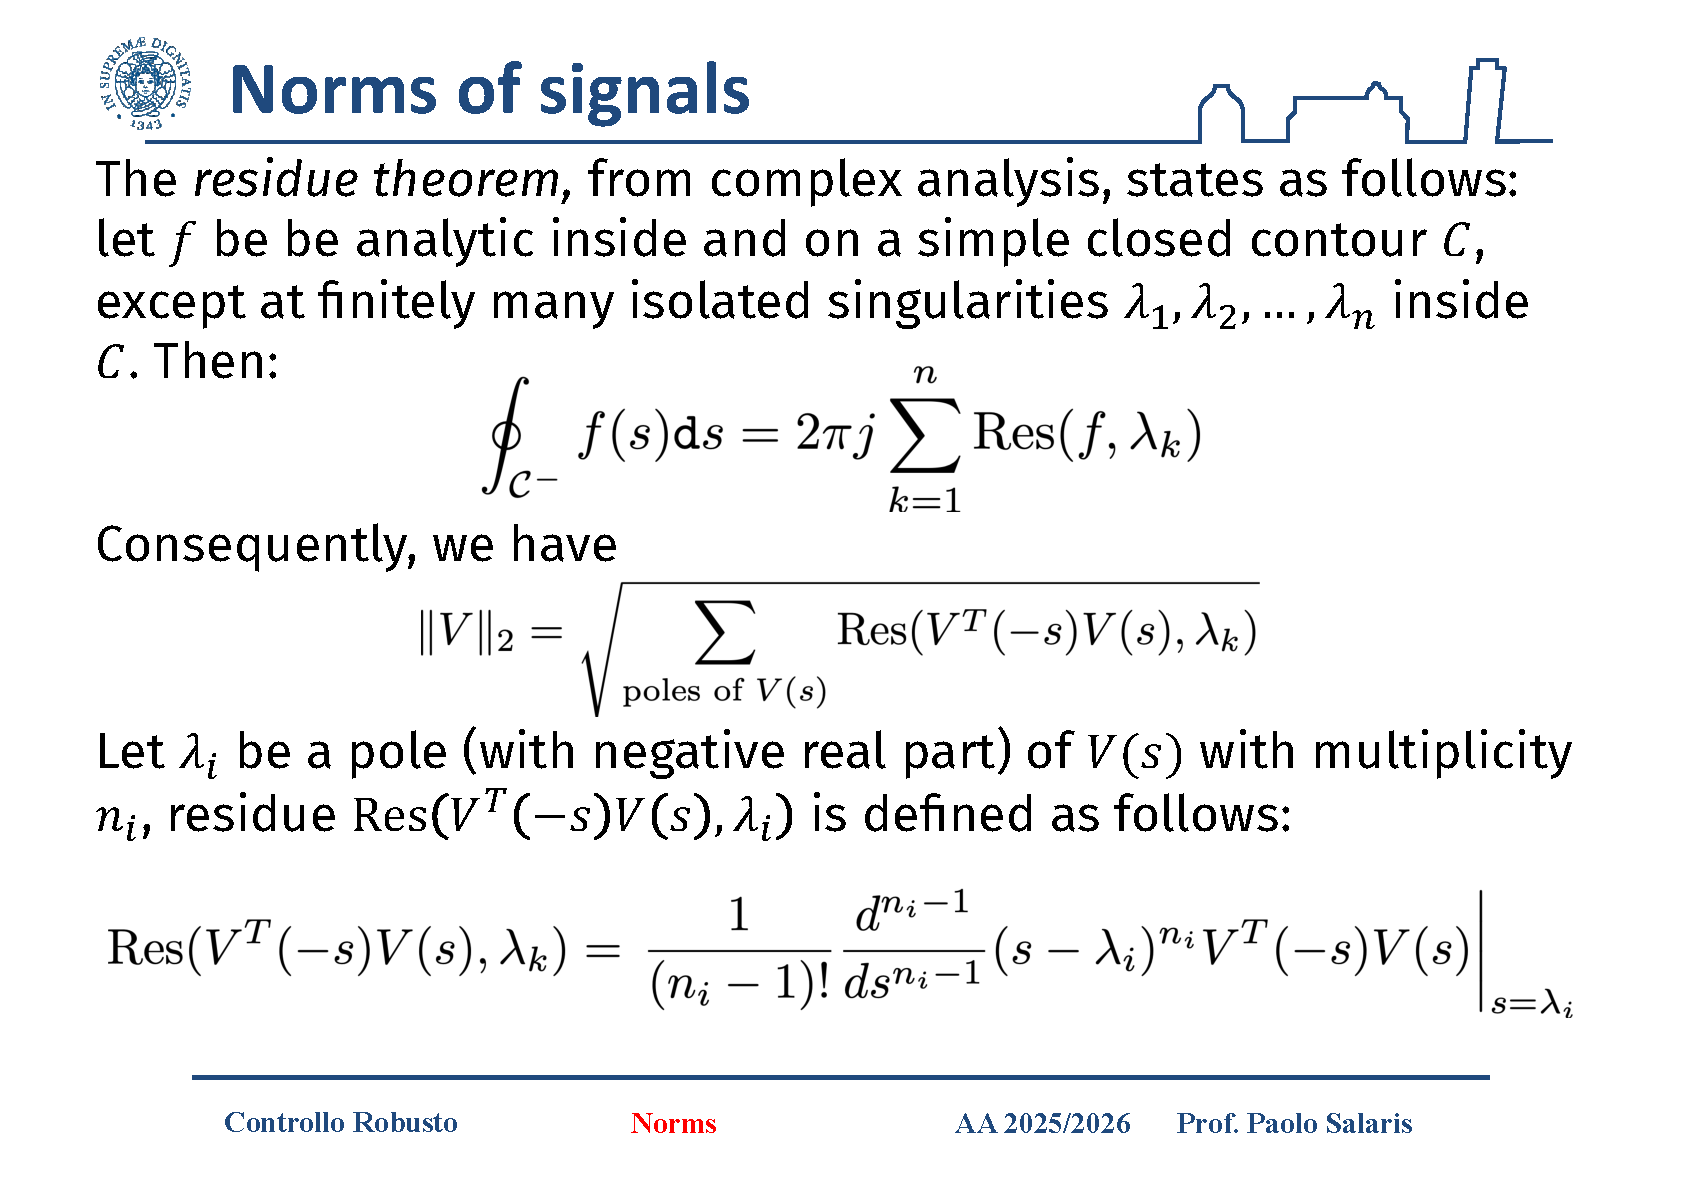
\includegraphics[width=0.84\textwidth]{images5/norms-01x-006.png}
    \caption{Il teorema dei residui trasforma il calcolo della norma $L_2$ in un problema locale sui poli della trasformata del segnale.}
\end{figure}

\subsection{Esempi di calcolo della norma \texorpdfstring{$L_2$}{L2}}

\subsubsection{Esempio 1: segnale scalare esponenziale}

Nel primo esempio il segnale è
$$
x(t)=e^{-t/T},
\qquad T>0,
$$
e la sua norma si calcola direttamente nel tempo come
$$
\|x\|_2
=
\sqrt{\int_0^\infty e^{-2t/T}\,dt}
=
\sqrt{\frac{T}{2}}.
$$
La slide mostra poi il percorso equivalente nel dominio di Laplace. La trasformata è
$$
X(s)=\frac{1}{s+1/T}=\frac{T}{Ts+1},
$$
da cui
$$
X^T(-s)X(s)=\frac{T^2}{(1+Ts)(1-Ts)}.
$$
Poiché l'unico polo nel semipiano sinistro è $\lambda_1=-1/T$, il residuo corrispondente vale
$$
\operatorname{Res}\!\bigl(X^T(-s)X(s),\lambda_1\bigr)=\frac{T}{2},
$$
e quindi di nuovo
$$
\|x\|_2=\sqrt{\frac{T}{2}}.
$$
L'esempio è semplice, ma fa vedere molto bene il metodo: la norma $L_2$ si può leggere come integrale temporale, come integrale spettrale o come somma di contributi locali associati ai poli.

\begin{figure}[H]
    \centering
    \begin{subfigure}{0.48\textwidth}
        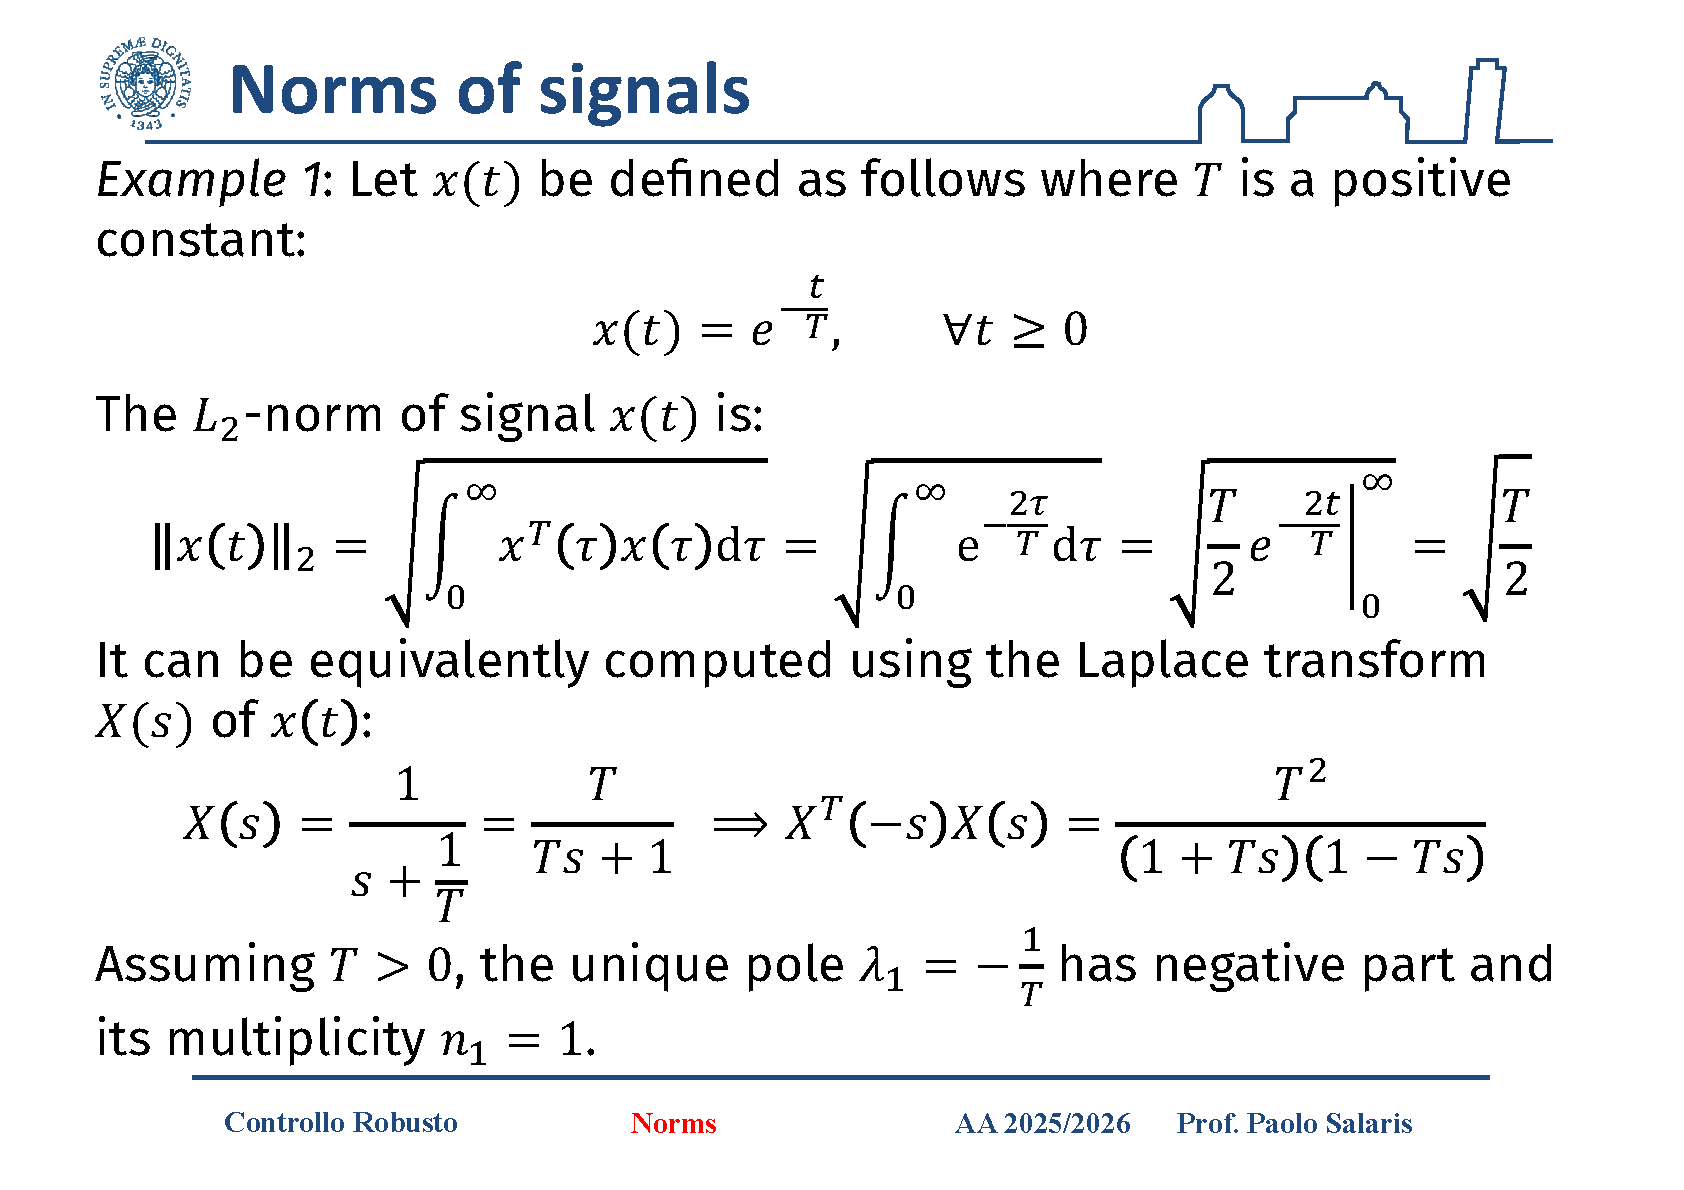
\includegraphics[width=\linewidth]{images5/norms-01x-007.png}
        \caption{Calcolo diretto nel dominio del tempo e preparazione del calcolo in Laplace.}
    \end{subfigure}
    \hfill
    \begin{subfigure}{0.48\textwidth}
        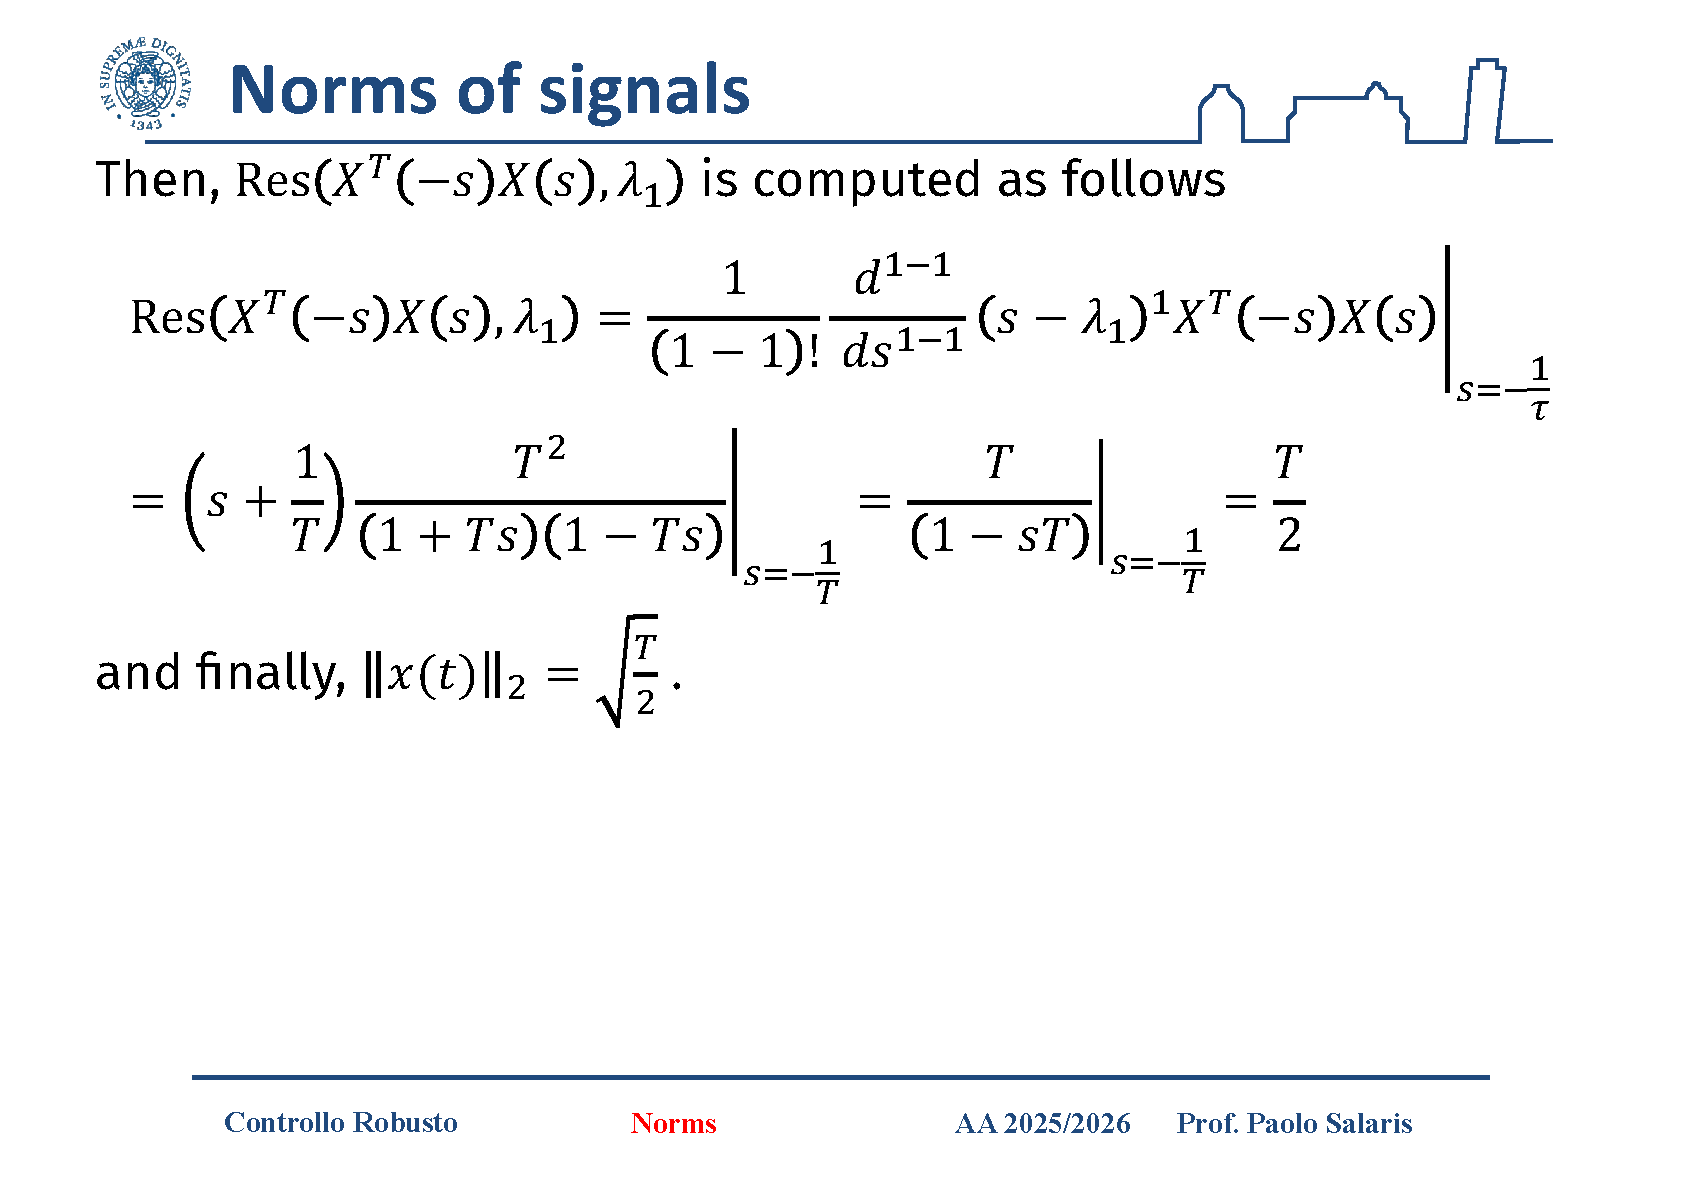
\includegraphics[width=\linewidth]{images5/norms-01x-008.png}
        \caption{Calcolo del residuo e ottenimento della stessa norma tramite la trasformata del segnale.}
    \end{subfigure}
    \caption{Il primo esempio mostra la perfetta coerenza tra interpretazione energetica nel tempo e calcolo complesso nel dominio di Laplace.}
\end{figure}

\subsubsection{Esempio 2: segnale vettoriale}

Nel secondo esempio si considera il segnale vettoriale
$$
x(t)=
\begin{bmatrix}
e^{-t}\\
e^{-2t}
\end{bmatrix},
\qquad t\ge 0.
$$
Nel dominio del tempo la norma si ottiene sommando le energie dei due canali:
$$
\|x\|_2
=
\sqrt{\int_0^\infty \bigl(e^{-2t}+e^{-4t}\bigr)\,dt}
=
\sqrt{\frac{1}{2}+\frac{1}{4}}
=
\sqrt{\frac{3}{4}}.
$$

Nel dominio di Laplace, invece,
$$
X(s)=
\begin{bmatrix}
\dfrac{1}{s+1}\\[0.4em]
\dfrac{1}{s+2}
\end{bmatrix},
$$
e dunque
$$
X^T(-s)X(s)
=
\frac{1}{(-s+1)(s+1)}
\;+\;
\frac{1}{(-s+2)(s+2)}.
$$
I poli nel semipiano sinistro sono $\lambda_1=-1$ e $\lambda_2=-2$, entrambi semplici. I residui valgono rispettivamente
$$
\operatorname{Res}\!\bigl(X^T(-s)X(s),-1\bigr)=\frac{1}{2},
\qquad
\operatorname{Res}\!\bigl(X^T(-s)X(s),-2\bigr)=\frac{1}{4},
$$
per cui
$$
\|x\|_2
=
\sqrt{\frac{1}{2}+\frac{1}{4}}
=
\sqrt{\frac{3}{4}}.
$$

Questo esempio aggiunge un'informazione importante rispetto al precedente: nel caso vettoriale la norma totale non è altro che la combinazione energetica dei singoli canali. Ciò anticipa già il modo in cui, più avanti, si leggeranno prestazioni multi-canale e norme di sistemi MIMO.

\begin{figure}[H]
    \centering
    \begin{subfigure}{0.48\textwidth}
        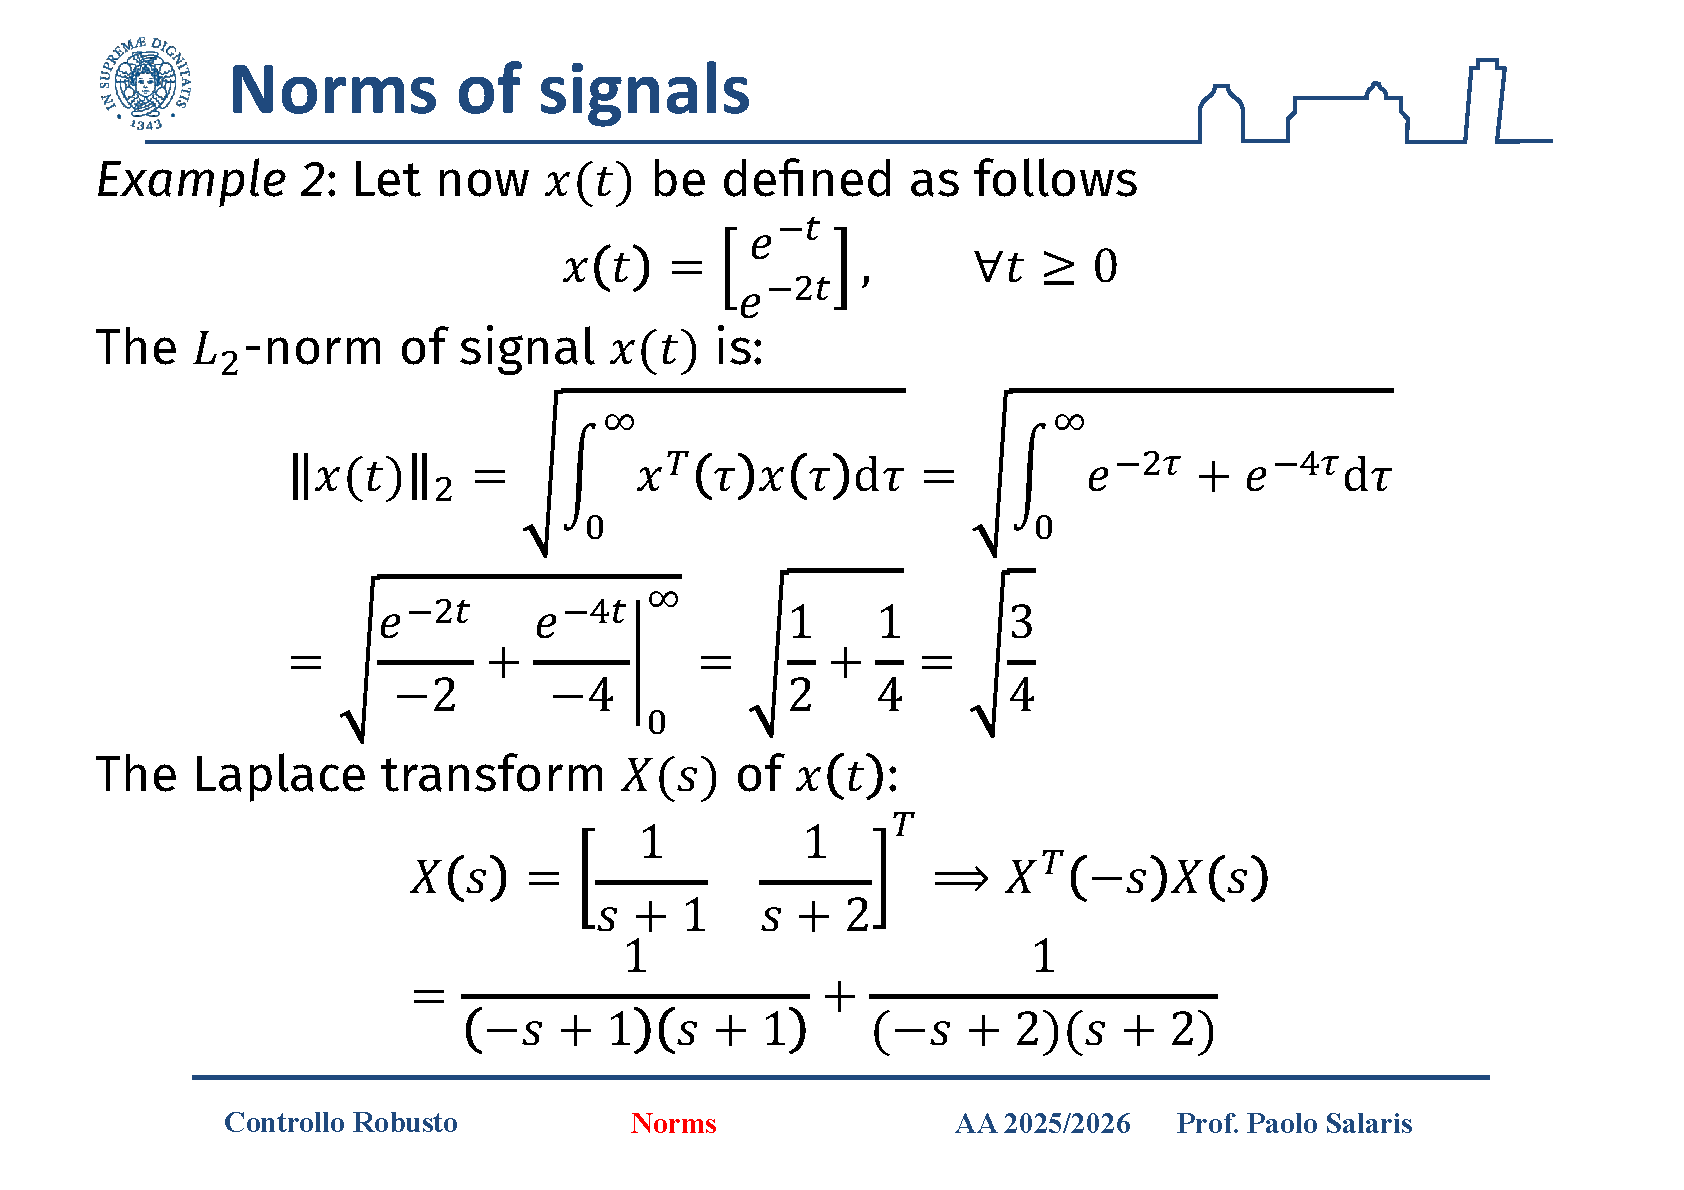
\includegraphics[width=\linewidth]{images5/norms-01x-009.png}
        \caption{Calcolo diretto della norma del segnale vettoriale e costruzione di $X^T(-s)X(s)$.}
    \end{subfigure}
    \hfill
    \begin{subfigure}{0.48\textwidth}
        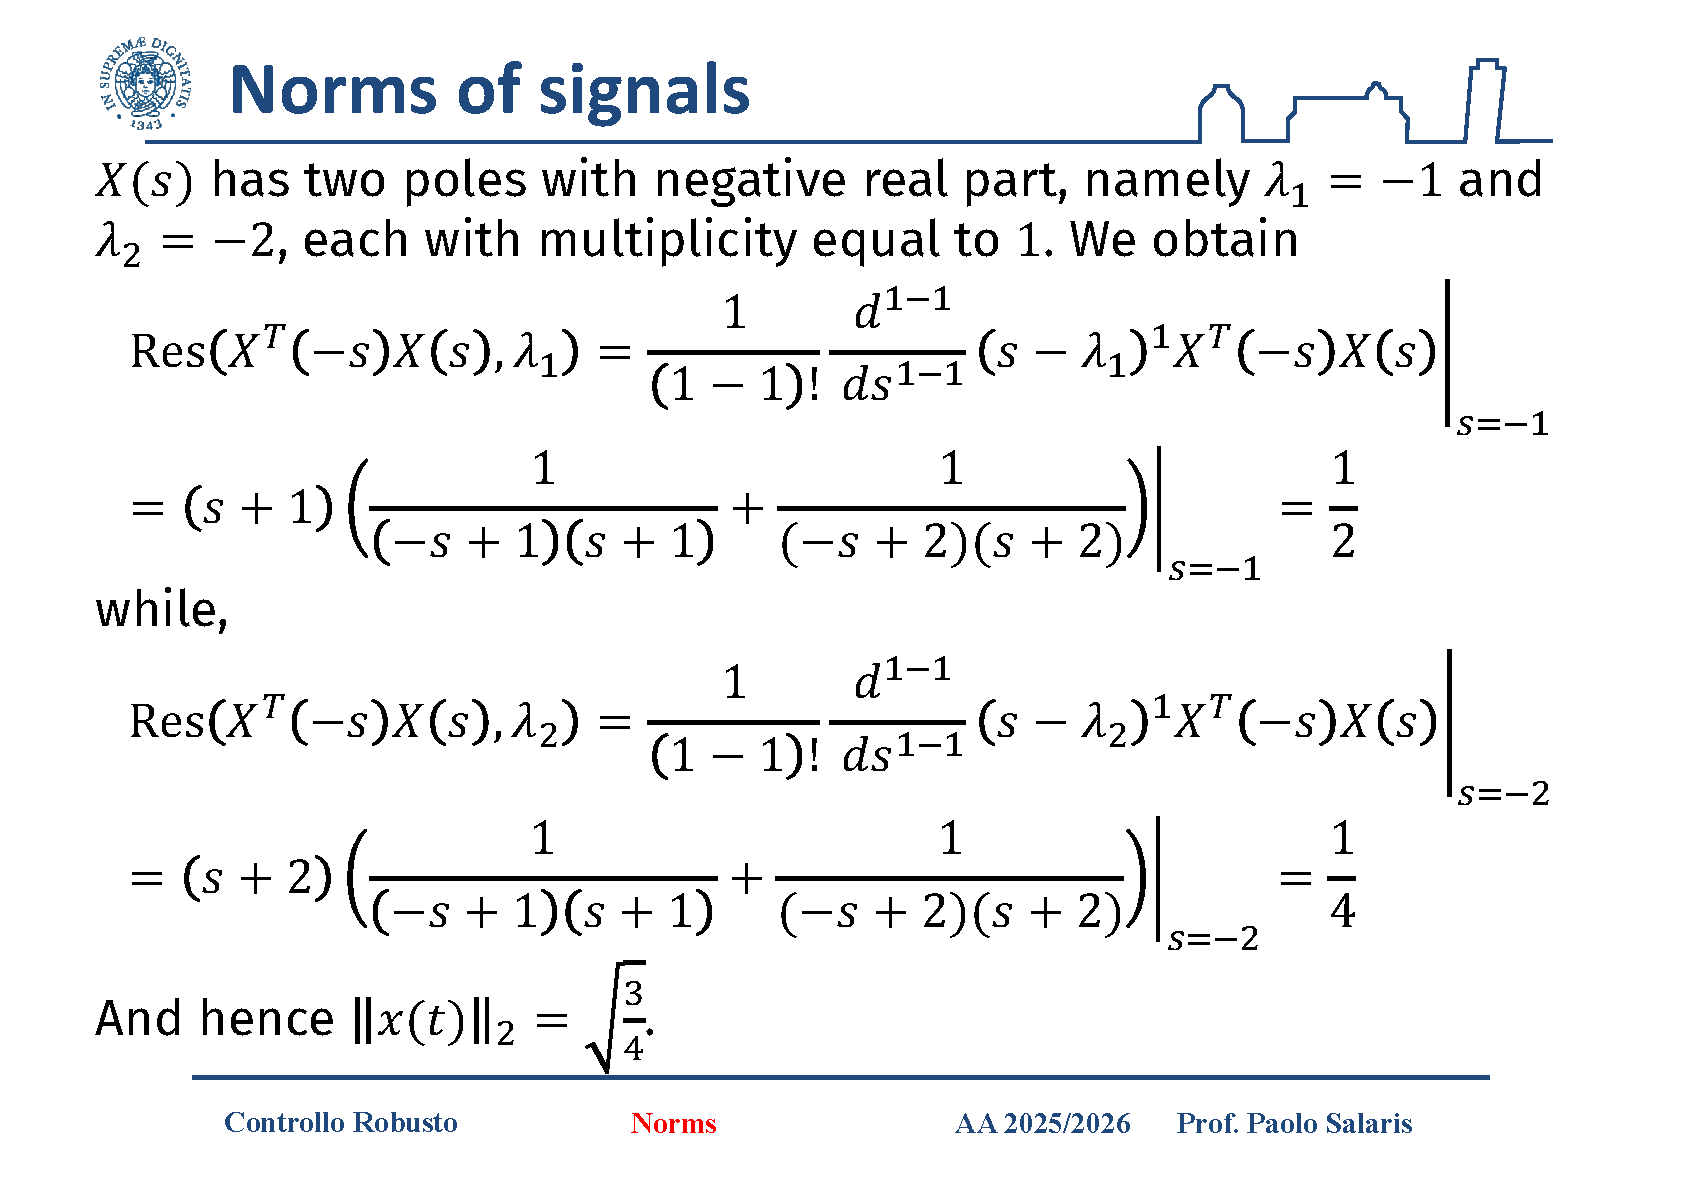
\includegraphics[width=\linewidth]{images5/norms-01x-010.png}
        \caption{Somma dei residui dei poli nel semipiano sinistro e recupero della stessa norma.}
    \end{subfigure}
    \caption{Il secondo esempio mostra che il passaggio ai segnali vettoriali non cambia il metodo, ma solo il numero di contributi da sommare.}
\end{figure}

\subsection{Sintesi conclusiva della lezione}

La Lezione 6 svolge dunque due funzioni complementari. La prima è chiudere con chiarezza il discorso sul \emph{loop shaping} SISO, mostrando che indici come $M_s$ e $M_t$ sono già vere norme dei canali chiusi e quindi veri strumenti quantitativi di progetto. La seconda è introdurre il linguaggio generale delle norme di vettori e segnali, che permetterà di estendere questo modo di pensare a oggetti sempre più ricchi.

Sul piano concettuale, il passaggio decisivo è questo: una specifica di controllo robusto non dice soltanto che un certo errore deve essere ``piccolo''; deve dire \emph{quanto piccolo}, \emph{in quale senso} e \emph{rispetto a quale aggregazione} delle sue componenti o frequenze. Le norme servono precisamente a rispondere a queste tre domande.

Sul piano operativo, la lezione lascia in mano tre strumenti concreti: la famiglia delle norme $\ell_p$ per vettori, la norma $L_2$ per segnali come misura di energia, e la possibilità di calcolare tale norma sia tramite Parseval sia tramite residui. È su questa base che il corso potrà poi introdurre con naturalezza le norme di sistema e le specifiche robuste in forma compatta.

\clearpage
\phantomsection
\section*{Appendice}
\addcontentsline{toc}{section}{Appendice}

\subsection*{Nota sulla notazione delle norme}
\phantomsection
\addcontentsline{toc}{subsection}{Nota sulla notazione delle norme}

Nel testo si segue la convenzione delle slide: $\ell_p$ indica le norme di vettori a dimensione finita, mentre $L_2$ indica la norma energetica di segnali continui nel tempo. Inoltre, nelle formule frequenziali compare spesso $V^T(-s)V(s)$, che va letto come prodotto naturale nel caso di segnali reali. Nel caso complesso la scrittura corretta diventa normalmente $V^*(-j\omega)V(j\omega)$, cioè con trasposto coniugato.

\subsection*{Riferimento al materiale originale}
\phantomsection
\addcontentsline{toc}{subsection}{Riferimento al materiale originale}

Questa parte del documento è una traduzione e rielaborazione estesa delle slide 121--124 del PDF ``Controllo Robusto Intro, Back.\ \& Motiv.'' e delle slide 1--10 del PDF ``Norms for signals and systems'', caricate dall'utente come materiale di partenza.

\begin{coverpage}
\centering
{\Huge\bfseries Controllo Robusto\par}
\vspace{0.4em}
{\LARGE Traduzione in italiano e approfondimento\par}
\vspace{0.5em}
{\Large Norme dei segnali e norma \texorpdfstring{$H_2$}{H2} dei sistemi\par}
\vfill
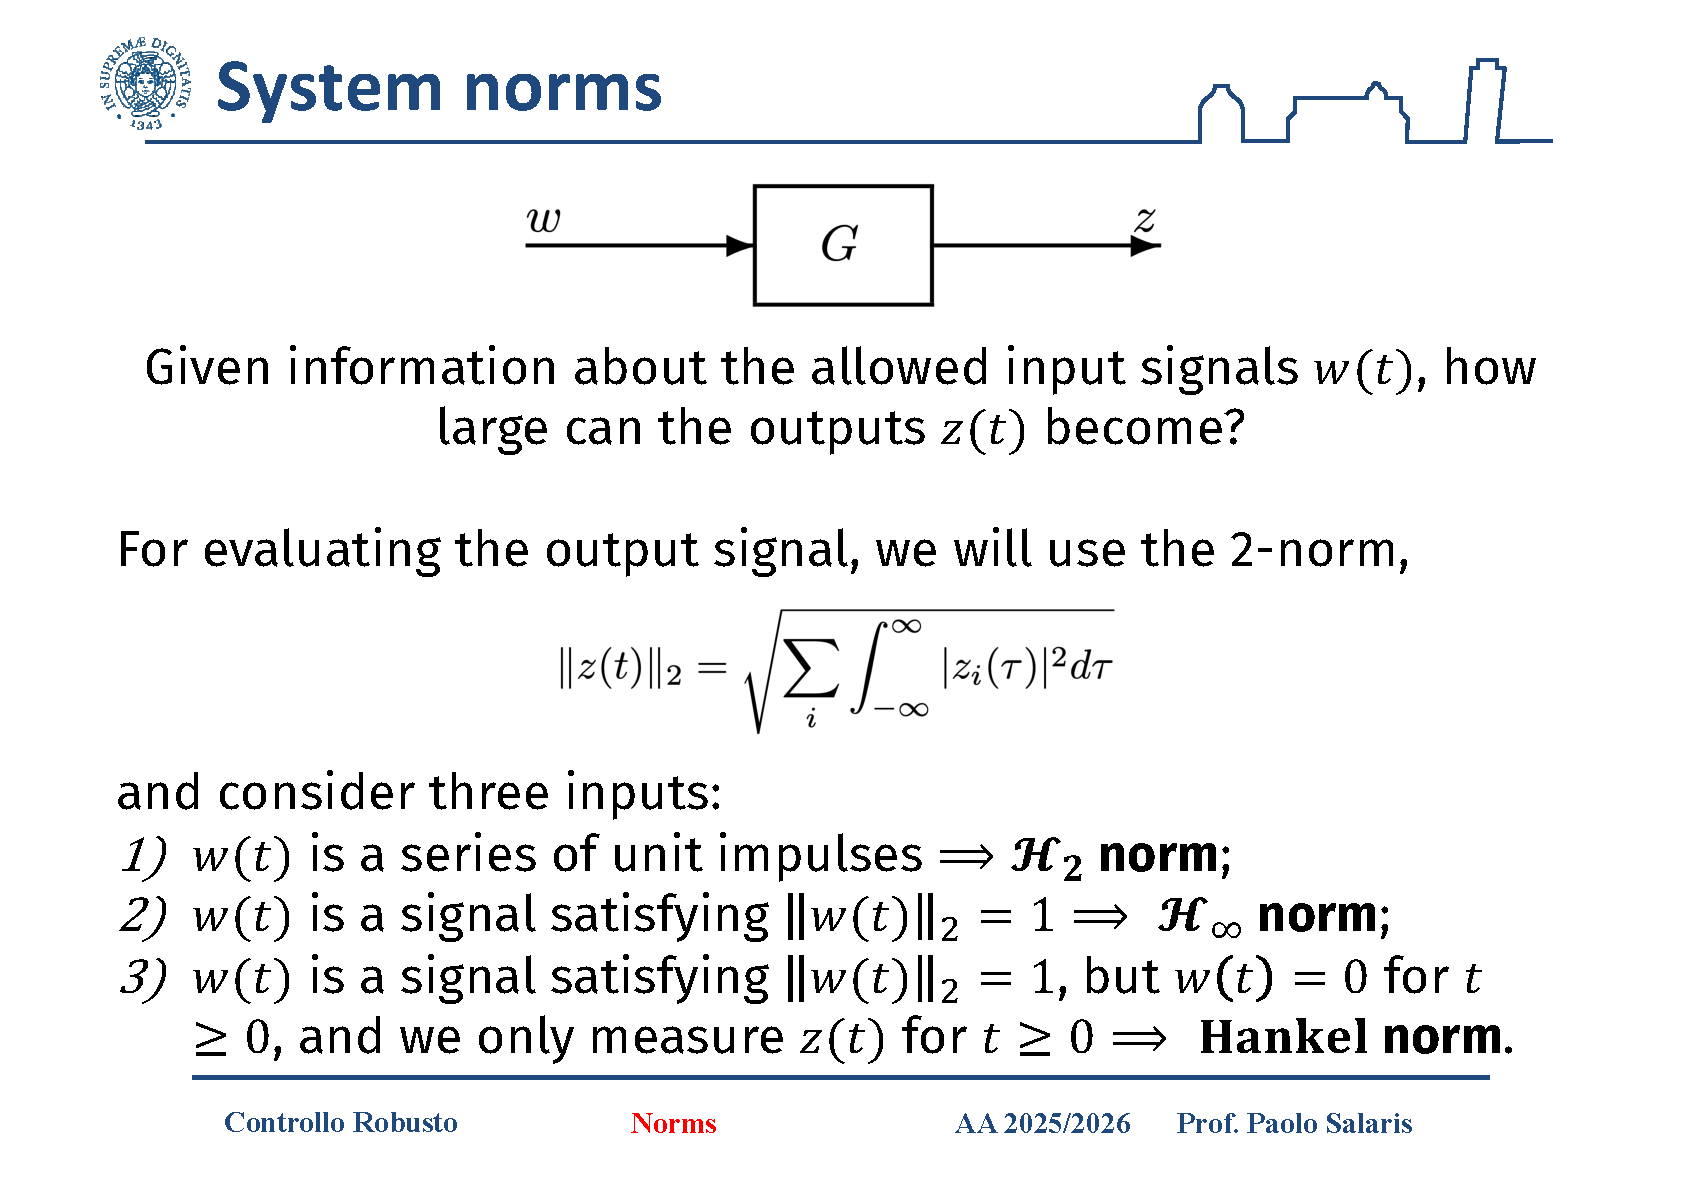
\includegraphics[width=0.78\textwidth]{images6/norms-11-32-005.png}
\vfill
\begin{focusbox}
\textbf{Obiettivo del documento.} Questa parte del testo sviluppa la Lezione 7 a partire dalle slide 11--32 del PDF ``Norms for signals and systems''. Il filo conduttore è il passaggio dalla misura della grandezza di un segnale alla misura della grandezza di un sistema dinamico. Dopo aver esteso la norma $L_2$ alle famiglie $L_p$ e $L_\infty$, la lezione introduce le norme di sistema, con particolare attenzione alla norma $H_2$: definizione nel tempo tramite risposta impulsiva, interpretazione in frequenza tramite Parseval, calcolo mediante residui e lettura stocastica come varianza di uscita a regime.
\end{focusbox}
\vfill
{\large Basato sulle slide del corso AA 2025/2026\par}
\end{coverpage}

\section{Lezione 7}

\subsection{Visione d'insieme della lezione}

La Lezione 7 prosegue in modo molto naturale il lavoro svolto nella Lezione 6. L\`i ci si era fermati alla norma $L_2$ dei segnali, al teorema di Parseval e al calcolo tramite residui. Qui il quadro viene completato in due direzioni. La prima consiste nell'allargare la famiglia delle norme considerate, introducendo le norme $L_p$ e soprattutto la norma $L_\infty$, che misura il picco massimo di un segnale invece della sua energia complessiva. La seconda, ancora pi\`u importante per il controllo robusto, consiste nel passare dalle norme dei segnali alle norme dei sistemi.

Questo passaggio \`e cruciale perch\'e in progettazione non basta sapere come misurare un ingresso o un'uscita separatamente: bisogna capire come un sistema trasforma segnali ammessi in segnali risultanti. In altre parole, si vuole rispondere a una domanda del tipo: dato un certo insieme di ingressi possibili, qual \`e la massima grandezza che l'uscita pu\`o assumere? Le norme di sistema nascono precisamente per dare una risposta rigorosa a questa domanda.

Le slide 11--32 del PDF sulle norme sono costruite attorno a questo snodo concettuale. Le prime chiariscono il significato di $L_p$ e di $L_\infty$ per segnali scalari e vettoriali. Le successive introducono il problema delle norme di sistema e mostrano che, se l'ingresso ammesso \`e una sequenza di impulsi unitari, si ottiene la norma $H_2$. Da qui la lezione sviluppa tre modi equivalenti di leggere la norma $H_2$: come energia della risposta impulsiva, come potenza spettrale totale e come varianza di uscita nel caso di rumore bianco.

\begin{keybox}
Il messaggio centrale della lezione \`e che una norma di sistema non misura semplicemente ``quanto \`e grande'' una matrice di trasferimento, ma quantifica quanto il sistema pu\`o amplificare segnali appartenenti a una certa classe. La scelta della classe di ingressi ammessi determina il tipo di norma e quindi il significato prestazionale della misura.
\end{keybox}

\subsection{Norme \texorpdfstring{$L_p$}{Lp} e \texorpdfstring{$L_\infty$}{Linf} dei segnali}

Le prime slide del blocco riprendono la norma $L_2$ introdotta nella lezione precedente e la collocano dentro una famiglia pi\`u ampia. Per un segnale scalare $v(t)$ definito per $t\ge 0$, la norma $L_p$ si definisce come
$$
\|v\|_{L_p}
=
\left(\int_0^\infty |v(t)|^p\,dt\right)^{1/p},
\qquad 1\le p < \infty.
$$
Nel caso particolare $p=1$ si ottiene
$$
\|v\|_{L_1}=\int_0^\infty |v(t)|\,dt,
$$
cio\`e l'area assoluta sottesa dal segnale. Gi\`a questa semplice osservazione fa vedere che cambiare norma non significa cambiare solo una formula: significa cambiare il criterio con cui si aggrega l'informazione nel tempo.

Nel caso $p=2$ si recupera la norma energetica gi\`a vista. La slide sottolinea per\`o un punto importante: per $p\neq 2$ non esiste, in generale, una relazione altrettanto semplice e potente del teorema di Parseval che colleghi direttamente la norma del segnale nel tempo e una norma equivalente nel dominio di Laplace o di Fourier. La norma $L_2$ \`e speciale proprio perch\'e gode di questa perfetta corrispondenza con l'energia spettrale.

Le slide ricordano anche il significato della lettera $L$: si tratta dello spazio di funzioni Lebesgue-integrabili, quindi di una generalizzazione del quadro riemanniano classico. Dal punto di vista pratico, il messaggio da trattenere \`e che le norme di segnale richiedono una nozione di integrabilit\`a abbastanza flessibile da includere anche classi di segnali utili in analisi e controllo.

\begin{figure}[H]
    \centering
    \begin{subfigure}{0.48\textwidth}
        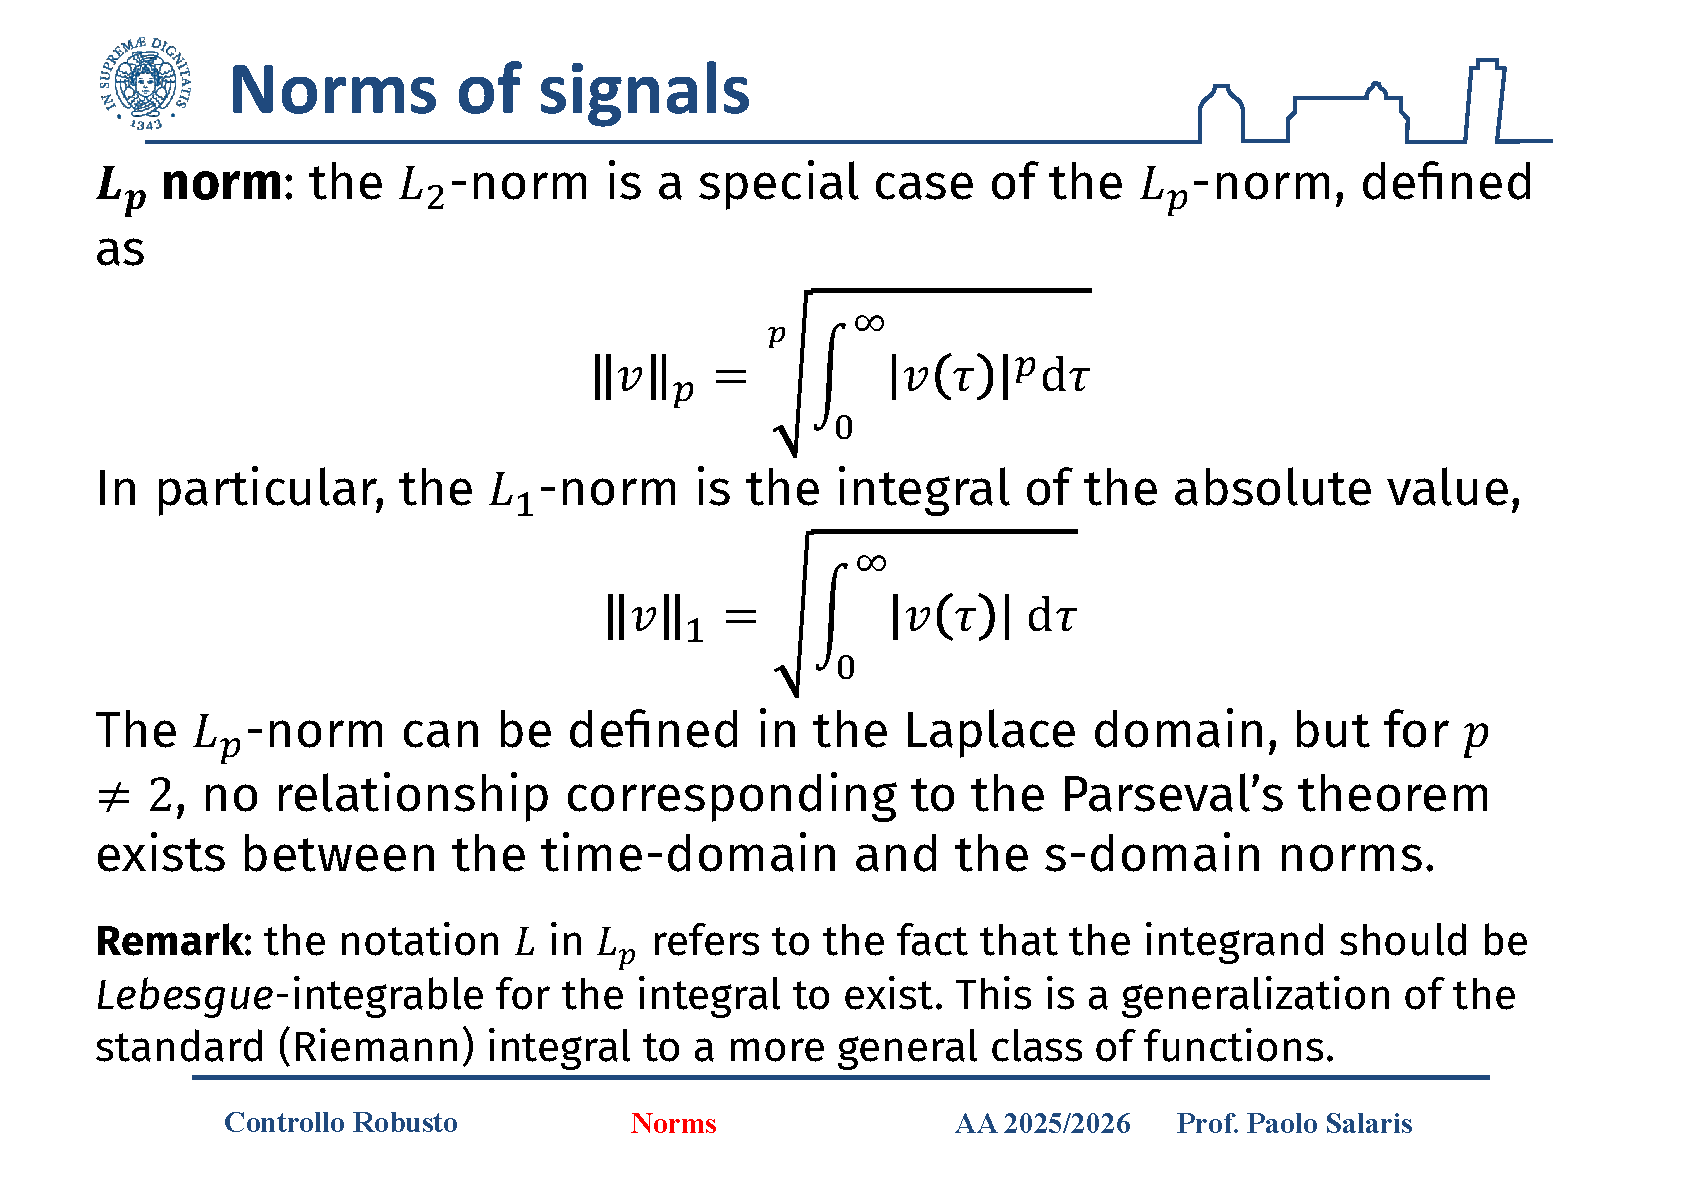
\includegraphics[width=\linewidth]{images6/norms-11-32-001.png}
        \caption{Generalizzazione dalla norma $L_2$ alla famiglia delle norme $L_p$.}
    \end{subfigure}
    \hfill
    \begin{subfigure}{0.48\textwidth}
        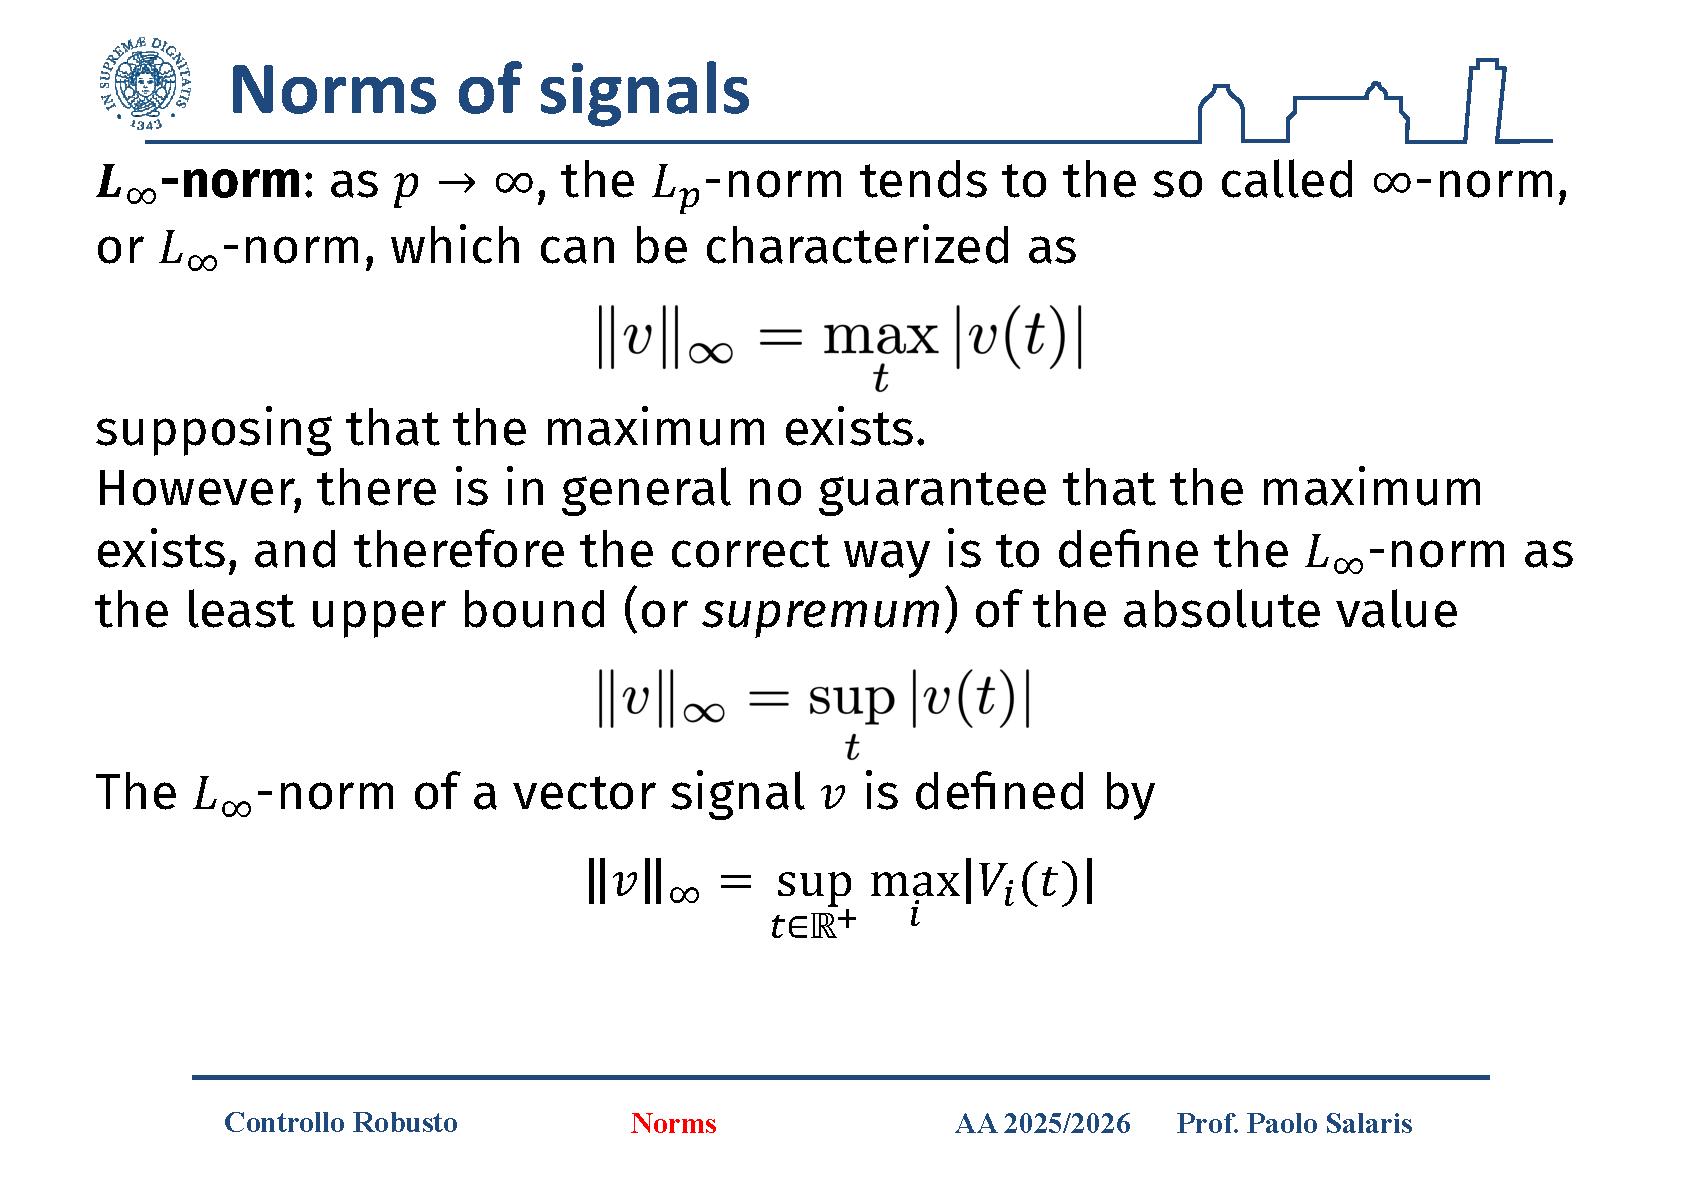
\includegraphics[width=\linewidth]{images6/norms-11-32-002.png}
        \caption{Definizione di norma $L_\infty$ come estremo superiore del modulo del segnale.}
    \end{subfigure}
    \caption{Le norme $L_p$ misurano grandezze diverse dello stesso segnale: massa assoluta, energia, picco massimo.}
\end{figure}

\subsubsection{Perch\'e in \texorpdfstring{$L_\infty$}{Linf} compare il supremum}

Quando $p\to\infty$, la norma $L_p$ tende alla norma di picco:
$$
\|v\|_{L_\infty}=\sup_{t\ge 0}|v(t)|.
$$
Le slide osservano giustamente che sarebbe pi\`u intuitivo scrivere un massimo, ma in generale non si pu\`o garantire che il massimo venga effettivamente raggiunto. Per questo la definizione corretta usa il \emph{supremum}, cio\`e il minimo maggiorante.

Questo punto non \`e un dettaglio pedante. In controllo robusto si lavora spesso con segnali o risposte in frequenza che possono avvicinarsi arbitrariamente a un valore senza raggiungerlo esattamente. Se si usasse solo il massimo, molte formule non sarebbero stabili dal punto di vista matematico. Il supremum, invece, permette di parlare in modo rigoroso del peggior caso anche quando il peggior caso non si realizza in un punto preciso ma solo come limite.

Per un segnale vettoriale $v(t)\in\mathbb{R}^m$ la definizione diventa
$$
\|v\|_{L_\infty}
=
\sup_{t\ge 0}\max_{1\le i\le m}|v_i(t)|.
$$
La norma di picco di un segnale multi-canale seleziona quindi, in ogni istante, il canale pi\`u grande in valore assoluto e poi guarda il peggiore tra tutti gli istanti. \`E una misura molto severa, ma proprio per questo \`e adatta a esprimere specifiche del tipo ``nessuna componente dell'uscita deve superare una certa soglia''.

Le slide riportano anche l'esempio della funzione che si avvicina a $1$ senza mai toccarlo, per chiarire la differenza tra massimo e supremum. Gli esempi finali con $x(t)=e^{-t}$ e con il vettore
$$
x(t)=
\begin{bmatrix}
e^{-t}\\
e^{-2t}
\end{bmatrix}
$$
mostrano che in entrambi i casi la norma $L_\infty$ vale $1$, perch\'e il picco si ha in $t=0$.

\begin{figure}[H]
    \centering
    \begin{subfigure}{0.48\textwidth}
        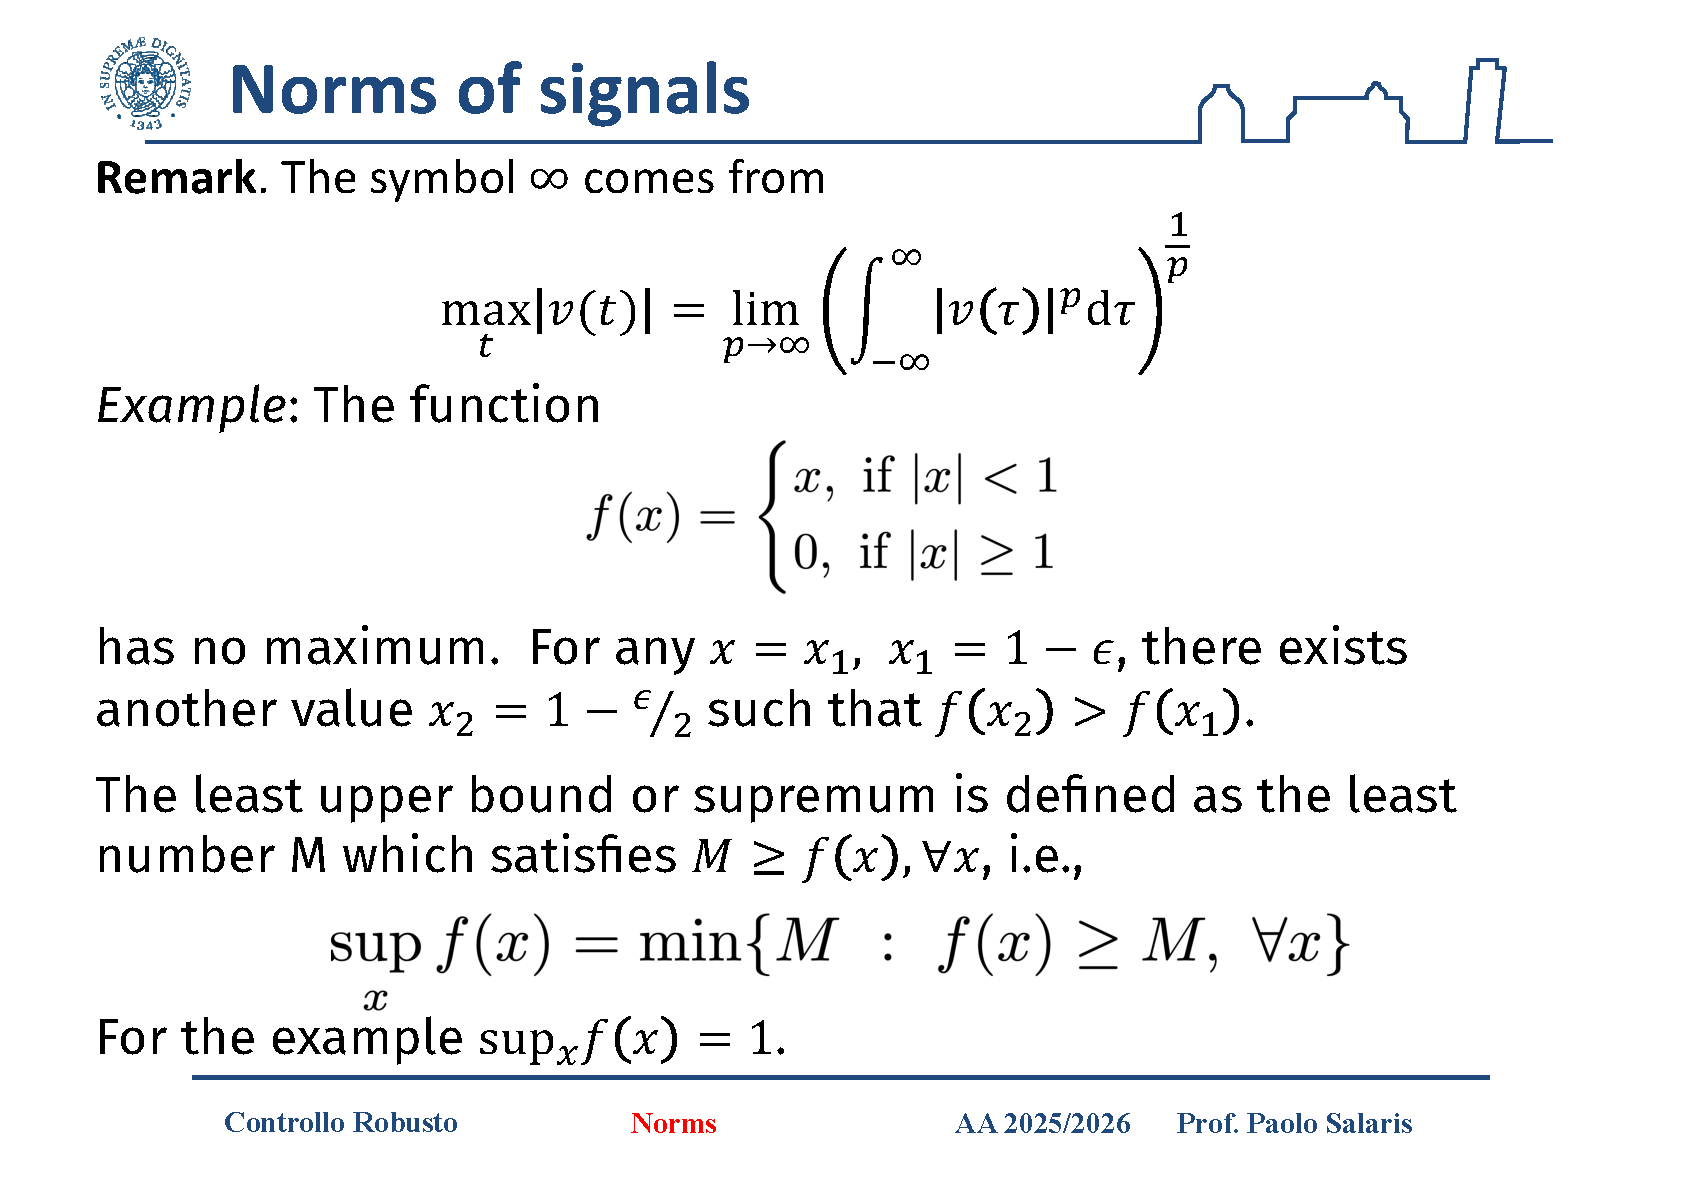
\includegraphics[width=\linewidth]{images6/norms-11-32-003.png}
        \caption{Spiegazione del concetto di supremum e motivo per cui il massimo pu\`o non esistere.}
    \end{subfigure}
    \hfill
    \begin{subfigure}{0.48\textwidth}
        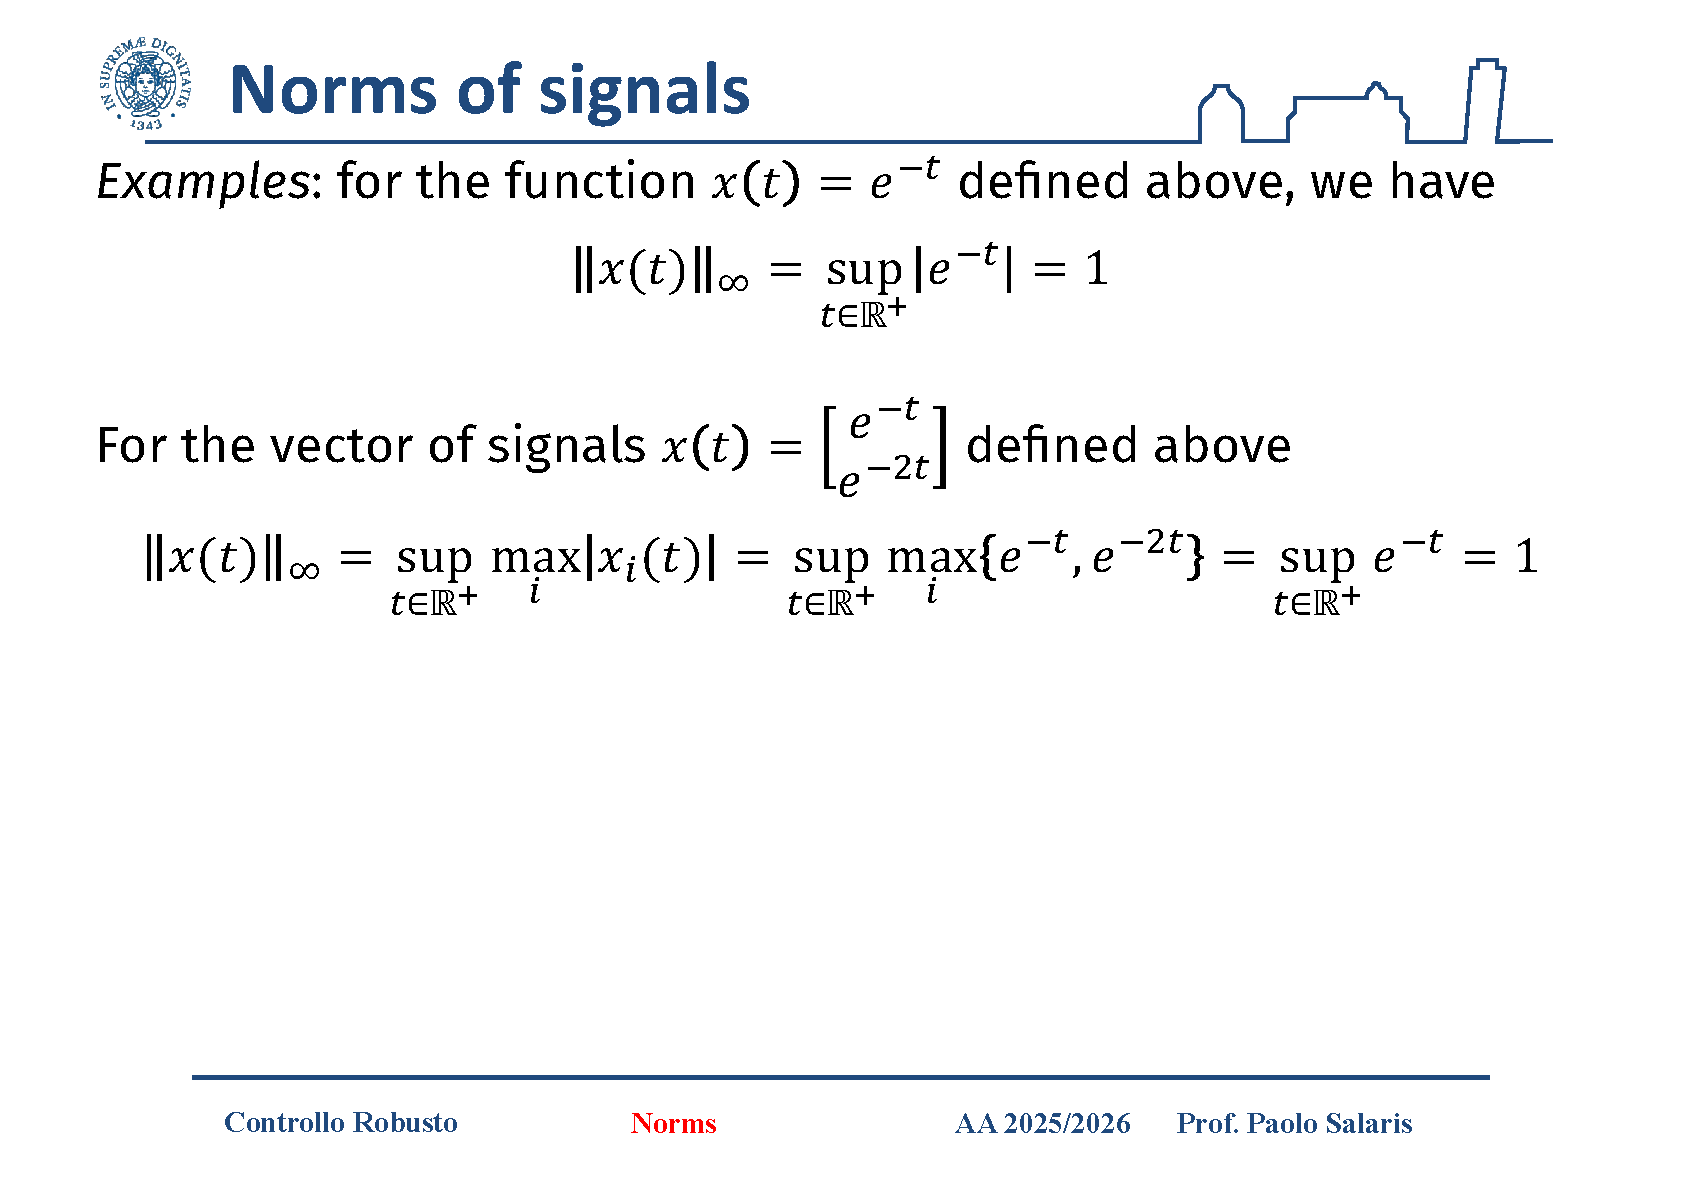
\includegraphics[width=\linewidth]{images6/norms-11-32-004.png}
        \caption{Esempi immediati di calcolo della norma $L_\infty$ per segnali scalari e vettoriali.}
    \end{subfigure}
    \caption{La norma $L_\infty$ cattura il valore di picco del segnale ed \`e quindi una misura di tipo worst-case.}
\end{figure}

\begin{focusbox}
\textbf{Confronto concettuale utile.} La norma $L_2$ risponde alla domanda ``quanta energia complessiva porta il segnale?'', mentre la norma $L_\infty$ risponde alla domanda ``qual \`e il valore pi\`u grande che il segnale pu\`o assumere?''. In controllo queste due domande corrispondono a due famiglie diverse di specifiche.
\end{focusbox}

\subsection{Dalle norme dei segnali alle norme di sistema}

La slide successiva contiene il vero cambio di passo della lezione. Si considera un sistema $G$ che trasforma un ingresso $w(t)$ in un'uscita $z(t)$ e si pone la domanda fondamentale:
\begin{center}
\emph{dato un insieme di ingressi ammessi, quanto grande pu\`o diventare l'uscita?}
\end{center}
Il punto essenziale \`e che il sistema non viene pi\`u osservato come oggetto statico, ma come operatore che associa un segnale a un altro segnale. Una norma di sistema misura la capacit\`a di questo operatore di amplificare certi ingressi.

Nella slide l'uscita viene misurata con la norma $2$, mentre si distinguono tre classi di ingressi:
\begin{itemize}
    \item una successione di impulsi unitari applicati ai vari canali di ingresso, che conduce alla norma $H_2$;
    \item segnali a energia unitaria, $\|w\|_2=1$, che conducono alla norma $H_\infty$ intesa come massimo guadagno indotto;
    \item segnali a energia unitaria confinati nel passato, con uscita osservata nel futuro, che conducono alla norma di Hankel.
\end{itemize}

Questa classificazione \`e molto istruttiva perch\'e fa vedere che le norme di sistema non sono arbitrarie. Ognuna nasce da una diversa domanda ingegneristica:
\begin{itemize}
    \item come reagisce il sistema a eccitazioni impulsive?
    \item qual \`e la massima amplificazione su ingressi energeticamente limitati?
    \item quanta informazione o energia passa dal passato al futuro del sistema?
\end{itemize}

In questa lezione il corso sviluppa soprattutto il primo caso, cio\`e la norma $H_2$. Le altre due vengono solo richiamate per mostrare l'architettura generale del tema.

\begin{figure}[H]
    \centering
    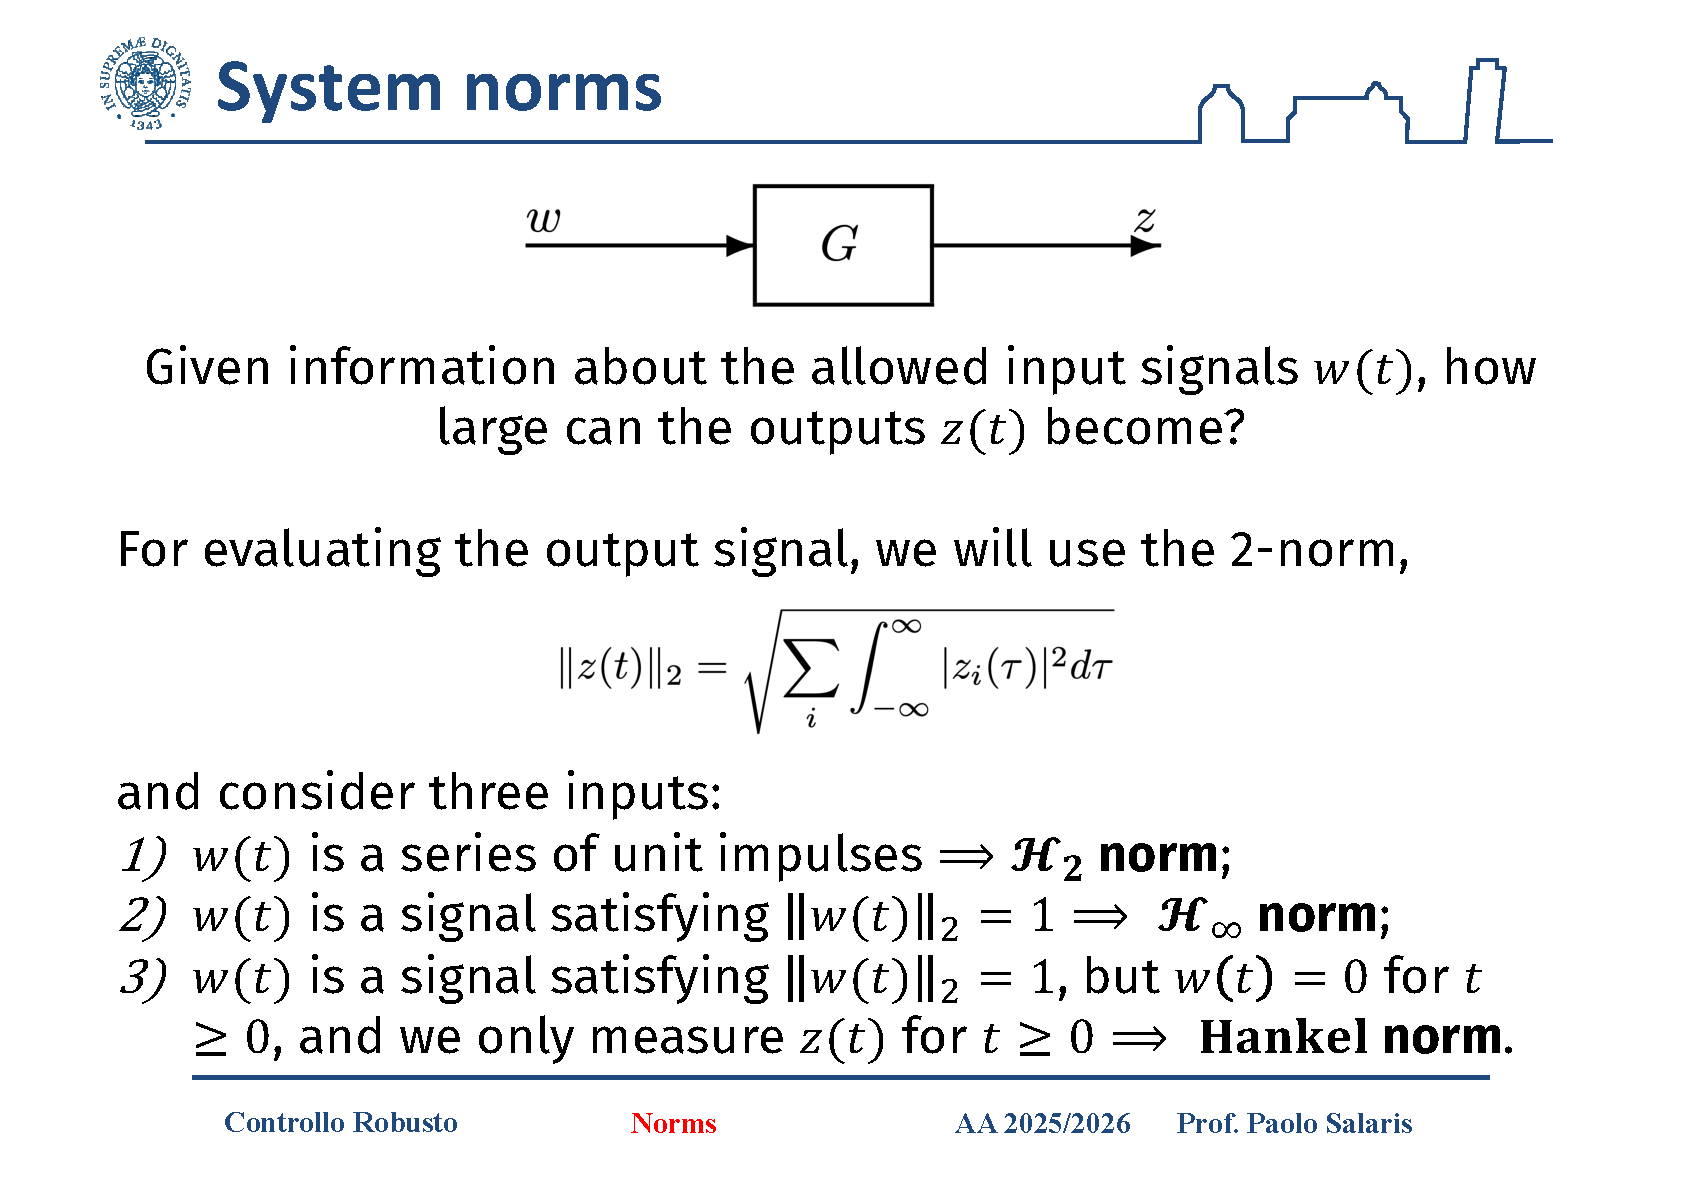
\includegraphics[width=0.82\textwidth]{images6/norms-11-32-005.png}
    \caption{Le norme di sistema nascono scegliendo una classe di ingressi ammessi e misurando la grandezza dell'uscita risultante.}
\end{figure}

\subsection{Lo spazio di Hardy \texorpdfstring{$H_2$}{H2}}

Prima di definire operativamente la norma $H_2$ delle matrici di trasferimento, le slide introducono il contesto funzionale in cui essa vive: lo spazio di Hardy $H_2$. In forma astratta, esso raccoglie funzioni analitiche nel semipiano aperto considerato dalla convenzione adottata e tali che
$$
\|f\|_{H_2}^2
=
\sup_{a>0}\frac{1}{2\pi}\int_{-\infty}^{\infty}|f(a+j\omega)|^2\,d\omega
<
\infty.
$$
La frontiera naturale di questo spazio \`e l'asse immaginario, e la norma si pu\`o leggere come norma quadratica della traccia al bordo.

Le slide formulano questa definizione usando l'analiticit\`a nel semipiano destro. In controllo, per\`o, con la convenzione standard sulla variabile di Laplace si parla di sistemi stabili quando i poli stanno nel semipiano sinistro. Non c'\`e una contraddizione sostanziale: si tratta di una differenza di convenzione nella variabile complessa. Operativamente, nel corso si usa il nome $H_2$ per indicare l'insieme delle matrici di trasferimento stabili e strettamente proprie la cui energia spettrale \`e finita.

Questa precisazione \`e importante perch\'e evita un fraintendimento frequente: la norma $H_2$ non \`e una qualunque norma su matrici costanti, ma una norma su funzioni di trasferimento, cio\`e su oggetti dinamici. La richiesta di stretta properness garantisce che l'integrale in frequenza converga alle alte frequenze, mentre la stabilit\`a garantisce che la risposta impulsiva sia sufficientemente regolare da avere energia finita.

\begin{figure}[H]
    \centering
    \begin{subfigure}{0.48\textwidth}
        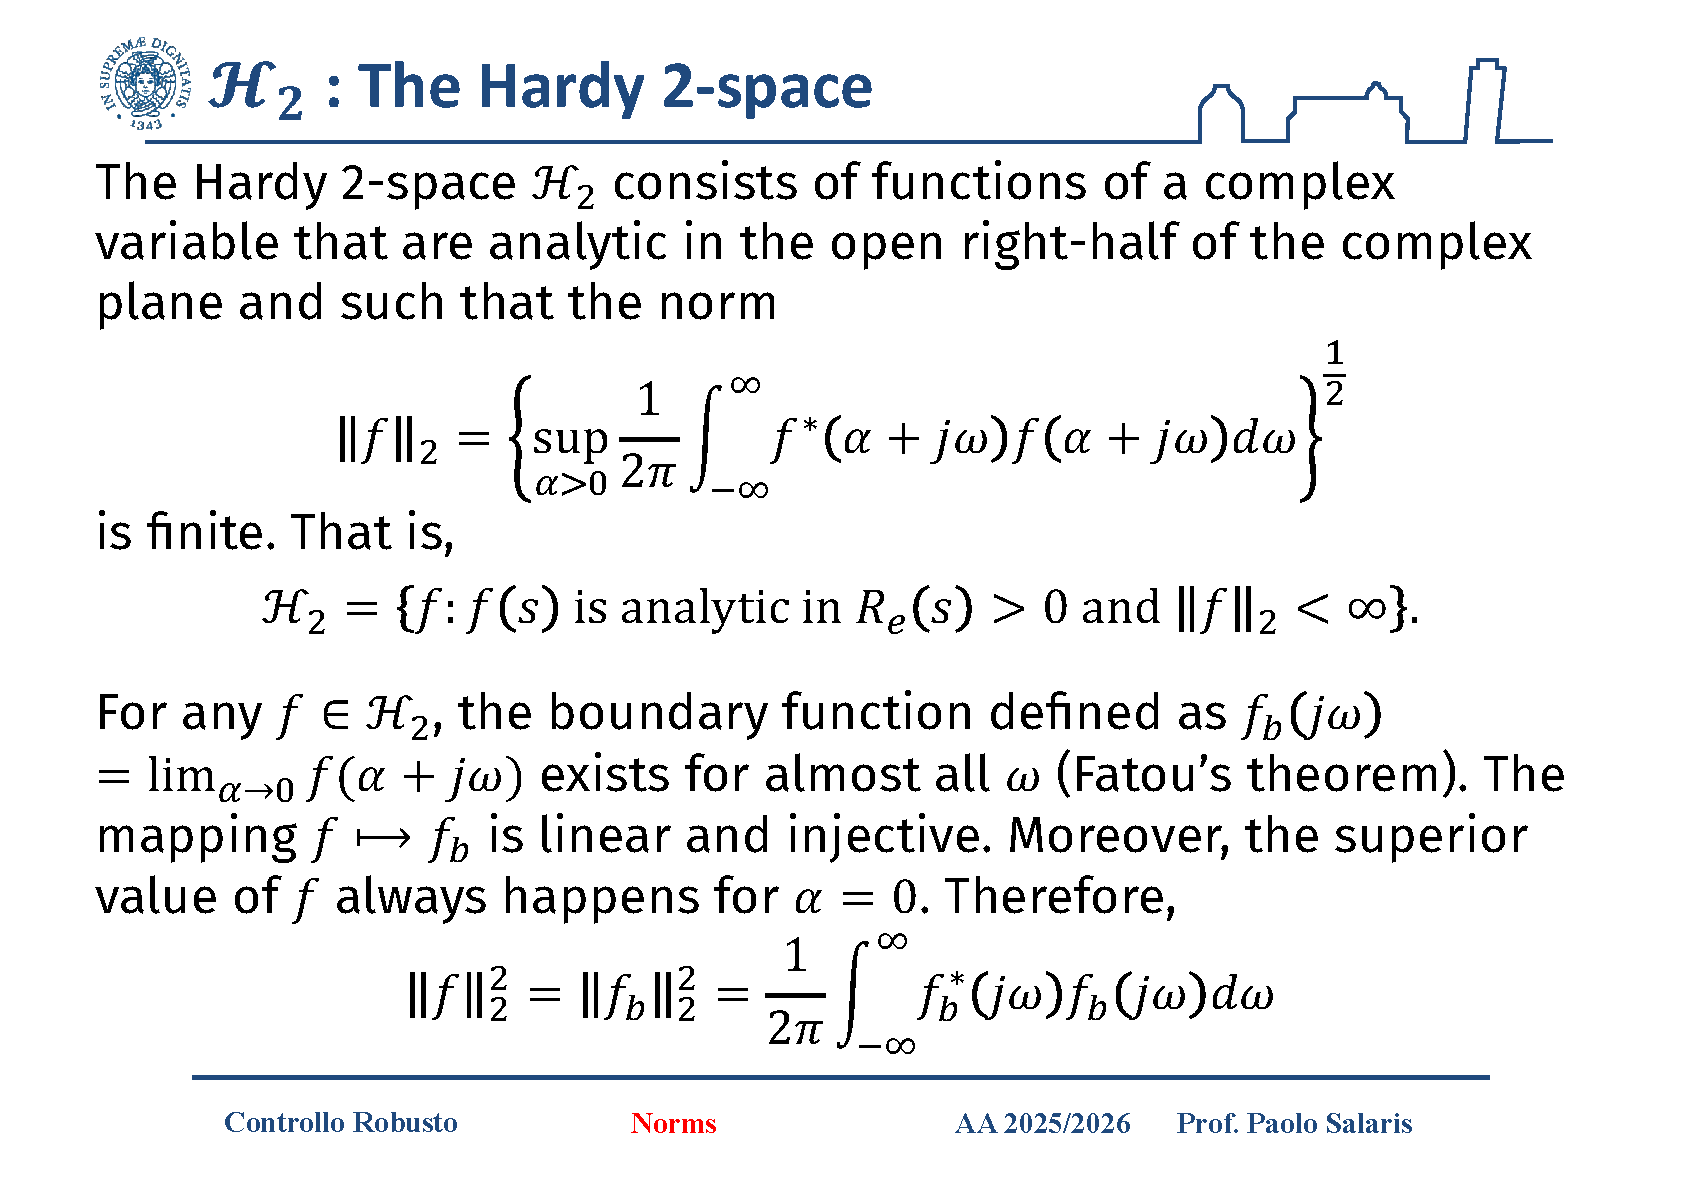
\includegraphics[width=\linewidth]{images6/norms-11-32-006.png}
        \caption{Definizione astratta dello spazio di Hardy $H_2$ e norma al bordo.}
    \end{subfigure}
    \hfill
    \begin{subfigure}{0.48\textwidth}
        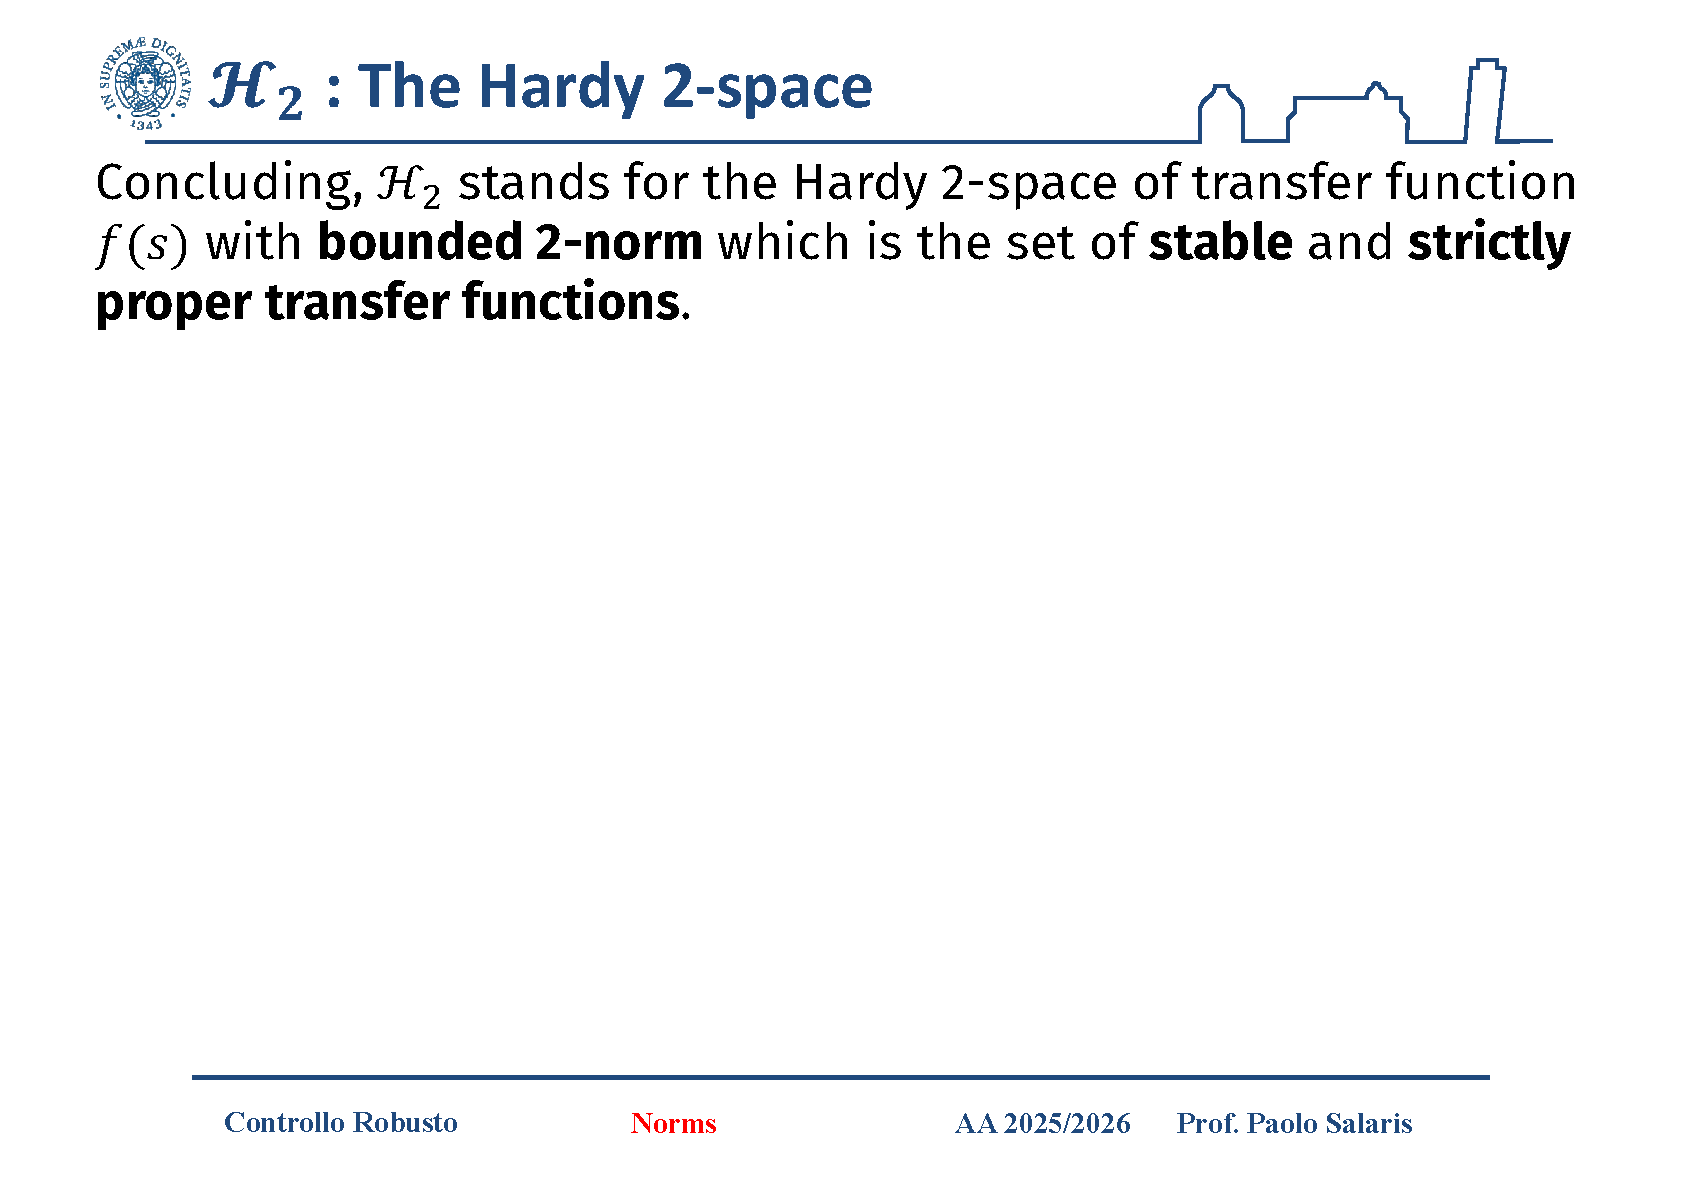
\includegraphics[width=\linewidth]{images6/norms-11-32-007.png}
        \caption{Interpretazione pratica: nel corso $H_2$ coincide con il mondo dei trasferimenti stabili e strettamente propri.}
    \end{subfigure}
    \caption{La definizione funzionale di $H_2$ prepara il collegamento tra risposta impulsiva, energia e integrali frequenziali.}
\end{figure}

\subsection{Norma \texorpdfstring{$H_2$}{H2} di sistemi stabili}

\subsubsection{Definizione nel dominio del tempo}

Sia $G(s)$ una matrice di trasferimento stabile e strettamente propria, e sia $g(t)$ la sua risposta impulsiva. Per evitare ambiguit\`a con la norma $L_2$ dei segnali, nel testo useremo la scrittura $\|G\|_{H_2}$, anche se nelle slide compare spesso semplicemente $\|G\|_2$.

Per sistemi SISO o SIMO la definizione \`e diretta: la norma $H_2$ \`e la norma $L_2$ della risposta impulsiva. Per sistemi MIMO, invece, bisogna sommare il contributo di tutti i canali di ingresso. Se si scrive la risposta impulsiva per colonne,
$$
g(t)=
\begin{bmatrix}
g_1(t) & \cdots & g_m(t)
\end{bmatrix},
$$
dove $g_i(t)$ \`e la risposta di uscita all'impulso unitario applicato al canale di ingresso $i$-esimo, allora
$$
\|G\|_{H_2}^2
=
\sum_{i=1}^{m}\int_0^\infty \|g_i(t)\|_2^2\,dt
=
\int_0^\infty \operatorname{tr}\!\bigl(g(t)g^T(t)\bigr)\,dt.
$$

Questa formula \`e estremamente importante. Dice che la norma $H_2$ misura l'energia totale delle risposte impulsive che il sistema produce quando si eccitano, uno alla volta, tutti i canali di ingresso. In termini di singoli elementi della matrice di trasferimento si pu\`o scrivere anche
$$
\|G\|_{H_2}^2
=
\sum_{i,j}\|g_{ij}\|_{L_2}^2,
$$
cio\`e la somma delle energie di tutte le funzioni impulsive ingresso-uscita.

\begin{figure}[H]
    \centering
    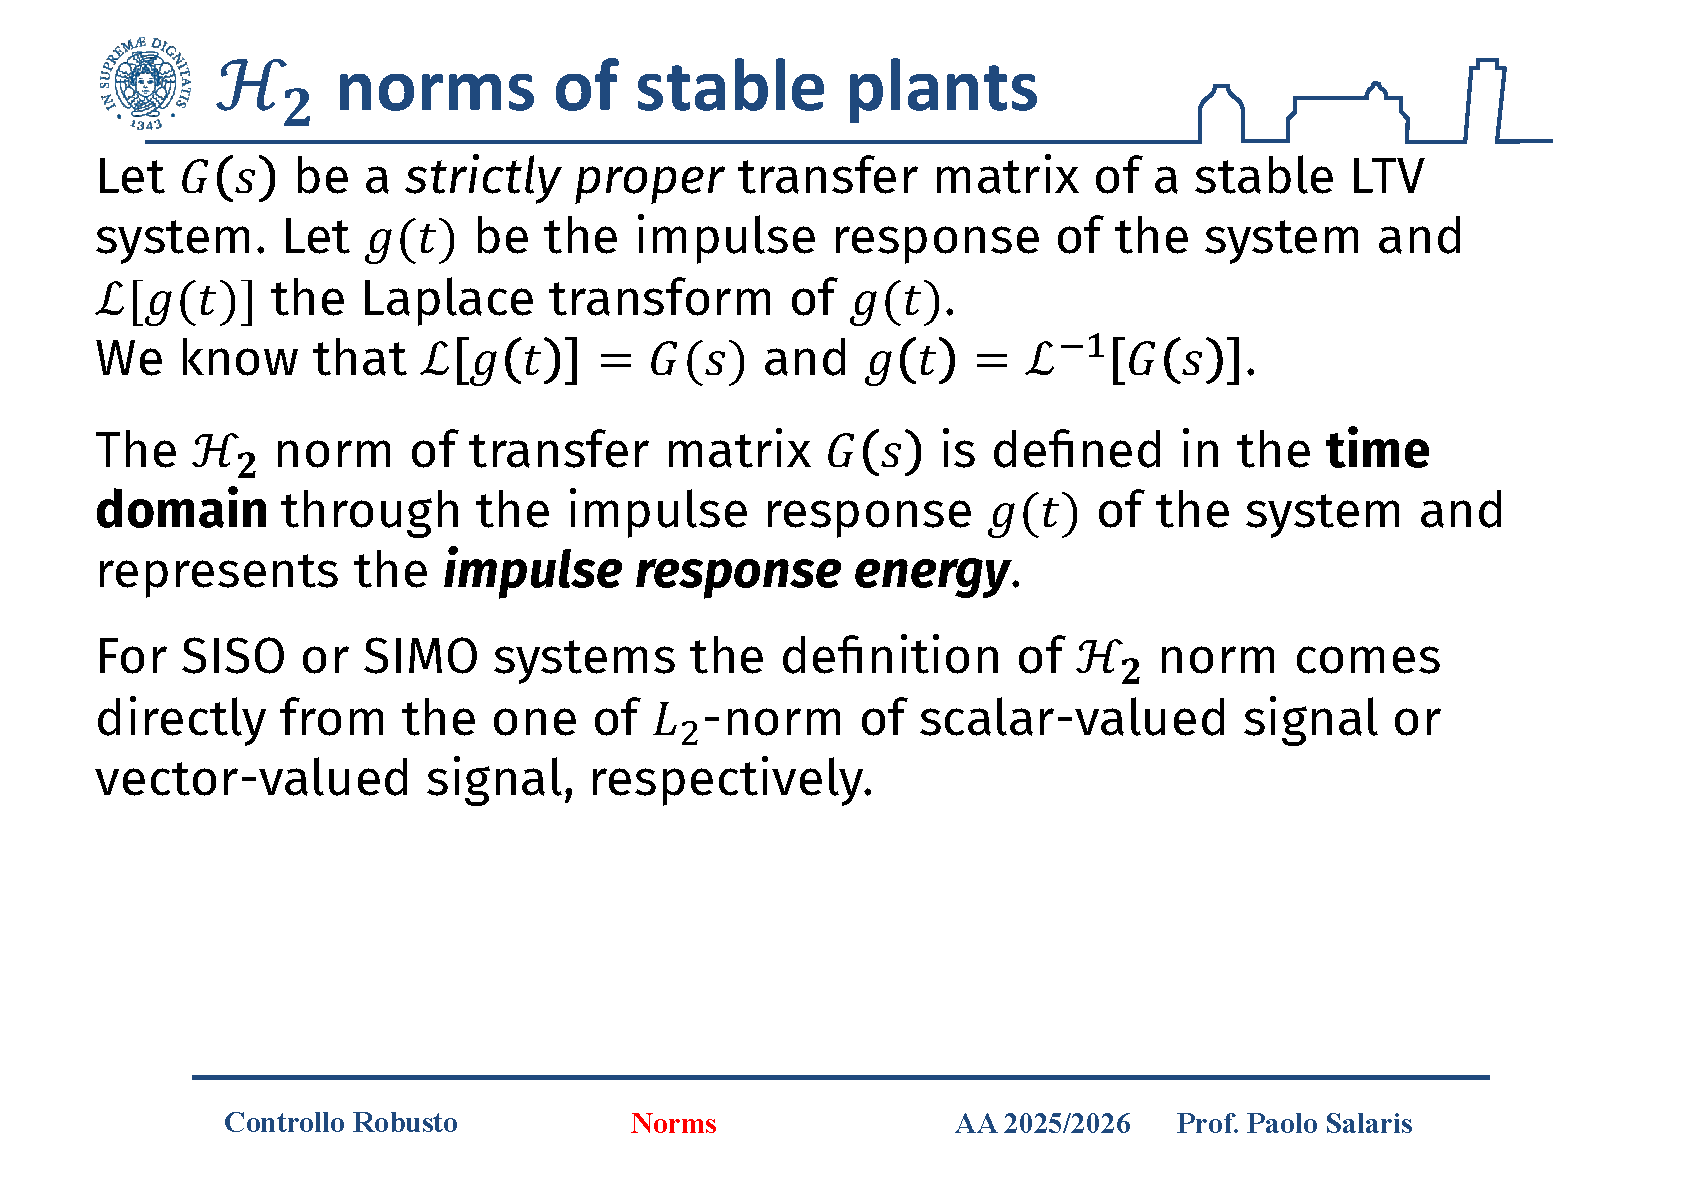
\includegraphics[width=0.78\textwidth]{images6/norms-11-32-008.png}
    \caption{La norma $H_2$ nasce come energia della risposta impulsiva di un sistema stabile e strettamente proprio.}
\end{figure}

\begin{figure}[H]
    \centering
    \begin{subfigure}{0.48\textwidth}
        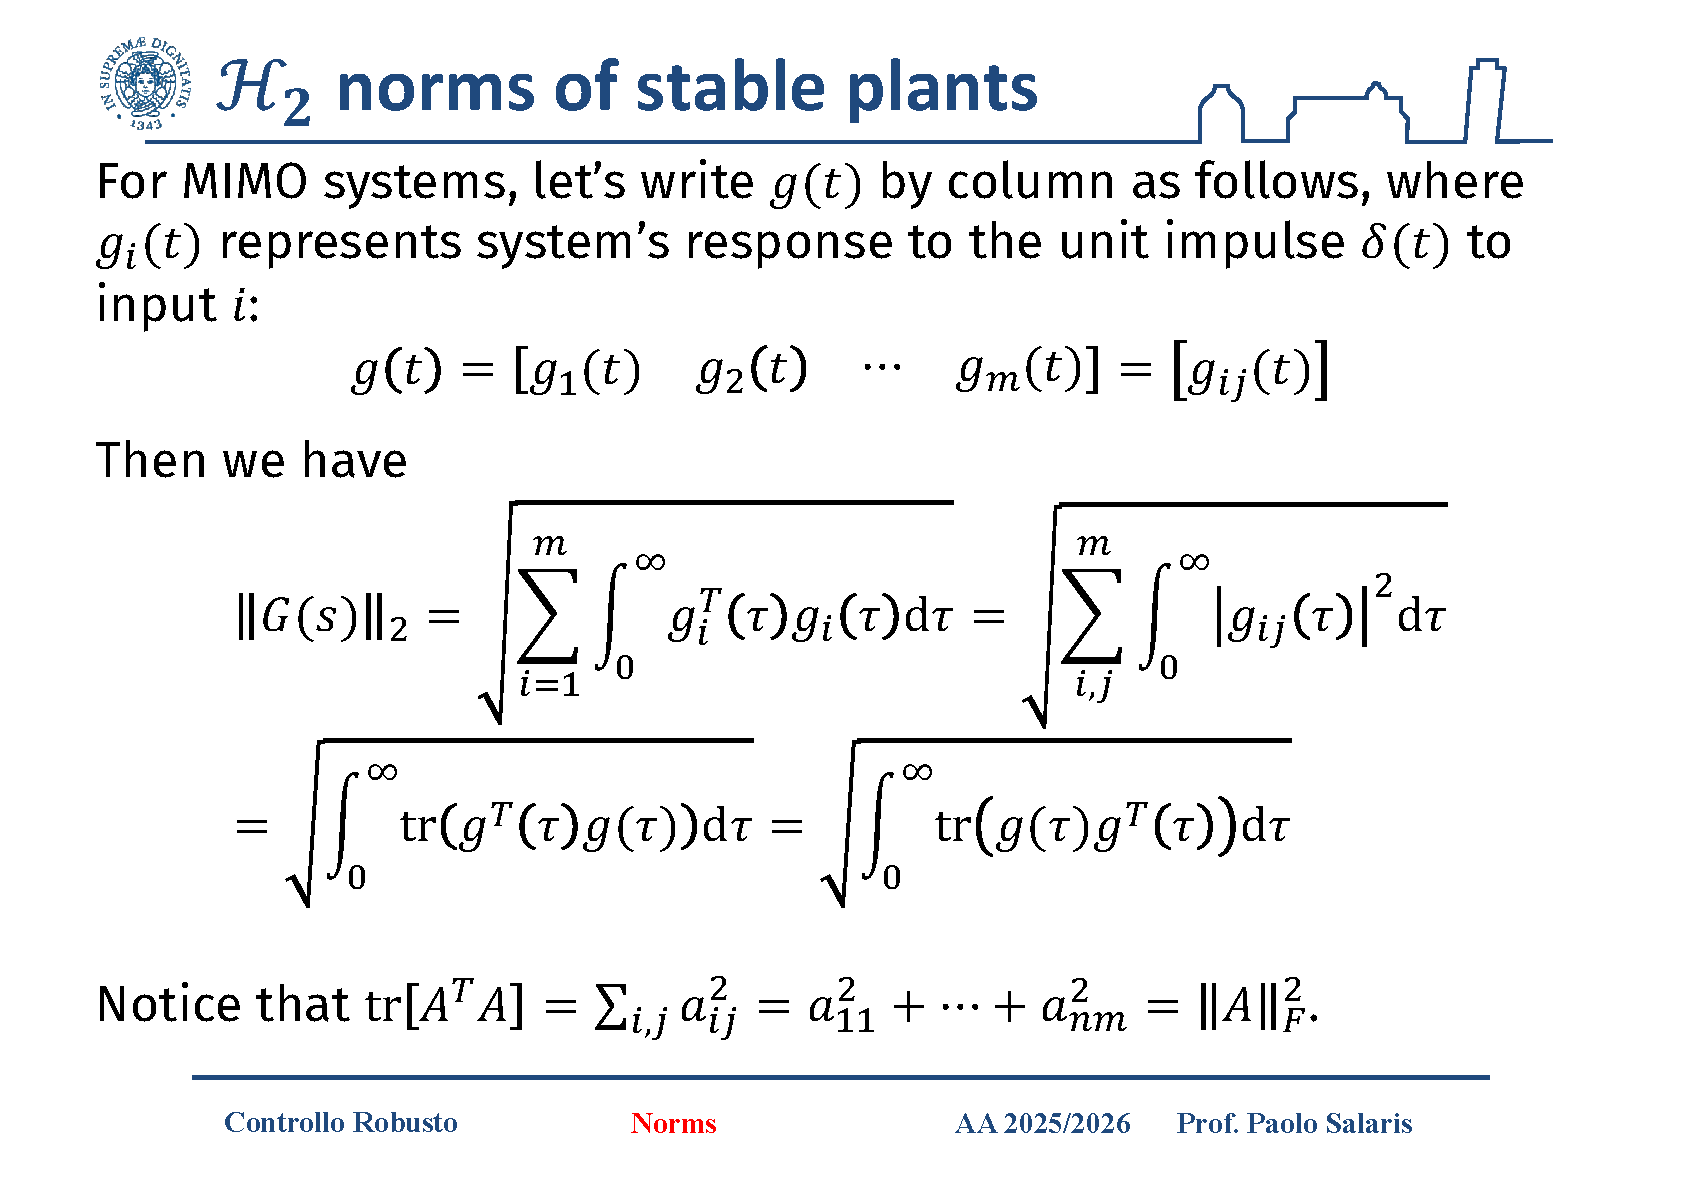
\includegraphics[width=\linewidth]{images6/norms-11-32-009.png}
        \caption{Definizione MIMO tramite colonne della risposta impulsiva e traccia di $g(t)g^T(t)$.}
    \end{subfigure}
    \hfill
    \begin{subfigure}{0.48\textwidth}
        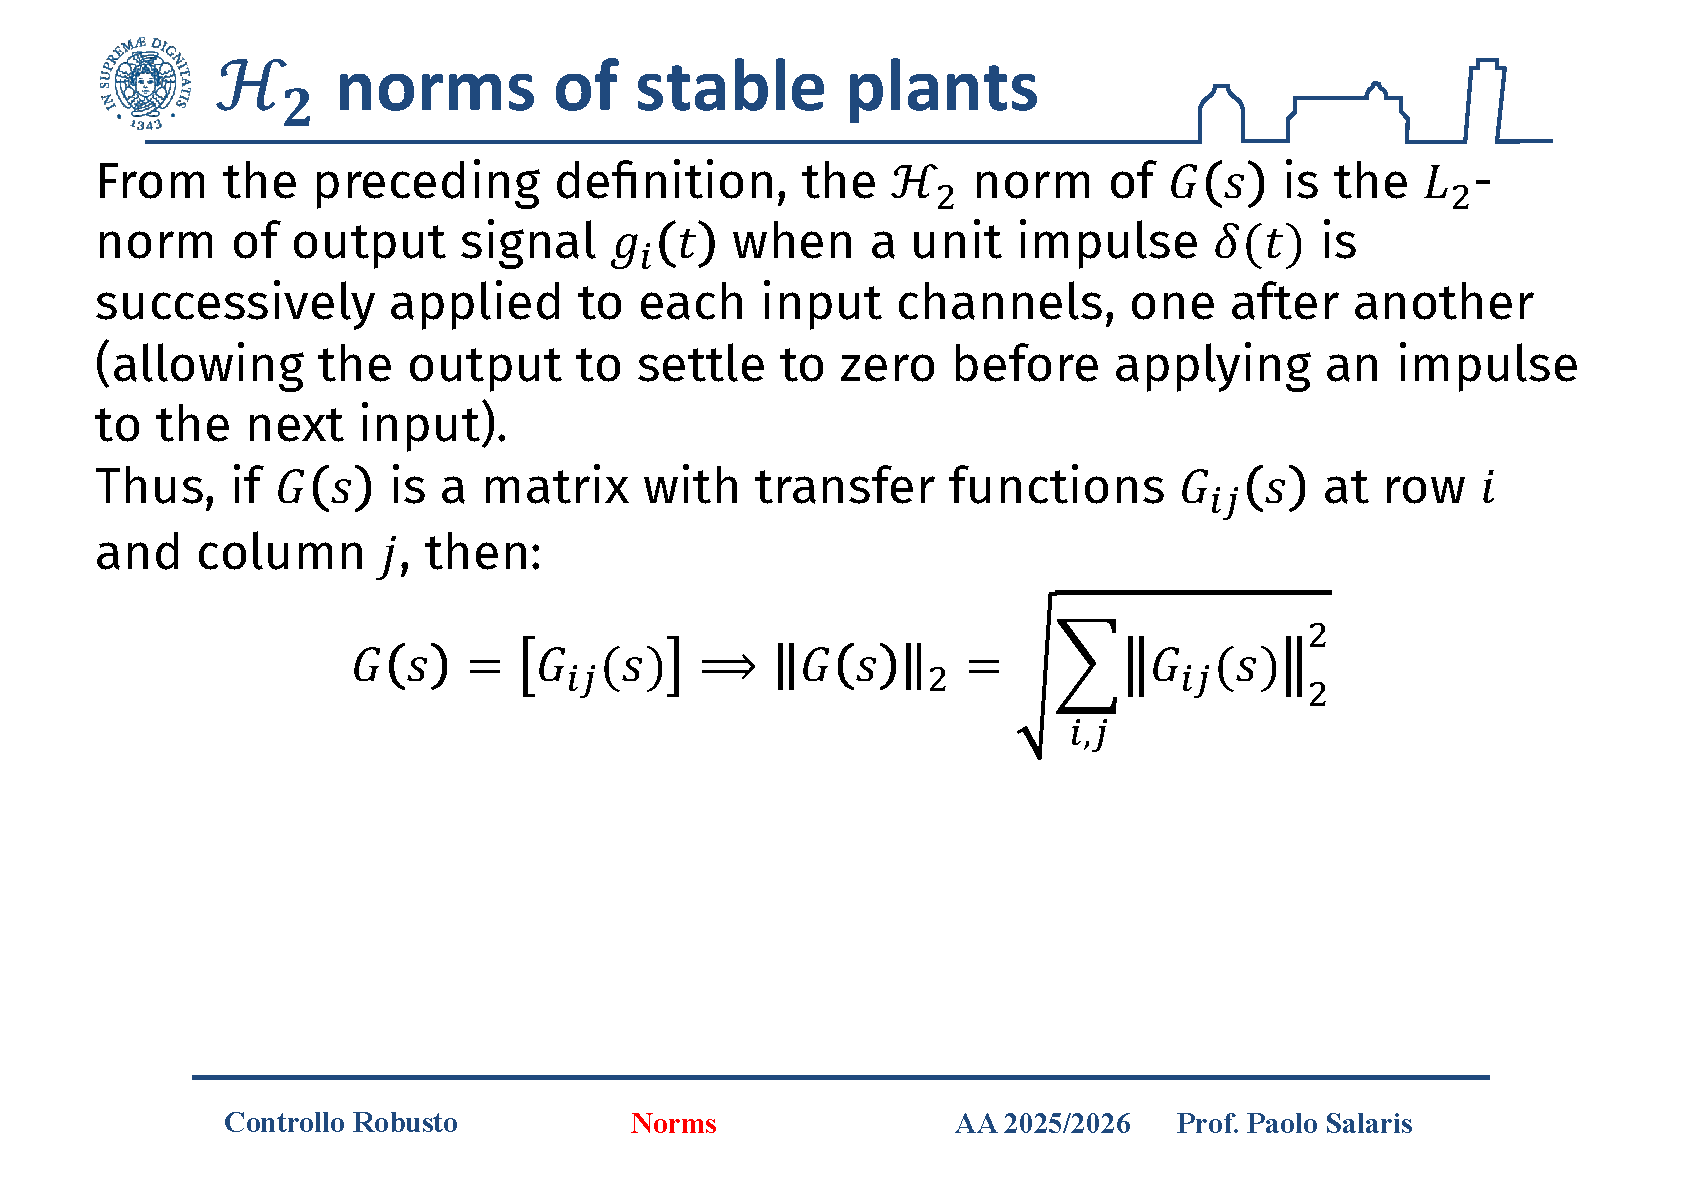
\includegraphics[width=\linewidth]{images6/norms-11-32-010.png}
        \caption{Interpretazione operativa: impulsi unitari applicati ai canali di ingresso uno dopo l'altro.}
    \end{subfigure}
    \caption{Per un sistema MIMO la norma $H_2$ aggrega l'energia di tutte le risposte impulsive parziali.}
\end{figure}

\begin{focusbox}
\textbf{Interpretazione pratica.} Una piccola norma $H_2$ significa che il sistema, mediamente, non disperde molta energia quando viene colpito da impulsi unitari. Per questo l'$H_2$ \`e una misura naturale di ``reattivit\`a energetica'' del sistema.
\end{focusbox}

\subsubsection{Definizione nel dominio della frequenza}

Grazie al teorema di Parseval, la stessa quantit\`a pu\`o essere espressa nel dominio della frequenza:
$$
\|G\|_{H_2}^2
=
\frac{1}{2\pi}\int_{-\infty}^{\infty}
\operatorname{tr}\!\bigl(G(-j\omega)^T G(j\omega)\bigr)\,d\omega.
$$
Nel caso di sistemi reali questa scrittura coincide con l'uso del trasposto coniugato e pu\`o essere letta anche come integrale della densit\`a di potenza spettrale complessiva.

Per un sistema SISO, la formula diventa
$$
\|G\|_{H_2}^2
=
\frac{1}{2\pi}\int_{-\infty}^{\infty}|G(j\omega)|^2\,d\omega.
$$
Le slide osservano che, in questa forma, la norma $H_2$ pu\`o essere interpretata come un \emph{guadagno medio} distribuito su tutte le frequenze. Non \`e il massimo guadagno, come accadr\`a con l'$H_\infty$, ma una media quadratica pesata uniformemente lungo l'asse delle frequenze.

Questa lettura spiega bene la differenza tra le due norme che il corso metter\`a a confronto pi\`u avanti:
\begin{itemize}
    \item la norma $H_2$ privilegia una lettura energetica e media;
    \item la norma $H_\infty$ privilegia una lettura di picco e worst-case.
\end{itemize}
Entrambe sono fondamentali, ma descrivono aspetti diversi della stessa dinamica.

\begin{figure}[H]
    \centering
    \begin{subfigure}{0.48\textwidth}
        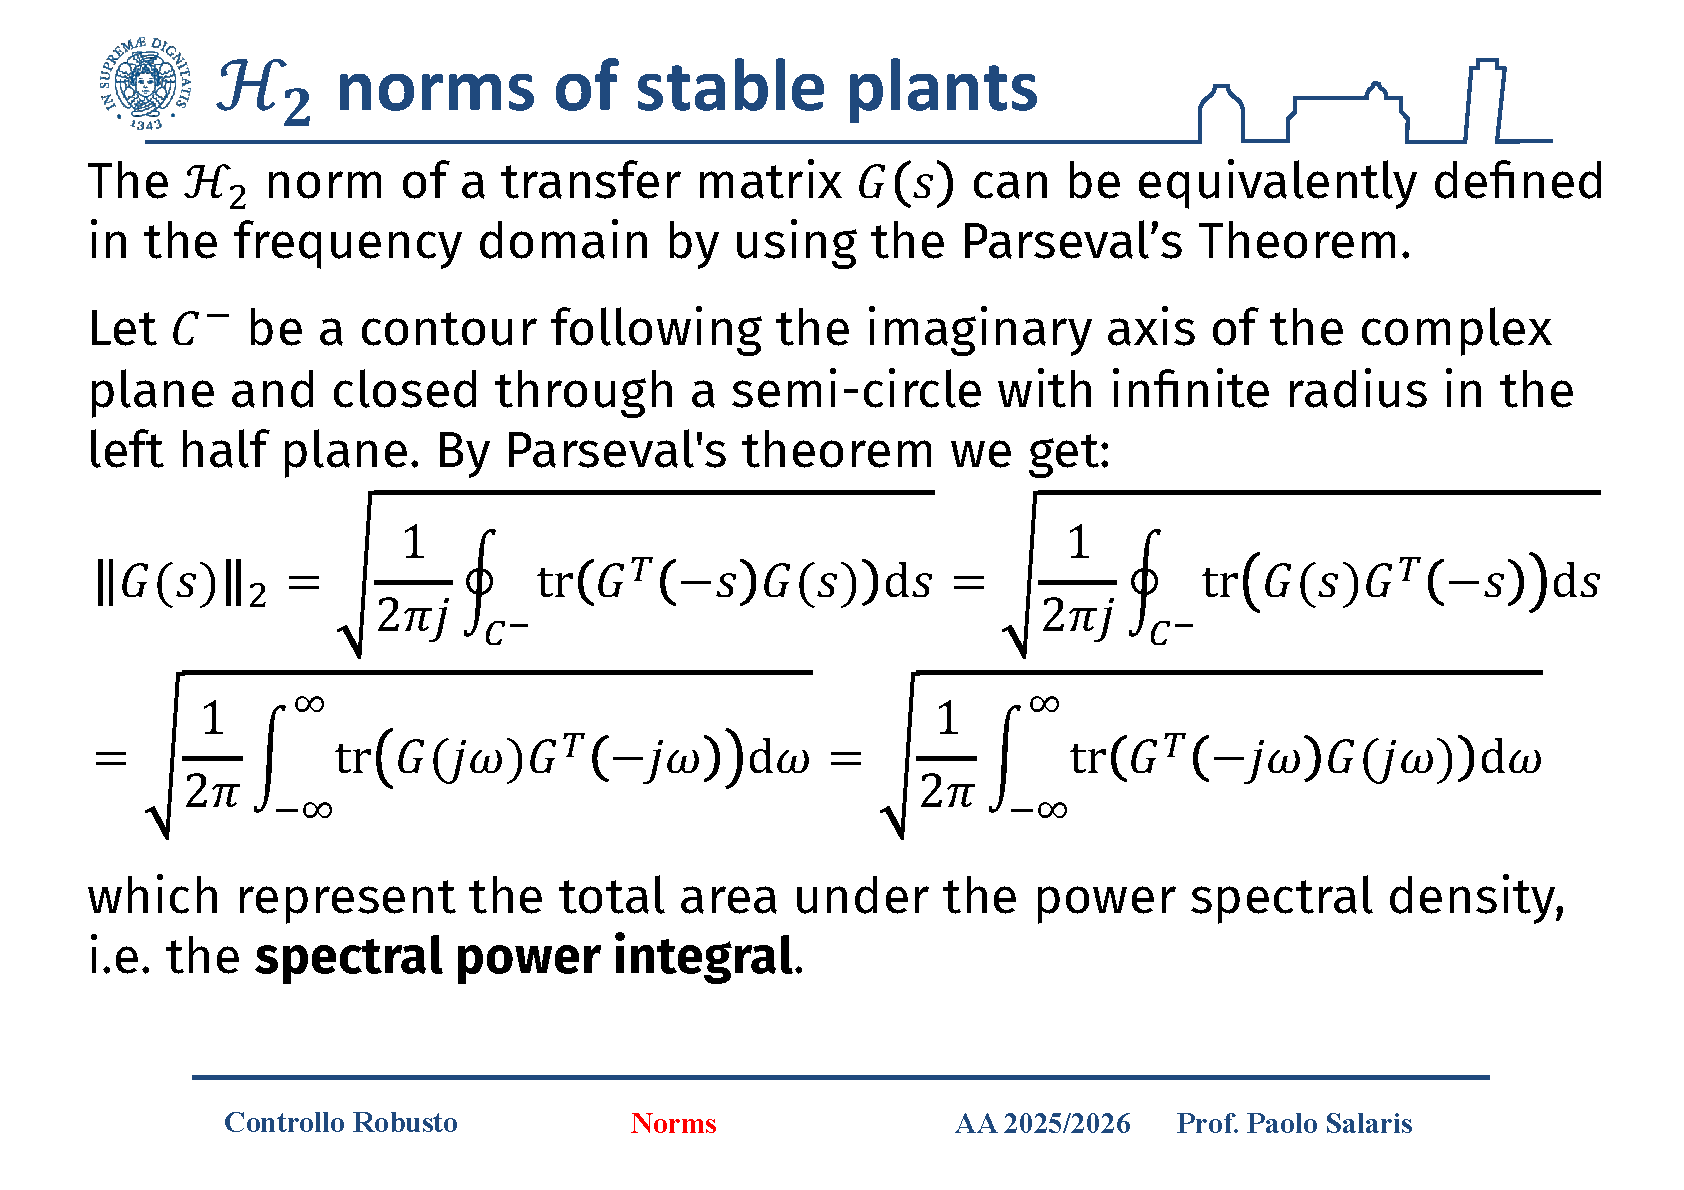
\includegraphics[width=\linewidth]{images6/norms-11-32-011.png}
        \caption{Passaggio da risposta impulsiva a integrale frequenziale tramite Parseval.}
    \end{subfigure}
    \hfill
    \begin{subfigure}{0.48\textwidth}
        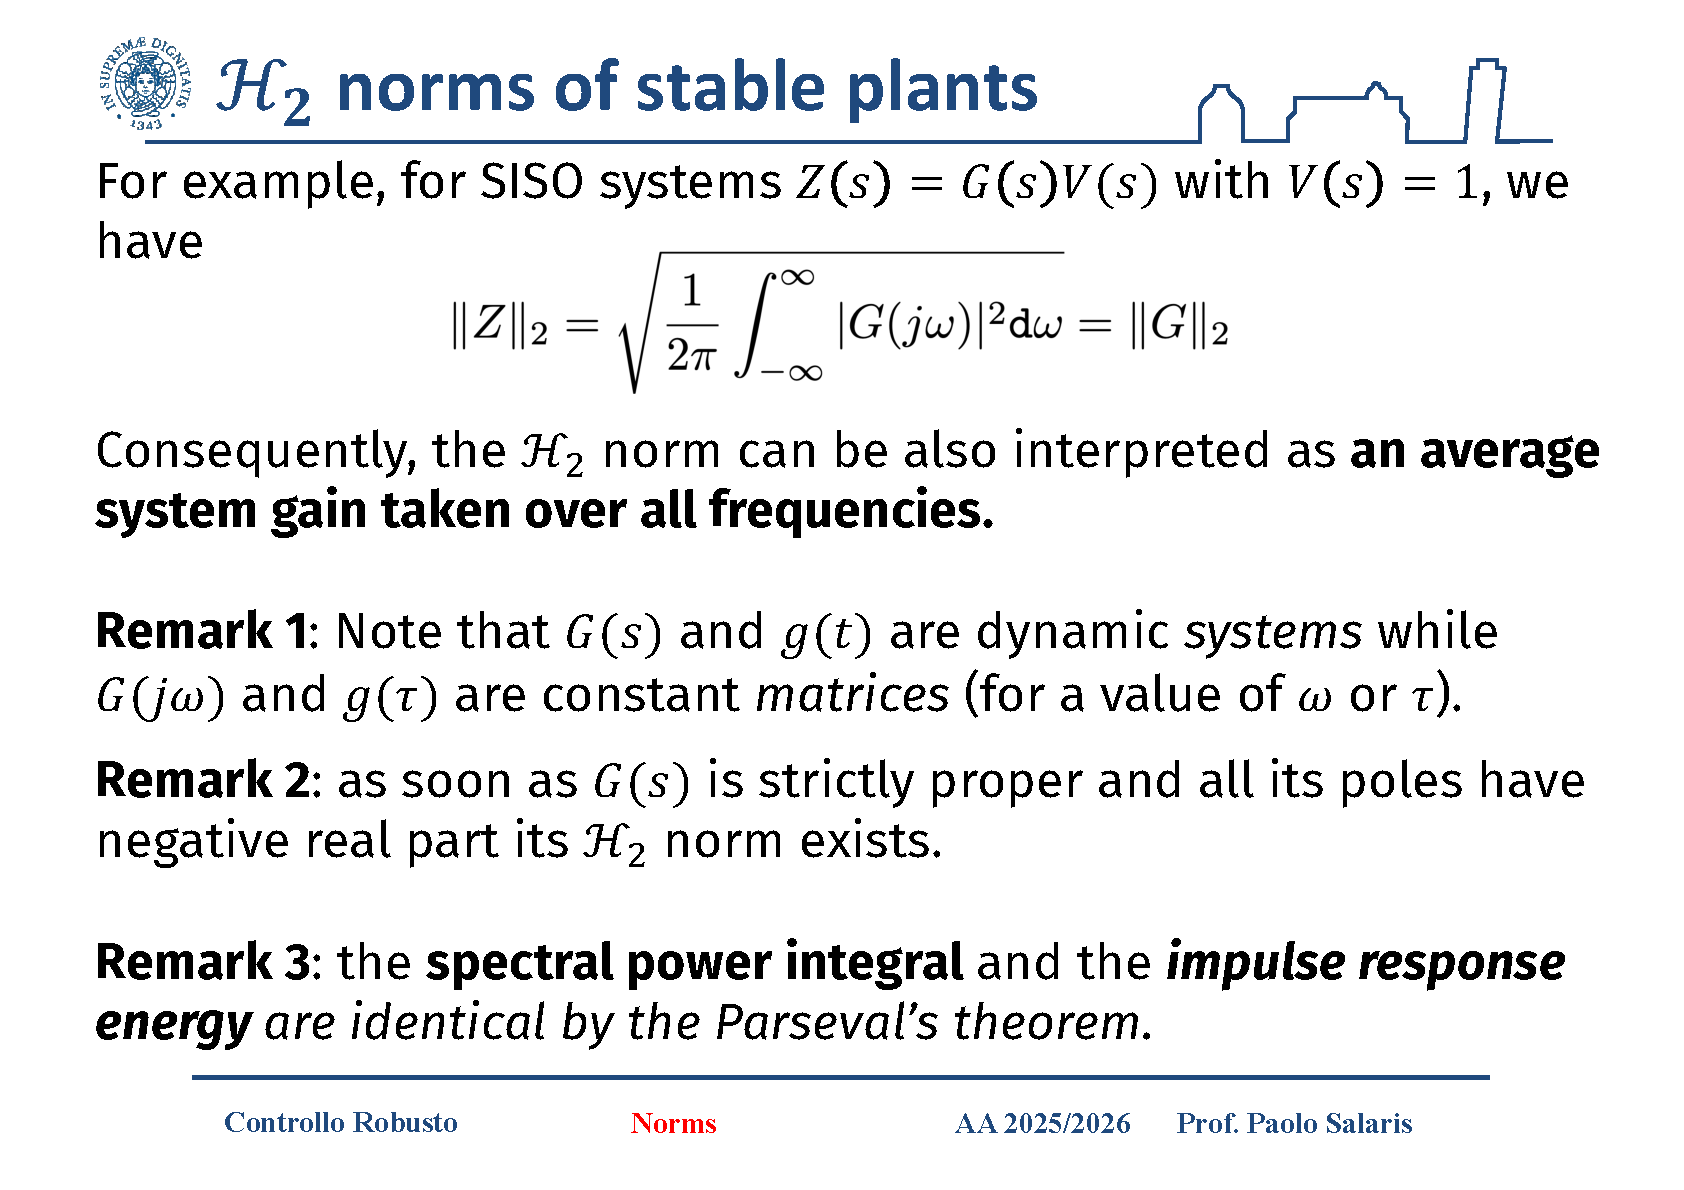
\includegraphics[width=\linewidth]{images6/norms-11-32-012.png}
        \caption{Interpretazione della norma $H_2$ come guadagno medio sulle frequenze.}
    \end{subfigure}
    \caption{Tempo e frequenza descrivono la stessa norma $H_2$ da due punti di vista complementari.}
\end{figure}

\subsubsection{Forma con norma di Frobenius e valori singolari}

Poich\'e
$$
\operatorname{tr}\!\bigl(G(-j\omega)^T G(j\omega)\bigr)=\|G(j\omega)\|_F^2,
$$
la norma $H_2$ si pu\`o riscrivere come
$$
\|G\|_{H_2}^2
=
\frac{1}{2\pi}\int_{-\infty}^{\infty}\|G(j\omega)\|_F^2\,d\omega.
$$
Usando poi la decomposizione in valori singolari si ottiene
$$
\|G\|_{H_2}^2
=
\frac{1}{2\pi}\sum_{k=1}^{q}\int_{-\infty}^{\infty}\sigma_k^2\!\bigl(G(j\omega)\bigr)\,d\omega,
\qquad q=\min\{p,m\}.
$$

Questa forma \`e particolarmente ricca dal punto di vista interpretativo. In ogni frequenza, i valori singolari descrivono come il sistema amplifica le diverse direzioni di ingresso. Integrare il quadrato di tutti i valori singolari significa quindi sommare, su tutte le frequenze e su tutte le direzioni principali, il contenuto energetico della risposta del sistema.

Si capisce cos\`\i\ anche perch\'e l'$H_2$ \`e una norma ``globale'': non guarda solo alla direzione peggiore, ma tiene conto dell'intero spettro direzionale del sistema. Per questo pu\`o essere molto adatta quando si vuole minimizzare una prestazione media o quadratica, mentre \`e meno adatta quando interessa solo il caso peggiore.

\begin{figure}[H]
    \centering
    \begin{subfigure}{0.48\textwidth}
        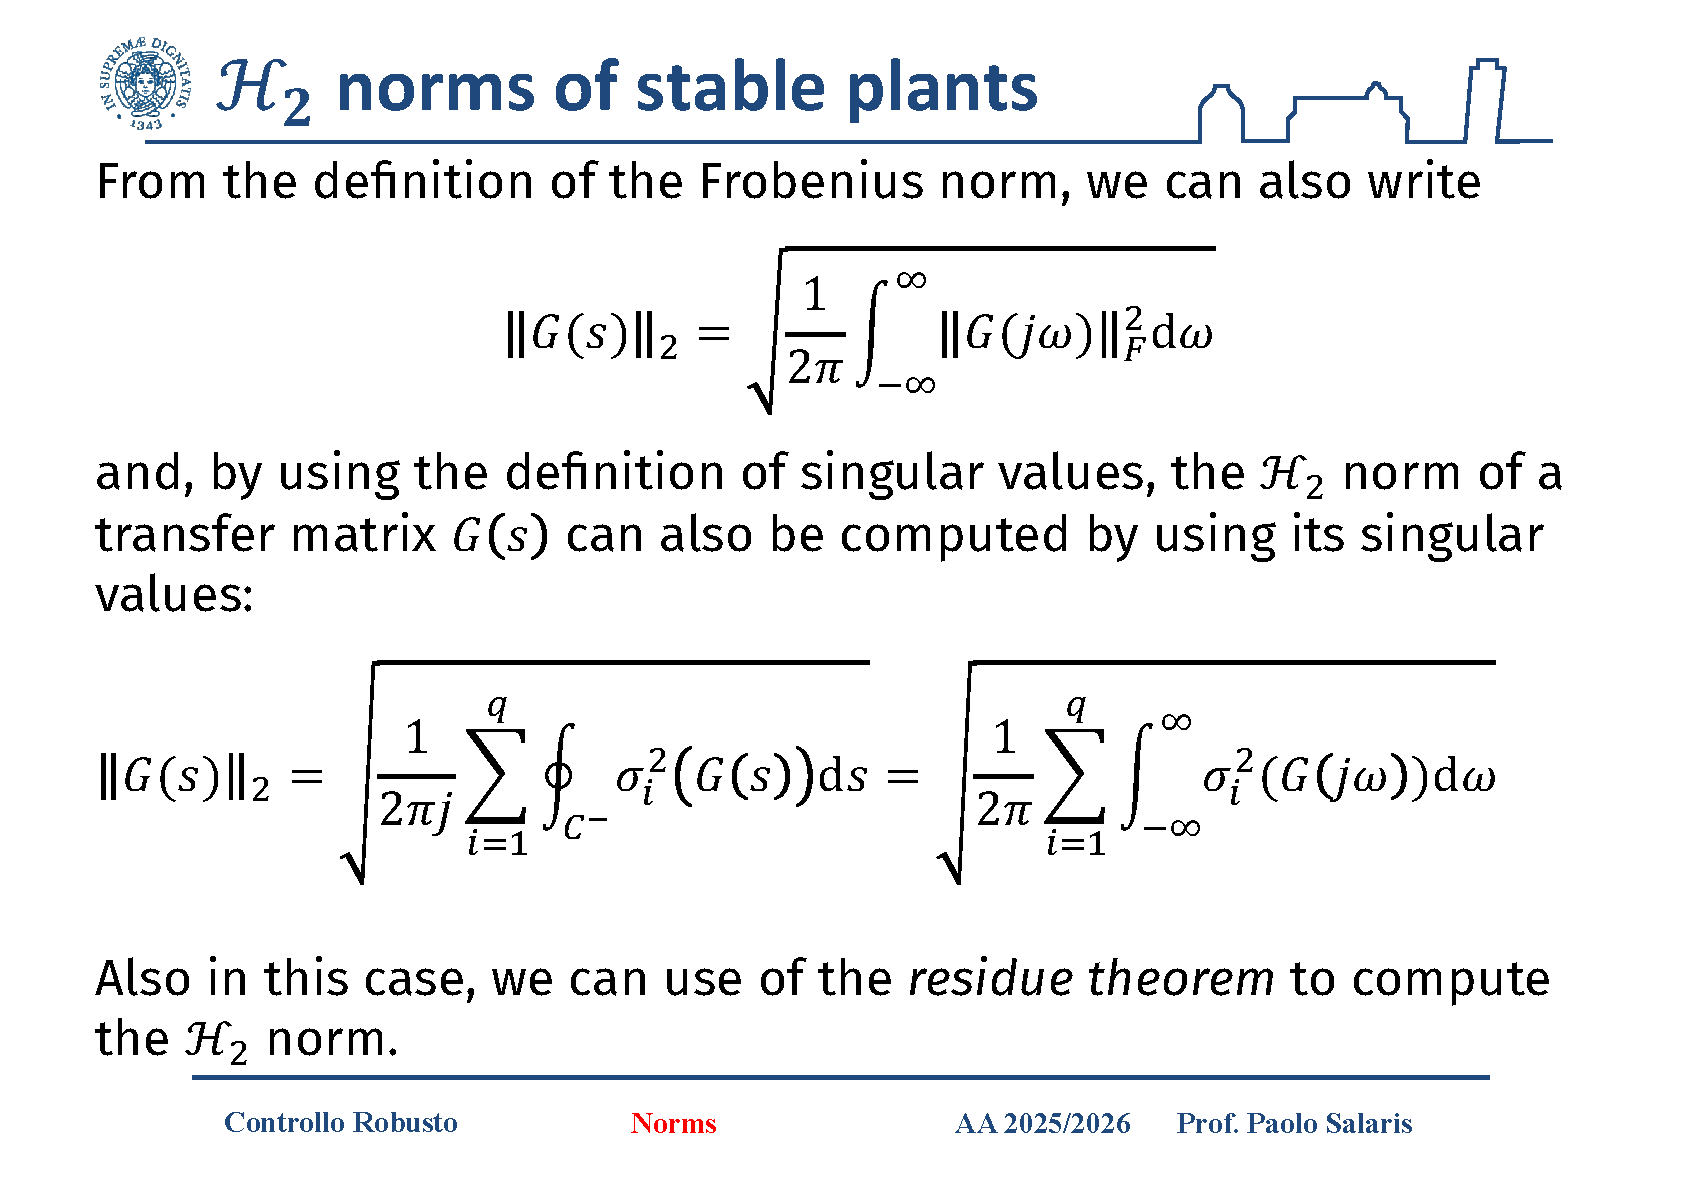
\includegraphics[width=\linewidth]{images6/norms-11-32-013.png}
        \caption{Riformulazione della norma $H_2$ tramite norma di Frobenius e valori singolari.}
    \end{subfigure}
    \hfill
    \begin{subfigure}{0.48\textwidth}
        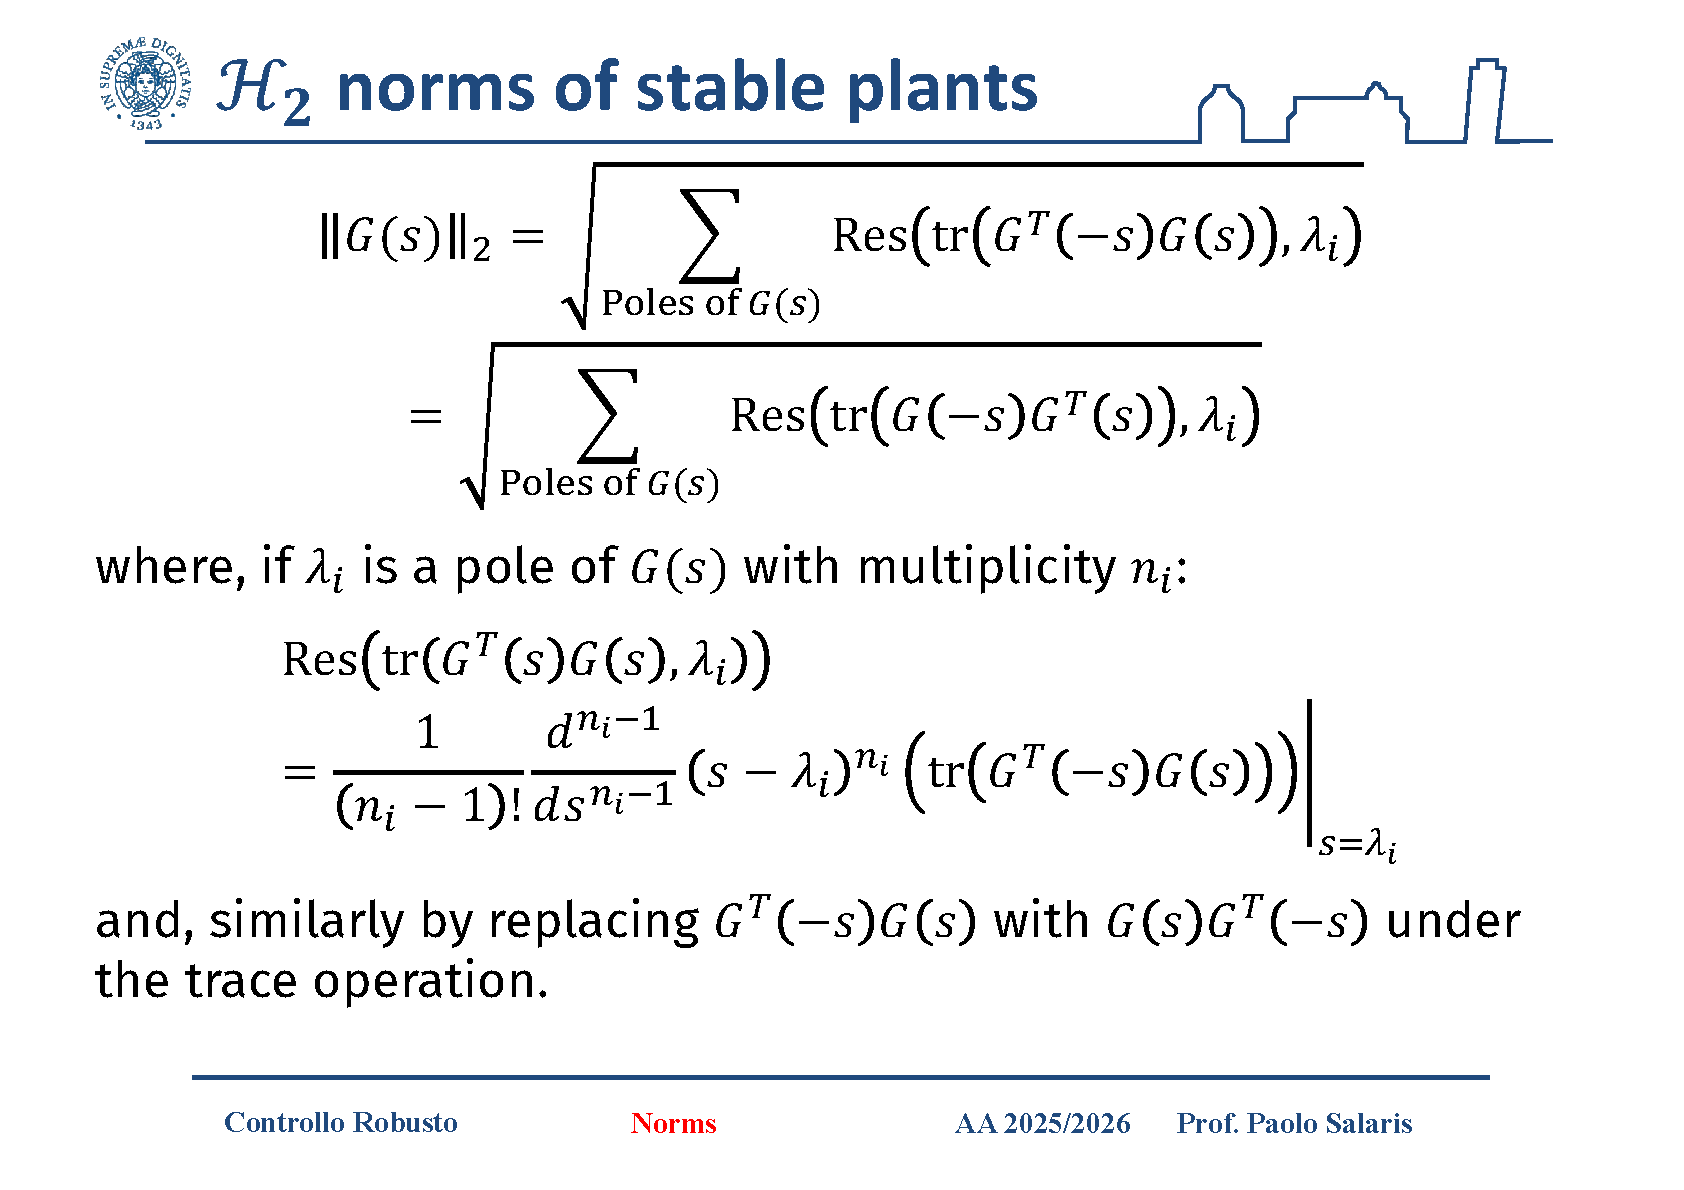
\includegraphics[width=\linewidth]{images6/norms-11-32-014.png}
        \caption{Formula tramite teorema dei residui per il calcolo della norma $H_2$.}
    \end{subfigure}
    \caption{Le forme con Frobenius, valori singolari e residui sono tre strumenti equivalenti ma utili in contesti diversi.}
\end{figure}

\subsubsection{Calcolo mediante residui}

Come per la norma $L_2$ dei segnali, anche la norma $H_2$ pu\`o essere calcolata senza integrare esplicitamente lungo tutte le frequenze. Se $G(s)$ \`e stabile e strettamente propria, allora
$$
\|G\|_{H_2}^2
=
\sum_{\lambda_i\in\mathrm{poli}(G)}
\operatorname{Res}\!\Bigl(\operatorname{tr}\!\bigl(G^T(-s)G(s)\bigr),\lambda_i\Bigr),
$$
dove la somma va fatta sui poli stabili di $G$. Per poli semplici la formula del residuo \`e immediata; per poli multipli si usa la derivata di ordine opportuno riportata in slide.

Dal punto di vista operativo, questa formula \`e preziosa perch\'e sostituisce un integrale frequenziale infinito con una somma finita di contributi locali associati ai poli. Dal punto di vista concettuale, invece, mette in luce che la norma $H_2$ \`e profondamente legata alla struttura modale del sistema: i modi lenti, i modi poco smorzati e i modi molto eccitabili contribuiscono in modo diretto al suo valore complessivo.

\subsection{Interpretazione stocastica della norma \texorpdfstring{$H_2$}{H2}}

Le slide successive propongono una delle interpretazioni pi\`u belle dell'$H_2$. Se l'ingresso $u(t)$ \`e un rumore bianco a media nulla e covarianza unitaria,
$$
\mathbb{E}[u(t)] = 0,
\qquad
\mathbb{E}[u(t)u(t-\tau)] = \delta(\tau)I,
$$
allora il quadrato della norma $H_2$ coincide con la varianza a regime dell'uscita.

Nel caso SISO, se
$$
z(t)=\int_0^\infty g(\tau)\,u(t-\tau)\,d\tau,
$$
allora
$$
\mathbb{E}[z^2(t)]
=
\int_0^\infty\int_0^\infty
g(\tau_1)g(\tau_2)\,
\mathbb{E}[u(t-\tau_1)u(t-\tau_2)]\,
d\tau_1\,d\tau_2.
$$
Sfruttando la propriet\`a del rumore bianco,
$$
\mathbb{E}[u(t-\tau_1)u(t-\tau_2)] = \delta(\tau_1-\tau_2),
$$
il doppio integrale collassa in
$$
\mathbb{E}[z^2(t)]
=
\int_0^\infty g^2(\tau)\,d\tau
=
\|G\|_{H_2}^2.
$$

Questa relazione \`e estremamente significativa. Dice che una piccola norma $H_2$ equivale a una piccola varianza di uscita quando il sistema \`e eccitato da disturbi casuali ``piatti'' in frequenza. In altre parole, l'$H_2$ \`e la misura naturale di prestazione quando il modello del disturbo \`e stocastico e si vuole minimizzare l'energia media trasmessa all'uscita.

\begin{figure}[H]
    \centering
    \begin{subfigure}{0.48\textwidth}
        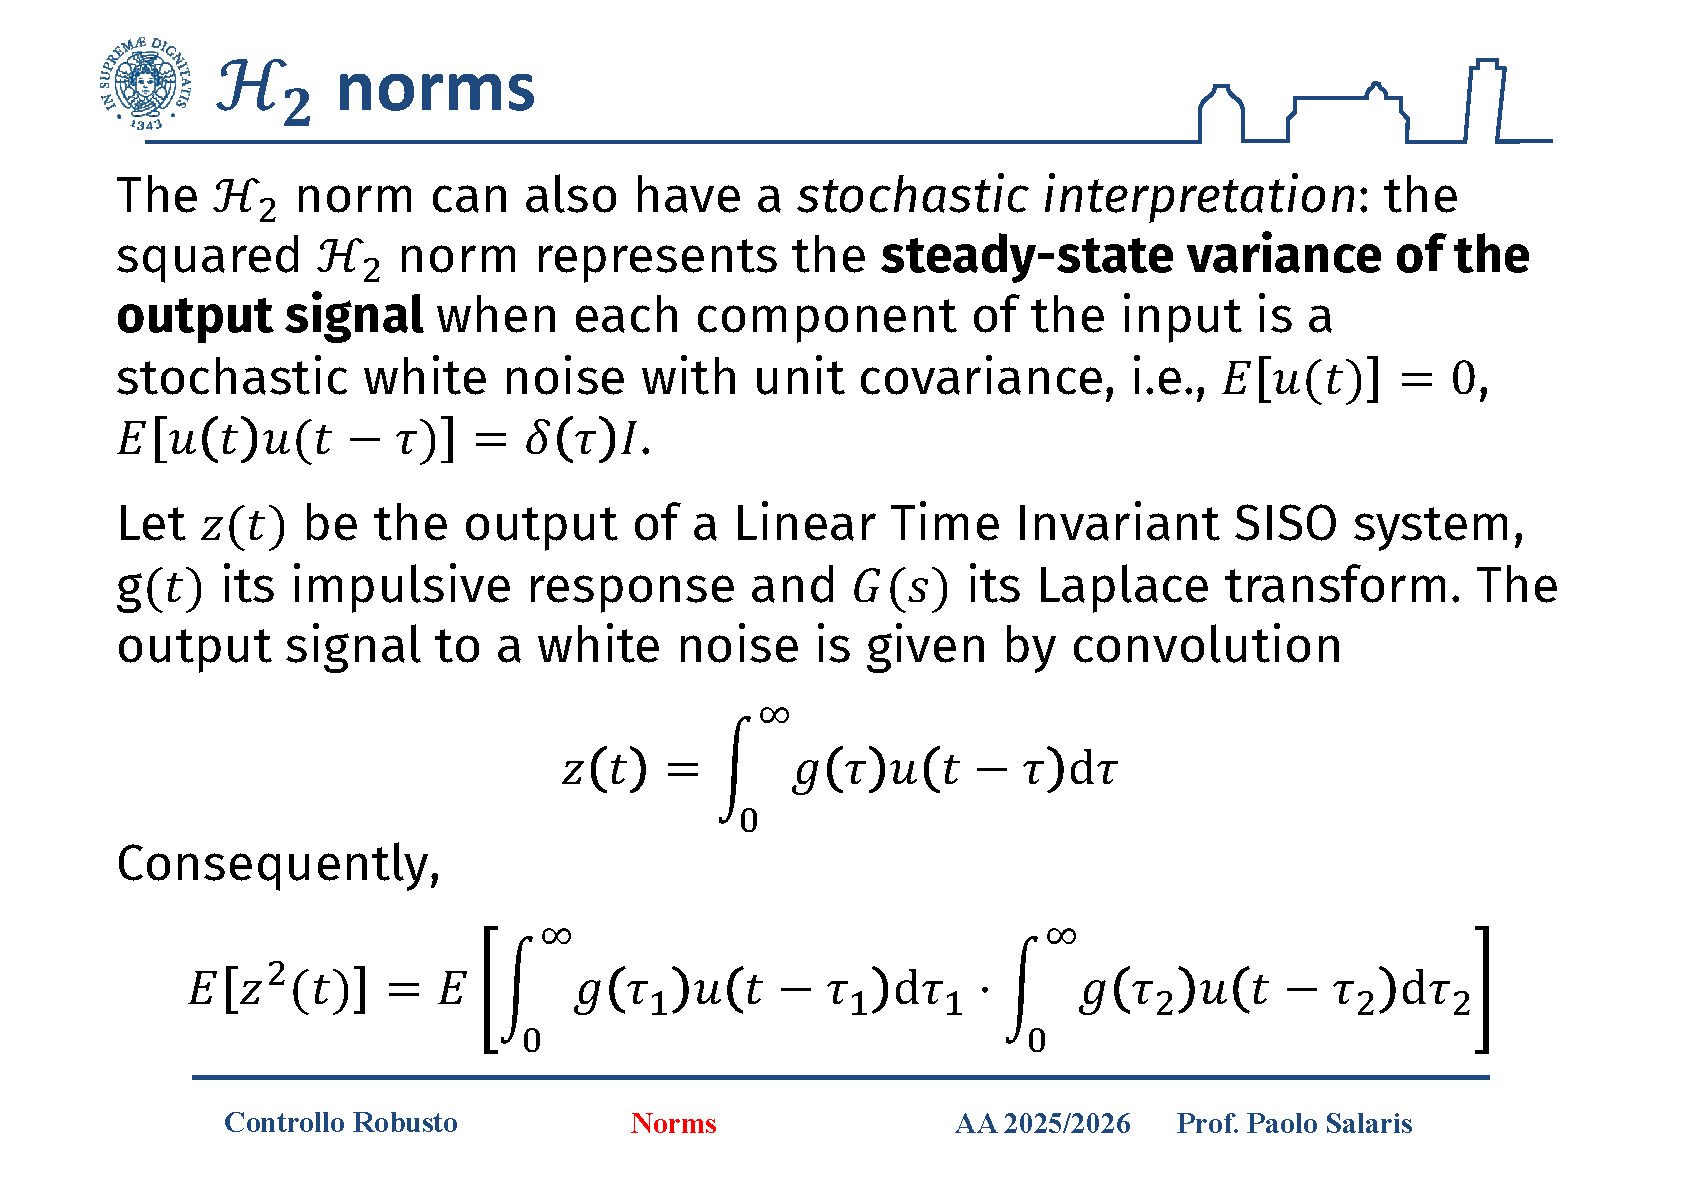
\includegraphics[width=\linewidth]{images6/norms-11-32-015.png}
        \caption{Impostazione del problema con ingresso di rumore bianco e uscita ottenuta per convoluzione.}
    \end{subfigure}
    \hfill
    \begin{subfigure}{0.48\textwidth}
        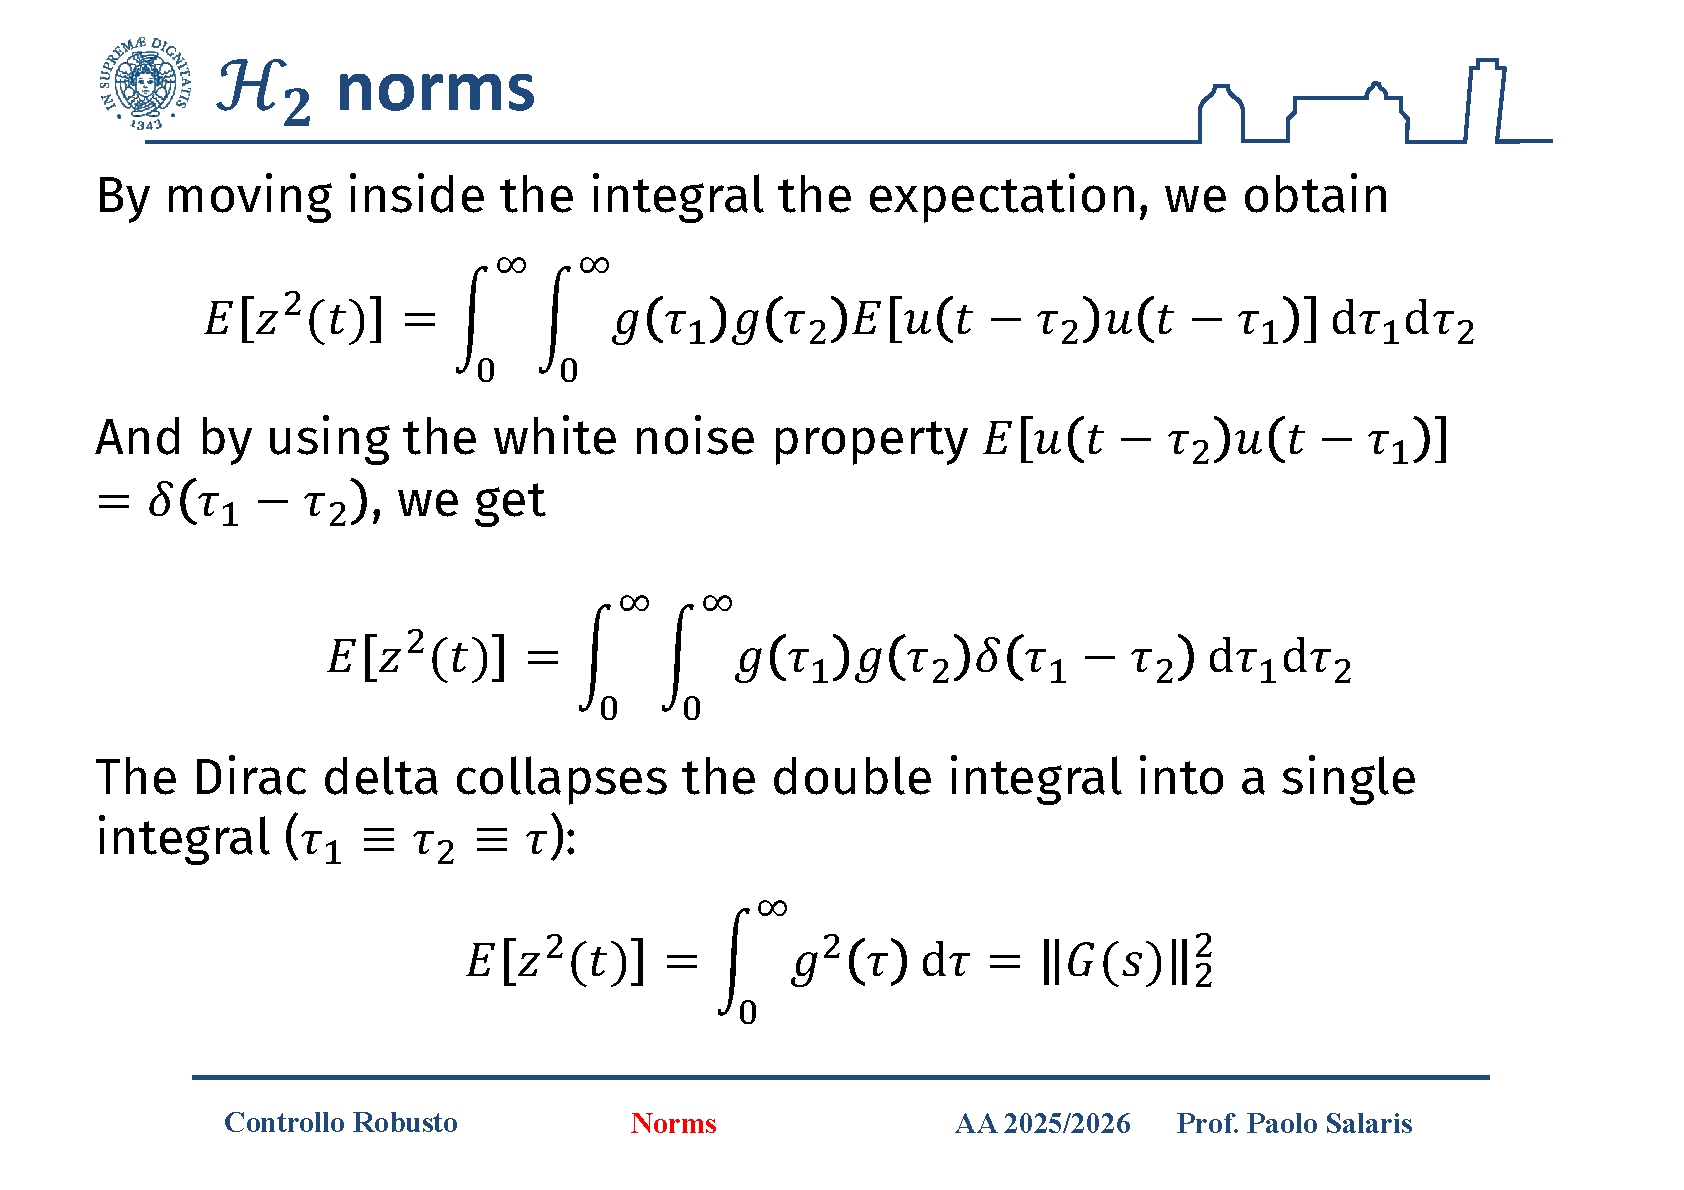
\includegraphics[width=\linewidth]{images6/norms-11-32-016.png}
        \caption{Uso della delta di Dirac per ricondurre la varianza all'energia della risposta impulsiva.}
    \end{subfigure}
    \caption{L'interpretazione stocastica collega l'$H_2$ alla prestazione media del sistema in presenza di rumore bianco.}
\end{figure}

La slide riassuntiva finale di questo blocco mostra in modo molto efficace le tre ``facce'' della norma $H_2$:
\begin{itemize}
    \item \textbf{faccia temporale:} energia della risposta impulsiva;
    \item \textbf{faccia frequenziale:} area totale della potenza spettrale;
    \item \textbf{faccia stocastica:} varianza dell'uscita a regime per ingresso di rumore bianco unitario.
\end{itemize}

Queste tre letture non sono tre definizioni diverse, ma tre modi equivalenti di guardare alla stessa quantit\`a. Questa equivalenza \`e una delle ragioni per cui la norma $H_2$ occupa un posto cos\`\i\ centrale nell'analisi e nella sintesi dei controlli robusti.

\begin{figure}[H]
    \centering
    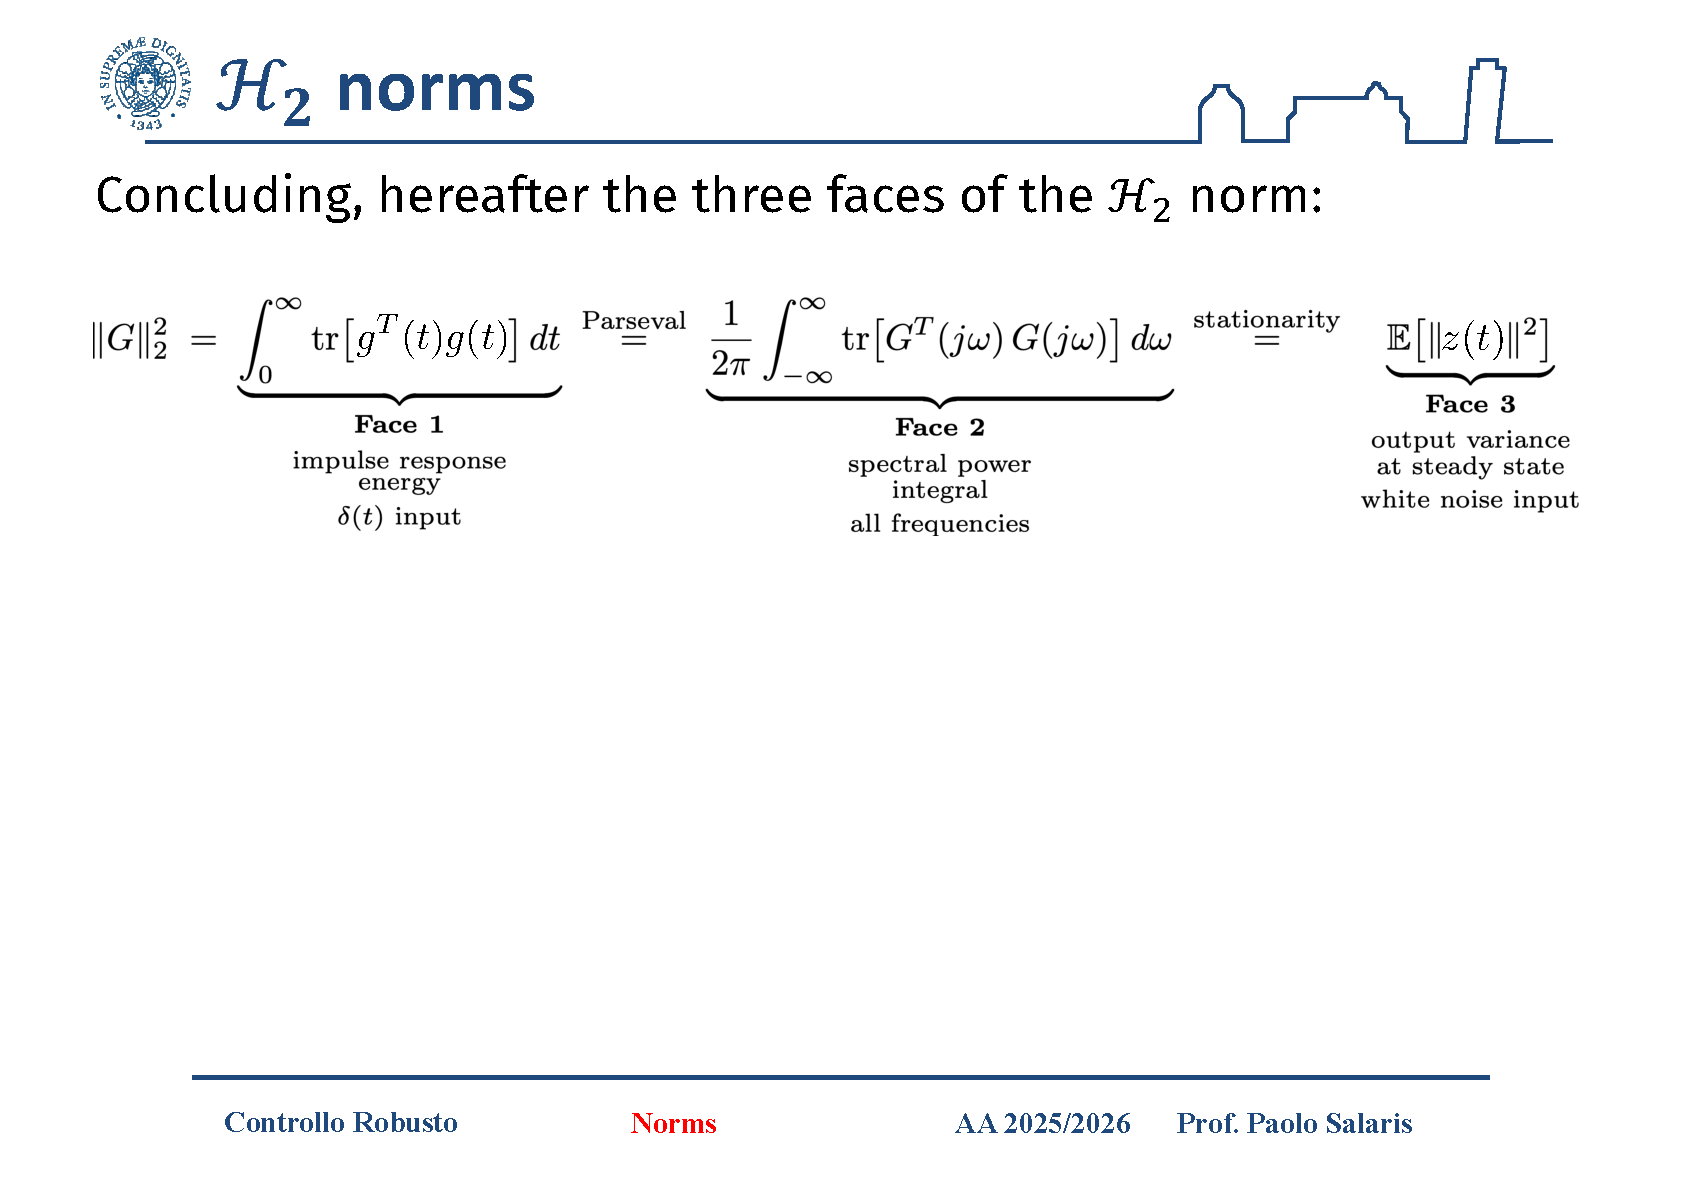
\includegraphics[width=0.82\textwidth]{images6/norms-11-32-017.png}
    \caption{La norma $H_2$ unifica energia della risposta impulsiva, potenza spettrale e varianza di uscita a regime.}
\end{figure}

\subsection{Esempio: norma \texorpdfstring{$H_2$}{H2} di un sistema del secondo ordine}

Le ultime cinque slide della lezione applicano il teorema dei residui a un esempio molto classico:
$$
\ddot y(t)+2\xi\omega_n\dot y(t)+\omega_n^2 y(t)=K\omega_n^2 u(t),
$$
dove $\xi>0$ \`e il coefficiente di smorzamento, $\omega_n>0$ la pulsazione naturale e $K$ il guadagno statico. Assumendo $0<\xi<1$, i poli sono complessi coniugati:
$$
\lambda_1=-\xi\omega_n+j\omega_n\sqrt{1-\xi^2},
\qquad
\lambda_2=-\xi\omega_n-j\omega_n\sqrt{1-\xi^2}.
$$
La funzione di trasferimento risulta quindi
$$
F(s)=\frac{K\omega_n^2}{(s-\lambda_1)(s-\lambda_2)}.
$$

Le slide scelgono di non passare dalla risposta impulsiva esplicita, ma di sfruttare direttamente la formula ai residui:
$$
\|F\|_{H_2}^2
=
\operatorname{Res}\!\bigl(F(-s)F(s),\lambda_1\bigr)
+
\operatorname{Res}\!\bigl(F(-s)F(s),\lambda_2\bigr).
$$
Poich\'e i poli sono semplici, i residui si calcolano in modo diretto. Inoltre, dato che $\lambda_2=\overline{\lambda_1}$, i due contributi sono complessi coniugati e la loro somma \`e due volte la parte reale del primo. Questo semplifica molto l'algebra e porta al risultato finale
$$
\|F\|_{H_2}^2=\frac{K^2\omega_n}{4\xi},
\qquad
\|F\|_{H_2}=|K|\sqrt{\frac{\omega_n}{4\xi}}.
$$

La slide finale scrive il risultato con $K$ al posto di $|K|$, sottintendendo il caso usuale $K>0$. Nel testo conviene invece esplicitare il valore assoluto, perch\'e una norma deve sempre essere non negativa.

Questo esempio \`e molto istruttivo anche dal punto di vista fisico. Dice infatti che:
\begin{itemize}
    \item aumentando $\omega_n$ cresce la norma $H_2$, quindi il sistema diventa pi\`u ``energetico'' nella sua risposta impulsiva;
    \item aumentando lo smorzamento $\xi$ la norma diminuisce, cio\`e il sistema disperde meglio l'energia e amplifica meno il rumore bianco;
    \item il guadagno statico $K$ entra linearmente nella norma, come era ragionevole aspettarsi.
\end{itemize}
In altre parole, la norma $H_2$ traduce in una formula compatta intuizioni fisiche molto concrete su rapidit\`a, smorzamento e amplificazione.

\begin{figure}[H]
    \centering
    \begin{subfigure}{0.48\textwidth}
        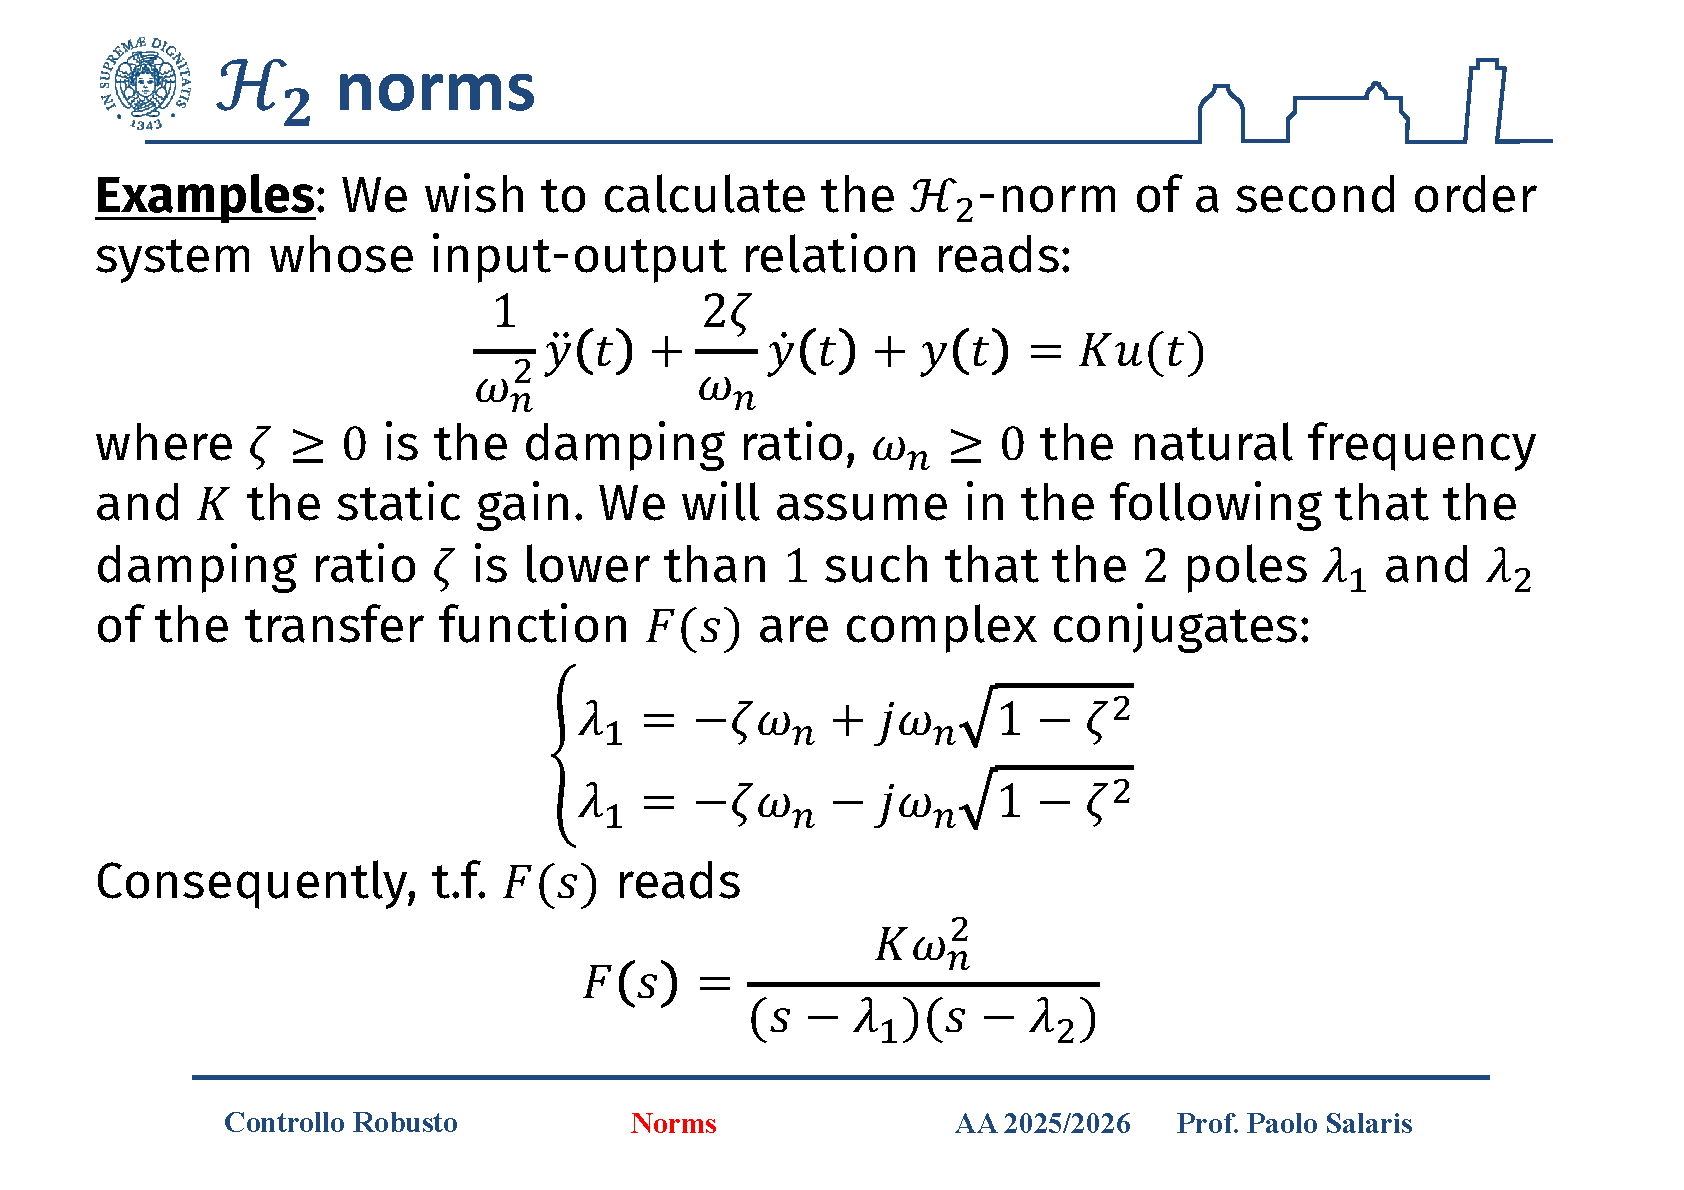
\includegraphics[width=\linewidth]{images6/norms-11-32-018.png}
        \caption{Definizione del sistema del secondo ordine e posizione dei poli complessi coniugati.}
    \end{subfigure}
    \hfill
    \begin{subfigure}{0.48\textwidth}
        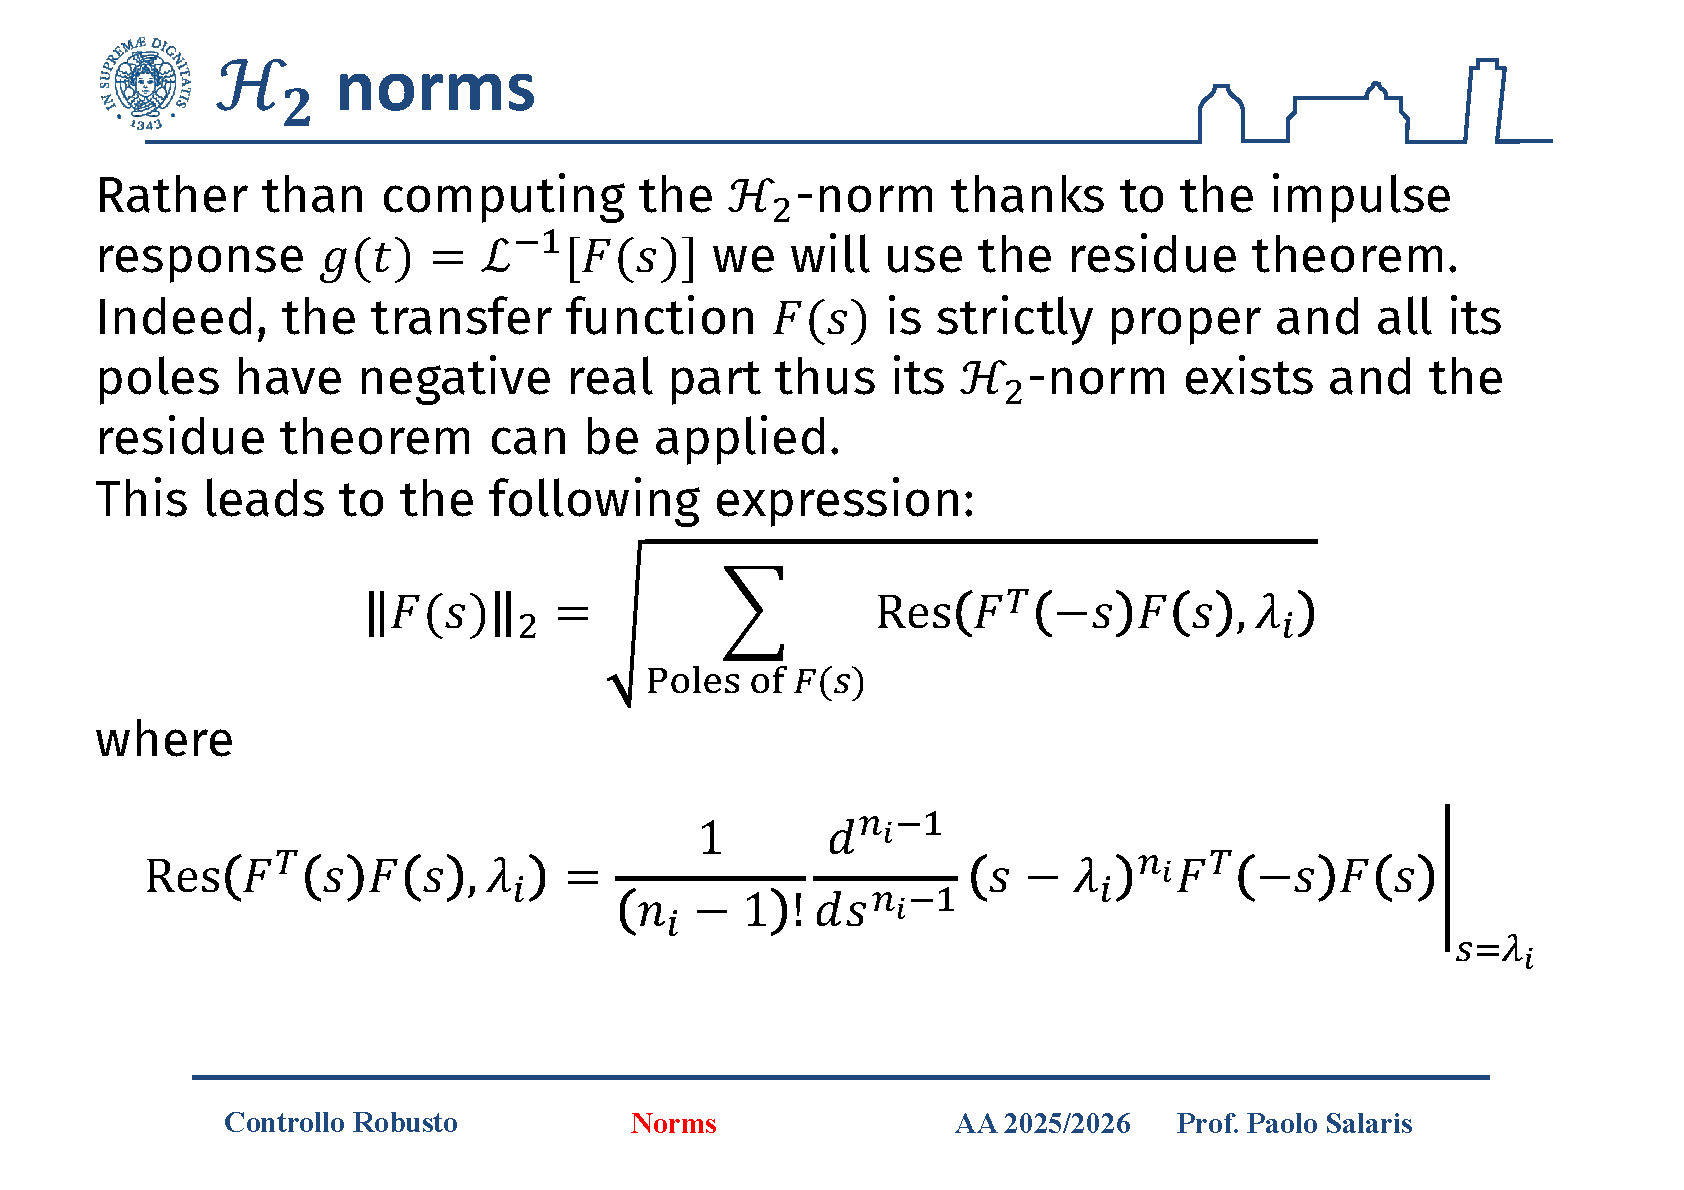
\includegraphics[width=\linewidth]{images6/norms-11-32-019.png}
        \caption{Impostazione del calcolo della norma $H_2$ tramite teorema dei residui.}
    \end{subfigure}
    \caption{L'esempio mostra come la formula generale dell'$H_2$ si traduca in un calcolo esplicito sui poli del sistema.}
\end{figure}

\begin{figure}[H]
    \centering
    \begin{subfigure}{0.48\textwidth}
        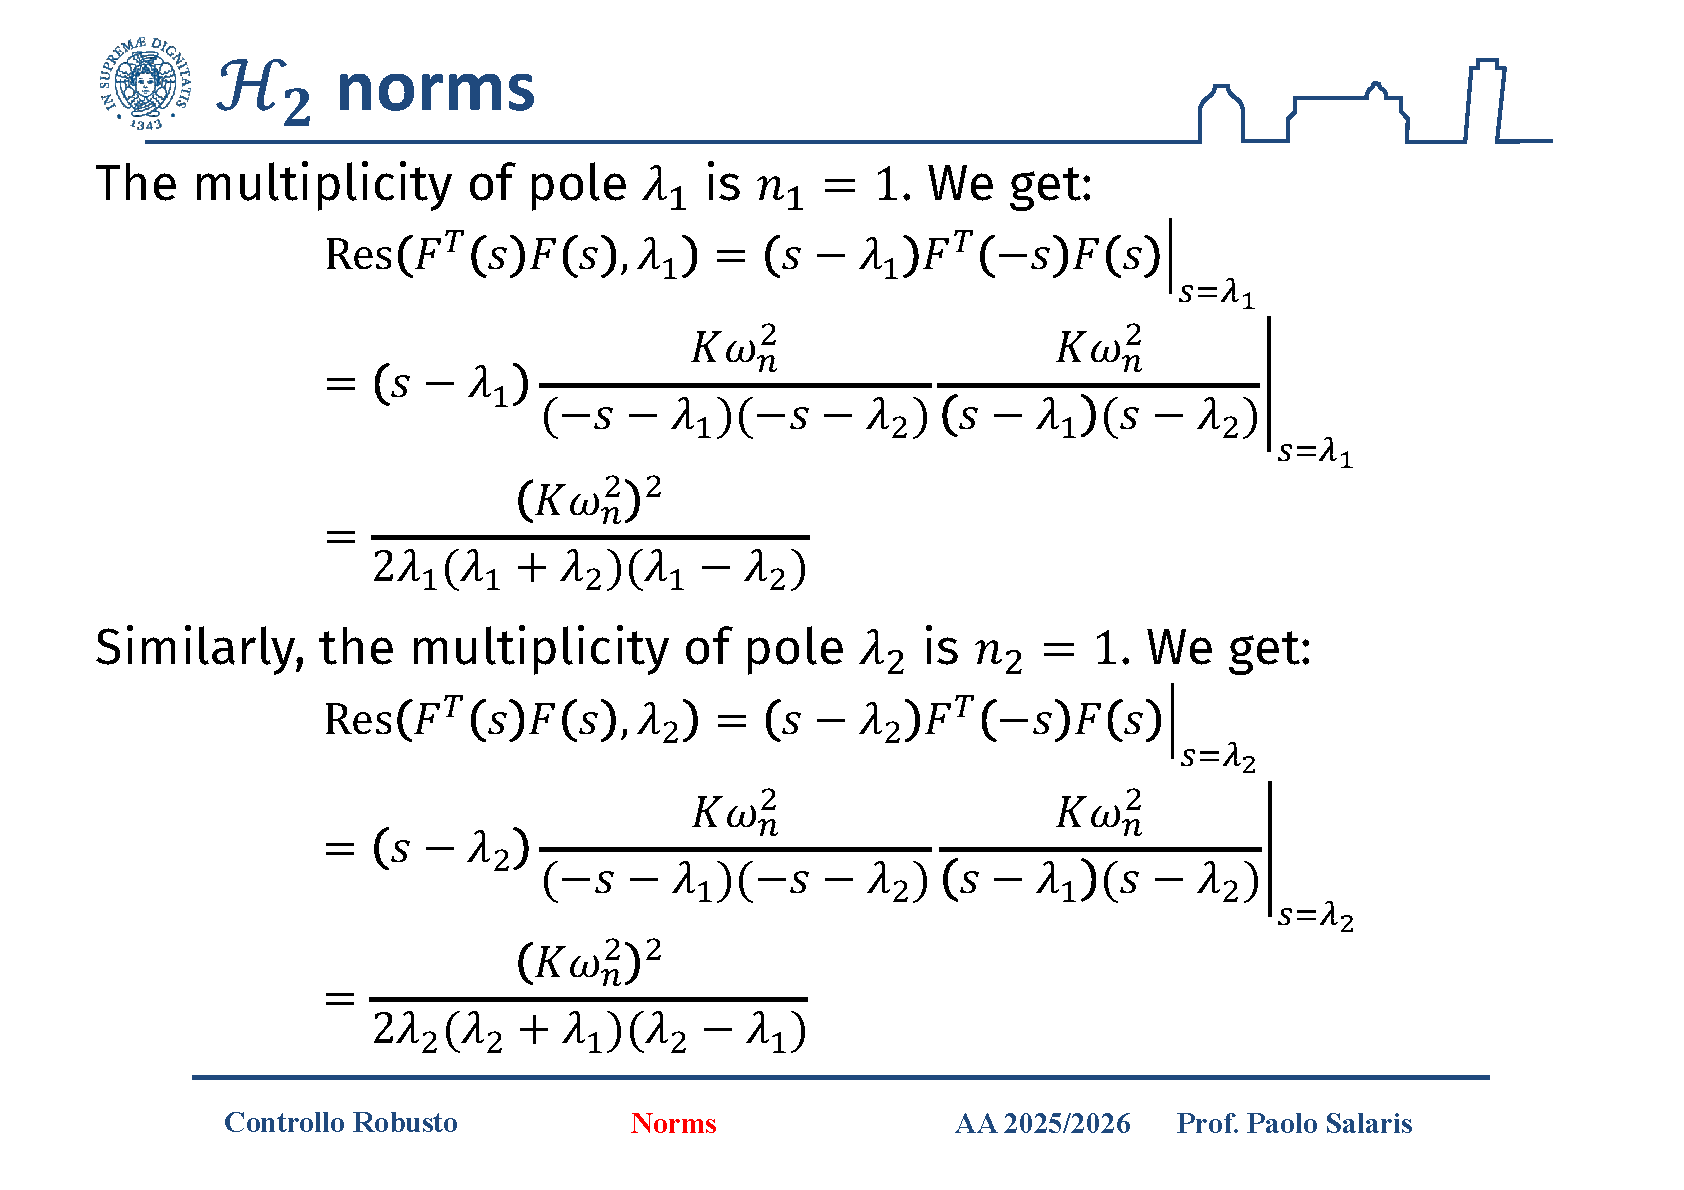
\includegraphics[width=\linewidth]{images6/norms-11-32-020.png}
        \caption{Calcolo dei residui associati ai due poli semplici del trasferimento.}
    \end{subfigure}
    \hfill
    \begin{subfigure}{0.48\textwidth}
        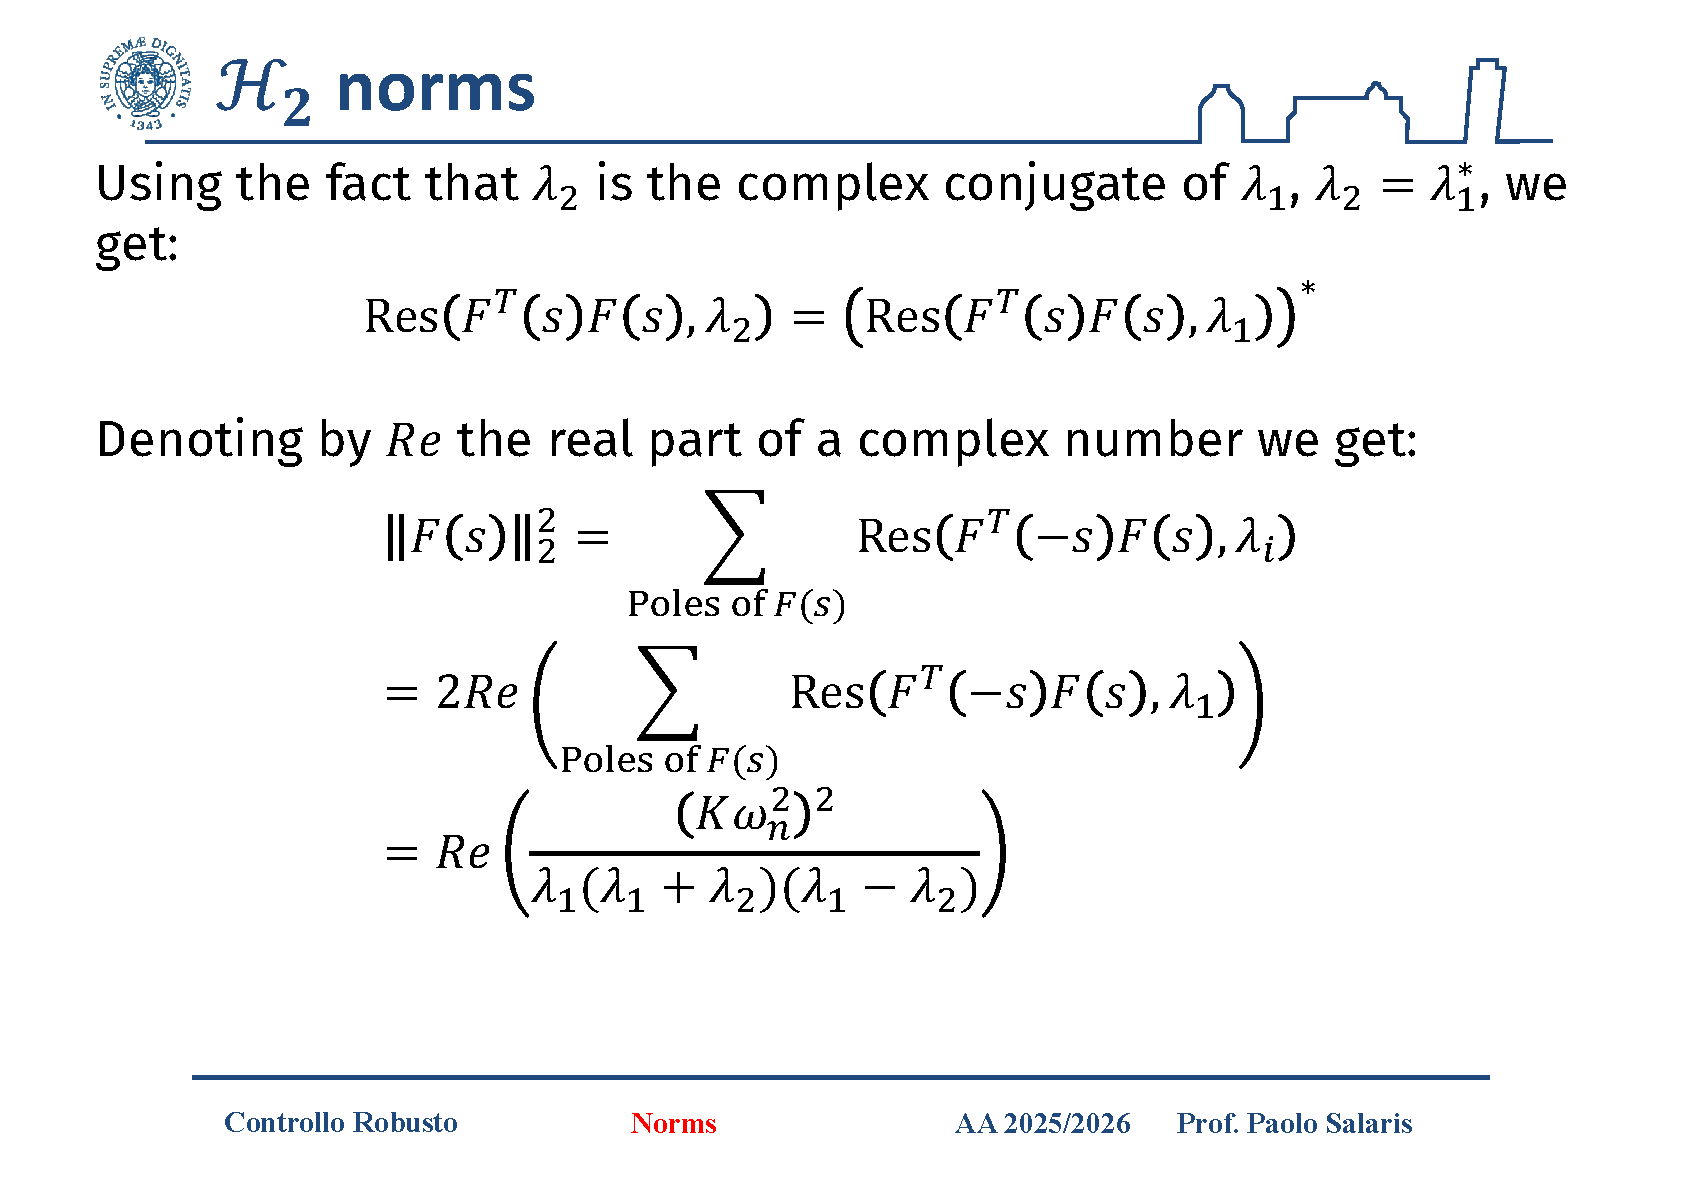
\includegraphics[width=\linewidth]{images6/norms-11-32-021.png}
        \caption{Uso della simmetria complessa per sommare i due contributi in forma compatta.}
    \end{subfigure}
    \caption{Il fatto che i poli siano complessi coniugati rende l'algebra pi\`u semplice e mostra il ruolo della parte reale.}
\end{figure}

\begin{figure}[H]
    \centering
    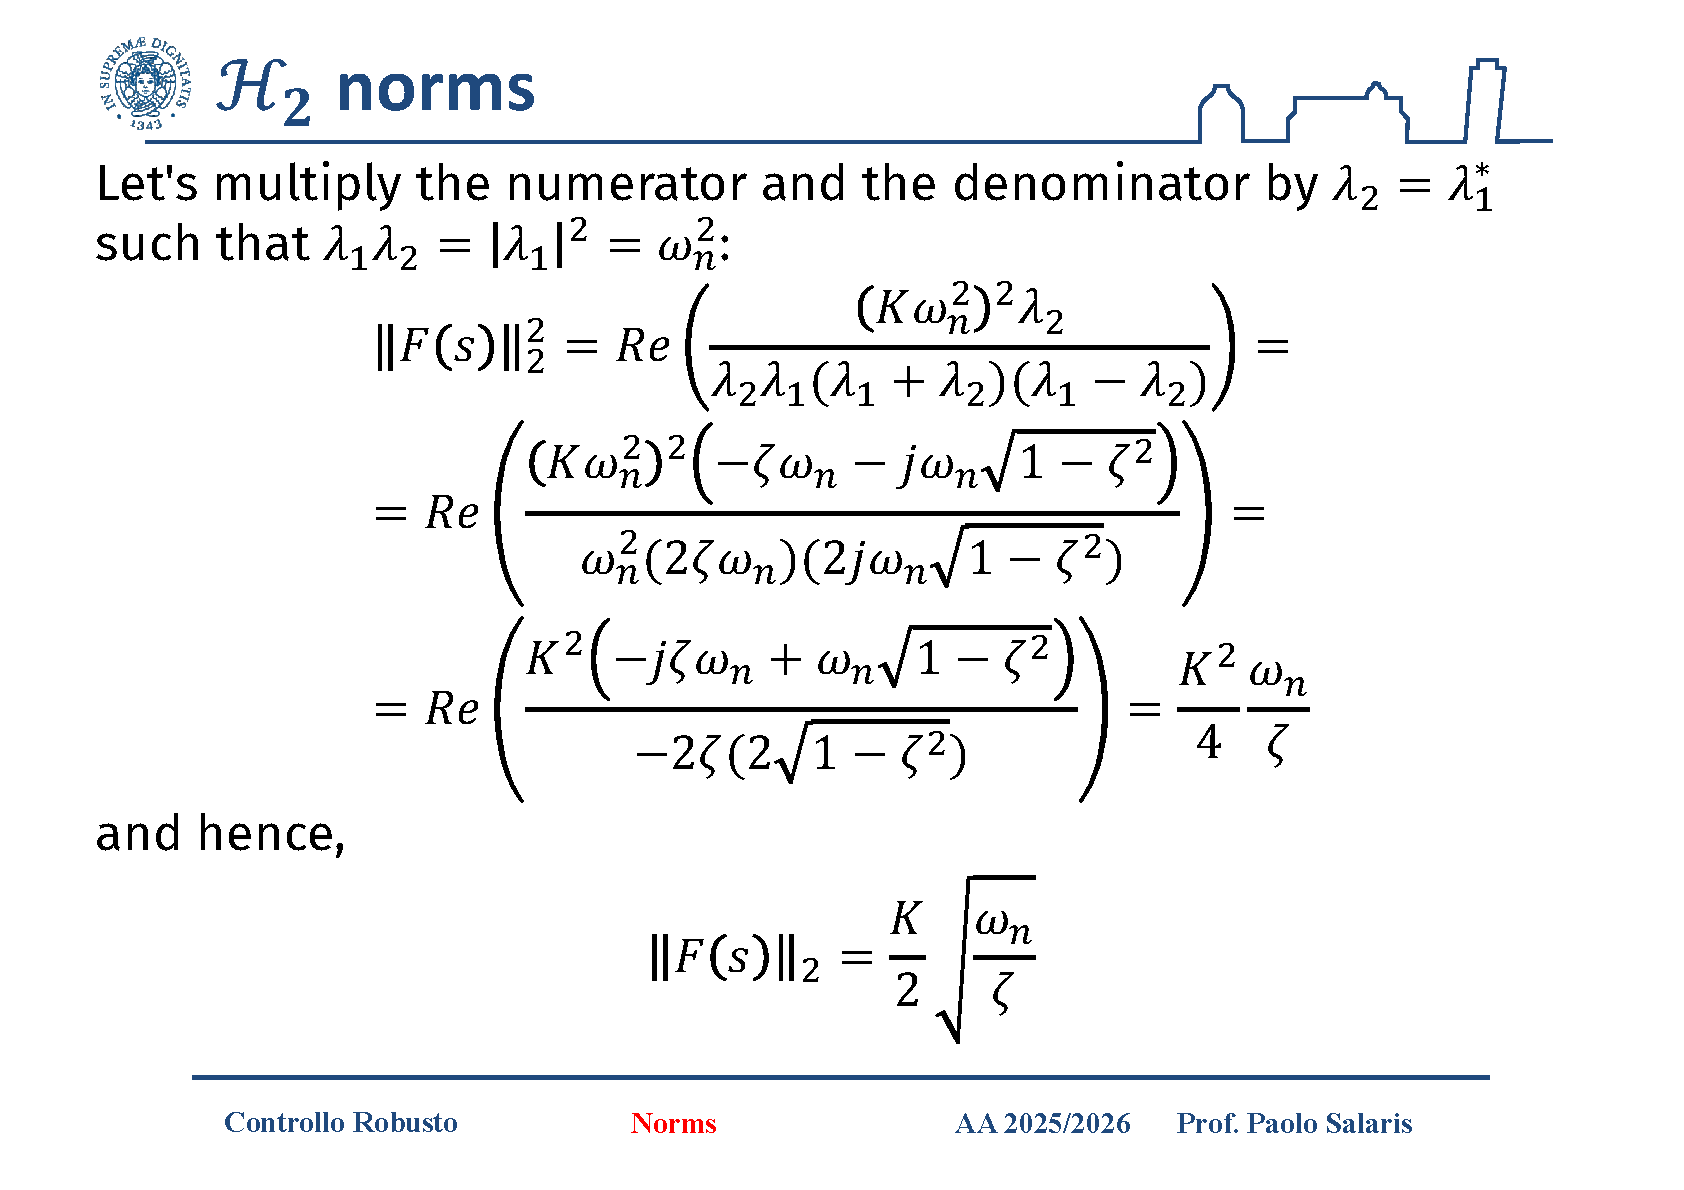
\includegraphics[width=0.68\textwidth]{images6/norms-11-32-022.png}
    \caption{Risultato finale: la norma $H_2$ del secondo ordine cresce con $\omega_n$ e decresce con lo smorzamento $\xi$.}
\end{figure}

\subsection{Sintesi conclusiva della lezione}

La Lezione 7 completa il passaggio dalle norme dei segnali alle norme dei sistemi. Dopo aver chiarito che le norme $L_p$ e $L_\infty$ misurano aspetti diversi della grandezza di un segnale, la lezione mostra come la stessa idea possa essere trasferita a un sistema dinamico: non si misura pi\`u un segnale isolato, ma la capacit\`a del sistema di amplificare una classe di ingressi ammessi.

All'interno di questo quadro, la norma $H_2$ emerge come la misura naturale della risposta energetica di un sistema stabile e strettamente proprio. La sua forza sta nel fatto che unifica tre mondi diversi ma complementari: il dominio del tempo, il dominio della frequenza e l'interpretazione probabilistica. Per questo non \`e solo una quantit\`a da calcolare, ma una lente concettuale attraverso cui leggere il comportamento dinamico del sistema.

Sul piano operativo, la lezione lascia in mano quattro strumenti importanti:
\begin{itemize}
    \item la generalizzazione da $L_2$ alle norme $L_p$ e $L_\infty$ per segnali;
    \item la definizione della norma $H_2$ come energia della risposta impulsiva;
    \item la riformulazione della stessa norma tramite Parseval, Frobenius, valori singolari e residui;
    \item l'interpretazione dell'$H_2$ come varianza di uscita per ingresso di rumore bianco.
\end{itemize}
Questi strumenti preparano il terreno alle lezioni successive, in cui la norma $H_\infty$ e le specifiche robuste in termini di guadagni indotti verranno lette in modo sempre pi\`u sistematico.

\clearpage
\phantomsection
\section*{Appendice}
\addcontentsline{toc}{section}{Appendice}

\subsection*{Nota sulle convenzioni di \texorpdfstring{$H_2$}{H2}}
\phantomsection
\addcontentsline{toc}{subsection}{Nota sulle convenzioni di \texorpdfstring{$H_2$}{H2}}

Nelle slide compaiono due convenzioni che meritano di essere rese esplicite. La prima \`e che la notazione $\|G\|_2$ viene usata sia per la norma $L_2$ di un segnale sia per la norma $H_2$ di una funzione di trasferimento. Nel testo si \`e preferito scrivere $\|G\|_{H_2}$ quando l'oggetto in esame \`e un sistema, per evitare confusione tra spazio dei segnali e spazio delle matrici di trasferimento.

La seconda riguarda il semipiano di analiticit\`a nella definizione astratta dello spazio di Hardy. A seconda della convenzione scelta sulla variabile complessa, la stessa teoria pu\`o essere scritta sul semipiano destro o su quello sinistro. In pratica, nel linguaggio del controllo con trasformata di Laplace standard, si continua a identificare l'$H_2$ con l'insieme dei trasferimenti stabili e strettamente propri, cio\`e con poli nel semipiano sinistro e integrale frequenziale finito.

\subsection*{Riferimento al materiale originale}
\phantomsection
\addcontentsline{toc}{subsection}{Riferimento al materiale originale}

Questa parte del documento \`e una traduzione e rielaborazione estesa delle slide 11--32 del PDF ``Norms for signals and systems'', caricato dall'utente come materiale di partenza.

\begin{coverpage}
\centering
{\Huge\bfseries Controllo Robusto\par}
\vspace{0.4em}
{\LARGE Traduzione in italiano e approfondimento\par}
\vspace{0.5em}
{\Large Gramiani, norma \texorpdfstring{$H_\infty$}{Hinf} e matrice Hamiltoniana\par}
\vfill
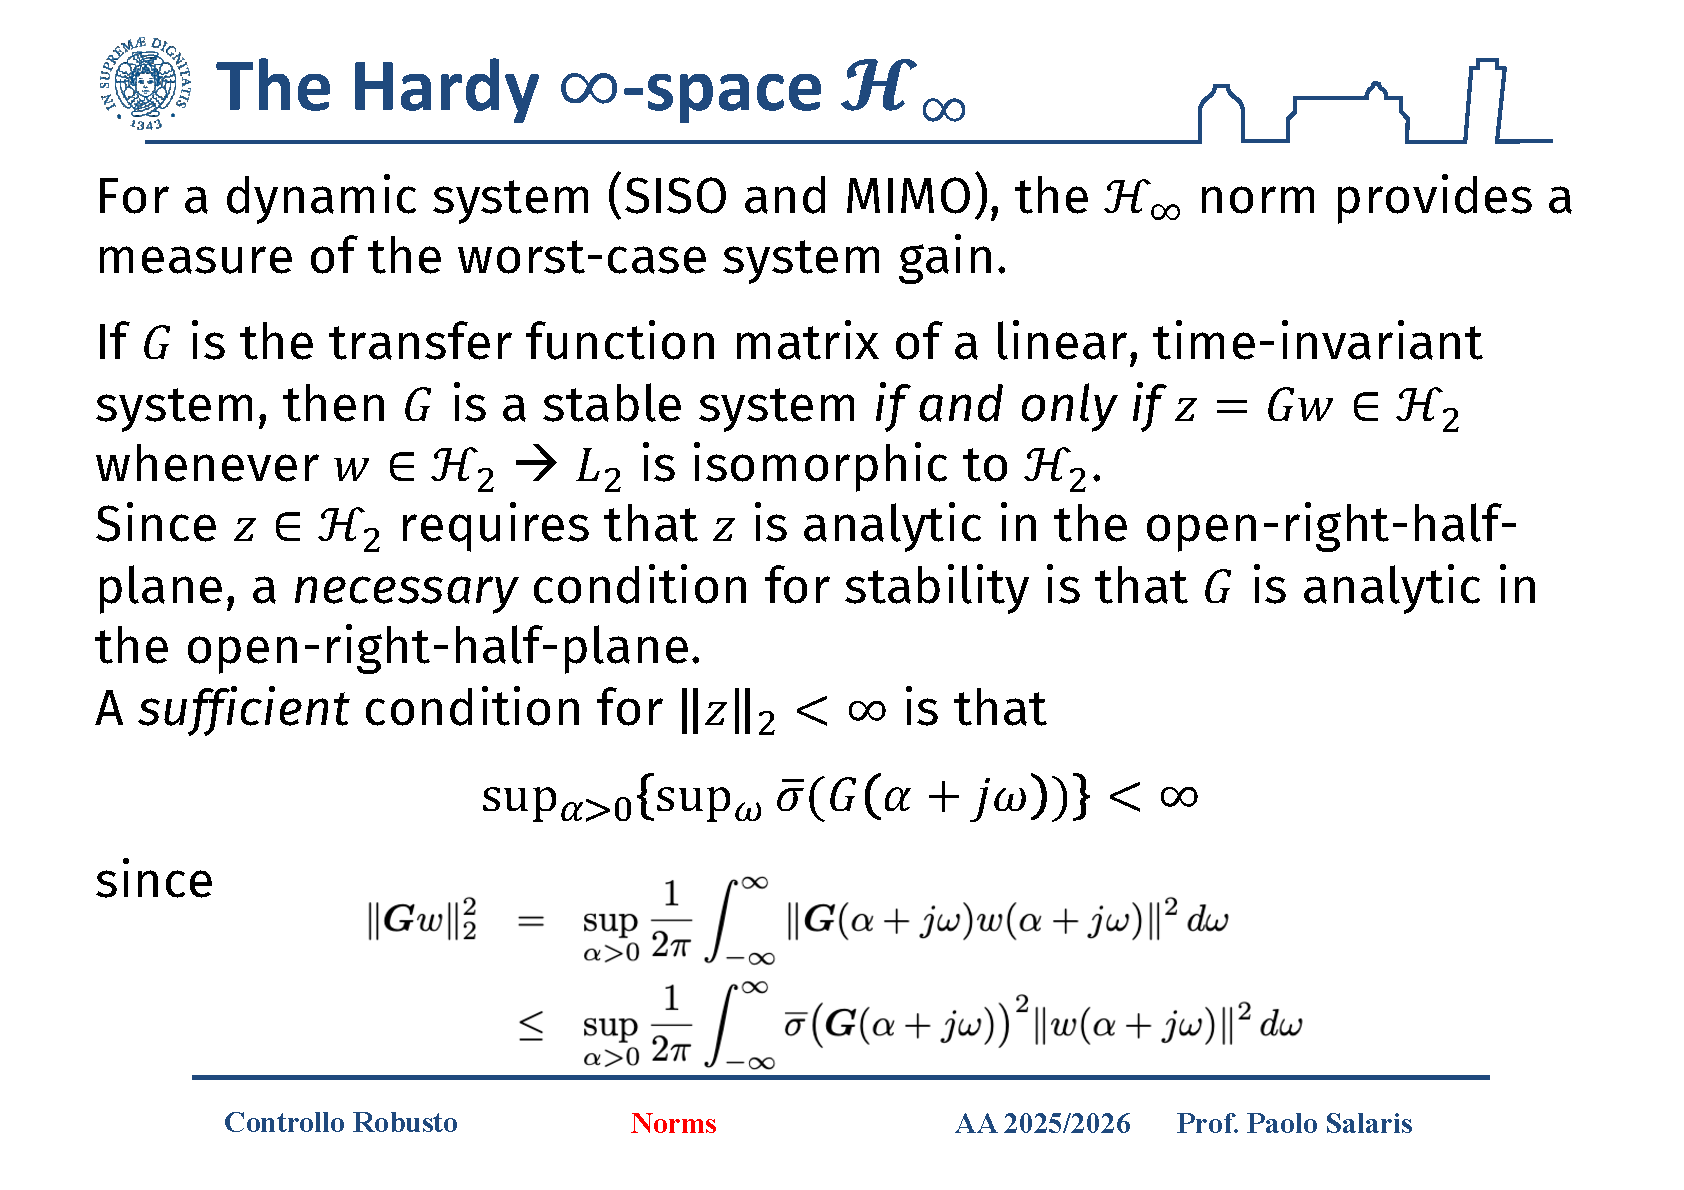
\includegraphics[width=0.78\textwidth]{images8/norms-new-33-53-005.png}
\vfill
\begin{focusbox}
\textbf{Obiettivo del documento.} Questa parte del testo segue le slide 33--53 del PDF aggiornato ``Norms for signals and systems''. La lezione completa prima il calcolo della norma $H_2$ tramite gramiani ed equazioni di Lyapunov; poi introduce la norma $H_\infty$ come guadagno energetico peggiore; infine sviluppa, passo dopo passo, il test Hamiltoniano per verificare se $\|G\|_{H_\infty}<\gamma$. Il filo conduttore resta quello delle slide: ogni formula nuova nasce dalla precedente e serve a trasformare un controllo su infinite frequenze in un problema matriciale finito.
\end{focusbox}
\vfill
{\large Basato sulle slide del corso AA 2025/2026\par}
\end{coverpage}

\section{Lezione 8}

\subsection{Visione d'insieme della lezione}

La Lezione 8 non introduce una lista di risultati indipendenti: costruisce una catena. Le prime slide chiudono il discorso sulla norma $H_2$ mostrando come passare dalla definizione integrale, gi\`a vista nella lezione precedente, a formule calcolabili tramite la rappresentazione di stato. Le slide successive cambiano metrica e introducono la norma $H_\infty$, cio\`e la misura del massimo guadagno energetico del sistema. L'ultimo blocco spiega perch\'e il test
$$
\|G\|_{H_\infty}<\gamma
$$
pu\`o essere trasformato in un controllo sugli autovalori di una matrice Hamiltoniana.

L'ordine delle slide \`e importante. Prima si vede che l'$H_2$ \`e una norma ``di accumulo'': integra l'energia della risposta impulsiva e per questo si collega naturalmente ai gramiani. Poi si vede che l'$H_\infty$ \`e una norma ``di picco'': cerca la frequenza e la direzione d'ingresso che producono l'amplificazione maggiore. Infine, proprio perch\'e cercare un massimo su tutte le frequenze \`e poco pratico, le slide costruiscono un criterio alternativo: fissata una soglia $\gamma$, si verifica se il grafico dei valori singolari resta sempre sotto quella soglia senza campionare direttamente tutte le frequenze.

\begin{keybox}
La domanda dell'$H_2$ \`e: quanta energia complessiva trasferisce il sistema quando viene eccitato impulsivamente? La domanda dell'$H_\infty$ \`e: qual \`e il massimo guadagno possibile, nella frequenza e nella direzione peggiore? Il resto della lezione serve a rendere calcolabili queste due domande.
\end{keybox}

\subsection{Norma \texorpdfstring{$H_2$}{H2} e gramiani}

\subsubsection{Dalla rappresentazione di stato alla risposta impulsiva}

La slide 33 riparte dalla definizione frequenziale della norma $H_2$. Nel caso SISO si integra il modulo quadro di $G(j\omega)$, mentre nel caso MIMO si integra la traccia del prodotto
$$
G^T(-j\omega)G(j\omega),
$$
che, sull'asse immaginario e per sistemi reali, gioca il ruolo di $G^*(j\omega)G(j\omega)$. Queste formule sono corrette, ma non sempre comode: richiedono un integrale su tutte le frequenze. La slide propone quindi di calcolare la stessa quantit\`a nel dominio del tempo, partendo da una realizzazione di stato stabile e strettamente propria:
$$
\dot x(t)=Ax(t)+Bu(t),
\qquad
z(t)=Cx(t),
$$
e matrice di trasferimento
$$
G(s)=C(sI-A)^{-1}B.
$$
L'ipotesi di stabilit\`a significa che $A$ \`e di Hurwitz: tutti i modi naturali decadono e gli integrali che compariranno sono finiti.

Integrando l'equazione di stato fra $0$ e $t$ si ottiene
$$
x(t)=e^{At}x(0)+\int_0^t e^{A(t-\tau)}Bu(\tau)\,d\tau,
$$
e quindi
$$
z(t)=Ce^{At}x(0)+\int_0^t Ce^{A(t-\tau)}Bu(\tau)\,d\tau.
$$
La parte che moltiplica l'ingresso sotto integrale \`e il nucleo di convoluzione del sistema. Per questo le slide definiscono la risposta impulsiva
$$
H(t)=
\begin{cases}
Ce^{At}B, & t>0,\\
0, & t<0.
\end{cases}
$$
La notazione $H(t)$ \`e la stessa risposta impulsiva indicata altrove con $g(t)$; qui \`e utile perch\'e rende subito visibile il legame con $A$, $B$ e $C$. Il passaggio concettuale della slide \`e questo: se $H(t)=Ce^{At}B$, allora l'energia della risposta impulsiva pu\`o essere riscritta come un integrale di matrici di stato.

\begin{figure}[H]
    \centering
    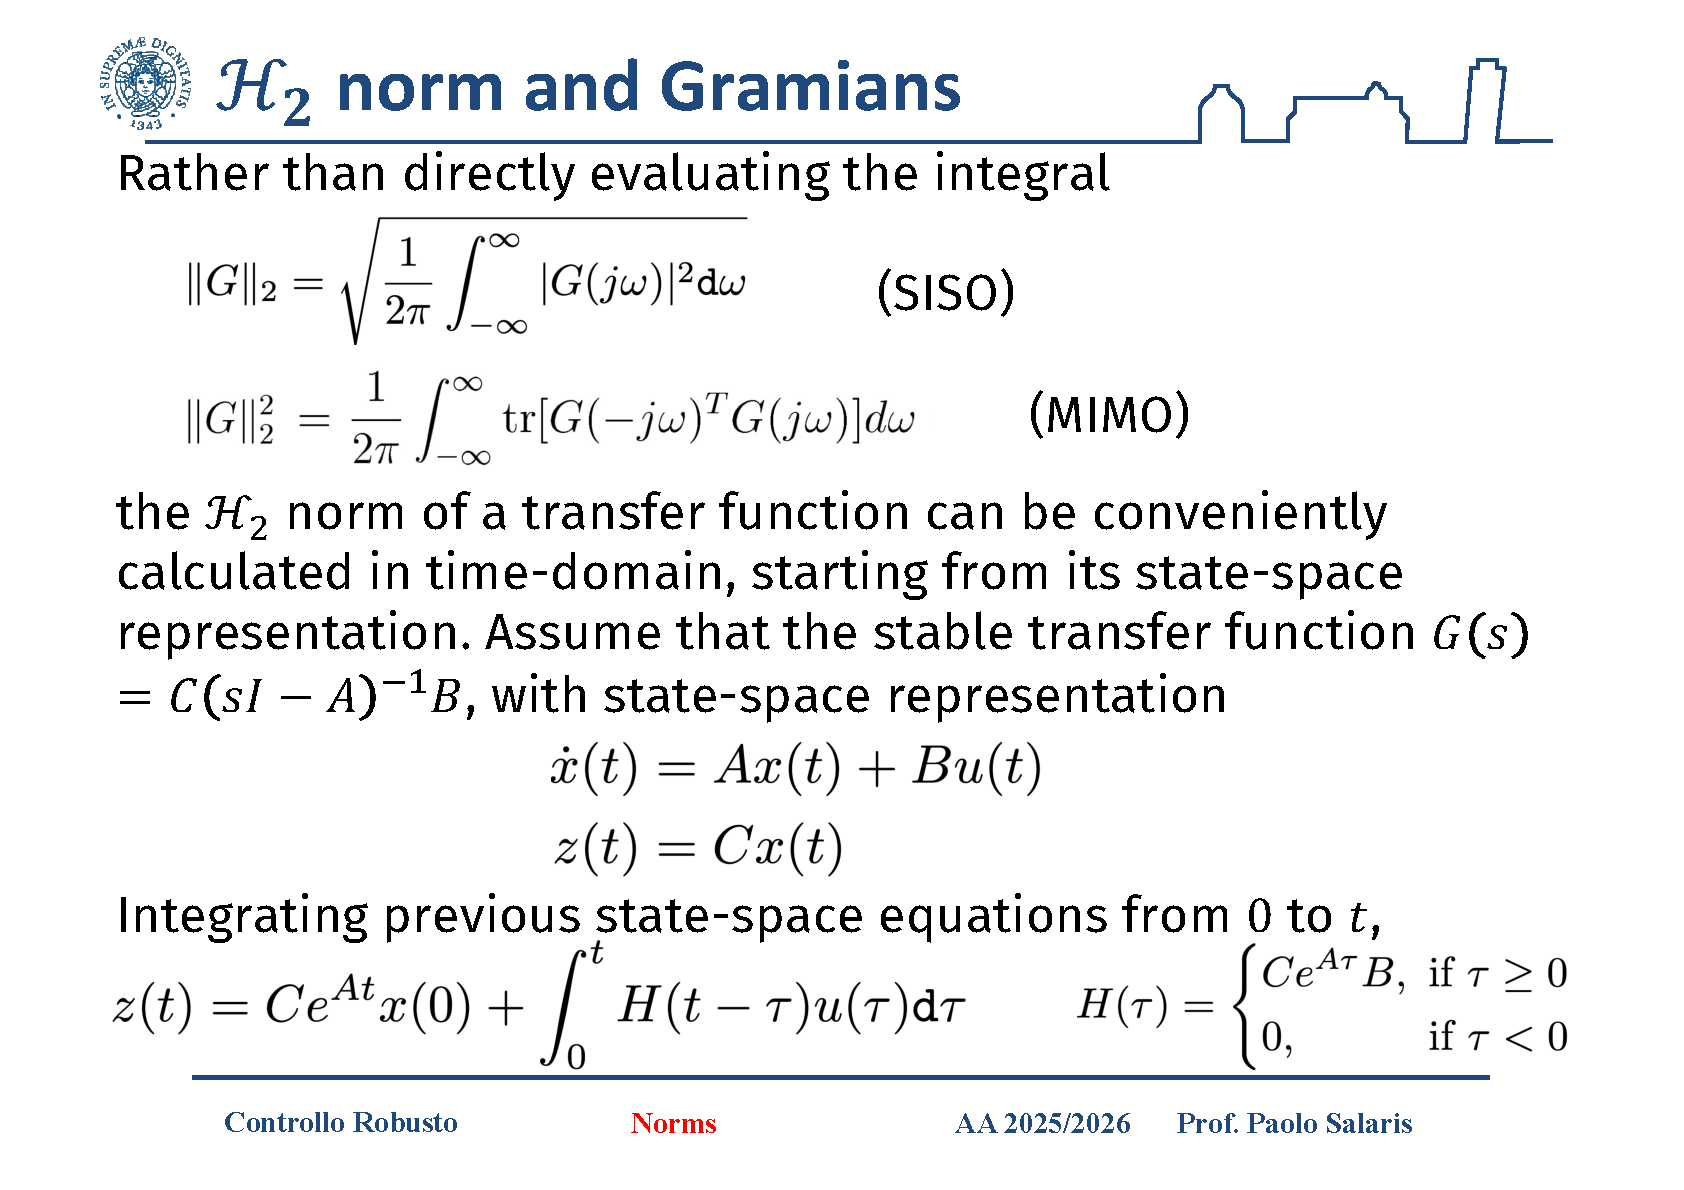
\includegraphics[width=0.82\textwidth]{images8/norms-new-33-53-001.png}
    \caption{La risposta impulsiva di un sistema stabile si ricava direttamente dalla rappresentazione di stato come $H(t)=Ce^{At}B$.}
\end{figure}

\subsubsection{Formula della norma \texorpdfstring{$H_2$}{H2} tramite gramiano di controllabilit\`a}

La slide 34 sostituisce $H(t)=Ce^{At}B$ nella definizione temporale della norma:
$$
\|G\|_{H_2}^2
=
\int_0^\infty \operatorname{tr}\!\bigl(H(t)H^T(t)\bigr)\,dt,
$$
ottenendo
$$
\|G\|_{H_2}^2
=
\int_0^\infty \operatorname{tr}\!\bigl(Ce^{At}BB^Te^{A^Tt}C^T\bigr)\,dt.
$$
Ora si usa la propriet\`a ciclica della traccia: dentro una traccia i fattori possono essere ruotati senza cambiare il valore. Quindi l'integrale pu\`o essere letto come
$$
\|G\|_{H_2}^2
=
\operatorname{tr}\!\left(
C
\left[
\int_0^\infty e^{At}BB^Te^{A^Tt}\,dt
\right]
C^T
\right).
$$
Il termine tra parentesi quadre \`e il gramiano di controllabilit\`a:
$$
W_c
=
\int_0^\infty e^{At}BB^Te^{A^Tt}\,dt,
$$
cos\`\i\ da ottenere la formula compatta
$$
\|G\|_{H_2}^2=\operatorname{tr}(CW_cC^T).
$$

Questa non \`e solo una scorciatoia algebrica. Il gramiano $W_c$ misura quanta energia di stato pu\`o essere generata dagli ingressi attraverso $B$, tenendo conto della dinamica $e^{At}$. La matrice $C$ prende poi quella energia di stato e la proietta sull'uscita $z$. Per questo la formula dice esattamente: energia immessa nello stato, filtrata dalla dinamica, osservata in uscita.

\subsubsection{Formula tramite gramiano di osservabilit\`a}

La stessa slide mostra subito la forma duale. Invece di raggruppare l'integrale attorno a $BB^T$, si ruotano i fattori della traccia in modo da isolare $C^TC$:
$$
W_o
=
\int_0^\infty e^{A^Tt}C^TCe^{At}\,dt,
$$
si ottiene infatti
$$
\|G\|_{H_2}^2=\operatorname{tr}(B^TW_oB).
$$

Le due formule
$$
\|G\|_{H_2}^2=\operatorname{tr}(CW_cC^T)
\qquad\text{e}\qquad
\|G\|_{H_2}^2=\operatorname{tr}(B^TW_oB)
$$
sono la stessa quantit\`a vista da due lati. La formula con $W_c$ dice: guarda quanto gli ingressi riescono a riempire lo stato e poi osserva quello stato con $C$. La formula con $W_o$ dice: guarda quanto ogni stato sarebbe visibile in uscita e poi pesa gli stati effettivamente eccitati da $B$. Le slide stanno preparando cos\`\i\ l'idea che le norme di sistema non dipendono solo dai poli, ma anche da come ingressi e uscite si accoppiano ai modi interni.

\begin{figure}[H]
    \centering
    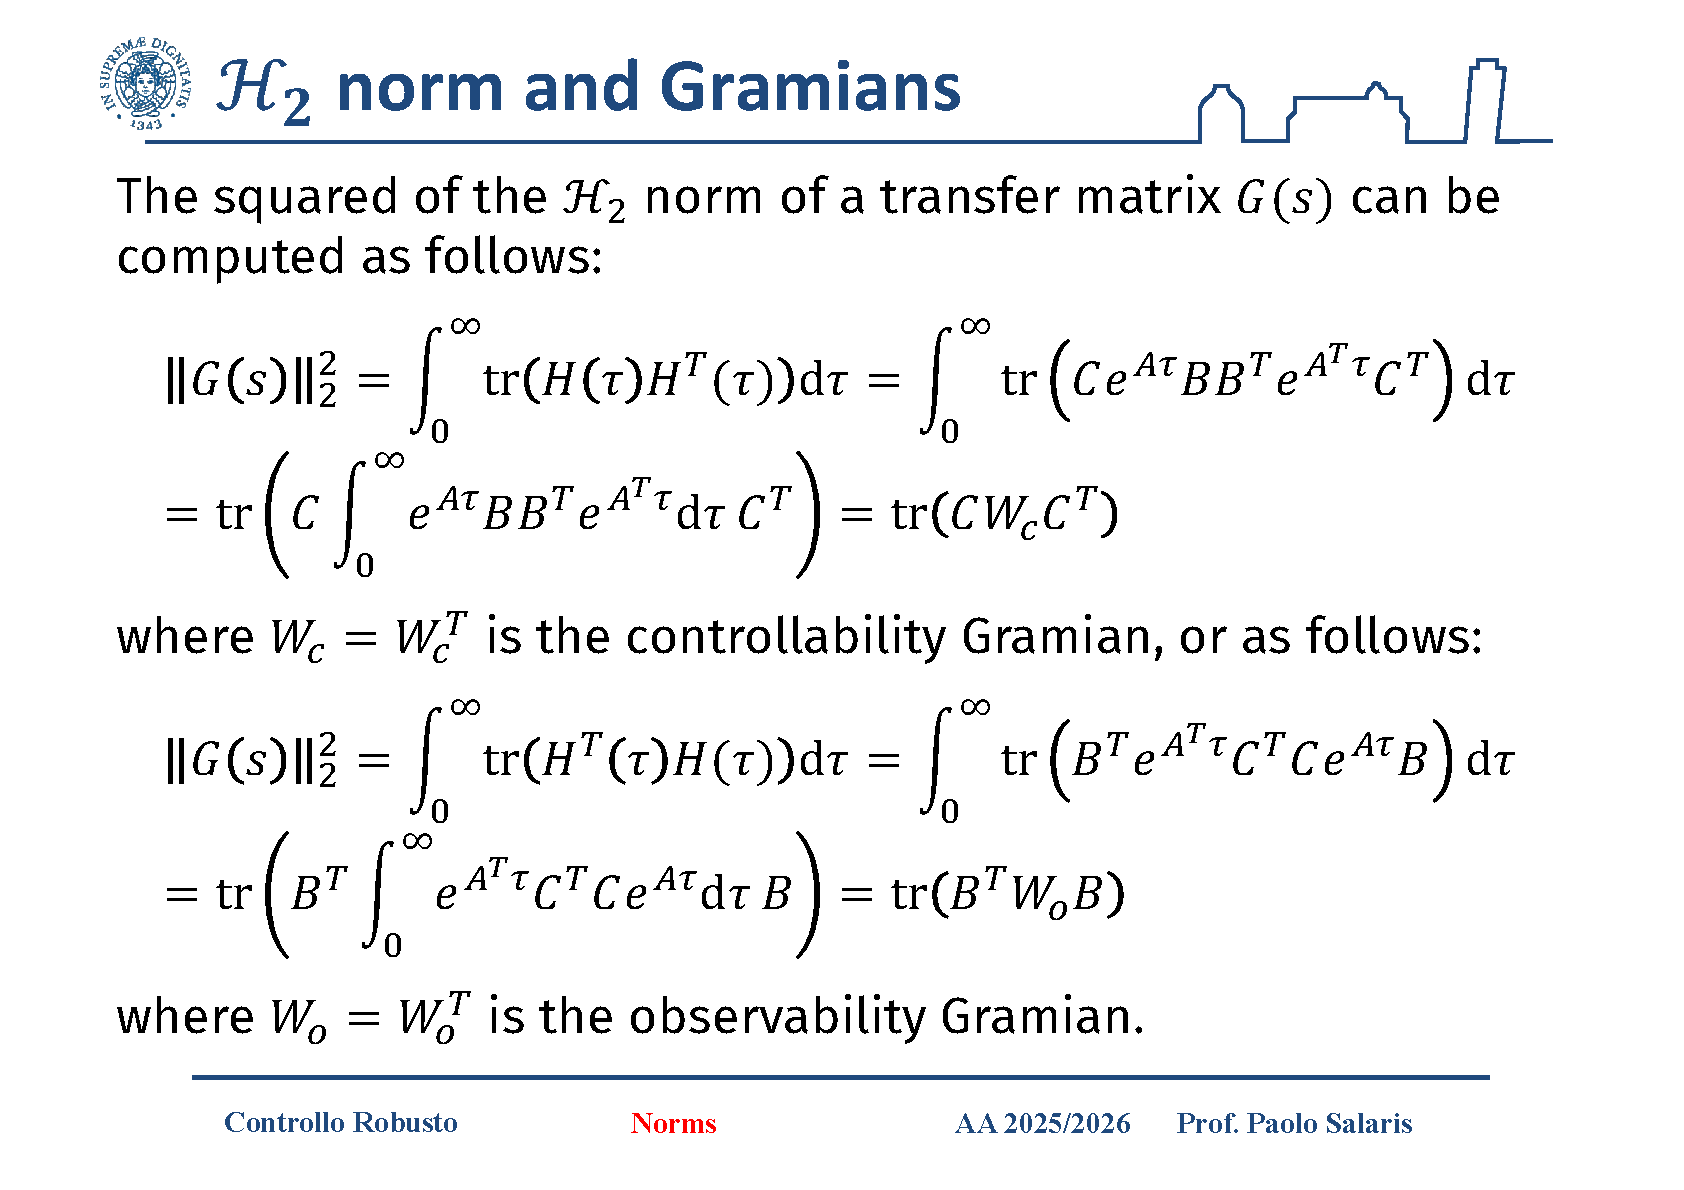
\includegraphics[width=0.82\textwidth]{images8/norms-new-33-53-002.png}
    \caption{La norma $H_2$ pu\`o essere espressa sia con il gramiano di controllabilit\`a sia con quello di osservabilit\`a.}
\end{figure}

\begin{focusbox}
\textbf{Lettura strutturale.} Un modo interno pu\`o essere molto stabile ma quasi invisibile in uscita, oppure facile da osservare ma poco eccitabile dagli ingressi. I gramiani quantificano proprio questa geometria: raggiungibilit\`a e osservabilit\`a diventano grandezze energetiche, non solo propriet\`a booleane.
\end{focusbox}

\subsubsection{Equazioni di Lyapunov}

Le slide 35 e 36 spiegano il passaggio successivo: i gramiani non si calcolano necessariamente tramite integrali impropri. Se $A$ \`e di Hurwitz, essi sono le soluzioni delle equazioni di Lyapunov
$$
A^TW_o+W_oA+C^TC=0,
$$
$$
AW_c+W_cA^T+BB^T=0.
$$
Vediamo il passaggio per $W_o$, che \`e quello mostrato nelle slide. Dalla definizione
$$
W_o=\int_0^\infty e^{A^T\tau}C^TCe^{A\tau}\,d\tau
$$
si moltiplica a sinistra per $e^{A^Tt_0}$ e a destra per $e^{At_0}$:
$$
e^{A^Tt_0}W_oe^{At_0}
=
\int_0^\infty e^{A^T(t_0+\tau)}C^TCe^{A(t_0+\tau)}\,d\tau.
$$
Cambiando variabile $\theta=t_0+\tau$, questa diventa
$$
e^{A^Tt_0}W_oe^{At_0}
=
\int_{t_0}^\infty e^{A^T\theta}C^TCe^{A\theta}\,d\theta.
$$
Ora si differenzia rispetto a $t_0$. Il lato sinistro d\`a
$$
A^Te^{A^Tt_0}W_oe^{At_0}
+e^{A^Tt_0}W_oe^{At_0}A,
$$
mentre il lato destro, per la regola di derivazione di un integrale con estremo variabile, d\`a
$$
-e^{A^Tt_0}C^TCe^{At_0}.
$$
Ponendo $t_0=0$ si ottiene
$$
A^TW_o+W_oA=-C^TC,
$$
cio\`e
$$
A^TW_o+W_oA+C^TC=0.
$$
Il ragionamento per $W_c$ \`e analogo e produce
$$
AW_c+W_cA^T+BB^T=0.
$$

Il punto concettuale \`e essenziale: la stabilit\`a di $A$ permette di sostituire un integrale infinito con un'equazione matriciale lineare. In pratica, quindi, il calcolo di $\|G\|_{H_2}$ diventa:
\begin{enumerate}
    \item risolvere una Lyapunov per $W_c$ oppure per $W_o$;
    \item calcolare la traccia corrispondente;
    \item prendere la radice quadrata.
\end{enumerate}

La slide 36 richiama anche il comando \texttt{lyap} di \textsc{Matlab}. Il dettaglio \`e pratico ma significativo: l'obiettivo di questo blocco non \`e solo dare una formula elegante, ma arrivare a un metodo di calcolo stabile e standard.

\begin{figure}[H]
    \centering
    \begin{subfigure}{0.48\textwidth}
        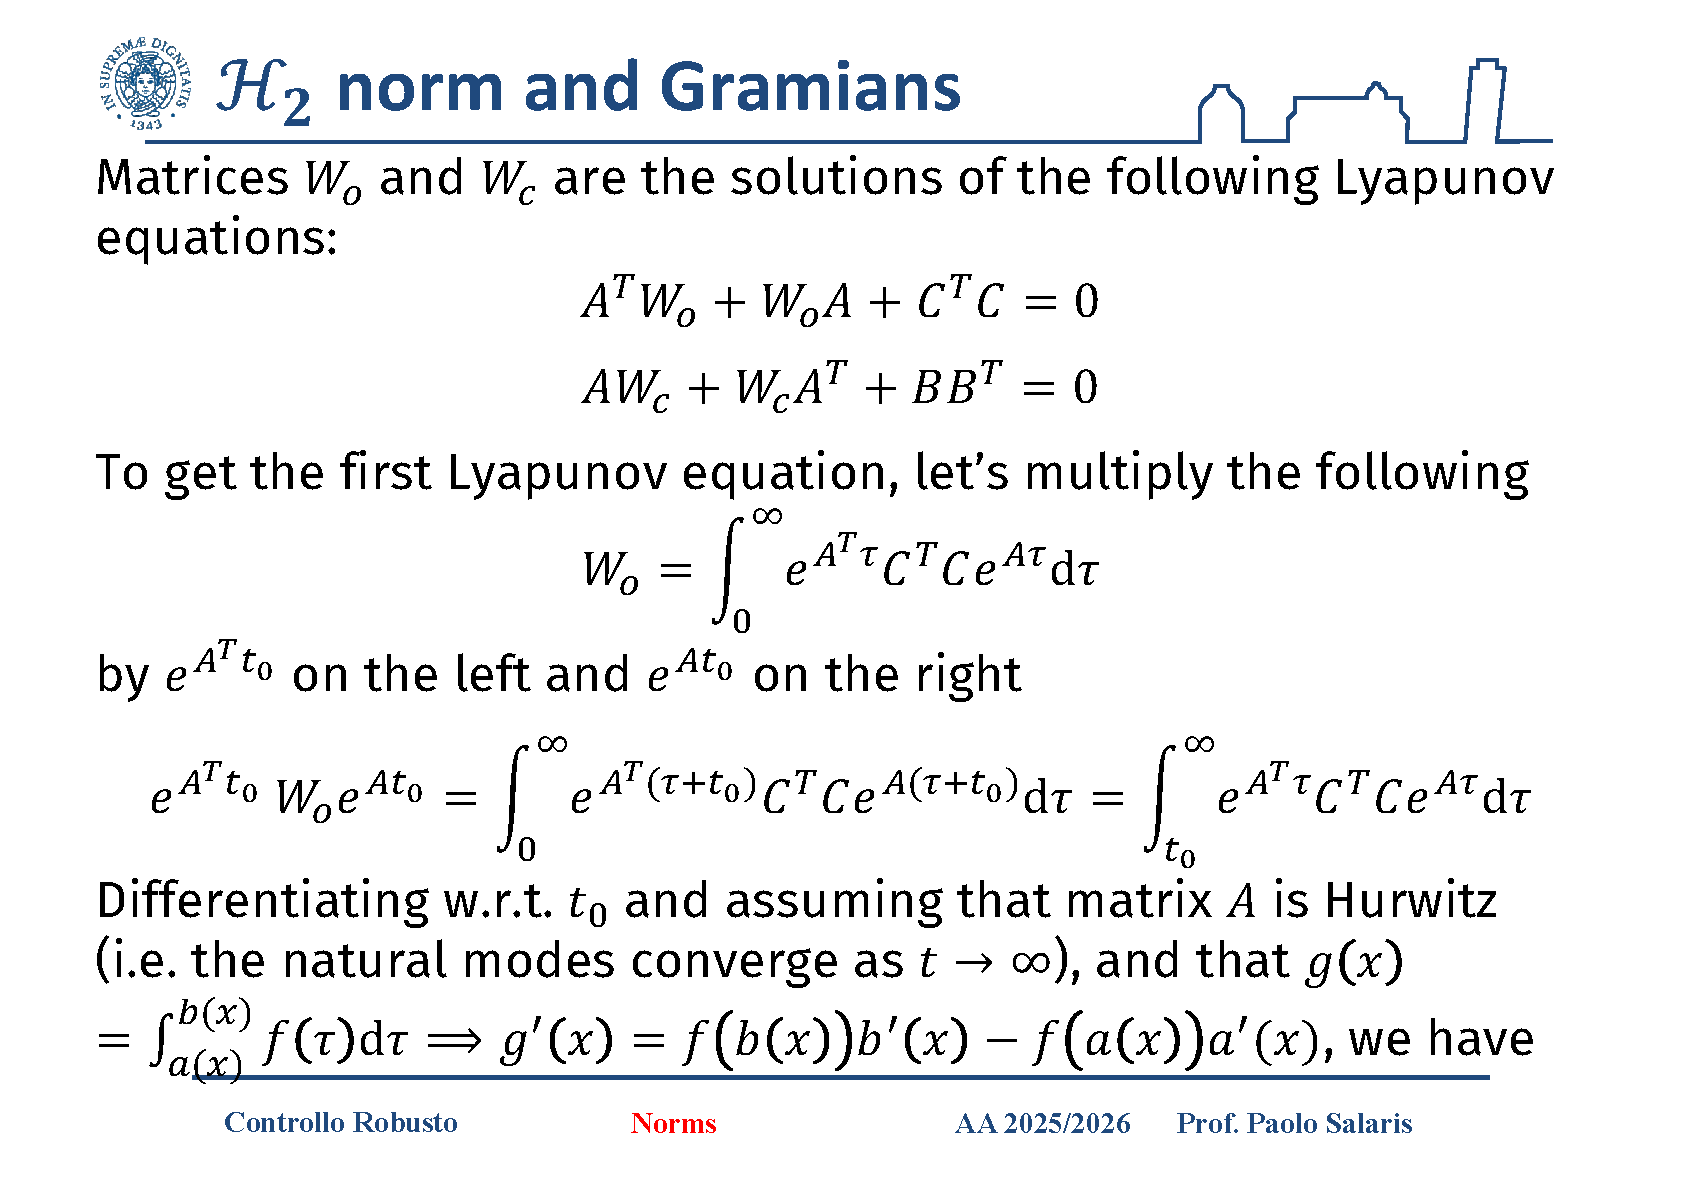
\includegraphics[width=\linewidth]{images8/norms-new-33-53-003.png}
        \caption{Derivazione dell'equazione di Lyapunov a partire dalla definizione integrale del gramiano.}
    \end{subfigure}
    \hfill
    \begin{subfigure}{0.48\textwidth}
        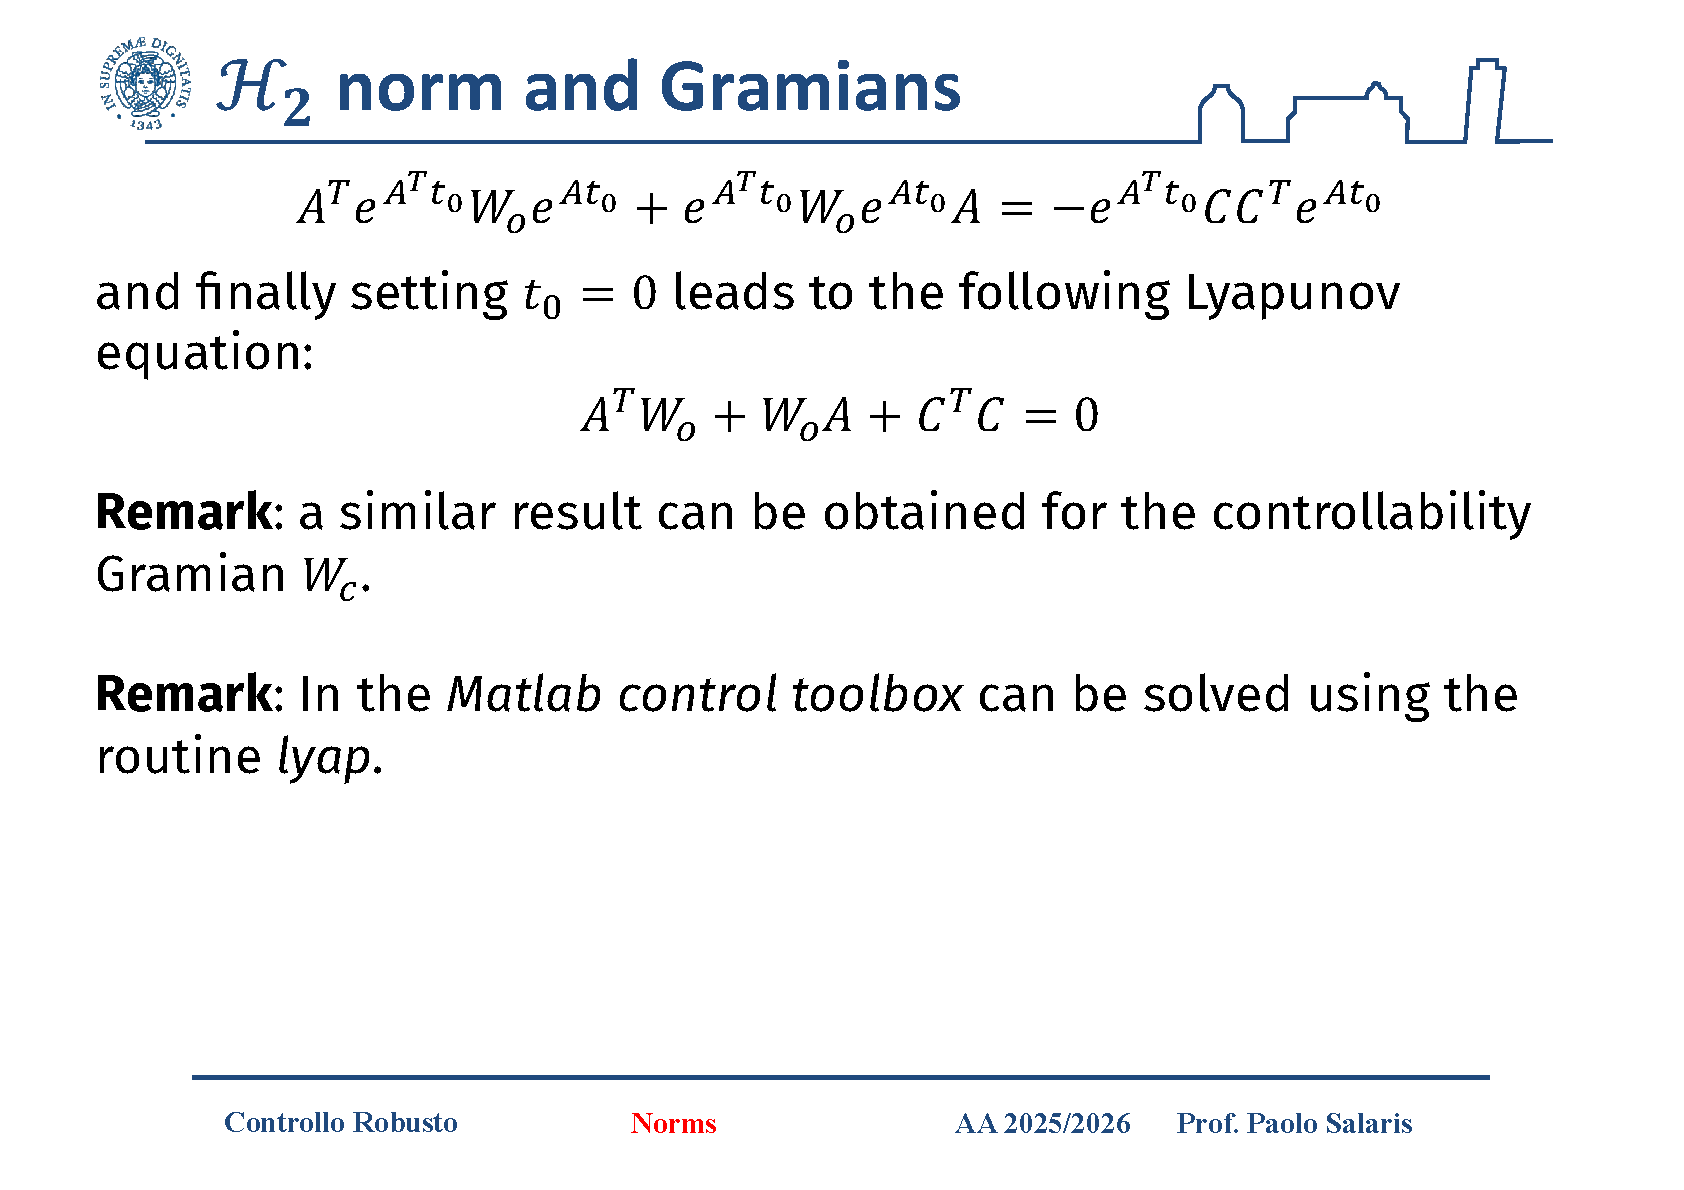
\includegraphics[width=\linewidth]{images8/norms-new-33-53-004.png}
        \caption{Forma finale delle equazioni di Lyapunov e richiamo all'uso pratico del comando `lyap`.}
    \end{subfigure}
    \caption{I gramiani trasformano il calcolo della norma $H_2$ in un problema di algebra lineare numericamente ben posto.}
\end{figure}

\subsection{Lo spazio di Hardy \texorpdfstring{$H_\infty$}{Hinf}}

\subsubsection{Norma \texorpdfstring{$H_\infty$}{Hinf} come guadagno peggiore}

La slide 37 apre la seconda parte con una frase molto precisa: per sistemi dinamici SISO e MIMO, la norma $H_\infty$ misura il \emph{worst-case system gain}. Quindi non stiamo pi\`u chiedendo quanta energia complessiva compare nella risposta impulsiva, come per l'$H_2$; stiamo chiedendo quanto il sistema pu\`o amplificare nel caso pi\`u sfavorevole.

Le slide introducono questa idea passando dallo spazio di Hardy $H_\infty$. Con la convenzione usata nel corso, si considerano funzioni analitiche nel semipiano destro aperto e limitate in quel semipiano. Per una matrice di trasferimento $G(s)$ si definisce
$$
\|G\|_{H_\infty}
=
\sup_{a>0}\sup_{\omega}\,\bar{\sigma}\!\bigl(G(a+j\omega)\bigr),
$$
dove $\bar{\sigma}$ \`e il massimo valore singolare. Il parametro $a>0$ serve a guardare le rette verticali interne al dominio di analiticit\`a; poi, per funzioni stabili, il valore della norma pu\`o essere letto sul bordo. Infatti la slide successiva dice che, se $G\in H_\infty$, allora il limite
$$
G(j\omega)=\lim_{a\to 0^+}G(a+j\omega)
$$
esiste per quasi ogni $\omega$ e
$$
\|G\|_{H_\infty}
=
\sup_{\omega\in\mathbb{R}} \bar{\sigma}\!\bigl(G(j\omega)\bigr).
$$
Quando il massimo \`e raggiunto, come accade nei casi razionali stabili pi\`u comuni, si pu\`o sostituire il sup con un max.

Il motivo della definizione si vede dalla disuguaglianza scritta nelle slide. Se $z=Gw$, allora, in frequenza,
$$
\|z\|_2^2
\le
\left(
\sup_{a>0}\sup_\omega \bar{\sigma}^2(G(a+j\omega))
\right)
\|w\|_2^2.
$$
Quindi la quantit\`a $\|G\|_{H_\infty}$ \`e proprio il numero che limita dall'alto il guadagno energetico del sistema. Nel caso SISO \`e il picco di $|G(j\omega)|$; nel caso MIMO \`e il picco, su tutte le frequenze, del massimo valore singolare, cio\`e della direzione d'ingresso amplificata di pi\`u.

\begin{figure}[H]
    \centering
    \begin{subfigure}{0.48\textwidth}
        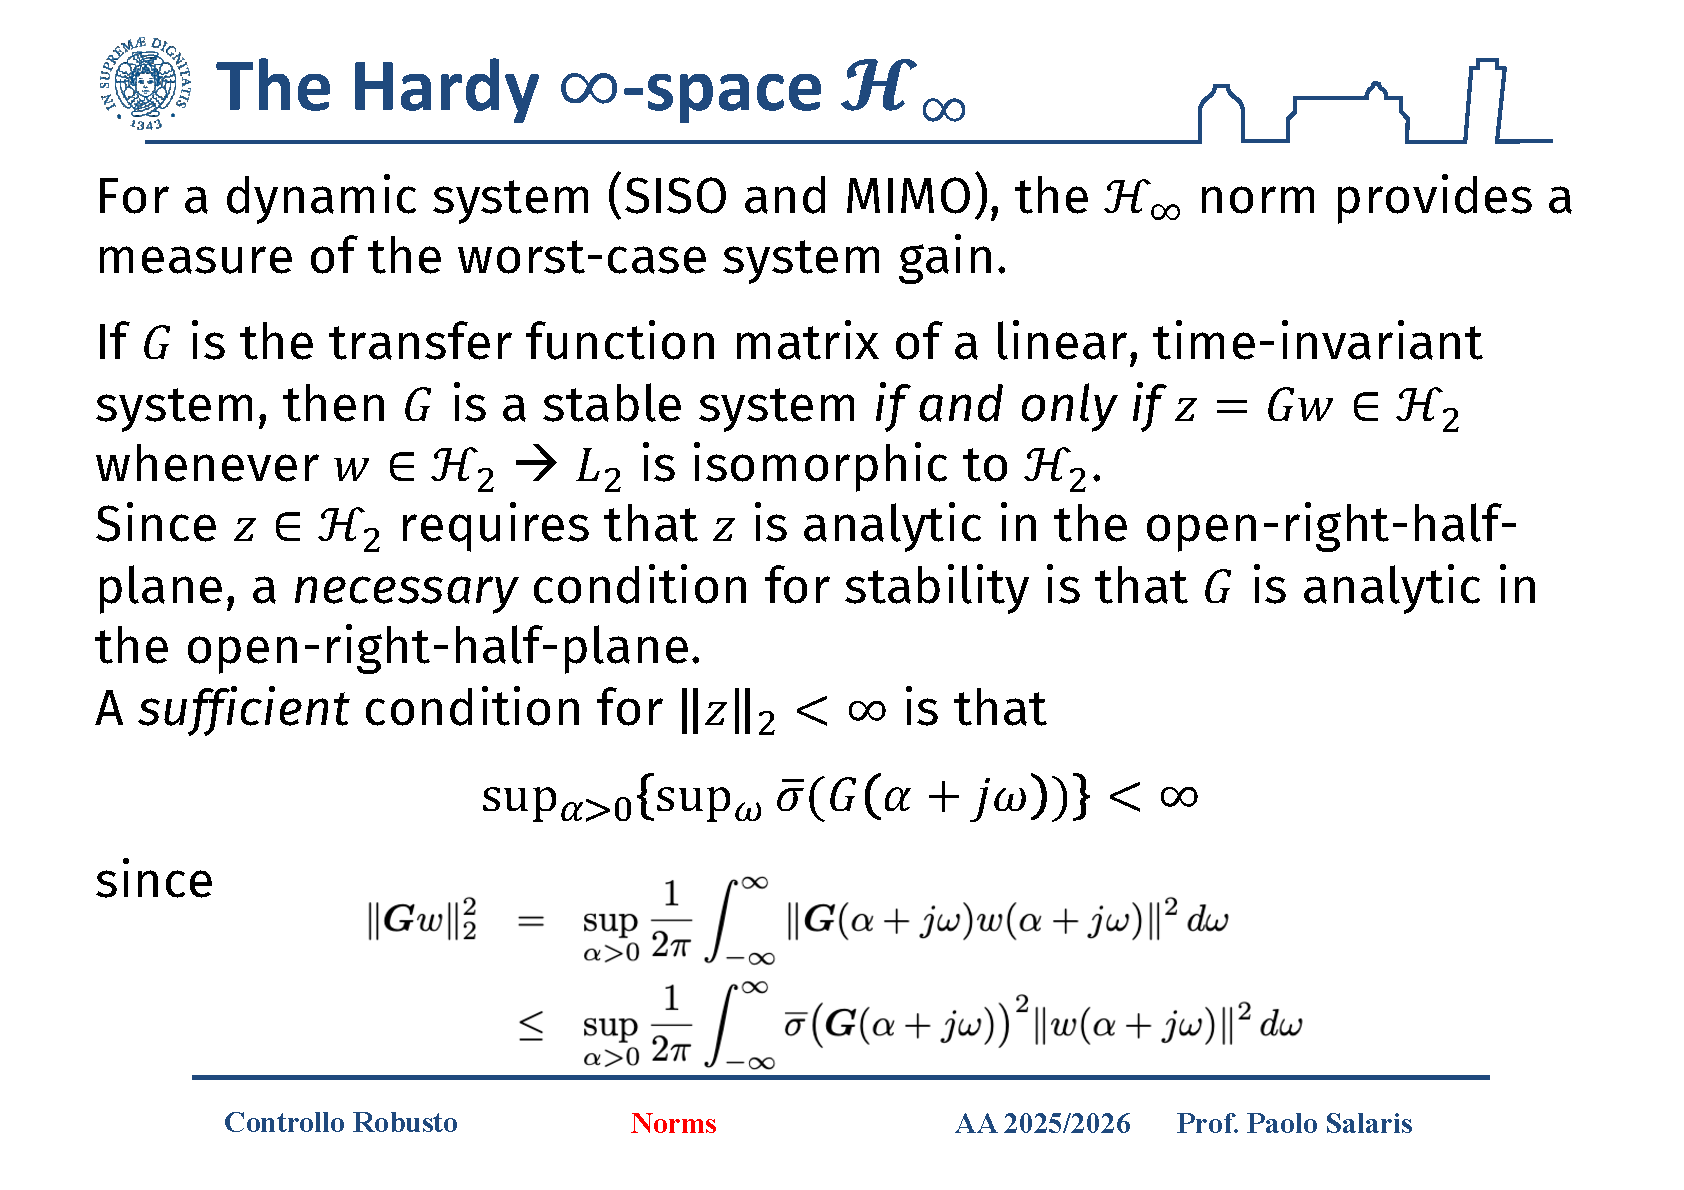
\includegraphics[width=\linewidth]{images8/norms-new-33-53-005.png}
        \caption{Definizione astratta dello spazio di Hardy $H_\infty$ come spazio di funzioni analitiche e limitate.}
    \end{subfigure}
    \hfill
    \begin{subfigure}{0.48\textwidth}
        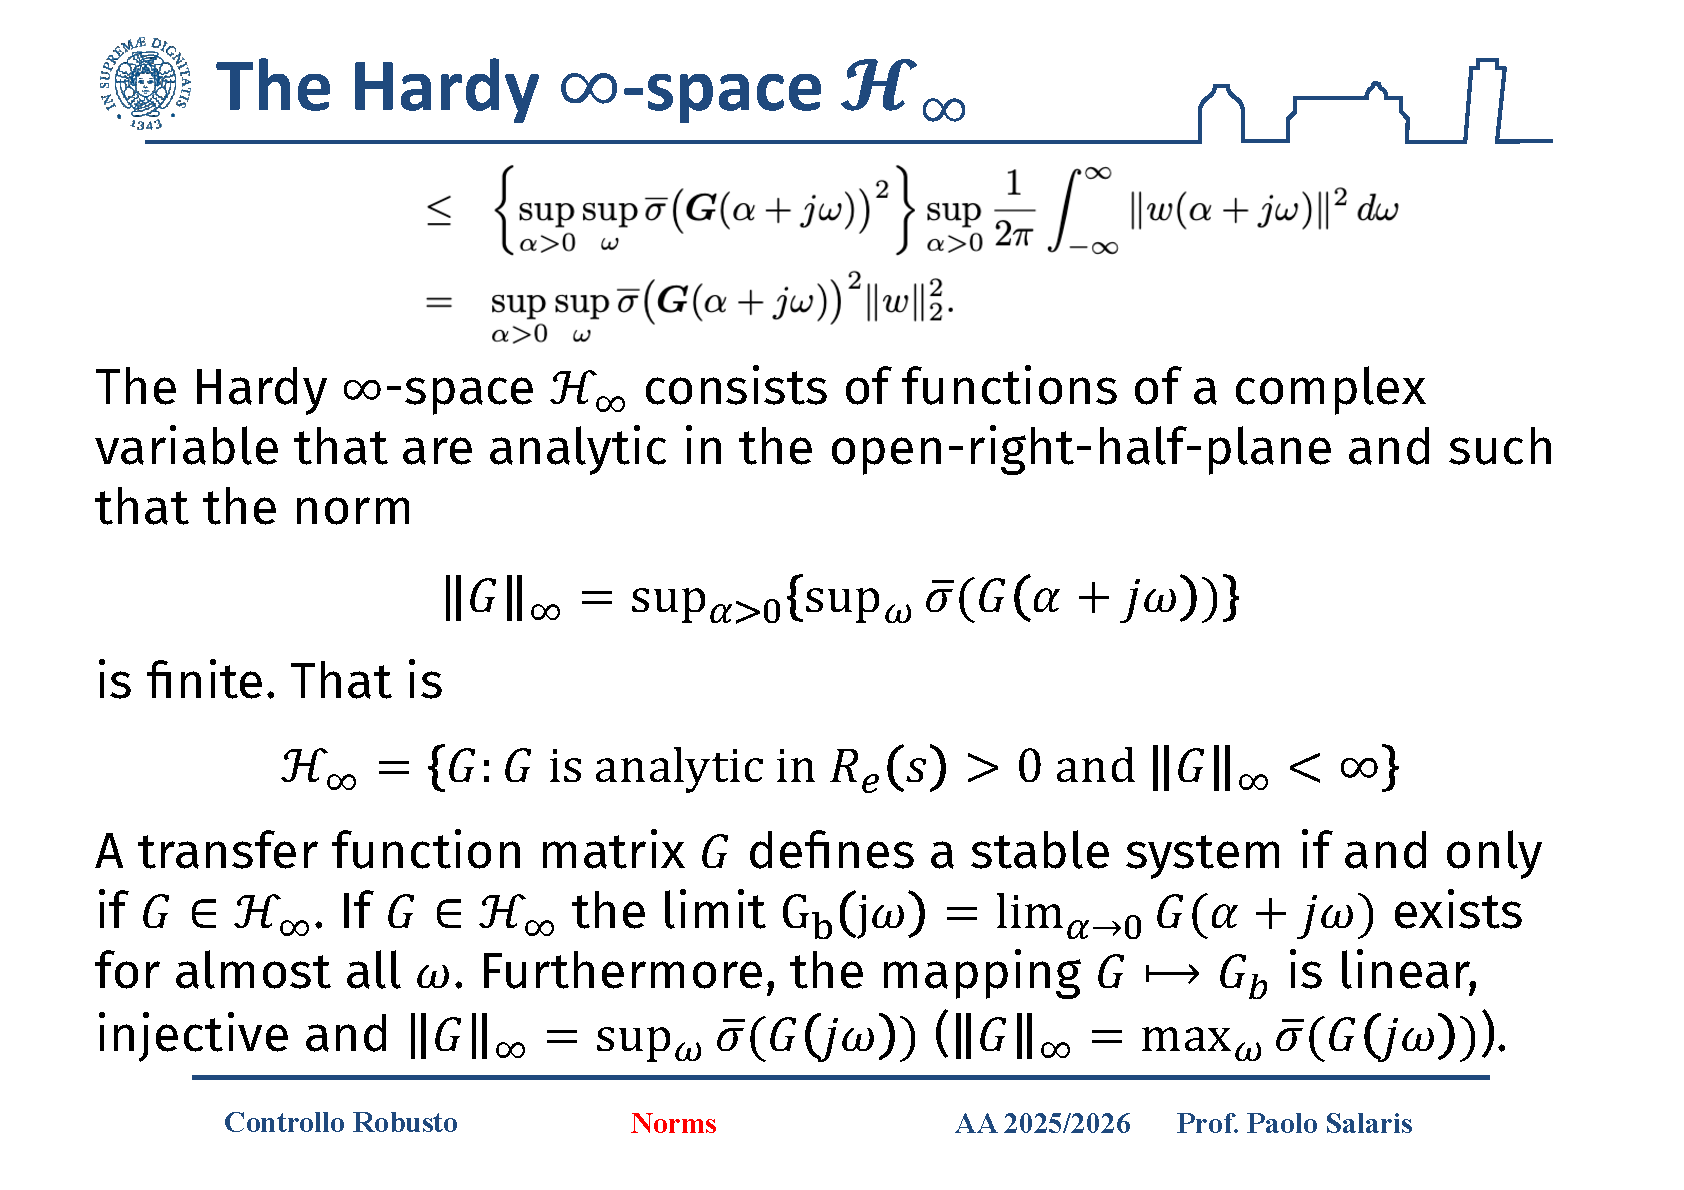
\includegraphics[width=\linewidth]{images8/norms-new-33-53-006.png}
        \caption{Norma $H_\infty$ come estremo superiore del massimo valore singolare al bordo.}
    \end{subfigure}
    \caption{La norma $H_\infty$ misura il guadagno peggiore del sistema, non la sua risposta energetica media.}
\end{figure}

\subsubsection{Interpretazione come norma indotta da \texorpdfstring{$L_2$}{L2} a \texorpdfstring{$L_2$}{L2}}

La slide 39 traduce la definizione in una forma direttamente operativa. Se $G$ \`e razionale, allora $G\in H_\infty$ se e solo se non ha poli nel semipiano destro chiuso. In altre parole, per i sistemi razionali del corso la condizione di appartenenza a $H_\infty$ coincide con la stabilit\`a del sistema.

Per un sistema stabile, la norma $H_\infty$ \`e la norma indotta da $L_2$ a $L_2$:
$$
\|G\|_{H_\infty}
=
\sup_{\|w\|_2=1}\|z\|_2,
\qquad z=Gw.
$$
Equivalentemente,
$$
\|G\|_{H_\infty}
=
\sup_{w\neq 0}\frac{\|z\|_2}{\|w\|_2}.
$$
La frase ``energia gain'' della slide va letta cos\`\i: si considerano tutti gli ingressi a energia finita, si normalizza la loro energia a uno, e si cerca l'uscita a energia massima. Il rapporto peggiore \`e $\|G\|_{H_\infty}$.

La differenza rispetto all'$H_2$ \`e quindi netta:
\begin{itemize}
    \item l'$H_2$ misura una risposta energetica complessiva, ottenuta integrando la risposta impulsiva;
    \item l'$H_\infty$ misura un limite uniforme: nessun ingresso $L_2$ pu\`o essere amplificato pi\`u di quel fattore.
\end{itemize}

Da qui nasce il nome \emph{$H_\infty$ control}: si vogliono imporre obiettivi del tipo ``tieni piccola la norma $H_\infty$ di questo canale chiuso'', naturalmente sotto il vincolo che il ciclo chiuso sia internamente stabile.

\begin{figure}[H]
    \centering
    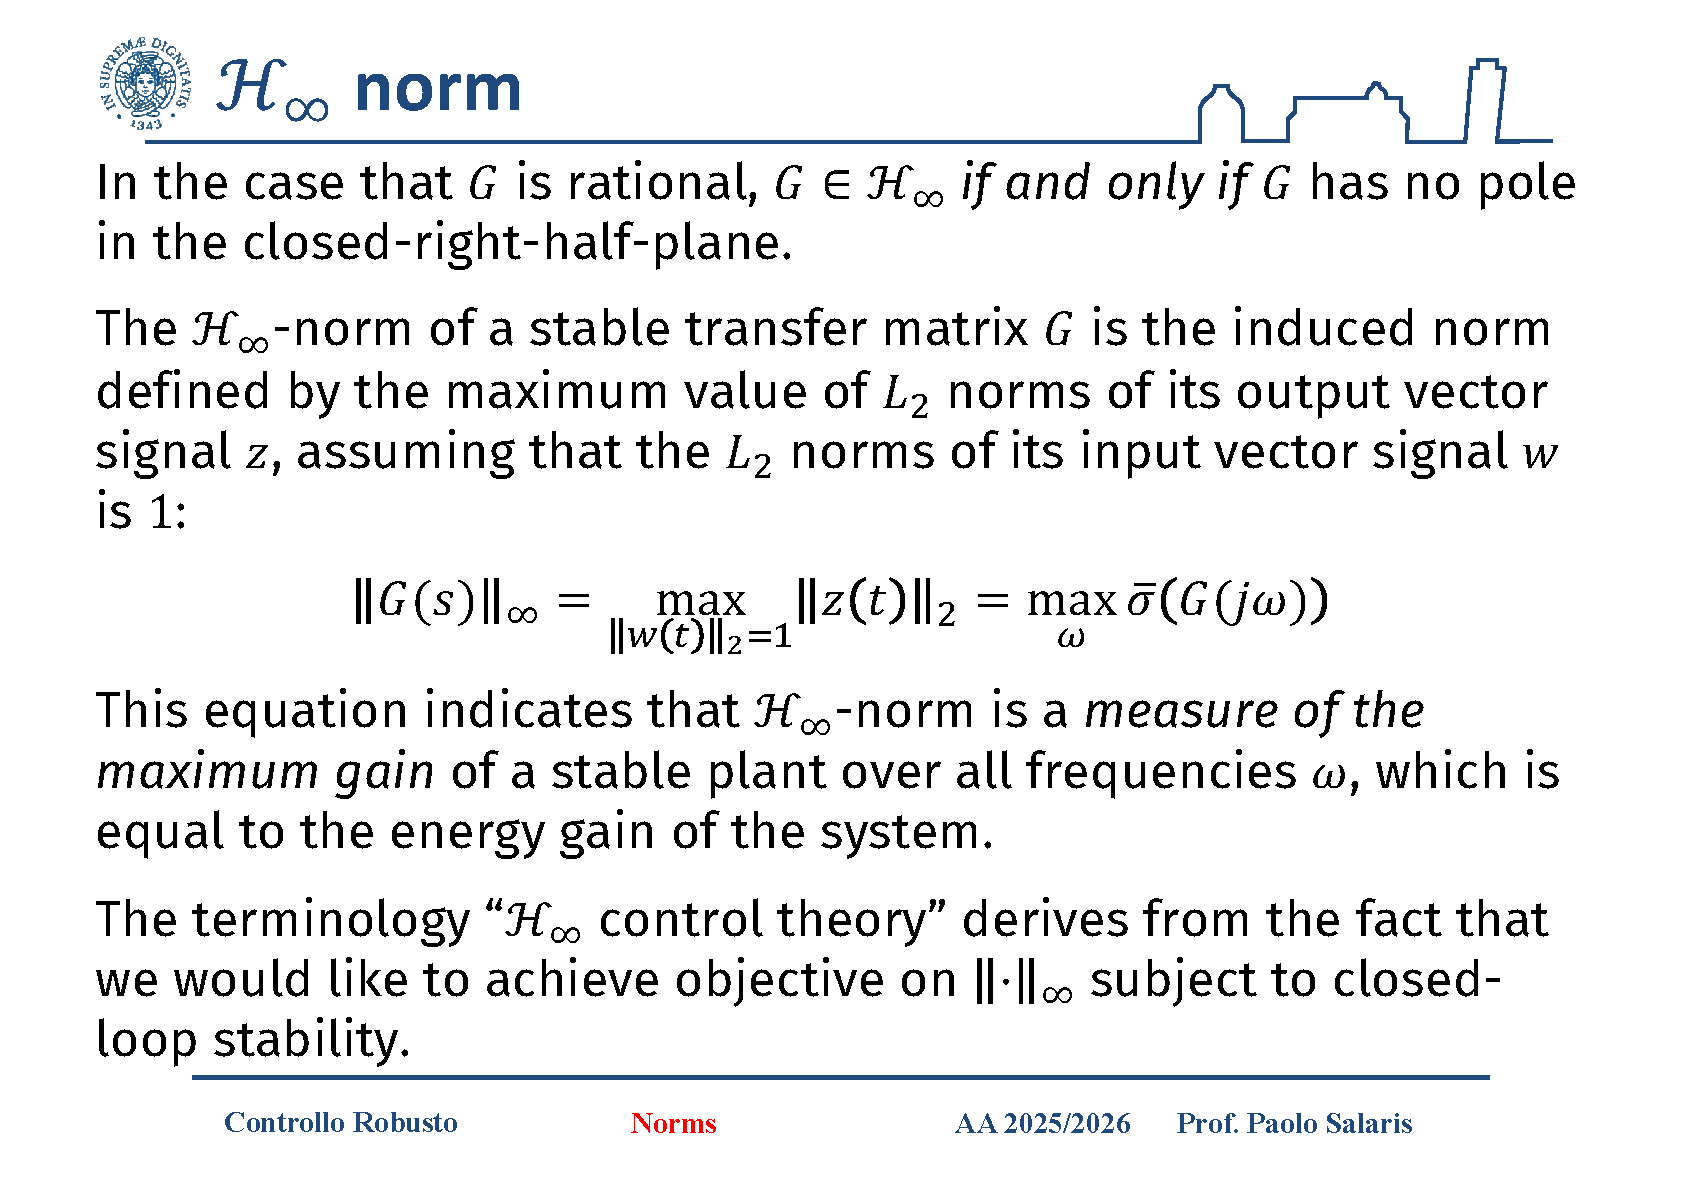
\includegraphics[width=0.82\textwidth]{images8/norms-new-33-53-007.png}
    \caption{La norma $H_\infty$ \`e la norma indotta da $L_2$ a $L_2$ e coincide con il massimo guadagno del sistema.}
\end{figure}

\begin{focusbox}
\textbf{Punto chiave per il controllo robusto.} Una specifica $H_\infty$ non dice che il sistema va bene ``in media'': dice che nessuna frequenza e nessuna direzione d'ingresso pu\`o superare il guadagno imposto. Per questo \`e la metrica naturale delle garanzie di caso peggiore.
\end{focusbox}

\subsection{Perch\'e la norma \texorpdfstring{$H_\infty$}{Hinf} \`e pi\`u difficile da calcolare}

La slide 40 mette in evidenza il salto pratico rispetto all'$H_2$. Per l'$H_2$ abbiamo appena ottenuto una Lyapunov, quindi una procedura algebrica diretta. Per l'$H_\infty$, invece, la norma coincide con il massimo di una funzione di frequenza:
$$
\omega\mapsto \bar{\sigma}(G(j\omega)).
$$
In generale questo massimo non si calcola analiticamente.

Le slide elencano tre strategie:
\begin{enumerate}
    \item tracciare $\bar{\sigma}(G(j\omega))$ in funzione di $\omega$ e cercarne il massimo per ispezione;
    \item scandire numericamente $\omega$ con un calcolatore;
    \item trasformare il problema in una famiglia di test: fissato $\gamma>0$, decidere se $\|G\|_{H_\infty}<\gamma$.
\end{enumerate}

Le prime due strategie sono intuitive, ma la slide insiste su un limite: valutare $\bar{\sigma}(G(j\omega_0))$ in un punto dice solo che
$$
\|G\|_{H_\infty}\ge \bar{\sigma}(G(j\omega_0)).
$$
Non certifica che non esista un picco pi\`u alto tra due frequenze campionate. Per questo la terza strategia \`e pi\`u importante: se sappiamo rispondere in modo affidabile alla domanda ``$\|G\|_{H_\infty}<\gamma$?'', allora possiamo trovare la norma con una ricerca su $\gamma$, ad esempio per bisezione, mantenendo sempre un intervallo
$$
\gamma_{\mathrm{low}}<\|G\|_{H_\infty}<\gamma_{\mathrm{high}}.
$$

La slide 41 spiega anche la lettura nel dominio del tempo. Per il teorema di Parseval, la norma $H_\infty$ pu\`o essere caratterizzata come
$$
\|G\|_{H_\infty}
=
\sup_{v\neq 0}\frac{\|z\|_2}{\|v\|_2},
\qquad z=Gv.
$$
Quindi, fissato $\gamma>0$, la condizione $\|G\|_{H_\infty}<\gamma$ equivale a dire che per ogni ingresso non nullo
$$
\|z\|_2^2-\gamma^2\|v\|_2^2<0.
$$
Le slide lo scrivono come funzionale
$$
J_\infty(G,\gamma)
=
\max_v
\int_0^\infty
\left[
z^T(t)z(t)-\gamma^2v^T(t)v(t)
\right]dt.
$$
Se questo massimo \`e negativo, allora nessun ingresso riesce a produrre un guadagno energetico maggiore di $\gamma$. Il blocco successivo della lezione cerca proprio un test pratico per stabilire questa disuguaglianza.

\begin{figure}[H]
    \centering
    \begin{subfigure}{0.48\textwidth}
        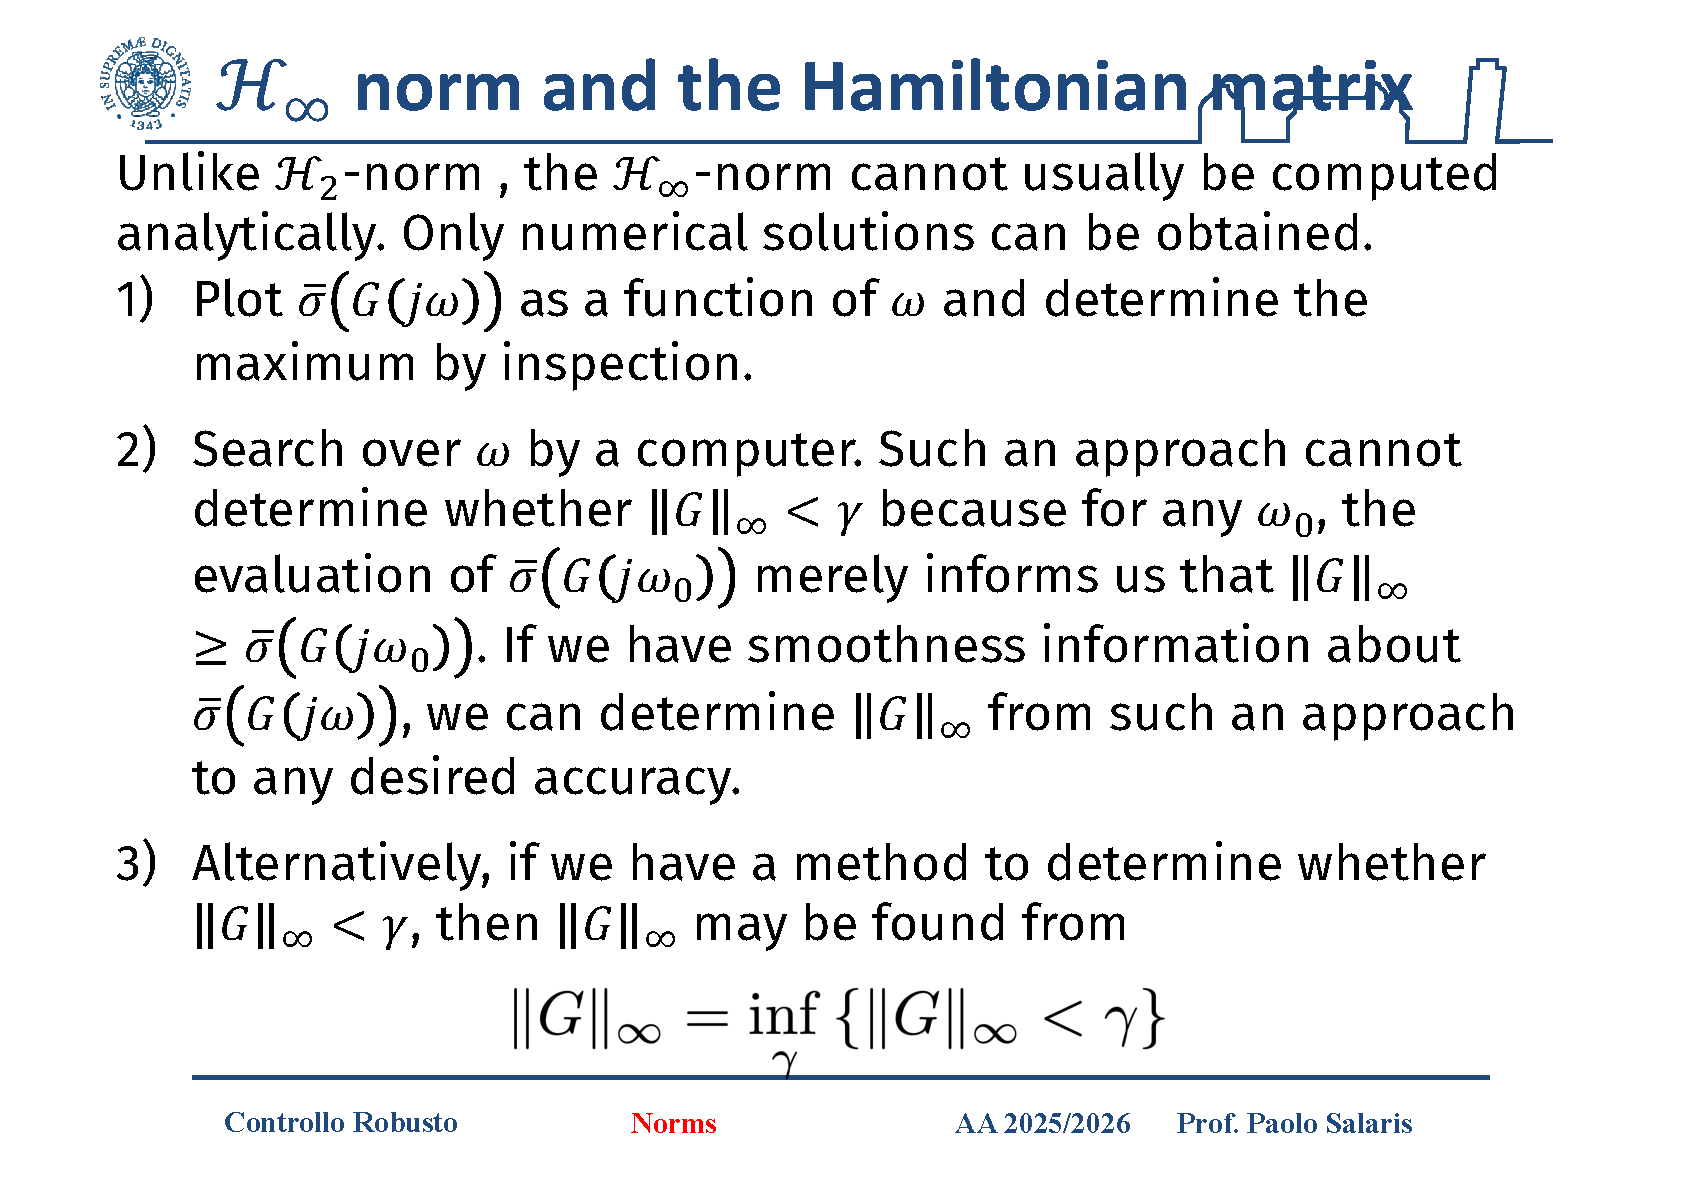
\includegraphics[width=\linewidth]{images8/norms-new-33-53-008.png}
        \caption{Strategie numeriche per determinare la norma $H_\infty$.}
    \end{subfigure}
    \hfill
    \begin{subfigure}{0.48\textwidth}
        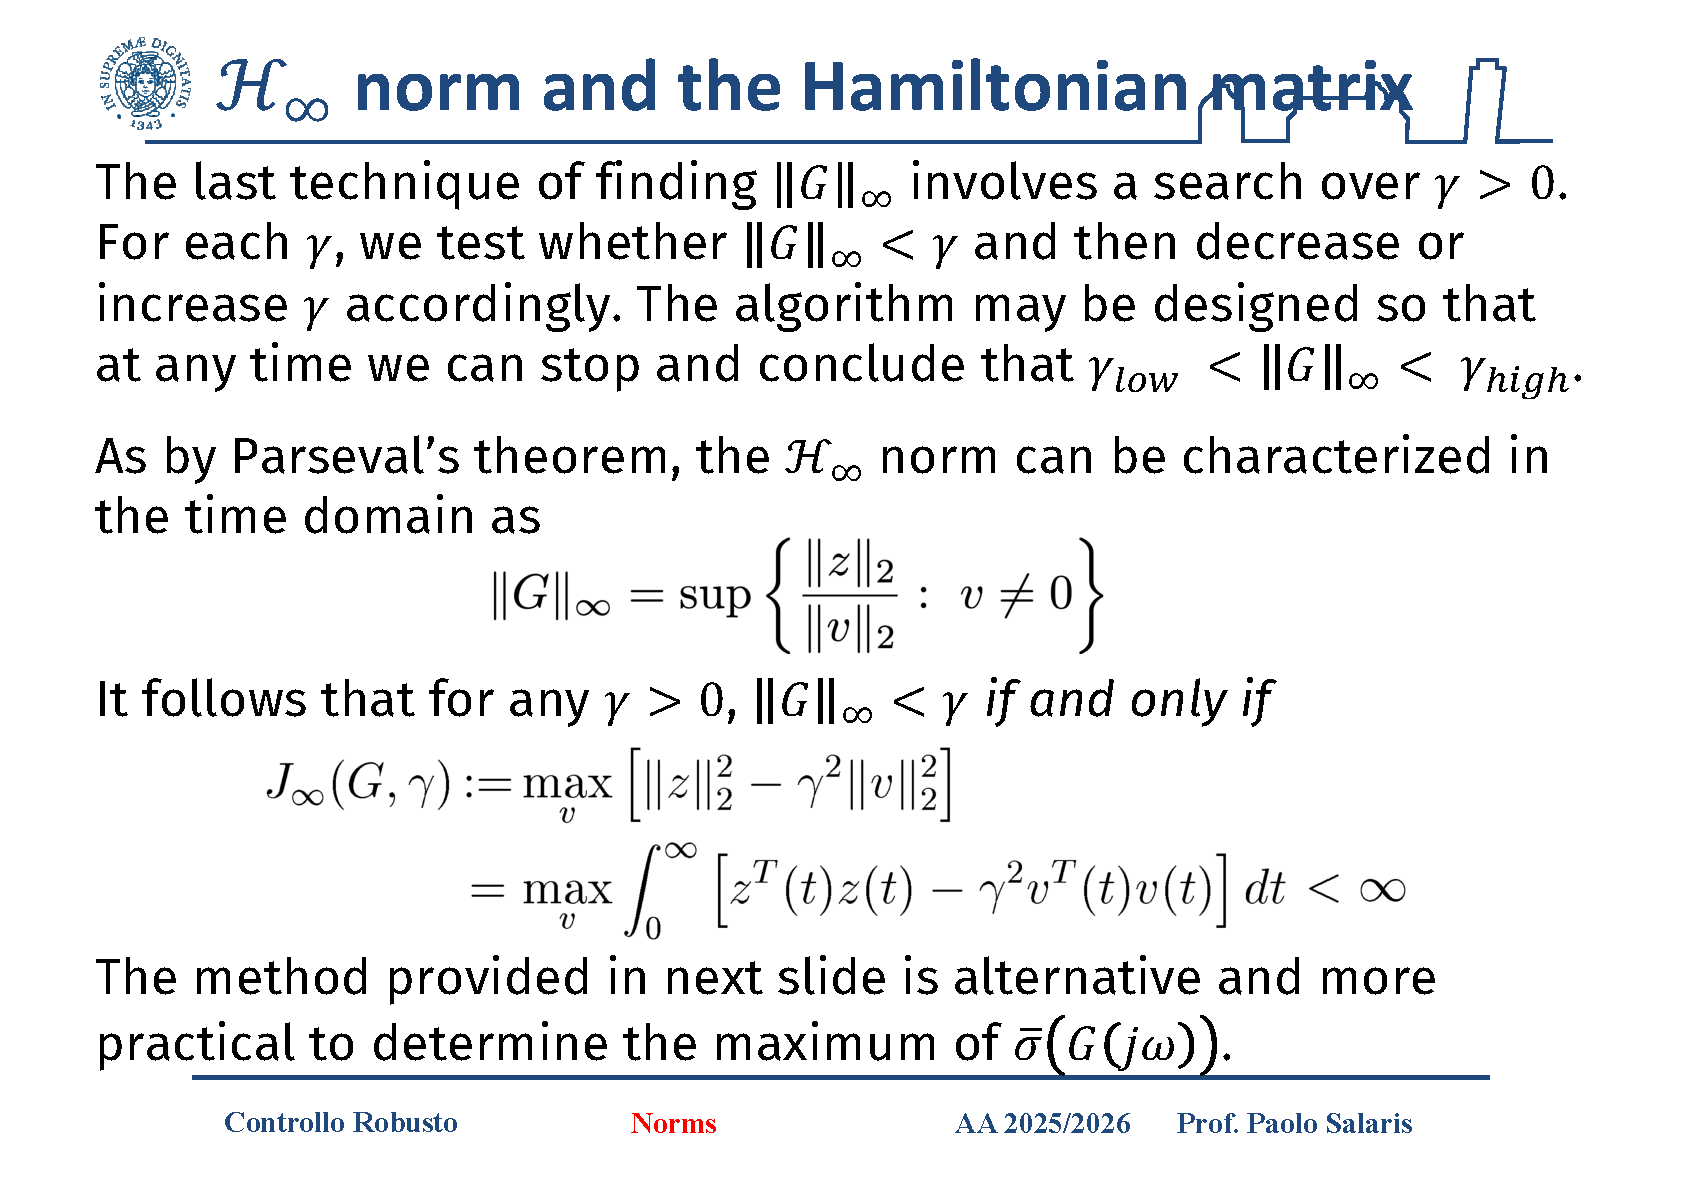
\includegraphics[width=\linewidth]{images8/norms-new-33-53-009.png}
        \caption{Riformulazione del problema come test di appartenenza alla soglia $\gamma$.}
    \end{subfigure}
    \caption{Il modo pratico di calcolare $\|G\|_{H_\infty}$ consiste nel testare iterativamente se il guadagno massimo resta sotto una soglia assegnata.}
\end{figure}

\subsection{Il test con la matrice Hamiltoniana}

\subsubsection{Dalla soglia \texorpdfstring{$\gamma$}{gamma} alla funzione \texorpdfstring{$Q(s)$}{Q(s)}}

La slide 42 anticipa l'intera pipeline. Per calcolare la norma $H_\infty$ non si cerca direttamente il massimo di $\bar{\sigma}(G(j\omega))$; si fissa una soglia $\gamma$ e si testa se il sistema resta sempre sotto tale soglia. Il risultato attribuito nelle slide a Doyle et al. dice che, per un sistema stabile, la condizione
$$
\|G\|_{H_\infty}<\gamma
$$
pu\`o essere ricondotta alla funzione
$$
Q(s)=I-\frac{1}{\gamma^2}G^T(-s)G(s).
$$
L'idea \`e: se $\gamma$ \`e pi\`u grande del massimo guadagno del sistema, allora $Q(j\omega)$ deve restare positiva per ogni frequenza; se invece il grafico dei valori singolari tocca o supera $\gamma$, da qualche parte $Q(j\omega)$ perde positivit\`a.

Le slide 43 e 44 esplicitano questo passaggio. Per definizione,
$$
\|G\|_{H_\infty}
=
\sup_{\omega\in\mathbb{R}}\bar{\sigma}\!\bigl(G(j\omega)\bigr).
$$
Quindi
$$
\|G\|_{H_\infty}<\gamma
\quad\Longleftrightarrow\quad
\bar{\sigma}\!\bigl(G(j\omega)\bigr)<\gamma
\qquad
\forall\,\omega\in\mathbb{R}.
$$
Per sistemi reali, sull'asse immaginario vale
$$
\bar{\sigma}\!\bigl(G(j\omega)\bigr)
=
\sqrt{\lambda_{\max}\!\bigl(G^T(-j\omega)G(j\omega)\bigr)}.
$$
Qui $G^T(-j\omega)$ \`e il modo usato nelle slide per scrivere l'aggiunto frequenziale: nel caso reale coincide con il complesso coniugato trasposto di $G(j\omega)$.

La disuguaglianza sui valori singolari diventa allora
$$
\lambda_{\max}\!\bigl(G^T(-j\omega)G(j\omega)\bigr)<\gamma^2.
$$
Ora entra un fatto elementare di algebra lineare: per una matrice hermitiana $M$,
$$
\lambda_{\max}(M)<c
\quad\Longleftrightarrow\quad
cI-M>0.
$$
Infatti gli autovalori di $cI-M$ sono $c-\lambda_i(M)$, tutti positivi se e solo se ogni $\lambda_i(M)$ \`e minore di $c$. Applicandolo a
$$
M=G^T(-j\omega)G(j\omega),
\qquad c=\gamma^2,
$$
si ottiene
$$
\gamma^2I-G^T(-j\omega)G(j\omega)>0.
$$
Dividendo per $\gamma^2$ si ottiene esattamente la matrice delle slide:
$$
Q(j\omega)
=
I-\frac{1}{\gamma^2}G^T(-j\omega)G(j\omega),
$$
per cui
$$
\|G\|_{H_\infty}<\gamma
\qquad\Longleftrightarrow\qquad
Q(j\omega)>0
\quad
\forall\,\omega\in\mathbb{R}.
$$

\begin{figure}[H]
    \centering
    \begin{subfigure}{0.48\textwidth}
        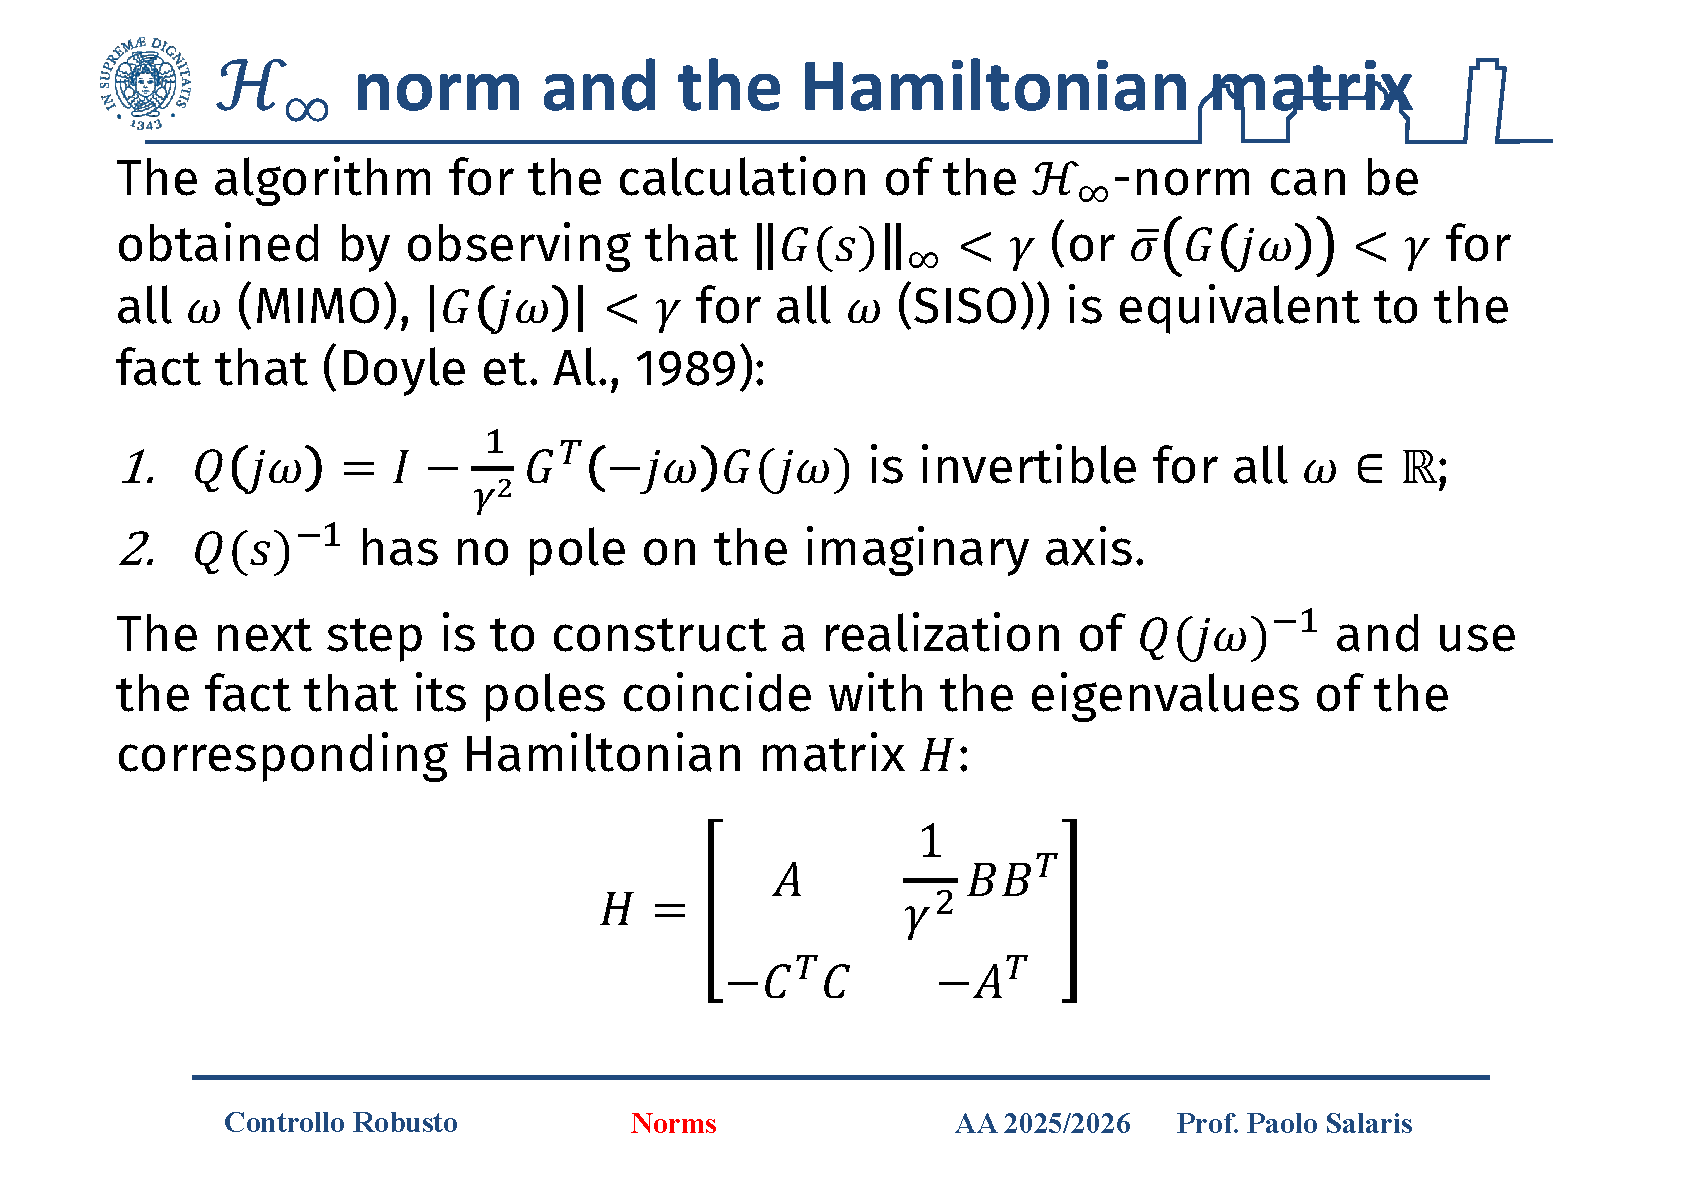
\includegraphics[width=\linewidth]{images8/norms-new-33-53-010.png}
        \caption{Impostazione del test $\|G\|_{H_\infty}<\gamma$ e introduzione della funzione $Q(s)$.}
    \end{subfigure}
    \hfill
    \begin{subfigure}{0.48\textwidth}
        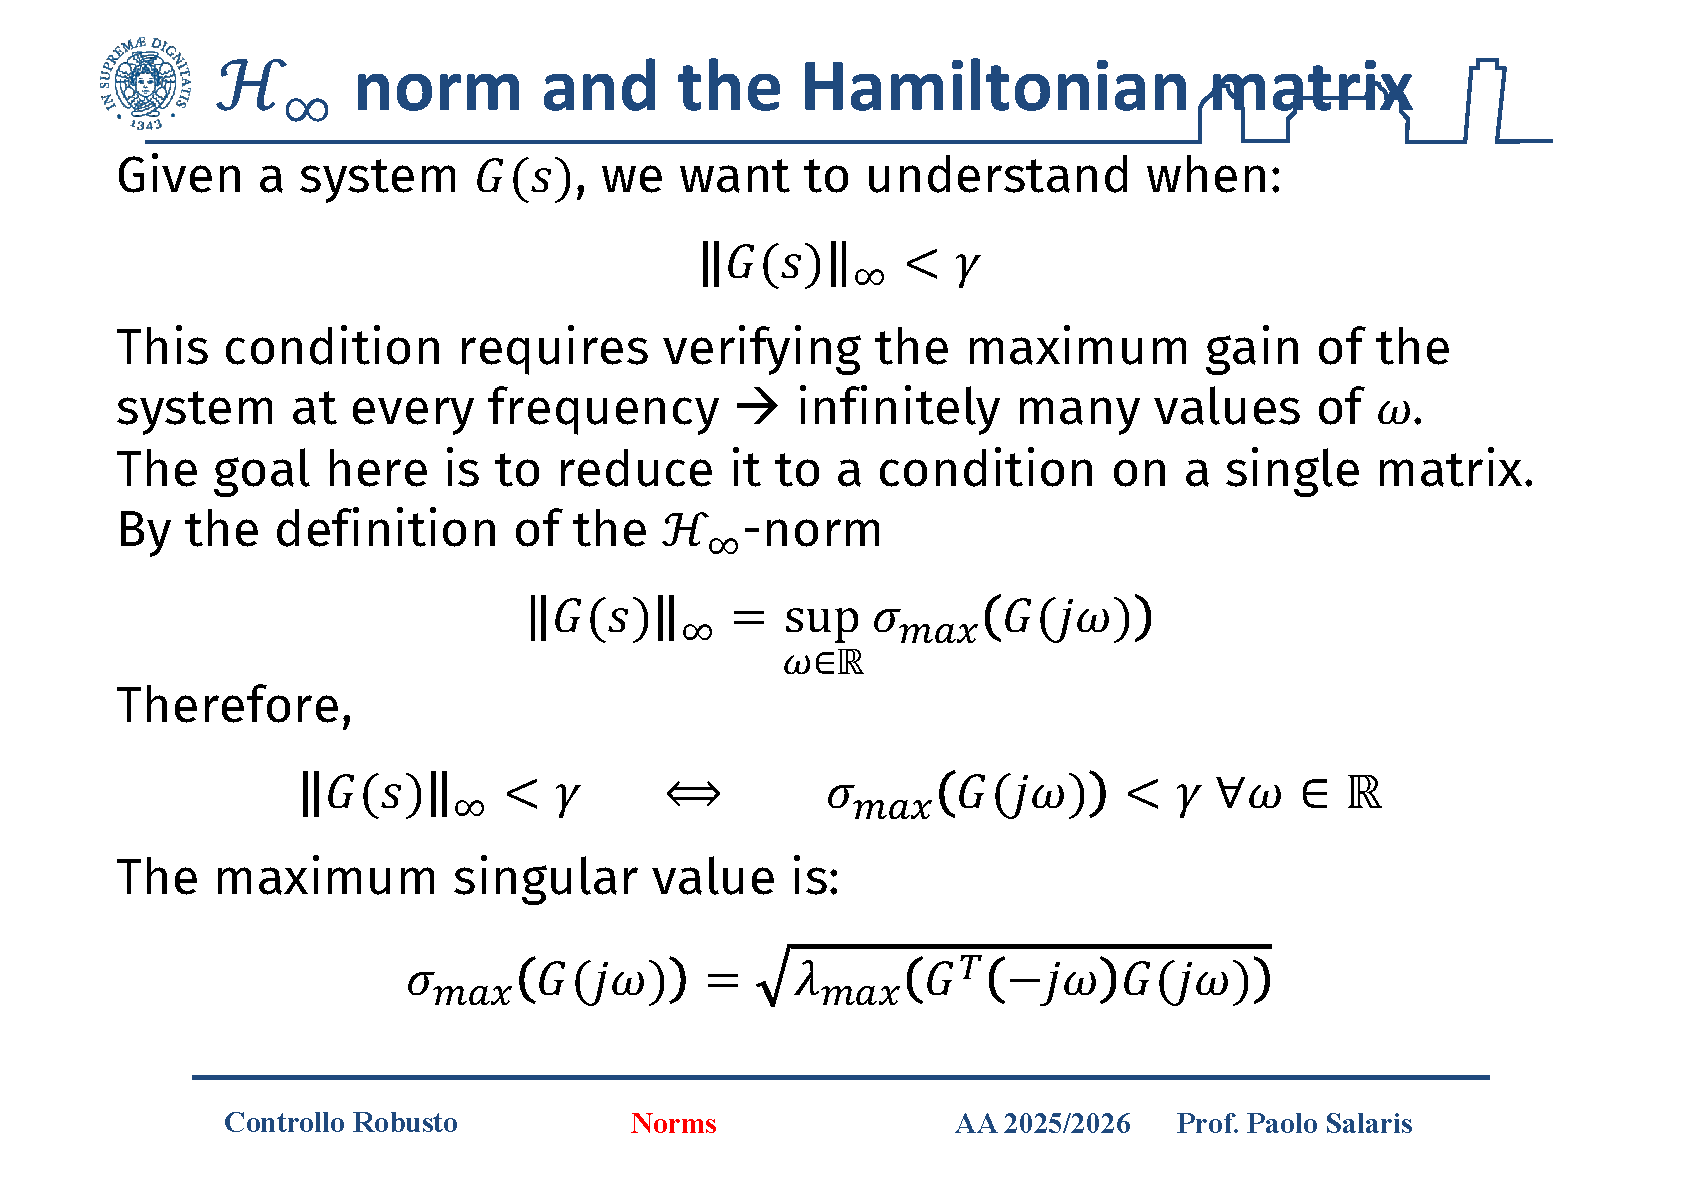
\includegraphics[width=\linewidth]{images8/norms-new-33-53-011.png}
        \caption{Riduzione del controllo su infinite frequenze a una condizione sul massimo valore singolare.}
    \end{subfigure}
    \caption{Le nuove slide rendono esplicito il passaggio dalla norma $H_\infty$ al confronto frequenziale con la soglia $\gamma$.}
\end{figure}

\begin{figure}[H]
    \centering
    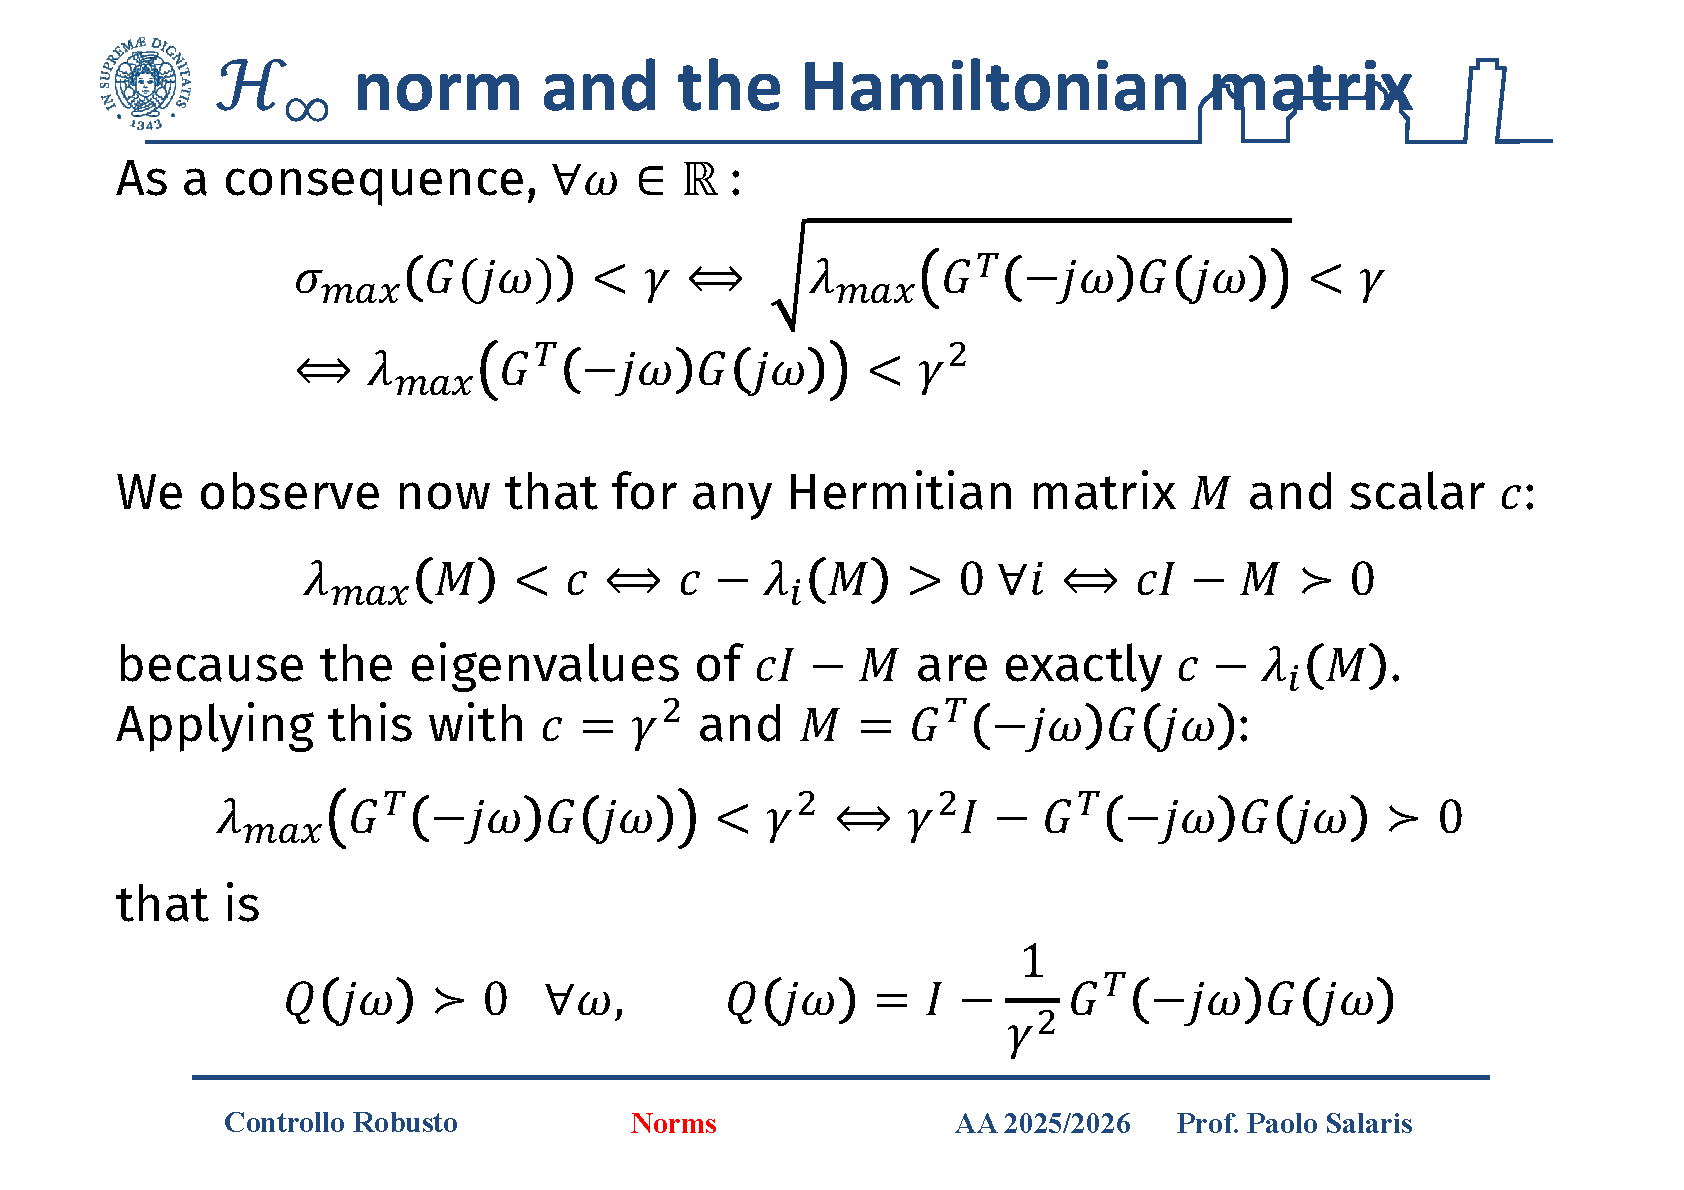
\includegraphics[width=0.82\textwidth]{images8/norms-new-33-53-012.png}
    \caption{La condizione sul massimo valore singolare viene trasformata nella positivit\`a definita della matrice $Q(j\omega)$.}
\end{figure}

\subsubsection{Da positivit\`a a invertibilit\`a}

Le slide 45 e 46 fanno un passaggio che a prima vista pu\`o sembrare minore, ma \`e il punto che permette di abbandonare la disuguaglianza matriciale. Abbiamo ottenuto
$$
Q(j\omega)>0\qquad\forall \omega.
$$
Una matrice positiva definita ha tutti gli autovalori positivi, quindi determinante non nullo, quindi \`e invertibile. Dunque
$$
Q(j\omega)>0\ \forall\omega
\quad\Longrightarrow\quad
Q(j\omega)\ \text{invertibile}\ \forall\omega.
$$

La direzione opposta richiede la piccola argomentazione di continuit\`a mostrata nella slide 46. Poich\'e $Q(j\omega)$ \`e hermitiana, i suoi autovalori sono reali. Consideriamo l'autovalore minimo
$$
\lambda_{\min}\!\bigl(Q(j\omega)\bigr).
$$
Al variare di $\omega$, questa quantit\`a \`e continua. Se $Q(j\omega)$ \`e invertibile per ogni $\omega$, nessun autovalore pu\`o annullarsi. Se inoltre $Q(j\omega)$ \`e positiva per frequenze molto alte, allora $\lambda_{\min}$ parte positiva e non pu\`o diventare negativa senza attraversare lo zero. Ma lo zero \`e escluso dall'invertibilit\`a. Quindi, sotto la condizione corretta all'infinito, l'invertibilit\`a per ogni $\omega$ equivale alla positivit\`a per ogni $\omega$.

La slide 47 distingue proprio la condizione all'infinito. Se $G$ \`e strettamente propria,
$$
G(s)=C(sI-A)^{-1}B,
\qquad D=0,
$$
si ha
$$
G(j\infty)=0,
\qquad
Q(j\infty)=I>0.
$$
Quindi la positivit\`a ad alta frequenza \`e automatica. Se invece $G$ \`e propria ma non strettamente propria,
$$
G(s)=C(sI-A)^{-1}B+D,
$$
allora
$$
G(j\infty)=D,
\qquad
Q(j\infty)=I-\frac{1}{\gamma^2}D^TD.
$$
Questa matrice \`e positiva definita se e solo se
$$
\bar{\sigma}(D)<\gamma.
$$
La slide dice giustamente che questa condizione va verificata separatamente: se fallisce, la soglia $\gamma$ \`e gi\`a violata alla frequenza infinita e il test si ferma.

\begin{figure}[H]
    \centering
    \begin{subfigure}{0.48\textwidth}
        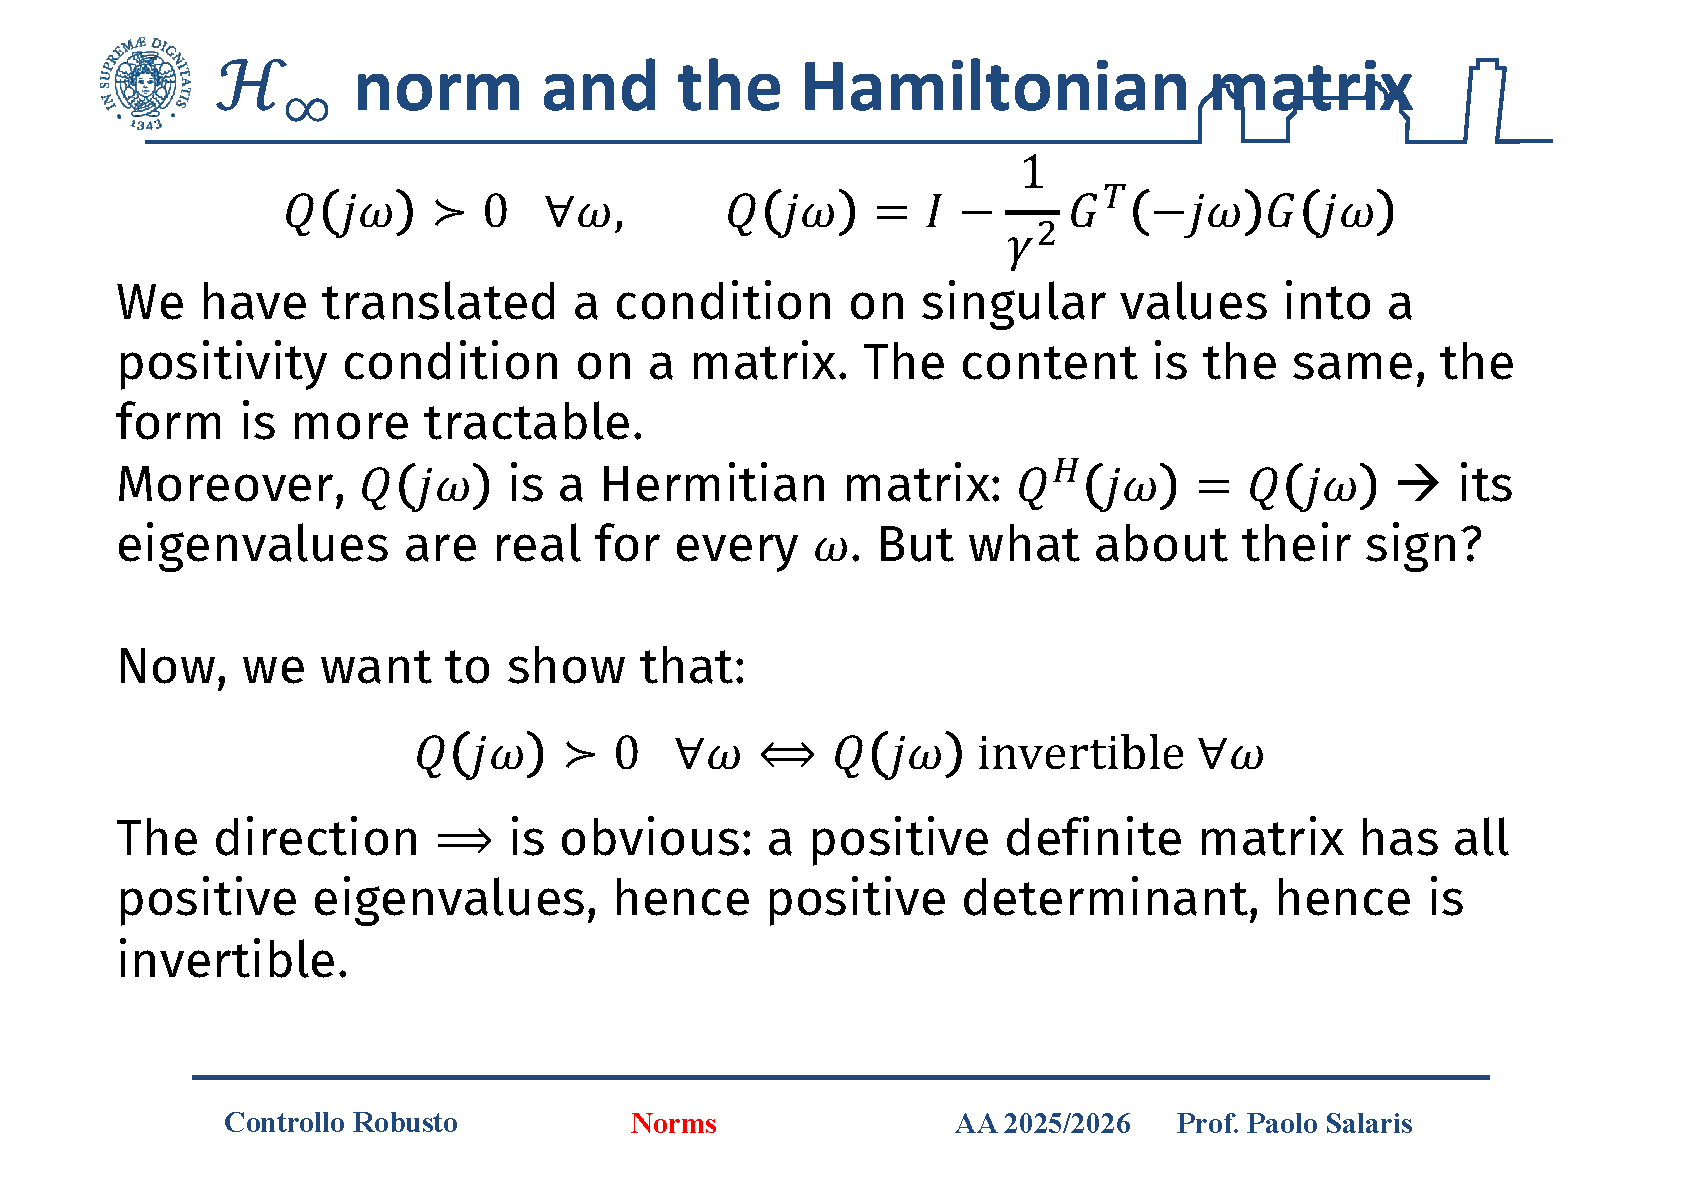
\includegraphics[width=\linewidth]{images8/norms-new-33-53-013.png}
        \caption{Prima direzione: la positivit\`a di $Q(j\omega)$ implica invertibilit\`a.}
    \end{subfigure}
    \hfill
    \begin{subfigure}{0.48\textwidth}
        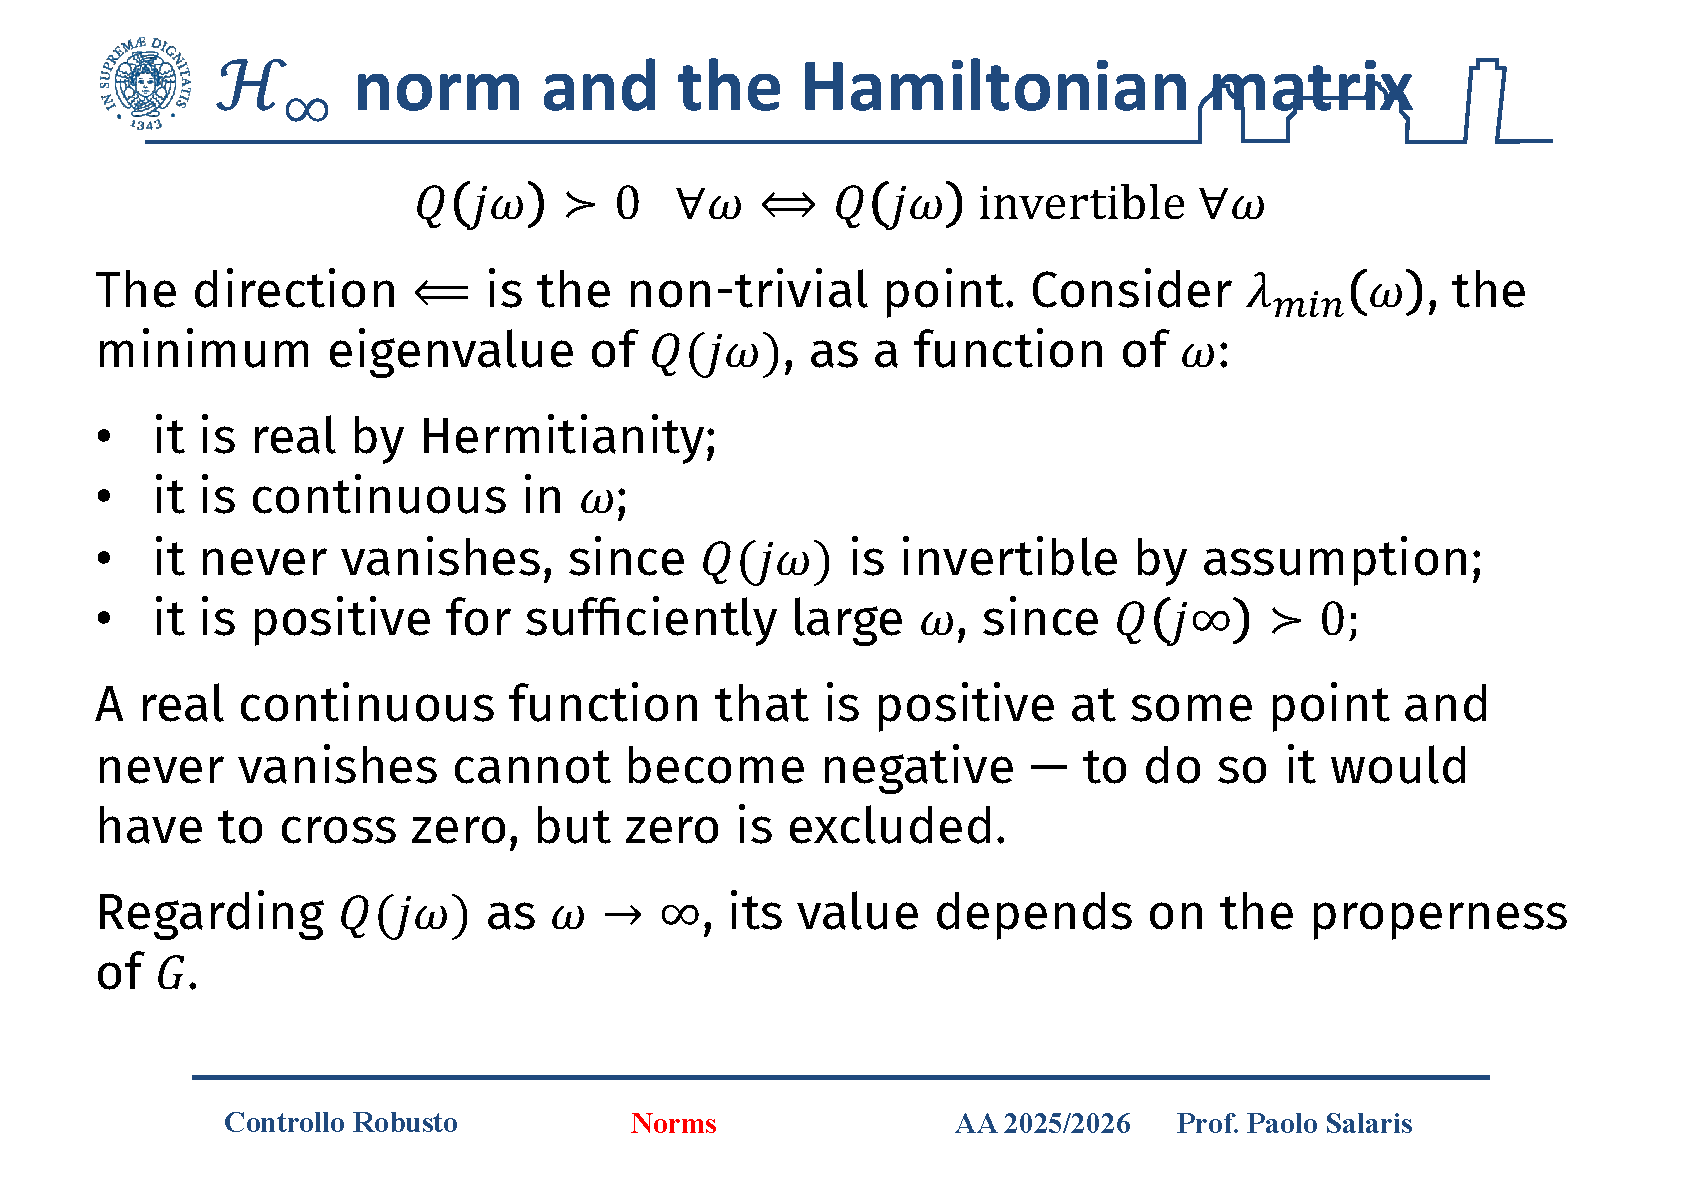
\includegraphics[width=\linewidth]{images8/norms-new-33-53-014.png}
        \caption{Seconda direzione: continuit\`a dell'autovalore minimo e impossibilit\`a di attraversare lo zero.}
    \end{subfigure}
    \caption{La positivit\`a di $Q(j\omega)$ viene ricondotta all'invertibilit\`a su tutto l'asse immaginario pi\`u una condizione all'infinito.}
\end{figure}

\begin{figure}[H]
    \centering
    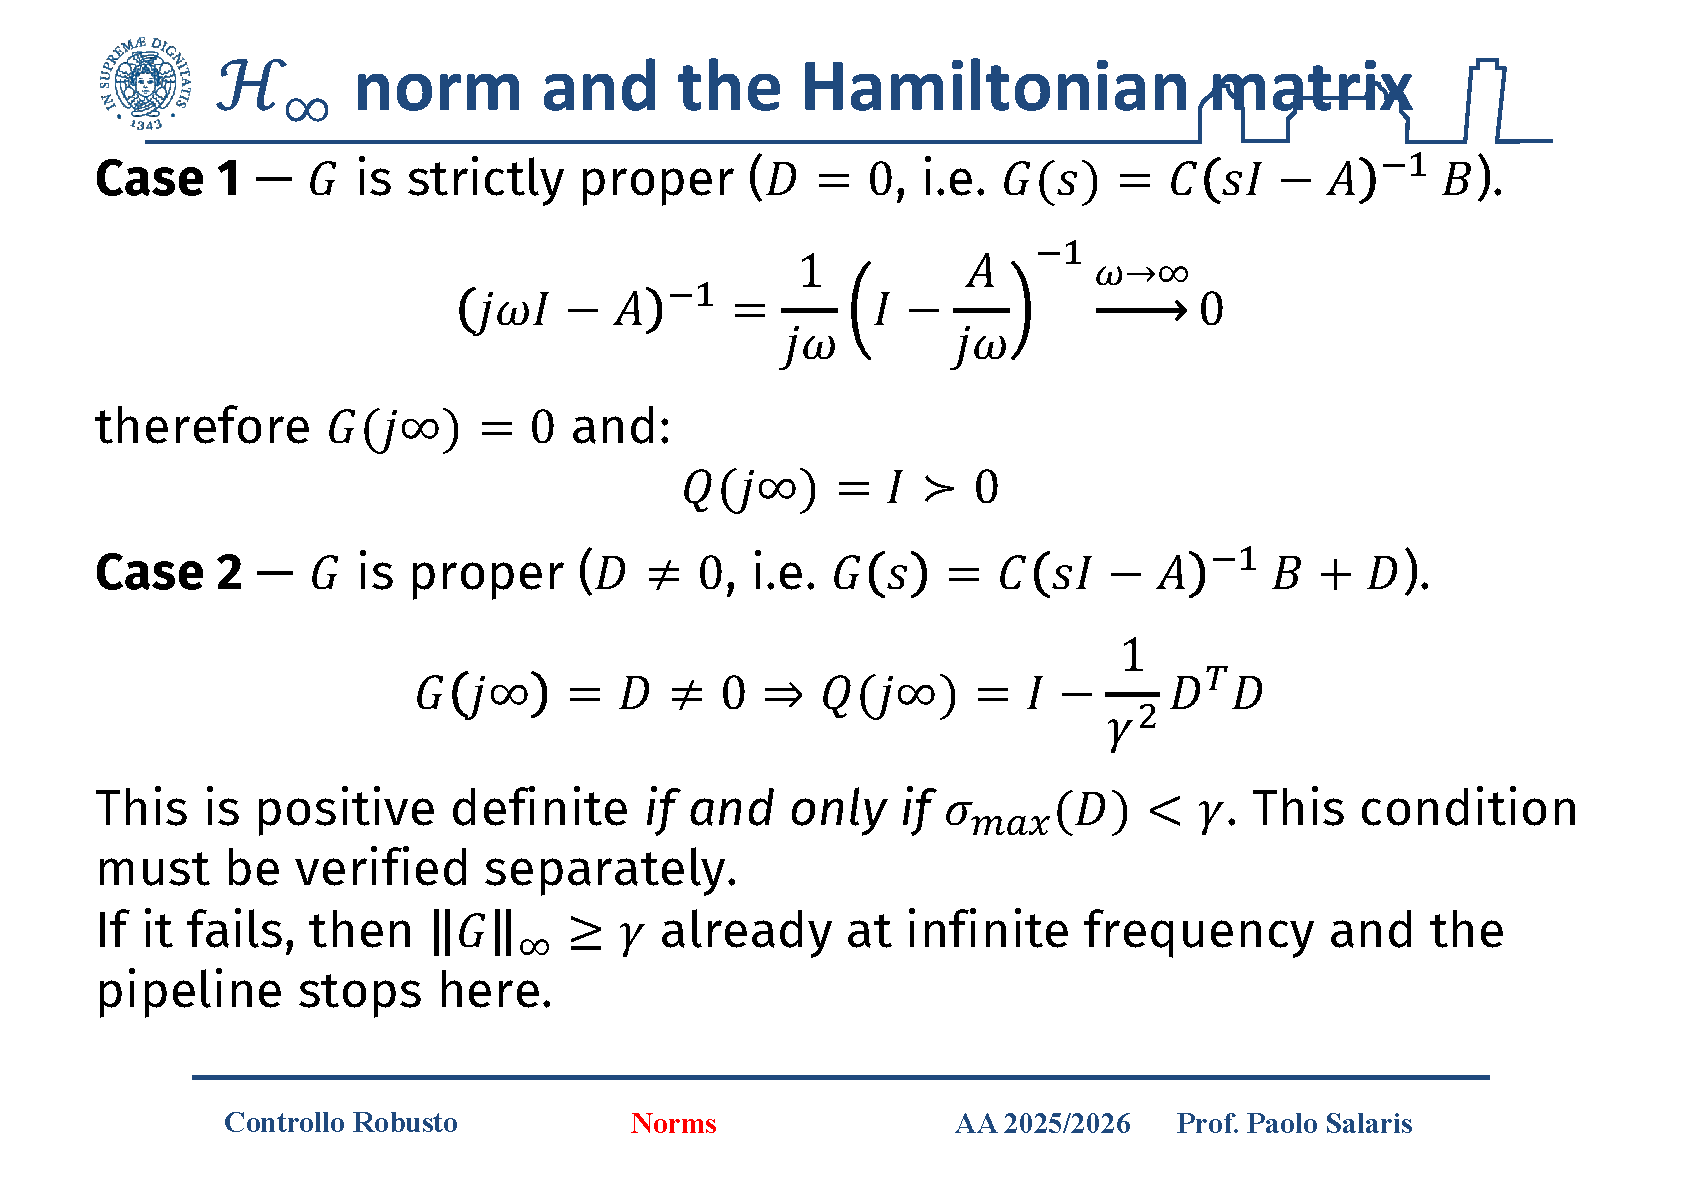
\includegraphics[width=0.82\textwidth]{images8/norms-new-33-53-015.png}
    \caption{La condizione all'infinito \`e automatica per sistemi strettamente propri, mentre per sistemi propri richiede $\bar{\sigma}(D)<\gamma$.}
\end{figure}

\subsubsection{Da invertibilit\`a ad assenza di poli sull'asse immaginario}

La slide 48 traduce l'invertibilit\`a frequenziale in una frase sui poli. Poich\'e $Q(s)$ \`e una matrice razionale, $Q^{-1}(s)$ ha poli nei punti in cui $Q(s)$ perde rango, cio\`e dove
$$
\det Q(s)=0.
$$
Sull'asse immaginario poniamo $s=j\omega$, quindi
$$
Q(j\omega)\ \text{invertibile per ogni }\omega
\qquad\Longleftrightarrow\qquad
Q^{-1}(s)\ \text{non ha poli su }j\mathbb{R}.
$$

Nel caso strettamente proprio, o nel caso proprio dopo aver verificato $\bar{\sigma}(D)<\gamma$, la catena logica costruita fin qui \`e:
$$
\|G\|_{H_\infty}<\gamma
\Longleftrightarrow
Q(j\omega)>0\ \forall\omega
\Longleftrightarrow
Q(j\omega)\ \text{invertibile}\ \forall\omega
\Longleftrightarrow
Q^{-1}(s)\ \text{senza poli su }j\mathbb{R}.
$$
Questo \`e il punto esatto in cui la lezione cambia linguaggio. Non stiamo pi\`u cercando il massimo di una curva frequenziale; stiamo cercando i poli di una funzione razionale. Se costruiamo una realizzazione di $Q^{-1}(s)$, quei poli saranno autovalori della matrice dinamica della realizzazione.

\begin{figure}[H]
    \centering
    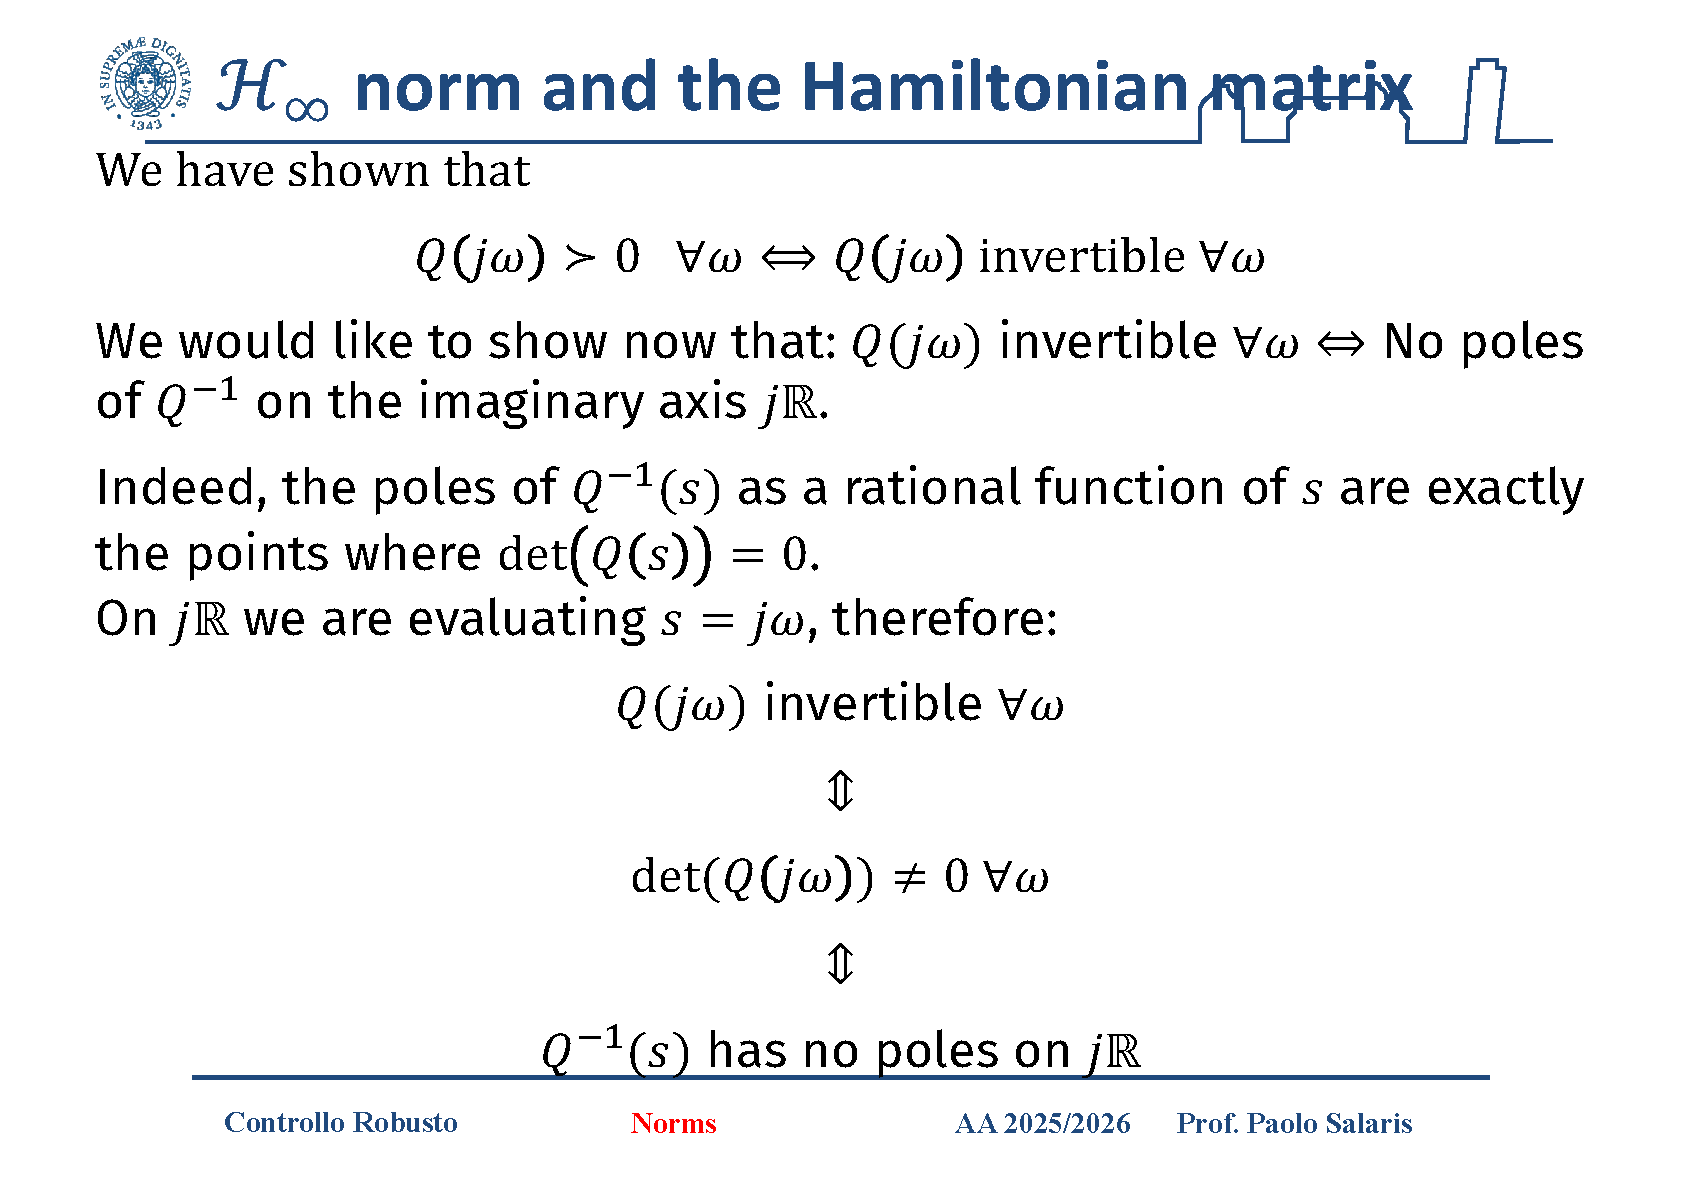
\includegraphics[width=0.82\textwidth]{images8/norms-new-33-53-016.png}
    \caption{L'invertibilit\`a di $Q(j\omega)$ per ogni frequenza equivale all'assenza di poli di $Q^{-1}(s)$ sull'asse immaginario.}
\end{figure}

\begin{focusbox}
\textbf{Perch\'e questo passaggio \`e utile.} Il controllo robusto lavora spesso con vincoli validi per ogni frequenza. La costruzione di $Q^{-1}$ trasforma un vincolo infinito in un controllo spettrale: esistono o no autovalori su $j\mathbb{R}$?
\end{focusbox}

\subsubsection{Comparsa della matrice Hamiltoniana}

La slide 49 mostra il passo finale della costruzione. Per semplicit\`a si assume prima il caso strettamente proprio
$$
G(s)=C(sI-A)^{-1}B,
\qquad D=0.
$$
Allora una realizzazione di $Q^{-1}(s)$ ha come matrice dinamica
$$
\mathcal{H}_\gamma
=
\begin{bmatrix}
A & \gamma^{-2}BB^T\\
-C^TC & -A^T
\end{bmatrix}.
$$
La formula scritta nelle slide si pu\`o leggere come
$$
Q^{-1}(s)
=
I+
\frac{1}{\gamma^2}
\begin{bmatrix}0 & B^T\end{bmatrix}
(sI-\mathcal{H}_\gamma)^{-1}
\begin{bmatrix}B\\0\end{bmatrix}.
$$
Poich\'e i poli della funzione di trasferimento realizzata sono contenuti negli autovalori della matrice dinamica, il test diventa:
$$
Q^{-1}(s)\ \text{senza poli su }j\mathbb{R}
\quad\Longleftrightarrow\quad
\mathcal{H}_\gamma\ \text{senza autovalori su }j\mathbb{R},
$$
al netto di eventuali cancellazioni non patologiche nella realizzazione.

Il criterio pratico coerente con le slide \`e quindi:
\begin{enumerate}
    \item si fissa una soglia $\gamma$;
    \item se $D\neq0$, si controlla prima $\bar{\sigma}(D)<\gamma$;
    \item si costruisce la Hamiltoniana $\mathcal{H}_\gamma$;
    \item si verifica se $\mathcal{H}_\gamma$ ha autovalori sull'asse immaginario.
\end{enumerate}
Se compaiono autovalori su $j\mathbb{R}$, la soglia $\gamma$ \`e stata raggiunta da qualche valore singolare del sistema. Se non compaiono e la condizione all'infinito \`e soddisfatta, la soglia \`e compatibile con $\|G\|_{H_\infty}<\gamma$.

La bisezione su $\gamma$ nasce da qui: invece di massimizzare direttamente $\bar{\sigma}(G(j\omega))$, si restringe progressivamente l'intervallo delle soglie ammissibili testando la Hamiltoniana.

\begin{figure}[H]
    \centering
    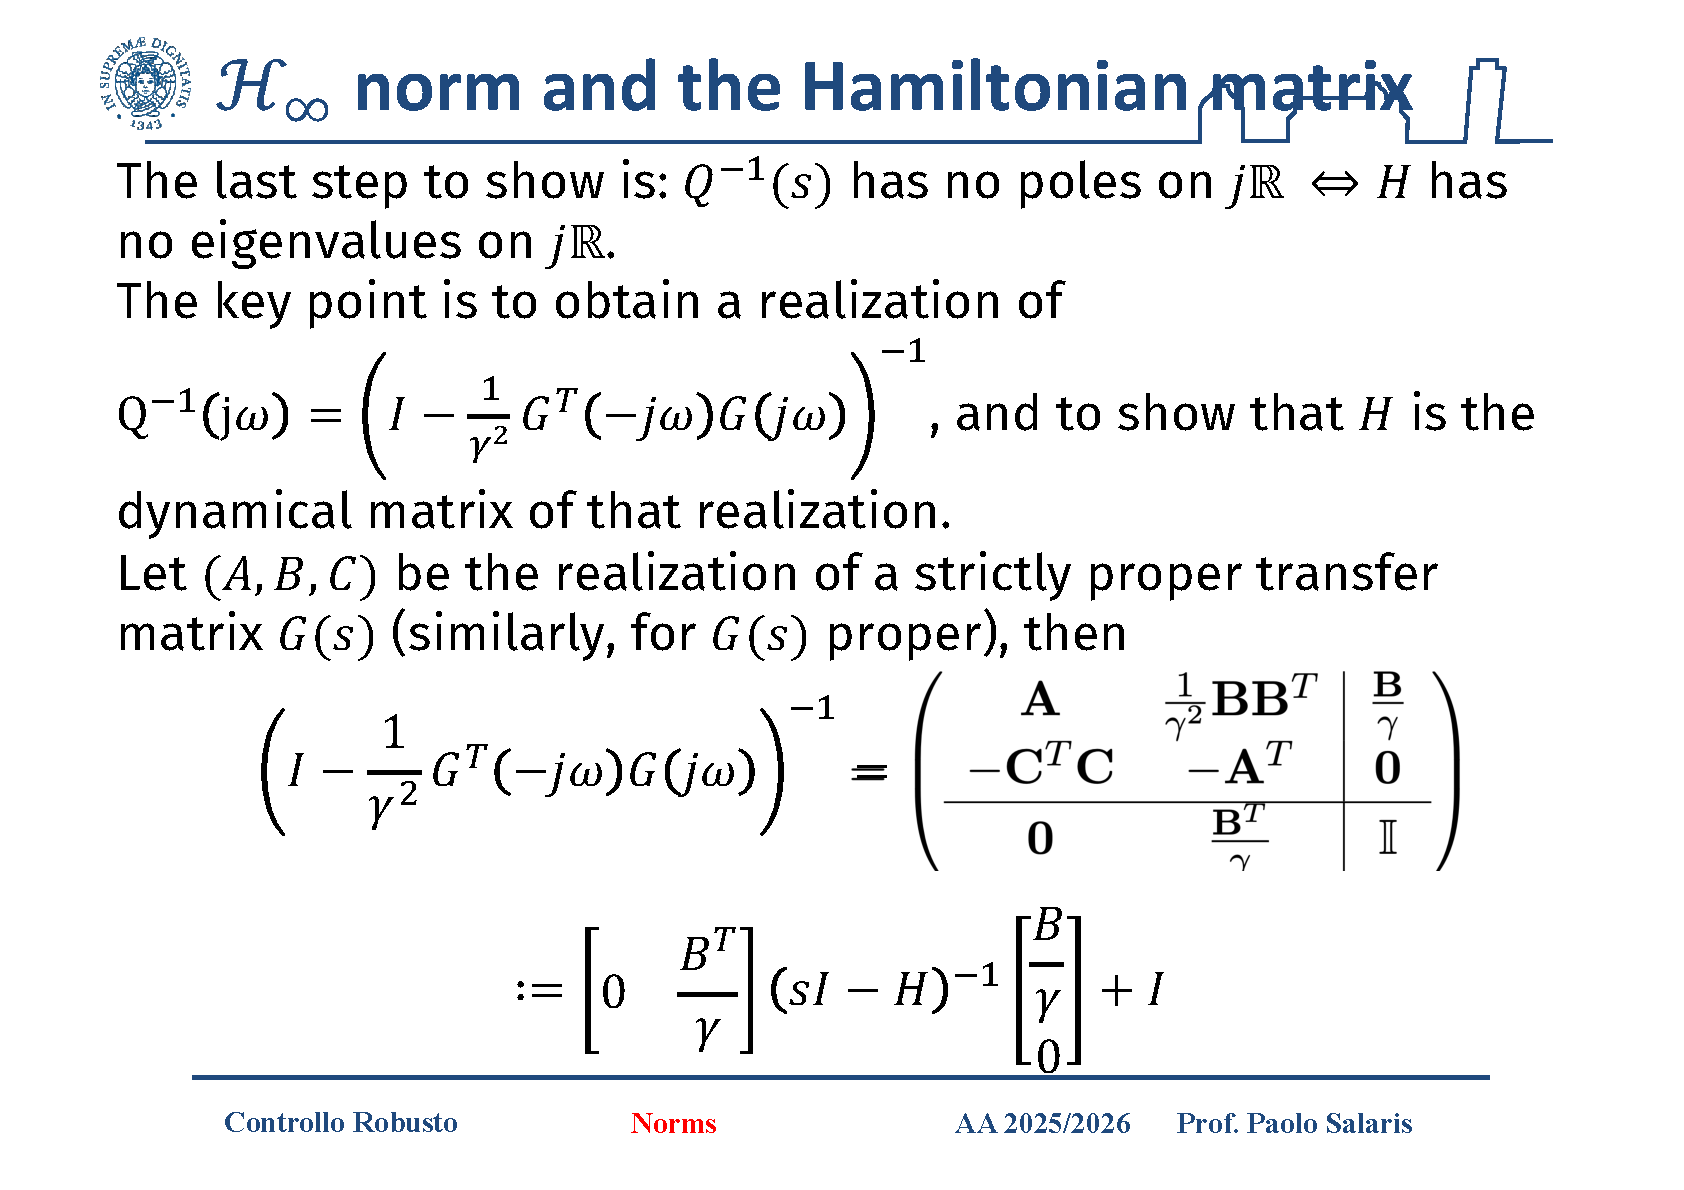
\includegraphics[width=0.82\textwidth]{images8/norms-new-33-53-017.png}
    \caption{La realizzazione di $Q(s)^{-1}$ porta alla matrice Hamiltoniana associata alla soglia $\gamma$.}
\end{figure}

\subsubsection{Perch\'e compare \texorpdfstring{$G^T(-s)$}{G trasposto(-s)}}

Le slide 50 e 51 non si limitano a dare la Hamiltoniana: mostrano da dove arriva. Partiamo da
$$
G(s)=C(sI-A)^{-1}B,
$$
e calcoliamo la funzione riflessa che compare in $Q(s)$:
$$
G^T(-s)=-B^T(sI+A^T)^{-1}C^T.
$$
Quindi $G^T(-s)$ si realizza con matrice dinamica $-A^T$, ingresso attraverso $-C^T$ e uscita attraverso $B^T$. Questo spiega il blocco $-A^T$ nella Hamiltoniana.

La relazione chiusa della slide \`e
$$
e(s)=r(s)+\frac{1}{\gamma^2}G^T(-s)G(s)e(s).
$$
Portando il termine in $e$ a sinistra,
$$
e(s)
=
\left(I-\frac{1}{\gamma^2}G^T(-s)G(s)\right)^{-1}r(s).
$$
Questa \`e proprio la funzione $Q^{-1}(s)$ applicata al segnale $r$.

Scriviamo ora i due sottosistemi. Il primo, associato a $G(s)$, prende $e$ in ingresso:
$$
\dot x_1=Ax_1+Be,
\qquad
u=Cx_1.
$$
Il secondo, associato a $G^T(-s)$, prende $u$ in ingresso:
$$
\dot x_2=-A^Tx_2-C^Tu,
\qquad
y=B^Tx_2.
$$
La chiusura della slide \`e
$$
e=r+\frac{1}{\gamma^2}y
=r+\frac{1}{\gamma^2}B^Tx_2.
$$
Sostituendo $e$ nella dinamica di $x_1$ e $u=Cx_1$ nella dinamica di $x_2$, si ottiene
$$
\begin{bmatrix}
\dot x_1\\
\dot x_2
\end{bmatrix}
=
\begin{bmatrix}
A & \gamma^{-2}BB^T\\
-C^TC & -A^T
\end{bmatrix}
\begin{bmatrix}
x_1\\
x_2
\end{bmatrix}
+
\begin{bmatrix}
B\\
0
\end{bmatrix}r.
$$
La matrice dinamica dell'interconnessione \`e quindi esattamente
$$
\mathcal{H}_\gamma
=
\begin{bmatrix}
A & \gamma^{-2}BB^T\\
-C^TC & -A^T
\end{bmatrix}.
$$

La slide 52 riscrive la stessa realizzazione nel dominio della frequenza:
$$
e(s)
=
\left[
I+
\frac{1}{\gamma^2}
\begin{bmatrix}0 & B^T\end{bmatrix}
(sI-\mathcal{H}_\gamma)^{-1}
\begin{bmatrix}B\\0\end{bmatrix}
\right]r(s).
$$
Questo conferma che i poli di $Q^{-1}(s)$ sono governati dagli autovalori di $\mathcal{H}_\gamma$.

La slide 53 chiude il cerchio con la forma determinantalmente equivalente:
$$
\det\!\left(I-\frac{1}{\gamma^2}G^T(-s)G(s)\right)=0
\qquad\Longleftrightarrow\qquad
\det\!\bigl(\gamma^2I-G^T(-s)G(s)\bigr)=0.
$$
Questi sono i punti complessi in cui la soglia $\gamma$ viene toccata. Se uno di questi punti cade su $s=j\omega$, allora per quella frequenza un valore singolare di $G(j\omega)$ vale $\gamma$; corrispondentemente, la Hamiltoniana mostra un autovalore sull'asse immaginario.

La catena completa delle slide \`e dunque:
\begin{itemize}
    \item $\|G\|_{H_\infty}<\gamma$ impone $\bar{\sigma}(G(j\omega))<\gamma$ per ogni frequenza;
    \item questa condizione equivale a $Q(j\omega)>0$;
    \item la positivit\`a di $Q(j\omega)$ equivale, con la corretta condizione all'infinito, all'invertibilit\`a di $Q(j\omega)$;
    \item l'invertibilit\`a su $j\mathbb{R}$ equivale all'assenza di poli di $Q^{-1}(s)$ su $j\mathbb{R}$;
    \item una realizzazione di $Q^{-1}(s)$ ha matrice dinamica $\mathcal{H}_\gamma$.
\end{itemize}
Questo \`e il ponte costruito dalla lezione: una disuguaglianza frequenziale per tutte le $\omega$ viene trasformata in un test sugli autovalori di una matrice finita.

\begin{figure}[H]
    \centering
    \begin{subfigure}{0.48\textwidth}
        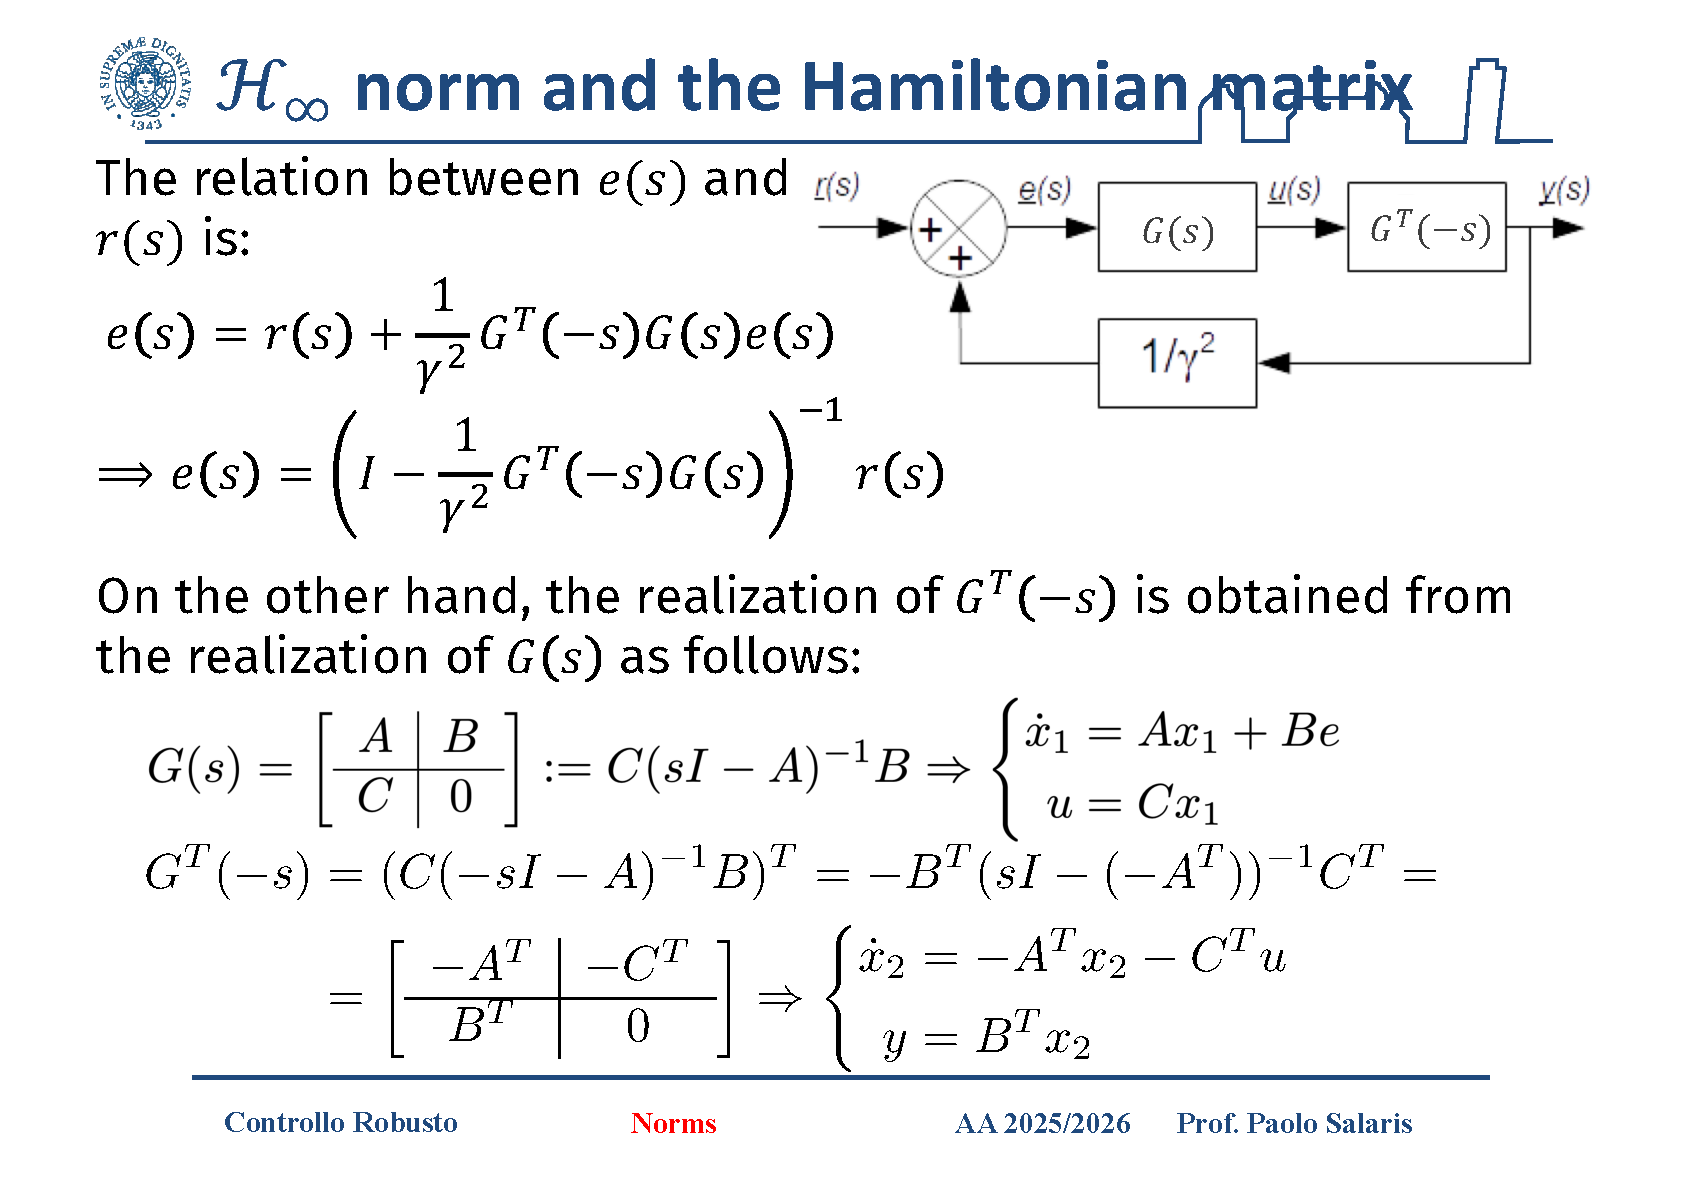
\includegraphics[width=\linewidth]{images8/norms-new-33-53-018.png}
        \caption{Relazione chiusa fra $r$, $e$, $G(s)$ e $G^T(-s)$ nella costruzione di $Q^{-1}(s)$.}
    \end{subfigure}
    \hfill
    \begin{subfigure}{0.48\textwidth}
        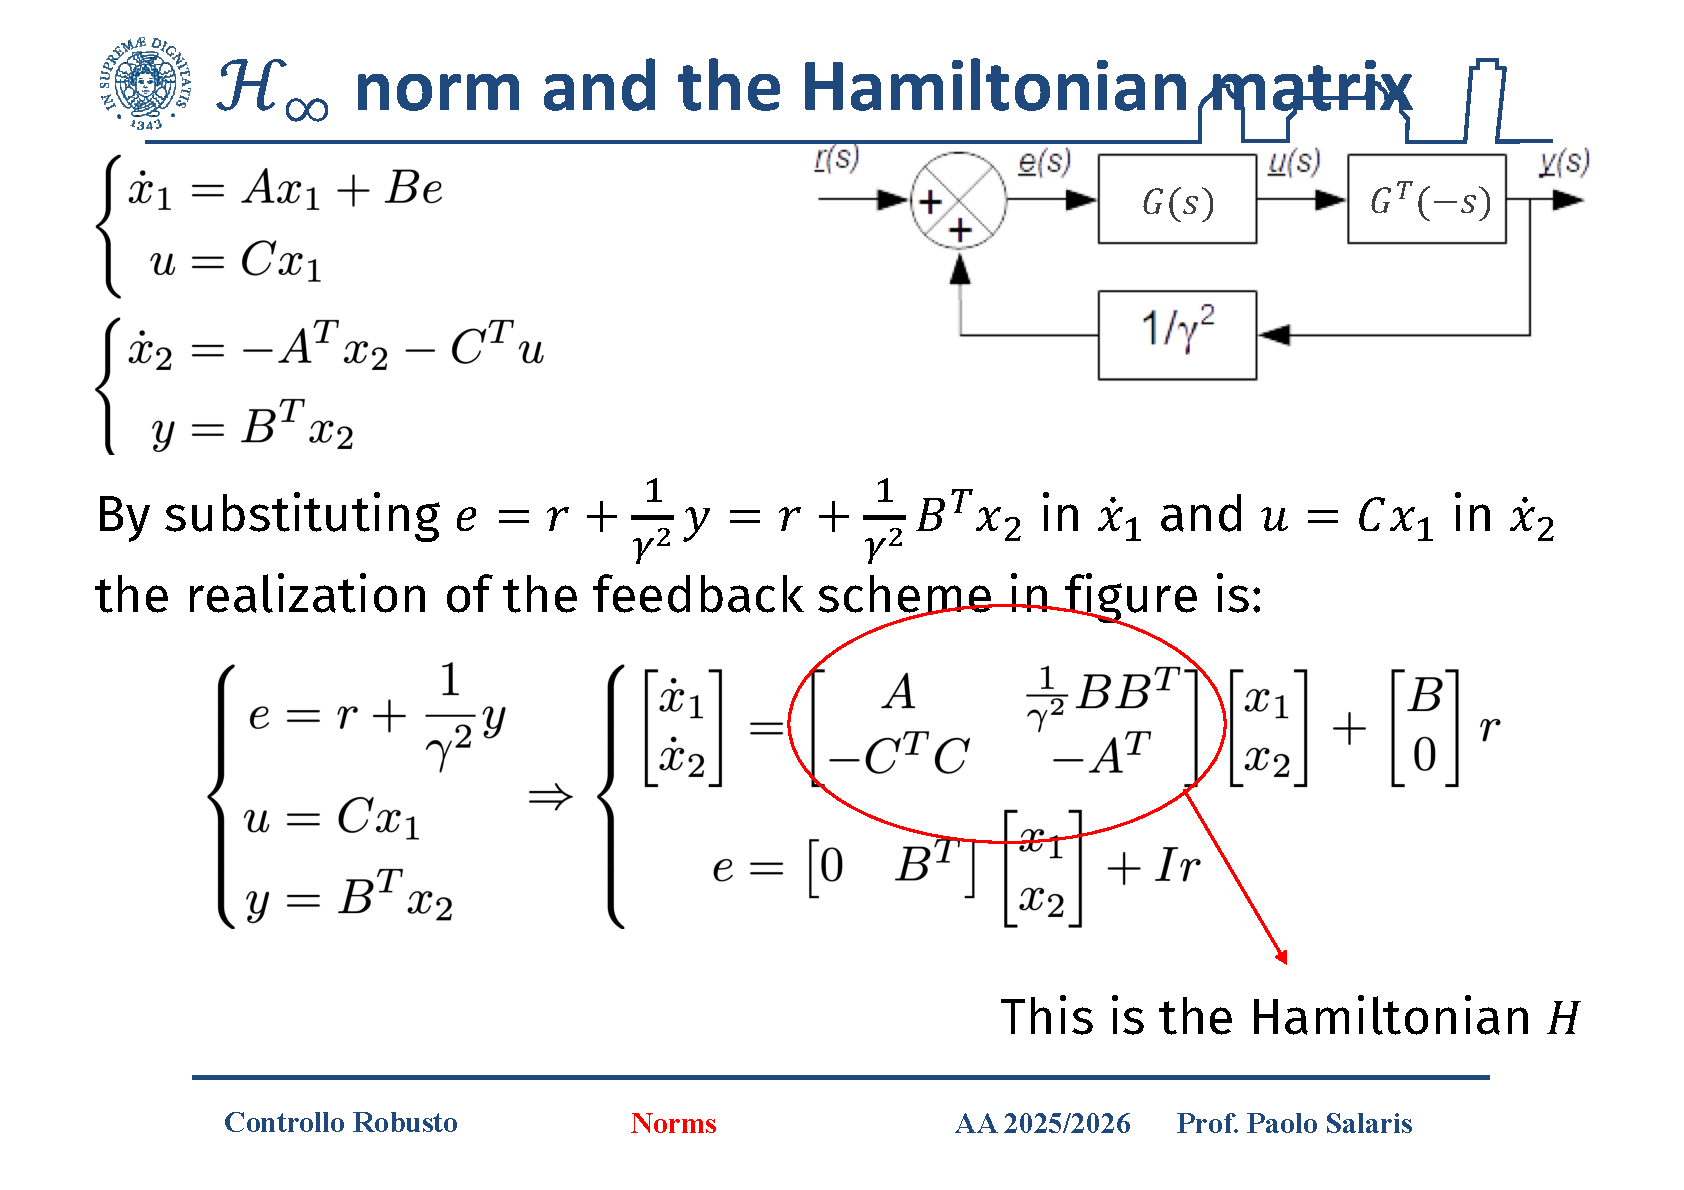
\includegraphics[width=\linewidth]{images8/norms-new-33-53-019.png}
        \caption{Realizzazione nello spazio di stato dell'interconnessione e comparsa esplicita della Hamiltoniana.}
    \end{subfigure}
    \caption{La dinamica ausiliaria mostra perch\'e gli autovalori della Hamiltoniana controllano i poli di $Q^{-1}(s)$.}
\end{figure}

\begin{figure}[H]
    \centering
    \begin{subfigure}{0.48\textwidth}
        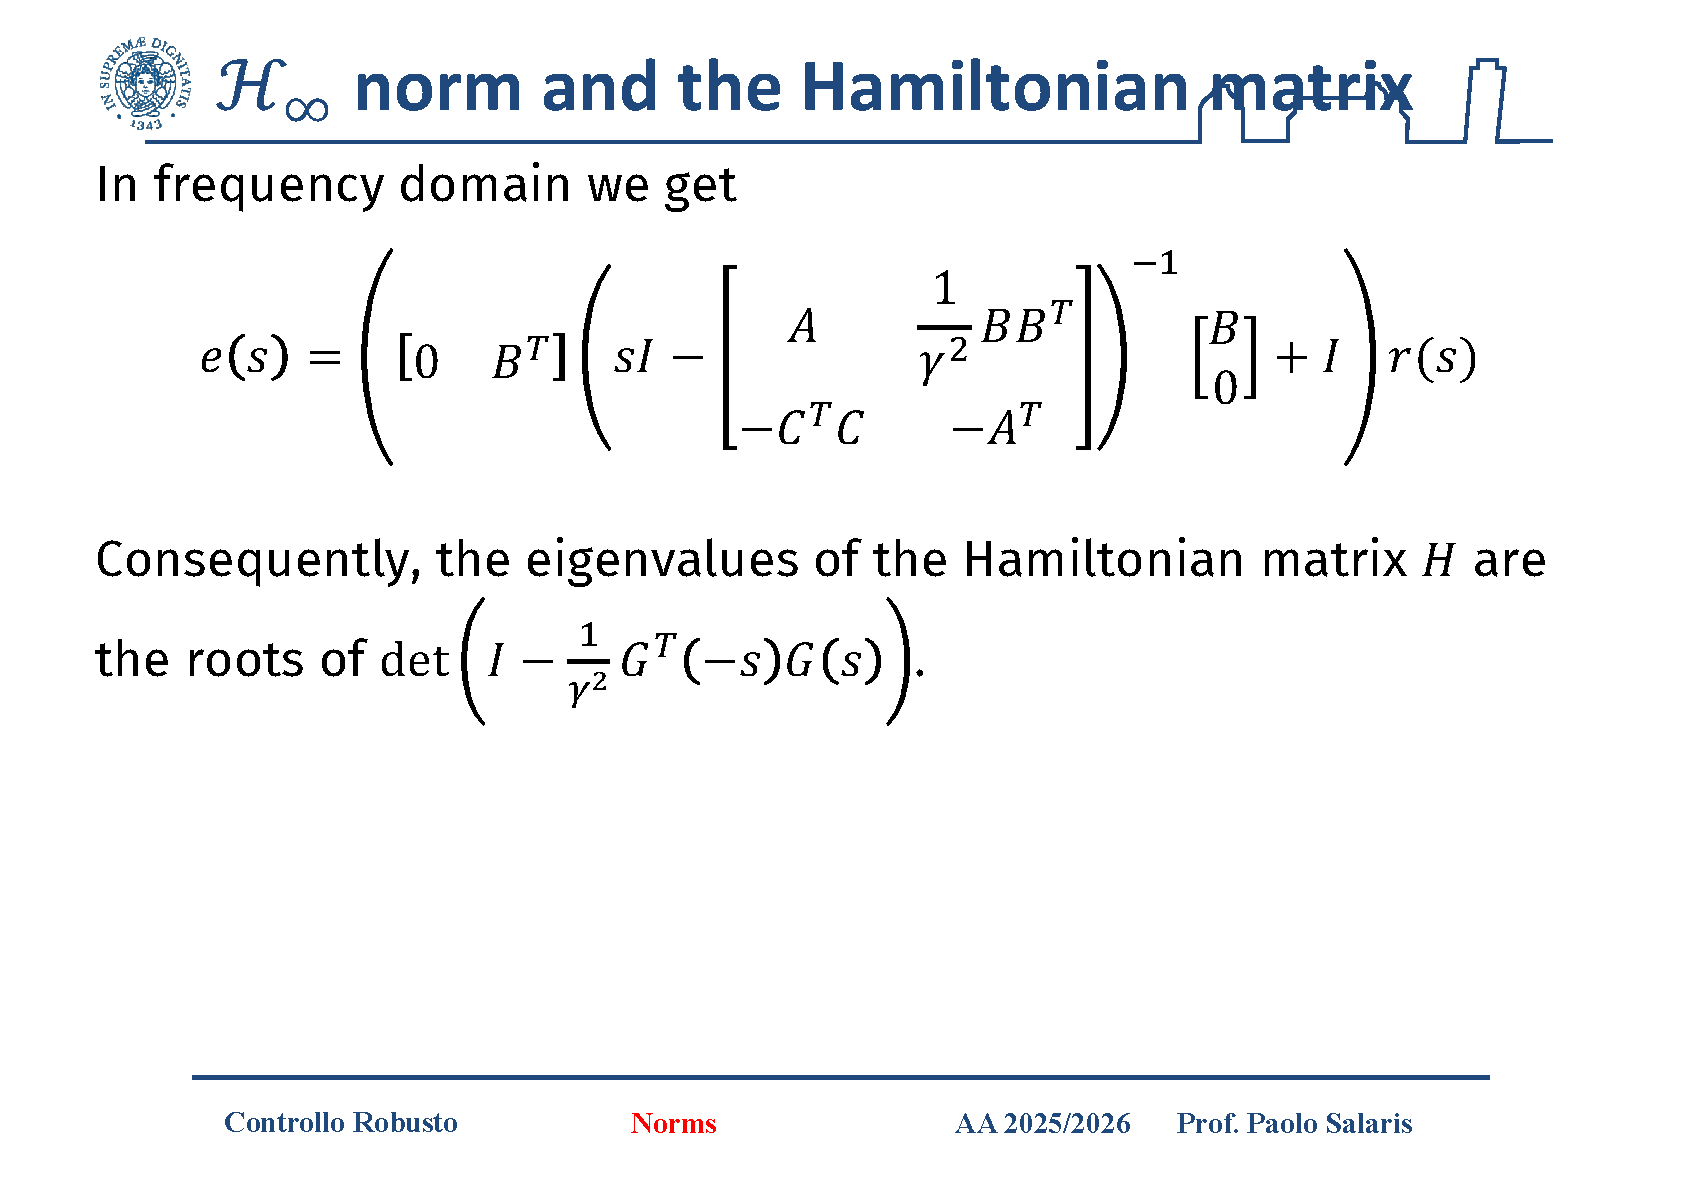
\includegraphics[width=\linewidth]{images8/norms-new-33-53-020.png}
        \caption{Espressione in frequenza di $Q^{-1}(s)$ tramite la risolvente della Hamiltoniana.}
    \end{subfigure}
    \hfill
    \begin{subfigure}{0.48\textwidth}
        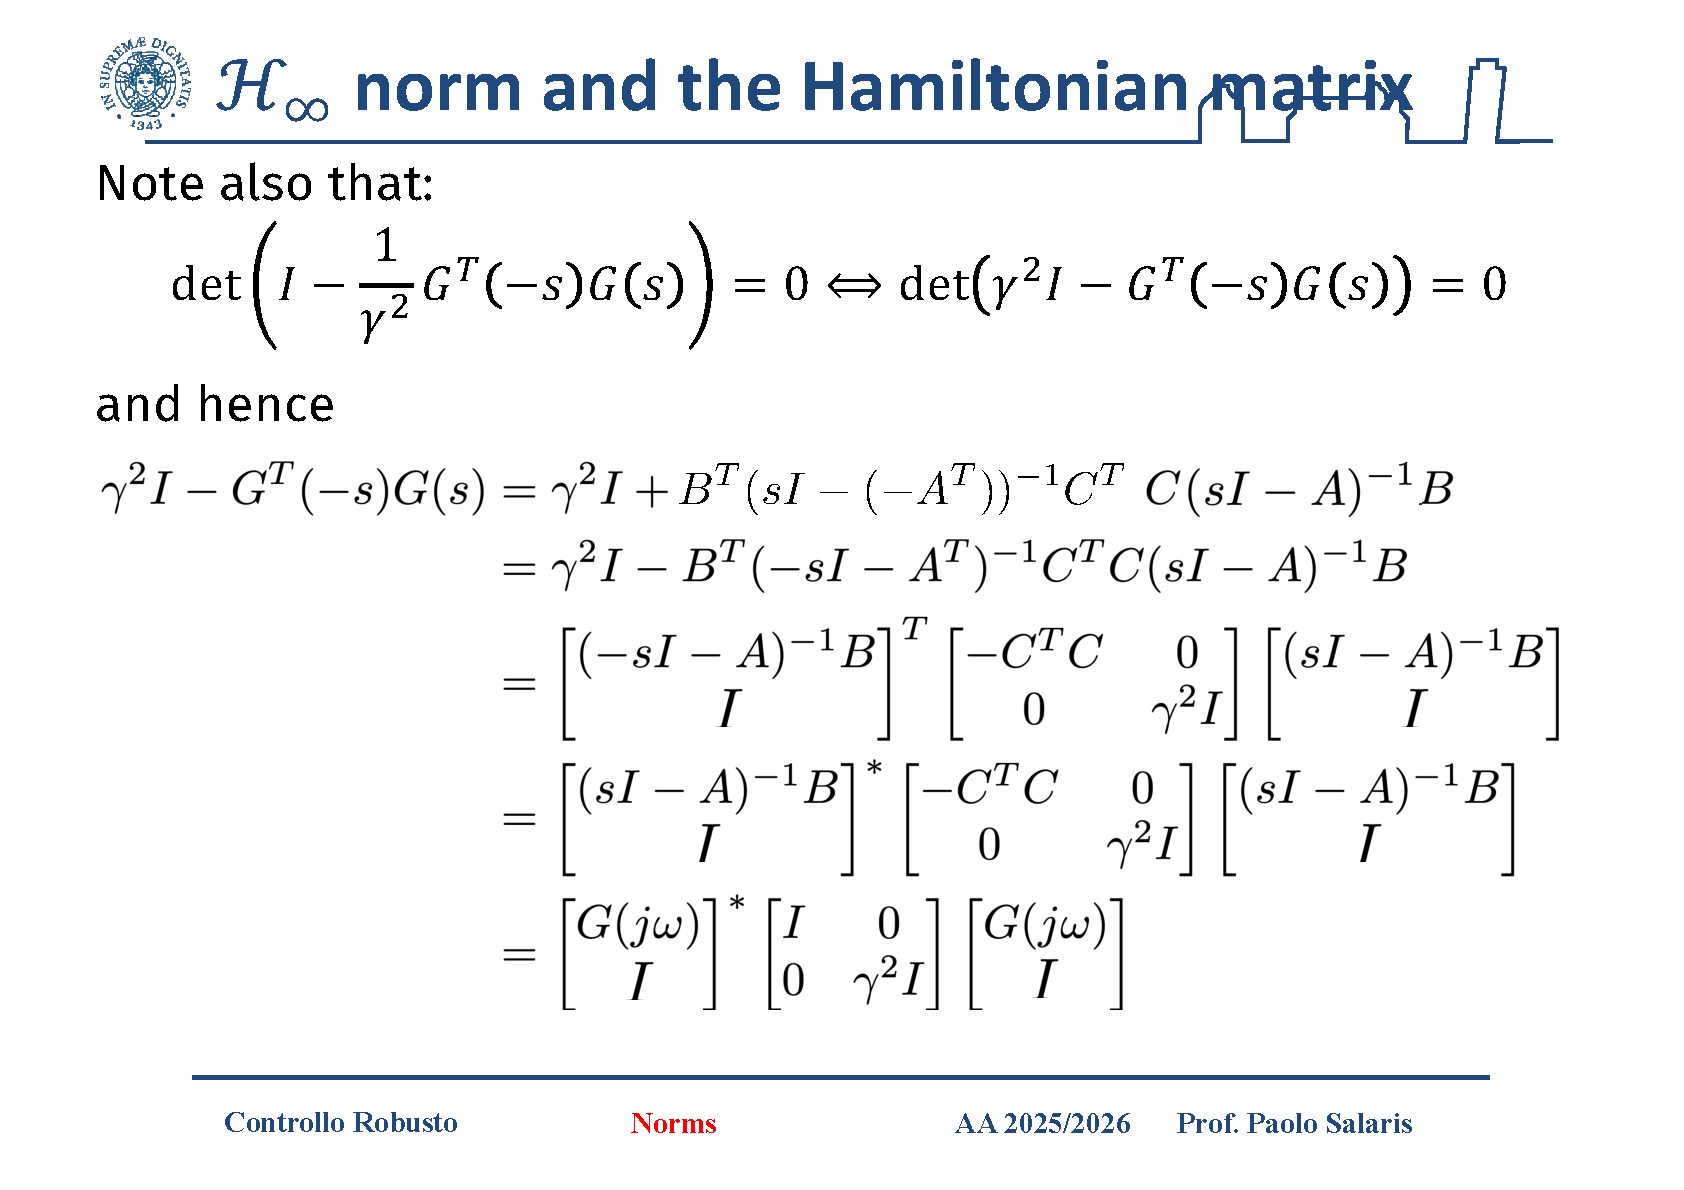
\includegraphics[width=\linewidth]{images8/norms-new-33-53-021.png}
        \caption{Relazione tra zeri del determinante di $Q(s)$ e contatto con la soglia $\gamma$.}
    \end{subfigure}
    \caption{Le ultime slide completano il collegamento tra valori singolari, determinanti e autovalori della Hamiltoniana.}
\end{figure}

\subsection{Sintesi conclusiva della lezione}

La Lezione 8 ha due movimenti principali. Nel primo, le slide mostrano che la norma $H_2$ pu\`o essere calcolata senza integrare direttamente in frequenza: dalla realizzazione di stato si ottengono i gramiani $W_c$ e $W_o$, e questi si calcolano risolvendo equazioni di Lyapunov. Nel secondo, la norma $H_\infty$ viene letta come guadagno energetico peggiore e il suo calcolo viene trasformato in un test a soglia.

Il punto pi\`u importante \`e la sequenza logica finale:
$$
\begin{aligned}
\|G\|_{H_\infty}<\gamma
&\Longleftrightarrow
Q(j\omega)>0\quad\forall\omega,\\
&\Longleftrightarrow
Q(j\omega)\ \text{invertibile}\quad\forall\omega,\\
&\Longleftrightarrow
Q^{-1}(s)\ \text{senza poli su }j\mathbb{R},\\
&\Longleftrightarrow
\mathcal{H}_\gamma\ \text{senza autovalori su }j\mathbb{R}.
\end{aligned}
$$
Questa catena \`e il vero contenuto della seconda met\`a della lezione: sostituisce un controllo su infinite frequenze con un controllo spettrale su una matrice costruita da $A$, $B$, $C$ e dalla soglia $\gamma$.

Sul piano operativo, la lezione lascia quattro risultati:
\begin{itemize}
    \item $\|G\|_{H_2}^2=\operatorname{tr}(CW_cC^T)=\operatorname{tr}(B^TW_oB)$;
    \item $W_c$ e $W_o$ sono soluzioni di due equazioni di Lyapunov;
    \item $\|G\|_{H_\infty}$ \`e il massimo guadagno indotto da $L_2$ a $L_2$;
    \item il test $\|G\|_{H_\infty}<\gamma$ pu\`o essere eseguito tramite la Hamiltoniana $\mathcal{H}_\gamma$.
\end{itemize}
La lezione successiva potr\`a quindi formalizzare questi passaggi con il lemma KYP, il bounded real lemma e le formulazioni LMI/Riccati.

\clearpage
\phantomsection
\section*{Appendice}
\addcontentsline{toc}{section}{Appendice}

\subsection*{Nota sulle convenzioni per la matrice Hamiltoniana}
\phantomsection
\addcontentsline{toc}{subsection}{Nota sulle convenzioni per la matrice Hamiltoniana}

Nel blocco Hamiltoniano delle slide si lavora inizialmente con la realizzazione strettamente propria
$$
G(s)=C(sI-A)^{-1}B,
\qquad D=0.
$$
Per questo la matrice Hamiltoniana compare nella forma semplificata
$$
\mathcal{H}_\gamma
=
\begin{bmatrix}
A & \gamma^{-2}BB^T\\
-C^TC & -A^T
\end{bmatrix}.
$$
Nel caso pi\`u generale, con termine diretto $D\neq 0$, la forma della Hamiltoniana cambia e viene trattata pi\`u comodamente tramite il \emph{bounded real lemma}. Gi\`a in questa lezione, per\`o, compare la condizione preliminare all'infinito:
$$
Q(j\infty)=I-\frac{1}{\gamma^2}D^TD>0,
$$
cio\`e $\bar{\sigma}(D)<\gamma$. Nel testo si \`e quindi mantenuta la Hamiltoniana strettamente propria delle slide, esplicitando separatamente il controllo sul termine diretto.

\subsection*{Riferimento al materiale originale}
\phantomsection
\addcontentsline{toc}{subsection}{Riferimento al materiale originale}

Questa parte del documento \`e una traduzione e rielaborazione estesa delle slide 33--53 del PDF aggiornato ``Norms for signals and systems'', caricato dall'utente come materiale di partenza. La riscrittura segue l'ordine delle slide: gramiani e Lyapunov per $H_2$, spazio di Hardy e norma indotta per $H_\infty$, test a soglia tramite $Q(s)$ e costruzione della matrice Hamiltoniana.

\begin{coverpage}
\centering
{\Huge\bfseries Controllo Robusto\par}
\vspace{0.4em}
{\LARGE Traduzione in italiano e approfondimento\par}
\vspace{0.5em}
{\Large KYP lemma, bounded real lemma e forma Hamiltoniana generale\par}
\vfill
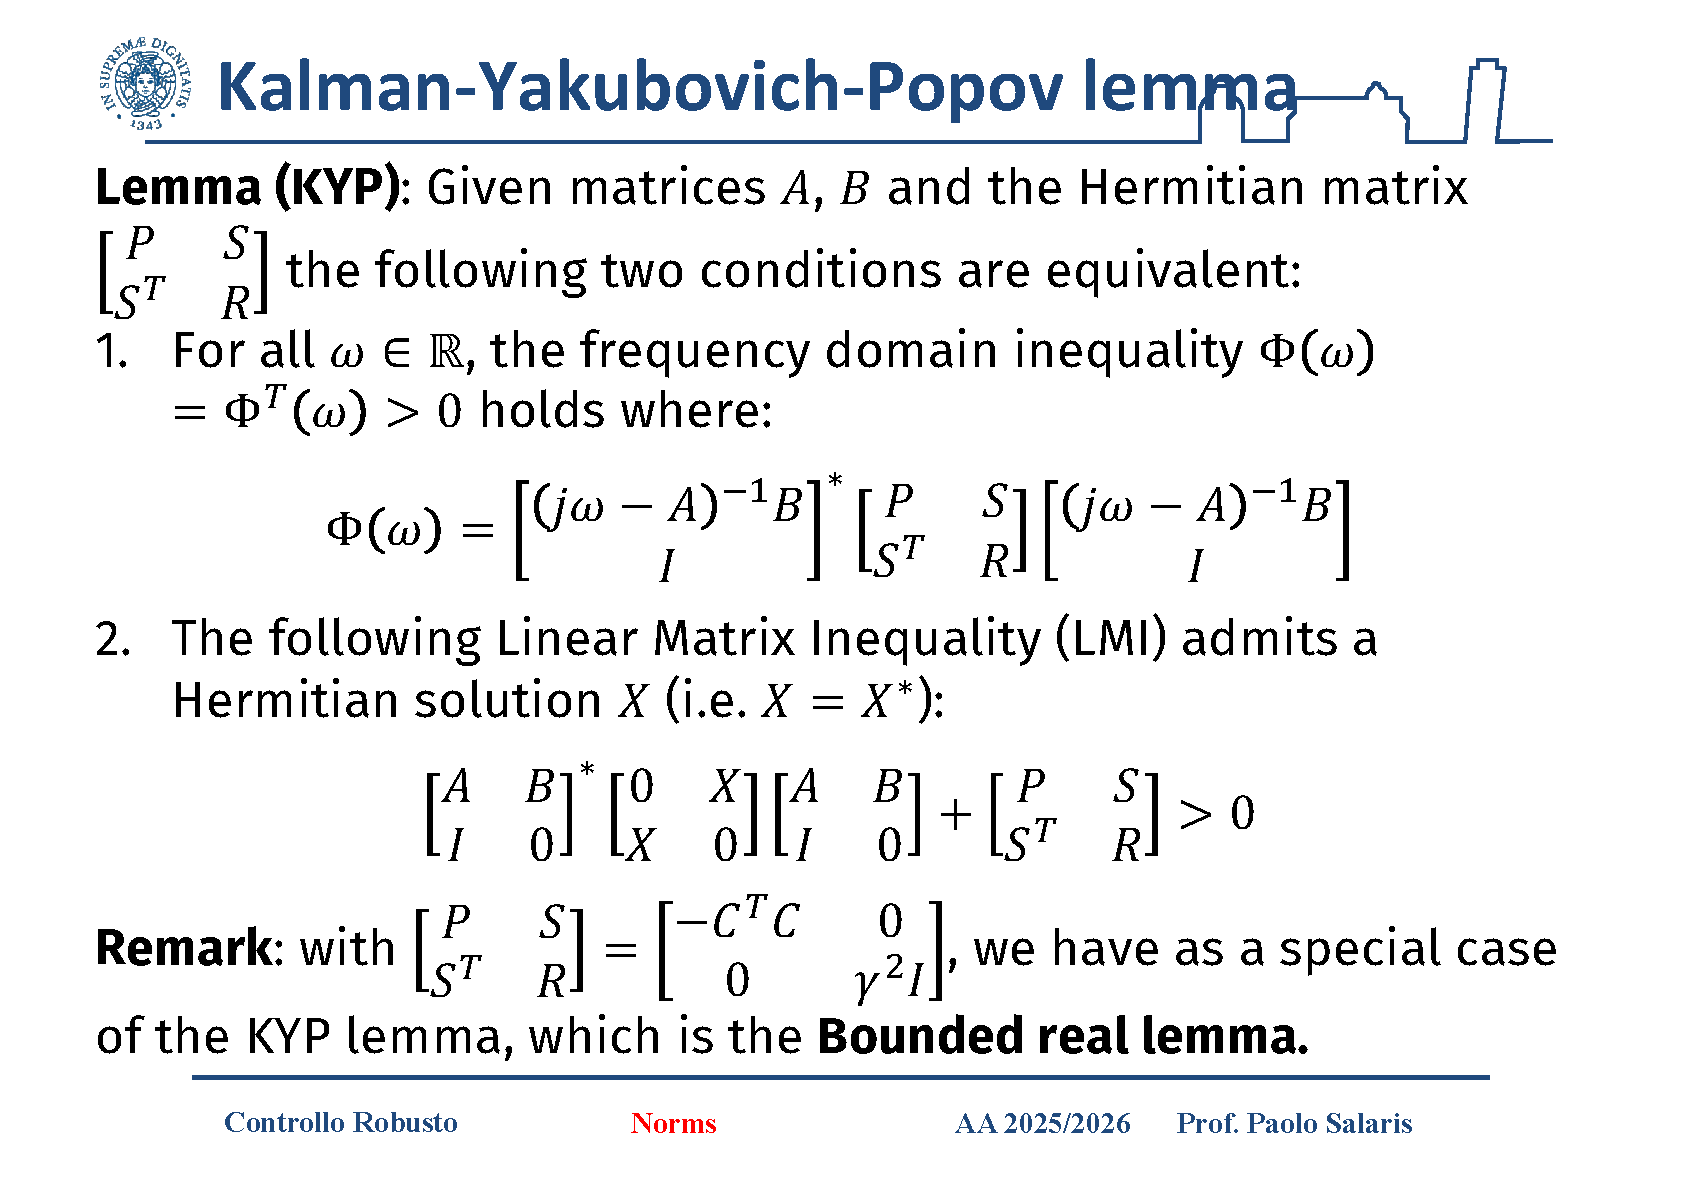
\includegraphics[width=0.78\textwidth]{images9/norms-new-54-59-001.png}
\vfill
\begin{focusbox}
\textbf{Obiettivo del documento.} Questa parte del testo sviluppa la Lezione 9 a partire dalle slide 54--59 del PDF aggiornato ``Norms for signals and systems''. Dopo il test Hamiltoniano introdotto nella Lezione 8, la lezione formalizza il risultato tramite il lemma di Kalman--Yakubovich--Popov, il complemento di Schur, il \emph{bounded real lemma}, la formulazione LMI e la corrispondente equazione di Riccati. L'obiettivo \`e rendere chiaro perch\'e una disuguaglianza in frequenza su infinite $\omega$ possa essere trattata come un problema matriciale finito.
\end{focusbox}
\vfill
{\large Basato sulle slide del corso AA 2025/2026\par}
\end{coverpage}

\section{Lezione 9}

\subsection{Visione d'insieme della lezione}

La Lezione 9 chiude il percorso teorico iniziato con la norma $H_\infty$. Nella Lezione 8 si era visto come il problema
$$
\|G\|_{H_\infty}<\gamma
$$
possa essere trasformato in un test sulla funzione
$$
Q(s)=I-\frac{1}{\gamma^2}G^T(-s)G(s)
$$
e, nel caso strettamente proprio, in un controllo sugli autovalori di una matrice Hamiltoniana. Le slide 54--59 spiegano ora il quadro generale che giustifica questi passaggi: il lemma KYP e il \emph{bounded real lemma}.

\begin{focusbox}
\textbf{Nota di collocazione.} Nel PDF aggiornato, le slide 42--53 sono formalmente associate all'avvio della Lezione 9. In questi appunti sono state per\`o integrate nella Lezione 8, perch\'e completano direttamente la costruzione della matrice Hamiltoniana iniziata l\`i. La Lezione 9 parte quindi dalle slide 54--59 e ne raccoglie la formalizzazione tramite KYP, LMI e Riccati.
\end{focusbox}

Il filo logico della lezione \`e il seguente. Prima si introduce il lemma KYP, che permette di sostituire una disuguaglianza frequenziale valida per ogni $\omega$ con una disuguaglianza matriciale, cio\`e una LMI. Poi si richiama il complemento di Schur, che permette di passare da una LMI a una disuguaglianza di Riccati. Infine si applica tutto questo al caso $H_\infty$, ottenendo il \emph{bounded real lemma} sia nella forma strettamente propria sia nella forma generale con termine diretto $D$.

\begin{keybox}
Il messaggio centrale \`e che il controllo robusto non cerca di verificare infinite condizioni frequenziali una per una. Grazie al lemma KYP, molte condizioni del tipo ``per ogni frequenza'' possono essere trasformate in problemi matriciali finiti, risolvibili numericamente.
\end{keybox}

\subsection{Il lemma di Kalman--Yakubovich--Popov}

Il lemma di Kalman--Yakubovich--Popov, spesso abbreviato in lemma KYP, \`e uno dei risultati strutturali pi\`u importanti della teoria dei sistemi. Nella forma usata dalle slide, si considera una matrice hermitiana
$$
\Pi=
\begin{bmatrix}
P & S\\
S^* & R
\end{bmatrix}
=\Pi^*
$$
e si studia una disuguaglianza nel dominio della frequenza del tipo
$$
\Phi(\omega)
=
\begin{bmatrix}
(j\omega I-A)^{-1}B\\
I
\end{bmatrix}^*
\Pi
\begin{bmatrix}
(j\omega I-A)^{-1}B\\
I
\end{bmatrix}
>0,
\qquad \forall\,\omega\in\mathbb{R}.
$$
Il contenuto del lemma \`e che questa disuguaglianza frequenziale \`e equivalente all'esistenza di una matrice hermitiana $X=X^*$ tale che valga una LMI.

In una forma compatta, la LMI si pu\`o scrivere come
$$
\begin{bmatrix}
A^*X+XA & XB\\
B^*X & 0
\end{bmatrix}
+
\begin{bmatrix}
P & S\\
S^* & R
\end{bmatrix}
>0.
$$
La potenza del lemma \`e tutta qui: una condizione su una funzione di frequenza continua viene ricondotta all'esistenza di una matrice $X$ che soddisfa una disuguaglianza algebrica.

Dal punto di vista del corso, il caso davvero importante \`e quello che porta al \emph{bounded real lemma}. Scegliendo opportunamente la matrice $\Pi$ in modo da rappresentare la disuguaglianza
$$
\gamma^2I-G^T(-j\omega)G(j\omega)>0,
$$
il lemma KYP diventa esattamente lo strumento che collega $\|G\|_{H_\infty}<\gamma$ a una LMI.

\begin{figure}[H]
    \centering
    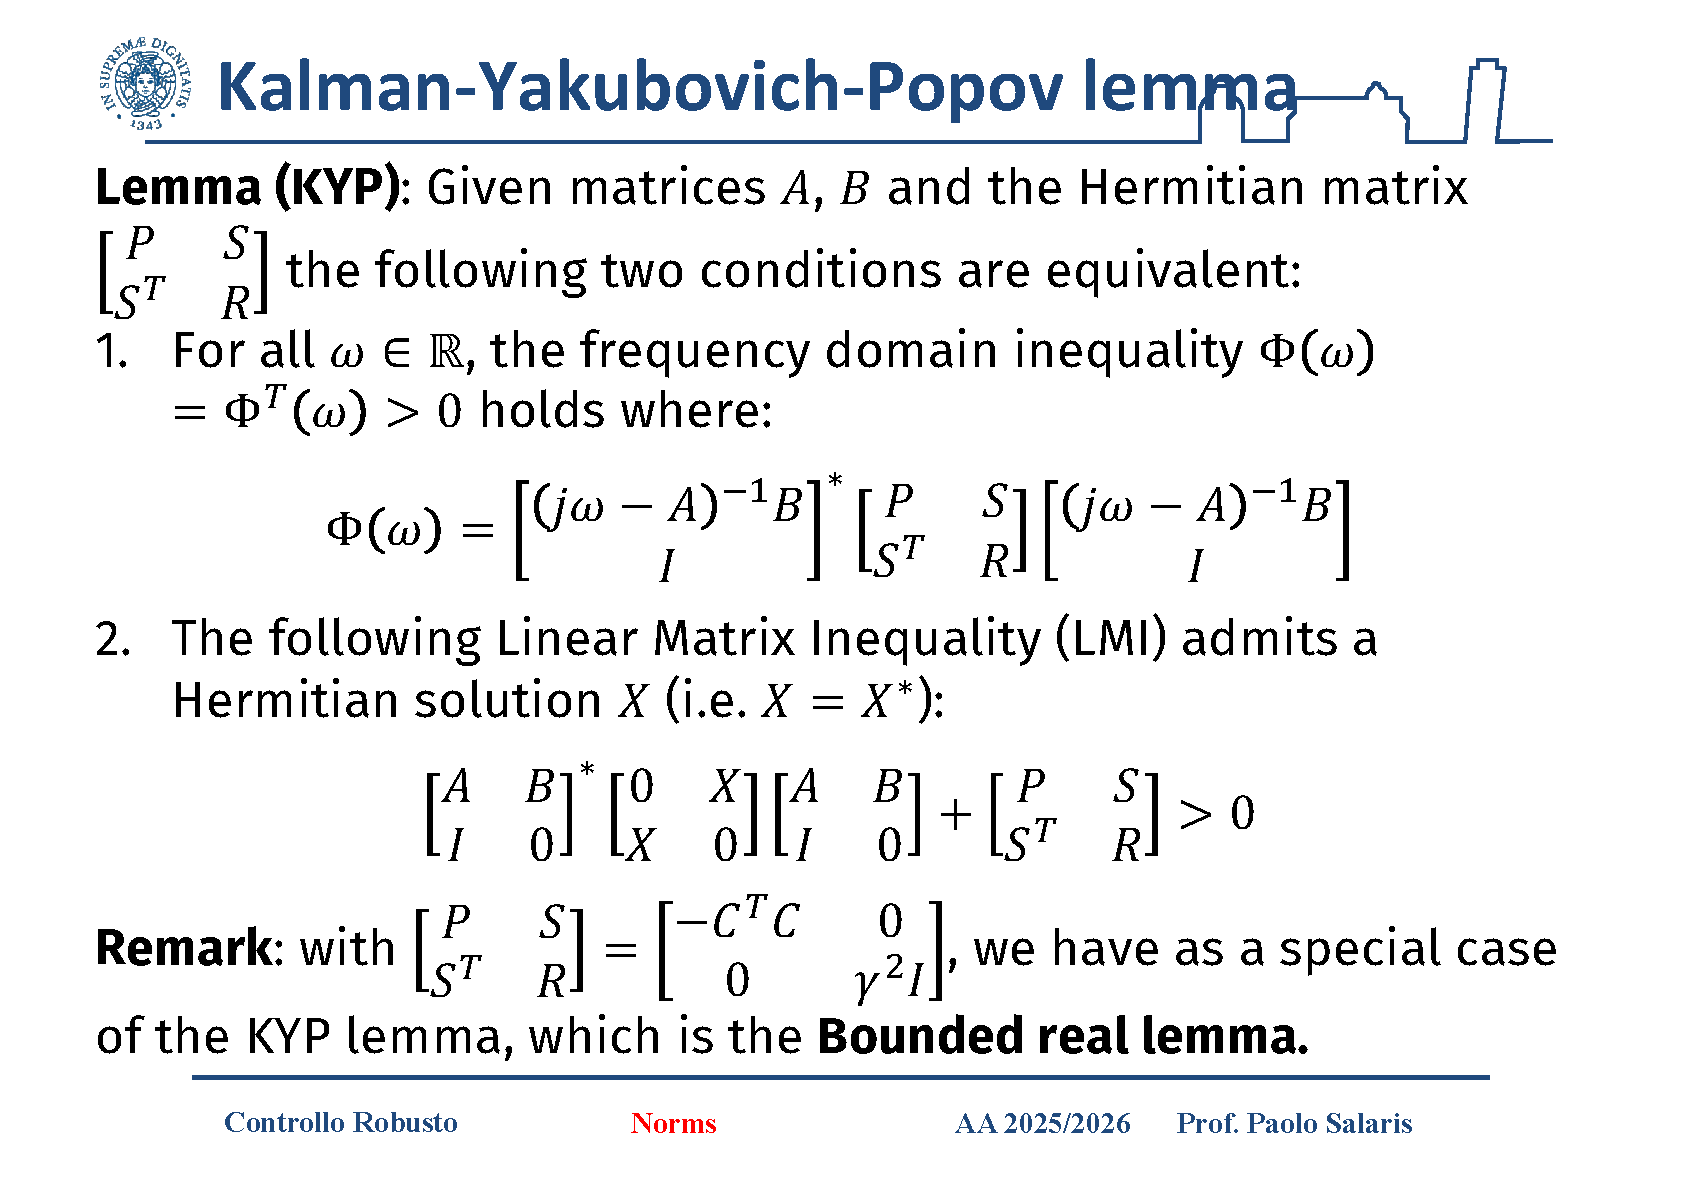
\includegraphics[width=0.82\textwidth]{images9/norms-new-54-59-001.png}
    \caption{Il lemma KYP trasforma una disuguaglianza frequenziale valida per ogni $\omega$ in una LMI con incognita hermitiana $X$.}
\end{figure}

\begin{focusbox}
\textbf{Interpretazione.} La frequenza $\omega$ non sparisce magicamente: viene ``assorbita'' nella struttura dinamica $(j\omega I-A)^{-1}B$. Il lemma KYP dice che, sotto ipotesi appropriate, controllare quella struttura per ogni frequenza equivale a trovare una matrice di certificato $X$.
\end{focusbox}

\subsection{Complemento di Schur e passaggio a Riccati}

La slide successiva richiama il complemento di Schur, che \`e lo strumento algebrico usato continuamente per passare da LMI a disuguaglianze di Riccati. Data una matrice a blocchi
$$
M=
\begin{bmatrix}
A & B\\
C & D
\end{bmatrix},
$$
con $D$ invertibile, il complemento di Schur di $D$ in $M$ \`e
$$
M/D=A-BD^{-1}C.
$$
Analogamente, se $A$ \`e invertibile, il complemento di Schur di $A$ \`e
$$
M/A=D-CA^{-1}B.
$$

Applicando questa identit\`a alla LMI del lemma KYP, si ottiene una disuguaglianza del tipo
$$
XA+A^*X+P-(XB+S)R^{-1}(B^*X+S^*)>0,
$$
quando il blocco $R$ \`e invertibile e si usa la convenzione di segno delle slide. Se si sostituisce la disuguaglianza con l'uguaglianza, si ottiene una equazione algebrica di Riccati generalizzata:
$$
XA+A^*X+P-(XB+S)R^{-1}(B^*X+S^*)=0.
$$

Questo passaggio \`e fondamentale perch\'e mostra il legame tra tre linguaggi che nel controllo robusto compaiono continuamente:
\begin{itemize}
    \item disuguaglianze in frequenza;
    \item disuguaglianze matriciali lineari;
    \item equazioni di Riccati.
\end{itemize}
Non sono tre teorie separate, ma tre rappresentazioni dello stesso contenuto di dissipativit\`a o di guadagno limitato.

\begin{figure}[H]
    \centering
    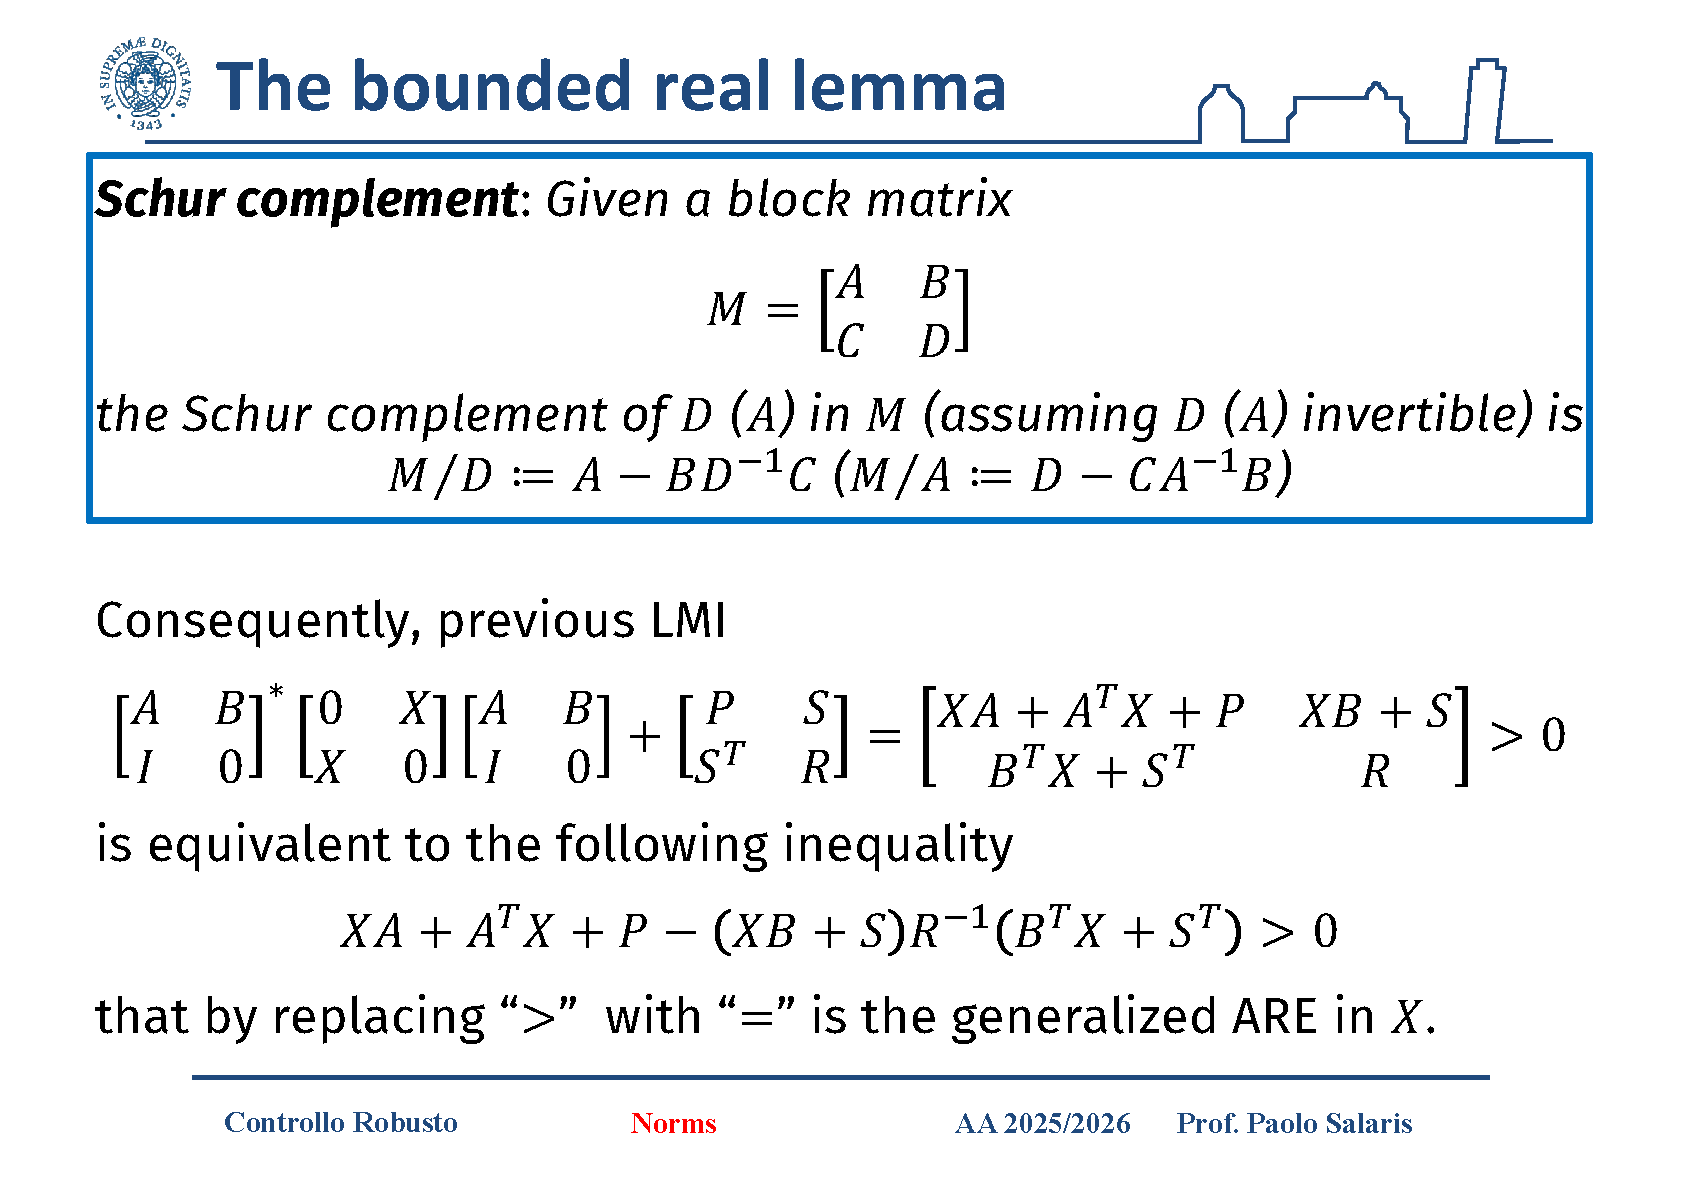
\includegraphics[width=0.82\textwidth]{images9/norms-new-54-59-002.png}
    \caption{Il complemento di Schur permette di trasformare una LMI in una disuguaglianza di Riccati, e l'uguaglianza associata in una ARE generalizzata.}
\end{figure}

\subsection{Bounded real lemma nel caso strettamente proprio}

Le slide riassumono poi il caso strettamente proprio gi\`a preparato nella Lezione 8. Supponiamo
$$
G(s)=C(sI-A)^{-1}B,
\qquad D=0,
$$
con $A$ asintoticamente stabile. Allora la condizione
$$
\|G\|_{H_\infty}<\gamma
$$
\`e equivalente all'esistenza di una matrice simmetrica positiva $P=P^T>0$ tale che
$$
\begin{bmatrix}
A^TP+PA+C^TC & PB\\
B^TP & -\gamma^2I
\end{bmatrix}
<0.
$$
Questa \`e la forma LMI del \emph{bounded real lemma} per sistemi strettamente propri.

Applicando il complemento di Schur al blocco $-\gamma^2I$, la LMI \`e equivalente alla disuguaglianza di Riccati
$$
A^TP+PA+C^TC+\frac{1}{\gamma^2}PBB^TP<0.
$$
Se si sostituisce il simbolo $<$ con $=$, si ottiene l'equazione di Riccati associata:
$$
A^TP+PA+C^TC+\frac{1}{\gamma^2}PBB^TP=0.
$$

Il collegamento con la Hamiltoniana della Lezione 8 \`e diretto. Nel caso $D=0$, la matrice
$$
\mathcal{H}_\gamma=
\begin{bmatrix}
A & \gamma^{-2}BB^T\\
-C^TC & -A^T
\end{bmatrix}
$$
non deve avere autovalori sull'asse immaginario. Questo criterio e la LMI sono due facce dello stesso risultato: il primo guarda agli autovalori di una matrice strutturata, la seconda cerca un certificato matriciale $P$.

\begin{figure}[H]
    \centering
    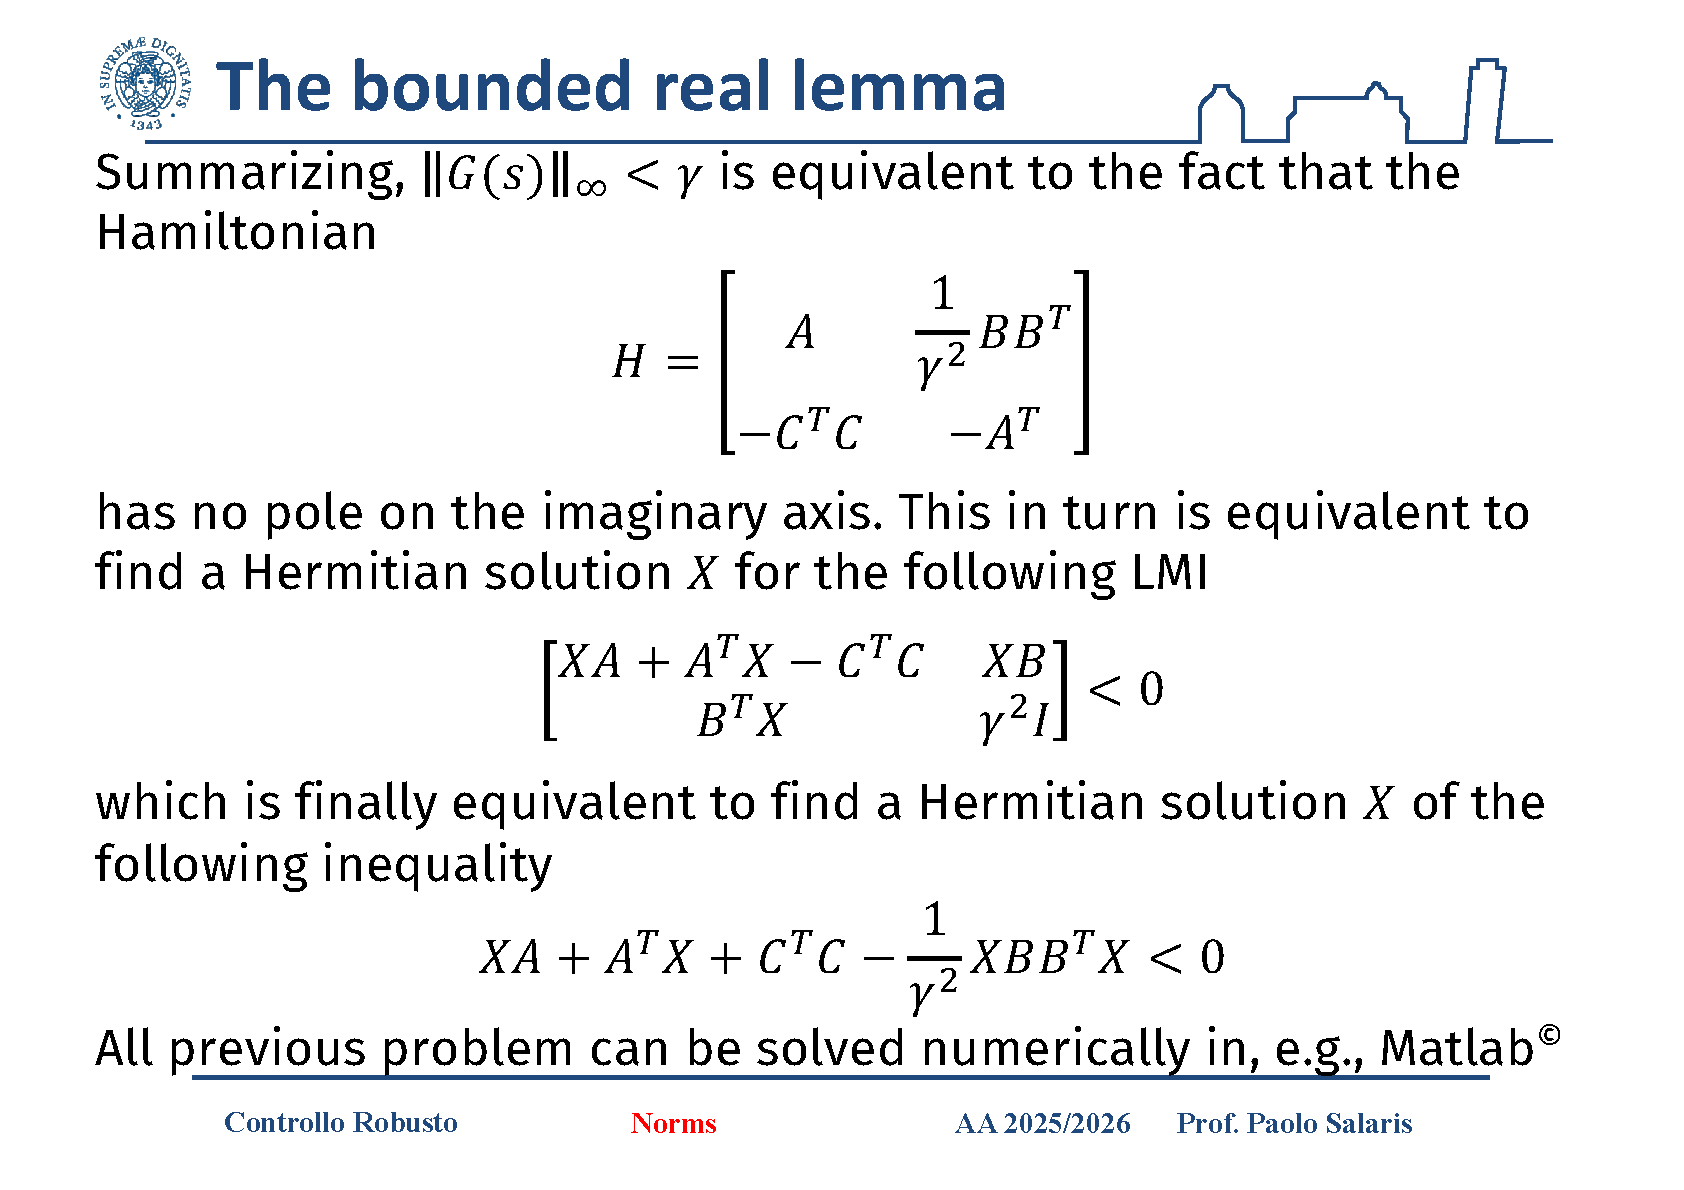
\includegraphics[width=0.82\textwidth]{images9/norms-new-54-59-003.png}
    \caption{Nel caso strettamente proprio, $\|G\|_{H_\infty}<\gamma$ pu\`o essere certificato con una LMI, una Riccati oppure una Hamiltoniana senza autovalori immaginari.}
\end{figure}

\subsection{Formulazione LMI per sistemi propri}

La slide successiva passa al caso pi\`u generale
$$
G(s)=C(sI-A)^{-1}B+D,
$$
sempre con $A$ asintoticamente stabile. Qui il termine diretto $D$ non pu\`o essere ignorato, perch\'e rappresenta il comportamento del sistema ad alta frequenza:
$$
G(j\infty)=D.
$$
Per questo, prima ancora di controllare la dinamica, \`e necessario che il guadagno diretto sia inferiore alla soglia $\gamma$.

La ricerca della norma $H_\infty$ pu\`o essere formulata come il seguente problema di ottimizzazione LMI:
$$
\min \gamma
$$
soggetto all'esistenza di una matrice
$$
P=P^T>0
$$
tale che
$$
\begin{bmatrix}
A^TP+PA & PB & C^T\\
B^TP & -\gamma^2I & D^T\\
C & D & -I
\end{bmatrix}
<0.
$$
Questa \`e una forma molto usata numericamente: si cerca il pi\`u piccolo $\gamma$ che rende fattibile la LMI.

Il significato pratico \`e importante. Invece di campionare $\bar{\sigma}(G(j\omega))$ e sperare di non perdere il picco, si risolve un problema convesso in cui $\gamma$ rappresenta direttamente il limite superiore sul guadagno $H_\infty$. Questo \`e uno dei motivi per cui le LMI sono diventate uno strumento centrale nel controllo robusto moderno.

\begin{figure}[H]
    \centering
    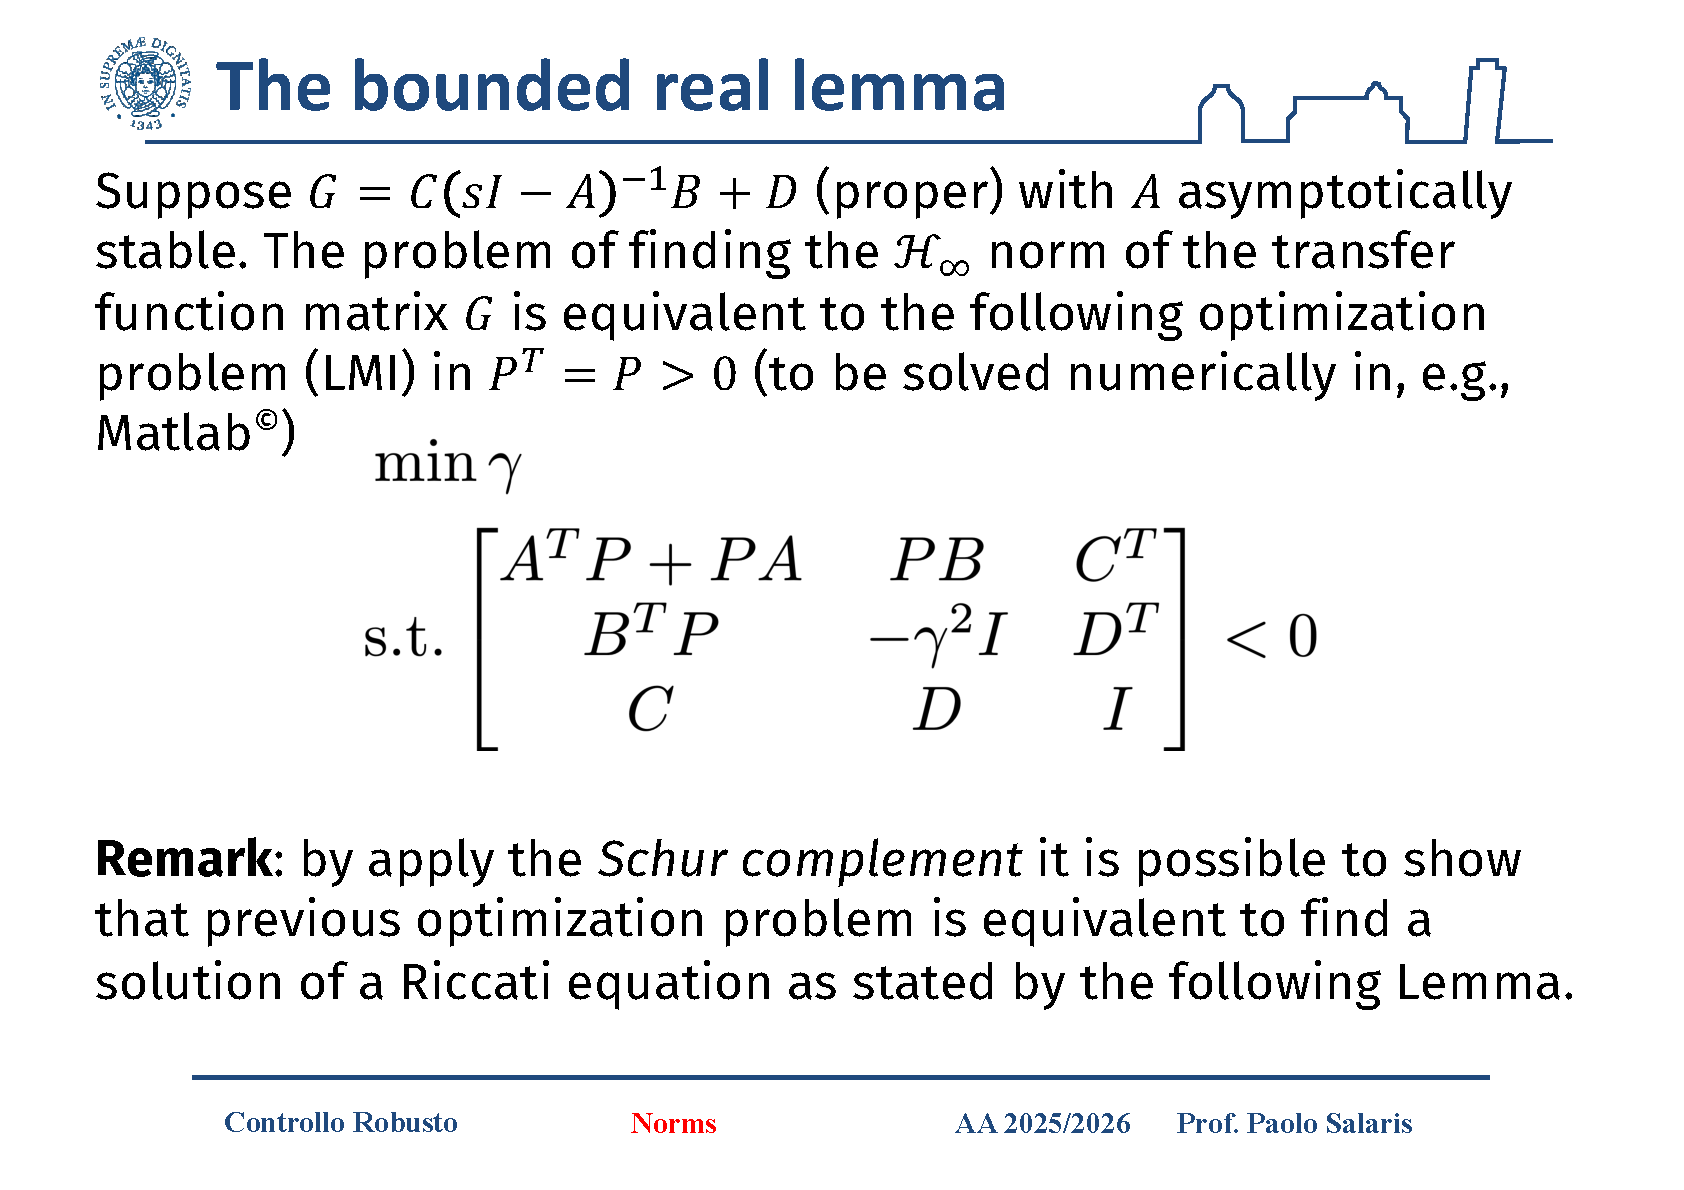
\includegraphics[width=0.82\textwidth]{images9/norms-new-54-59-004.png}
    \caption{Per sistemi propri, il calcolo di $\|G\|_{H_\infty}$ pu\`o essere impostato come problema LMI di minimizzazione della soglia $\gamma$.}
\end{figure}

\subsection{Forma di Riccati del bounded real lemma}

Applicando il complemento di Schur alla LMI del caso proprio si ottiene la formulazione di Riccati riportata nelle slide. Si definisce
$$
R=\gamma^2I-D^TD.
$$
La prima condizione \`e
$$
R>0,
$$
equivalente a
$$
\|D\|<\gamma
\qquad\text{oppure}\qquad
\bar{\sigma}(D)<\gamma.
$$
Questa \`e la condizione all'infinito gi\`a anticipata nella Lezione 8.

La seconda condizione \`e l'esistenza di una soluzione hermitiana $P=P^T$ dell'equazione di Riccati
$$
P(A+BR^{-1}D^TC)
+
(A+BR^{-1}D^TC)^TP
+
PBR^{-1}B^TP
+
C^T(I+DR^{-1}D^T)C
=0,
$$
tale che la matrice chiusa
$$
A+BR^{-1}(D^TC+B^TP)
$$
sia asintoticamente stabile. Quando tale soluzione esiste, le slide osservano che si ottiene $P=P^T>0$.

Questa versione \`e meno immediata della LMI, ma \`e molto utile per capire la struttura del problema. La Riccati mostra infatti come il termine diretto $D$ modifichi sia la dinamica efficace, tramite $BR^{-1}D^TC$, sia il termine quadratico in $P$, tramite $BR^{-1}B^T$.

\begin{figure}[H]
    \centering
    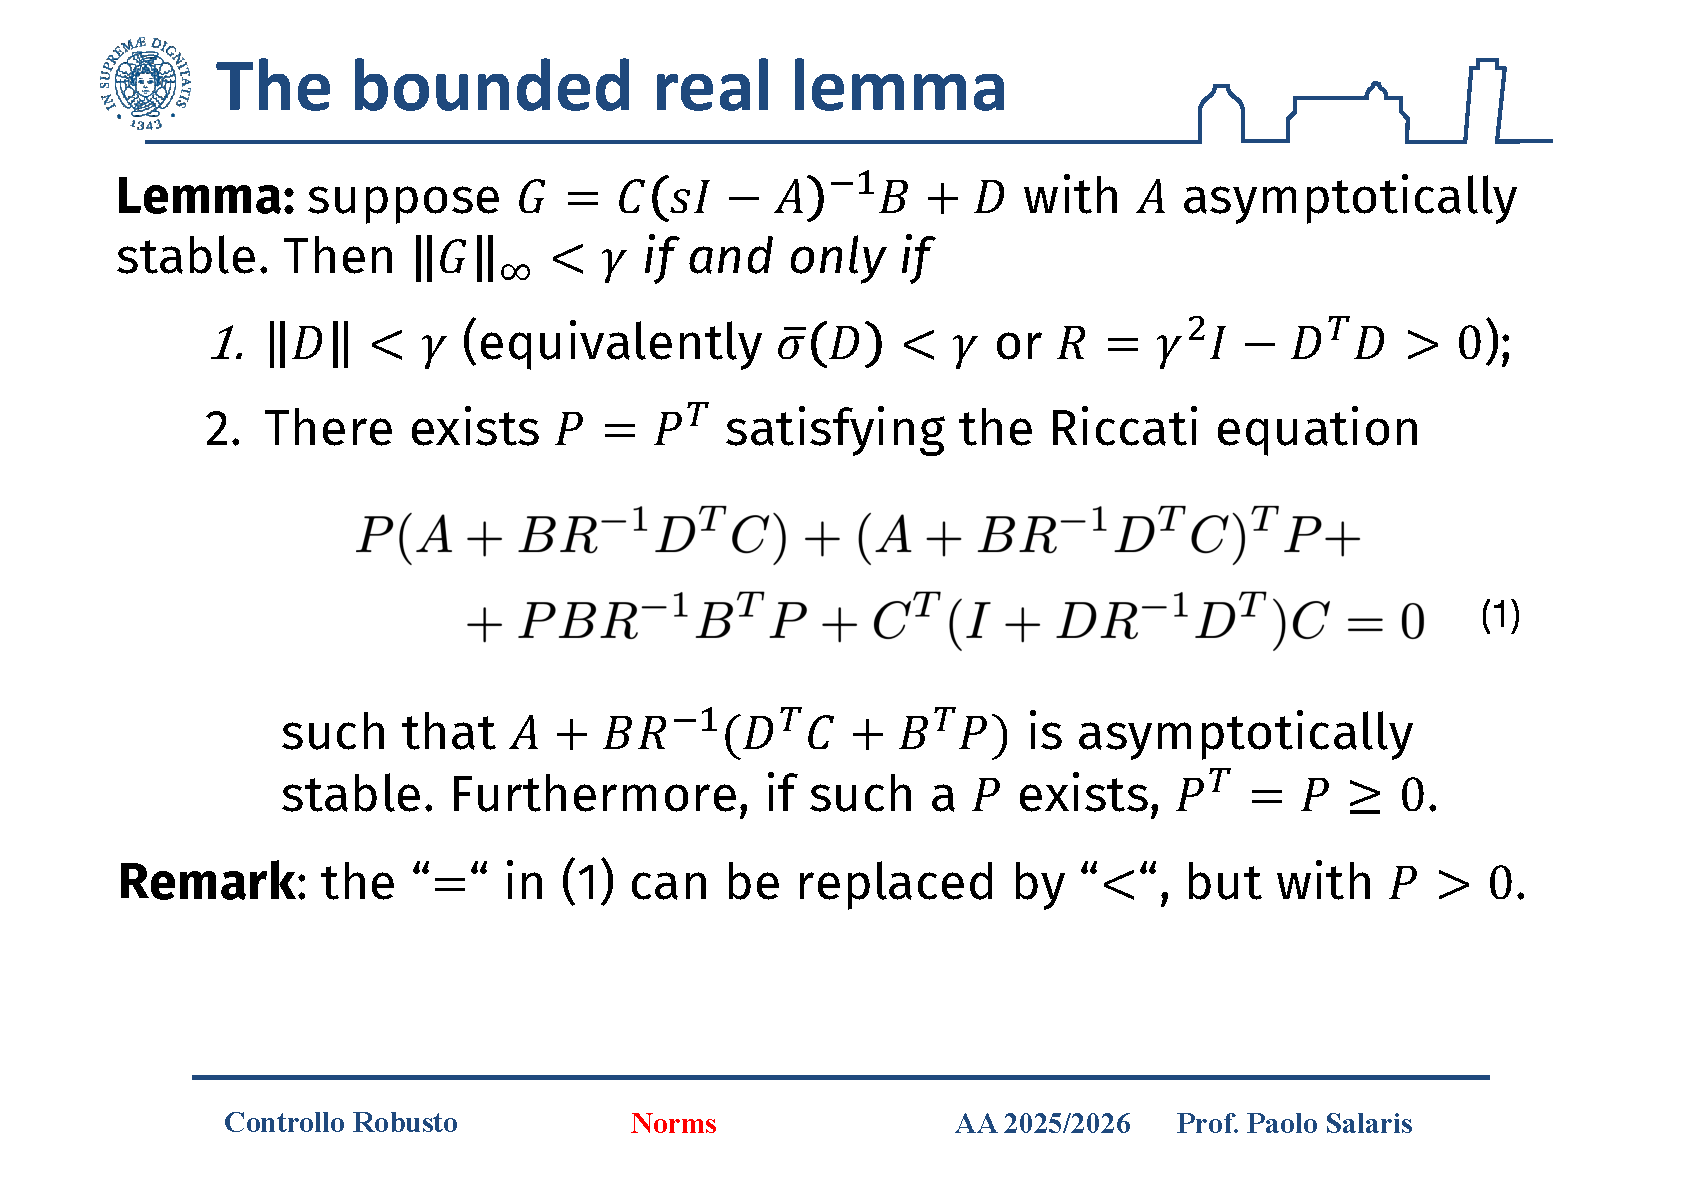
\includegraphics[width=0.82\textwidth]{images9/norms-new-54-59-005.png}
    \caption{La forma di Riccati del bounded real lemma introduce la matrice $R=\gamma^2I-D^TD$ e una condizione di stabilit\`a sulla dinamica chiusa associata.}
\end{figure}

\subsection{Forma Hamiltoniana generale}

L'ultima slide esprime lo stesso risultato in forma Hamiltoniana. Supponiamo ancora
$$
G(s)=C(sI-A)^{-1}B+D,
$$
con $A$ asintoticamente stabile. Allora
$$
\|G\|_{H_\infty}<\gamma
$$
se e solo se valgono due condizioni:
\begin{itemize}
    \item $\|D\|<\gamma$, cio\`e $R=\gamma^2I-D^TD>0$;
    \item la matrice Hamiltoniana
\end{itemize}
$$
\mathcal{H}_\gamma=
\begin{bmatrix}
A+BR^{-1}D^TC & BR^{-1}B^T\\
-C^T(I+DR^{-1}D^T)C & -(A+BR^{-1}D^TC)^T
\end{bmatrix}
$$
non ha autovalori sull'asse immaginario.

Questa formula generalizza perfettamente quella della Lezione 8. Se $D=0$, allora
$$
R=\gamma^2I,
$$
e si recupera
$$
\mathcal{H}_\gamma=
\begin{bmatrix}
A & \gamma^{-2}BB^T\\
-C^TC & -A^T
\end{bmatrix}.
$$
Il caso con $D\neq0$ aggiunge quindi solo le correzioni necessarie per tenere conto del guadagno diretto.

La slide finale osserva anche che non c'\`e perdita di generalit\`a nel porre spesso $\gamma=1$. Infatti
$$
\|G\|_{H_\infty}<\gamma
\qquad\Longleftrightarrow\qquad
\|\gamma^{-1}G\|_{H_\infty}<1.
$$
Questo significa che molte dimostrazioni possono essere semplificate normalizzando il problema rispetto alla soglia unitaria.

\begin{figure}[H]
    \centering
    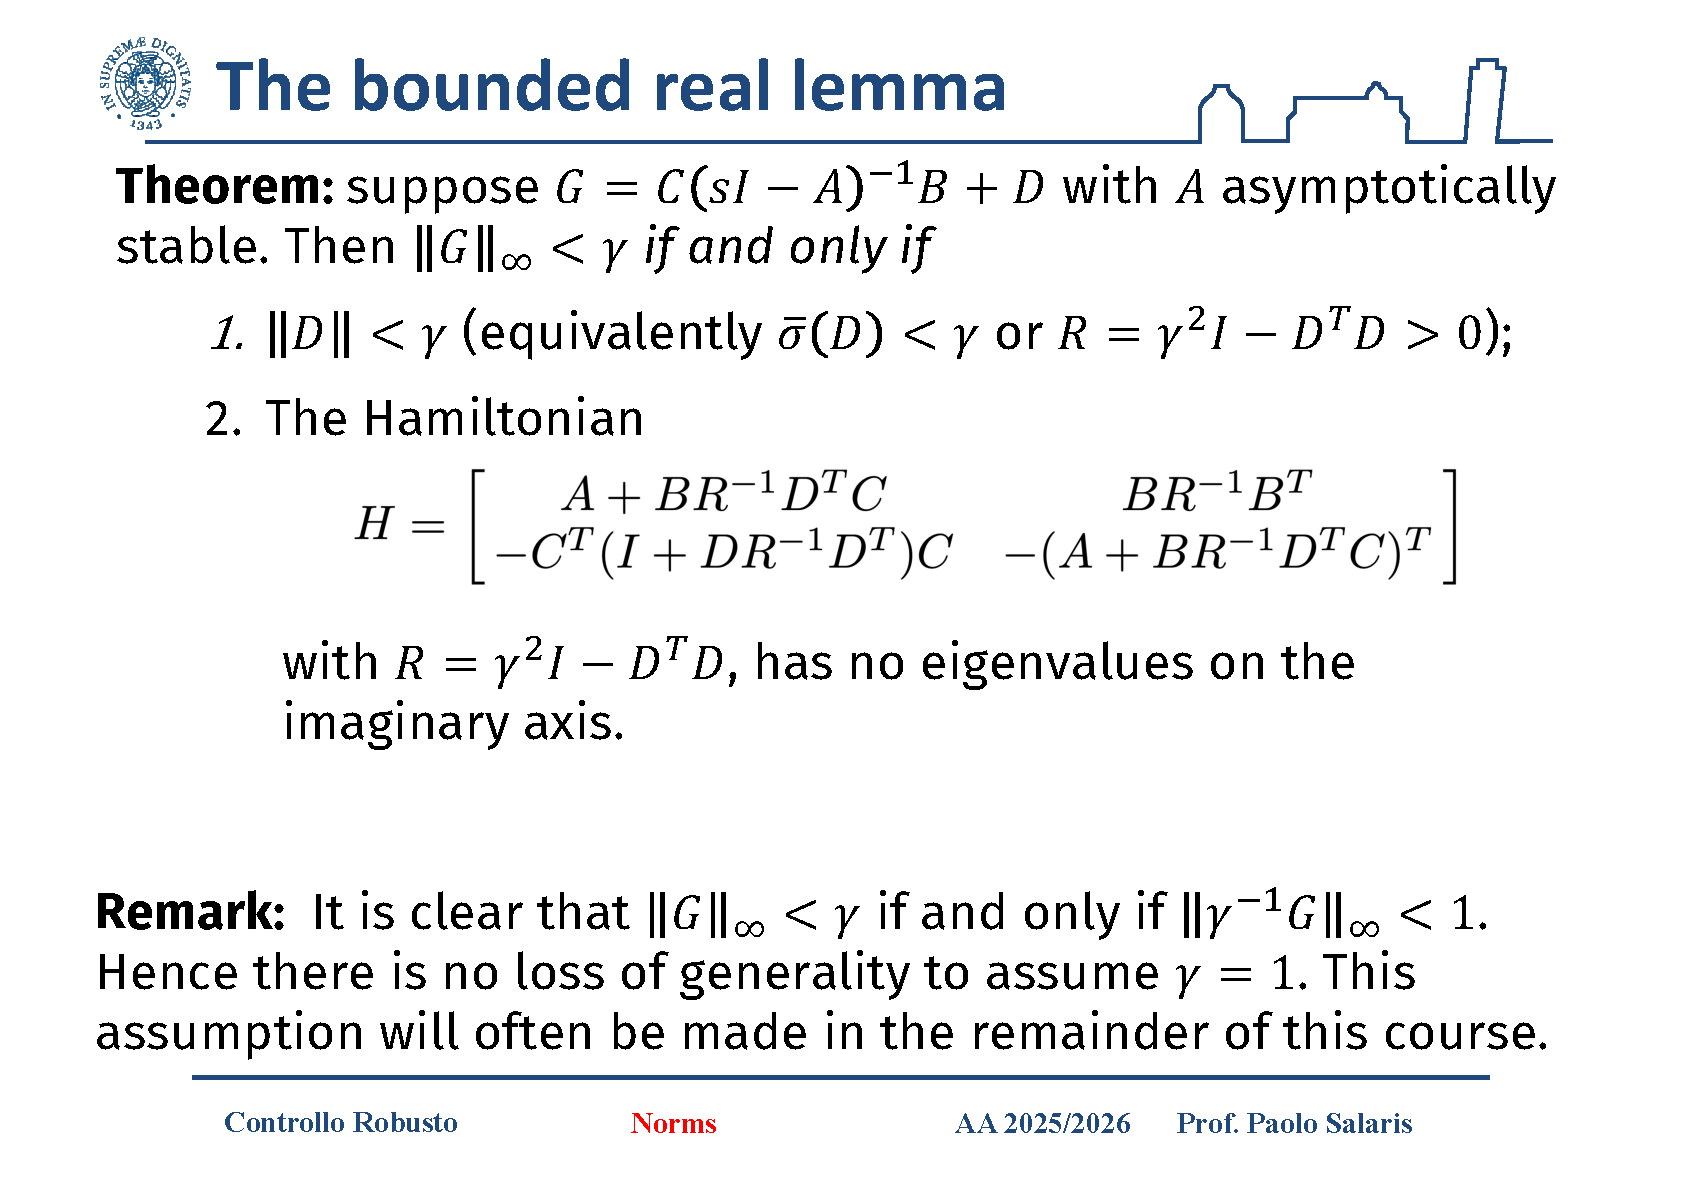
\includegraphics[width=0.82\textwidth]{images9/norms-new-54-59-006.png}
    \caption{La forma Hamiltoniana generale del bounded real lemma include il termine diretto $D$ tramite $R=\gamma^2I-D^TD$.}
\end{figure}

\subsection{Sintesi conclusiva della lezione}

La Lezione 9 formalizza il risultato che era stato costruito in modo operativo nella Lezione 8. Il test su $\|G\|_{H_\infty}<\gamma$ non \`e soltanto un trucco numerico basato sulla Hamiltoniana: \`e una conseguenza del lemma KYP e del bounded real lemma. Questi risultati spiegano perch\'e una specifica frequenziale globale possa essere certificata con una matrice $P$, una LMI, una Riccati o una Hamiltoniana.

Dal punto di vista concettuale, il passaggio decisivo \`e questo: il controllo robusto trasforma requisiti su tutti i segnali e tutte le frequenze in certificati matriciali finiti. Questo \`e ci\`o che rende possibile progettare e verificare sistemi complessi senza dover controllare manualmente ogni frequenza.

Sul piano operativo, la lezione lascia tre strumenti fondamentali:
\begin{itemize}
    \item il lemma KYP come ponte tra frequenza e LMI;
    \item il complemento di Schur come ponte tra LMI e Riccati;
    \item il bounded real lemma come certificato equivalente per $\|G\|_{H_\infty}<\gamma$.
\end{itemize}

\clearpage
\phantomsection
\section*{Appendice}
\addcontentsline{toc}{section}{Appendice}

\subsection*{Nota sulle convenzioni di segno nelle LMI}
\phantomsection
\addcontentsline{toc}{subsection}{Nota sulle convenzioni di segno nelle LMI}

Nel testo si \`e usata la convenzione standard del \emph{bounded real lemma} in cui la LMI viene scritta come matrice negativa definita. Le slide, in alcuni passaggi del lemma KYP, usano invece una forma equivalente con matrice positiva definita. Le due scritture sono compatibili: basta moltiplicare la disuguaglianza per $-1$ e ridefinire coerentemente i blocchi $P,S,R$ della matrice hermitiana $\Pi$.

\subsection*{Riferimento al materiale originale}
\phantomsection
\addcontentsline{toc}{subsection}{Riferimento al materiale originale}

Questa parte del documento \`e una traduzione e rielaborazione estesa delle slide 54--59 del PDF aggiornato ``Norms for signals and systems'', caricato dall'utente come materiale di partenza.

\begin{coverpage}
\centering
{\Huge\bfseries Controllo Robusto\par}
\vspace{0.4em}
{\LARGE Traduzione in italiano e approfondimento\par}
\vspace{0.5em}
{\Large Calcolo della norma $H_\infty$, confronto con $H_2$ e norma di Hankel\par}
\vfill
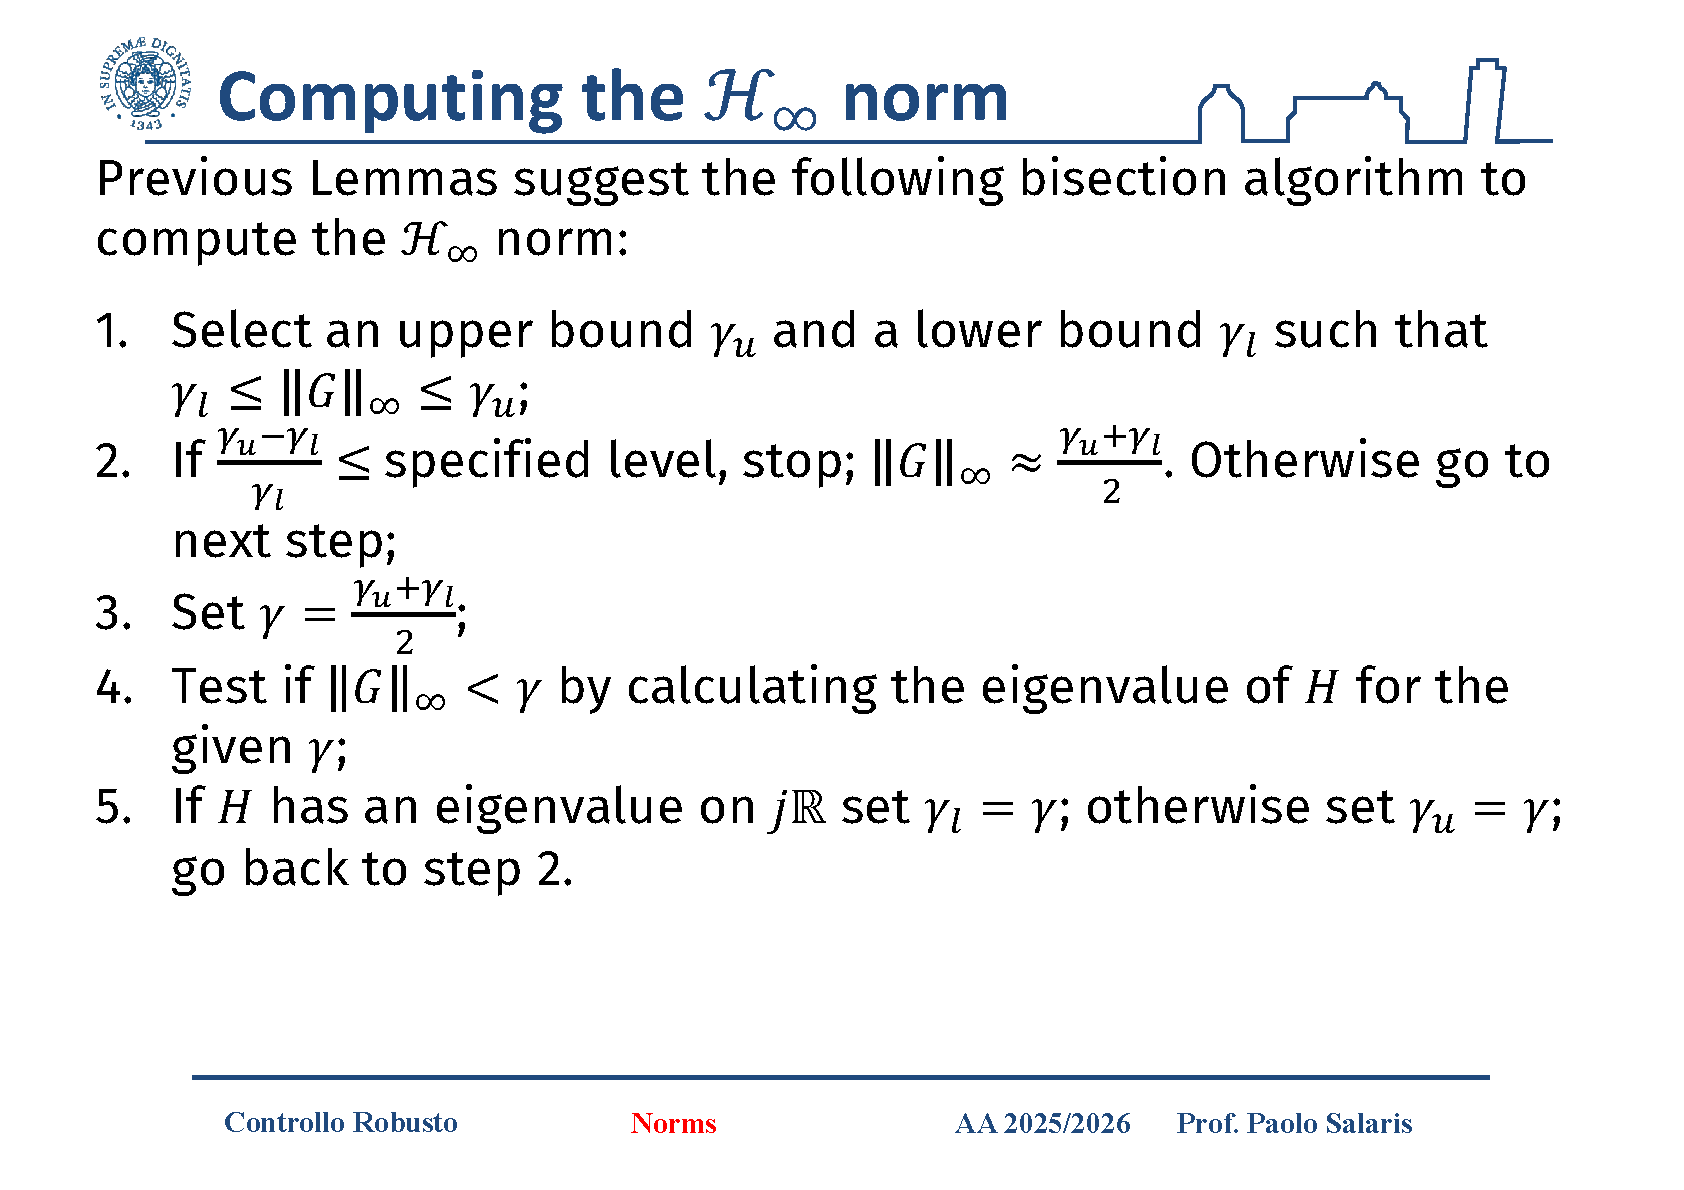
\includegraphics[width=0.78\textwidth]{images10/norms-new-60-76-001.png}
\vfill
\begin{focusbox}
\textbf{Obiettivo del documento.} Questa parte degli appunti segue le slide 60--76 del PDF aggiornato. Dopo il bounded real lemma, la domanda diventa operativa: come si individua numericamente o analiticamente la soglia $\|G\|_{H_\infty}$? La lezione costruisce l'algoritmo di bisezione sulla Hamiltoniana, mostra come Routh--Hurwitz recupera la stessa soglia in esempi piccoli, chiarisce cosa distingue $H_\infty$ da $H_2$ e introduce la norma di Hankel come misura dell'energia immagazzinata nello stato.
\end{focusbox}
\vfill
{\large Basato sulle slide del corso AA 2025/2026\par}
\end{coverpage}

\section{Lezione 10}

\subsection{Visione d'insieme della lezione}

La Lezione 9 ha chiuso il cerchio teorico sul bounded real lemma: il test
$$
\|G\|_{H_\infty}<\gamma
$$
pu\`o essere visto come LMI, come disequazione/equazione di Riccati oppure come assenza di autovalori sull'asse immaginario per una Hamiltoniana. La Lezione 10 usa questo risultato non pi\`u come teorema di esistenza, ma come procedura concreta di calcolo.

Il filo delle slide \`e molto lineare:
\begin{itemize}
    \item la slide 60 trasforma il test Hamiltoniano in un algoritmo di bisezione su $\gamma$;
    \item le slide 61--68 mostrano come, in sistemi piccoli, la soglia critica possa essere trovata con Routh--Hurwitz;
    \item le slide 69--72 confrontano $H_\infty$ e $H_2$, chiarendo perch\'e non sono ordinabili in generale;
    \item le slide 73--76 introducono la norma di Hankel e la collegano ai gramiani.
\end{itemize}

\begin{keybox}
\textbf{Idea guida.} In questa lezione non basta conoscere la definizione delle norme: bisogna capire quale domanda computazionale risolvono. $H_\infty$ porta a un test di soglia e quindi a una bisezione; $H_2$ porta a un integrale energetico o a una Lyapunov; Hankel porta ai gramiani e ai valori singolari di Hankel.
\end{keybox}

\subsection{Calcolo della norma \texorpdfstring{$H_\infty$}{H-infinito} tramite bisezione}

La slide 60 parte dal risultato operativo della lezione precedente. Supponiamo di avere un sistema stabile e proprio
$$
G(s)=C(sI-A)^{-1}B+D.
$$
Per una soglia fissata $\gamma>0$, il bounded real lemma permette di rispondere alla domanda
$$
\|G\|_{H_\infty}<\gamma.
$$
Nel caso strettamente proprio, $D=0$, questa domanda si traduce nel controllo della Hamiltoniana
$$
\mathcal{H}_\gamma=
\begin{bmatrix}
A & \gamma^{-2}BB^T\\
-C^TC & -A^T
\end{bmatrix}
$$
e, pi\`u precisamente, nell'assenza di autovalori su $j\mathbb{R}$. Nel caso proprio generale il termine diretto non pu\`o essere ignorato: prima bisogna verificare $\bar{\sigma}(D)<\gamma$, poi usare la forma Hamiltoniana generale vista con il bounded real lemma.

L'algoritmo usa questo test come una scatola booleana. Si scelgono due valori iniziali
$$
\gamma_l \le \|G\|_{H_\infty}\le \gamma_u,
$$
dove $\gamma_l$ \`e un limite inferiore e $\gamma_u$ un limite superiore. Se l'intervallo \`e gi\`a piccolo,
$$
\gamma_u-\gamma_l<\varepsilon,
$$
ci si ferma e si prende come approssimazione
$$
\|G\|_{H_\infty}\simeq \frac{\gamma_l+\gamma_u}{2}.
$$
Altrimenti si pone
$$
\gamma=\frac{\gamma_l+\gamma_u}{2}
$$
e si testa la Hamiltoniana associata a $\gamma$.

Il senso dell'aggiornamento \`e il seguente:
\begin{itemize}
    \item se la Hamiltoniana ha autovalori su $j\mathbb{R}$, la soglia $\gamma$ \`e stata raggiunta da qualche valore singolare; quindi $\gamma$ non \`e un limite superiore sicuro e si aggiorna $\gamma_l=\gamma$;
    \item se la Hamiltoniana non ha autovalori su $j\mathbb{R}$ e le condizioni del test sono soddisfatte, allora $\|G\|_{H_\infty}<\gamma$; dunque $\gamma$ diventa il nuovo limite superiore e si aggiorna $\gamma_u=\gamma$.
\end{itemize}
Ripetendo il procedimento, l'intervallo si restringe attorno alla soglia critica. Questa \`e la ragione per cui la norma $H_\infty$ viene spesso calcolata non massimizzando direttamente una curva, ma cercando il pi\`u piccolo $\gamma$ che supera il test.

\begin{figure}[H]
    \centering
    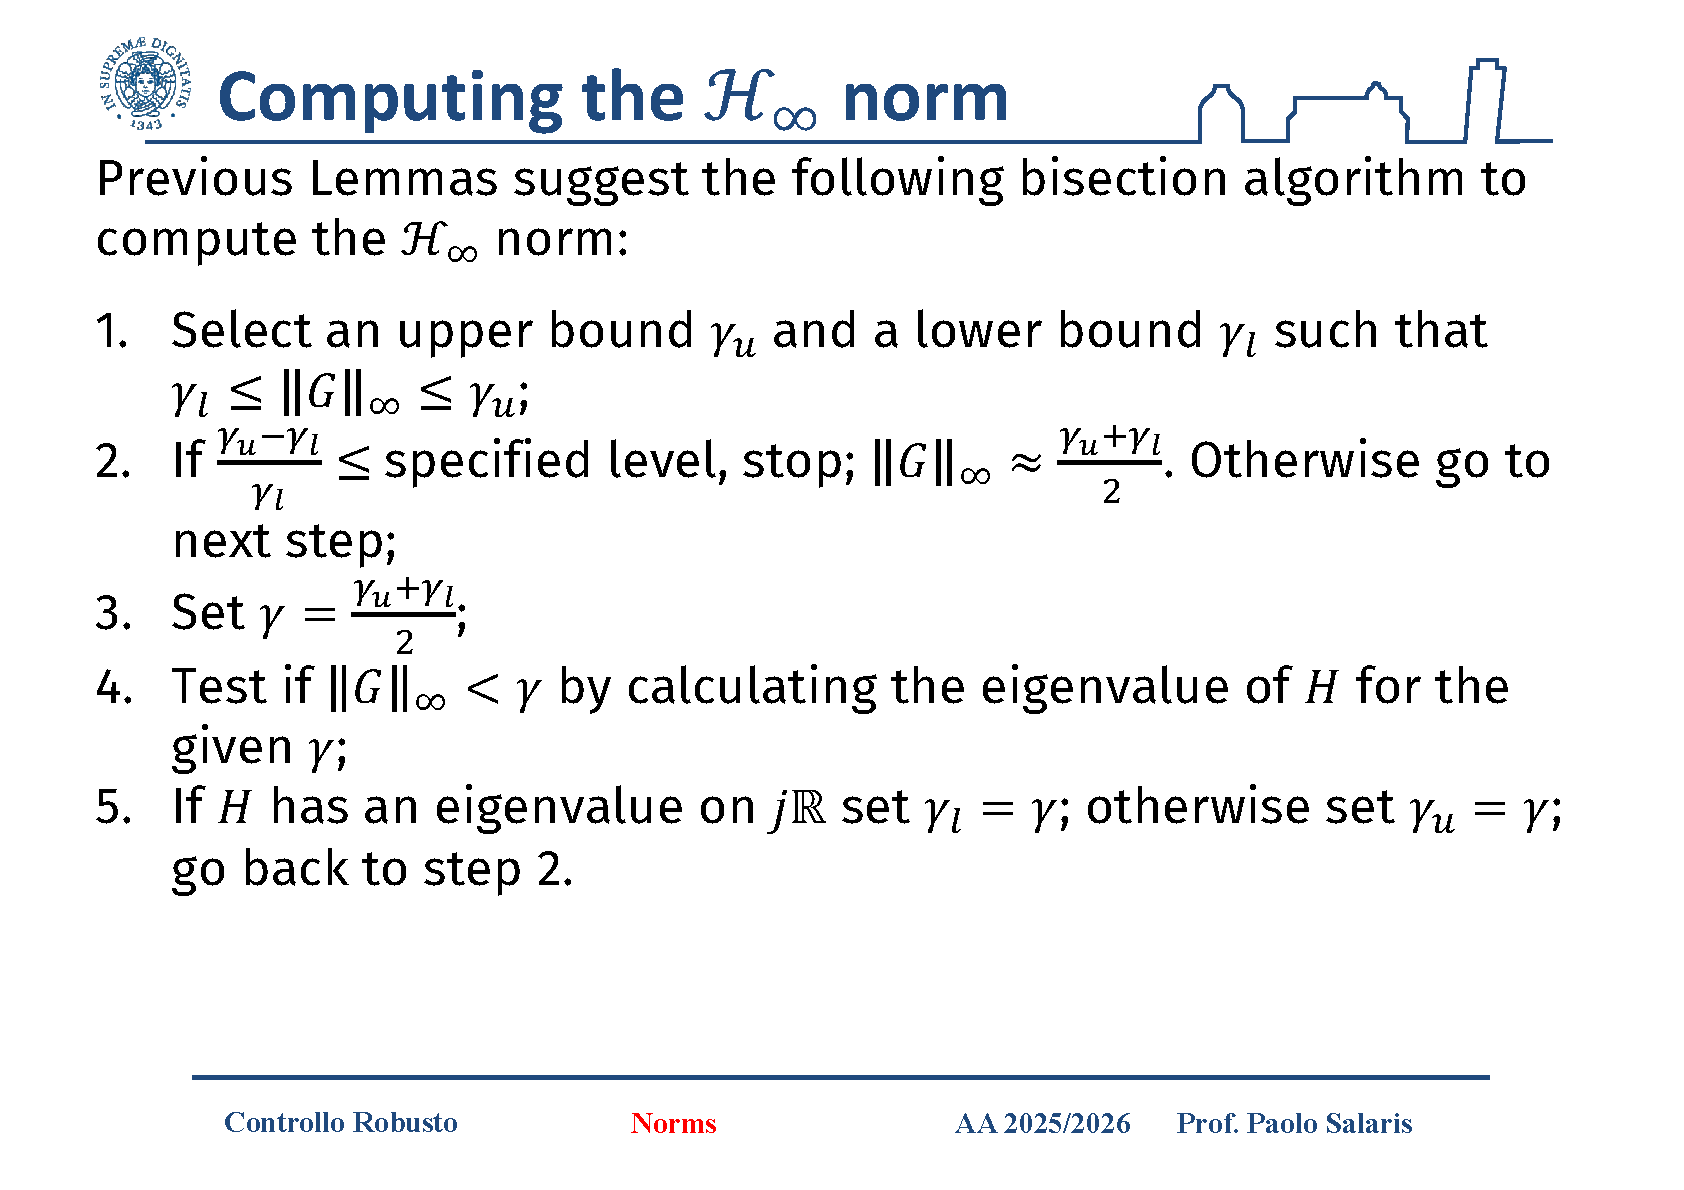
\includegraphics[width=0.82\textwidth]{images10/norms-new-60-76-001.png}
    \caption{Algoritmo per bisezione: la norma $H_\infty$ viene trovata cercando la soglia critica $\gamma$ in corrispondenza della quale la Hamiltoniana perde il certificato di bounded realness.}
\end{figure}

\subsection{Metodo di Routh--Hurwitz sul polinomio della Hamiltoniana}

La slide 61 propone un'alternativa utile quando la dimensione \`e piccola e il polinomio pu\`o essere manipolato a mano. Invece di calcolare gli autovalori di $\mathcal{H}_\gamma$, si considera il suo polinomio caratteristico
$$
\chi_\gamma(s)=\det(sI-\mathcal{H}_\gamma).
$$
Per una Hamiltoniana gli autovalori sono simmetrici rispetto all'origine: se $\lambda$ \`e autovalore, lo \`e anche $-\lambda$ con la struttura opportuna. Per questo, negli esempi delle slide, $\chi_\gamma(s)$ risulta pari:
$$
\chi_\gamma(s)=a_0s^{2n}+a_1s^{2n-2}+\cdots+a_n.
$$
Quando si costruisce la tabella di Routh di un polinomio pari, compare una riga di zeri. Non \`e un errore: \`e il caso speciale standard del criterio di Routh. Si prende il polinomio ausiliario associato alla riga precedente, lo si deriva rispetto a $s$, e si usano i coefficienti della derivata per sostituire la riga nulla.

La slide riassume poi il criterio nella forma pi\`u utile per il calcolo della norma. Sia $\{\gamma_i\}$ l'insieme dei valori $\gamma\ge0$ per cui un coefficiente dipendente da $\gamma$ nella prima colonna della tabella di Routh diventa zero. Tali valori sono soglie critiche: per essi il polinomio della Hamiltoniana ha radici sull'asse immaginario. La norma si ottiene prendendo la soglia critica pi\`u grande:
$$
\|G(s)\|_{H_\infty}=\sup_i\{\gamma_i\}.
$$
Questo punto \`e importante: non si prende il primo valore trovato, ma il massimo tra i valori critici, perch\'e la norma $H_\infty$ \`e il livello pi\`u alto raggiunto dalla curva dei valori singolari.

\begin{figure}[H]
    \centering
    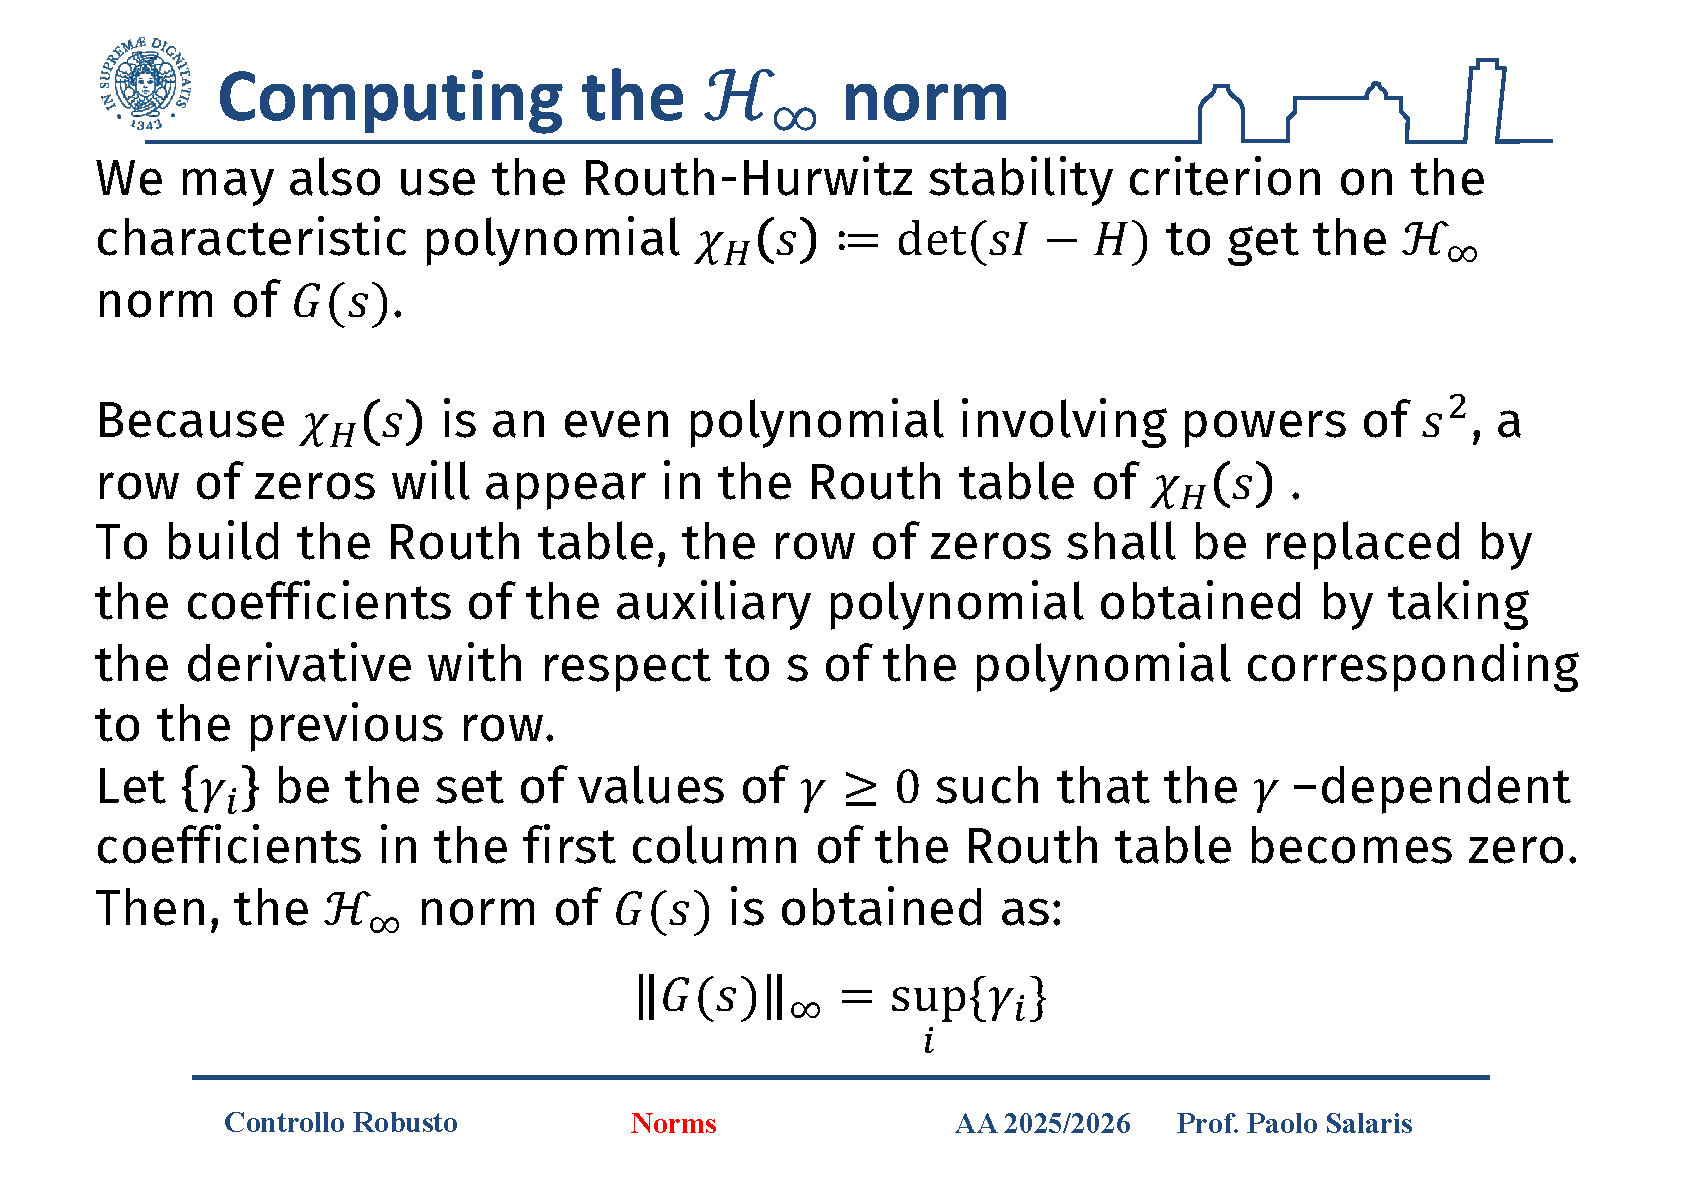
\includegraphics[width=0.82\textwidth]{images10/norms-new-60-76-002.png}
    \caption{Uso del criterio di Routh--Hurwitz: la norma $H_\infty$ si ricava dai valori di $\gamma$ che portano la Hamiltoniana ad avere autovalori sull'asse immaginario.}
\end{figure}

\subsection{Esempio scalare: \texorpdfstring{$G(s)=1/(s+2)$}{G(s)=1/(s+2)}}

Consideriamo
$$
G(s)=\frac{1}{s+2}.
$$
In questo caso il calcolo diretto \`e immediato:
$$
G(j\omega)=\frac{1}{2+j\omega},
\qquad
|G(j\omega)|=\frac{1}{\sqrt{4+\omega^2}}.
$$
Il massimo si ha in $\omega=0$, quindi
$$
\|G\|_{H_\infty}
=\sup_{\omega}|G(j\omega)|
=\frac{1}{2}.
$$

Usiamo ora il metodo Hamiltoniano. Una realizzazione minimale \`e
$$
A=-2,\qquad B=1,\qquad C=1,\qquad D=0.
$$
La Hamiltoniana strettamente propria \`e
$$
\mathcal{H}_\gamma=
\begin{bmatrix}
-2 & \gamma^{-2}\\
-1 & 2
\end{bmatrix}.
$$
Il suo polinomio caratteristico \`e
$$
\chi_\gamma(s)=\det(sI-\mathcal{H}_\gamma)
=
\det
\begin{bmatrix}
s+2 & -\gamma^{-2}\\
1 & s-2
\end{bmatrix}
=s^2-4+\gamma^{-2}.
$$
La tabella di Routh contiene una riga nulla perch\'e il polinomio \`e pari. Il polinomio ausiliario \`e
$$
s^2-4+\gamma^{-2},
$$
e la sua derivata \`e
$$
\frac{d}{ds}\left(s^2-4+\gamma^{-2}\right)=2s.
$$
Il valore critico si ottiene imponendo
$$
-4+\gamma^{-2}=0,
$$
cio\`e
$$
\gamma=\frac{1}{2}.
$$
Il metodo Hamiltoniano/Routh restituisce quindi lo stesso risultato del calcolo diretto.

\begin{figure}[H]
    \centering
    \begin{subfigure}{0.48\textwidth}
        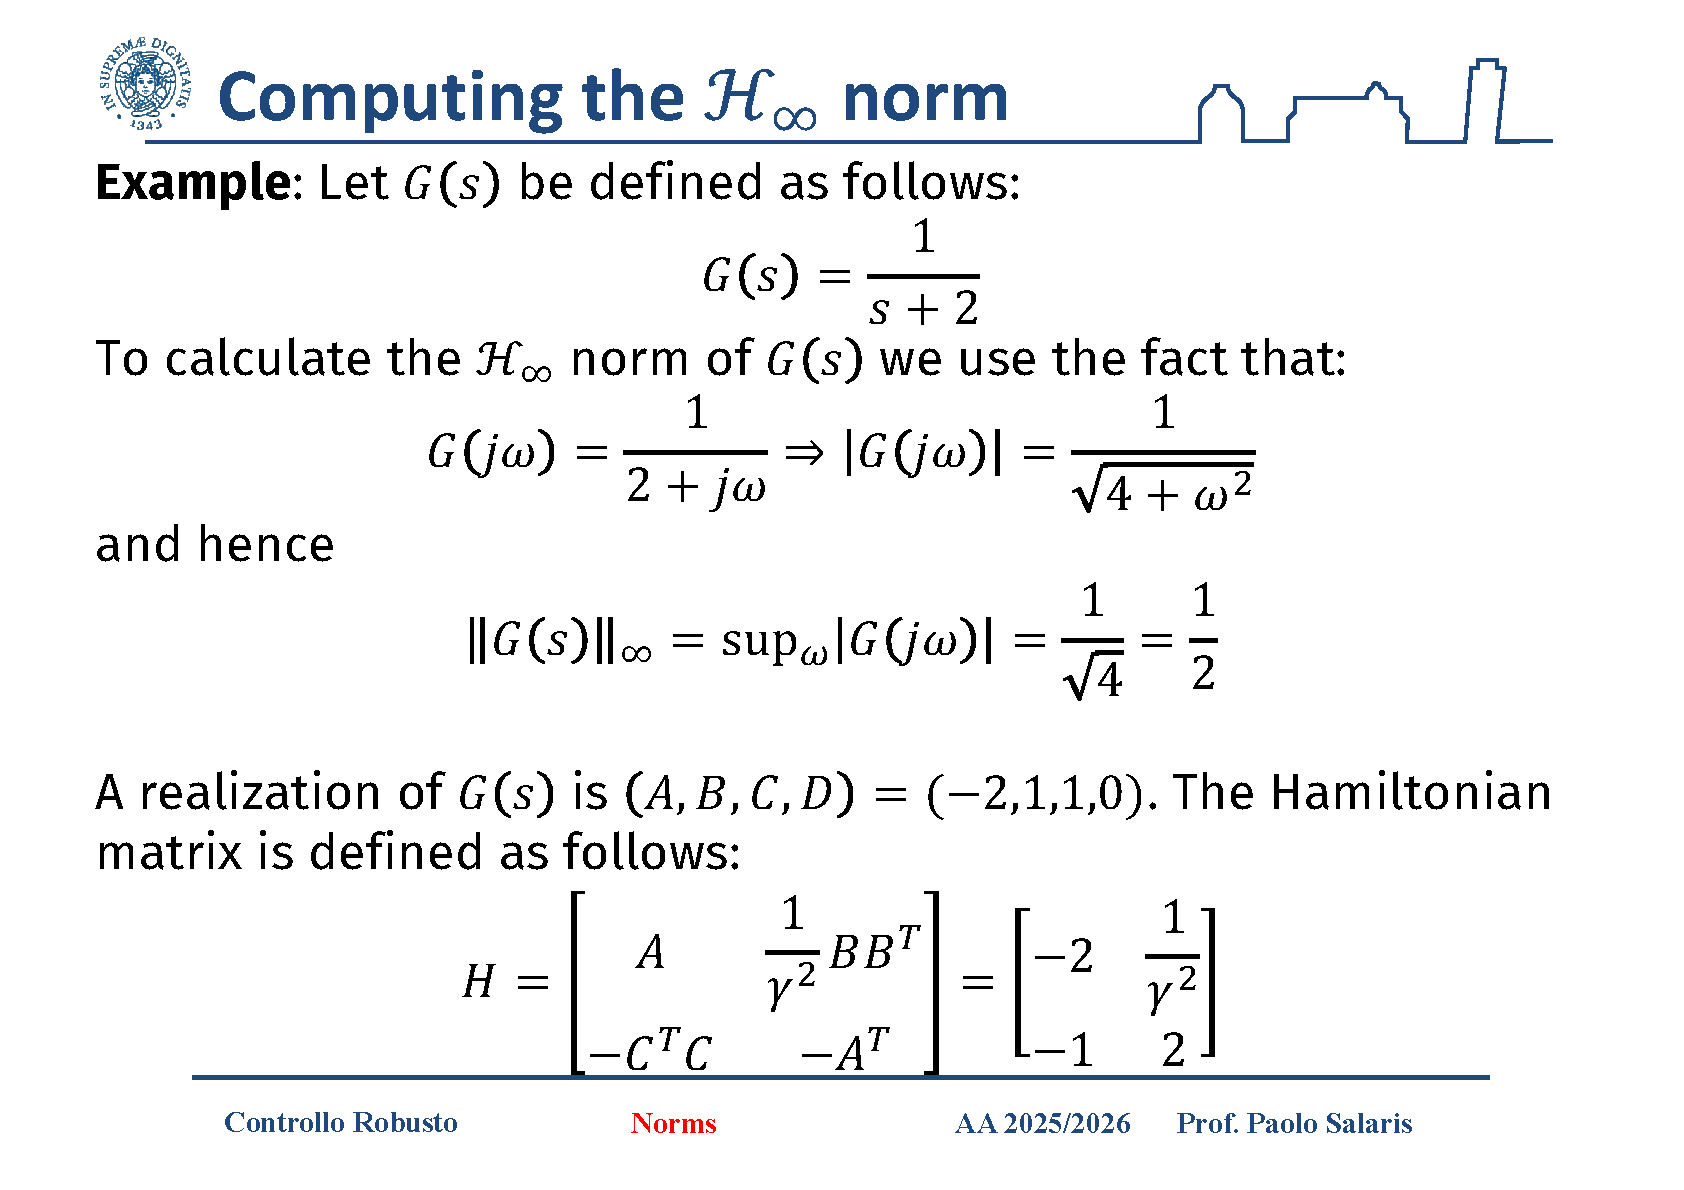
\includegraphics[width=\linewidth]{images10/norms-new-60-76-003.png}
        \caption{Calcolo diretto e costruzione della Hamiltoniana per $G(s)=1/(s+2)$.}
    \end{subfigure}
    \hfill
    \begin{subfigure}{0.48\textwidth}
        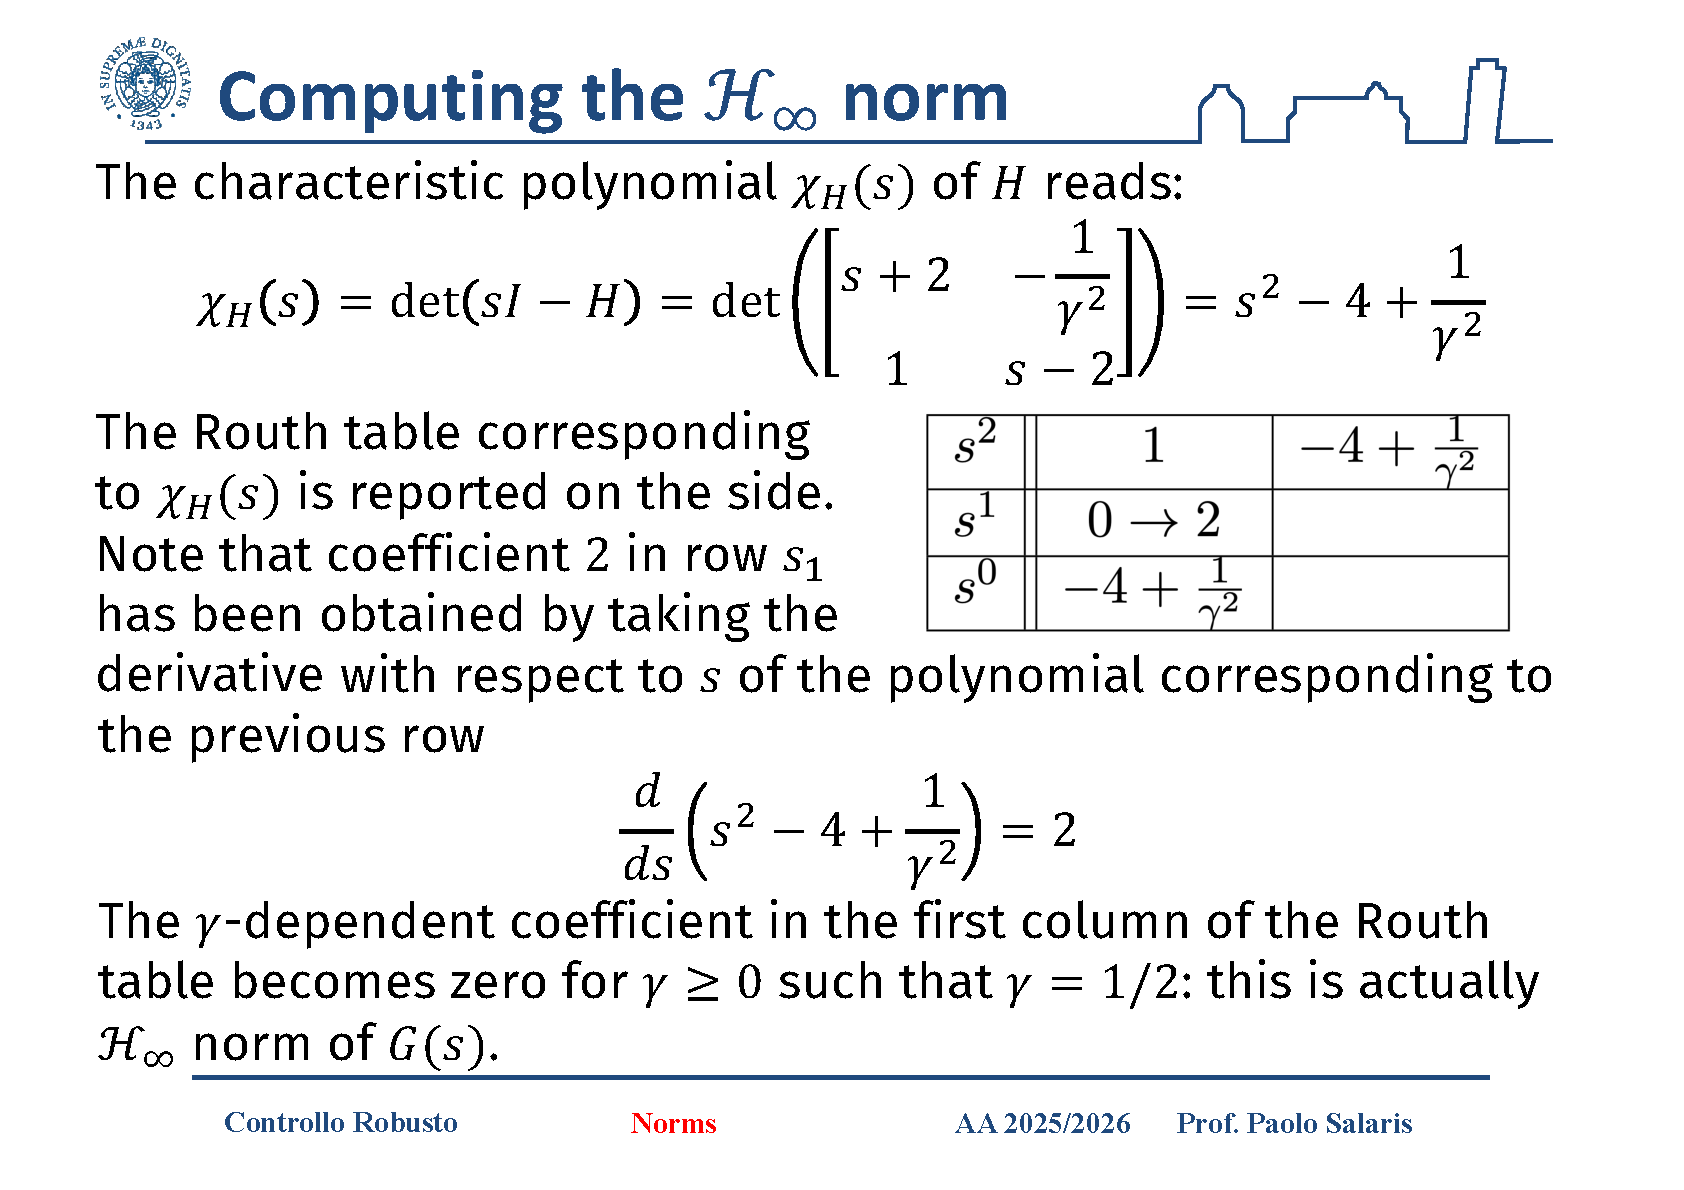
\includegraphics[width=\linewidth]{images10/norms-new-60-76-004.png}
        \caption{Tabella di Routh e valore critico $\gamma=1/2$.}
    \end{subfigure}
    \caption{Nel caso scalare la norma $H_\infty$ pu\`o essere letta direttamente dal diagramma di Bode oppure ricavata dal polinomio della Hamiltoniana.}
\end{figure}

\subsection{Esempio vettoriale: due canali di uscita}

Il secondo esempio considera
$$
G(s)=
\begin{bmatrix}
\dfrac{1}{s+1}\\[0.7em]
\dfrac{1}{s+2}
\end{bmatrix}.
$$
Poich\'e il sistema ha un solo ingresso e due uscite, $G(j\omega)$ \`e un vettore colonna. Il suo massimo valore singolare \`e la norma euclidea del vettore:
$$
\bar{\sigma}(G(j\omega))
=
\sqrt{
\frac{1}{\omega^2+1}
+
\frac{1}{\omega^2+4}
}.
$$
La funzione \`e decrescente in $\omega^2$, quindi il massimo si ha a $\omega=0$:
$$
\|G\|_{H_\infty}
=
\sqrt{1+\frac{1}{4}}
=\frac{\sqrt{5}}{2}.
$$

La slide mostra anche il calcolo tramite valori singolari. Poich\'e $G(j\omega)$ \`e una colonna, il prodotto $G^H(j\omega)G(j\omega)$ \`e uno scalare:
$$
G^H(j\omega)G(j\omega)
=
\frac{1}{\omega^2+1}+\frac{1}{\omega^2+4}
=
\frac{2\omega^2+5}{(\omega^2+1)(\omega^2+4)}.
$$
Il prodotto opposto $G(j\omega)G^H(j\omega)$ \`e invece una matrice $2\times2$ di rango uno. I due prodotti hanno gli stessi autovalori non nulli, quindi l'unico autovalore non nullo di $G(j\omega)G^H(j\omega)$ \`e
$$
\lambda(\omega)=
\frac{2\omega^2+5}{(\omega^2+1)(\omega^2+4)},
$$
e
$$
\bar{\sigma}(G(j\omega))=\sqrt{\lambda(\omega)}.
$$

\begin{figure}[H]
    \centering
    \begin{subfigure}{0.48\textwidth}
        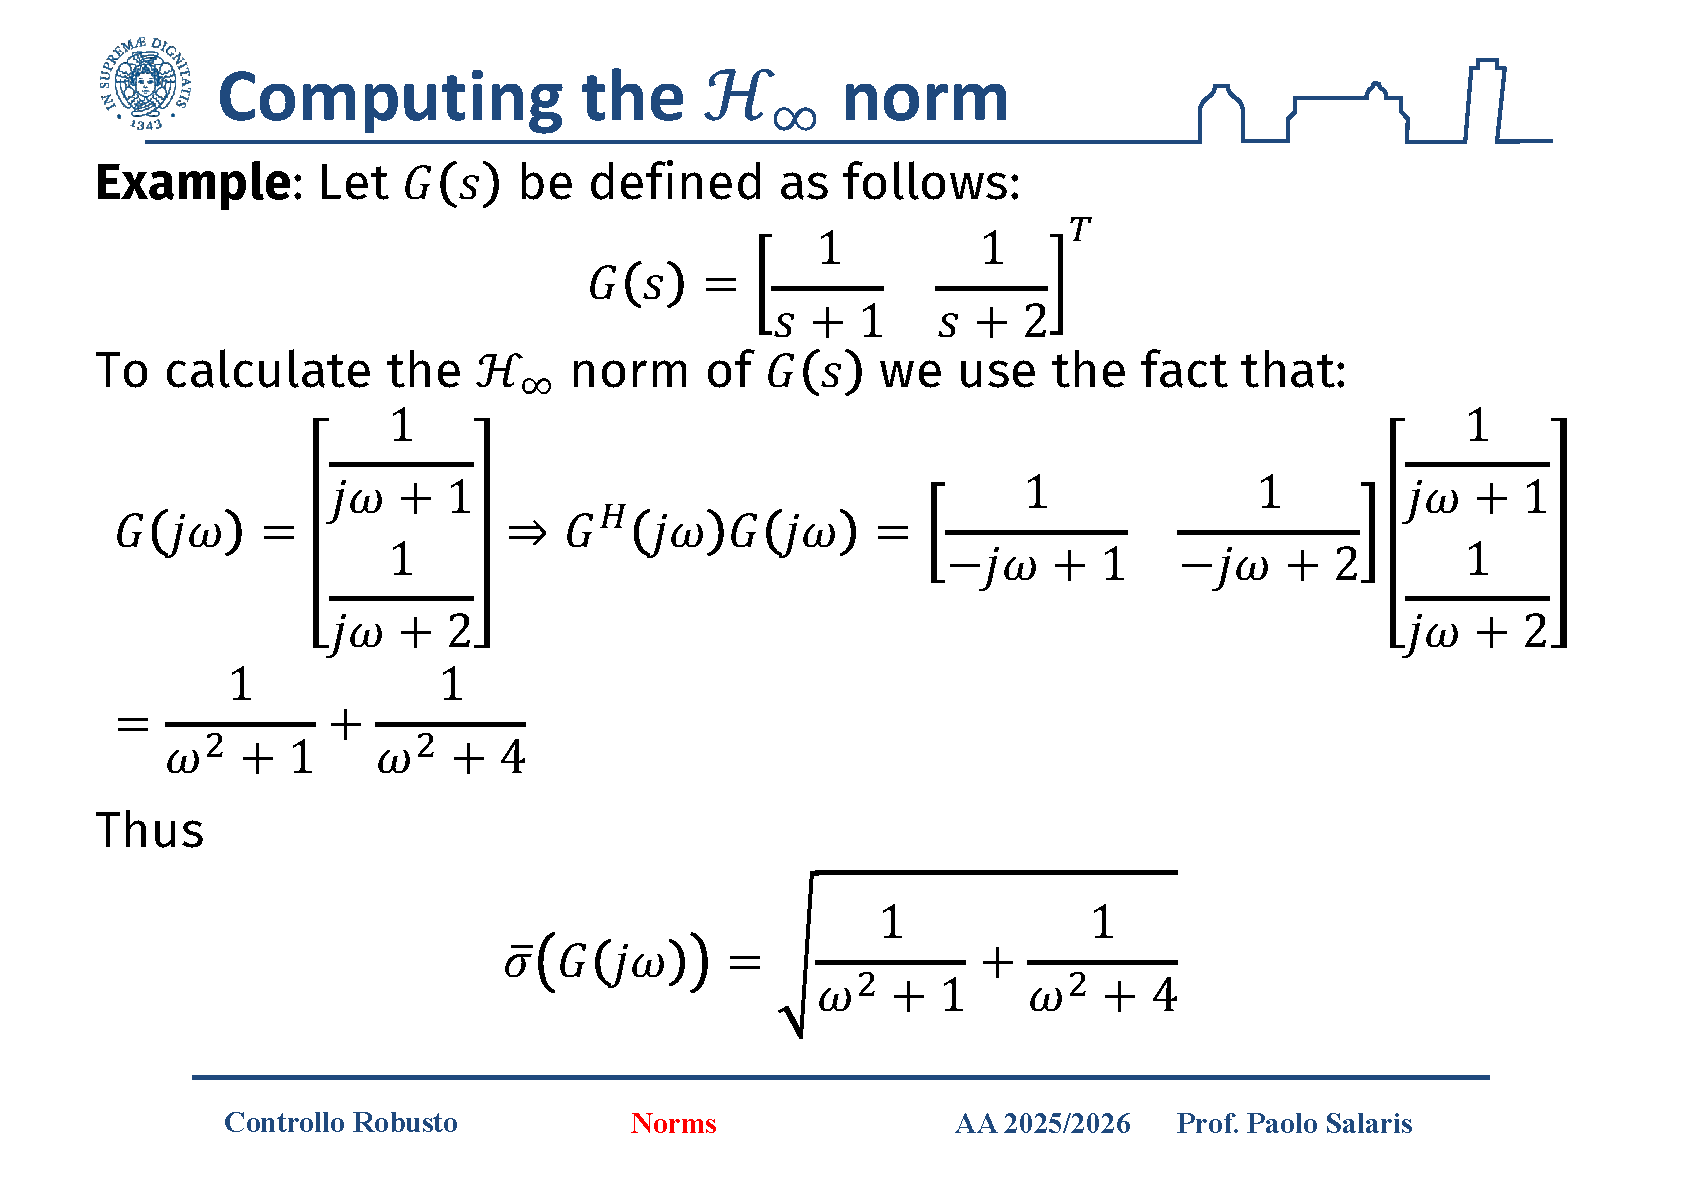
\includegraphics[width=\linewidth]{images10/norms-new-60-76-005.png}
        \caption{Calcolo diretto della norma tramite $G^H(j\omega)G(j\omega)$.}
    \end{subfigure}
    \hfill
    \begin{subfigure}{0.48\textwidth}
        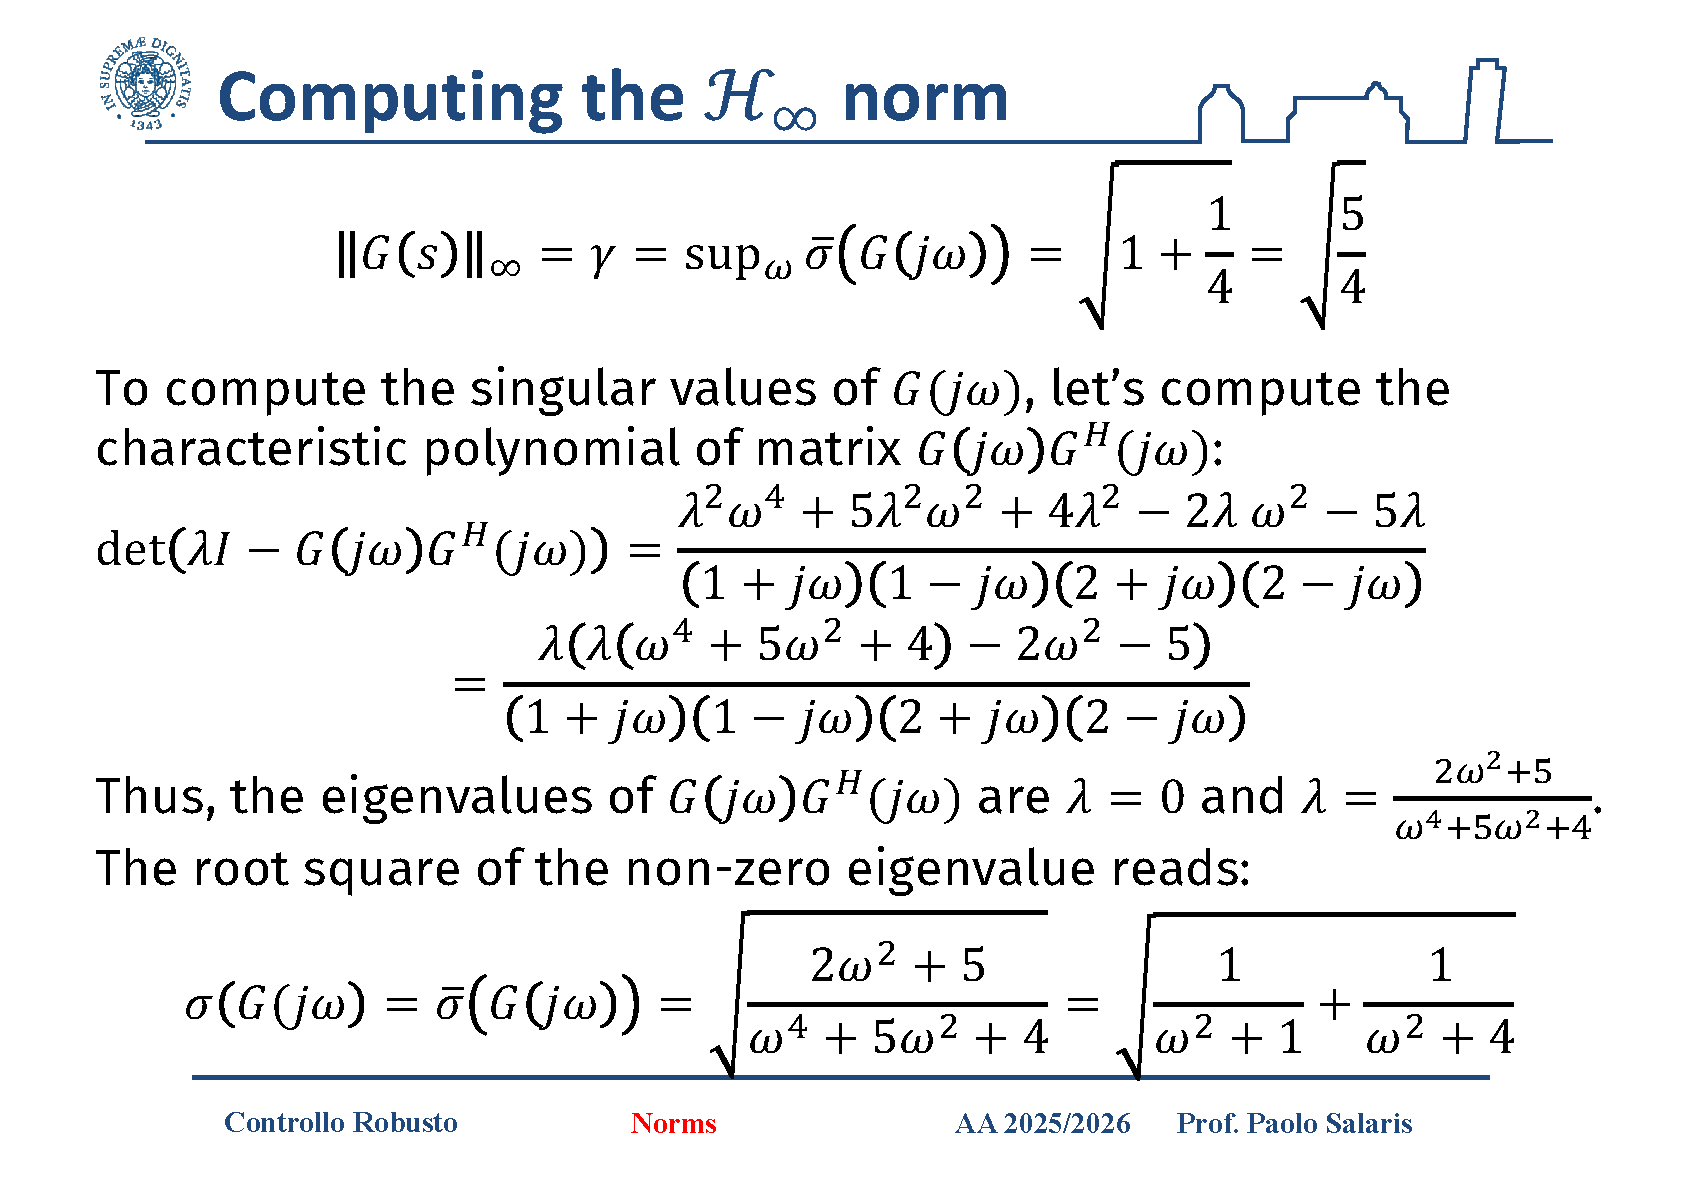
\includegraphics[width=\linewidth]{images10/norms-new-60-76-006.png}
        \caption{Autovalori di $G(j\omega)G^H(j\omega)$ e massimo valore singolare.}
    \end{subfigure}
    \caption{Per un sistema con un solo ingresso, il massimo valore singolare coincide con la norma euclidea della colonna di trasferimenti.}
\end{figure}

Una realizzazione usata nelle slide \`e
$$
A=
\begin{bmatrix}
0 & 1\\
-2 & -3
\end{bmatrix},
\qquad
B=
\begin{bmatrix}
0\\
1
\end{bmatrix},
\qquad
C=
\begin{bmatrix}
2 & 1\\
1 & 1
\end{bmatrix},
\qquad
D=0.
$$
La Hamiltoniana associata \`e
$$
\mathcal{H}_\gamma=
\begin{bmatrix}
A & \gamma^{-2}BB^T\\
-C^TC & -A^T
\end{bmatrix}
=
\begin{bmatrix}
0 & 1 & 0 & 0\\
-2 & -3 & 0 & \gamma^{-2}\\
-5 & -3 & 0 & 2\\
-3 & -2 & -1 & 3
\end{bmatrix}.
$$
Il polinomio caratteristico \`e
$$
\chi_\gamma(s)
=
s^4+\left(\frac{2}{\gamma^2}-5\right)s^2
+4-\frac{5}{\gamma^2}.
$$
Applicando Routh--Hurwitz e sostituendo la riga nulla con la derivata del polinomio ausiliario, le voci dipendenti da $\gamma$ nella prima colonna sono proporzionali a
$$
\frac{2}{\gamma^2}-5,
\qquad
\frac{88}{\gamma^2}-84,
\qquad
4-\frac{5}{\gamma^2}.
$$
Annullandole si ottiene
$$
\gamma\in
\left\{
\sqrt{\frac{2}{5}},
\sqrt{\frac{88}{84}},
\sqrt{\frac{5}{4}}
\right\}.
$$
La norma $H_\infty$ \`e il massimo fra questi valori:
$$
\|G\|_{H_\infty}
=
\sup_i\{\gamma_i\}
=
\sqrt{\frac{5}{4}}
=
\frac{\sqrt{5}}{2}.
$$

\begin{figure}[H]
    \centering
    \begin{subfigure}{0.48\textwidth}
        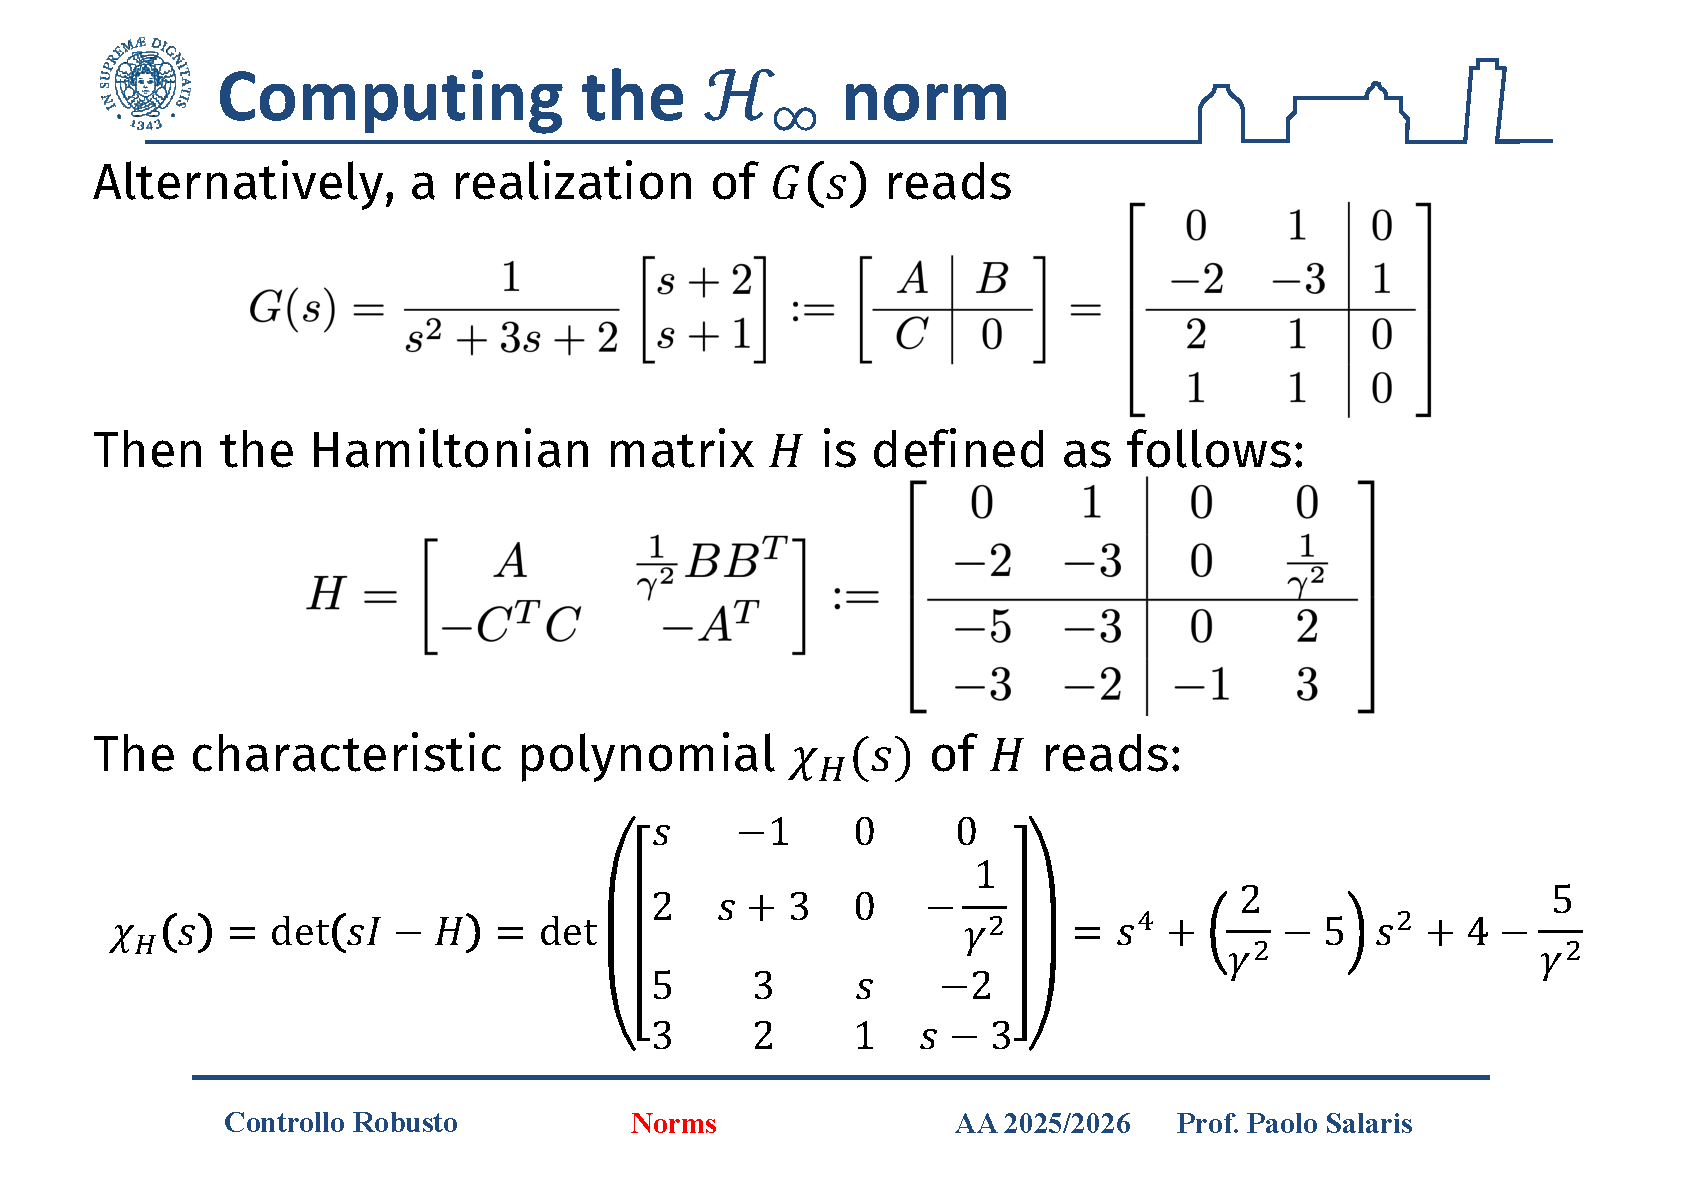
\includegraphics[width=\linewidth]{images10/norms-new-60-76-007.png}
        \caption{Realizzazione di stato, Hamiltoniana e polinomio caratteristico.}
    \end{subfigure}
    \hfill
    \begin{subfigure}{0.48\textwidth}
        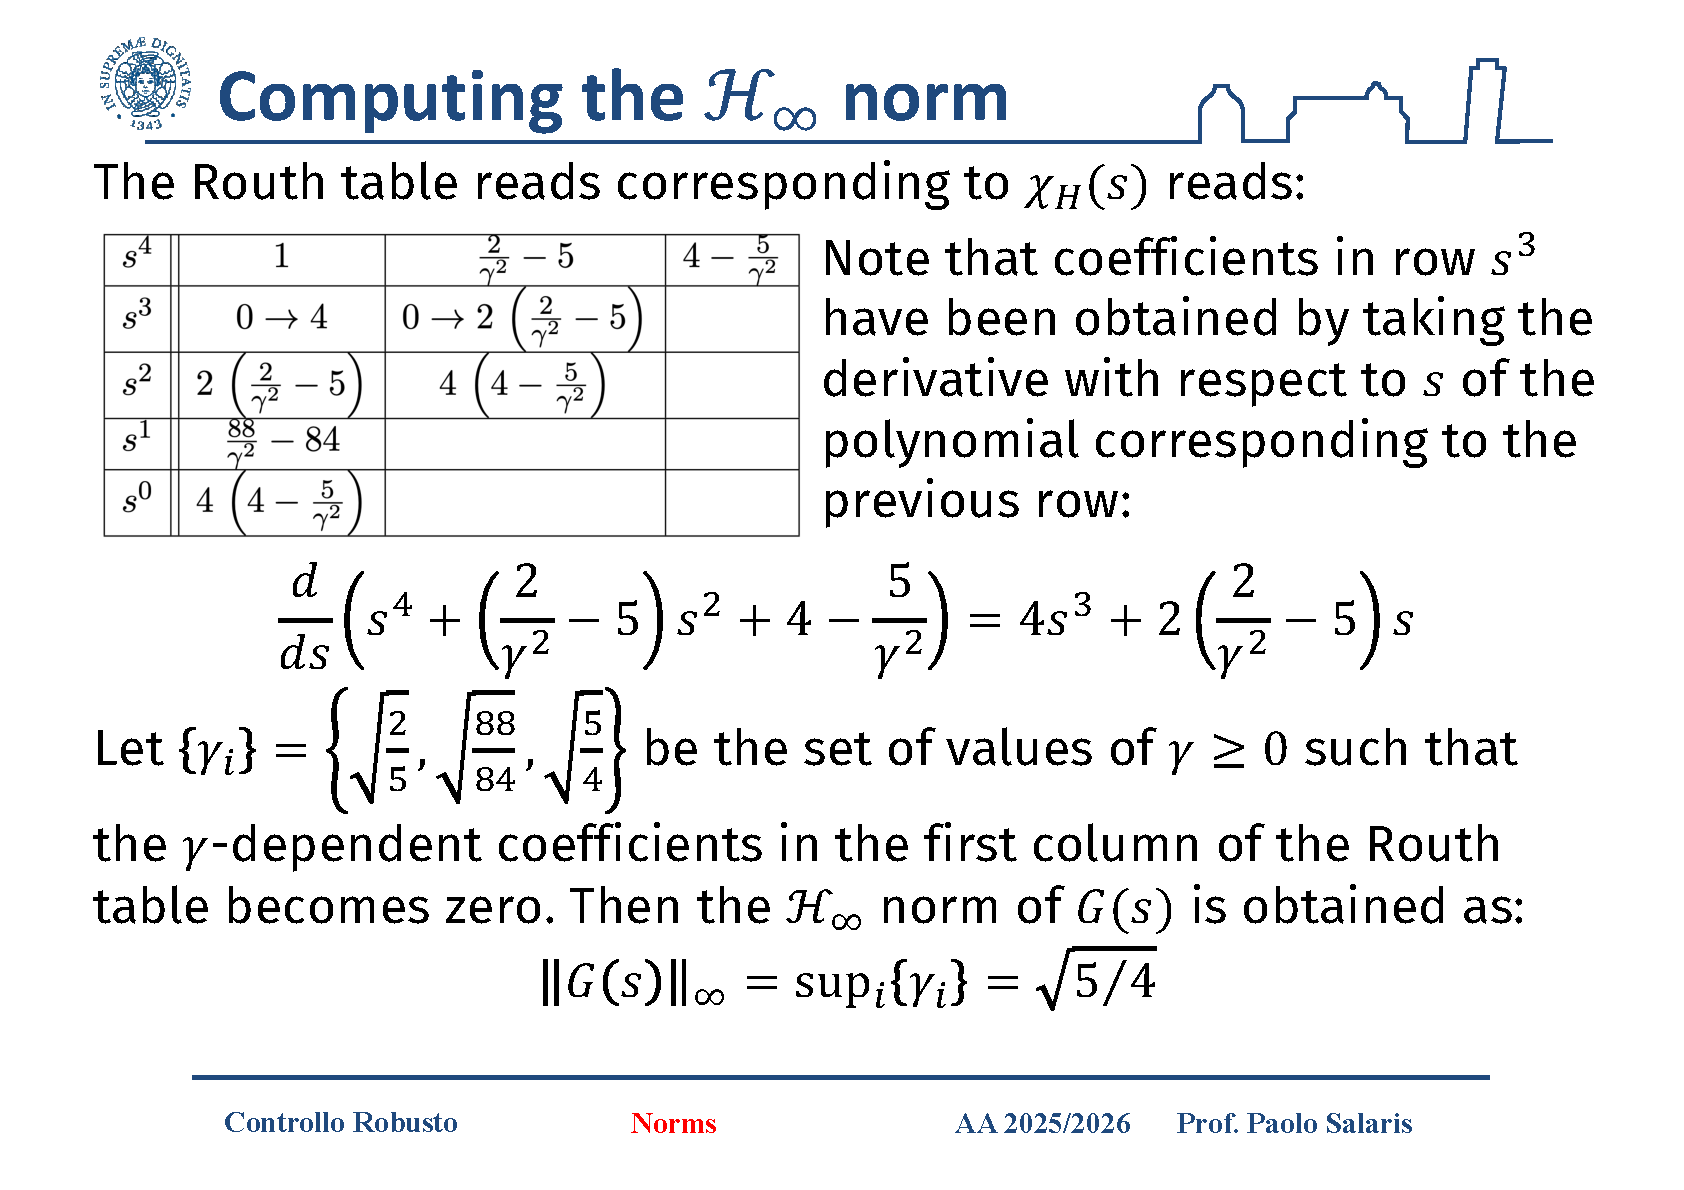
\includegraphics[width=\linewidth]{images10/norms-new-60-76-008.png}
        \caption{Tabella di Routh e selezione del valore critico pi\`u grande.}
    \end{subfigure}
    \caption{L'esempio mostra che il metodo di Routh produce gli stessi valori critici che delimitano la norma $H_\infty$.}
\end{figure}

\subsection{Esempio scalare generale e legame con Riccati}

Consideriamo ora
$$
g(s)=\frac{1}{s-a},
\qquad
a<0,
$$
con realizzazione
$$
(A,B,C,D)=(a,1,1,0).
$$
Il risultato atteso, guardando direttamente la risposta in frequenza, \`e
$$
\|g\|_{H_\infty}
=
\sup_\omega\frac{1}{|j\omega-a|}
=
\frac{1}{|a|},
$$
perch\'e il denominatore \`e minimo in $\omega=0$. La slide usa questo esempio per mostrare che la stessa soglia emerge anche dalla Riccati e dalla Hamiltoniana.

La Riccati del bounded real lemma diventa
$$
2ap+\frac{p^2}{\gamma^2}+1=0.
$$
Le soluzioni sono
$$
p=\gamma^2\left(-a\pm\sqrt{a^2-\gamma^{-2}}\right).
$$
La dinamica chiusa associata alla soluzione \`e
$$
a+\frac{p}{\gamma^2}
=
\pm\sqrt{a^2-\gamma^{-2}}.
$$
Per avere una soluzione stabilizzante, questa quantit\`a deve essere reale e negativa; dunque bisogna scegliere il segno meno e richiedere
$$
a^2-\gamma^{-2}>0.
$$
Poich\'e $a<0$, questo equivale a
$$
\gamma>\frac{1}{|a|}.
$$
Ne segue
$$
\|g\|_{H_\infty}
=
\inf\left\{\gamma:\|g\|_{H_\infty}<\gamma\right\}
=
\frac{1}{|a|}.
$$

Lo stesso risultato si vede dalla Hamiltoniana
$$
\mathcal{H}_\gamma=
\begin{bmatrix}
a & \gamma^{-2}\\
-1 & -a
\end{bmatrix},
$$
i cui autovalori sono
$$
\lambda(\mathcal{H}_\gamma)
=
\pm\sqrt{a^2-\gamma^{-2}}.
$$
La Hamiltoniana non ha autovalori immaginari se e solo se
$$
\gamma>\frac{1}{|a|}.
$$

\begin{figure}[H]
    \centering
    \begin{subfigure}{0.48\textwidth}
        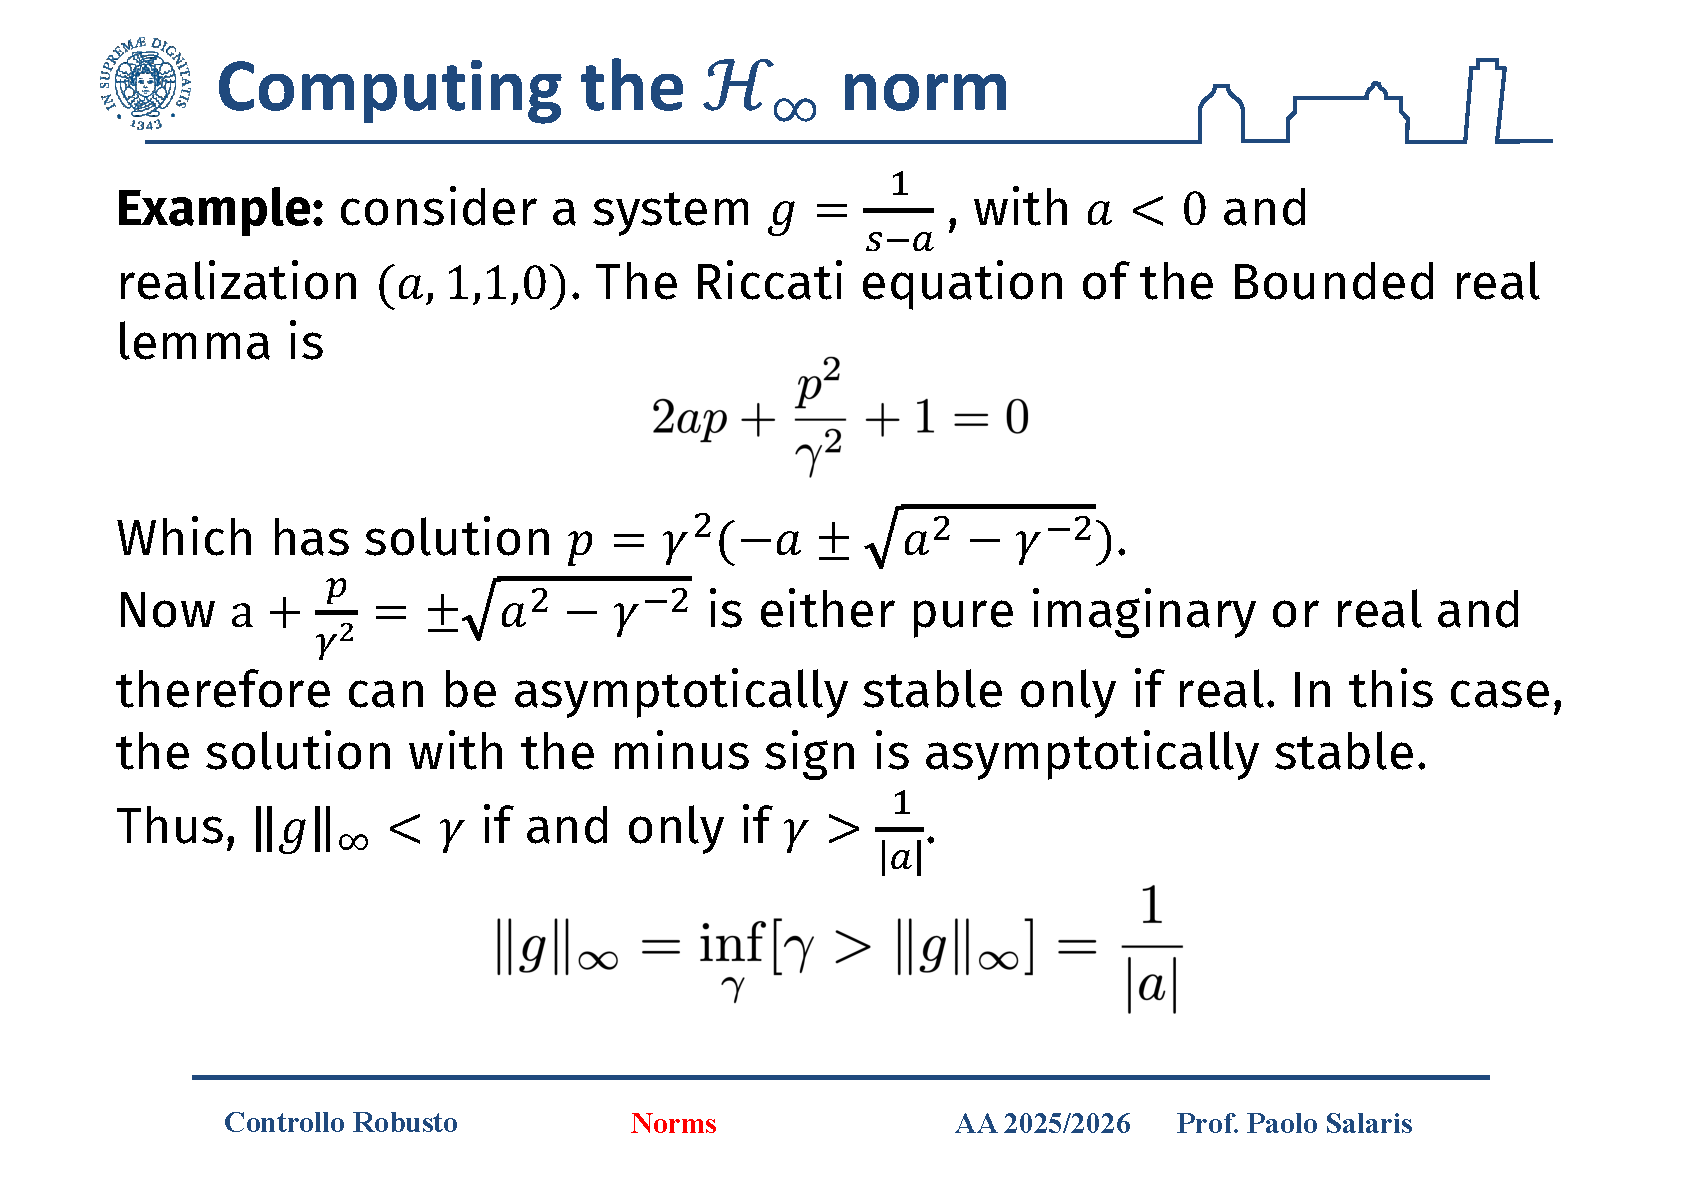
\includegraphics[width=\linewidth]{images10/norms-new-60-76-009.png}
        \caption{Riccati scalare e condizione sulla soluzione stabilizzante.}
    \end{subfigure}
    \hfill
    \begin{subfigure}{0.48\textwidth}
        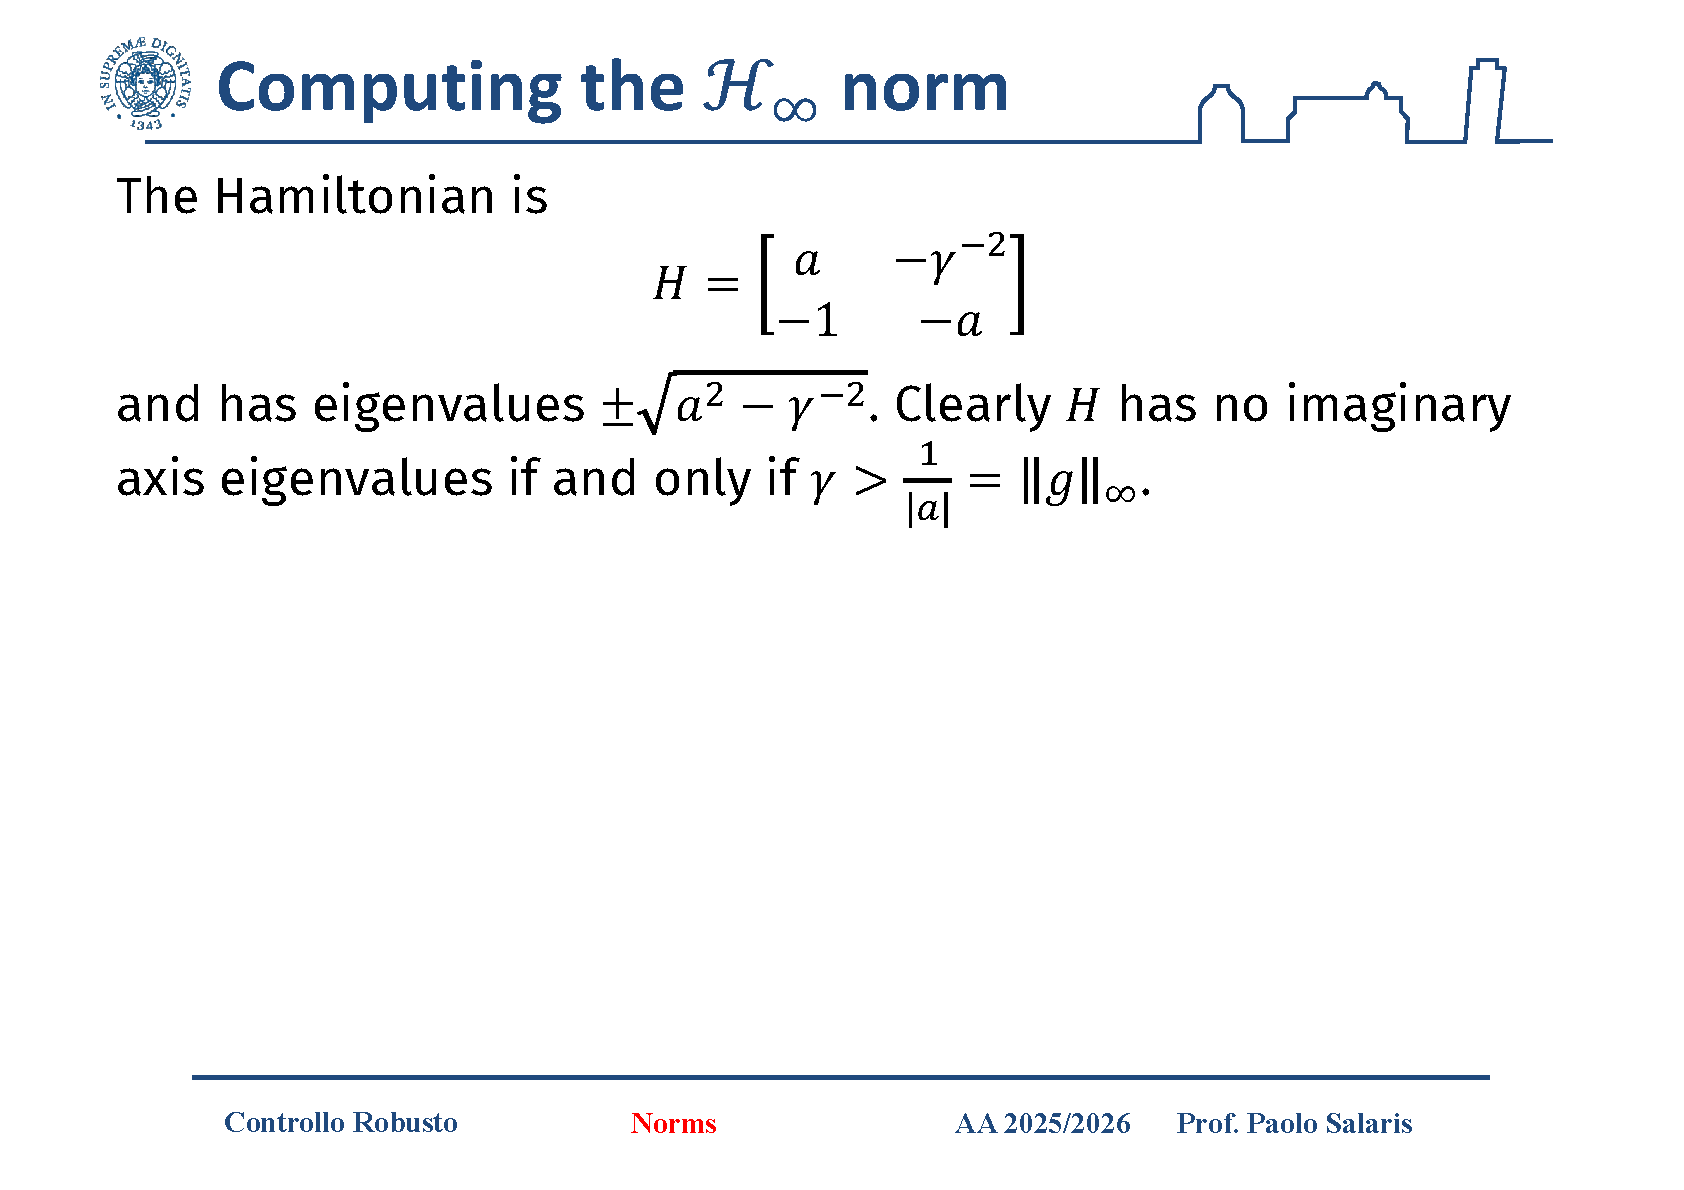
\includegraphics[width=\linewidth]{images10/norms-new-60-76-010.png}
        \caption{La stessa soglia emerge dagli autovalori della Hamiltoniana.}
    \end{subfigure}
    \caption{Nel primo ordine scalare, Riccati e Hamiltoniana danno in modo trasparente $\|g\|_{H_\infty}=1/|a|$.}
\end{figure}

\subsection{Confronto tra norme \texorpdfstring{$H_\infty$}{H-infinito} e \texorpdfstring{$H_2$}{H2}}

Le slide riassumono il confronto con due frasi molto efficaci:
\begin{itemize}
    \item $H_\infty$ spinge verso il basso il picco del massimo valore singolare;
    \item $H_2$ spinge verso il basso l'intera risposta, cio\`e l'energia distribuita su tutte le frequenze.
\end{itemize}

Per il sistema stabile
$$
G(s)=\frac{1}{s+a},
\qquad
a>0,
$$
la norma $H_\infty$ \`e
$$
\|G\|_{H_\infty}
=
\max_\omega |G(j\omega)|
=
\max_\omega \frac{1}{\sqrt{\omega^2+a^2}}
=
\frac{1}{a}.
$$
La norma $H_2$ invece \`e
$$
\|G\|_{H_2}
=
\left(
\frac{1}{2\pi}
\int_{-\infty}^{+\infty}
|G(j\omega)|^2\,d\omega
\right)^{1/2}
=
\left(
\frac{1}{2\pi}
\int_{-\infty}^{+\infty}
\frac{1}{\omega^2+a^2}\,d\omega
\right)^{1/2}.
$$
Usando
$$
\int_{-\infty}^{+\infty}
\frac{1}{\omega^2+a^2}\,d\omega
=
\frac{\pi}{a},
$$
si ottiene
$$
\|G\|_{H_2}
=
\sqrt{\frac{1}{2a}}.
$$

Lo stesso risultato segue nel dominio del tempo. La risposta impulsiva \`e
$$
g(t)=\mathcal{L}^{-1}\left\{\frac{1}{s+a}\right\}=e^{-at},
\qquad
t\ge 0.
$$
Quindi
$$
\|g\|_{L_2}
=
\left(
\int_0^\infty e^{-2at}\,dt
\right)^{1/2}
=
\sqrt{\frac{1}{2a}},
$$
in accordo con Parseval.

\begin{figure}[H]
    \centering
    \begin{subfigure}{0.48\textwidth}
        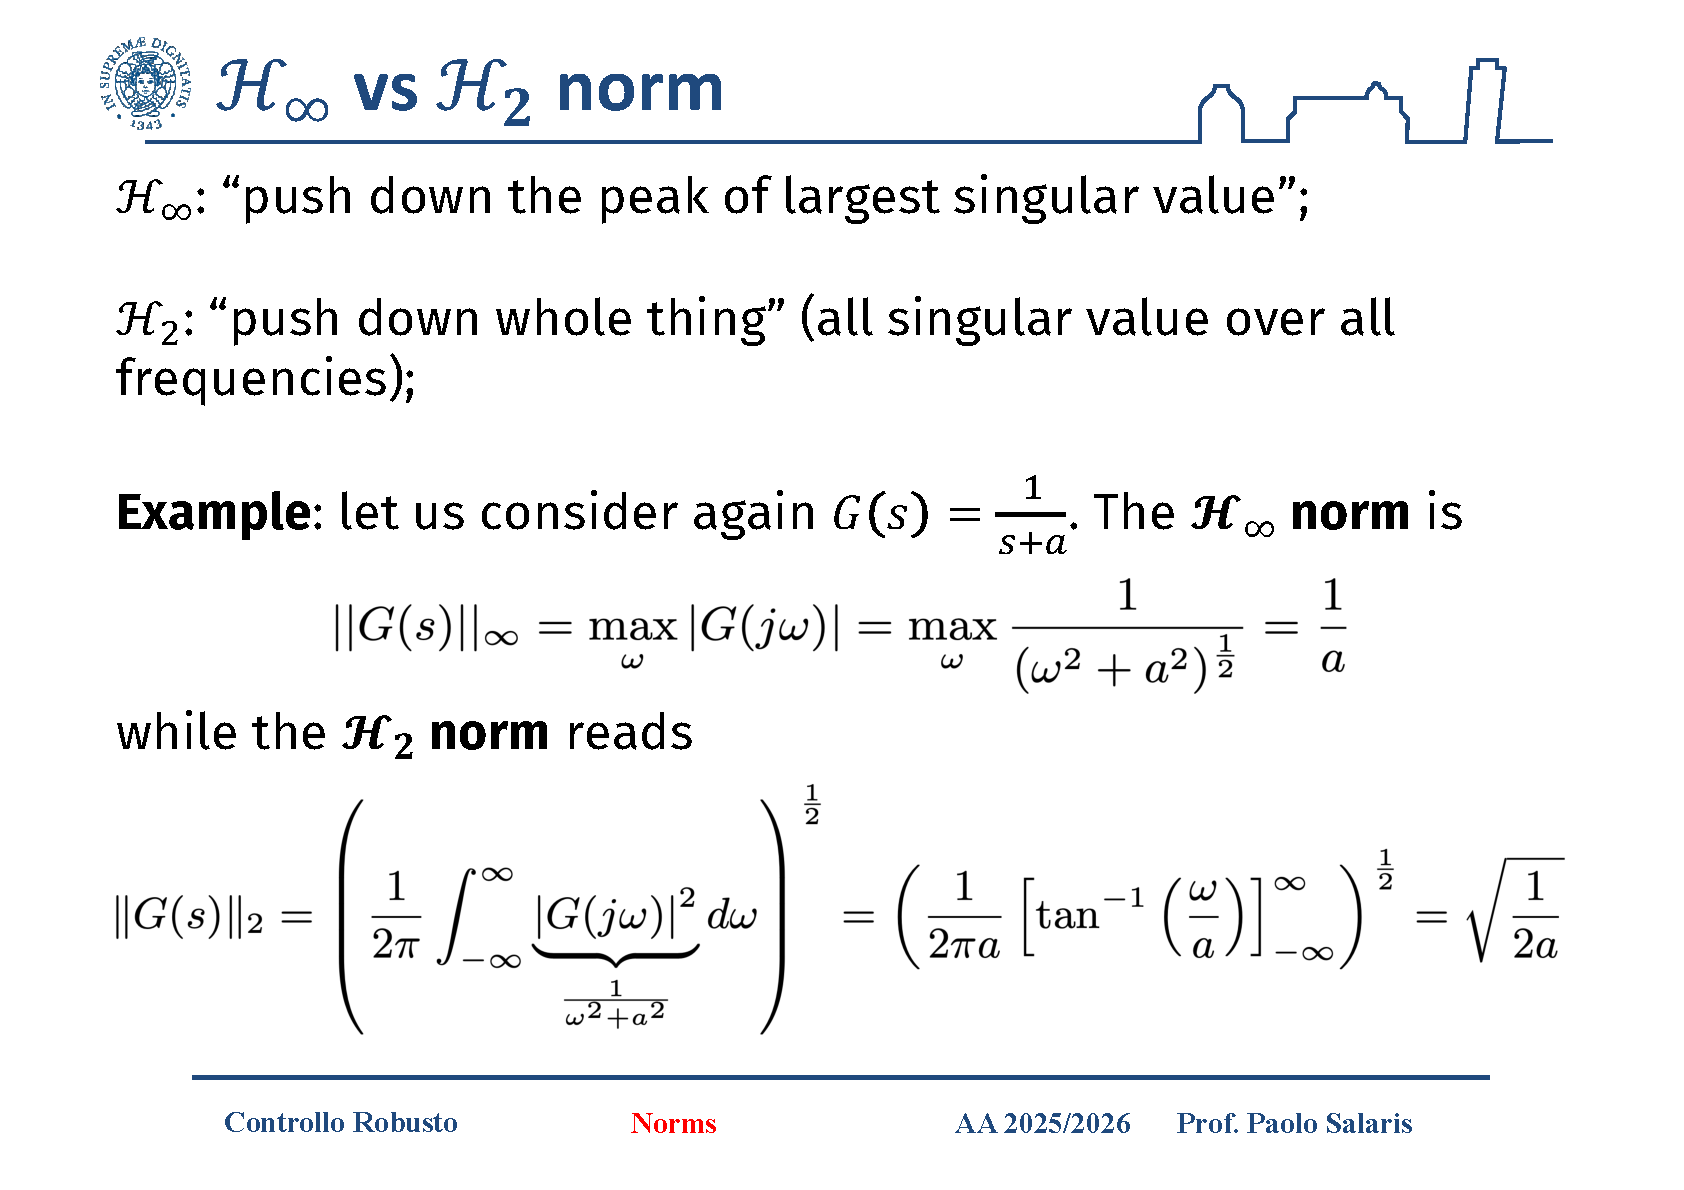
\includegraphics[width=\linewidth]{images10/norms-new-60-76-011.png}
        \caption{La norma $H_\infty$ misura il picco, mentre la norma $H_2$ misura l'energia complessiva.}
    \end{subfigure}
    \hfill
    \begin{subfigure}{0.48\textwidth}
        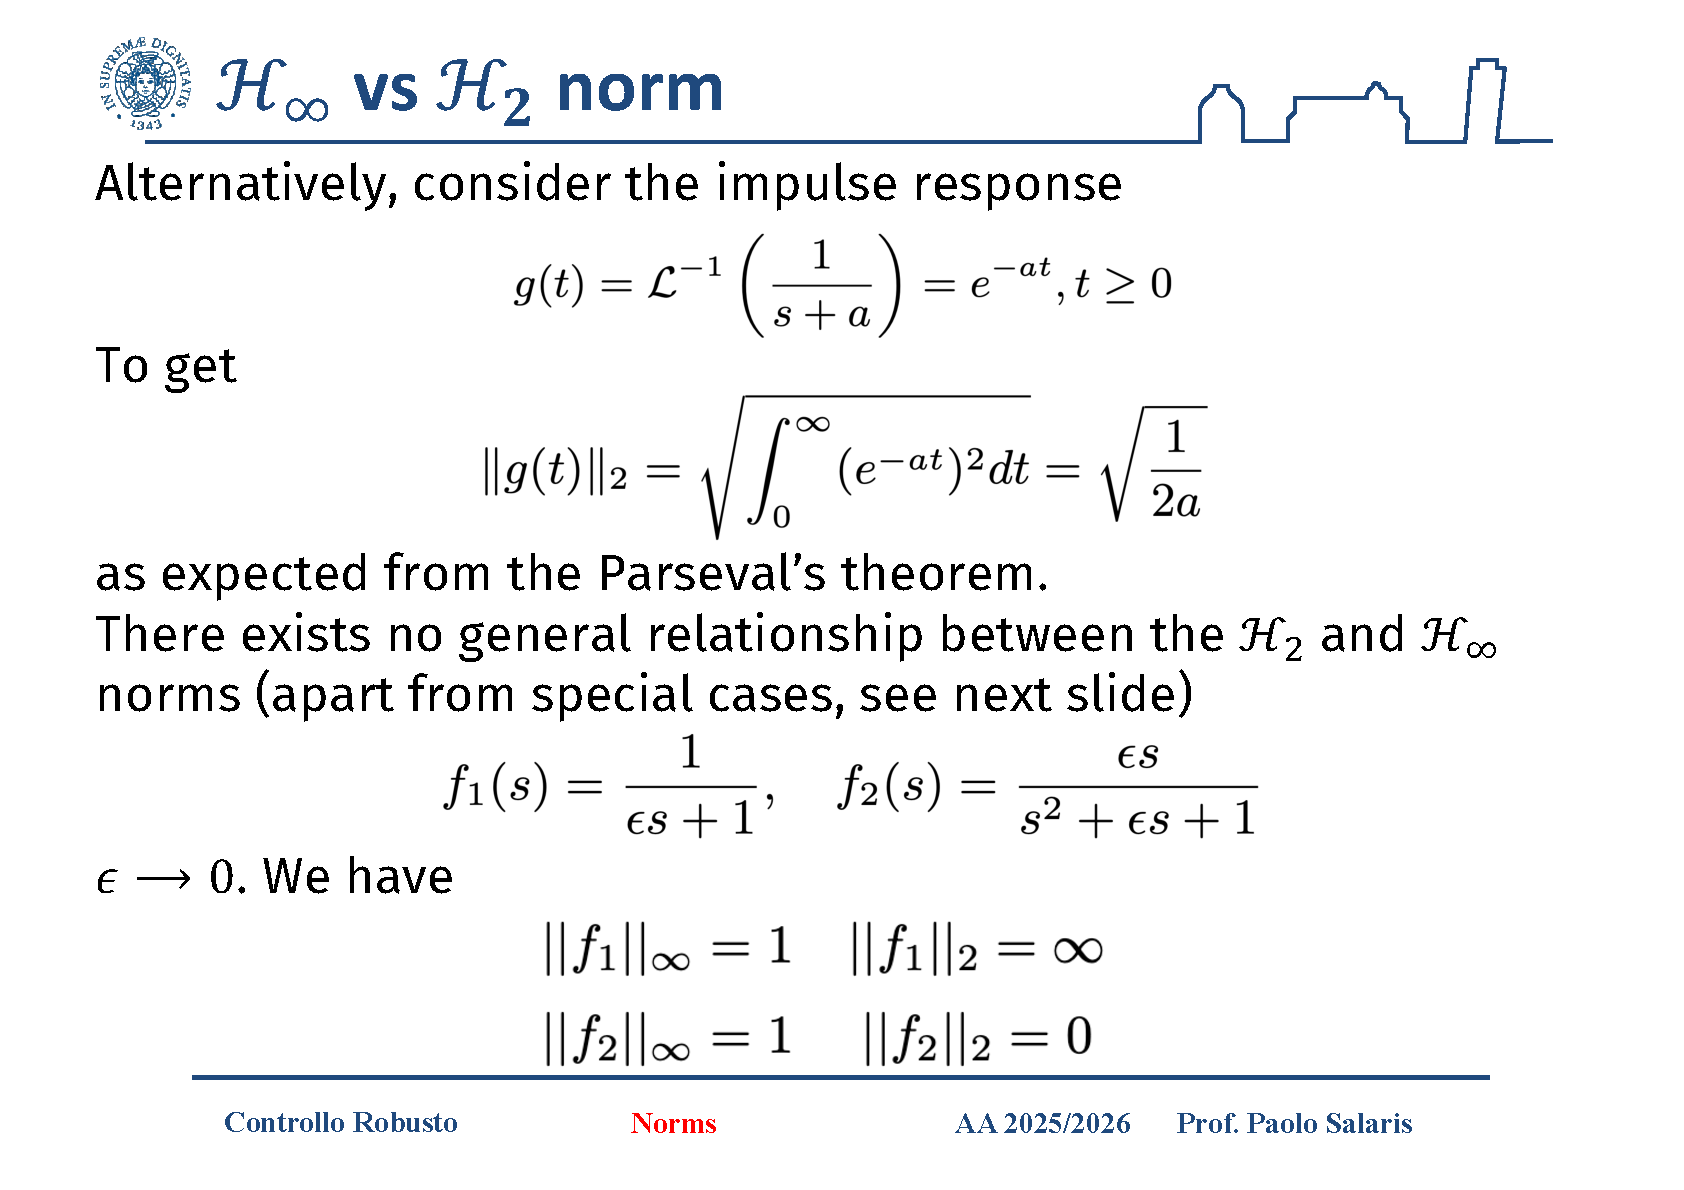
\includegraphics[width=\linewidth]{images10/norms-new-60-76-012.png}
        \caption{Calcolo della norma $H_2$ tramite risposta impulsiva e teorema di Parseval.}
    \end{subfigure}
    \caption{Il confronto su $1/(s+a)$ mostra che $H_\infty$ e $H_2$ rispondono a domande diverse.}
\end{figure}

Non esiste una relazione generale valida in entrambi i versi tra $\|G\|_{H_\infty}$ e $\|G\|_{H_2}$. Le slide mostrano due famiglie che lo rendono evidente:
$$
f_1(s)=\frac{1}{\varepsilon s+1},
\qquad
f_2(s)=\frac{\varepsilon s}{s^2+\varepsilon s+1},
\qquad
\varepsilon\to 0.
$$
Per queste funzioni si ha
$$
\|f_1\|_{H_\infty}=1,
\qquad
\|f_1\|_{H_2}\to\infty,
$$
mentre
$$
\|f_2\|_{H_\infty}=1,
\qquad
\|f_2\|_{H_2}\to 0.
$$
Quindi due sistemi possono avere lo stesso picco ma energia molto diversa.

Esistono per\`o relazioni in casi speciali. Se $G$ \`e stabile, strettamente propria e ha poli semplici
$$
G(s)=\sum_i\frac{N_i}{s-\lambda_i},
\qquad
\lambda_i=-a_i+jb_i,
\qquad
a_i>0,
$$
allora si pu\`o mostrare che
$$
\|G\|_{H_\infty}^2
\le
\|G\|_{H_2}^2
\sum_i\frac{2}{a_i}.
$$
Inoltre, dal teorema dei residui,
$$
\|G(s)\|_{H_2}^2
=
\operatorname{tr}
\left(
\sum_i N_i G^T(-\lambda_i)
\right).
$$
La presenza dei termini $a_i$ \`e intuitiva: poli pi\`u vicini all'asse immaginario, cio\`e con $a_i$ piccoli, possono generare picchi pi\`u grandi a parit\`a di energia.

\begin{figure}[H]
    \centering
    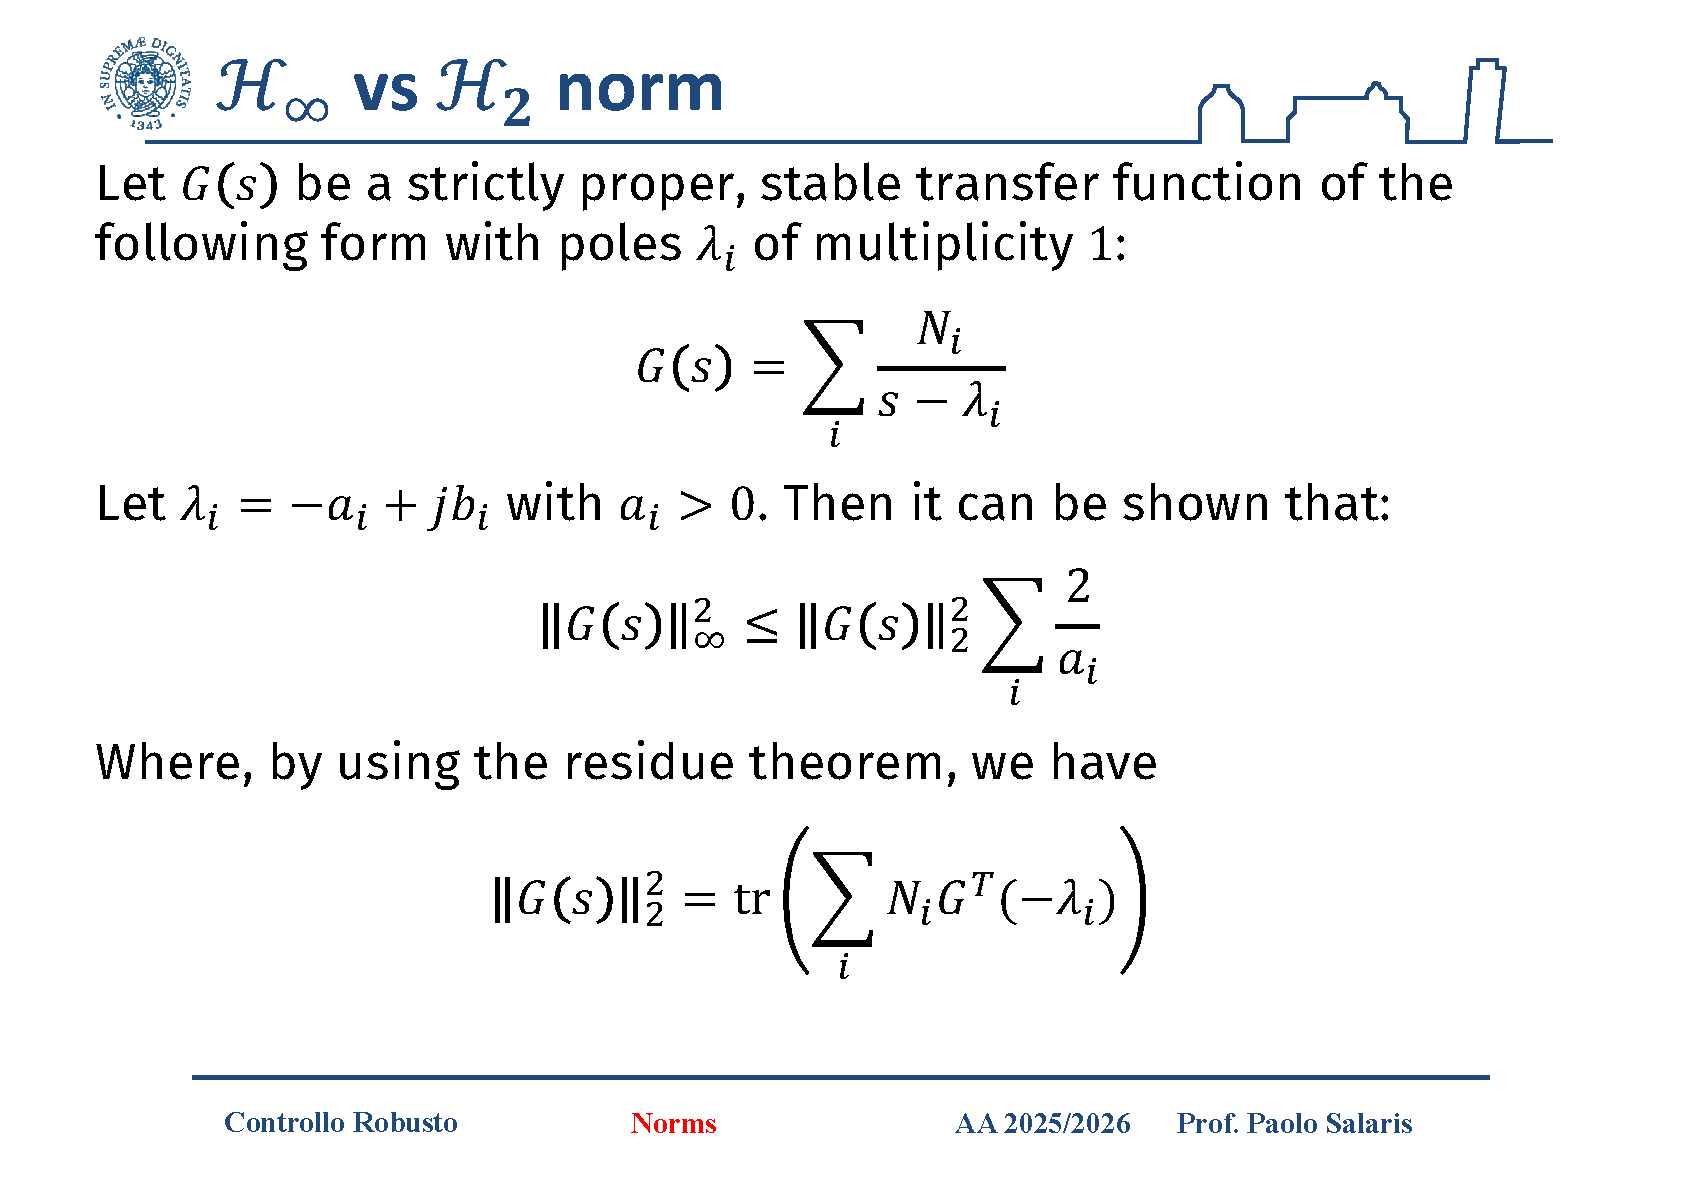
\includegraphics[width=0.82\textwidth]{images10/norms-new-60-76-013.png}
    \caption{In casi particolari si possono ottenere bound tra norma $H_\infty$ e norma $H_2$, ma il bound dipende dalla posizione dei poli.}
\end{figure}

\subsection{Perch\`e la norma \texorpdfstring{$H_\infty$}{H-infinito} \`e cos\`i usata}

La norma $H_\infty$ \`e molto popolare nel controllo robusto perch\'e si presta naturalmente alla modellazione dell'incertezza non strutturata. La propriet\`a chiave \`e la submoltiplicativit\`a:
$$
\|G_1(s)G_2(s)\|_{H_\infty}
\le
\|G_1(s)\|_{H_\infty}\,\|G_2(s)\|_{H_\infty}.
$$
Questa disuguaglianza \`e esattamente ci\`o che serve nei ragionamenti di piccolo guadagno: se un'incertezza e un canale chiuso sono collegati in cascata, il guadagno del prodotto \`e controllabile tramite il prodotto dei guadagni.

La norma $H_2$, invece, non \`e una norma indotta e non soddisfa in generale una propriet\`a moltiplicativa:
$$
\|G_1(s)G_2(s)\|_{H_2}
\nleq
\|G_1(s)\|_{H_2}\,\|G_2(s)\|_{H_2}.
$$
Per vedere il problema, prendiamo ancora
$$
G(s)=\frac{1}{s+a},
\qquad
\|G\|_{H_2}=\sqrt{\frac{1}{2a}}.
$$
Allora
$$
G(s)^2=\frac{1}{(s+a)^2},
\qquad
\mathcal{L}^{-1}\{G(s)^2\}=t e^{-at}.
$$
Quindi
$$
\|G(s)^2\|_{H_2}
=
\left(\int_0^\infty t^2e^{-2at}\,dt\right)^{1/2}
=
\frac{1}{2a^{3/2}}
=
\frac{1}{\sqrt{a}}\|G\|_{H_2}^2.
$$
Se $a<1$, allora
$$
\|G(s)^2\|_{H_2}>\|G(s)\|_{H_2}^2.
$$
Per la norma $H_\infty$, invece,
$$
\|G(s)^2\|_{H_\infty}
=
\frac{1}{a^2}
=
\|G(s)\|_{H_\infty}^2.
$$

\begin{figure}[H]
    \centering
    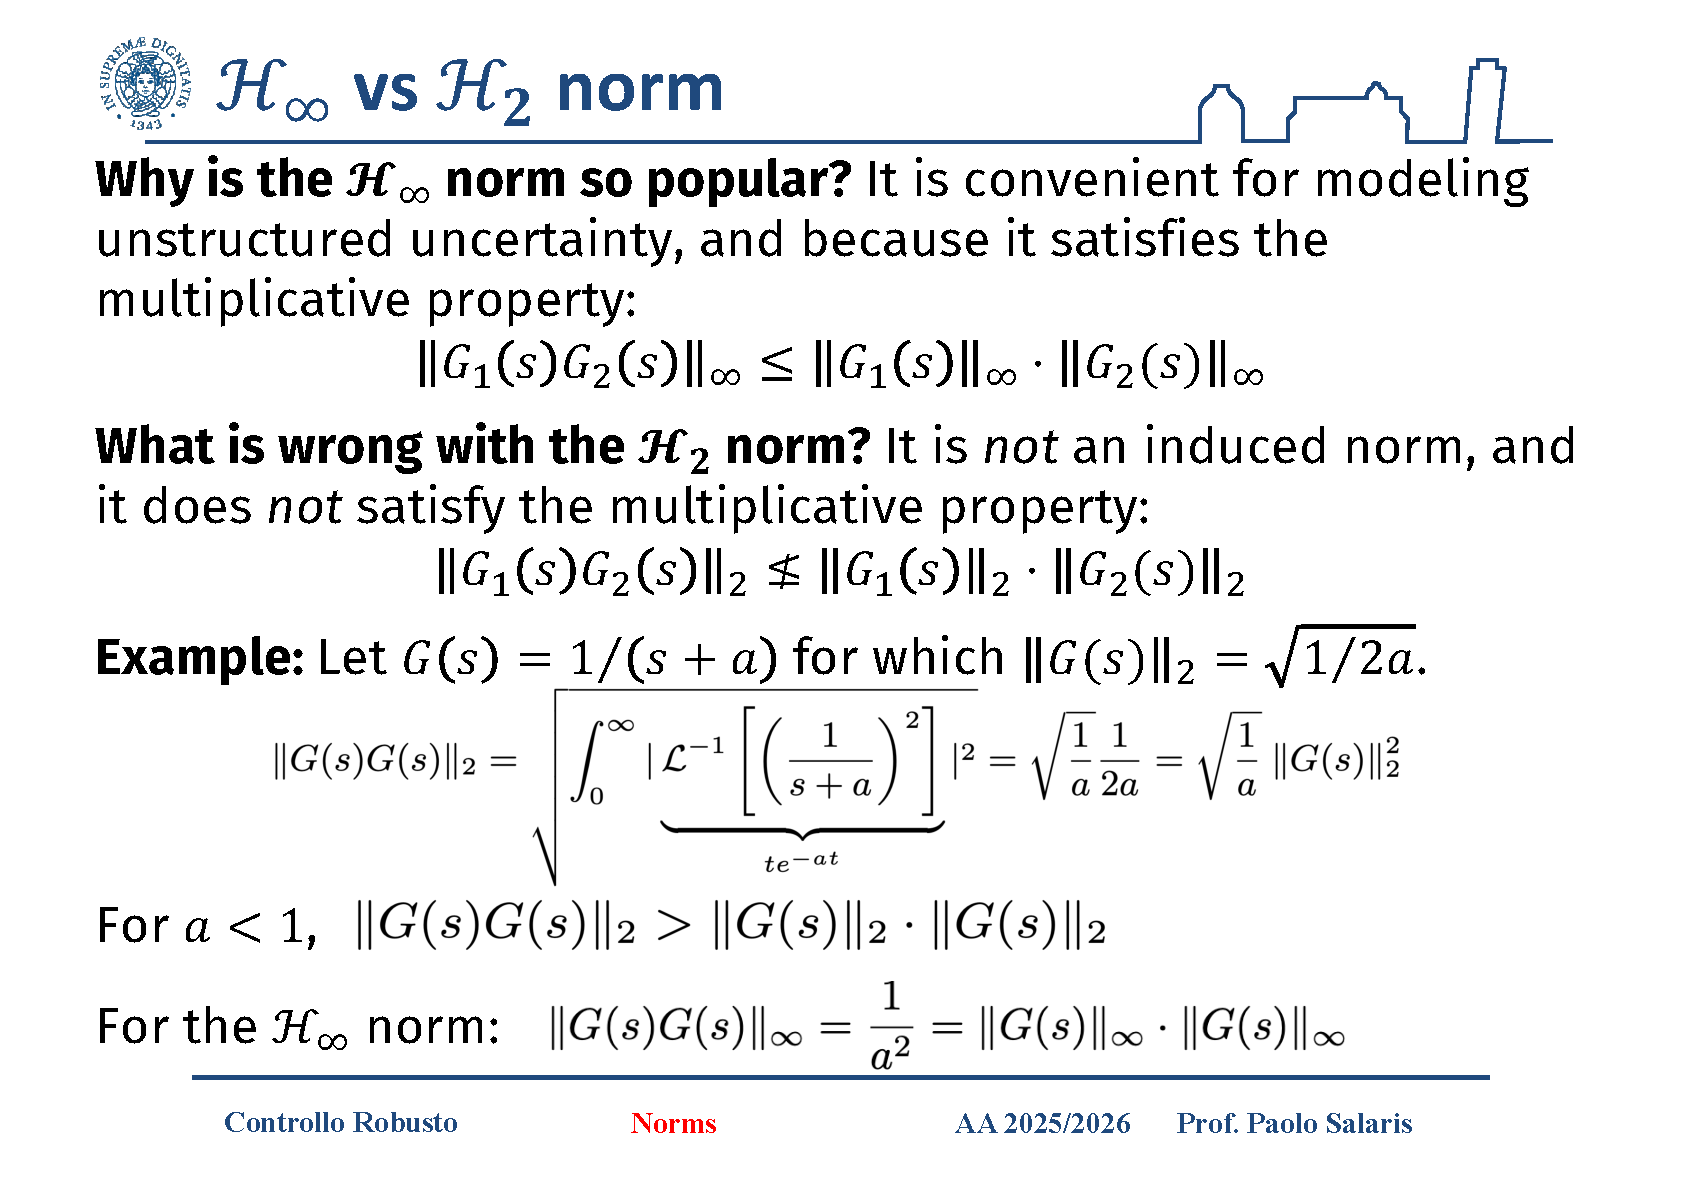
\includegraphics[width=0.82\textwidth]{images10/norms-new-60-76-014.png}
    \caption{La norma $H_\infty$ \`e submoltiplicativa, mentre la norma $H_2$ non lo \`e in generale. Questo spiega il ruolo centrale di $H_\infty$ nella robustezza.}
\end{figure}

\subsection{Norma di Hankel}

L'ultima parte della lezione introduce la norma di Hankel. Consideriamo un sistema stabile $G(s)$. Qui la domanda non \`e pi\`u ``quanto amplifico un ingresso sinusoidale?'' e nemmeno ``quanta energia ha la risposta impulsiva?''. La domanda \`e: quanta energia pu\`o essere immagazzinata nello stato dal passato e poi rilasciata nell'uscita futura?

Per questo la norma di Hankel misura il massimo rapporto tra:
\begin{itemize}
    \item l'energia dell'uscita futura $z(t)$ per $t>0$;
    \item l'energia dell'ingresso passato $w(t)$ applicato per $t<0$.
\end{itemize}
Formalmente,
$$
\|G\|_H
=
\max_{w\neq0}
\frac{
\left(
\int_0^\infty \|z(t)\|_2^2\,dt
\right)^{1/2}
}{
\left(
\int_{-\infty}^0 \|w(t)\|_2^2\,dt
\right)^{1/2}
}.
$$
L'interpretazione della slide \`e quella dell'altalena: si usa energia prima di $t=0$ per caricare lo stato del sistema, poi si guarda quanta uscita libera si ottiene dopo $t=0$. La norma di Hankel misura quindi il miglior compromesso possibile tra controllabilit\`a dal passato e osservabilit\`a nel futuro.

\begin{figure}[H]
    \centering
    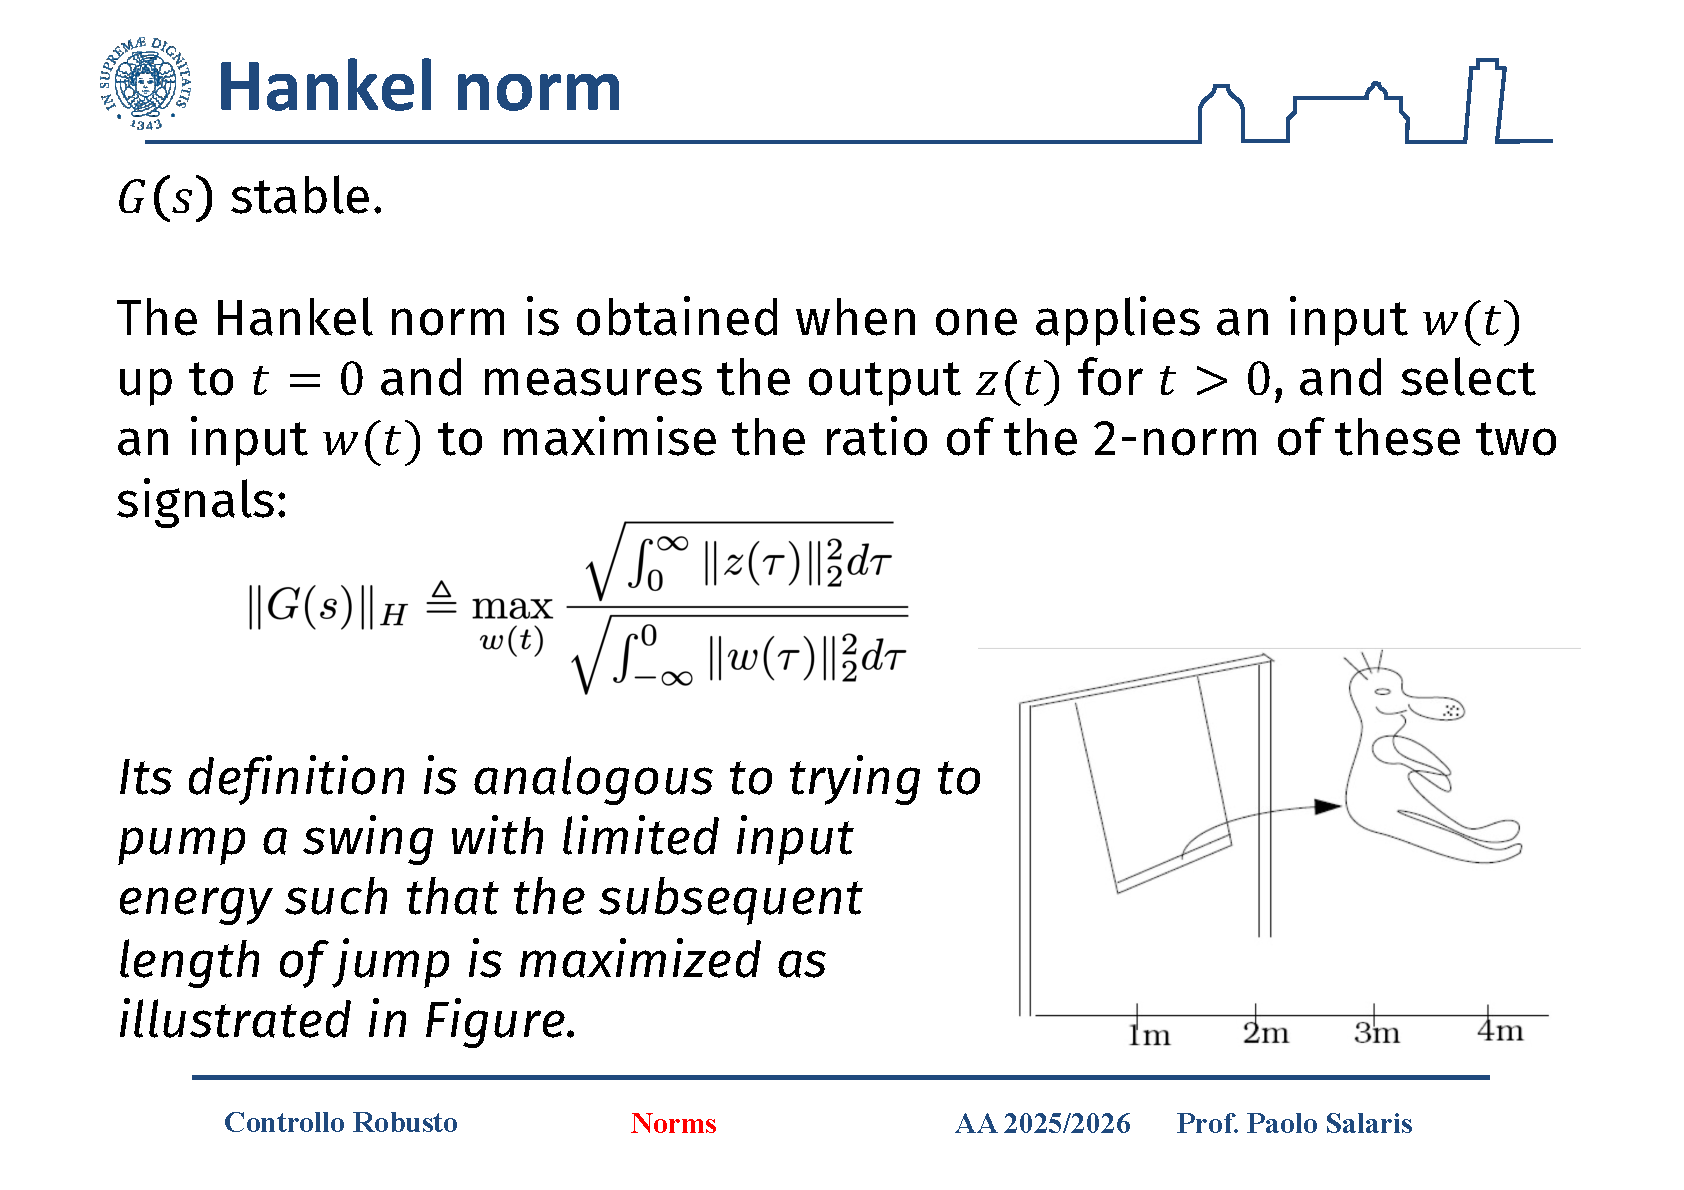
\includegraphics[width=0.82\textwidth]{images10/norms-new-60-76-015.png}
    \caption{Definizione energetica della norma di Hankel: ingresso nel passato, uscita nel futuro.}
\end{figure}

La slide successiva d\`a la formula computazionale. Per una realizzazione stabile e minimale, siano $P$ e $Q$ rispettivamente il gramiano di controllabilit\`a e il gramiano di osservabilit\`a, cio\`e le soluzioni di
$$
AP+PA^T+BB^T=0,
\qquad
A^TQ+QA+C^TC=0.
$$
Allora
$$
\|G(s)\|_H
=
\sqrt{\rho(PQ)},
$$
dove $\rho(\cdot)$ \`e il raggio spettrale, cio\`e il massimo valore assoluto degli autovalori. Anche se $PQ$ non \`e in generale simmetrica, i suoi autovalori rilevanti coincidono con quelli della matrice simmetrica simile $P^{1/2}QP^{1/2}$ quando $P$ \`e definita positiva; per questo le quantit\`a sotto radice sono non negative nel caso minimale stabile.

I numeri
$$
\sigma_i=\sqrt{\lambda_i(PQ)}
$$
sono detti \emph{valori singolari di Hankel}. Ordinandoli in modo decrescente,
$$
\sigma_1\ge\sigma_2\ge\cdots\ge\sigma_n,
$$
si ha
$$
\|G\|_H=\sigma_1.
$$
Le slide riportano anche il bound classico
$$
\|G\|_H=\sigma_1
\le
\|G\|_{H_\infty}
\le
2\sum_{i=1}^n\sigma_i.
$$
Questo legame spiega perch\'e la norma di Hankel sia importante nella riduzione di modello: i valori singolari di Hankel misurano quanto ciascuna direzione di stato sia insieme controllabile e osservabile.

Una nota terminologica evita un possibile equivoco: il nome ``Hankel'' deriva dall'operatore che mappa ingressi passati in uscite future, la cui matrice ha struttura di Hankel. Nelle formule di stato usate qui, questa informazione viene condensata nei gramiani tramite il prodotto $PQ$.

\begin{figure}[H]
    \centering
    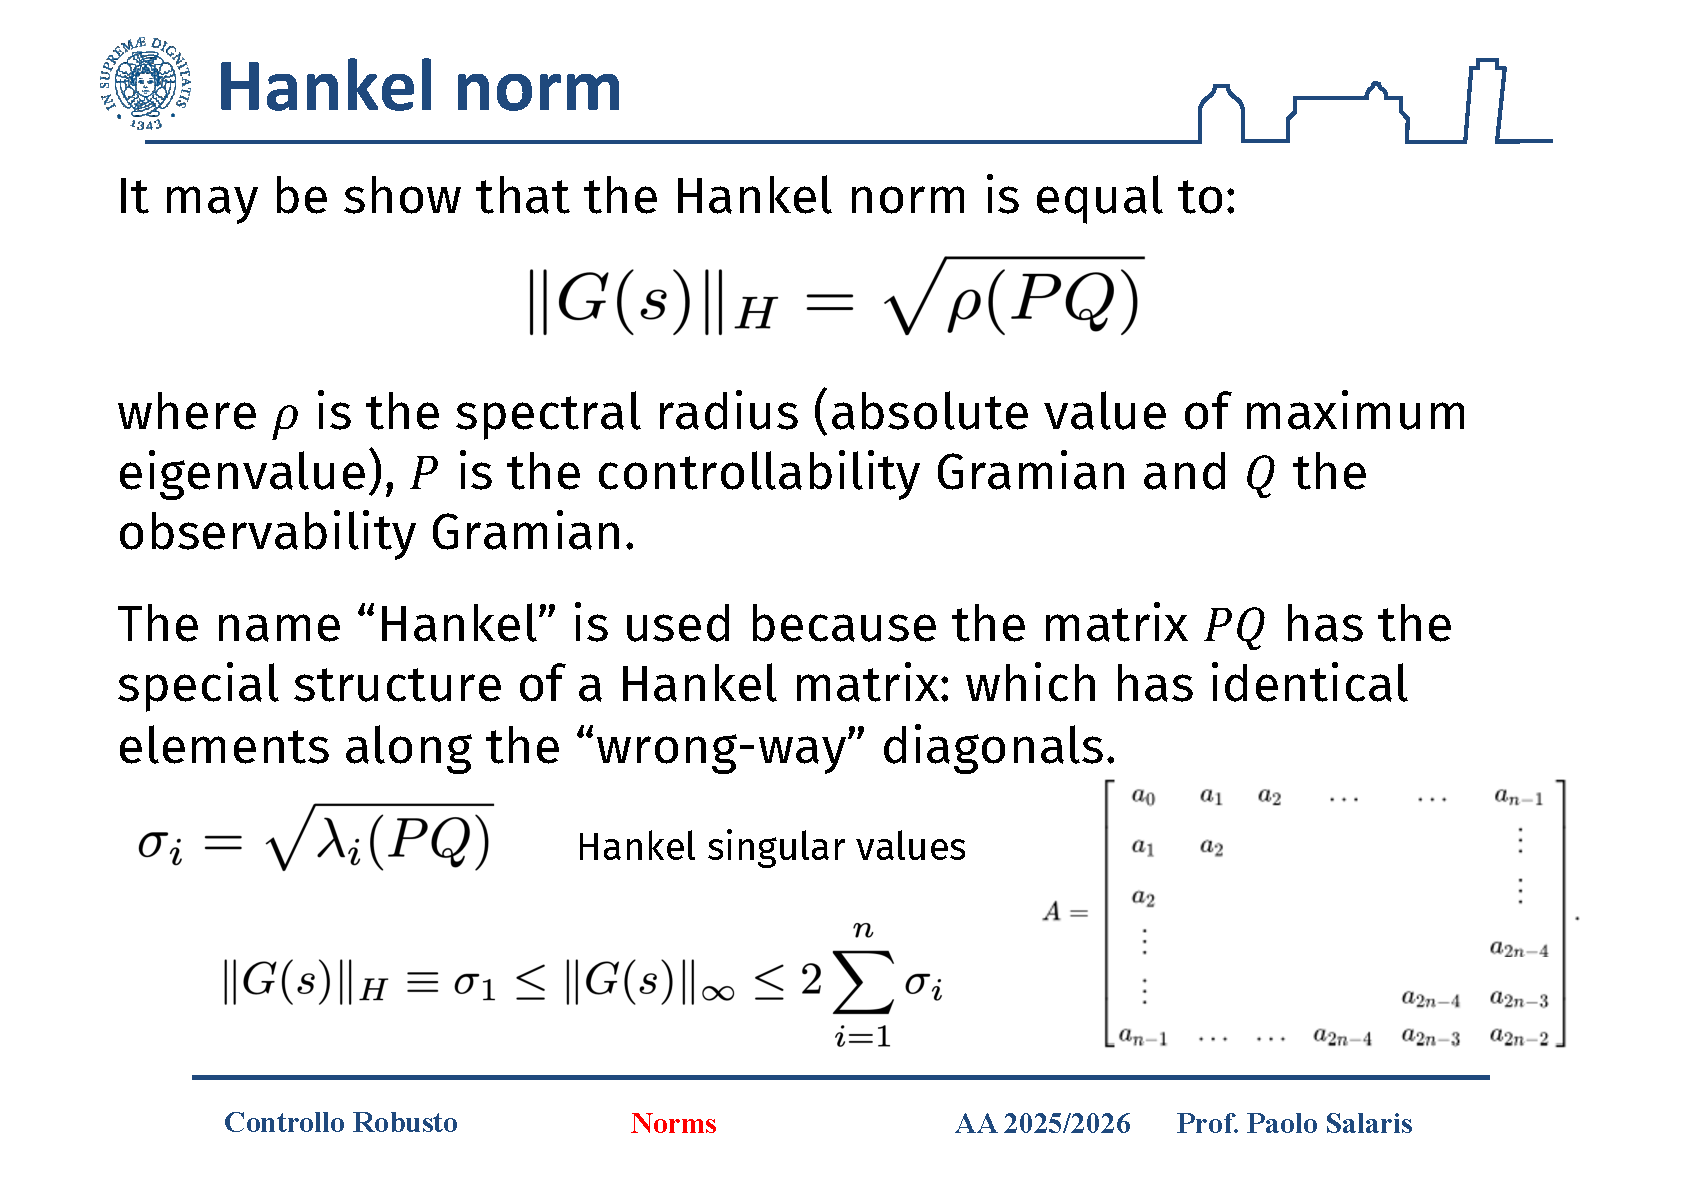
\includegraphics[width=0.82\textwidth]{images10/norms-new-60-76-016.png}
    \caption{La norma di Hankel si calcola da $PQ$ e coincide con il maggiore valore singolare di Hankel.}
\end{figure}

\subsection{Esempio finale: tutte le norme per \texorpdfstring{$G(s)=1/(s+a)$}{G(s)=1/(s+a)}}

La slide finale raccoglie i risultati per
$$
G(s)=\frac{1}{s+a},
\qquad
a>0.
$$
Una realizzazione di stato \`e
$$
A=-a,\qquad B=1,\qquad C=1,\qquad D=0.
$$
Il gramiano di controllabilit\`a si ottiene da
$$
AP+PA^T=-BB^T,
$$
cio\`e
$$
-aP-aP=-1,
\qquad
P=\frac{1}{2a}.
$$
Analogamente,
$$
Q=\frac{1}{2a}.
$$

La norma $H_2$ \`e
$$
\|G(s)\|_{H_2}
=
\sqrt{\operatorname{tr}(B^TQB)}
=
\sqrt{\frac{1}{2a}}.
$$
Per la norma $H_\infty$, la Hamiltoniana del bounded real lemma \`e
$$
\mathcal{H}_\gamma=
\begin{bmatrix}
-a & \gamma^{-2}\\
-1 & a
\end{bmatrix},
$$
con autovalori
$$
\lambda(\mathcal{H}_\gamma)
=
\pm\sqrt{a^2-\gamma^{-2}}.
$$
Essa non ha autovalori immaginari per
$$
\gamma>\frac{1}{a},
$$
quindi
$$
\|G(s)\|_{H_\infty}=\frac{1}{a}.
$$
Infine
$$
PQ=\frac{1}{4a^2},
$$
e la norma di Hankel vale
$$
\|G(s)\|_H
=
\sqrt{\rho(PQ)}
=
\frac{1}{2a}.
$$

\begin{figure}[H]
    \centering
    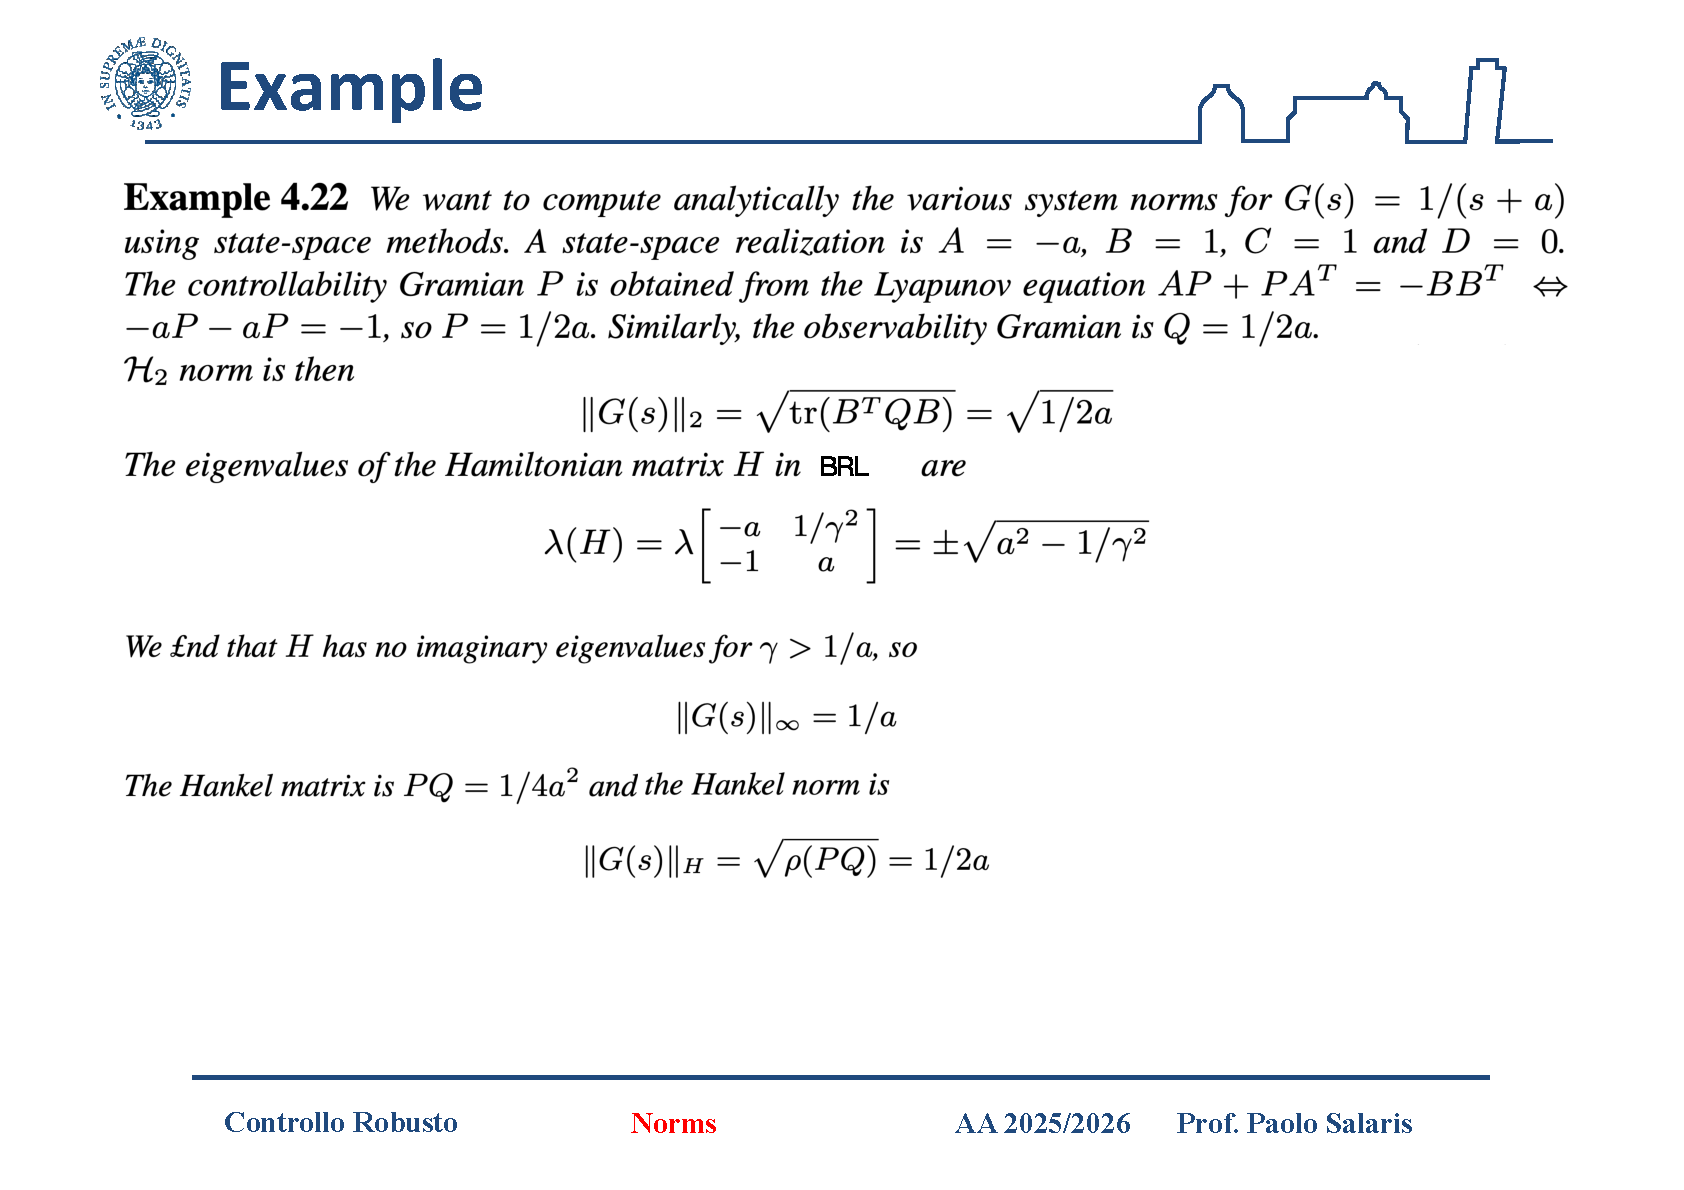
\includegraphics[width=0.82\textwidth]{images10/norms-new-60-76-017.png}
    \caption{Esempio riassuntivo: per $G(s)=1/(s+a)$ si calcolano esplicitamente norma $H_2$, norma $H_\infty$ e norma di Hankel.}
\end{figure}

\subsection{Sintesi conclusiva della lezione}

La Lezione 10 chiude il blocco sulle norme trasformando i risultati teorici in procedure operative. Il bounded real lemma diventa un algoritmo: si fissa una soglia $\gamma$, si testa la Hamiltoniana, e si restringe l'intervallo per bisezione fino a localizzare $\|G\|_{H_\infty}$. Negli esempi piccoli, la stessa soglia pu\`o essere trovata analiticamente con Routh--Hurwitz applicato al polinomio della Hamiltoniana.

Il confronto tra $H_\infty$ e $H_2$ chiarisce perch\'e nel controllo robusto la norma $H_\infty$ sia cos\`i centrale. $H_\infty$ controlla il caso peggiore ed \`e submoltiplicativa, quindi si combina bene con il piccolo guadagno e con l'incertezza non strutturata. $H_2$ misura invece un'energia distribuita, utilissima per rumore e risposta impulsiva, ma non sostituisce una garanzia di robustezza in cascata.

La norma di Hankel aggiunge una terza prospettiva: non guarda soltanto il guadagno frequenziale o l'energia totale, ma la capacit\`a del sistema di immagazzinare energia nello stato e restituirla in uscita. Per questo collega naturalmente controllabilit\`a, osservabilit\`a e riduzione di modello.

\clearpage
\phantomsection
\section*{Appendice}
\addcontentsline{toc}{section}{Appendice}

\subsection*{Riferimento al materiale originale}
\phantomsection
\addcontentsline{toc}{subsection}{Riferimento al materiale originale}

Questa parte del documento \`e una traduzione e rielaborazione estesa delle slide 60--76 del PDF aggiornato ``Norms for signals and systems'', caricato dall'utente come materiale di partenza. La riscrittura mantiene l'ordine delle slide: bisezione Hamiltoniana, Routh--Hurwitz, esempi, confronto $H_\infty/H_2$, submoltiplicativit\`a e norma di Hankel.

\begin{coverpage}
\centering
{\Huge\bfseries Controllo Robusto\par}
\vspace{0.4em}
{\LARGE Traduzione in italiano e approfondimento\par}
\vspace{0.5em}
{\Large Formulazione del problema di controllo robusto\par}
\vfill

\includegraphics[width=0.78\textwidth]{images11/formulation-01-21-001.png}
\vfill
\begin{focusbox}
\textbf{Obiettivo del documento.} Questa parte degli appunti apre il capitolo sulla formulazione dei problemi di controllo. L'idea centrale \`e passare da un singolo modello nominale a una famiglia di modelli possibili, descritta tramite incertezza parametrica, dinamica, additiva, moltiplicativa e inversa moltiplicativa. La lezione traduce le slide 1--21 e aggiunge i passaggi intermedi necessari per leggere correttamente le formule.
\end{focusbox}
\vfill
{\large Basato sulle slide del corso AA 2025/2026\par}
\end{coverpage}

\section{Lezione 11}

\subsection{Visione d'insieme della lezione}

Con la Lezione 10 si \`e concluso il blocco sulle norme dei segnali e dei sistemi. Quelle norme non sono state introdotte per gusto estetico: servono per dare una misura precisa a frasi come ``il sistema amplifica poco'', ``la perturbazione \`e piccola'' oppure ``l'errore resta limitato''. La Lezione 11 inizia a usare davvero questa cassetta degli attrezzi per formulare il problema di controllo robusto.

La domanda di fondo cambia leggermente. Finora spesso abbiamo ragionato su un sistema nominale $G(s)$. Da qui in avanti, invece, il processo reale non sar\`a pi\`u rappresentato da una sola funzione di trasferimento, ma da una famiglia
$$
G_p(s)\in\Pi,
$$
dove $\Pi$ contiene tutti i modelli compatibili con quello che sappiamo, con quello che non sappiamo e con quello che scegliamo consapevolmente di trascurare.

\begin{keybox}
\textbf{Idea guida.} Il controllo robusto non parte dalla domanda ``il controllore funziona su $G$?''. Parte dalla domanda pi\`u severa ``il controllore funziona su tutti i $G_p$ appartenenti alla famiglia di incertezza $\Pi$?''. Per rispondere bisogna specificare bene modello nominale, incertezza, ingressi e obiettivi di prestazione.
\end{keybox}

\subsection{I quattro ingredienti di un problema di controllo}

Una procedura di progetto produce un controllore credibile solo se vengono specificati quattro elementi. Se uno di questi manca, il problema resta ambiguo: si pu\`o anche ottenere un controllore numericamente elegante, ma non c'\`e nessuna garanzia che abbia senso sul sistema fisico.

Il primo elemento \`e il \textbf{modello del processo}. Si sceglie un modello nominale, idealmente perfetto ma in pratica sempre approssimato. Questo modello \`e il centro attorno al quale si costruisce il progetto.

Il secondo elemento \`e il \textbf{limite sull'incertezza di modello}. Bisogna dire quanto il processo reale pu\`o discostarsi dal nominale. L'incertezza pu\`o essere parametrica, quando si conosce la struttura del modello ma non esattamente il valore dei parametri, oppure dinamica, quando alcune dinamiche sono state trascurate o non sono note.

Il terzo elemento \`e il \textbf{tipo di ingressi}. Un problema di inseguimento di riferimento non \`e uguale a un problema di reiezione dei disturbi. Anche la posizione in cui entrano disturbi e rumori cambia le funzioni di trasferimento che devono essere rese piccole.

Il quarto elemento \`e l'\textbf{obiettivo di prestazione}. Bisogna specificare che cosa significa ``funzionare bene'': piccolo errore a bassa frequenza, attenuazione del rumore, limiti sul comando, rapidit\`a di risposta, robustezza ai parametri oppure una combinazione pesata di questi requisiti.

\begin{figure}[H]
    \centering
    \begin{subfigure}{0.32\textwidth}
        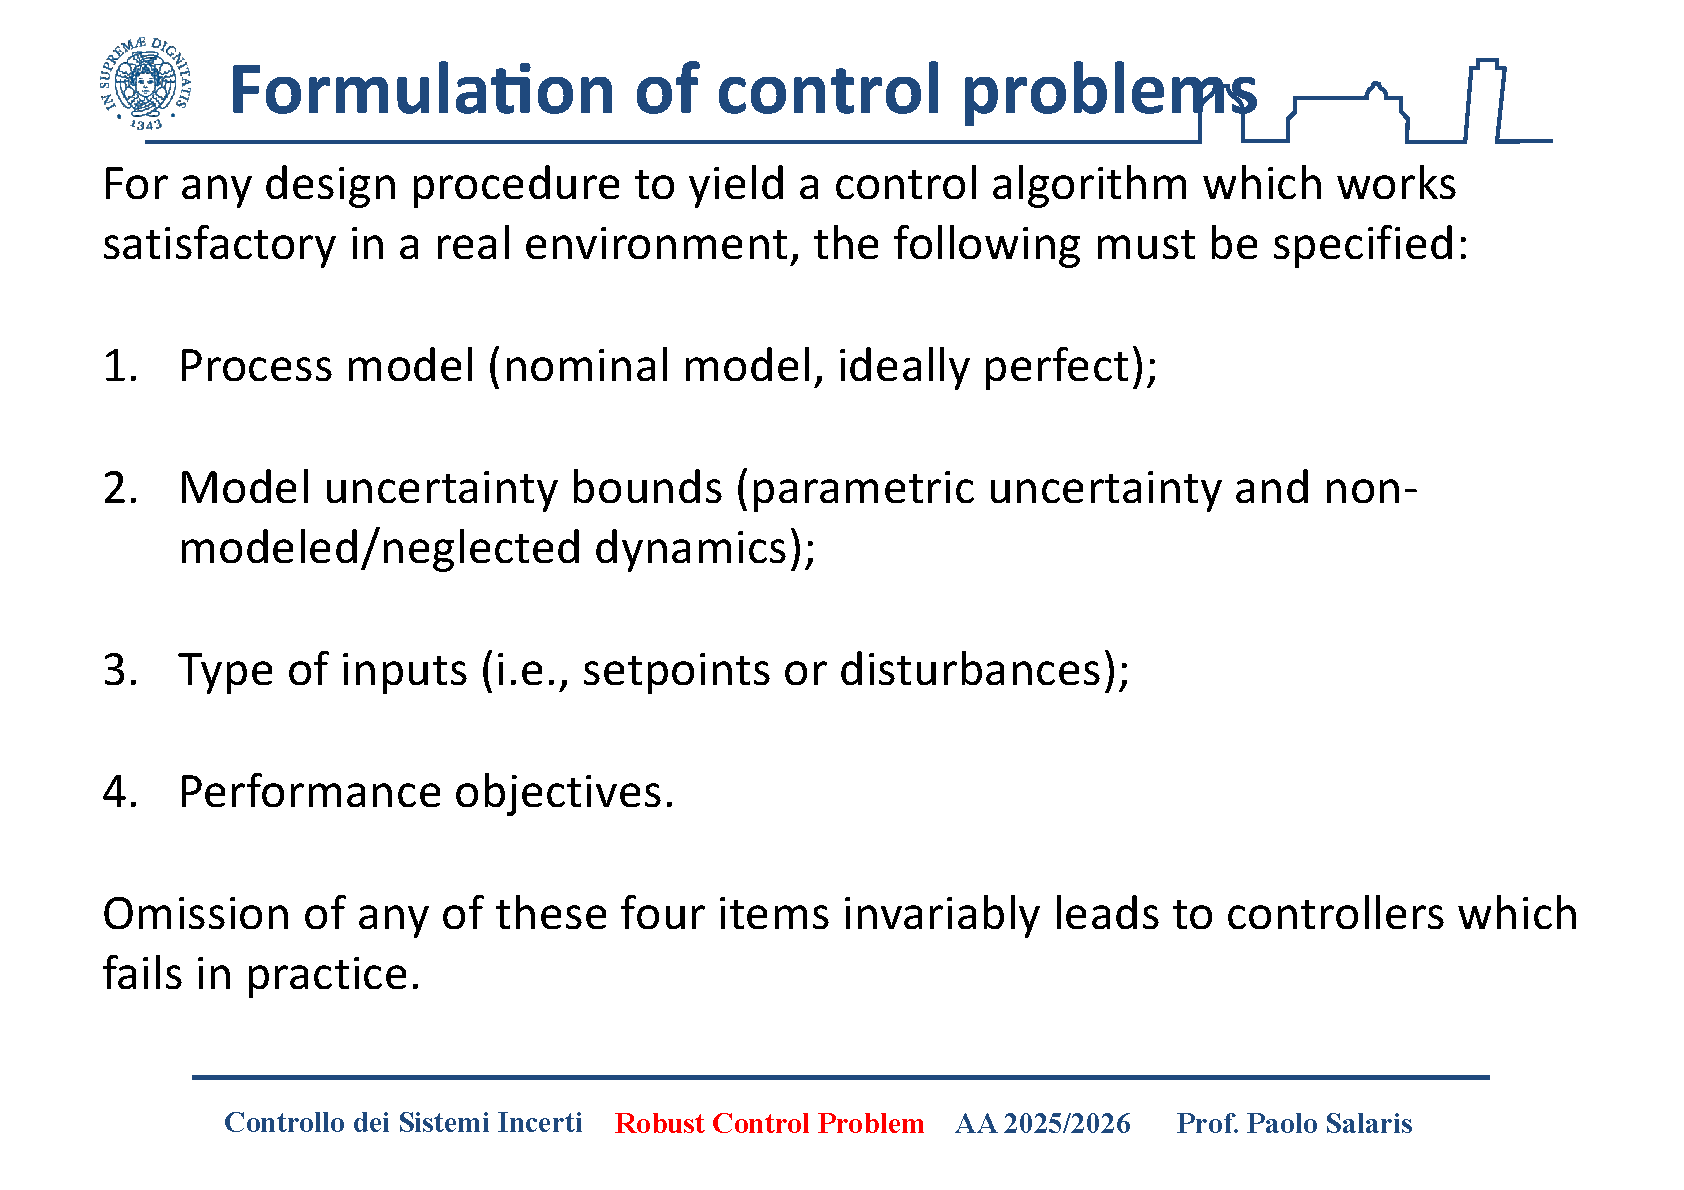
\includegraphics[width=\linewidth]{images11/formulation-01-21-002.png}
        \caption{Ingredienti del problema di progetto.}
    \end{subfigure}
    \hfill
    \begin{subfigure}{0.32\textwidth}
        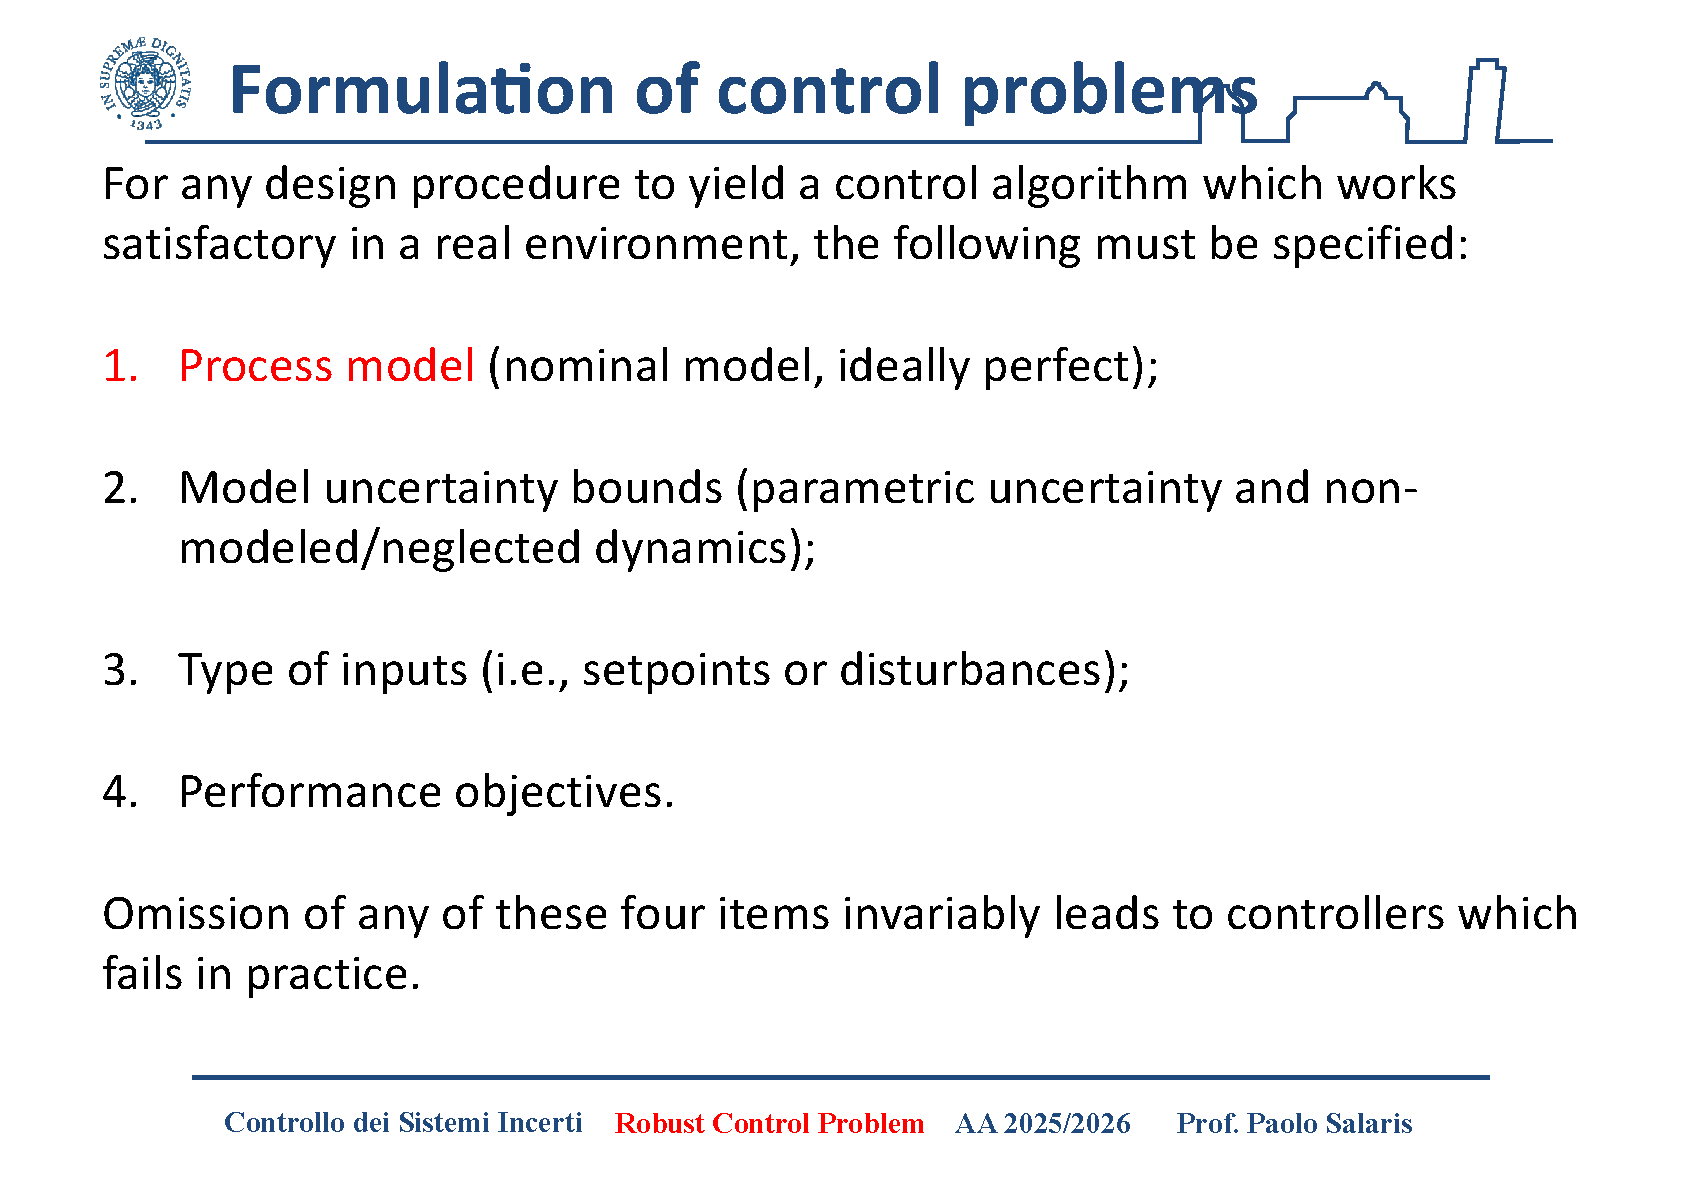
\includegraphics[width=\linewidth]{images11/formulation-01-21-003.png}
        \caption{Richiamo della stessa struttura logica.}
    \end{subfigure}
    \hfill
    \begin{subfigure}{0.32\textwidth}
        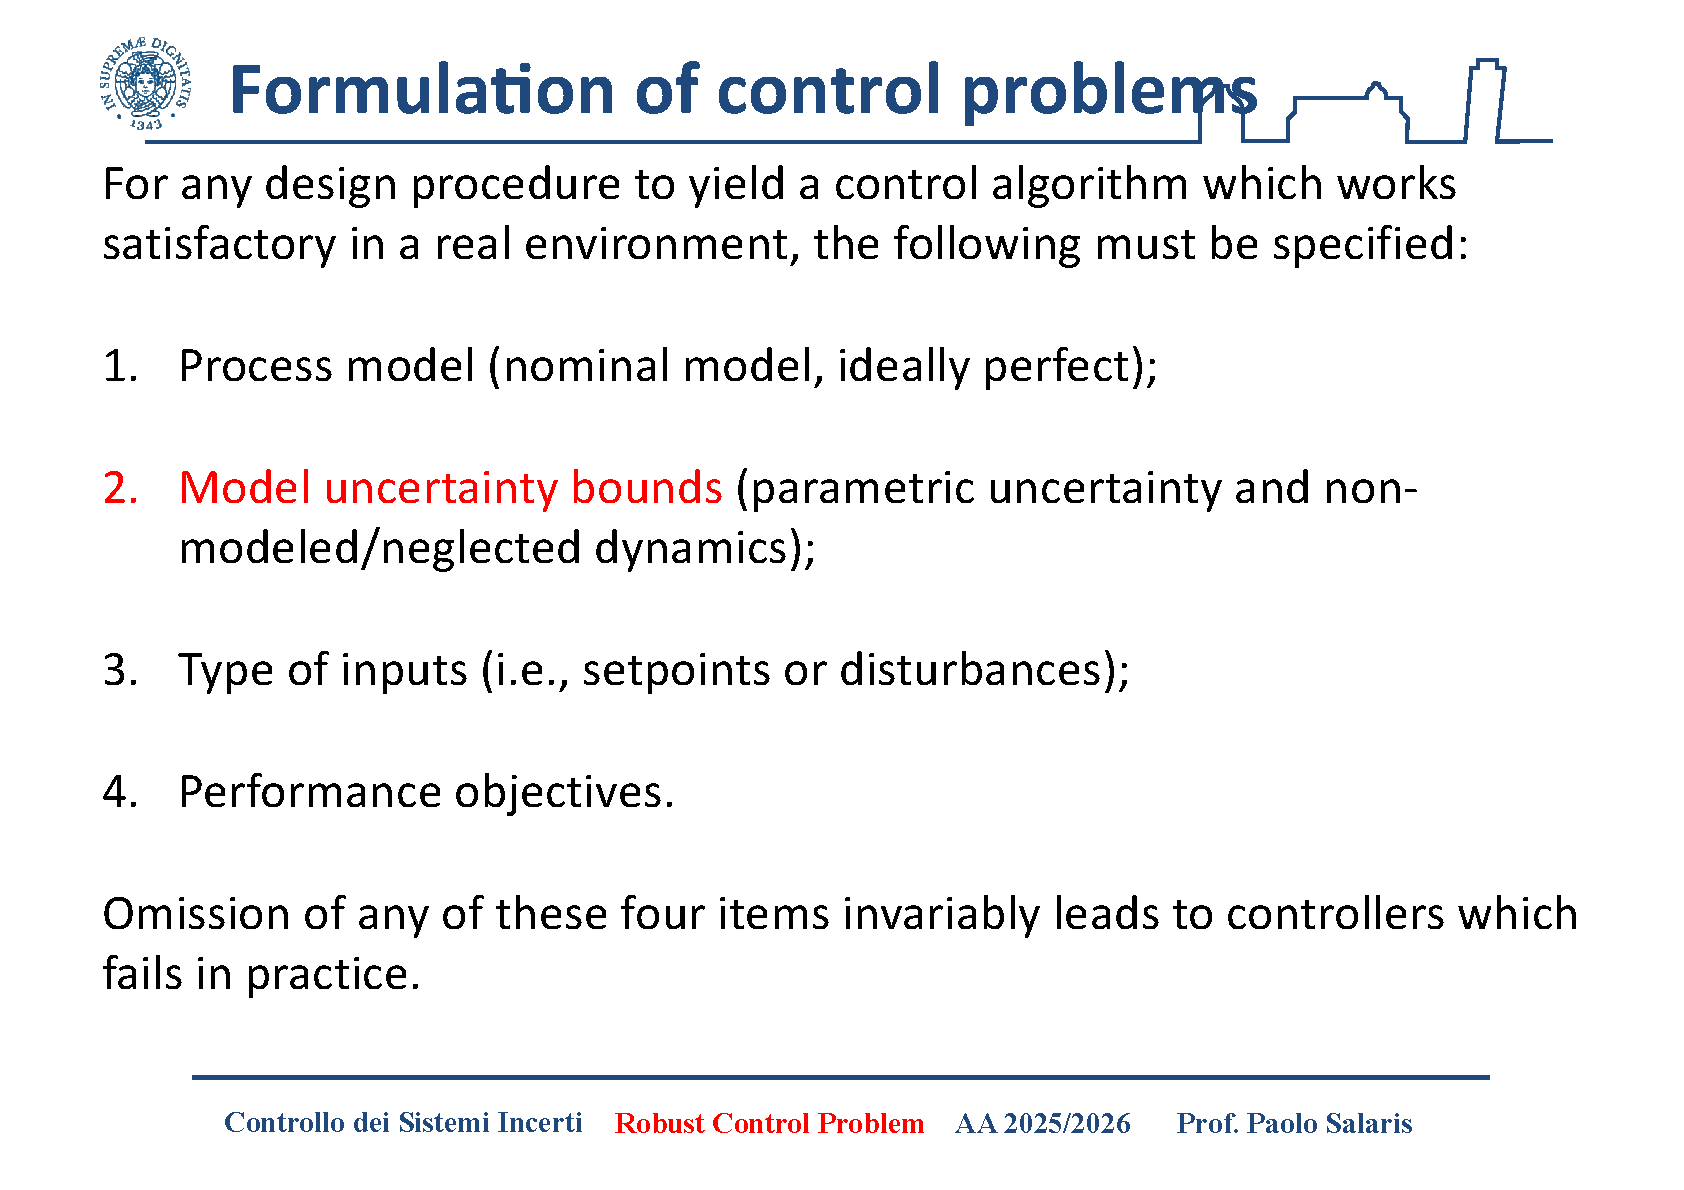
\includegraphics[width=\linewidth]{images11/formulation-01-21-005.png}
        \caption{Transizione verso l'incertezza di modello.}
    \end{subfigure}
    \caption{Le slide insistono sullo stesso punto: un problema robusto deve dichiarare modello, incertezza, ingressi e specifiche.}
\end{figure}

\subsection{Modello del processo}

Il modello di partenza \`e una funzione di trasferimento lineare nel caso SISO, oppure una matrice di trasferimento nel caso MIMO. Per un sistema SISO con ritardo si scrive
$$
G(s)=\frac{n(s)}{d(s)}e^{-\tau s}.
$$
Qui $n(s)$ e $d(s)$ sono polinomi, mentre $e^{-\tau s}$ rappresenta un ritardo puro di durata $\tau$.

Nel caso MIMO si ha una matrice
$$
G(s)=
\begin{bmatrix}
G_{11}(s) & \cdots & G_{1m}(s)\\
\vdots & \ddots & \vdots\\
G_{n1}(s) & \cdots & G_{nm}(s)
\end{bmatrix},
$$
dove ogni canale ingresso--uscita pu\`o avere un proprio ritardo:
$$
G_{ij}(s)=\frac{n_{ij}(s)}{d_{ij}(s)}e^{-\tau_{ij}s}.
$$

Il punto delicato \`e il ritardo. A bassa frequenza un ritardo puro pu\`o essere approssimato molto bene con un'approssimazione di Pad\'e. Per esempio, una forma del primo ordine \`e
$$
e^{-\tau s}\simeq \frac{1-\frac{\tau}{2}s}{1+\frac{\tau}{2}s}.
$$
Questa approssimazione per\`o non pu\`o essere perfetta su tutte le frequenze: un ritardo puro ha fase che decresce senza limite, mentre un modello razionale finito no. Per questo la differenza ad alta frequenza fra ritardo vero e approssimazione finito-dimensionale viene trattata come incertezza di modello.

\begin{focusbox}
\textbf{Nota di modellazione.} Il modello usato nel progetto deve essere causale, cio\`e proprio: non pu\`o richiedere informazioni future dell'ingresso. In termini di funzioni di trasferimento, il grado del numeratore non deve superare il grado del denominatore.
\end{focusbox}

\begin{figure}[H]
    \centering
    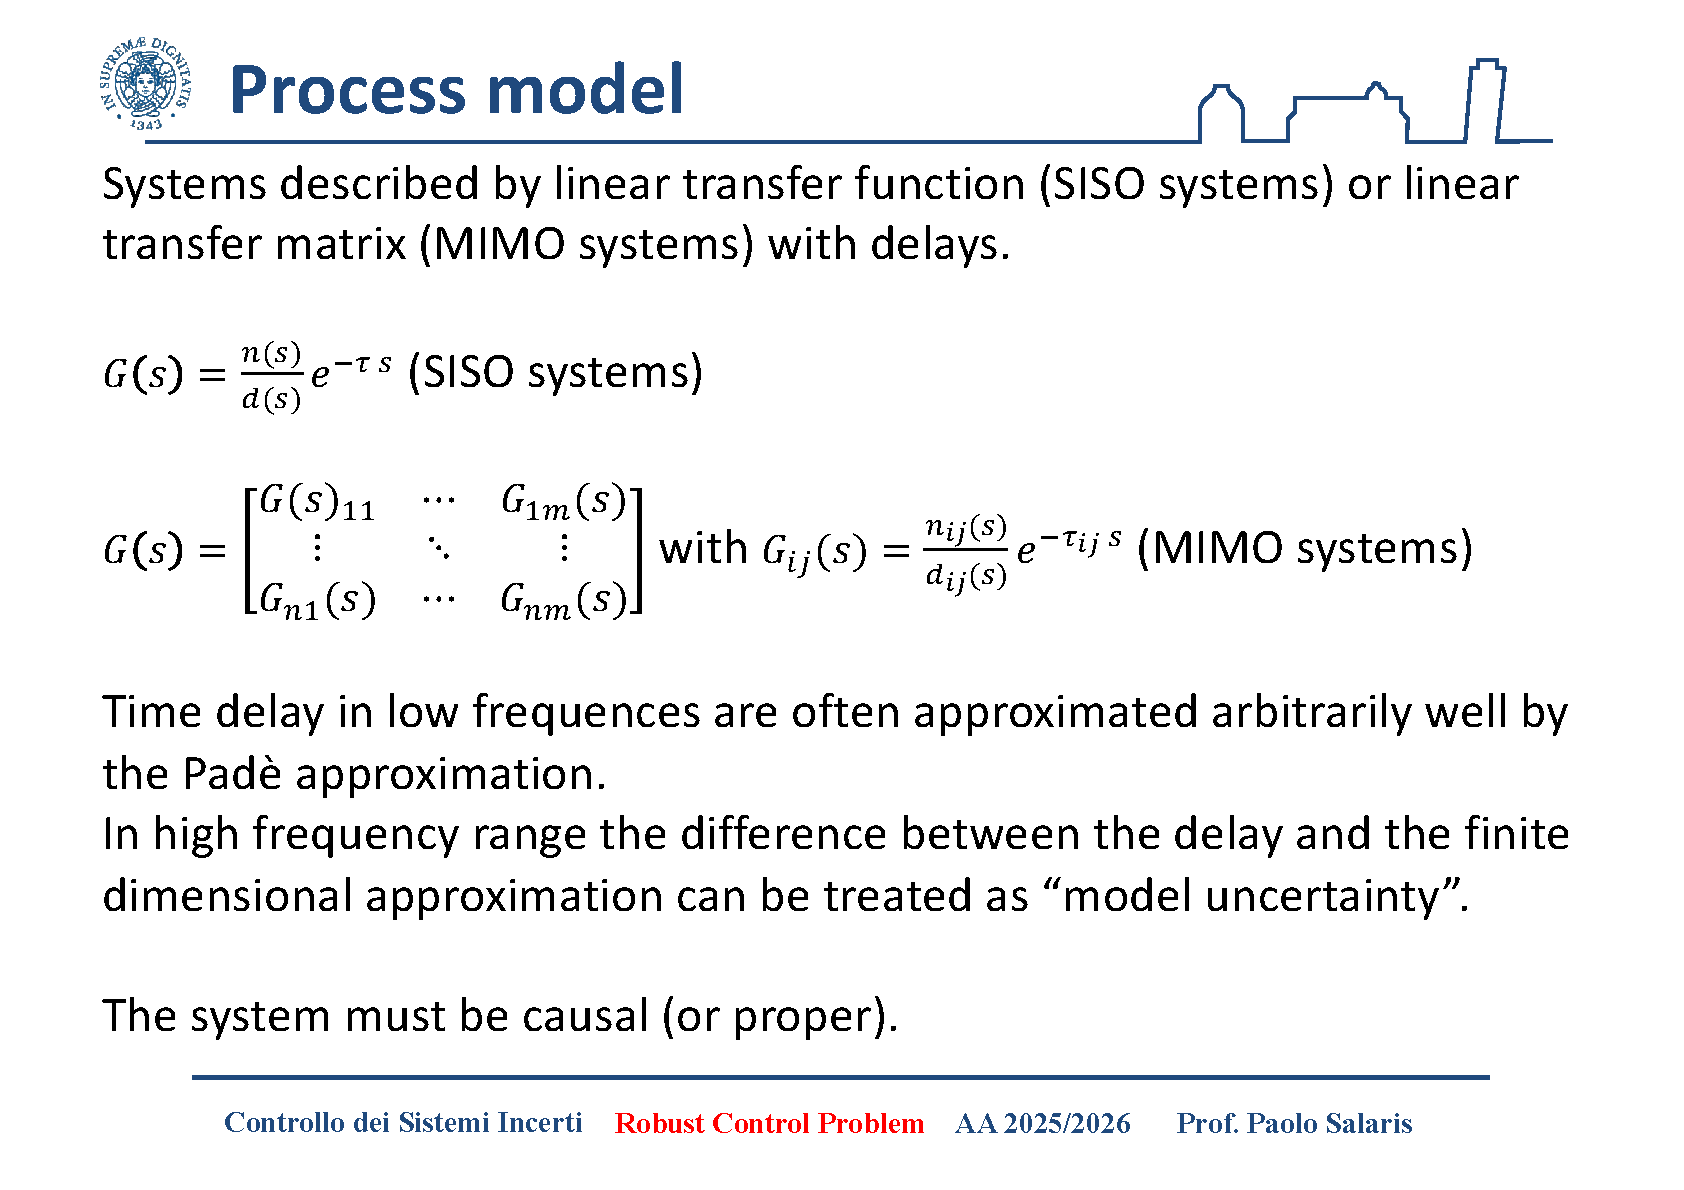
\includegraphics[width=0.82\textwidth]{images11/formulation-01-21-004.png}
    \caption{Modello del processo: funzioni di trasferimento SISO, matrici di trasferimento MIMO e ritardi.}
\end{figure}

\subsection{Incertezza di modello e obiettivi robusti}

Una volta scelto il modello nominale $G$, bisogna descrivere l'insieme dei possibili processi reali. Questo insieme viene indicato con $\Pi$ e contiene i modelli perturbati $G_p$:
$$
G_p\in\Pi.
$$

La slide propone una procedura in tre passi. Prima si determina l'\textbf{insieme di incertezza}: una descrizione matematica di ci\`o che sappiamo di non sapere. In pratica non serve soltanto dire ``il modello \`e incerto'', ma bisogna assegnare una forma all'incertezza e un limite quantitativo.

Poi si verifica la \textbf{stabilit\`a robusta}, indicata spesso con RS, da \emph{Robust Stability}. Essa richiede che il sistema in anello chiuso resti stabile per ogni processo appartenente alla famiglia:
$$
G_p\in\Pi.
$$
Non basta quindi che il controllore stabilizzi $G$: deve stabilizzare tutti i modelli ammissibili.

Infine si verifica la \textbf{prestazione robusta}, indicata con RP, da \emph{Robust Performance}. Questa richiede che, oltre alla stabilit\`a, le specifiche di prestazione siano soddisfatte per tutti i modelli della famiglia. La gerarchia concettuale \`e importante:
$$
\text{prestazione robusta} \quad\Longrightarrow\quad \text{stabilit\`a robusta}.
$$
Se il sistema non \`e robustamente stabile, non ha senso parlare di prestazioni robuste.

\begin{figure}[H]
    \centering
    \includegraphics[width=0.82\textwidth]{images11/formulation-01-21-006.png}
    \caption{Procedura generale: definire l'incertezza, verificare stabilit\`a robusta e poi prestazione robusta.}
\end{figure}

\subsection{Da dove nasce l'incertezza}

L'incertezza non \`e un dettaglio patologico: \`e la condizione normale di ogni modello fisico. Le slide elencano diverse origini.

Una prima sorgente sono i \textbf{parametri incerti}. Anche se la struttura del modello \`e corretta, masse, attriti, guadagni, costanti di tempo e coefficienti possono essere noti solo entro un intervallo.

Una seconda sorgente \`e la \textbf{variazione del punto operativo}. Un modello lineare descrive bene il sistema solo attorno a una certa condizione di funzionamento. Se il processo \`e non lineare, cambiando punto operativo cambiano anche i parametri equivalenti.

Una terza sorgente sono le \textbf{imperfezioni di misura}. Sensori con risoluzione finita, rumore, offset e dinamiche non modellate alterano la descrizione ingresso--uscita disponibile per il controllore.

La sorgente pi\`u importante nel controllo robusto \`e per\`o spesso la \textbf{dinamica trascurata}. A frequenze alte quasi nessun modello mantiene la struttura esatta del sistema reale. Questo non \`e necessariamente un errore: spesso si sceglie volontariamente un modello nominale di ordine basso, pi\`u semplice da usare nel progetto, e si rappresenta il resto come incertezza.

Anche il controllore realizzato pu\`o differire da quello progettato. Per esempio, un controllore di ordine alto pu\`o essere ridotto prima dell'implementazione, oppure pu\`o subire approssimazioni numeriche. Anche queste differenze possono essere inglobate nella descrizione di incertezza.

\begin{figure}[H]
    \centering
    \includegraphics[width=0.82\textwidth]{images11/formulation-01-21-007.png}
    \caption{Origini dell'incertezza: parametri, nonlinearit\`a, sensori, dinamiche trascurate e implementazione del controllore.}
\end{figure}

\subsection{Incertezza parametrica e incertezza dinamica}

Le slide distinguono due classi principali. La prima \`e l'\textbf{incertezza parametrica}, detta anche reale o strutturata. In questo caso la struttura del modello, incluso l'ordine, \`e nota; non sono noti esattamente alcuni parametri. Se un parametro incerto $\alpha_p$ appartiene all'intervallo
$$
\alpha_{\min}\le \alpha_p\le \alpha_{\max},
$$
si introduce il valore medio
$$
\bar{\alpha}=\frac{\alpha_{\max}+\alpha_{\min}}{2}
$$
e l'incertezza relativa
$$
r_\alpha=
\frac{\alpha_{\max}-\alpha_{\min}}
{\alpha_{\max}+\alpha_{\min}}.
$$
Allora ogni valore ammissibile pu\`o essere scritto nella forma normalizzata
$$
\alpha_p=\bar{\alpha}(1+r_\alpha\Delta),
\qquad
|\Delta|\le 1.
$$

Questa scrittura \`e molto comoda perch\'e separa tre informazioni: il valore nominale $\bar{\alpha}$, la dimensione relativa dell'incertezza $r_\alpha$ e la perturbazione normalizzata $\Delta$. Quando $|\Delta|\le1$, tutti i valori possibili del parametro sono coperti.

La seconda classe \`e l'\textbf{incertezza dinamica non modellata}. Qui non si tratta solo di un parametro sbagliato: mancano dinamiche intere, spesso ad alta frequenza. Questa incertezza \`e detta non strutturata perch\'e non sappiamo descriverla con pochi parametri reali. La si modella allora nel dominio della frequenza tramite una perturbazione complessa normalizzata:
$$
|\Delta(j\omega)|\le1
\qquad\forall\omega,
$$
oppure, in forma compatta,
$$
\|\Delta\|_\infty\le1.
$$

\begin{figure}[H]
    \centering
    \begin{subfigure}{0.48\textwidth}
        \includegraphics[width=\linewidth]{images11/formulation-01-21-008.png}
        \caption{Incertezza parametrica reale e strutturata.}
    \end{subfigure}
    \hfill
    \begin{subfigure}{0.48\textwidth}
        \includegraphics[width=\linewidth]{images11/formulation-01-21-009.png}
        \caption{Incertezza dinamica non modellata.}
    \end{subfigure}
    \caption{Due modi complementari di rappresentare ci\`o che non si conosce: parametri reali incerti oppure perturbazioni dinamiche complesse.}
\end{figure}

\subsection{Famiglie di piante e bande di Nyquist}

Quando il processo \`e incerto, a una certa frequenza $\omega$ il valore $G_p(j\omega)$ non \`e un singolo punto del piano complesso. \`E una regione di valori possibili. Al variare di $\omega$, queste regioni formano una specie di ``banda'' attorno al diagramma di Nyquist nominale.

Formalmente, per ogni frequenza si pu\`o pensare a un insieme
$$
\Pi(\omega)=\{G_p(j\omega):G_p\in\Pi\}.
$$
Il modello nominale $G(j\omega)$ \`e un punto della regione, spesso scelto come centro. Il processo reale, invece, pu\`o trovarsi in un qualunque punto ammesso dalla regione.

Questa immagine \`e molto utile concettualmente, ma non sempre \`e comoda per il progetto. Le regioni di Nyquist prodotte da parametri reali incerti possono avere forme geometriche complicate. Per costruire criteri robusti maneggevoli, si cerca spesso di racchiuderle con dischi o con descrizioni pesate pi\`u semplici.

\begin{figure}[H]
    \centering
    \begin{subfigure}{0.48\textwidth}
        \includegraphics[width=\linewidth]{images11/formulation-01-21-010.png}
        \caption{Una famiglia di modelli produce regioni frequenziali, non singoli punti.}
    \end{subfigure}
    \hfill
    \begin{subfigure}{0.48\textwidth}
        \includegraphics[width=\linewidth]{images11/formulation-01-21-011.png}
        \caption{Bande di Nyquist e regioni ammissibili nel piano complesso.}
    \end{subfigure}
    \caption{La descrizione robusta sostituisce il singolo diagramma di Nyquist con un insieme di possibili diagrammi.}
\end{figure}

\subsection{Dal reale al complesso: conservativit\`a e lumping}

Un passaggio molto frequente nel controllo robusto consiste nel sostituire una perturbazione reale
$$
|\Delta|\le1
$$
con una perturbazione complessa dipendente dalla frequenza
$$
|\Delta(j\omega)|\le1
\qquad\forall\omega.
$$
Questo passaggio \`e conservativo: una perturbazione complessa pu\`o assumere molti pi\`u valori di una perturbazione reale. In altre parole, si allarga l'insieme dei modelli possibili. Se il controllore funziona su questo insieme pi\`u grande, allora funziona certamente anche sull'insieme reale originale; per\`o si pu\`o perdere prestazione o rendere il problema pi\`u difficile.

Quando ci sono molte perturbazioni reali, il conservativismo pu\`o per\`o ridursi raggruppandole in una singola perturbazione complessa equivalente. Questo processo si chiama \textbf{lumping}. Una \emph{lumped uncertainty} combina una o pi\`u sorgenti di incertezza parametrica e/o dinamica non modellata dentro una sola perturbazione, scelta con una struttura adatta al problema.

\begin{figure}[H]
    \centering
    \includegraphics[width=0.82\textwidth]{images11/formulation-01-21-012.png}
    \caption{Rappresentare incertezze reali con perturbazioni complesse \`e conservativo, ma consente descrizioni robuste pi\`u semplici.}
\end{figure}

\subsection{Approssimazione a dischi delle regioni di incertezza}

La slide mostra un esempio con tre parametri incerti:
$$
G_p(s)=\frac{k}{\tau s+1}e^{-\theta s},
\qquad
2\le k,\theta,\tau\le3.
$$
Al variare di $k$, $\theta$ e $\tau$, il valore $G_p(j\omega)$ descrive una regione diversa per ogni frequenza. Queste regioni possono essere irregolari, soprattutto quando il ritardo modifica la fase.

Per ottenere una descrizione utilizzabile, si racchiude ciascuna regione in un disco. Si assume quindi che, per ogni $\omega$, i possibili valori di $G_p(j\omega)$ stiano entro un disco centrato in $G(j\omega)$ e di raggio $\bar{\ell}_a(\omega)$:
$$
\Pi=
\left\{
G_p:\ |G_p(j\omega)-G(j\omega)|\le \bar{\ell}_a(\omega)
\right\}.
$$
Il raggio $\bar{\ell}_a(\omega)$ misura l'errore assoluto massimo fra pianta reale e pianta nominale.

Di solito $\bar{\ell}_a(\omega)$ cresce con la frequenza. Questo \`e coerente con l'idea fisica: il modello nominale viene scelto per descrivere bene il comportamento a bassa frequenza, mentre ad alta frequenza si accetta una descrizione pi\`u incerta.

\begin{figure}[H]
    \centering
    \begin{subfigure}{0.48\textwidth}
        \includegraphics[width=\linewidth]{images11/formulation-01-21-013.png}
        \caption{Esempio con guadagno, costante di tempo e ritardo incerti.}
    \end{subfigure}
    \hfill
    \begin{subfigure}{0.48\textwidth}
        \includegraphics[width=\linewidth]{images11/formulation-01-21-014.png}
        \caption{Regioni approssimate da dischi centrati sul nominale.}
    \end{subfigure}
    \caption{Una regione parametrica complicata pu\`o essere racchiusa in dischi di incertezza frequenziale.}
\end{figure}

\subsection{Incertezza additiva}

La prima struttura standard \`e l'\textbf{incertezza additiva}. Si parte dalla descrizione a dischi:
$$
G_p(j\omega)=G(j\omega)+\ell_a(j\omega),
\qquad
|\ell_a(j\omega)|\le \bar{\ell}_a(\omega).
$$
L'errore $\ell_a$ \`e un errore assoluto: dice quanto il processo reale pu\`o spostarsi rispetto al nominale nel piano complesso.

Per renderlo compatibile con la teoria $H_\infty$, si fattorizza l'errore in un peso noto e una perturbazione normalizzata:
$$
\ell_a(j\omega)=w_A(j\omega)\Delta_A(j\omega),
\qquad
|\Delta_A(j\omega)|\le1.
$$
La famiglia additiva \`e quindi
$$
\Pi_A:
\quad
G_p(s)=G(s)+w_A(s)\Delta_A(s),
\qquad
\|\Delta_A\|_\infty\le1.
$$

Il peso $w_A(s)$ stabilisce la dimensione e la forma frequenziale dell'incertezza. Se l'errore di modello \`e piccolo a bassa frequenza e grande ad alta frequenza, allora $|w_A(j\omega)|$ sar\`a piccolo a bassa frequenza e pi\`u grande ad alta frequenza.

La perturbazione $\Delta_A$ contiene invece tutto ci\`o che non vogliamo modellare nel dettaglio, ma con la normalizzazione
$$
\|\Delta_A\|_\infty\le1.
$$
Esempi ammessi nelle slide sono
$$
\Delta_A(s)=
\frac{s-z}{s+z},
\qquad
\Delta_A(s)=\frac{1}{\tau s+1},
\qquad
\Delta_A(s)=\frac{1}{(5s+1)^3},
\qquad
\Delta_A(s)=\frac{0.1}{s^2+0.1s+1}.
$$

\begin{figure}[H]
    \centering
    \includegraphics[width=0.82\textwidth]{images11/formulation-01-21-015.png}
    \caption{Incertezza additiva: l'errore di modello viene sommato all'uscita del blocco nominale.}
\end{figure}

\subsection{Incertezza moltiplicativa}

L'incertezza additiva misura un errore assoluto. Spesso \`e pi\`u naturale misurare un errore relativo, cio\`e l'errore rispetto alla dimensione del modello nominale. Se $G(j\omega)\neq0$, si definisce
$$
\ell_m(j\omega)=\frac{\ell_a(j\omega)}{G(j\omega)},
\qquad
\bar{\ell}_m(\omega)=
\frac{\bar{\ell}_a(\omega)}{|G(j\omega)|}.
$$
Allora ogni membro della famiglia pu\`o essere scritto come
$$
G_p(j\omega)=G(j\omega)\bigl(1+\ell_m(j\omega)\bigr),
\qquad
|\ell_m(j\omega)|\le\bar{\ell}_m(\omega).
$$

Fattorizzando anche qui in un peso noto e una perturbazione normalizzata si ottiene
$$
\ell_m(j\omega)=w_I(j\omega)\Delta_I(j\omega),
\qquad
|\Delta_I(j\omega)|\le1.
$$
La famiglia di incertezza moltiplicativa in ingresso \`e
$$
\Pi_I:
\quad
G_p(s)=G(s)\bigl(1+w_I(s)\Delta_I(s)\bigr),
\qquad
\|\Delta_I\|_\infty\le1.
$$
Il pedice $I$ significa \emph{input}. Nel caso SISO la distinzione tra ingresso e uscita non cambia la funzione di trasferimento complessiva, perch\'e i blocchi scalari commutano. Nel caso MIMO, invece, l'ordine dei fattori conta e quindi la posizione della perturbazione diventa sostanziale.

\begin{figure}[H]
    \centering
    \includegraphics[width=0.82\textwidth]{images11/formulation-01-21-016.png}
    \caption{Incertezza moltiplicativa: l'errore viene espresso come errore relativo rispetto al modello nominale.}
\end{figure}

\subsection{Incertezza inversa moltiplicativa}

Una terza struttura, particolarmente utile per descrivere incertezza sui poli, \`e l'\textbf{incertezza inversa moltiplicativa}. In questo caso la famiglia \`e
$$
\Pi_{iI}:
\quad
G_p(s)=G(s)\bigl(1+w_{iI}(s)\Delta_{iI}(s)\bigr)^{-1},
\qquad
\|\Delta_{iI}\|_\infty\le1.
$$

Rispetto alla forma moltiplicativa diretta, il fattore incerto compare al denominatore. Questo \`e esattamente ci\`o che serve quando l'incertezza sposta poli del processo: cambiare un polo significa cambiare un fattore del denominatore.

La slide sottolinea un punto importante. Anche se $\Delta_{iI}(s)$ \`e stabile, questa struttura consente di rappresentare incertezza nella posizione di poli instabili e addirittura attraversamenti tra semipiano sinistro e semipiano destro. Per questo \`e una forma molto potente, ma va usata con attenzione.

\begin{figure}[H]
    \centering
    \includegraphics[width=0.82\textwidth]{images11/formulation-01-21-017.png}
    \caption{Incertezza inversa moltiplicativa: forma adatta a descrivere spostamenti dei poli.}
\end{figure}

\subsection{Esempio 1: incertezza di guadagno}

Consideriamo una famiglia di piante con guadagno incerto:
$$
G_p(s)=k_pG_0(s),
\qquad
k_{\min}\le k_p\le k_{\max}.
$$
Si introduce il guadagno medio
$$
\bar{k}=\frac{k_{\min}+k_{\max}}{2}
$$
e l'incertezza relativa
$$
r_k=\frac{(k_{\max}-k_{\min})/2}{\bar{k}}
=
\frac{k_{\max}-k_{\min}}{k_{\max}+k_{\min}}.
$$
Allora
$$
k_p=\bar{k}(1+r_k\Delta),
\qquad
|\Delta|\le1.
$$
Sostituendo nella pianta:
$$
G_p(s)=\bar{k}G_0(s)(1+r_k\Delta).
$$
Se definiamo il modello nominale come
$$
G(s)=\bar{k}G_0(s),
$$
allora
$$
G_p(s)=G(s)(1+w_I(s)\Delta),
\qquad
w_I(s)=r_k.
$$

Quindi l'incertezza di guadagno \`e una forma moltiplicativa con peso costante. Questo \`e intuitivo: un errore di guadagno scala tutto il diagramma di Bode allo stesso modo a tutte le frequenze.

\begin{figure}[H]
    \centering
    \includegraphics[width=0.82\textwidth]{images11/formulation-01-21-018.png}
    \caption{Incertezza di guadagno: la variazione parametrica si riscrive come incertezza moltiplicativa costante.}
\end{figure}

\subsection{Esempio 2: incertezza sulla costante di tempo}

Consideriamo ora una famiglia con costante di tempo incerta:
$$
G_p(s)=\frac{1}{\tau_p s+1}G_0(s),
\qquad
\tau_{\min}\le \tau_p\le \tau_{\max}.
$$
Scriviamo
$$
\tau_p=\bar{\tau}(1+r_\tau\Delta),
\qquad
|\Delta|<1,
$$
dove
$$
\bar{\tau}=\frac{\tau_{\max}+\tau_{\min}}{2},
\qquad
r_\tau=
\frac{(\tau_{\max}-\tau_{\min})/2}{\bar{\tau}}.
$$

Il modello nominale \`e
$$
G(s)=\frac{G_0(s)}{1+\bar{\tau}s}.
$$
Sostituendo $\tau_p$ nella famiglia:
$$
G_p(s)
=
\frac{G_0(s)}
{1+\bar{\tau}s+r_\tau\bar{\tau}s\Delta}.
$$
Raccogliendo il denominatore nominale:
$$
G_p(s)
=
\frac{G_0(s)}{1+\bar{\tau}s}
\frac{1}
{1+\dfrac{r_\tau\bar{\tau}s}{1+\bar{\tau}s}\Delta}.
$$
Quindi
$$
G_p(s)
=
G(s)\left(1+w_{iI}(s)\Delta\right)^{-1},
$$
con
$$
w_{iI}(s)=
\frac{r_\tau\bar{\tau}s}{1+\bar{\tau}s}.
$$

L'incertezza sulla costante di tempo modifica un polo, quindi finisce naturalmente in forma inversa moltiplicativa.

\begin{figure}[H]
    \centering
    \includegraphics[width=0.82\textwidth]{images11/formulation-01-21-019.png}
    \caption{Incertezza sulla costante di tempo: la perturbazione agisce sul denominatore e genera una forma inversa moltiplicativa.}
\end{figure}

\subsection{Esempio 3: incertezza sulla posizione di un polo}

La slide successiva considera un'incertezza sul parametro $a$ in un modello di stato del tipo
$$
\dot{y}=a_py+bu,
$$
cui corrisponde una funzione di trasferimento con polo in $a_p$. Pi\`u in generale si considera
$$
G_p(s)=\frac{1}{s-a_p}G_0(s),
\qquad
a_{\min}\le a_p\le a_{\max}.
$$
Normalizziamo il parametro come
$$
a_p=\bar{a}(1+r_a\Delta),
\qquad
-1\le\Delta\le1.
$$
Allora
$$
G_p(s)=
\frac{G_0(s)}
{s-\bar{a}(1+r_a\Delta)}.
$$

Il modello nominale \`e
$$
G(s)=\frac{G_0(s)}{s-\bar{a}}.
$$
Riscrivendo:
$$
G_p(s)
=
G(s)
\left(
1-\frac{r_a\bar{a}}{s-\bar{a}}\Delta
\right)^{-1}.
$$
Questa \`e ancora una forma inversa moltiplicativa. Ponendo $\Delta_{iI}=-\Delta$, cosa lecita perch\'e anche $-\Delta$ resta normalizzata, si ottiene
$$
G_p(s)=G(s)\left(1+w_{iI}(s)\Delta_{iI}\right)^{-1},
$$
con
$$
w_{iI}(s)=
\frac{r_a\bar{a}}{s-\bar{a}}.
$$

Questo esempio chiarisce perch\'e l'inversa moltiplicativa sia adatta ai poli: l'incertezza entra direttamente nel denominatore. Se il parametro $a_p$ pu\`o attraversare l'asse immaginario, la famiglia contiene anche modelli con diversa stabilit\`a in anello aperto.

\begin{figure}[H]
    \centering
    \includegraphics[width=0.82\textwidth]{images11/formulation-01-21-020.png}
    \caption{Incertezza sulla posizione di un polo: la forma inversa moltiplicativa descrive esattamente la famiglia parametrica.}
\end{figure}

\subsection{Esempio 4: incertezza sulla posizione di uno zero}

L'ultimo esempio riguarda uno zero parametrico scritto nella forma
$$
G_p(s)=(1+\tau_p s)G_0(s),
\qquad
\tau_{\min}\le\tau_p\le\tau_{\max}.
$$
Con la normalizzazione
$$
\tau_p=\bar{\tau}(1+r_\tau\Delta),
\qquad
|\Delta|<1,
$$
si ottiene
$$
G_p(s)=
\bigl(1+\bar{\tau}s+r_\tau\bar{\tau}s\Delta\bigr)G_0(s).
$$
Raccogliendo il termine nominale:
$$
G_p(s)
=
G_0(s)(1+\bar{\tau}s)
\left[
1+
\frac{r_\tau\bar{\tau}s}{1+\bar{\tau}s}\Delta
\right].
$$
Definendo
$$
G(s)=G_0(s)(1+\bar{\tau}s),
$$
si arriva alla forma moltiplicativa relativa
$$
G_p(s)=G(s)\bigl(1+w_I(s)\Delta\bigr),
$$
dove
$$
w_I(s)=
\frac{r_\tau\bar{\tau}s}{1+\bar{\tau}s}.
$$

Rispetto al caso della costante di tempo al denominatore, qui l'incertezza agisce sul numeratore. Per questo non serve l'inversa moltiplicativa: una forma moltiplicativa diretta \`e sufficiente.

\begin{figure}[H]
    \centering
    \includegraphics[width=0.82\textwidth]{images11/formulation-01-21-021.png}
    \caption{Incertezza sulla posizione di uno zero: la famiglia parametrica si riscrive come incertezza moltiplicativa relativa.}
\end{figure}

\subsection{Sintesi conclusiva della lezione}

La Lezione 11 costruisce il vocabolario che useremo nel seguito. Il punto non \`e scegliere una sola rappresentazione dell'incertezza, ma capire quale rappresentazione \`e pi\`u naturale per il fenomeno da descrivere.

L'incertezza additiva \`e adatta quando si vuole limitare un errore assoluto:
$$
G_p=G+w_A\Delta_A.
$$
L'incertezza moltiplicativa \`e adatta quando l'errore \`e relativo al modello nominale:
$$
G_p=G(1+w_I\Delta_I).
$$
L'incertezza inversa moltiplicativa \`e adatta quando la perturbazione modifica poli o denominatori:
$$
G_p=G(1+w_{iI}\Delta_{iI})^{-1}.
$$

Tutte queste forme hanno la stessa filosofia: separare una parte nota, cio\`e il peso $w(s)$, da una parte ignota ma normalizzata, cio\`e $\Delta$ con norma $H_\infty$ non superiore a uno. Questo permette di usare i risultati sulle norme e il principio del piccolo guadagno per trasformare l'incertezza di modello in condizioni robuste verificabili.

\begin{keybox}
\textbf{Messaggio da portare avanti.} Da qui in poi una specifica robusta avr\`a quasi sempre questa struttura: si sceglie un modello nominale $G$, si sceglie una famiglia $\Pi$ tramite pesi e perturbazioni normalizzate, e poi si richiede che stabilit\`a e prestazione valgano per tutti i $G_p\in\Pi$.
\end{keybox}

\clearpage
\phantomsection
\section*{Appendice}
\addcontentsline{toc}{section}{Appendice}

\subsection*{Riferimento al materiale originale}
\phantomsection
\addcontentsline{toc}{subsection}{Riferimento al materiale originale}

Questa parte del documento \`e una traduzione e rielaborazione estesa delle slide 1--21 del PDF ``Formulation of Control Problems'', caricato dall'utente come materiale di partenza nella directory \texttt{dioporco}.

\begin{coverpage}
\centering
{\Huge\bfseries Controllo Robusto\par}
\vspace{0.4em}
{\LARGE Traduzione in italiano e approfondimento\par}
\vspace{0.5em}
{\Large Incertezza di modello: pesi, dinamiche trascurate e caso MIMO\par}
\vfill
\includegraphics[width=0.78\textwidth]{images12/formulation-22-41-001.png}
\vfill
\begin{focusbox}
\textbf{Obiettivo del documento.} Questa parte continua la formulazione dell'incertezza di modello. Si completa la discussione SISO con un'ulteriore forma di incertezza sugli zeri, si spiega come scegliere il modello nominale e come costruire pesi razionali per incertezze addensate. Poi si passa alle dinamiche trascurate, alle dinamiche non modellate e al caso MIMO, dove incertezza in ingresso e in uscita non sono pi\`u equivalenti.
\end{focusbox}
\vfill
{\large Basato sulle slide del corso AA 2025/2026\par}
\end{coverpage}

\section{Lezione 12}

\subsection{Visione d'insieme della lezione}

La Lezione 11 ha introdotto le principali forme di incertezza: additiva, moltiplicativa e inversa moltiplicativa. La Lezione 12 fa un passo in avanti. Non basta sapere scrivere
$$
G_p=G+w\Delta,
\qquad
G_p=G(1+w\Delta),
\qquad
G_p=G(1+w\Delta)^{-1}.
$$
Bisogna anche capire come si sceglie il peso $w(s)$, come si passa da una famiglia parametrica a una perturbazione complessa, e che cosa cambia quando il sistema non \`e pi\`u SISO ma MIMO.

Il messaggio centrale \`e che il peso $w(s)$ non \`e un accessorio grafico: \`e il contenitore quantitativo dell'incertezza. Se $|w(j\omega)|$ \`e troppo piccolo, la famiglia reale non viene coperta e la garanzia robusta \`e falsa. Se \`e troppo grande, il progetto diventa eccessivamente conservativo.

\begin{keybox}
\textbf{Idea guida.} La robustezza si compra con una descrizione onesta dell'incertezza. Il peso deve maggiorare il profilo reale da coprire, ma non molto pi\`u del necessario. In questa versione aggiornata della lezione entra in modo esplicito anche la forma \emph{inverse multiplicative} in SISO e si chiarisce meglio, nel caso MIMO, che spostare l'incertezza prima o dopo la pianta non \`e in generale un'operazione innocua.
\end{keybox}

\subsection{Incertezza parametrica su uno zero: forma \texorpdfstring{$s+z$}{s+z}}

La lezione riparte da un esempio simile all'ultimo della Lezione 11, ma scritto in una forma diversa. Consideriamo uno zero incerto nella forma
$$
G_p(s)=(s+z_p)G_0(s),
\qquad
z_{\min}\le z_p\le z_{\max}.
$$
Definiamo
$$
\bar{z}=\frac{z_{\max}+z_{\min}}{2},
\qquad
r_z=
\frac{(z_{\max}-z_{\min})/2}{\bar{z}},
$$
e scriviamo
$$
z_p=\bar{z}(1+r_z\Delta),
\qquad
|\Delta|<1.
$$
Allora
$$
s+z_p=s+\bar{z}+\bar{z}r_z\Delta
=(s+\bar{z})
\left[
1+\frac{\bar{z}r_z}{s+\bar{z}}\Delta
\right].
$$
Quindi la famiglia si riscrive come incertezza moltiplicativa relativa:
$$
G_p(s)=G_0(s)(s+\bar{z})
\left[
1+w_I(s)\Delta
\right],
$$
dove
$$
G(s)=G_0(s)(s+\bar{z}),
\qquad
w_I(s)=\frac{\bar{z}r_z}{s+\bar{z}}.
$$

Rispetto alla forma $(1+\tau_p s)G_0(s)$ vista prima, qui lo zero \`e parametrizzato direttamente come posizione $z_p$. Il risultato resta una forma moltiplicativa, ma il peso ha un andamento frequenziale diverso: a bassa frequenza vale circa $r_z$, mentre ad alta frequenza tende a zero.

\begin{figure}[H]
    \centering
    \includegraphics[width=0.82\textwidth]{images12/formulation-22-41-001.png}
    \caption{Incertezza parametrica su uno zero nella forma $s+z_p$: la famiglia si riscrive come incertezza moltiplicativa relativa.}
\end{figure}

\subsection{Da una famiglia parametrica a una perturbazione complessa}

Le slide tornano ora all'esempio
$$
G_p(s)=\frac{k}{\tau s+1}e^{-\theta s},
\qquad
2\le k,\theta,\tau\le3.
$$
Questa \`e una famiglia parametrica reale: i parametri variano entro intervalli noti. Per usarla in un progetto robusto standard, vogliamo sostituirla con una sola perturbazione complessa normalizzata.

Il procedimento \`e operativo:
\begin{enumerate}
    \item si sceglie un modello nominale $G(s)$;
    \item si sceglie la forma di incertezza pi\`u utile;
    \item a ogni frequenza si costruisce il raggio minimo che contiene l'intera famiglia.
\end{enumerate}

Nel caso additivo:
$$
|w_A(j\omega)|\ge l_A(\omega)
=
\max_{G_p\in\Pi}
|G_p(j\omega)-G(j\omega)|,
\qquad
\forall\omega.
$$
Nel caso moltiplicativo:
$$
|w_I(j\omega)|\ge l_I(\omega)
=
\max_{G_p\in\Pi}
\left|
\frac{G_p(j\omega)-G(j\omega)}
{G(j\omega)}
\right|,
\qquad
\forall\omega.
$$
Le slide aggiornate introducono in modo esplicito anche la forma \textbf{inversa moltiplicativa}, in cui il riferimento viene preso rispetto alla pianta reale:
$$
l_{iI}(\omega)
=
\max_{G_p\in\Pi}
\left|
\frac{G_p(j\omega)-G(j\omega)}
{G_p(j\omega)}
\right|,
\qquad
\forall\omega.
$$

La forma moltiplicativa \`e spesso preferita perch\'e misura un errore relativo rispetto al nominale. La forma inversa moltiplicativa misura invece un errore relativo rispetto alla pianta reale. Le due nozioni coincidono solo quando il modello nominale e quello reale sono gi\`a molto vicini.

\begin{figure}[H]
    \centering
    \begin{subfigure}{0.48\textwidth}
        \includegraphics[width=\linewidth]{images12/formulation-22-41-002.png}
        \caption{Costruzione del raggio additivo $l_A(\omega)$.}
    \end{subfigure}
    \hfill
    \begin{subfigure}{0.48\textwidth}
        \includegraphics[width=\linewidth]{images12/formulation-22-41-003.png}
        \caption{Raggi moltiplicativo $l_I(\omega)$ e inverso moltiplicativo $l_{iI}(\omega)$.}
    \end{subfigure}
    \caption{Una stessa famiglia parametrica pu\`o essere descritta con forme diverse di perturbazione complessa.}
\end{figure}

\subsection{Esempio: scelta di un nominale semplificato}

Le nuove slide separano bene due idee che prima erano pi\`u compresse. Prima si fissa un esempio concreto:
$$
G_p(s)=\frac{k}{\tau s+1}e^{-\theta s},
\qquad
2\le k,\theta,\tau\le3.
$$
Per semplificare il progetto del controllore si sceglie come nominale una pianta senza ritardo e con parametri medi:
$$
G(s)=\frac{\bar{k}}{\bar{\tau}s+1}
=
\frac{2.5}{2.5s+1}.
$$
Questa scelta \`e molto pratica, ma non neutra: tutto ci\`o che viene tolto dal nominale, soprattutto il ritardo, dovr\`a poi essere recuperato dal peso d'incertezza.

\begin{figure}[H]
    \centering
    \includegraphics[width=0.82\textwidth]{images12/formulation-22-41-004.png}
    \caption{Esempio parametrico: si sceglie un modello nominale pi\`u semplice, senza ritardo.}
\end{figure}

\subsection{Scelta del modello nominale}

Quando si trasforma un'incertezza parametrica reale in una perturbazione complessa, la scelta del modello nominale non \`e neutra. Le slide indicano tre possibilit\`a principali.

La prima \`e scegliere un modello semplificato, per esempio di ordine pi\`u basso oppure senza ritardo. Questa scelta \`e pratica per il progetto del controllore, ma aumenta l'incertezza da coprire.

La seconda \`e scegliere il modello ottenuto con i valori medi dei parametri:
$$
G(s)=\bar{G}(s).
$$
Questa scelta \`e naturale quando gli intervalli sono simmetrici o quando non si vuole privilegiare un estremo della famiglia.

La terza \`e scegliere la \textbf{pianta centrale} ricavata dal diagramma di Nyquist, cio\`e il centro dei dischi pi\`u piccoli che racchiudono la famiglia. Questa scelta minimizza localmente i raggi di incertezza, ma pu\`o produrre un modello nominale non razionale, quindi non direttamente utilizzabile come funzione di trasferimento finito-dimensionale.

\begin{figure}[H]
    \centering
    \includegraphics[width=0.82\textwidth]{images12/formulation-22-41-005.png}
    \caption{Scelta del modello nominale: modello semplificato, modello a parametri medi oppure pianta centrale.}
\end{figure}

\subsection{Costruzione di un peso razionale}

Dopo aver calcolato il profilo frequenziale dell'incertezza, bisogna scegliere un peso razionale $w_I(s)$ tale che
$$
|w_I(j\omega)|\ge l_I(\omega)
\qquad
\forall\omega.
$$
Il profilo esatto pu\`o essere irregolare o non razionale; il peso invece deve essere una funzione di trasferimento utilizzabile nei calcoli.

Nell'esempio delle slide viene introdotto un primo peso
$$
w_1(s)=\frac{Ts+0.2}{(T/2.5)s+1},
\qquad
T=4,
$$
e poi lo si modifica con un fattore razionale aggiuntivo:
$$
w_I(s)=w_1(s)\frac{s^2+1.6s+1}{s^2+1.4s+1}.
$$
Il ruolo del secondo fattore \`e modellare meglio il rigonfiamento del profilo di incertezza in una certa banda di frequenza, mantenendo per\`o una descrizione razionale.

\begin{focusbox}
\textbf{Regola pratica.} Il peso non deve interpolare perfettamente tutti i punti dell'incertezza: deve stare sopra il profilo $l_I(\omega)$. La condizione importante \`e una maggiorazione, non una regressione ottima.
\end{focusbox}

\begin{figure}[H]
    \centering
    \includegraphics[width=0.82\textwidth]{images12/formulation-22-41-006.png}
    \caption{Peso moltiplicativo razionale scelto per coprire una famiglia parametrica.}
\end{figure}

\subsection{Dinamiche trascurate come incertezza}

Consideriamo ora una famiglia
$$
G_p(s)=G_0(s)f(s),
$$
dove $G_0(s)$ \`e noto e certo, mentre $f(s)$ rappresenta una dinamica che vogliamo trascurare. La scelta nominale \`e
$$
G(s)=G_0(s).
$$
L'errore relativo causato dalla dinamica trascurata \`e
$$
l_I(\omega)
=
\max_{G_p}
\left|
\frac{G_p(j\omega)-G(j\omega)}
{G(j\omega)}
\right|
=
\max_{f\in\Pi_f}|f(j\omega)-1|.
$$

Questa formula \`e molto utile: se la dinamica trascurata moltiplica il modello nominale, il peso moltiplicativo dipende solo da quanto $f(j\omega)$ si discosta da $1$.

\begin{figure}[H]
    \centering
    \includegraphics[width=0.82\textwidth]{images12/formulation-22-41-007.png}
    \caption{Dinamiche trascurate: se $G_p=G_0f$, l'incertezza relativa \`e data da $|f(j\omega)-1|$.}
\end{figure}

\subsection{Esempio: ritardo trascurato}

Il primo esempio \`e un ritardo puro:
$$
f(s)=e^{-\theta_p s},
\qquad
0\le\theta_p\le\theta_{\max}.
$$
La famiglia diventa
$$
G_p(s)=G_0(s)e^{-\theta_p s}
=G_0(s)\bigl(1+w_I(s)\Delta_I(s)\bigr),
\qquad
|\Delta_I(j\omega)|\le1.
$$
Il profilo esatto dell'errore relativo \`e
$$
l_I(\omega)
=
\max_{\theta_p\in[0,\theta_{\max}]}
|e^{-j\omega\theta_p}-1|.
$$
Geometricamente, $e^{-j\omega\theta_p}$ si muove sulla circonferenza unitaria. La distanza massima da $1$ cresce fino a raggiungere il diametro della circonferenza, cio\`e $2$. Per questo:
$$
l_I(\omega)=
\begin{cases}
|1-e^{-j\omega\theta_{\max}}|, & \omega<\pi/\theta_{\max},\\[0.4em]
2, & \omega\ge\pi/\theta_{\max}.
\end{cases}
$$

Un peso semplice che cattura la crescita iniziale e la saturazione ad alta frequenza \`e
$$
w_I(s)=
\frac{\theta_{\max}s}
{\frac{\theta_{\max}}{2}s+1}.
$$
Le slide mostrano anche una versione corretta con un fattore del secondo ordine:
$$
w_I(s)=
\frac{\theta_{\max}s}
{\frac{\theta_{\max}}{2}s+1}
\frac{
\left(\frac{\theta_{\max}}{2.363}\right)^2s^2
+2\cdot0.838\frac{\theta_{\max}}{2.363}s+1
}{
\left(\frac{\theta_{\max}}{2.363}\right)^2s^2
+2\cdot0.685\frac{\theta_{\max}}{2.363}s+1
}.
$$
Questo secondo fattore serve a far stare il peso sopra il profilo esatto anche nella zona di transizione.

\begin{figure}[H]
    \centering
    \includegraphics[width=0.82\textwidth]{images12/formulation-22-41-008.png}
    \caption{Ritardo trascurato: il bound relativo cresce con la frequenza e si satura a $2$.}
\end{figure}

\subsection{Esempio: lag trascurato}

Il secondo esempio \`e una dinamica del primo ordine trascurata:
$$
f(s)=\frac{1}{\tau_p s+1},
\qquad
0\le\tau_p\le\tau_{\max}.
$$
La pianta reale \`e
$$
G_p(s)=\frac{G_0(s)}{\tau_p s+1}
=G_0(s)\bigl(1+w_I(s)\Delta_I(s)\bigr),
\qquad
|\Delta_I(j\omega)|\le1.
$$
L'errore relativo massimo si ottiene all'estremo $\tau_{\max}$:
$$
l_I(\omega)
=
\max_{\tau_p\in[0,\tau_{\max}]}
\left|
\frac{1}{1+j\omega\tau_p}-1
\right|.
$$
Un peso razionale naturale \`e esattamente
$$
w_I(s)
=
1-\frac{1}{\tau_{\max}s+1}
=
\frac{\tau_{\max}s}{\tau_{\max}s+1}.
$$
Questo peso \`e piccolo a bassa frequenza e tende a $1$ ad alta frequenza. La frequenza caratteristica \`e circa
$$
\omega\simeq\frac{1}{\tau_{\max}},
$$
dove l'incertezza relativa diventa significativa.

\begin{figure}[H]
    \centering
    \includegraphics[width=0.82\textwidth]{images12/formulation-22-41-009.png}
    \caption{Lag trascurato: il peso moltiplicativo cresce fino a raggiungere ampiezza unitaria.}
\end{figure}

\subsection{Esempio: incertezza con guadagno e ritardo}

Consideriamo ora una famiglia con guadagno e ritardo incerti:
$$
G_p(s)=k_pe^{-\theta_p s}G_0(s),
\qquad
k_p\in[k_{\min},k_{\max}],
\qquad
\theta_p\in[\theta_{\min},\theta_{\max}].
$$
Poniamo
$$
\bar{k}=\frac{k_{\min}+k_{\max}}{2},
\qquad
r_k=\frac{(k_{\max}-k_{\min})/2}{\bar{k}}.
$$
La famiglia viene rappresentata come
$$
G_p(s)=\bar{k}G_0(s)\bigl(1+w_I(s)\Delta_I(s)\bigr),
\qquad
|\Delta_I(j\omega)|\le1.
$$

Il bound esatto indicato nelle slide \`e
$$
l_I(\omega)=
\begin{cases}
\sqrt{
r_k^2+2(1+r_k)\bigl(1-\cos(\theta_{\max}\omega)\bigr)
},
& \omega<\pi/\theta_{\max},\\[0.6em]
2+r_k,
& \omega\ge\pi/\theta_{\max}.
\end{cases}
$$
Questo bound \`e irrazionale a causa del termine coseno. Per ottenere un peso razionale, le slide approssimano il ritardo con una Pad\'e del primo ordine:
$$
e^{-\theta_{\max}s}
\simeq
\frac{1-\frac{\theta_{\max}}{2}s}
{1+\frac{\theta_{\max}}{2}s}.
$$
Poich\'e nel problema robusto conta il modulo del peso, si pu\`o usare
$$
w_I(s)=
\frac{
\left(1+\frac{r_k}{2}\right)\theta_{\max}s+r_k
}{
\frac{\theta_{\max}}{2}s+1
}.
$$
Per garantire meglio la maggiorazione $|w_I(j\omega)|\ge l_I(\omega)$, viene poi aggiunto lo stesso tipo di fattore correttivo del caso del ritardo:
$$
w_I(s)=
\frac{
\left(1+\frac{r_k}{2}\right)\theta_{\max}s+r_k
}{
\frac{\theta_{\max}}{2}s+1
}
\frac{
\left(\frac{\theta_{\max}}{2.363}\right)^2s^2
+2\cdot0.838\frac{\theta_{\max}}{2.363}s+1
}{
\left(\frac{\theta_{\max}}{2.363}\right)^2s^2
+2\cdot0.685\frac{\theta_{\max}}{2.363}s+1
}.
$$

La nuova versione del materiale separa meglio i due passaggi:
\begin{itemize}
    \item prima si costruisce il bound esatto, che dipende dal coseno e quindi \`e irrazionale;
    \item poi si ricava un peso razionale usando una Pad\'e del primo ordine e un fattore correttivo del secondo ordine.
\end{itemize}

\begin{figure}[H]
    \centering
    \begin{subfigure}{0.48\textwidth}
        \includegraphics[width=\linewidth]{images12/formulation-22-41-010.png}
        \caption{Bound non razionale per incertezza su guadagno e ritardo.}
    \end{subfigure}
    \hfill
    \begin{subfigure}{0.48\textwidth}
        \includegraphics[width=\linewidth]{images12/formulation-22-41-011.png}
        \caption{Costruzione di un peso razionale tramite Pad\'e e correzione del secondo ordine.}
    \end{subfigure}
    \caption{Il ritardo produce bound irrazionali; per il progetto si usa un peso razionale che li maggiora.}
\end{figure}

\subsection{Dinamiche non modellate}

Le dinamiche non modellate sono simili alle dinamiche trascurate, ma non identiche. Nel caso delle dinamiche trascurate sappiamo quale termine abbiamo eliminato, per esempio un ritardo o un lag. Nel caso delle dinamiche non modellate, invece, includiamo anche dinamiche ignote, di ordine ignoto o addirittura infinito.

Per rappresentarle si usa spesso un peso moltiplicativo semplice:
$$
w_I(s)=
\frac{\tau s+r_0}
{\left(\tau/r_\infty\right)s+1}.
$$
I parametri hanno un significato pratico:
\begin{itemize}
    \item $r_0$ \`e l'incertezza relativa a regime, cio\`e a bassa frequenza;
    \item $1/\tau$ \`e circa la frequenza alla quale l'incertezza relativa raggiunge il $100\%$;
    \item $r_\infty$ \`e il valore del peso ad alta frequenza, di solito scelto con $r_\infty\ge2$.
\end{itemize}

Questa forma \`e molto usata perch\'e consente di dire, in modo sintetico, che il modello \`e affidabile a bassa frequenza ma diventa molto incerto oltre una certa banda.

\begin{figure}[H]
    \centering
    \includegraphics[width=0.82\textwidth]{images12/formulation-22-41-012.png}
    \caption{Peso standard per dinamiche non modellate: piccolo errore a regime, attraversamento intorno a $1/\tau$ e plateau ad alta frequenza.}
\end{figure}

\subsection{Passaggio al caso MIMO}

La rappresentazione dell'incertezza parametrica reale si estende in modo naturale dal caso SISO al caso MIMO. La vera novit\`a riguarda invece l'incertezza moltiplicativa: in MIMO bisogna distinguere incertezza in ingresso e incertezza in uscita.

Le tre forme feedforward principali sono:
$$
G_p=G+E_A,
\qquad
E_A=G_p-G,
$$
$$
G_p=G(I+E_I),
\qquad
E_I=G^{-1}(G_p-G),
$$
$$
G_p=(I+E_O)G,
\qquad
E_O=(G_p-G)G^{-1}.
$$
Qui $E_I$ pu\`o essere interpretata come incertezza sugli attuatori, perch\'e agisce prima della pianta, mentre $E_O$ pu\`o essere interpretata come incertezza sui sensori o sull'uscita, perch\'e agisce dopo la pianta.

Per matrici di trasferimento non si usa pi\`u il modulo, ma il massimo valore singolare. I bound diventano:
$$
\bar{\sigma}(E_A)\le L_A(\omega)\le |w_A(j\omega)|,
$$
$$
\bar{\sigma}(E_I)\le L_I(\omega)\le |w_I(j\omega)|,
$$
$$
\bar{\sigma}(E_O)\le L_O(\omega)\le |w_O(j\omega)|.
$$
Con perturbazioni normalizzate:
$$
\Pi_A:\quad G_p=G+E_A,\qquad E_A=w_A\Delta_A,
$$
$$
\Pi_I:\quad G_p=G(I+E_I),\qquad E_I=w_I\Delta_I,
$$
$$
\Pi_O:\quad G_p=(I+E_O)G,\qquad E_O=w_O\Delta_O,
$$
dove a ogni frequenza \`e ammessa qualunque $\Delta(j\omega)$ tale che
$$
\bar{\sigma}(\Delta(j\omega))\le1.
$$

\begin{figure}[H]
    \centering
    \begin{subfigure}{0.48\textwidth}
        \includegraphics[width=\linewidth]{images12/formulation-22-41-013.png}
        \caption{Nel caso MIMO vanno distinte incertezza additiva, moltiplicativa in ingresso e moltiplicativa in uscita.}
    \end{subfigure}
    \hfill
    \begin{subfigure}{0.48\textwidth}
        \includegraphics[width=\linewidth]{images12/formulation-22-41-014.png}
        \caption{Bound tramite massimo valore singolare e tre forme feedforward.}
    \end{subfigure}
    \caption{Nel caso MIMO la posizione della perturbazione rispetto alla pianta \`e parte della modellazione.}
\end{figure}

\subsection{Forme inverse nel caso MIMO}

La versione aggiornata delle slide esplicita poi le tre forme inverse, cio\`e forme in retroazione:
$$
\Pi_{iA}:\quad
G_p=G\bigl(I-W_{iA}\Delta_{iA}G\bigr)^{-1},
\qquad
\|\Delta_{iA}\|_\infty\le1,
$$
$$
\Pi_{iI}:\quad
G_p=G\bigl(I-W_{iI}\Delta_{iI}\bigr)^{-1},
\qquad
\|\Delta_{iI}\|_\infty\le1,
$$
$$
\Pi_{iO}:\quad
G_p=\bigl(I-W_{iO}\Delta_{iO}\bigr)^{-1}G,
\qquad
\|\Delta_{iO}\|_\infty\le1.
$$
Queste corrispondono rispettivamente a incertezza additiva inversa, moltiplicativa inversa in ingresso e moltiplicativa inversa in uscita.

Dal punto di vista concettuale, le corrispondenti quantit\`a da maggiorare sono
$$
G_p^{-1}-G^{-1},
\qquad
(G_p-G)G_p^{-1},
\qquad
G_p^{-1}(G_p-G),
$$
cio\`e le stesse differenze viste nel caso SISO ma scritte nella geometria matriciale. Il segno meno davanti ai blocchi di incertezza non \`e essenziale: la perturbazione normalizzata $\Delta$ pu\`o avere qualunque fase, quindi un segno globale pu\`o essere assorbito dentro $\Delta$. La slide evidenzia anche una generalizzazione importante: al posto di pesi scalari si possono usare pesi matriciali
$$
E=W_2\Delta W_1,
$$
dove $W_1$ e $W_2$ sono matrici di trasferimento assegnate. Questa forma permette di pesare diversamente direzioni di ingresso e di uscita.

\begin{figure}[H]
    \centering
    \includegraphics[width=0.82\textwidth]{images12/formulation-22-41-015.png}
    \caption{Forme inverse MIMO: additiva inversa, moltiplicativa inversa in ingresso e moltiplicativa inversa in uscita.}
\end{figure}

\subsection{Lumping MIMO in una sola perturbazione}

Come nel caso SISO, anche nel caso MIMO si possono raggruppare pi\`u sorgenti di incertezza in una sola perturbazione complessa. Per\`o ora \`e fondamentale specificare se la perturbazione \`e additiva, moltiplicativa in ingresso o moltiplicativa in uscita.

Con peso scalare additivo:
$$
G_p=G+w_A\Delta_A,
\qquad
\|\Delta_A\|_\infty\le1,
$$
e
$$
l_A(\omega)=
\max_{G_p\in\Pi}
\bar{\sigma}\bigl(G_p(j\omega)-G(j\omega)\bigr),
\qquad
|w_A(j\omega)|\ge l_A(\omega).
$$

Con peso scalare moltiplicativo in uscita:
$$
G_p=(I+w_O\Delta_O)G,
\qquad
\|\Delta_O\|_\infty\le1,
$$
e
$$
l_O(\omega)=
\max_{G_p\in\Pi}
\bar{\sigma}\bigl((G_p-G)G^{-1}(j\omega)\bigr),
\qquad
|w_O(j\omega)|\ge l_O(\omega).
$$

Con peso scalare moltiplicativo in ingresso:
$$
G_p=G(I+w_I\Delta_I),
\qquad
\|\Delta_I\|_\infty\le1,
$$
e
$$
l_I(\omega)=
\max_{G_p\in\Pi}
\bar{\sigma}\bigl(G^{-1}(G_p-G)(j\omega)\bigr),
\qquad
|w_I(j\omega)|\ge l_I(\omega).
$$

Le slide aggiornate ricordano anche che, in perfetta analogia col caso SISO, esistono le tre versioni inverse del problema. Il punto importante per gli appunti \`e che non cambia la logica: si sceglie una metrica naturale per la famiglia di piante e poi la si maggiora con un peso razionale.

\begin{figure}[H]
    \centering
    \begin{subfigure}{0.48\textwidth}
        \includegraphics[width=\linewidth]{images12/formulation-22-41-016.png}
        \caption{Lumping additivo e moltiplicativo in uscita con pesi scalari.}
    \end{subfigure}
    \hfill
    \begin{subfigure}{0.48\textwidth}
        \includegraphics[width=\linewidth]{images12/formulation-22-41-017.png}
        \caption{Lumping moltiplicativo in ingresso e modelli inversi associati.}
    \end{subfigure}
    \caption{Nel caso MIMO, i raggi di incertezza si calcolano con il massimo valore singolare.}
\end{figure}

\subsection{Spostare l'incertezza dall'ingresso all'uscita}

Nel caso SISO possiamo scrivere senza problemi
$$
G_p=G(1+w_I\Delta_I)=(1+w_O\Delta_O)G
$$
e scegliere $w_I=w_O$. I blocchi scalari commutano.

Nel caso MIMO questo non vale. Supponiamo
$$
G_p=G(I+E_I).
$$
Allora
$$
l_I(\omega)=
\max_{E_I}\bar{\sigma}\bigl(G^{-1}(G_p-G)\bigr)
=
\max_{E_I}\bar{\sigma}(E_I),
$$
mentre
$$
l_O(\omega)=
\max_{E_I}\bar{\sigma}\bigl((G_p-G)G^{-1}\bigr)
=
\max_{E_I}\bar{\sigma}(GE_IG^{-1}).
$$
Se $E_I=w_I\Delta_I$, allora
$$
l_O(\omega)
=
|w_I(j\omega)|
\max_{\bar{\sigma}(\Delta_I)\le1}
\bar{\sigma}\bigl(G\Delta_IG^{-1}\bigr).
$$
Il termine di massimo \`e legato al numero di condizionamento della pianta:
$$
\gamma(G(j\omega))
=
\frac{\bar{\sigma}(G(j\omega))}
{\underline{\sigma}(G(j\omega))}.
$$
Quindi, in modo conservativo,
$$
l_O(\omega)\simeq |w_I(j\omega)|\gamma(G(j\omega)).
$$

Questo risultato \`e la ragione per cui spostare un'incertezza MIMO da ingresso a uscita pu\`o generare una famiglia molto pi\`u grande di quella originale. Se $G$ \`e mal condizionata, il prezzo pu\`o essere enorme.

\begin{figure}[H]
    \centering
    \includegraphics[width=0.82\textwidth]{images12/formulation-22-41-018.png}
    \caption{Spostare una perturbazione MIMO dall'ingresso all'uscita introduce il numero di condizionamento della pianta.}
\end{figure}

\subsection{Esempi sull'effetto del condizionamento}

Il primo esempio della slide \`e diretto. Se l'incertezza relativa in ingresso \`e del $10\%$,
$$
w_I=0.1,
$$
e il numero di condizionamento della pianta \`e
$$
\gamma(G)=141.7,
$$
allora per rappresentare la stessa incertezza come moltiplicativa in uscita serve
$$
w_O=0.1\cdot141.7=14.2.
$$
Un peso maggiore di $1$ significa un'incertezza relativa superiore al $100\%$, quindi poco utile per il progetto del controllore.

Il secondo esempio mostra che pu\`o accadere anche il contrario. Si considera
$$
G_p=
G+
w
\begin{bmatrix}
\delta & -\delta\\
-\delta & \delta
\end{bmatrix},
\qquad
|\delta|\le1,
$$
con
$$
G=
\begin{bmatrix}
87.8 & -86.4\\
108.2 & -109.6
\end{bmatrix},
\qquad
w=10.
$$
Per $\delta=1$ si ha una pianta
$$
G'=G+
\begin{bmatrix}
10 & -10\\
-10 & 10
\end{bmatrix}.
$$
In forma moltiplicativa in ingresso il raggio risulta
$$
l_I=\bar{\sigma}\bigl(G^{-1}(G'-G)\bigr)=14.3,
$$
cio\`e circa $1400\%$ di incertezza relativa. In forma moltiplicativa in uscita invece
$$
l_O=\bar{\sigma}\bigl((G'-G)G^{-1}\bigr)=0.1.
$$
La stessa famiglia pu\`o quindi apparire enorme o piccola a seconda della posizione della perturbazione.

\begin{figure}[H]
    \centering
    \includegraphics[width=0.82\textwidth]{images12/formulation-22-41-019.png}
    \caption{Esempi: il condizionamento pu\`o rendere molto conservativa la conversione tra incertezza in ingresso e in uscita.}
\end{figure}

\subsection{Incertezza diagonale}

Per incertezza diagonale si intende una perturbazione complessa diagonale:
$$
\Delta(s)=\operatorname{diag}\{\delta_i(s)\},
\qquad
|\delta_i(j\omega)|\le1,
\qquad
\forall\omega,\ \forall i.
$$
Questa struttura nasce spesso quando ogni canale di ingresso o uscita ha una propria incertezza indipendente. Per esempio, negli attuatori si pu\`o avere
$$
m_i=h_i(s)u_i,
$$
ma il trasferimento reale dell'attuatore \`e
$$
h_{pi}(s)=h_i(s)\bigl(1+w_{Ii}(s)\delta_i(s)\bigr),
\qquad
|\delta_i(j\omega)|\le1.
$$
Raccogliendo tutti i canali:
$$
G_p(s)=G(s)(I+W_I\Delta_I),
$$
dove
$$
\Delta_I=\operatorname{diag}\{\delta_i\},
\qquad
W_I=\operatorname{diag}\{w_{Ii}\}.
$$

Questa non \`e una perturbazione piena: la struttura diagonale dice che ogni canale ha una sua incertezza, senza accoppiamenti arbitrari tra canali diversi. \`E meno conservativa di una matrice piena, ma richiede strumenti di analisi pi\`u raffinati se si vuole sfruttare davvero la struttura.

\begin{figure}[H]
    \centering
    \includegraphics[width=0.82\textwidth]{images12/formulation-22-41-020.png}
    \caption{Incertezza diagonale: perturbazioni indipendenti sui singoli canali di ingresso o di uscita.}
\end{figure}

\subsection{Sintesi conclusiva della lezione}

La Lezione 12 chiude il passaggio dalla semplice definizione di incertezza alla costruzione pratica dei pesi. Nel caso SISO, il problema principale \`e scegliere un peso razionale che maggiori il profilo di errore. Nel caso MIMO, oltre alla scelta del peso, diventa fondamentale anche la posizione della perturbazione e la sua struttura.

Tre idee sono particolarmente importanti per il seguito:
\begin{itemize}
    \item il peso $w(s)$ deve coprire l'incertezza reale a ogni frequenza;
    \item le dinamiche trascurate e non modellate sono spesso rappresentate con incertezza moltiplicativa;
    \item nel caso MIMO, incertezza in ingresso e in uscita non sono equivalenti quando la pianta \`e mal condizionata;
    \item una struttura diagonale non va ``riempita'' senza motivo, altrimenti si introduce conservativit\`a inutile.
\end{itemize}

\begin{keybox}
\textbf{Messaggio da portare avanti.} Nel controllo robusto non basta dire ``c'\`e incertezza''. Bisogna indicare dove agisce, quanto \`e grande in frequenza, se conviene descriverla in forma diretta o inversa e se possiede una struttura. Questa scelta determina direttamente quanto saranno forti, o quanto conservative, le garanzie di stabilit\`a e prestazione robusta.
\end{keybox}

\clearpage
\phantomsection
\section*{Appendice}
\addcontentsline{toc}{section}{Appendice}

\subsection*{Riferimento al materiale originale}
\phantomsection
\addcontentsline{toc}{subsection}{Riferimento al materiale originale}

Questa parte del documento \`e una traduzione e rielaborazione estesa delle slide 22--41 del PDF ``Formulation of Control Problems'', caricato dall'utente come materiale di partenza nella directory \texttt{dioporco}.

\begin{coverpage}
\centering
{\Huge\bfseries Controllo Robusto\par}
\vspace{0.4em}
{\LARGE Traduzione in italiano e approfondimento\par}
\vspace{0.5em}
{\Large Formulazione del problema di controllo: ingressi attesi e prestazione nominale\par}
\vfill
\includegraphics[width=0.78\textwidth]{images13/formulation-42-55-001.png}
\vfill
\begin{focusbox}
\textbf{Obiettivo del documento.} Questa parte chiude il blocco sulla rappresentazione dell'incertezza e apre quello sulla vera formulazione del problema di controllo. Si chiarisce come descrivere gli ingressi attesi mediante un peso $W(s)$ e come tradurre la richiesta di ``buona prestazione'' in criteri quantitativi, prima in senso medio ($\mathcal{H}_2$) e poi nel caso peggiore ($\mathcal{H}_\infty$).
\end{focusbox}
\vfill
{\large Basato sulle slide del corso AA 2025/2026\par}
\end{coverpage}

\section{Lezione 13}

\subsection{Raccordo con la lezione precedente}

La prima slide della lezione \`e un riepilogo del materiale finale della Lezione 12. Non \`e una ripetizione inutile: serve a chiudere il discorso sulla modellazione dell'incertezza MIMO prima di passare alla formulazione della prestazione. In altre parole, prima si chiarisce \emph{quale famiglia di piante} vogliamo coprire; subito dopo si chiarisce \emph{quali ingressi} ci aspettiamo e \emph{come} misureremo l'errore.

Il riassunto MIMO mette in evidenza i seguenti punti.
\begin{itemize}
    \item L'incertezza \textbf{strutturata} \`e rappresentata da una matrice reale diagonale. Questo caso nasce tipicamente da incertezza parametrica: ogni parametro incerto produce un blocco o un elemento specifico, quindi non si permette alla perturbazione di mescolare arbitrariamente tutti i canali.
    \item L'incertezza \textbf{non strutturata} \`e rappresentata da una matrice complessa piena. Pu\`o comparire nelle forme additive, moltiplicative, inverse, in ingresso o in uscita. \`E pi\`u semplice da trattare, ma spesso pi\`u conservativa.
    \item Spostare un'incertezza dall'ingresso all'uscita, o viceversa, non \`e un'operazione innocua nel caso MIMO. Se la pianta $G$ \`e mal condizionata, il numero di condizionamento pu\`o allargare molto l'insieme di piante ottenuto e introdurre piante che non appartenevano alla famiglia iniziale.
    \item Combinare forme diverse di incertezza porta a una matrice a blocchi diagonali. Ogni blocco pu\`o essere non strutturato, ma l'insieme complessivo non \`e pi\`u davvero non strutturato: possiede una struttura di blocco che conviene non ignorare.
    \item L'incertezza diagonale non strutturata appare spesso quando si modellano dinamiche trascurate o non modellate sui singoli canali di ingresso o di uscita.
    \item Nel caso di dinamiche non modellate si usa la stessa logica vista in SISO: si introduce un peso razionale che maggiora il profilo dell'errore, per esempio
    $$
    w(s)=\frac{\tau s+r_0}{(\tau/r_\infty)s+1}.
    $$
\end{itemize}

Il punto concettuale \`e questo: il problema di robustezza non finisce con la scelta del peso d'incertezza. Quella scelta dice quanto il modello pu\`o essere sbagliato; non dice ancora quali segnali entreranno nel sistema e che cosa consideriamo una buona risposta. La Lezione 13 comincia proprio da qui.

\begin{figure}[H]
    \centering
    \includegraphics[width=0.82\textwidth]{images13/formulation-42-55-001.png}
    \caption{La slide iniziale della lezione fa da raccordo: si chiude il riassunto della modellazione MIMO e si prepara il passaggio alla formulazione del problema di progetto.}
\end{figure}

\subsection{Dalla modellazione al problema di controllo}

La slide di formulazione del problema dice che una procedura di progetto produce un controllore capace di funzionare in un ambiente reale solo se vengono specificati quattro ingredienti:
\begin{enumerate}
    \item un \textbf{modello nominale} del processo, idealmente perfetto ma in pratica solo approssimato;
    \item dei \textbf{bound sull'incertezza} di modello, che includono incertezza parametrica e dinamiche non modellate o trascurate;
    \item il \textbf{tipo di ingressi} attesi, per esempio riferimenti, variazioni di set-point o disturbi;
    \item gli \textbf{obiettivi di prestazione}, cio\`e la quantit\`a da rendere piccola e la metrica con cui la si misura.
\end{enumerate}

Le Lezioni 11 e 12 hanno lavorato soprattutto sui primi due punti: modello nominale e descrizione dell'incertezza. Questa lezione si concentra invece sul terzo punto, cio\`e sulla descrizione degli ingressi attesi. La slide insiste sul fatto che omettere anche uno solo dei quattro ingredienti porta quasi sempre a controllori che falliscono in pratica. Il motivo \`e semplice: un controllore progettato senza sapere quali ingressi dovr\`a affrontare pu\`o essere ottimo per un segnale ideale, ma pessimo per i segnali che compaiono davvero durante l'esercizio.

\begin{keybox}
\textbf{Idea guida.} Robustezza e prestazione sono inseparabili, ma non sono la stessa cosa. La robustezza descrive quanto il modello pu\`o sbagliare; la prestazione descrive quanto bene il sistema deve comportarsi rispetto agli ingressi realmente rilevanti.
\end{keybox}

\begin{figure}[H]
    \centering
    \includegraphics[width=0.82\textwidth]{images13/formulation-42-55-002.png}
    \caption{La formulazione del problema di controllo: dopo modello e incertezza, la slide mette in evidenza la necessit\`a di specificare il tipo di ingressi.}
\end{figure}

\subsection{Che cosa si intende per input}

La slide successiva chiarisce una convenzione importante. Con il termine \emph{input} non si intende solo il comando $u$ applicato al processo. Ai fini della formulazione del problema, chiamiamo input tutti i segnali esterni che entrano nel loop in qualche punto. Esempi tipici sono:
\begin{itemize}
    \item il riferimento o set-point $r$;
    \item un disturbo $d$ applicato al processo o all'uscita;
    \item il rumore di misura $n$;
    \item eventuali altri segnali esterni equivalenti, a seconda dello schema considerato.
\end{itemize}

L'idea della slide \`e introdurre un \textbf{input normalizzato} $v'$ e generare l'ingresso fisico $v$ facendolo passare attraverso un peso:
$$
V(s)=W(s)V'(s).
$$
Il blocco $W(s)$ \`e chiamato \emph{input weight}. Non \`e un dettaglio grafico: \`e il modo con cui si codifica matematicamente la frase ``mi aspetto ingressi con questa forma, questa ampiezza e questa banda di frequenza''.

Quindi bisogna leggere i tre oggetti cos\`i:
\begin{itemize}
    \item $v'$ \`e un segnale standardizzato, scelto in modo da essere facile da vincolare;
    \item $W(s)$ contiene la conoscenza pratica sugli ingressi attesi;
    \item $v$ \`e il segnale fisico che entra davvero nel ciclo di controllo.
\end{itemize}

\begin{figure}[H]
    \centering
    \includegraphics[width=0.82\textwidth]{images13/formulation-42-55-003.png}
    \caption{L'ingresso fisico $v$ si ottiene facendo passare l'ingresso normalizzato $v'$ attraverso il peso $W(s)$.}
\end{figure}

\subsection{Due modi di specificare gli ingressi normalizzati}

Le slide distinguono due modi di specificare l'ingresso normalizzato $v'$. Questa distinzione \`e utile perch\'e separa il caso in cui conosciamo molto bene il segnale atteso dal caso, pi\`u realistico, in cui conosciamo solo una famiglia di segnali possibili.

La prima possibilit\`a \`e fissare un \textbf{ingresso normalizzato specifico}. Tipicamente, in SISO si usa un impulso, mentre in MIMO si usa un vettore di impulsi. Nel dominio di Laplace/Fourier questo viene scritto nella forma
$$
V'(s)=\text{costante},
$$
perch\'e l'impulso ha trasformata costante. In questa impostazione, il peso $W(s)$ diventa sostanzialmente il generatore del segnale fisico desiderato.

La seconda possibilit\`a \`e lavorare con un \textbf{insieme di ingressi normalizzati limitati}. La slide considera tutti gli ingressi con norma $2$ non maggiore di uno:
$$
\mathcal{V}'=\left\{v' : \|v'\|_2\le 1\right\}.
$$
Nel caso SISO questa condizione si pu\`o leggere nel tempo come
$$
\|v'\|_2^2
\triangleq
\int_0^\infty v'^2(t)\,dt
\le 1,
$$
cio\`e l'energia del segnale normalizzato \`e limitata. Nel caso MIMO la stessa idea si scrive in frequenza come
$$
\|v'\|_2^2
=
\frac{1}{2\pi}\int_{-\infty}^{\infty}
V'^{H}(j\omega)V'(j\omega)\,d\omega
\le 1.
$$
Qui $H$ indica il trasposto coniugato. La quantit\`a $V'^{H}V'$ somma l'energia dei vari canali, tenendo conto che i segnali possono essere complessi nel dominio della frequenza.

Lavorare con un insieme invece che con un solo segnale \`e spesso pi\`u realistico. Nella pratica non sappiamo se in esercizio arriver\`a esattamente un gradino ideale, una rampa ideale o un disturbo con una forma prefissata. Sappiamo per\`o che i segnali plausibili hanno una certa banda, una certa energia e una certa forma dominante. Il formalismo con $v'$ e $W$ serve proprio a descrivere questa informazione senza fingere di conoscere il futuro segnale esatto.

\begin{figure}[H]
    \centering
    \includegraphics[width=0.82\textwidth]{images13/formulation-42-55-004.png}
    \caption{Due possibilit\`a per l'ingresso normalizzato: un segnale specifico oppure un insieme di segnali con norma limitata.}
\end{figure}

\subsection{Ingresso specifico atteso}

La slide sugli ingressi specifici parte da un'osservazione molto pratica: nel controllo di processo spesso si conosce abbastanza bene il tipo di ingressi che compariranno. Le variazioni di set-point hanno spesso la forma di gradini o rampe; molti disturbi possono essere modellati come gradini, eventualmente filtrati da una dinamica lenta.

In questo caso la strada pi\`u semplice \`e fissare l'ingresso normalizzato e scegliere $W$ in modo da ottenere il segnale fisico desiderato. La slide usa l'esempio
$$
V'(s)=1,
$$
cio\`e un impulso normalizzato. Allora:
\begin{itemize}
    \item se vogliamo un impulso fisico, scegliamo $V(s)=1$ e quindi $W(s)=1$;
    \item se vogliamo un gradino, scegliamo $V(s)=1/s$ e quindi $W(s)=1/s$;
    \item se volessimo una rampa, coerentemente con la stessa logica sceglieremmo $W(s)=1/s^2$;
    \item pi\`u in generale, per un ingresso specifico $V(s)$ possiamo scegliere direttamente
    $$
    W(s)=V(s).
    $$
\end{itemize}

Questa idea \`e molto intuitiva: il peso d'ingresso diventa un generatore di forma. Per\`o \`e anche rigida, perch\'e descrive bene un solo segnale, o comunque una classe molto piccola di segnali. Se il controllore deve essere robusto anche rispetto a ingressi simili ma non identici, conviene passare alla descrizione tramite insiemi.

\begin{figure}[H]
    \centering
    \includegraphics[width=0.82\textwidth]{images13/formulation-42-55-005.png}
    \caption{Se si assume un input normalizzato fissato, il peso $W(s)$ determina direttamente la forma del segnale fisico.}
\end{figure}

\subsection{Insieme di ingressi attesi limitati}

La slide successiva spiega perch\'e \`e spesso pi\`u significativo descrivere un \emph{set} di ingressi. La prestazione del loop pu\`o cambiare sensibilmente al variare dell'ingresso: un controllore che va bene per un gradino perfettamente ideale pu\`o comportarsi peggio per un gradino filtrato, per un disturbo leggermente pi\`u rapido o per una combinazione di canali nel caso MIMO. Per questo si considera un insieme che contenga l'ingresso pi\`u frequente insieme ad altri segnali simili.

Partendo da $v=Wv'$ e imponendo $\|v'\|_2\le1$, si ottiene
$$
\mathcal{V}
=
\left\{
v:
\|W^{-1}v\|_2\le 1
\right\}.
$$
Nel caso SISO, usando il teorema di Parseval, questa condizione si scrive come
$$
\|W^{-1}v\|_2^2
=
\left\|
\frac{v}{W}
\right\|_2^2
=
\frac{1}{2\pi}\int_{-\infty}^{\infty}
\left|
\frac{V(j\omega)}{W(j\omega)}
\right|^2
d\omega
\le 1.
$$
Nel caso MIMO la forma corrispondente \`e
$$
\|W^{-1}v\|_2^2
=
\frac{1}{2\pi}\int_{-\infty}^{\infty}
\bigl(W^{-1}(j\omega)V(j\omega)\bigr)^H
\bigl(W^{-1}(j\omega)V(j\omega)\bigr)
d\omega
\le 1.
$$

Queste formule vanno lette con attenzione. Non stiamo imponendo direttamente che $v$ abbia energia piccola: stiamo imponendo che sia piccolo il segnale normalizzato $W^{-1}v$. Se $W$ \`e grande in una certa banda, allora in quella banda sono ammessi ingressi fisici pi\`u grandi. Se $W$ \`e piccolo, gli ingressi fisici ammessi sono pi\`u piccoli.

La slide richiama anche la norma $\mathcal{H}_2$ di una matrice di trasferimento:
$$
\|G(s)\|_2
=
\sqrt{
\frac{1}{2\pi}
\operatorname{tr}
\left(
\int_{-\infty}^{\infty}
G(j\omega)G^*(j\omega)\,d\omega
\right)
}
=
\sqrt{
\operatorname{tr}
\left(
\int_0^\infty g(t)g^T(t)\,dt
\right)
}.
$$
Qui $g(t)$ \`e la risposta impulsiva di $G(s)$. La formula dice che la norma $\mathcal{H}_2$ pu\`o essere vista sia come integrale in frequenza di $G(j\omega)G^*(j\omega)$ sia come energia della risposta impulsiva. Il richiamo non \`e casuale: le slide stanno preparando il passaggio alla prestazione nominale, dove l'errore sar\`a scritto come prodotto fra una funzione del sistema chiuso e il peso d'ingresso.

\begin{figure}[H]
    \centering
    \includegraphics[width=0.82\textwidth]{images13/formulation-42-55-006.png}
    \caption{Un insieme di ingressi attesi si descrive imponendo una norma limitata al segnale normalizzato $W^{-1}v$.}
\end{figure}

\subsection{Interpretazione frequenziale del peso di ingresso}

La slide successiva d\`a l'interpretazione frequenziale del peso. Consideriamo un ingresso il cui spettro \`e molto stretto e concentrato attorno a una frequenza $\omega^\ast$. Nel caso SISO questo significa che il segnale assomiglia a una sinusoide $\sin(\omega^\ast t)$. Nel caso MIMO significa che il segnale assomiglia a
$$
\operatorname{Re}\{\bar v\,e^{j\omega^\ast t}\},
$$
dove $\bar v$ \`e un vettore complesso costante che fissa ampiezze e fasi relative dei canali.

In questa situazione il vincolo sul set di ingressi ha una lettura quasi puntuale in frequenza:
\begin{itemize}
    \item in SISO l'ampiezza dell'ingresso fisico \`e limitata, in prima approssimazione, da $|W(j\omega^\ast)|$;
    \item in MIMO, per una direzione complessa $\bar v$, la condizione di ammissibilit\`a diventa
    $$
    \bigl(W^{-1}(j\omega^\ast)\bar v\bigr)^H
    \bigl(W^{-1}(j\omega^\ast)\bar v\bigr)
    \le 1.
    $$
\end{itemize}

Questa \`e la lettura pi\`u importante della slide. Dove $W$ \`e grande, il set ammette ingressi fisici grandi; dove $W$ \`e piccolo, il set ammette solo ingressi fisici piccoli. Per questo le slide dicono che ci aspettiamo $W$ grande a bassa frequenza e piccolo ad alta frequenza:
\begin{itemize}
    \item a bassa frequenza si trovano set-point, disturbi lenti e variazioni quasi costanti, quindi ha senso ammettere segnali importanti;
    \item ad alta frequenza \`e meno realistico chiedere inseguimento accurato di segnali molto rapidi, e inoltre quei segnali rischiano di confondersi con rumore o dinamiche non modellate.
\end{itemize}

Questa rappresentazione \`e preziosa in progetto: non serve indovinare il segnale futuro esatto, ma bisogna costruire un contenitore realistico dei segnali plausibili.

\begin{figure}[H]
    \centering
    \includegraphics[width=0.82\textwidth]{images13/formulation-42-55-007.png}
    \caption{Interpretazione del peso $W$: esso limita in frequenza l'ampiezza ammissibile degli ingressi attesi.}
\end{figure}

\subsection{Esempio: come inserire un gradino nel set atteso}

Supponiamo ora di voler costruire un insieme di ingressi che contenga almeno un gradino unitario. Un gradino non ha energia finita, quindi non potrebbe essere inserito direttamente in un set del tipo $\|v\|_2\le1$. La soluzione delle slide \`e diversa: si impone energia finita al segnale normalizzato $v'=W^{-1}v$, scegliendo un peso $W$ con un integratore.

Le slide propongono
$$
W(s)=\frac{s+\beta}{s\sqrt{2\beta}},
\qquad
\beta>0.
$$
Poi si sceglie l'ingresso normalizzato
$$
V'(s)=\frac{\sqrt{2\beta}}{s+\beta}.
$$
Questo ingresso normalizzato \`e stabile e ha energia unitaria:
$$
\|v'\|_2^2
=
\frac{1}{2\pi}
\int_{-\infty}^{\infty}
\frac{2\beta}{\omega^2+\beta^2}\,d\omega
=
1.
$$
Passando attraverso $W$, si ottiene
$$
V(s)=W(s)V'(s)=\frac{1}{s},
$$
cio\`e un gradino unitario.

L'esempio \`e istruttivo per due motivi. Primo: il peso pu\`o far entrare nel set fisico segnali che non hanno norma $L_2$ finita, come il gradino, purch\'e il segnale normalizzato abbia energia finita. Secondo: non stiamo dicendo che l'unico ingresso possibile sia il gradino. Stiamo dicendo che il gradino appartiene all'insieme dei segnali giudicati rilevanti.

\begin{figure}[H]
    \centering
    \includegraphics[width=0.82\textwidth]{images13/formulation-42-55-008.png}
    \caption{Scelta di un peso $W(s)$ tale che il gradino unitario appartenga al set degli ingressi attesi.}
\end{figure}

\subsection{Quali altri segnali sono contenuti nello stesso set}

La slide successiva avverte che lo stesso peso non contiene solo il gradino. Se scegliamo un altro ingresso normalizzato stabile e a energia unitaria,
$$
V'(s)=\frac{\sqrt{2\alpha}}{s+\alpha},
\qquad
\alpha>0,\ \alpha\ne\beta,
$$
allora il segnale fisico diventa
$$
V(s)=
\sqrt{\frac{\alpha}{\beta}}
\frac{s+\beta}{s(s+\alpha)}.
$$
Questa funzione ha ancora un polo nell'origine, quindi mantiene una componente di tipo gradino. Per\`o il rapporto tra lo zero $-\beta$ e il polo $-\alpha$ modifica la forma transitoria:
\begin{itemize}
    \item se $\alpha>\beta$, il segnale \`e un gradino modificato da un effetto di \emph{lead};
    \item se $\alpha<\beta$, il segnale \`e un gradino modificato da un effetto di \emph{lag}.
\end{itemize}

Il messaggio da studiare bene \`e questo: scegliere un peso $W$ equivale a definire una \emph{famiglia} di ingressi simili, non un singolo profilo temporale. Questo \`e esattamente il motivo per cui il formalismo dei pesi \`e utile nella formulazione robusta.

\begin{figure}[H]
    \centering
    \includegraphics[width=0.82\textwidth]{images13/formulation-42-55-009.png}
    \caption{Lo stesso peso che include il gradino include anche segnali simili, per esempio gradini modificati da un lead o da un lag.}
\end{figure}

\subsection{Dagli ingressi agli obiettivi di prestazione}

Terminata la parte sugli ingressi, le slide tornano alla formulazione generale del problema e mettono in evidenza il quarto ingrediente: gli obiettivi di prestazione. A questo punto la sequenza logica \`e completa:
\begin{enumerate}
    \item si sceglie un modello nominale;
    \item si descrive quanto il modello pu\`o sbagliare;
    \item si descrivono gli ingressi attesi mediante un peso $W$;
    \item si decide quale errore va minimizzato e con quale norma.
\end{enumerate}

La parte finale della lezione \`e dedicata proprio a quest'ultimo punto nel caso nominale SISO.

\begin{figure}[H]
    \centering
    \includegraphics[width=0.82\textwidth]{images13/formulation-42-55-010.png}
    \caption{Dopo la specifica degli ingressi, la formulazione del problema richiama il quarto elemento: gli obiettivi di prestazione.}
\end{figure}

\subsection{Prestazione nominale SISO: ruolo di \texorpdfstring{$S$}{S} e \texorpdfstring{$T$}{T}}

Le slide passano al caso nominale SISO in retroazione unitaria. Si considerano il controllore $C(s)$, il processo nominale $P(s)$ e il prodotto d'anello $C(s)P(s)$. Le due funzioni fondamentali sono:
$$
S(s)=\frac{1}{1+C(s)P(s)},
\qquad
T(s)=1-S(s)=\frac{C(s)P(s)}{1+C(s)P(s)}.
$$
La funzione $S$ \`e la \emph{sensibilit\`a}; la funzione $T$ \`e la \emph{sensibilit\`a complementare}. Nel contesto di queste slide interessa soprattutto $S$, perch\'e l'errore viene filtrato proprio da $S$.

Se il rumore di misura \`e trascurabile, cio\`e $n\simeq0$, l'errore risulta
$$
e=r-y
=
r-\frac{P C}{1+P C}r-\frac{1}{1+P C}d
=
S(r-d).
$$
La convenzione di segno del disturbo dipende dallo schema, ma il messaggio non cambia: riferimenti e disturbi rilevanti arrivano all'errore attraverso la sensibilit\`a $S$. Ridurre l'errore significa quindi rendere piccola $S$ nelle frequenze in cui vivono gli ingressi importanti.

\begin{figure}[H]
    \centering
    \includegraphics[width=0.82\textwidth]{images13/formulation-42-55-011.png}
    \caption{Nel problema nominale SISO compaiono $S$ e $T$; l'errore, trascurando il rumore di misura, \`e governato dalla sensibilit\`a $S$.}
\end{figure}

\subsection{Prestazione nominale in senso \texorpdfstring{$\mathcal{H}_2$}{H2}}

Il primo criterio di prestazione presentato dalle slide \`e di tipo quadratico medio. Viene descritto come controllo ottimo lineare quadratico nello spazio di Hardy, cio\`e come minimizzazione dell'indice ISE, \emph{Integral of Squared Error}:
$$
\min_C \|e\|_2^2
=
\min_C \int_0^\infty e^2(t)\,dt
=
\min_C \frac{1}{2\pi}\int_{-\infty}^{\infty}|E(j\omega)|^2\,d\omega.
$$
Il passaggio dal tempo alla frequenza \`e ancora Parseval: l'energia del segnale nel tempo coincide con l'integrale del modulo quadro della sua trasformata.

Usando la relazione $e=S(r-d)$, si ottiene
$$
\min_C \|S(r-d)\|_2^2
=
\min_C
\frac{1}{2\pi}
\int_{-\infty}^{\infty}
\left|
S(j\omega)\bigl(R(j\omega)-D(j\omega)\bigr)
\right|^2
d\omega.
$$

Questa scrittura chiarisce il senso del criterio $\mathcal{H}_2$: non guarda al picco massimo dell'errore, ma alla sua energia complessiva. Per questo viene spesso interpretato come un criterio di prestazione media. Se una banda di frequenza contribuisce molto all'energia del segnale $R-D$, allora il progetto tender\`a a ridurre l'effetto di $S$ in quella banda.

\begin{focusbox}
\textbf{Interpretazione.} Minimizzare una quantit\`a di tipo $\mathcal{H}_2$ significa ridurre l'errore in media energetica. Non si impone necessariamente un limite punto per punto in frequenza: si minimizza l'energia complessiva dell'errore.
\end{focusbox}

\subsection{Dal segnale atteso al prodotto pesato \texorpdfstring{$SW$}{SW}}

La slide successiva sostituisce $r$ o $d$ con l'ingresso generico $v$ descritto tramite il peso $W$. Se consideriamo un solo ingresso specifico e scegliamo
$$
V(s)=W(s)V'(s),
\qquad
V'(s)=1,
$$
allora il problema precedente si riscrive come
$$
\min_C \|S\,W\,V'\|_2^2
=
\min_C \|S W\|_2^2
=
\min_C
\frac{1}{2\pi}
\int_{-\infty}^{\infty}
|S(j\omega)W(j\omega)|^2\,d\omega.
$$

Questa \`e una delle formule pi\`u importanti della lezione. Il peso $W$ seleziona le frequenze dove ci interessa davvero rendere piccola $S$. Se $W$ \`e grande a bassa frequenza, la norma di $SW$ penalizza molto una sensibilit\`a grande a bassa frequenza; quindi chiede buon inseguimento dei riferimenti lenti e buon rigetto dei disturbi lenti. Se $W$ \`e grande in una banda intermedia, la specifica concentra l'attenzione proprio su quella banda.

In breve:
\begin{itemize}
    \item $S$ descrive la capacit\`a del loop di rigettare l'effetto degli ingressi esterni;
    \item $W$ descrive quali di quegli ingressi sono davvero importanti;
    \item il prodotto $SW$ \`e quindi la quantit\`a naturale da minimizzare.
\end{itemize}

Le slide riassumono questo dicendo che il controllore $\mathcal{H}_2$-ottimo minimizza la grandezza media, cio\`e la norma $2$, della sensibilit\`a pesata da $W$.

\begin{figure}[H]
    \centering
    \includegraphics[width=0.82\textwidth]{images13/formulation-42-55-012.png}
    \caption{Con un input specificato tramite il peso $W$, il criterio $\mathcal{H}_2$ porta a minimizzare la norma del prodotto $SW$.}
\end{figure}

\subsection{Prestazione nominale in senso \texorpdfstring{$\mathcal{H}_\infty$}{Hinf}}

Il passo successivo consiste nel non fissare un solo ingresso, ma considerare l'intero insieme
$$
\mathcal{V}
=
\left\{
v:
\|W^{-1}v\|_2\le1
\right\}.
$$
Il criterio di progetto diventa allora una minimizzazione del peggior errore possibile:
$$
\min_C \sup_{v\in\mathcal{V}}\|e\|_2
=
\min_C \sup_{v'\in\mathcal{V}'}\|S W v'\|_2.
$$
Per ogni $v'$ ammesso vale la stima
$$
\|S W v'\|_2^2
=
\frac{1}{2\pi}
\int_{-\infty}^{\infty}
|S(j\omega)W(j\omega)V'(j\omega)|^2\,d\omega
\le
\sup_\omega |S(j\omega)W(j\omega)|^2
\cdot
\frac{1}{2\pi}
\int_{-\infty}^{\infty}
|V'(j\omega)|^2\,d\omega.
$$
Poich\'e per definizione $\|v'\|_2\le1$, il peggior errore \`e limitato dal picco massimo di $|S(j\omega)W(j\omega)|$. Nel caso SISO, questo porta alla norma $\mathcal{H}_\infty$:
$$
\sup_{v'\in\mathcal{V}'}\|S W v'\|_2
=
\|S W\|_\infty
=
\sup_\omega |S(j\omega)W(j\omega)|.
$$
Quindi il problema $\mathcal{H}_\infty$ in SISO \`e
$$
\min_C \|S W\|_\infty
=
\min_C \sup_\omega |S(j\omega)W(j\omega)|.
$$

Questa volta non stiamo pi\`u minimizzando un'energia media, ma il \textbf{caso peggiore} tra tutti gli ingressi appartenenti al set ammesso. Dal punto di vista frequenziale, il controllore cerca di abbassare il picco massimo della sensibilit\`a pesata.

\begin{figure}[H]
    \centering
    \begin{subfigure}{0.48\textwidth}
        \includegraphics[width=\linewidth]{images13/formulation-42-55-013.png}
        \caption{Dal set di ingressi al problema di worst-case performance.}
    \end{subfigure}
    \hfill
    \begin{subfigure}{0.48\textwidth}
        \includegraphics[width=\linewidth]{images13/formulation-42-55-014.png}
        \caption{Nel caso SISO, la norma $\mathcal{H}_\infty$ coincide con il picco del modulo di $SW$.}
    \end{subfigure}
    \caption{Il criterio $\mathcal{H}_\infty$ chiede di minimizzare il massimo errore ottenibile dagli ingressi del set specificato da $W$.}
\end{figure}

\subsection{Confronto tra criteri \texorpdfstring{$\mathcal{H}_2$}{H2} e \texorpdfstring{$\mathcal{H}_\infty$}{Hinf}}

Vale la pena fermarsi un momento perch\'e qui emerge una distinzione che torner\`a in tutto il corso.

Il criterio $\mathcal{H}_2$:
\begin{itemize}
    \item parte da un ingresso specifico, o da una descrizione media dell'ingresso;
    \item minimizza l'energia complessiva dell'errore;
    \item pu\`o tollerare picchi locali se questi non pesano troppo sull'integrale complessivo.
\end{itemize}

Il criterio $\mathcal{H}_\infty$:
\begin{itemize}
    \item parte da un insieme di ingressi ammessi;
    \item minimizza il peggior errore energetico generabile da quel set;
    \item coincide, nel caso SISO, con la minimizzazione del picco massimo di $|SW|$.
\end{itemize}

Nessuno dei due criteri \`e migliore in assoluto. Dipende dal problema. Se ci interessa il comportamento medio rispetto a segnali tipici, $\mathcal{H}_2$ \`e naturale. Se vogliamo una garanzia uniforme su una famiglia di ingressi, allora $\mathcal{H}_\infty$ \`e la scelta giusta.

\begin{keybox}
\textbf{Messaggio operativo.} Il peso $W(s)$ compare sia nella prestazione media sia nella prestazione worst-case. Questo non \`e casuale: una buona specifica di progetto non dice solo ``riduci l'errore'', ma dice rispetto a quali segnali, in quali bande di frequenza e con quale criterio di confronto.
\end{keybox}

\subsection{Sintesi conclusiva della lezione}

La Lezione 13 segna il passaggio dalla sola modellazione dell'incertezza alla formulazione completa del problema di controllo. Una volta scelto il modello nominale e descritto l'errore di modellazione, bisogna ancora specificare:
\begin{itemize}
    \item quali ingressi esterni sono rilevanti;
    \item come descriverli in modo compatto mediante un peso $W(s)$;
    \item con quale criterio misurare l'errore del loop chiuso.
\end{itemize}

Le idee da portare avanti sono quattro:
\begin{itemize}
    \item il peso d'ingresso $W(s)$ costruisce un insieme di segnali plausibili, non necessariamente un singolo segnale rigido;
    \item un peso grande in una certa banda significa che in quella banda si ammettono ingressi fisici importanti;
    \item la funzione di sensibilit\`a $S(s)$ \`e la quantit\`a naturale che lega ingresso esterno ed errore nel problema nominale SISO;
    \item il criterio $\mathcal{H}_2$ minimizza l'energia media di $SW$, mentre il criterio $\mathcal{H}_\infty$ minimizza il picco peggiore di $SW$.
\end{itemize}

\begin{focusbox}
\textbf{Conclusione concettuale.} Modellare bene l'incertezza non basta. Bisogna anche dire contro che cosa il controllore deve essere bravo. La coppia ``peso d'ingresso + funzione di sensibilit\`a'' \`e il linguaggio con cui il controllo robusto traduce questa richiesta in formule precise.
\end{focusbox}

\clearpage
\phantomsection
\section*{Appendice}
\addcontentsline{toc}{section}{Appendice}

\subsection*{Riferimento al materiale originale}
\phantomsection
\addcontentsline{toc}{subsection}{Riferimento al materiale originale}

Questa parte del documento \`e una traduzione e rielaborazione estesa delle slide 42--55 del PDF ``Formulation of Control Problems'', caricato dall'utente come materiale di partenza nella directory \texttt{dioporco}.

\begin{coverpage}
\centering
{\Huge\bfseries Controllo Robusto\par}
\vspace{0.4em}
{\LARGE Traduzione in italiano e approfondimento\par}
\vspace{0.5em}
{\Large Prestazione nominale, sensibilit\`a pesata e mixed sensitivity\par}
\vfill
\includegraphics[width=0.78\textwidth]{images14/formulation-56-71-011.png}
\vfill
\begin{focusbox}
\textbf{Obiettivo del documento.} Questa parte completa la formulazione delle specifiche di prestazione. Si chiude il discorso sulla performance nominale SISO e MIMO, si spiega come interpretare il vincolo $\|SW\|_\infty\le 1$ e si introducono i pesi di prestazione $w_P$, $w_T$ e $w_u$, che porteranno naturalmente al problema di \emph{mixed sensitivity}.
\end{focusbox}
\vfill
{\large Basato sulle slide del corso AA 2025/2026\par}
\end{coverpage}

\section{Lezione 14}

\subsection{Visione d'insieme della lezione}

La Lezione 13 ha introdotto l'idea chiave secondo cui le specifiche di progetto si possono esprimere attraverso un prodotto pesato, per esempio $SW$, dove:
\begin{itemize}
    \item $S$ descrive come gli ingressi esterni si riflettono sull'errore;
    \item $W$ descrive quali segnali esterni consideriamo davvero importanti.
\end{itemize}

La Lezione 14 fa un passo decisivo: trasforma questa idea in uno strumento di progetto vero e proprio. Il punto non \`e pi\`u solo dire che il controllore deve essere ``buono'', ma specificare con precisione:
\begin{itemize}
    \item quanto piccola deve essere la sensibilit\`a $S$;
    \item in quali bande di frequenza;
    \item con quale compromesso rispetto al roll-off ad alta frequenza e allo sforzo di controllo.
\end{itemize}

Per questo motivo la lezione si divide naturalmente in tre blocchi:
\begin{enumerate}
    \item completamento della lettura $\mathcal{H}_\infty$ della prestazione nominale SISO;
    \item estensione al caso MIMO;
    \item passaggio alla formulazione moderna tramite \emph{weighted sensitivity} e poi \emph{mixed sensitivity}.
\end{enumerate}

\begin{keybox}
\textbf{Idea guida.} Un buon peso di prestazione non descrive il sistema, ma descrive \emph{che cosa vogliamo dal sistema}. In altre parole, i pesi sono il linguaggio con cui traduciamo desideri qualitativi come ``errore piccolo a bassa frequenza'', ``niente picchi eccessivi'' o ``controllo non troppo aggressivo'' in vincoli quantitativi.
\end{keybox}

\subsection{Dalla norma \texorpdfstring{$\mathcal{H}_\infty$}{Hinf} alla specifica su \texorpdfstring{$S$}{S}}

La prima slide di questa lezione riprende e completa il discorso finale della Lezione 13. Nel caso SISO, il problema di prestazione nominale in senso $\mathcal{H}_\infty$ pu\`o essere scritto come
$$
\min_C \|SW\|_\infty
=
\min_C \sup_\omega |S(j\omega)W(j\omega)|.
$$
Le slide mostrano anche una scrittura con il quadrato del modulo; concettualmente non cambia nulla, perch\'e minimizzare il picco di una quantit\`a positiva o il picco del suo quadrato porta allo stesso controllore.

Il punto importante \`e un altro. Se il valore ottimo del problema \`e $k$, allora
$$
|S(j\omega)W(j\omega)|\le k,
\qquad
\forall\omega,
$$
e quindi
$$
|S(j\omega)|\le k\,|W(j\omega)|^{-1},
\qquad
\forall\omega.
$$
Questo suggerisce subito come usare il peso: invece di pensarlo come un oggetto astratto, possiamo pensarlo come l'inverso del bound desiderato su $S$.

Quando si normalizza la specifica in modo che il livello ammissibile sia $1$, si ottiene la forma standard
$$
\|SW\|_\infty\le1.
$$
Questa \`e la forma con cui le specifiche di prestazione vengono quasi sempre scritte nella pratica del controllo robusto.

\begin{figure}[H]
    \centering
    \begin{subfigure}{0.48\textwidth}
        \includegraphics[width=\linewidth]{images14/formulation-56-71-001.png}
        \caption{La prestazione $\mathcal{H}_\infty$ si legge come minimizzazione del picco del prodotto $SW$.}
    \end{subfigure}
    \hfill
    \begin{subfigure}{0.48\textwidth}
        \includegraphics[width=\linewidth]{images14/formulation-56-71-002.png}
        \caption{La specifica normalizzata diventa $\|S(j\omega)W(j\omega)\|_\infty\le1$.}
    \end{subfigure}
    \caption{Il peso di prestazione determina un bound desiderato per la sensibilit\`a.}
\end{figure}

\subsection{Significato pratico del vincolo \texorpdfstring{$\|SW\|_\infty\le1$}{||SW||∞≤1}}

Dire
$$
\|SW\|_\infty\le1
$$
significa imporre che, a ogni frequenza, l'errore sia limitato dalla dimensione massima dell'ingresso ammesso in quella stessa banda. \`E una specifica molto naturale:
\begin{itemize}
    \item se il peso ammette segnali lenti e importanti, allora chiederemo $S$ piccola a bassa frequenza;
    \item se il peso ammette poco contenuto ad alta frequenza, la specifica diventa meno severa in quella regione.
\end{itemize}

La slide 58 chiarisce per\`o un passaggio ulteriore. Fin qui il peso $W$ \`e stato scelto pensando agli ingressi attesi: secondo il principio del modello interno, la natura dei riferimenti e dei disturbi guida la forma del peso. In progetto, per\`o, spesso il controllista vuole imporre direttamente anche due propriet\`a del ciclo chiuso:
\begin{itemize}
    \item una \textbf{banda minima}, cio\`e una regione di bassa frequenza in cui la sensibilit\`a deve rimanere piccola;
    \item un \textbf{limite al picco massimo} di $S$, per evitare amplificazioni eccessive dei disturbi vicino alla frequenza di attraversamento.
\end{itemize}

La domanda che chiude la slide \`e quindi naturale: come si scelgono pesi sulla sensibilit\`a che specifichino direttamente la prestazione desiderata in anello chiuso? La risposta arriva subito dopo, introducendo un peso di prestazione $w_P$ pensato come inverso del bound desiderato su $S$.

\begin{figure}[H]
    \centering
    \includegraphics[width=0.82\textwidth]{images14/formulation-56-71-003.png}
    \caption{La slide 58 evidenzia il passaggio dai pesi guidati dagli ingressi attesi ai pesi scelti per imporre banda minima e picco massimo della sensibilit\`a.}
\end{figure}

Le slide sottolineano anche un fatto fondamentale di loop-shaping. Per frequenze alte, in genere $|PC|$ \`e piccolo, quindi
$$
|S(j\omega)|\simeq1.
$$
Di conseguenza, specifiche di performance stringenti hanno senso soprattutto a bassa e media frequenza, cio\`e dove l'anello aperto \`e ancora grande e il controllore pu\`o davvero modificare il comportamento del sistema.

Per $\omega$ piccola, quando $|PC|$ \`e grande, vale approssimativamente
$$
|S(j\omega)|\simeq |PC(j\omega)|^{-1},
$$
e quindi la specifica si riduce alla richiesta intuitiva
$$
|PC(j\omega)| > |W(j\omega)|.
$$
In altre parole: se vogliamo errore piccolo a una certa frequenza, il guadagno d'anello deve essere sufficientemente grande proprio in quella banda.

\begin{focusbox}
\textbf{Lettura operativa.} Il vincolo su $SW$ non dice direttamente come debba essere fatto il controllore. Dice per\`o quale deve essere il profilo dell'anello aperto $L=PC$: grande dove vogliamo rigettare bene i disturbi e inseguire bene i riferimenti, piccolo dove conviene lasciare il sistema tranquillo.
\end{focusbox}

\subsection{Interpretazione geometrica sul diagramma di Nyquist}

Supponiamo che il progettista conosca gi\`a un bound desiderato sul modulo della sensibilit\`a, per esempio
$$
|S(j\omega)|<|R(j\omega)|,
\qquad
\forall\omega>0.
$$
Se definiamo
$$
w_P(s)=R(s)^{-1},
$$
allora la condizione precedente si riscrive come
$$
\|w_P S\|_\infty<1.
$$

Le slide mostrano che questa condizione ha una lettura grafica immediata:
$$
\|w_P S\|_\infty<1
\iff
|w_P(j\omega)S(j\omega)|<1
\iff
\left|
\frac{w_P(j\omega)}{1+L(j\omega)}
\right|<1,
$$
da cui segue
$$
|w_P(j\omega)|<|1+L(j\omega)|.
$$
Geometricamente, il punto $L(j\omega)$ del Nyquist deve restare \textbf{all'esterno} del disco chiuso di centro $-1+j0$ e raggio $|w_P(j\omega)|$.

Questa lettura \`e molto utile perch\'e collega un vincolo astratto su $S$ a una figura concreta nel piano complesso. Inoltre la stessa logica vale anche per altre specifiche, per esempio:
$$
\|w_T T\|_\infty<1,
\qquad
\|w_u K S\|_\infty<1,
\qquad
\|w_P G_d S\|_\infty<1.
$$

\begin{figure}[H]
    \centering
    \begin{subfigure}{0.48\textwidth}
        \includegraphics[width=\linewidth]{images14/formulation-56-71-004.png}
        \caption{Se si conosce un bound desiderato $R$, basta porre $w_P=R^{-1}$.}
    \end{subfigure}
    \hfill
    \begin{subfigure}{0.48\textwidth}
        \includegraphics[width=\linewidth]{images14/formulation-56-71-005.png}
        \caption{Il vincolo su $w_P S$ equivale a tenere il Nyquist fuori da un disco centrato in $-1$.}
    \end{subfigure}
    \caption{La sensibilit\`a pesata si traduce in una condizione geometrica sul diagramma di Nyquist.}
\end{figure}

\subsection{Prestazione nominale nel caso MIMO}

La lezione passa poi al caso MIMO. La struttura concettuale non cambia, ma cambiano le quantit\`a matematiche con cui misuriamo l'errore.

Nel caso MIMO, con rumore nullo, l'errore rispetto a riferimento e disturbo pu\`o essere scritto come
$$
e=(I+PC)^{-1}(d-r)=S_o(d-r),
\qquad n=0,
$$
mentre, in assenza di disturbo,
$$
y=PC(I+PC)^{-1}(r-n)=T_o(r-n),
\qquad d=0.
$$
Qui:
\begin{itemize}
    \item $S_o=(I+PC)^{-1}$ \`e la sensibilit\`a ``in uscita'';
    \item $T_o=PC(I+PC)^{-1}$ \`e la sensibilit\`a complementare.
\end{itemize}

Per un ingresso specifico, il criterio $\mathcal{H}_2$ si scrive in termini di energia dell'errore:
$$
\|e\|_2^2
=
\frac{1}{2\pi}
\int_{-\infty}^{\infty}
e(j\omega)^H e(j\omega)\,d\omega.
$$
Se vogliamo pesare l'errore in uscita, introduciamo una matrice di peso $W_2$ e otteniamo
$$
\|e\|_2^2
=
\frac{1}{2\pi}
\int_{-\infty}^{\infty}
\bigl(W_2 e(j\omega)\bigr)^H
\bigl(W_2 e(j\omega)\bigr)\,d\omega.
$$

Questa \`e la versione MIMO naturale della norma energetica gi\`a vista in SISO: non si guarda pi\`u a un modulo scalare, ma all'energia complessiva del vettore di errore, eventualmente pesata per dare pi\`u importanza ad alcuni canali o ad alcune frequenze.

\begin{figure}[H]
    \centering
    \includegraphics[width=0.82\textwidth]{images14/formulation-56-71-006.png}
    \caption{Nel caso MIMO la performance nominale viene espressa in termini di energia del vettore d'errore, eventualmente pesata da $W_2$.}
\end{figure}

\subsection{Interpretazione sperimentale del criterio \texorpdfstring{$\mathcal{H}_2$}{H2} MIMO}

Una delle slide pi\`u didattiche della sequenza propone una lettura molto concreta del problema $\mathcal{H}_2$ MIMO:
\begin{quote}
``Eccitare il sistema in esperimenti separati con $n$ ingressi linearmente indipendenti e scegliere il controllore che minimizza la somma dei quadrati delle norme 2 degli errori generati''.
\end{quote}

Se indichiamo con $v_i$ gli ingressi di prova e raccogliamo le loro trasformate in
$$
W_1=[\,v_1\ \ v_2\ \ \dots\ \ v_n\,],
$$
allora le colonne di $E W_1$ sono proprio gli errori prodotti nei singoli esperimenti. Di conseguenza minimizzare
$$
\|W_2 E W_1\|_2^2
$$
equivale a minimizzare la somma delle energie degli errori pesati.

Questa osservazione \`e molto utile perch\'e chiarisce il ruolo dei due pesi:
\begin{itemize}
    \item $W_1$ pesa gli ingressi che usiamo per ``stressare'' il sistema;
    \item $W_2$ pesa gli errori che osserviamo in uscita.
\end{itemize}

Quindi il criterio $\mathcal{H}_2$ MIMO non \`e altro che una generalizzazione naturale del concetto di media pesata gi\`a visto in SISO.

\begin{figure}[H]
    \centering
    \includegraphics[width=0.82\textwidth]{images14/formulation-56-71-007.png}
    \caption{Il criterio $\mathcal{H}_2$ MIMO si pu\`o leggere come somma delle energie degli errori ottenuti con diversi ingressi di prova.}
\end{figure}

\subsection{Prestazione nominale \texorpdfstring{$\mathcal{H}_\infty$}{Hinf} nel caso MIMO}

Nel caso peggiore, il problema MIMO assume la forma
$$
\min_C \max_{v\in\mathcal V}\|e\|_2
=
\min_C \max_{v'\in\mathcal V'}\|W_2 E W_1 v'\|_2,
$$
dove
$$
\mathcal V'=
\{v' : \|v'\|_2^2\le1\},
\qquad
v'=W_1^{-1}v.
$$
Passando all'interpretazione in frequenza, questo diventa
$$
\min_C \|W_2 E W_1\|_\infty
=
\min_C \sup_\omega \bar{\sigma}\bigl(W_2 E W_1(j\omega)\bigr).
$$

La differenza rispetto al caso SISO \`e tutta qui:
\begin{itemize}
    \item in SISO si minimizza il picco del modulo di $SW$;
    \item in MIMO si minimizza il picco del \textbf{massimo valore singolare} della matrice pesata $W_2EW_1$.
\end{itemize}

Questo massimo valore singolare \`e la misura corretta del ``peggior amplificatore direzionale'' del sistema alla frequenza $\omega$: dice quanto una particolare direzione di ingresso pu\`o essere amplificata sull'errore.

Le slide concludono bene il confronto:
\begin{itemize}
    \item il criterio $\mathcal{H}_2$ minimizza una misura \emph{media} della sensibilit\`a pesata;
    \item il criterio $\mathcal{H}_\infty$ ne minimizza il \emph{picco}.
\end{itemize}

\begin{figure}[H]
    \centering
    \begin{subfigure}{0.48\textwidth}
        \includegraphics[width=\linewidth]{images14/formulation-56-71-008.png}
        \caption{Il problema worst-case MIMO porta naturalmente a $\|W_2 E W_1\|_\infty$.}
    \end{subfigure}
    \hfill
    \begin{subfigure}{0.48\textwidth}
        \includegraphics[width=\linewidth]{images14/formulation-56-71-009.png}
        \caption{La differenza concettuale resta la stessa: $\mathcal{H}_2$ media, $\mathcal{H}_\infty$ picco.}
    \end{subfigure}
    \caption{Nel caso MIMO il ruolo del modulo viene sostituito dal massimo valore singolare.}
\end{figure}

\subsection{Forma standard della specifica MIMO}

Se per semplicit\`a immaginiamo $W_1$ e $W_2$ scalari e indichiamo con $k$ il valore ottimo del problema, allora
$$
\|E\|_\infty
=
\sup_\omega \bar{\sigma}\bigl(E(j\omega)\bigr)
<
k\,|W_1W_2|^{-1}.
$$
Quindi il massimo valore singolare della sensibilit\`a deve stare al di sotto del bound desiderato. Normalizzando, si arriva alla forma standard:
$$
\|W_2 E W_1\|_\infty<1.
$$

Anche qui compare lo stesso ragionamento visto in SISO. Per alte frequenze, in genere $\bar{\sigma}(PC)$ \`e piccola, e quindi
$$
\bar{\sigma}(E)
=
\bar{\sigma}\bigl((I+PC)^{-1}\bigr)
\simeq 1.
$$
Per questo, specifiche strette hanno senso soprattutto a bassa frequenza, dove il guadagno d'anello multivariabile \`e ancora grande. In quel regime, la richiesta si legge approssimativamente come
$$
\underline{\sigma}(PC)\gtrsim |W_1W_2|,
\qquad
\omega\ \text{piccola}.
$$

Il messaggio da ricordare \`e che, sia in SISO sia in MIMO, la prestazione nominale severa \`e sempre una storia di bassa frequenza. Ad alta frequenza, invece, il sistema tende inevitabilmente a ``perdere presa'' sugli ingressi.

\begin{figure}[H]
    \centering
    \includegraphics[width=0.82\textwidth]{images14/formulation-56-71-010.png}
    \caption{Nel caso MIMO la specifica standard di prestazione nominale \`e $\|W_2EW_1\|_\infty<1$.}
\end{figure}

\subsection{Perch\'e la sensibilit\`a \texorpdfstring{$S$}{S} \`e l'oggetto giusto}

La seconda met\`a della lezione cambia linguaggio e diventa ancora pi\`u progettuale. Le slide dicono esplicitamente che la funzione di sensibilit\`a $S$ \`e un ottimo indicatore della prestazione in anello chiuso, sia per sistemi SISO sia per sistemi MIMO. Il motivo \`e semplice:
\begin{itemize}
    \item ci interessa soprattutto il suo modulo;
    \item idealmente vogliamo $S$ piccola;
    \item molte richieste progettuali si possono esprimere direttamente come vincoli sulla forma di $S$.
\end{itemize}

Le specifiche tipiche elencate dalle slide sono:
\begin{enumerate}
    \item frequenza minima di banda $\omega_B^\ast$;
    \item errore massimo di tracking a frequenze assegnate;
    \item tipo del sistema oppure errore a regime massimo $A$;
    \item forma desiderata di $S$ in certe bande;
    \item picco massimo di sensibilit\`a
    $$
    \|S(j\omega)\|_\infty\le M,
    \qquad
    \text{spesso con } M\simeq2.
    $$
\end{enumerate}

Tutte queste richieste possono essere catturate imponendo un bound superiore del tipo
$$
|S(j\omega)| \le \frac{1}{|w_P(j\omega)|},
\qquad
\forall\omega,
$$
ossia, in forma compatta,
$$
\|w_P S\|_\infty\le1.
$$

\begin{figure}[H]
    \centering
    \includegraphics[width=0.82\textwidth]{images14/formulation-56-71-011.png}
    \caption{La sensibilit\`a raccoglie in una sola funzione molte specifiche classiche di prestazione.}
\end{figure}

\subsection{Come si legge un peso di prestazione \texorpdfstring{$w_P$}{wP}}

La slide successiva rende molto chiara la relazione tra il vincolo puntuale su $S$ e la norma $\mathcal{H}_\infty$:
$$
|S(j\omega)| < \frac{1}{|w_P(j\omega)|},
\qquad \forall\omega
\iff
|w_P(j\omega)S(j\omega)|<1,
\qquad \forall\omega
\iff
\|w_P S\|_\infty<1.
$$

Il grafico mostra anche un caso in cui il bound viene violato: quando $|S|$ supera la curva $1/|w_P|$, il prodotto pesato $|w_P S|$ supera $1$ e quindi la specifica non \`e soddisfatta.

Questo \`e il grande vantaggio del formalismo a pesi: si pu\`o guardare direttamente un diagramma di Bode e capire subito se la specifica \`e rispettata oppure no, senza dover tornare ogni volta alla formulazione astratta.

\begin{figure}[H]
    \centering
    \includegraphics[width=0.82\textwidth]{images14/formulation-56-71-012.png}
    \caption{Il vincolo $\|w_P S\|_\infty<1$ equivale a chiedere che la curva di $S$ resti sotto il bound $1/|w_P|$ a tutte le frequenze.}
\end{figure}

\subsection{Peso tipico di prestazione}

Le slide propongono un peso standard estremamente importante:
$$
w_P(s)=\frac{s/M+\omega_B^\ast}{s+\omega_B^\ast A}.
$$
Qui i parametri hanno un significato molto trasparente:
\begin{itemize}
    \item $A$ controlla il livello di errore ammesso a bassa frequenza;
    \item $\omega_B^\ast$ impone una banda minima desiderata;
    \item $M$ fissa il picco massimo accettabile della sensibilit\`a.
\end{itemize}

Vale la pena leggere questo peso nei due estremi:
$$
w_P(0)=\frac{1}{A},
\qquad
\lim_{s\to\infty}w_P(s)=\frac{1}{M}.
$$
Quindi il bound corrispondente su $S$ diventa:
\begin{itemize}
    \item a bassa frequenza: $|S(0)|\lesssim A$, quindi buon errore a regime se $A$ \`e piccolo;
    \item ad alta frequenza: $|S|\lesssim M$, quindi il picco della sensibilit\`a non pu\`o crescere arbitrariamente.
\end{itemize}

Se si vuole una pendenza pi\`u ripida sotto la banda, le slide propongono la generalizzazione
$$
w_P(s)=
\frac{\bigl(s/M^{1/n}+\omega_B^\ast\bigr)^n}
{\bigl(s+\omega_B^\ast A^{1/n}\bigr)^n}.
$$
Questa forma rende pi\`u marcata la sagomatura desiderata per l'anello aperto $L$, e di riflesso per $S$.

Le slide collegano inoltre il peso di prestazione alla reiezione dei disturbi. Se, per esempio, vogliamo
$$
|S(j\omega)G_d(j\omega)|<1,
$$
allora nelle frequenze in cui $|G_d|>1$ conviene scegliere
$$
|w_P(j\omega)|\approx |G_d(j\omega)|.
$$
Questo chiarisce che il peso di performance pu\`o essere costruito non solo in base a criteri ``astratti'', ma anche in base alla reale struttura dei disturbi da rigettare.

\begin{figure}[H]
    \centering
    \includegraphics[width=0.82\textwidth]{images14/formulation-56-71-013.png}
    \caption{Peso tipico di prestazione: i parametri $A$, $M$ e $\omega_B^\ast$ controllano rispettivamente errore a regime, picco massimo e banda desiderata.}
\end{figure}

\subsection{Perch\'e \texorpdfstring{$w_P S$}{wP S} da solo non basta}

La slide successiva fa un'osservazione molto importante: imporre soltanto
$$
\|w_P S\|_\infty<1
$$
mette un \textbf{limite inferiore} sulla banda chiusa, ma non impone un vero limite superiore. In altre parole, costringe il controllore a essere abbastanza aggressivo dove serve, ma non gli impedisce di restare troppo aggressivo ad alta frequenza.

Questo pu\`o essere un problema serio. Se l'anello aperto $L(s)$ non decade abbastanza rapidamente oltre la banda:
\begin{itemize}
    \item il rumore di misura pu\`o essere amplificato;
    \item la sensibilit\`a rispetto a dinamiche non modellate pu\`o peggiorare;
    \item il controllore pu\`o diventare inutilmente fragile.
\end{itemize}

Questa \`e la ragione per cui la sola sensibilit\`a pesata non basta a esprimere una specifica completa. Serve una specifica \emph{mista} che tenga sotto controllo anche altre funzioni di trasferimento.

\begin{figure}[H]
    \centering
    \includegraphics[width=0.82\textwidth]{images14/formulation-56-71-014.png}
    \caption{Il solo vincolo su $w_P S$ impone una banda minima, ma non controlla il roll-off dell'anello aperto alle alte frequenze.}
\end{figure}

\subsection{Dal weighted sensitivity al mixed sensitivity}

Per completare le specifiche, le ultime due slide introducono gli altri due pesi fondamentali.

Il primo \`e $w_T$, associato alla sensibilit\`a complementare:
$$
\|w_T T\|_\infty<1.
$$
Imporre un bound superiore su $T$ significa chiedere che $L(s)$ decada abbastanza rapidamente ad alta frequenza. In pratica:
\begin{itemize}
    \item si limita l'inseguimento del rumore;
    \item si evita che il controllore mantenga guadagno troppo alto oltre la banda utile;
    \item si favorisce un comportamento pi\`u robusto rispetto alle dinamiche trascurate.
\end{itemize}

Il secondo \`e $w_u$, associato all'azione di controllo:
$$
\|w_u K S\|_\infty<1.
$$
Poich\'e
$$
u=KS(r-G_d d),
$$
questo vincolo serve a limitare l'ampiezza del comando, evitare richieste irrealistiche agli attuatori e contenere l'aggressivit\`a del controllore.

Raccogliendo tutto insieme, si arriva alla formulazione classica di \textbf{mixed sensitivity}:
$$
\left\|
\begin{bmatrix}
w_P S\\
w_u K S\\
w_T T
\end{bmatrix}
\right\|_\infty
<1.
$$
Nel caso MIMO i pesi diventano matriciali, ma la logica resta identica: un peso per l'errore, uno per il comando e uno per l'uscita ad alta frequenza.

\begin{figure}[H]
    \centering
    \begin{subfigure}{0.48\textwidth}
        \includegraphics[width=\linewidth]{images14/formulation-56-71-015.png}
        \caption{Il peso $w_T$ serve a imporre il roll-off di $T$ alle alte frequenze.}
    \end{subfigure}
    \hfill
    \begin{subfigure}{0.48\textwidth}
        \includegraphics[width=\linewidth]{images14/formulation-56-71-016.png}
        \caption{Il peso $w_u$ limita l'azione di controllo e quindi lo sforzo sugli attuatori.}
    \end{subfigure}
    \caption{La specifica completa nasce dalla combinazione di vincoli su $S$, $T$ e $KS$.}
\end{figure}

\begin{keybox}
\textbf{Messaggio da portare avanti.} Il mixed sensitivity non \`e un artificio formale. \`E il modo pi\`u diretto per codificare il compromesso fondamentale del controllo: errore piccolo a bassa frequenza, buon roll-off ad alta frequenza e sforzo di controllo non eccessivo.
\end{keybox}

\subsection{Sintesi conclusiva della lezione}

La Lezione 14 chiude il passaggio dalla prestazione nominale astratta alla scelta concreta dei pesi di progetto. I passaggi essenziali sono:
\begin{itemize}
    \item la performance nominale $\mathcal{H}_\infty$ si interpreta come un bound sul prodotto pesato tra sensibilit\`a e ingresso atteso;
    \item nel caso MIMO il modulo viene sostituito dal massimo valore singolare e la specifica naturale diventa $\|W_2 E W_1\|_\infty<1$;
    \item molte richieste pratiche sul comportamento del sistema possono essere raccolte in un peso di prestazione $w_P$;
    \item il solo vincolo su $w_P S$ non basta: per una specifica completa servono anche vincoli su $T$ e su $KS$.
\end{itemize}

Le tre idee davvero importanti da ricordare sono queste:
\begin{enumerate}
    \item il peso $w_P$ serve a sagomare il comportamento desiderato di $S$;
    \item il peso $w_T$ serve a imporre il decadimento dell'anello alle alte frequenze;
    \item il peso $w_u$ serve a evitare uno sforzo di controllo eccessivo.
\end{enumerate}

Questa tripla specifica \`e il ponte verso la formulazione standard dei problemi di controllo robusto che useremo nel seguito.

\begin{focusbox}
\textbf{Conclusione concettuale.} La robustezza non si ottiene chiedendo solo ``errore piccolo''. Bisogna chiedere errore piccolo nelle frequenze giuste, uscita poco sensibile alle alte frequenze e controllo fisicamente realizzabile. I tre pesi $w_P$, $w_T$ e $w_u$ sono proprio il modo sistematico con cui il controllo robusto esprime questo compromesso.
\end{focusbox}

\clearpage
\phantomsection
\section*{Appendice}
\addcontentsline{toc}{section}{Appendice}

\subsection*{Riferimento al materiale originale}
\phantomsection
\addcontentsline{toc}{subsection}{Riferimento al materiale originale}

Questa parte del documento \`e una traduzione e rielaborazione estesa delle slide 56--71 del PDF ``Formulation of Control Problems'', caricato dall'utente come materiale di partenza nella directory \texttt{Slide}.

\end{document}
